
\documentclass[]{book}\usepackage[]{graphicx}\usepackage[]{color}
% maxwidth is the original width if it is less than linewidth
% otherwise use linewidth (to make sure the graphics do not exceed the margin)
\makeatletter
\def\maxwidth{ %
  \ifdim\Gin@nat@width>\linewidth
    \linewidth
  \else
    \Gin@nat@width
  \fi
}
\makeatother

\definecolor{fgcolor}{rgb}{0.345, 0.345, 0.345}
\newcommand{\hlnum}[1]{\textcolor[rgb]{0.686,0.059,0.569}{#1}}%
\newcommand{\hlstr}[1]{\textcolor[rgb]{0.192,0.494,0.8}{#1}}%
\newcommand{\hlcom}[1]{\textcolor[rgb]{0.678,0.584,0.686}{\textit{#1}}}%
\newcommand{\hlopt}[1]{\textcolor[rgb]{0,0,0}{#1}}%
\newcommand{\hlstd}[1]{\textcolor[rgb]{0.345,0.345,0.345}{#1}}%
\newcommand{\hlkwa}[1]{\textcolor[rgb]{0.161,0.373,0.58}{\textbf{#1}}}%
\newcommand{\hlkwb}[1]{\textcolor[rgb]{0.69,0.353,0.396}{#1}}%
\newcommand{\hlkwc}[1]{\textcolor[rgb]{0.333,0.667,0.333}{#1}}%
\newcommand{\hlkwd}[1]{\textcolor[rgb]{0.737,0.353,0.396}{\textbf{#1}}}%
\let\hlipl\hlkwb

\usepackage{framed}
\makeatletter
\newenvironment{kframe}{%
 \def\at@end@of@kframe{}%
 \ifinner\ifhmode%
  \def\at@end@of@kframe{\end{minipage}}%
  \begin{minipage}{\columnwidth}%
 \fi\fi%
 \def\FrameCommand##1{\hskip\@totalleftmargin \hskip-\fboxsep
 \colorbox{shadecolor}{##1}\hskip-\fboxsep
     % There is no \\@totalrightmargin, so:
     \hskip-\linewidth \hskip-\@totalleftmargin \hskip\columnwidth}%
 \MakeFramed {\advance\hsize-\width
   \@totalleftmargin\z@ \linewidth\hsize
   \@setminipage}}%
 {\par\unskip\endMakeFramed%
 \at@end@of@kframe}
\makeatother

\definecolor{shadecolor}{rgb}{.97, .97, .97}
\definecolor{messagecolor}{rgb}{0, 0, 0}
\definecolor{warningcolor}{rgb}{1, 0, 1}
\definecolor{errorcolor}{rgb}{1, 0, 0}
\newenvironment{knitrout}{}{} % an empty environment to be redefined in TeX

\usepackage{alltt}

\usepackage[toc,page]{appendix}
\usepackage{babel}
\usepackage{graphicx}
\usepackage{fancyref}  
\usepackage{hyperref}
\usepackage[scale = 2]{ccicons}
\usepackage{url}
\usepackage{fancyhdr} 
\usepackage{longtable}



\usepackage{color, colortbl} % coloured columns in tables, used in appendix
\definecolor{Gray}{gray}{0.9}
\newcolumntype{g}{>{\columncolor{Gray}}c}
% https://texblog.org/2011/04/19/highlight-table-rowscolumns-with-color/

% for use of /widebar:
\usepackage{amsmath}
\makeatletter
\let\save@mathaccent\mathaccent
\newcommand*\if@single[3]{%
  \setbox0\hbox{${\mathaccent"0362{#1}}^H$}%
  \setbox2\hbox{${\mathaccent"0362{\kern0pt#1}}^H$}%
  \ifdim\ht0=\ht2 #3\else #2\fi
  }
%The bar will be moved to the right by a half of \macc@kerna, which is computed by amsmath:
\newcommand*\rel@kern[1]{\kern#1\dimexpr\macc@kerna}
%If there's a superscript following the bar, then no negative kern may follow the bar;
%an additional {} makes sure that the superscript is high enough in this case:
\newcommand*\widebar[1]{\@ifnextchar^{{\wide@bar{#1}{0}}}{\wide@bar{#1}{1}}}
%Use a separate algorithm for single symbols:
\newcommand*\wide@bar[2]{\if@single{#1}{\wide@bar@{#1}{#2}{1}}{\wide@bar@{#1}{#2}{2}}}
\newcommand*\wide@bar@[3]{%
  \begingroup
  \def\mathaccent##1##2{%
%Enable nesting of accents:
    \let\mathaccent\save@mathaccent
%If there's more than a single symbol, use the first character instead (see below):
    \if#32 \let\macc@nucleus\first@char \fi
%Determine the italic correction:
    \setbox\z@\hbox{$\macc@style{\macc@nucleus}_{}$}%
    \setbox\tw@\hbox{$\macc@style{\macc@nucleus}{}_{}$}%
    \dimen@\wd\tw@
    \advance\dimen@-\wd\z@
%Now \dimen@ is the italic correction of the symbol.
    \divide\dimen@ 3
    \@tempdima\wd\tw@
    \advance\@tempdima-\scriptspace
%Now \@tempdima is the width of the symbol.
    \divide\@tempdima 10
    \advance\dimen@-\@tempdima
%Now \dimen@ = (italic correction / 3) - (Breite / 10)
    \ifdim\dimen@>\z@ \dimen@0pt\fi
%The bar will be shortened in the case \dimen@<0 !
    \rel@kern{0.6}\kern-\dimen@
    \if#31
      \overline{\rel@kern{-0.6}\kern\dimen@\macc@nucleus\rel@kern{0.4}\kern\dimen@}%
      \advance\dimen@0.4\dimexpr\macc@kerna
%Place the combined final kern (-\dimen@) if it is >0 or if a superscript follows:
      \let\final@kern#2%
      \ifdim\dimen@<\z@ \let\final@kern1\fi
      \if\final@kern1 \kern-\dimen@\fi
    \else
      \overline{\rel@kern{-0.6}\kern\dimen@#1}%
    \fi
  }%
  \macc@depth\@ne
  \let\math@bgroup\@empty \let\math@egroup\macc@set@skewchar
  \mathsurround\z@ \frozen@everymath{\mathgroup\macc@group\relax}%
  \macc@set@skewchar\relax
  \let\mathaccentV\macc@nested@a
%The following initialises \macc@kerna and calls \mathaccent:
  \if#31
    \macc@nested@a\relax111{#1}%
  \else
%If the argument consists of more than one symbol, and if the first token is
%a letter, use that letter for the computations:
    \def\gobble@till@marker##1\endmarker{}%
    \futurelet\first@char\gobble@till@marker#1\endmarker
    \ifcat\noexpand\first@char A\else
      \def\first@char{}%
    \fi
    \macc@nested@a\relax111{\first@char}%
  \fi
  \endgroup
}



% For correct tildes in R formulas:
\usepackage[formats]{listings}
\lstdefineformat{R}{~ = \( \sim \), 
                    § = \( \_ \),
                    ± = \( \\ \)}
                    
 



\lstset{basicstyle = \ttfamily, format = R, tabsize = 3, 
                                showtabs = true, numbers = none}



\pagestyle{fancy}
% \fancyhf{}
% \fancyhead[LE]{\leftmark}
% \fancyhead[RO]{\rightmark}
% \fancyfoot[C]{\thepage}



% Title Page
\title{Analysing data using linear models}


\author{St\'ephanie M. van den Berg}
\date{Fifth edition (R)\\ (\today)}
\IfFileExists{upquote.sty}{\usepackage{upquote}}{}
\begin{document}




\frontmatter

\maketitle

\pagestyle{empty}
%% copyrightpage
\begingroup
\footnotesize
\parindent 0pt
\parskip \baselineskip


Copyright \copyright \space 2018, 2021 by St\'ephanie M. van den Berg \\
University of Twente\\
Department of Learning, Data Analytics, and Technology\\
Licensed under Creative Commons, see https://creativecommons.org/licenses/\\
For source code and updates: github.com/pingapang/book\\
Email: stephanie.vandenberg@utwente.nl\\
\ccbyncsa

   

 

\begin{center}
\begin{tabular}{ll}
First edition:   & October 2018 \\
Second edition:  & November 2018 \\
Third edition:   & January 2019 \\
Fourth edition:  & November 2019 \\
Fifth edition:   & January 2021 \\
\end{tabular}
\end{center}




\endgroup
\clearpage












\chapter*{Preface}
This book is for bachelor students in social, behavioural and management sciences that want to learn how to analyse their data, with the specific aim to answer research questions. The book has a practical take on data analysis: how to do it, how to interpret the results, and how to report the results. All techniques are presented within the framework of linear models: this includes simple and multiple regression models, linear mixed models and generalised linear models. This approach is illustrated using R.



\tableofcontents



\mainmatter
\pagestyle{plain}





\chapter{Variables, variation and co-variation} \label{chap:intro}


\section{Units, variables, and the data matrix}



Data is the plural of datum, and datum is the Latin translation of 'given'. That the world is round, is a given. That you are reading these lines, is a given, and that my dog's name is Philip, is a given. Sometimes we have a bunch of given facts (data), for example the names of all students in a school, and their marks for a particular course. We could put these data in a table, like the one in Table \ref{tab:data_1}. There we see information ('facts') about seven students. And of these seven students we know two things: their name and their grade. You see that the data are put in a matrix with seven (horizontal) rows and two (vertical) columns. Each row stands for one student, and each column stands for one property.

In data analysis, we nearly always put data in such a matrix format. In general, we put the objects of our study in rows, and their properties in columns. The objects of our study we call \textit{units}, and the properties we call \textit{variables}.

% latex table generated in R 4.0.3 by xtable 1.8-4 package
% Sun Jan 31 16:36:23 2021
\begin{table}[ht]
\centering
\caption{Data matrix with 7 units and 2 variables.} 
\label{tab:data_1}
\begin{tabular}{lr}
  \hline
name & grade \\ 
  \hline
Mark Zimmerman & 5 \\ 
  Daisy Doe & 8 \\ 
  Mohammed Solmaz & 5 \\ 
  Monique Gambin & 9 \\ 
  Inga Svensson & 10 \\ 
  Piet van der Keuken & 2 \\ 
  Floor de Vries & 6 \\ 
   \hline
\end{tabular}
\end{table}


Let's look at the first column in Table \ref{tab:data_1}. We see that it regards the variable \texttt{name}. We call the property \texttt{name} a variable, because it varies across our units (the students): in this case, every unit has a different value for the variable \texttt{name}. In sum, a variable is a property of units that shows different values for different units.

The second column represents the variable \texttt{grade}. Grade is here a variable, because it takes different values for different students. Note that both Mark Zimmerman and Mohammed Solmaz have the same value for this variable.

What we see in Table \ref{tab:data_1} is called a \textit{data matrix}: it is a matrix (a collection of rows and columns) that contains information on units (in the rows) in the form of variables (in the columns).

A unit is something we'd like to say something about. For example, I might want to say something about students and how they score on a course. In that case, students are my \textit{units of analysis}.

% Alternatively, I might want to say something about different companies: how they differ in size and how they differ in how they deal with their taxes. In that case, company is my \textit{unit of analysis}. Research data on companies might look like the data matrix in Table \ref{tab:data_2} with a different row for each company.
%
% <<data_2, fig.height=4, echo=FALSE, fig.align='center', fig.cap='A frequency distribution', results='asis' >>=
% set.seed(123)
% company<- c("McDoe", "Burger Queen", "Bram Ladaque", "Daisy's")
% number.employees <- rpois(length(company), 6000)
% data.frame(company, number.employees) %>%
%         xtable(caption="Data matrix data on companies.", label="tab:data_2", digits=0   ) %>%
%         print(include.rownames=F, caption.placement = "top")
% @

If my interest is in schools, the data matrix in Table \ref{tab:data_3} might be useful, which shows a different row for each school with a couple of variables. Here again, we see a variable for grade on a course, but now averaged per school. In this case, school is my unit of analysis.

% latex table generated in R 4.0.3 by xtable 1.8-4 package
% Sun Jan 31 16:36:23 2021
\begin{table}[ht]
\centering
\caption{Data matrix on schools.} 
\label{tab:data_3}
\begin{tabular}{rrrl}
  \hline
school & number\_students & grade\_average & teacher \\ 
  \hline
1 & 5 & 6.1 & Alice Monroe \\ 
  2 & 8 & 5.9 & Daphne Stuart \\ 
  3 & 5 & 6.9 & Stephanie Morrison \\ 
  4 & 9 & 5.9 & Clark Davies \\ 
  5 & 10 & 6.4 & David Sanchez Gomez \\ 
  6 & 2 & 6.1 & Metin Demirci \\ 
  7 & 6 & 5.2 & Frederika Karlsson \\ 
  8 & 9 & 6.8 & Advika Agrawal \\ 
   \hline
\end{tabular}
\end{table}



\section{Data matrices in R}

In R, data matrices are called data frames. A data frame consists of different vectors, one vector for each variable, and each vector contains values. Each vector/variable is stored as a column in a data frame. In the tidyverse version of R that we use in this book, we work with a particular form of a data frame: a tibble. Below we see some R code that creates a tibble: we first load the \texttt{tidyverse} package, then we create the vectors \texttt{studentID}, \texttt{course}, \texttt{grade}, and \texttt{shirtsize}, and then combine these 4 vectors into a tibble.

\begin{knitrout}
\definecolor{shadecolor}{rgb}{0.969, 0.969, 0.969}\color{fgcolor}\begin{kframe}
\begin{alltt}
\hlkwd{library}\hlstd{(tidyverse)}
\hlstd{studentID} \hlkwb{<-} \hlkwd{seq}\hlstd{(}\hlnum{4132211}\hlstd{,} \hlnum{4132215}\hlstd{)}
\hlstd{course} \hlkwb{<-} \hlkwd{c}\hlstd{(}\hlstr{"Chemistry"}\hlstd{,} \hlstr{"Physics"}\hlstd{,} \hlstr{"Math"}\hlstd{,} \hlstr{"Math"}\hlstd{,} \hlstr{"Chemistry"}\hlstd{)}
\hlstd{grade} \hlkwb{<-} \hlkwd{c}\hlstd{(}\hlnum{4}\hlstd{,} \hlnum{6}\hlstd{,} \hlnum{3}\hlstd{,} \hlnum{6}\hlstd{,} \hlnum{8}\hlstd{)}
\hlstd{shirtsize} \hlkwb{<-} \hlkwd{c}\hlstd{(}\hlstr{"medium"}\hlstd{,} \hlstr{"small"}\hlstd{,} \hlstr{"large"}\hlstd{,} \hlstr{"medium"}\hlstd{,} \hlstr{"small"}\hlstd{)}
\hlkwd{tibble}\hlstd{(studentID, course, shirtsize, grade)}
\end{alltt}
\begin{verbatim}
## # A tibble: 5 x 4
##   studentID course    shirtsize grade
##       <int> <chr>     <chr>     <dbl>
## 1   4132211 Chemistry medium        4
## 2   4132212 Physics   small         6
## 3   4132213 Math      large         3
## 4   4132214 Math      medium        6
## 5   4132215 Chemistry small         8
\end{verbatim}
\end{kframe}
\end{knitrout}

From the output, you see that the tibble has dimensions $5 \times 4$: that means it has 5 rows (units) and 4 columns (variables). Under the variable names, it can be seen how the data are stored. The variable \texttt{studentID} is stored as a numeric variable, more specifically as an integer (\texttt{<int>}). The \texttt{course} variable is stored as a character variable (\texttt{<chr>}), because the values consist of text. The same is true for \texttt{shirtsize}. The last variable, \texttt{grade}, is stored as \texttt{<dbl>} which stands for 'double'. Whether a numeric variable is stored as integer or double depends on the amount of computer memory that is allocated to a variable. Double variables have a decimal part (e.g., 2.0), integers don't (e.g., 2).





\section{Multiple observations: wide format and long format data matrices}

In many instances, units of analysis are observed more than once. This means that we have more than one observation for the \textit{same} variable for the \textit{same} unit of analysis. Storing this information in the rows and columns of a data matrix can be done in two ways: using \textit{wide format} or using \textit{long format}. We first look at wide format, and then see that generally, long format is to be preferred.

Suppose we measure depression levels in four men four times during cognitive behavioural therapy. Sometimes you see data presented in the way of Table \ref{tab:data_7}, where there are four separate variables for depression level, one for each measurement: \texttt{depression\_1}, \texttt{depression\_2}, \texttt{depression\_3}, and \texttt{depression\_4}.

% latex table generated in R 4.0.3 by xtable 1.8-4 package
% Sun Jan 31 16:36:23 2021
\begin{table}[ht]
\centering
\caption{Data matrix with depression levels in wide format.} 
\label{tab:data_7}
\begin{tabular}{rrrrr}
  \hline
client & depression\_1 & depression\_2 & depression\_3 & depression\_4 \\ 
  \hline
1 & 5 & 6 & 9 & 3 \\ 
  2 & 9 & 5 & 8 & 7 \\ 
  3 & 9 & 0 & 9 & 3 \\ 
  4 & 9 & 2 & 8 & 6 \\ 
   \hline
\end{tabular}
\end{table}


% latex table generated in R 4.0.3 by xtable 1.8-4 package
% Sun Jan 31 16:36:23 2021
\begin{table}[ht]
\centering
\caption{Data matrix with depression levels in long format.} 
\label{tab:data_8}
\begin{tabular}{rlr}
  \hline
client & time & depression \\ 
  \hline
1 & 1 & 5 \\ 
  1 & 2 & 6 \\ 
  1 & 3 & 9 \\ 
  1 & 4 & 3 \\ 
  2 & 1 & 9 \\ 
  2 & 2 & 5 \\ 
  2 & 3 & 8 \\ 
  2 & 4 & 7 \\ 
  3 & 1 & 9 \\ 
  3 & 2 & 0 \\ 
  3 & 3 & 9 \\ 
  3 & 4 & 3 \\ 
  4 & 1 & 9 \\ 
  4 & 2 & 2 \\ 
  4 & 3 & 8 \\ 
  4 & 4 & 6 \\ 
   \hline
\end{tabular}
\end{table}



This way of representing data on a variable that was measured more than once is called \textit{wide format}. We call it \textit{wide} because we simply add columns when we have more measurements, which increases the width of the data matrix. Each new observation of the same variable on the same unit of analysis leads to a new column in the data matrix.

Note that this is only one way of looking at this problem of measuring depression four times. Here, you can say that there are really four depression variables: there is depression measured at time point 1, there is depression measured at time point 2, and so on, and these four variables vary only across units of analysis. This way of thinking leads to a wide format representation.

An alternative way of looking at this problem of measuring depression four times, is that depression is really only one variable and that it varies across units of analysis (some people are more depressed than others) and that it \textit{also} varies across time (at times you feel more depressed than at other times).

Therefore, instead of adding columns, we could simply stick to one variable and only add rows. That way, the data matrix becomes longer, which is the reason that we call that format \textit{long format}. Table \ref{tab:data_8} shows the same information from Table \ref{tab:data_7}, but now in long format. Instead of four different variables, we have only one variable for depression level, and one extra variable \texttt{time} that indicates to which time point a particular depression measure refers to. Thus, both Tables \ref{tab:data_7} and \ref{tab:data_8} tell us that the second depression measure for client number 3 was 0.

Now let's look at a slightly more complex example, where the advantage of long format becomes clear. Suppose the depression measures were taken on different days for different clients. Client 1 was measured on Monday, Tuesday, Wednesday and Thursday, while client 2 was measured on Thursday, Friday, Saturday and Sunday. If we would put that information into a wide format table, it would look like Figure \ref{tab:data_81}, with missing values for measures on Monday thru Wednesday for client 2, and missing values for measures on Friday thru Sunday for patient 1. 



% latex table generated in R 4.0.3 by xtable 1.8-4 package
% Sun Jan 31 16:36:23 2021
\begin{table}[ht]
\centering
\caption{Data matrix with depression levels in wide format.} 
\label{tab:data_81}
\begin{tabular}{rrrrrrrr}
  \hline
client & Monday & Tuesday & Wednesday & Thursday & Friday & Saturday & Sunday \\ 
  \hline
1 & 5 & 6 & 9 & 3 &  &  &  \\ 
  2 &  &  &  & 9 & 5 & 8 & 7 \\ 
   \hline
\end{tabular}
\end{table}


Table \ref{tab:data_82} shows the same data in long format. The data frame is considerably smaller. Imagine that we would also have weather data for the days these patients were measured: whether it was cloudy or sunny, whether it rained or not, and what the maximum temperature was. In long format, storing that information is easy, see Table \ref{tab:data_83}. Try and see if you can think of a way to store that information in a wide table!


% latex table generated in R 4.0.3 by xtable 1.8-4 package
% Sun Jan 31 16:36:23 2021
\begin{table}[ht]
\centering
\caption{Data matrix with depression levels in long format.} 
\label{tab:data_82}
\begin{tabular}{rrl}
  \hline
client & depression & day \\ 
  \hline
1 & 5 & Monday \\ 
  1 & 6 & Tuesday \\ 
  1 & 9 & Wednesday \\ 
  1 & 3 & Thursday \\ 
  2 & 9 & Thursday \\ 
  2 & 5 & Friday \\ 
  2 & 8 & Saturday \\ 
  2 & 7 & Sunday \\ 
   \hline
\end{tabular}
\end{table}


% latex table generated in R 4.0.3 by xtable 1.8-4 package
% Sun Jan 31 16:36:23 2021
\begin{table}[ht]
\centering
\caption{Data matrix with depression levels in wide format, including data on the time of measurement.} 
\label{tab:data_83}
\begin{tabular}{rrlrl}
  \hline
client & depression & day & maxtemp & rain \\ 
  \hline
1 & 5 & Monday & 23 & rain \\ 
  1 & 6 & Tuesday & 24 & no rain \\ 
  1 & 9 & Wednesday & 23 & rain \\ 
  1 & 3 & Thursday & 25 & no rain \\ 
  2 & 9 & Thursday & 25 & no rain \\ 
  2 & 5 & Friday & 22 & no rain \\ 
  2 & 8 & Saturday & 21 & rain \\ 
  2 & 7 & Sunday & 22 & no rain \\ 
   \hline
\end{tabular}
\end{table}





% Suppose we have data on weather forecasts for a number of specific days (days are our units of analysis), where the forecasts are given by two different forecasters: Dump and Taylor. We present the data in long format in Table \ref{tab:data_5}, and in wide format in Table \ref{tab:data_5b}.
% 
% % <<data_4, fig.height=4, echo=FALSE, fig.align='center', fig.cap='A frequency distribution', results='asis' >>=
% % set.seed(12234)
% % date <- c("Jan 1", "Jan 2", "Jan 3", "Jan 4", "Jan 5", "Jan 6", "Jan 7")
% % hours.sunshine <- rnorm(length(date), 2, 1) %>% exp %>% round(1)
% % precipitation <- rpois(length(date), 2) %>% exp %>% round(1)
% % forecaster <- sample( c("Felicia Taylor", "Donald Dump") ,7  , replace=T)
% % data.frame(date, hours.sunshine, precipitation, forecaster) %>%
% %         xtable(caption="Data matrix on weather forecasts.", label="tab:data_4", digits=0   ) %>%
% %         print(include.rownames=F, caption.placement = "top")
% % @
% 
% <<data_5, fig.height=4, echo=FALSE, fig.align='center', fig.cap='A frequency distribution', results='asis' >>=
% set.seed(12234)
% day <- c("Jan 1", "Jan 2", "Jan 3", "Jan 4", "Jan 5", "Jan 6", "Jan 7")
% sunshine <- rnorm(length(day), 2, 1) %>% exp() %>% round(1)
% precipitation <- rpois(length(day), 2) %>% exp() %>% round(1)
% forecaster <- sample(c("Taylor", "Dump"), 7, replace = T)
% forecaster <- c(forecaster, ifelse(forecaster=="Taylor","Dump","Taylor"))
% day <- rep(day,2)
% sunshine <- c(sunshine, rnorm(length(day)/2, 2, 1) %>% 
%                 exp() %>% 
%                 round(1))
% precipitation <- c(precipitation, rpois(length(day)/2, 2) %>% 
%                      exp() %>% 
%                      round(1))
% data.frame(day, precipitation, sunshine, forecaster) %>%
%   arrange(day, forecaster) %>%
%   xtable(caption = "Data matrix on weather forecasts.", 
%          label = "tab:data_5", 
%          digits = 0) %>%
%   print(include.rownames = F, caption.placement = "top")
% @
% 
% <<data_5b, fig.height=4, echo=FALSE, fig.align='center', fig.cap='A frequency distribution', results='asis', message=F >>=
% set.seed(12234)
% day<- c("Jan 1", "Jan 2", "Jan 3", "Jan 4", "Jan 5", "Jan 6", "Jan 7")
% sunshine <- rnorm(length(day), 2, 1) %>% exp %>% round(1)
% precipitation <- rpois(length(day), 2) %>% exp %>% round(1)
% forecaster <- sample( c("Taylor", "Dump") ,7  , replace=T)
% forecaster <- c(forecaster, ifelse(forecaster=="Taylor","Dump","Taylor"))
% day <- rep(day,2)
% sunshine <- c(sunshine, rnorm(length(day)/2, 2, 1) %>% exp() %>% round(1))
% precipitation <- c(precipitation, rpois(length(day)/2, 2) %>% exp() %>% round(1))
% 
% 
% P <- data.frame(day,  precipitation, forecaster) %>%
%         arrange(day, forecaster) %>%
%         spread(forecaster, precipitation) %>%
%         transmute(day = day, precip.Taylor = Taylor, precip.Dump = Dump)
% S <- data.frame(day,  sunshine, forecaster) %>%
%         arrange(day, forecaster) %>%
%         spread(forecaster, sunshine) %>%
%         transmute(day = day, sunshine.Taylor = Taylor, sunshine.Dump = Dump)
% 
% full_join(P,S)  %>%
%         xtable(caption = "Data matrix on weather forecasts in wide format.", 
%                label = "tab:data_5b", 
%                digits = 0) %>%
%         print(include.rownames = F, caption.placement = "top")
% @
% 
% 
% One thing we notice when we compare the weather forecast data in long and wide format is the wording of the variable names: they tend to become very long in wide format. Imagine for example that we would have weather forecast data by several forecasters for two regions: South and North. Then one variable should be called \textbf{Precipitation.Taylor.North}, another variable should be called \textbf{Precipitation.Taylor.South}, another variable should be called \textbf{Precipitation.Dump.North}, and another variable should be called \textbf{Precipitation.Dump.South}. And what if we would have in addition separate forecasts for mornings and afternoons? Then we would have to have variables with names like \textbf{Precipitation.Taylor.North.am}, \textbf{Precipitation.Taylor.North.pm}, et etcetera. Table \ref{tab:data_5c} shows an example of a weather forecast data set that is simply too complex to store in wide format: the variable names would become too horrible to print. In sum, if a data set becomes large and complex, it is much better stored in long format than in wide format, as in wide format the names of variables become too wordy to handle. Of course, a solution could be to use very short variable names like \textbf{v1} and \textbf{v2} and then keep track of their meaning in a log file, but that is rather inconvenient. SPSS does have a nice feature to keep variable names and variable meanings close but separate, but not all software packages do.
% 
% The second thing we can say about the difference in data in long and wide format, is that it is much easier to add data in long format than it is in wide format. Imagine that we start with the data in wide format in Table \ref{tab:data_5b}. Suppose we get some new data on forecasts on wind speed. If we want to include that information in our data matrix, we would have to make two new variables: one for wind speed as predicted by Taylor and one for wind speed as predicted by Dump. In the case of long format, see Table \ref{tab:data_5}, we would only have to add one new variable \textbf{Wind.speed}. If in addition, we could obtain new data in terms of data coming from a third forecaster named Gibson, in the case of data in wide format we would have to add three new wordy variables: \textbf{Precip.Gibson}, \textbf{Sunshine.Gibson}, and \textbf{Wind.speed.Gibson}. In the case of long format, we would only have to add a few extra rows.
% 
% 
% 
% 
% 
% <<data_5c, fig.height=4, echo=FALSE, fig.align='center', fig.cap='A frequency distribution', results='asis' >>=
% set.seed(12234)
% day <- c("Jan 1", "Jan 2") %>%  
%   rep(each = 12)
% region <- c("south","north")  %>%  
%   rep(each = 6) %>% 
%   rep(2)
% time.of.day <- c("am","pm") %>% 
%   rep(each = 2) %>%  
%   rep(6)
% 
% day.of.forec <- c("Dec 31", "Jan 1") %>% 
%   rep(each = 4) %>% 
%   rep(3)
% forecaster <- c("Taylor", "Dump") %>% 
%   rep(2) %>% 
%   rep(6)
% 
% sunsh <- rnorm(length(day), 2, 1) %>% 
%   exp %>% 
%   round(1)
% precip <- rpois(length(day), 2) %>% 
%   exp %>% 
%   round(1)
% w.speed <- runif(length(day),1, 6)
% 
% # hours.sunshine <- c(hours.sunshine, rnorm(length(day)/2, 2, 1) %>% exp %>% round(1))
% # precipitation <- c(precipitation, rpois(length(day)/2, 2) %>% exp %>% round(1))
% data.frame(day, region, time.of.day, day.of.forec, w.speed, precip, sunsh, forecaster) %>%
%   xtable(caption = "Data matrix on weather forecasts.", 
%          label = "tab:data_5c", 
%          digits = 0) %>%
%   print(include.rownames = F, 
%         caption.placement = "top")
% @
% 
% 
% 






% Another example where we see several measures of the same variable for each unit of analysis is reaction times. In psychology experiments, reaction times are often measured on several trials. For example, if each participant's reaction time is measured on 8 trials, the data matrix might look like Table \ref{tab:data_6}.
%
% <<data_6, fig.height=4, echo=FALSE, fig.align='center', fig.cap='A frequency distribution', results='asis' >>=
% set.seed(1234)
% participant<- rep(c(1,2), each=8)
% trial <- rep(1:8,2)
% reaction.time <- rnorm(16, 7, 1) %>% exp %>% round(1)
% sex <- rep(c("male","female"), each=8)
%
% data.frame(participant, trial, reaction.time, sex) %>%
%         xtable(caption="Data matrix for reaction times.", label="tab:data_6", digits=0   ) %>%
%         print(include.rownames=F, caption.placement = "top")
% @
%
%
% In short, the general rule is that in data matrices we have one row per unit. However, if one or more of the variables is measured more than once on the same unit of analysis, we simply add rows. We simply regard each measurement or each observation separately, and for each measurement/observation we use a different row. Each row is then a separate \textit{observation}. For example, during the first observation (row number 1), we saw participant number 1 performing on the first trial (trial = 1), and the reaction time was 328 milliseconds. We also know that during this first observation, the participant was male. Our second observation (row number 2) was participant 1 (the same unit of analysis but a different observation) performing on the second trial (trial = 2), with a reaction time of 1447 milliseconds, and the participant was still male. And so on for all the other rows in the data matrix.
%
% But there are other ways of tabulating data.

% A third reason for preferring long format over wide format is that in wide format there can sometimes be many zeros. Imagine a large well-known online shop where there are thousands of customers and thousands of products. If you want to keep track of which customer has bought which product, and you use a wide data matrix format, you have thousands of rows (customers) and thousands of columns (products). In the cells you can then keep track of how many of a certain product have been bought by a certain customer. The result would be a huge matrix like Table \ref{tab:customerwide} with a huge number of cells with the number 0 in them and only a very few cells with a number larger than 0.\footnote{A phenomenon called \textit{sparsity} or \textit{sparseness.}}
% 
%  \begin{table}
%  \caption {Example customer and product data using wide data format. Customers are in rows, products are in columns. Each cell represents the number of products bought.} \label{tab:customerwide}
%  \begin{tabular}{lrrrrr}
%  CUSTOMER ID & AAiUUKDVV &  BJDuIKKHDFHJ & JJCIIUuICJI \\ \hline
%    \dots & \dots & \dots& \dots  &\dots\\
%   000000011 & 0& 0  & 0&\dots\\
%   000000012 & 0& 0  & 0&\dots\\
%   000000013 & 0& 0  & 0&\dots\\
%   000000014 &0 & 2  & 1&\dots\\
%   000000015 &0& 0  & 0&\dots\\
%   \dots & \dots & \dots & \dots&\dots\\
%  \end{tabular}
%  \end{table}
% 
% In contrast, if you would use a long data matrix format, the data matrix would be much smaller, as you would not need space for all combinations of products and customers that do not exist. More importantly, there would be even space to include more information, like the date of purchase and the method of payment, see Table \ref{tab:customerlong}, something that would be practically impossible in wide format.
% 
%  \begin{table}
%  \caption {Example customer and product data using long data format.} \label{tab:customerlong}
%  \begin{tabular}{lrrrrr}
%  CUSTOMER ID & Product Code &  Date of Purchase & Method of Payment  \\ \hline
%    \dots & \dots & \dots & \dots \\
%   000000014 & BJDuIKKHDFHJ & Jan 15 2018 & Mastercard \\
%   000000014 & BJDuIKKHDFHJ & May 17 2018 & Visacard  \\
%   000000014 & JJCIIUuICJI  & May 17 2018 & Visacard  \\
%   \dots & \dots & \dots& \dots \\
%  \end{tabular}
%  \end{table}

Thus, storing data in long format is often more efficient in terms of storage of information. Another reason for preferring long format over wide format is the most practical one for data analysis: when analysing data using linear models, software packages require your data to be in long format. In this book, all the analyses with linear models require your data to be in long format. However, we will also come across some analyses apart from linear models that require your data to be in wide format. If your data happen to be in the wrong format, rearrange your data first. Of course you should never do this by hand as this will lead to typing errors and would take too much time. Statistical software packages have helpful tools for rearranging your data from wide format to long format, and vice versa.




% \subsection{Exercises}
% 
% 
% \begin{enumerate}
% 
% \item In Table \ref{tab:taxes} you see data on two companies that paid taxes in 2016 and 2017. Are the data displayed in wide format or in long format? Explain.
% 
% <<data_19, fig.height=4, echo=FALSE, fig.align='center', fig.cap='', results='asis' >>=
% data.frame(company = c("Daisy's","Burger Queen"), 
%            tax.2016 = c(569875, 98765433), 
%            tax.2017 = c(8765447, 87865443)) %>%
%   xtable(caption = "Paid taxes in 2016 and 2017.", 
%          label = "tab:taxes", 
%          digits = 0) %>%
%   print(include.rownames = F, caption.placement = "top")
% @
% 
% \item Put the data in Table \ref{tab:taxes} in wide format if you think they are in long format, or in long format if they are in wide format. Hint: Look at the depression example for inspiration.
% 
% 
% 
% \end{enumerate}
% 
% \subsection{Answers}
% 
% \begin{enumerate}
% 
% \item The data are in wide format. There is one variable, how much tax was paid, and that variable was observed twice for each unit of analysis.
% 
% 
% \item An example of the data displayed in long format is displayed in Table \ref{tab:taxeslong}.
% 
% 
% \end{enumerate}
% 
% 
% <<data_110, fig.height=4, echo=FALSE, fig.align='center', fig.cap='', results='asis' >>=
% data.frame(company=c("Daisy's","Burger Queen"), 
%            tax.2016 = c(569875, 98765433), 
%            tax.2017 = c(8765447, 87865443)) %>%
%         gather(year, tax, tax.2016:tax.2017) %>%
%         mutate(year = sapply(strsplit(year, split='.', fixed = T), function(x) x[2])) %>% 
%         xtable(caption = "Paid taxes in 2016 and 2017.", 
%                label = "tab:taxeslong", 
%                digits = 0) %>%
%         print(include.rownames = F, caption.placement = "top")
% @

\section{Wide and long format in R}

Making a data matrix longer or wider can be done with the functions \texttt{pivot\_longer()} and \texttt{pivot\_wider()}, respectively. These functions are part of the \texttt{tidyr} package, and available when you load the \texttt{tidyverse} collection of packages.

\begin{knitrout}
\definecolor{shadecolor}{rgb}{0.969, 0.969, 0.969}\color{fgcolor}\begin{kframe}
\begin{alltt}
\hlkwd{library}\hlstd{(tidyverse)}
\end{alltt}
\end{kframe}
\end{knitrout}


\subsection{From wide to long}

The \texttt{relig\_income} dataset stores counts based on a survey which (among other things) asked people about their religion and annual income:

\begin{knitrout}
\definecolor{shadecolor}{rgb}{0.969, 0.969, 0.969}\color{fgcolor}\begin{kframe}
\begin{alltt}
\hlstd{relig_income}
\end{alltt}
\begin{verbatim}
## # A tibble: 18 x 11
##    religion `<$10k` `$10-20k` `$20-30k` `$30-40k` `$40-50k` `$50-75k` `$75-100k`
##    <chr>      <dbl>     <dbl>     <dbl>     <dbl>     <dbl>     <dbl>      <dbl>
##  1 Agnostic      27        34        60        81        76       137        122
##  2 Atheist       12        27        37        52        35        70         73
##  3 Buddhist      27        21        30        34        33        58         62
##  4 Catholic     418       617       732       670       638      1116        949
##  5 Don’t k~      15        14        15        11        10        35         21
##  6 Evangel~     575       869      1064       982       881      1486        949
##  7 Hindu          1         9         7         9        11        34         47
##  8 Histori~     228       244       236       238       197       223        131
##  9 Jehovah~      20        27        24        24        21        30         15
## 10 Jewish        19        19        25        25        30        95         69
## 11 Mainlin~     289       495       619       655       651      1107        939
## 12 Mormon        29        40        48        51        56       112         85
## 13 Muslim         6         7         9        10         9        23         16
## 14 Orthodox      13        17        23        32        32        47         38
## 15 Other C~       9         7        11        13        13        14         18
## 16 Other F~      20        33        40        46        49        63         46
## 17 Other W~       5         2         3         4         2         7          3
## 18 Unaffil~     217       299       374       365       341       528        407
## # ... with 3 more variables: `$100-150k` <dbl>, `>150k` <dbl>, `Don't
## #   know/refused` <dbl>
\end{verbatim}
\end{kframe}
\end{knitrout}

This dataset contains three variables:
\begin{enumerate}
\item \texttt{religion}, stored in the rows,
\item \texttt{income}, spread across the column names, and
\item \texttt{count}, stored in the cell values.
\end{enumerate}

To put the values that we see in the columns into one single column, we use \texttt{pivot\_longer()}:


\begin{knitrout}
\definecolor{shadecolor}{rgb}{0.969, 0.969, 0.969}\color{fgcolor}\begin{kframe}
\begin{alltt}
\hlstd{relig_income} \hlopt
  \hlkwd{pivot_longer}\hlstd{(}\hlkwc{cols} \hlstd{=} \hlopt{-}\hlstd{religion,} \hlcom{# columns that need to be restructured}
               \hlkwc{names_to} \hlstd{=} \hlstr{"income"}\hlstd{,} \hlcom{# name of new variable with old column names}
               \hlkwc{values_to} \hlstd{=} \hlstr{"count"}\hlstd{)} \hlcom{# name of new variable with values}
\end{alltt}
\begin{verbatim}
## # A tibble: 180 x 3
##    religion income             count
##    <chr>    <chr>              <dbl>
##  1 Agnostic <$10k                 27
##  2 Agnostic $10-20k               34
##  3 Agnostic $20-30k               60
##  4 Agnostic $30-40k               81
##  5 Agnostic $40-50k               76
##  6 Agnostic $50-75k              137
##  7 Agnostic $75-100k             122
##  8 Agnostic $100-150k            109
##  9 Agnostic >150k                 84
## 10 Agnostic Don't know/refused    96
## # ... with 170 more rows
\end{verbatim}
\end{kframe}
\end{knitrout}

\begin{itemize}
\item The \texttt{cols} argument describes which columns need to be reshaped. In this case, it is every column except religion.

\item The \texttt{names\_to} argument gives the name of the variable that will be created using the column names, i.e. income.

\item The \texttt{values\_to} argument gives the name of the variable that will be created from the data stored in the cells, i.e. count.

\end{itemize}

\subsection{From long to wide}


The \texttt{us\_rent\_income} dataset contains information about median income and rent for each state in the US for 2017 (from the American Community Survey, retrieved with the \texttt{tidycensus} package).


\begin{knitrout}
\definecolor{shadecolor}{rgb}{0.969, 0.969, 0.969}\color{fgcolor}\begin{kframe}
\begin{alltt}
\hlstd{us_rent_income}
\end{alltt}
\begin{verbatim}
## # A tibble: 104 x 5
##    GEOID NAME       variable estimate   moe
##    <chr> <chr>      <chr>       <dbl> <dbl>
##  1 01    Alabama    income      24476   136
##  2 01    Alabama    rent          747     3
##  3 02    Alaska     income      32940   508
##  4 02    Alaska     rent         1200    13
##  5 04    Arizona    income      27517   148
##  6 04    Arizona    rent          972     4
##  7 05    Arkansas   income      23789   165
##  8 05    Arkansas   rent          709     5
##  9 06    California income      29454   109
## 10 06    California rent         1358     3
## # ... with 94 more rows
\end{verbatim}
\end{kframe}
\end{knitrout}

Here both \texttt{estimate} and \texttt{moe} are variables (column names), so we can supply them to the function argument \texttt{values\_from()} to make new variables:

\begin{knitrout}
\definecolor{shadecolor}{rgb}{0.969, 0.969, 0.969}\color{fgcolor}\begin{kframe}
\begin{alltt}
\hlstd{us_rent_income} \hlopt
  \hlkwd{pivot_wider}\hlstd{(}\hlkwc{names_from} \hlstd{= variable,}
              \hlkwc{values_from} \hlstd{=} \hlkwd{c}\hlstd{(estimate, moe))}
\end{alltt}
\begin{verbatim}
## # A tibble: 52 x 6
##    GEOID NAME                 estimate_income estimate_rent moe_income moe_rent
##    <chr> <chr>                          <dbl>         <dbl>      <dbl>    <dbl>
##  1 01    Alabama                        24476           747        136        3
##  2 02    Alaska                         32940          1200        508       13
##  3 04    Arizona                        27517           972        148        4
##  4 05    Arkansas                       23789           709        165        5
##  5 06    California                     29454          1358        109        3
##  6 08    Colorado                       32401          1125        109        5
##  7 09    Connecticut                    35326          1123        195        5
##  8 10    Delaware                       31560          1076        247       10
##  9 11    District of Columbia           43198          1424        681       17
## 10 12    Florida                        25952          1077         70        3
## # ... with 42 more rows
\end{verbatim}
\end{kframe}
\end{knitrout}

\begin{itemize}

\item The \texttt{names\_from} argument gives the name of the variable that will be used for the new column names, i.e. \texttt{variable}

\item The \texttt{values\_from} argument gives the name(s) of the variable(s) that store the value that you wish to see spread out across several columns. Here we have two such variables, i.e. \texttt{moe} and \texttt{estimate}

\end{itemize}

For more examples, see the vignette on pivoting.

\begin{knitrout}
\definecolor{shadecolor}{rgb}{0.969, 0.969, 0.969}\color{fgcolor}\begin{kframe}
\begin{alltt}
\hlkwd{vignette}\hlstd{(}\hlstr{"pivot"}\hlstd{)}
\end{alltt}
\end{kframe}
\end{knitrout}



\section{Measurement level}


Data analysis is about variables and the relationships among them. In essence, data analysis is about describing how different values in one variable go together with different values in one or more other variables (co-variation). For example, if we have the variable \texttt{age} with values 'young' and 'old', and the variable \texttt{happiness} with values 'happy' and 'unhappy', we'd like to know whether 'happy' mostly comes together with either 'young' or 'old'. Therefore, data analysis is about variation and co-variation in variables.

Linear models are important tools when describing co-varying variables. When we want to use linear models, we need to distinguish between different kinds of variables. One important distinction is about the measurement level of the variable: numeric, ordinal or categorical.


\subsection{Numeric variables}

Numeric variables have values that describe a measurable quantity as a number, like 'how many' or 'how much'. A numeric variable can be a \textit{count variable}, for instance the number of children in a classroom. A count variable can only consist of discrete, natural, positive numbers: 0, 1, 2, 3, etcetera. But a numeric variable can also be a \textit{continuous variable}. Continuous variables can take any value from the set of real numbers, for instance values like -200.765, -9.78, -2, 0.001, 4, and 7.8. The number of decimals can be as large as the instrument of measurement allows. Examples of continuous variables include height, time, age, blood pressure and temperature. Note that in all these examples, \textit{quantities} (age, height, temperature) are expressed as the number of a particular \textit{measurement unit} (years, inches, degrees).

Whether a numeric variable is a count variable or a continuous variable, it is always expressing a \textit{quantity}, and therefore numeric variables can be called \textit{quantitative} variables.



% For both interval and ratio variables, the interval between one-unit distances is the same, for example the interval between one kilogram and two kilograms is the same as the interval between three kilograms and four kilograms: in both cases the interval (the difference) is one kilogram. The difference between two buildings and three buildings, is the same as the difference between four buildings and five buildings: in both cases the difference is one building.

For numeric variables, there is a further distinction between \textit{interval variables} and \textit{ratio variables}. The distinction is rather technical. The difference between interval and ratio variables is that for ratio variables, the ratio between two measurement values is meaningful, and for interval variables it is not. An example of a ratio variable is height. You could measure height in two persons where one measures 1 meter and the other measures 2 meters. It is then meaningful to say that the second person is twice as tall as the first person. This is meaningful, because had we chosen a different measurement unit, the ratio would be the same. For instance, suppose we express the heights of the two persons in inches, we would get 39.37 and 78.74 inches respectively. The ratio remains 2: namely 78.74/39.37. The same ratio would hold for measurements in feet, miles, millimetres or even light years. Thus, whatever the unit of measurement you use, the ratio of height for these individuals would always be 2. Therefore, if we have a variable that measures height in meters, we are dealing with a ratio variable. 




% Suppose we measure the temperature of two classrooms in degrees Celsius. 
% This is true since for height we have a natural zero-point: a zero reflects the absence of height. 
% 
% Note that this interpretation cannot be used for temperature: zero degrees Fahrenheit does not imply the absence of temperature. Thus, for every numeric variable where there is a natural zero-point that expresses the absence of a quantity, ratios between values have meaning. That is the reason why they are called ratio variables.


% A common case of this is temperature measured in degrees Fahrenheit or degrees Celcius.

Now let's look at an example of an interval variable. Suppose we measure the temperature in two classrooms: one is 10 degrees Celsius and the other is 20 degrees Celsius. The ratio of these two temperatures is $20/10=2$, but does that ratio convey meaningful information? Could we state for example that the second classroom is twice as warm as the first classroom? The answer is no, and the reason is simple: had we expressed temperature in Fahrenheit, we would have gotten a very different ratio. Temperatures of 10 and 20 degrees Celsius correspond to 50 and 68 degrees Fahrenheit, respectively. These Fahrenheit temperatures have a ratio of 68/50=1.36. Based on the Fahrenheit metric, the second classroom would now be 1.36 times warmer than the first classroom. We therefore say that the ratio does not have a meaningful interpretation, since the ratio depends on the metric system that you use (Fahrenheit or Celsius). It would be strange to say that there is twice more warmth in classroom B than in classroom A, but only if you measure temperature in Celsius, not when you measure it in Fahrenheit!

The reason why the ratios depend on the metric system, is because both the Celsius and Fahrenheit metrics have arbitrary zero-points. In the Celsius metric, 0 degrees does not mean that there is no warmth, nor is that implied in the Fahrenheit metric. In both metrics, a value of 0 is still warmer than a value of -1. 

Contrasting this to the example of height: a height of 0 is indeed the absence of height, as you would not even be able to see a person with a height of 0, whatever metric you would use. Thus, the difference between ratio and interval variables is that ratio variables have a meaningful zero point where zero indicates the absence of the quantity that is being measured. This meaningful zero-point makes it possible to make meaningful statements about ratios (e.g., 4 is twice as much as 2) which gives ratio variables their name.

What ratio and interval variables have in common is that they are both numeric variables, expressing quantities in terms of units of measurements. This implies that the distance between 1 and 2 is the same as the distances between 3 and 4, 4 and 5, etcetera. This distinguishes them from ordinal variables. 




\subsection{Ordinal variables}

Ordinal variables are also about quantities. However, the important difference with numeric variables is that ordinal variables are not measured in units. An example would be a variable that would quantify size, by stating whether a T-shirt is small, medium or large. Yes, there is a quantity here, size, but there is no unit to state \textit{exactly} how much of that quantity is present in that T-shirt.

Even though ordinal variables are not measured in specific units, you can still have a meaningful order in the values of the variable. For instance, we know that a large T-shirt is larger than a medium T-shirt, and a medium T-shirt is larger than a small T-shirt.

Similar for age, we could code a number of people as young, middle-aged or old, but on the basis of such a variable we could not state by \textit{how much} two individuals differ in age. As opposed to numeric variables that are often continuous, ordinal variables are usually \textit{discrete}: there isn't an infinite number of levels of the variable. If we have sizes small, medium and large, there are no meaningful other values in between these values.

Ordinal variables often involve subjective measurements. One example would be having people rank five films by preference from one to five. A different example would be having people assess pain: "On a scale from 1 to 10, how bad is the pain?"

Ordinal variables often look numeric. For example, you may have large, medium and small T-shirts, but these values may end up in your data matrix as '3', '2' and '1', respectively. However, note that with a truly numeric variable there should be a unit of measurement involved (3 of what? 2 of what?), and that numeric implies that the distance between 3 and 2 is equal to the distance between 2 and 1. Here you would not have that information: you only know that a large T-shirt (coded as '3') is larger than a medium T-shirt (coded as '2'), but how large that difference is, and whether that difference is that same as the difference between a medium T-shirt ('2') is larger than a small T-shirt ('1'), you do not know. Therefore, even though we see numbers in our data matrix, the variable is called an ordinal variable. 


\subsection{Categorical variables}

Categorical variables are not about quantity at all. Categorical variables are about \textit{quality}. They have values that describe 'what type' or 'which category' a unit of belongs to. For example, a school could either be publicly funded or not, or a person could either have the Swedish nationality or not. A variable that indicates such a dichotomy between publicly funded 'yes' or 'no', or Swedish nationality 'yes' or 'no', is called a \textit{dichotomous} variable, and is a subtype of a categorical variable. The other subtype of a categorical variable is a \textit{nominal} variable. Nominal comes from the Latin \textit{nomen}, which means name. When you name the nationality of a person, you have a nominal variable. Table \ref{tab:data_9} shows an example of both a dichotomous variable (\texttt{Swedish}) that always has only two different values, and a nominal variable (\texttt{Nationality}), that can have as many different values as you want (usually more than two).



% latex table generated in R 4.0.3 by xtable 1.8-4 package
% Sun Jan 31 16:36:23 2021
\begin{table}[ht]
\centering
\caption{Nationalities.} 
\label{tab:data_9}
\begin{tabular}{rll}
  \hline
ID & Swedish & Nationality \\ 
  \hline
1 & Yes & Swedish \\ 
  2 & Yes & Swedish \\ 
  3 & No & Angolan \\ 
  4 & No & Norwegian \\ 
  5 & Yes & Swedish \\ 
  6 & Yes & Swedish \\ 
  7 & No & Danish \\ 
  8 & No & Unknown \\ 
   \hline
\end{tabular}
\end{table}


Another example of a nominal variable could be the answer to the question: "name the colours of a number of pencils". Nothing quantitative could be stated about a bunch of pencils that are only assessed regarding their colour. In addition, there is usually no logical order in the values of such variables, something that we do see with ordinal variables.




\subsection{Treatment of variables in data analysis}
For data analysis with linear models, you have to decide for each variable whether you want to treat it as numeric or as categorical.\footnote{In data analysis, it is possible to treat variables as ordinal, but only in more advanced models and methods than treated in this book.} The easiest choice is for numeric variables: numeric variables should always be treated as numeric.

Categorical data should always be treated as categorical. However, the problem with categorical variables is that they often \textit{look} like numeric variables. For example, take the categorical variable \texttt{country}. In your data file, this variable could be coded with strings like "Netherlands", "Belgium", "Luxembourg", etc. But the variable could also be coded with numbers: 1, 2 and 3. In a codebook that belongs to a data file, it could be stated that 1 stands for "Netherlands", 2 for "Belgium", and 3 for "Luxembourg" (these are the value labels), but still in your data matrix your variable would look numeric. You then have to make sure that, even though the variable \textit{looks} numeric, it should be \textit{interpreted} as a categorical variable and therefore be \textit{treated} like a categorical variable.

The most difficult problem involves ordinal variables: in linear models you can either treat them as numeric variables or as categorical variables. The choice is usually based on common sense and whether the results are meaningful. For instance, if you have an ordinal variable with 7 levels, like a Likert scale, the variable is often coded with numbers 1 through 7, with value labels 1="completely disagree", 2="mostly disagree", 3="somewhat disagree", 4="ambivalent", 5="somewhat agree", 6="mostly agree", and 7="completely agree". In this example, you could choose to treat this variable as a categorical variable, recognising that this is not a numeric variable as there is no measurement unit. However, if you feel this is awkward, you could choose to treat the variable as numeric, but be aware that this implies that you feel that the difference between 1 and 2 is the same as the difference between 2 and 3. In general, with ordinal data like Likert scales or sizes like, Small, Medium and Large, one generally chooses to use categorical treatment for low numbers of categories, say 3 or 4 categories, and numerical treatment for variables with many categories, say 5 or more. However, this should not be used as a rule of thumb: first think about the meaning of your variable and the objective of your data analysis project, and only then take the most reasonable choice. Often, you can start with numerical treatment, and if the analysis shows peculiar results\footnote{For instance, you may find that the assumptions of your linear model are not met, see Chapter \ref{chap:assumptions}.}, you can choose categorical treatment in secondary analyses.

In the coming chapters, we will come back to the important distinction between categorical and numerical treatment (mostly in Chapter \ref{chap:categorical}). For now, remember that numeric variables are always treated as numeric variables, categorical variables are always treated as categorical variables (even when they appear numeric), and that for ordinal variables you have to think before you act.



% \subsection{Exercises}
% In the following, identify the type of variable in termes of numeric, ordinal, or categorical:
% \begin{enumerate}
% \item Age: \dots years
% \item Exercise intensity: low, moderate, high
% \item Size: \dots meters
% \item Size: small, medium, large
% \item Weight: \dots kilograms
% \item Agreement: not agree, somewhat agree, agree
% \item Agreement: totally not agree, somewhat not agree, neither disagree nor agree, somewhat agree, totally agree
% \item Pain: 1, 2.. ..... , 99, 100, with 1="total absence of pain" and 100="the worst imaginable pain"
% \item Quality of life: 1=extremely low, \dots, \dots, 7=extremely high
% \item Colour: blue, green, yellow, other
% \item Nationality: Chinese, Korean, Australian, Dutch, other
% \item Gender: Female, Male, other
% \item Gender: 0=Female, 1=Male
% \item Number of shoes:
% \item How would you describe count variables: are they always ratio variables or always interval variables?
% \end{enumerate}
% 
% Answers:
% 
% \begin{enumerate}
% \item Numeric
% \item Ordinal
% \item Numeric
% \item Ordinal
% \item Numeric
% \item Ordinal
% \item Technically this is an ordinal variable as there is no measurement unit and there is only an ordering in the intensity of the agreement. However, given the number of categories and the small differences in meaning across adjacent categories, such variables are sometimes treated as numeric by using numbers 1, 2, 3, 4, 5 for the respective categories.
% \item The numbers might trick you into thinking it is a numeric variable. However, again, this is technically an ordinal variable as there is no measurement unit and there is only an ordering in the intensity of pain. However, given the large the number of categories, such variables are most often treated as numeric.
% \item The numbers might trick you into thinking it is a numeric variable. But technically it is still an ordinal variable because there is no measurement unit and there is only a meaningful order. But again, given the large number of categories, such variables are often treated as numeric.
% \item Categorical
% \item Categorical
% \item Categorical
% \item The numbers might trick you into thinking it is a numeric variable. However, it is conceptually still a categorical variable as there is no measurement unit and there is no ordering.
% \item Numeric, because you count the number of shoes. It is a discrete variable, but one can also imagine that 2.5 shoes is a meaningful value.
% \item A count of 0 means the absence of the thing that is being counted. If one person has two balloons, and the other person has six balloons, it is meaningful to say that the second person has three times more balloons than the first person. Count variables are therefore always ratio variables.
% \end{enumerate}
% 
% 
% 


\section{Measurement level in R}

In a previous section we saw the creation of a data frame. Let's store the resulting data frame as an object called \texttt{course\_results}.

\begin{knitrout}
\definecolor{shadecolor}{rgb}{0.969, 0.969, 0.969}\color{fgcolor}\begin{kframe}
\begin{alltt}
\hlstd{studentID} \hlkwb{<-} \hlkwd{seq}\hlstd{(}\hlnum{4132211}\hlstd{,} \hlnum{4132215}\hlstd{)}
\hlstd{course} \hlkwb{<-} \hlkwd{c}\hlstd{(}\hlstr{"Chemistry"}\hlstd{,} \hlstr{"Physics"}\hlstd{,} \hlstr{"Math"}\hlstd{,} \hlstr{"Math"}\hlstd{,} \hlstr{"Chemistry"}\hlstd{)}
\hlstd{grade} \hlkwb{<-} \hlkwd{c}\hlstd{(}\hlnum{4}\hlstd{,} \hlnum{6}\hlstd{,} \hlnum{3}\hlstd{,} \hlnum{6}\hlstd{,} \hlnum{8}\hlstd{)}
\hlstd{shirtsize} \hlkwb{<-} \hlkwd{c}\hlstd{(}\hlstr{"medium"}\hlstd{,} \hlstr{"small"}\hlstd{,} \hlstr{"large"}\hlstd{,} \hlstr{"medium"}\hlstd{,} \hlstr{"small"}\hlstd{)}
\hlstd{course_results} \hlkwb{<-} \hlkwd{tibble}\hlstd{(studentID, course, shirtsize, grade)}
\hlstd{course_results}
\end{alltt}
\begin{verbatim}
## # A tibble: 5 x 4
##   studentID course    shirtsize grade
##       <int> <chr>     <chr>     <dbl>
## 1   4132211 Chemistry medium        4
## 2   4132212 Physics   small         6
## 3   4132213 Math      large         3
## 4   4132214 Math      medium        6
## 5   4132215 Chemistry small         8
\end{verbatim}
\end{kframe}
\end{knitrout}

We see that the variable \texttt{studentID} is stored as integer. That means that the values are stored as numeric values. However, the values are quite meaningless, they are only used to identify persons. If we want to treat this variable as a categorical variable in data analysis, it is necessary to change this variable into a factor variable. We can do this by typing:

\begin{knitrout}
\definecolor{shadecolor}{rgb}{0.969, 0.969, 0.969}\color{fgcolor}\begin{kframe}
\begin{alltt}
\hlstd{course_results}\hlopt{$}\hlstd{studentID} \hlkwb{<-}
  \hlstd{course_results}\hlopt{$}\hlstd{studentID} \hlopt
  \hlkwd{factor}\hlstd{()}
\end{alltt}
\end{kframe}
\end{knitrout}

When we look at this variable after the transformation, we see that this new categorical variable has 5 different categories (levels).

\begin{knitrout}
\definecolor{shadecolor}{rgb}{0.969, 0.969, 0.969}\color{fgcolor}\begin{kframe}
\begin{alltt}
\hlstd{course_results}\hlopt{$}\hlstd{studentID}
\end{alltt}
\begin{verbatim}
## [1] 4132211 4132212 4132213 4132214 4132215
## Levels: 4132211 4132212 4132213 4132214 4132215
\end{verbatim}
\end{kframe}
\end{knitrout}


When we look at the variable \texttt{course}, we see that it is stored as a character variable. If we want R to treat it as a categorical variable in data analysis, we can also transform this variable into a factor variable. We could use the same code as above, or we could use the function \texttt{mutate()}.

\begin{knitrout}
\definecolor{shadecolor}{rgb}{0.969, 0.969, 0.969}\color{fgcolor}\begin{kframe}
\begin{alltt}
\hlstd{course_results} \hlkwb{<-} \hlstd{course_results} \hlopt
  \hlkwd{mutate}\hlstd{(}\hlkwc{course} \hlstd{=} \hlkwd{factor}\hlstd{(course))}
\end{alltt}
\end{kframe}
\end{knitrout}

The \texttt{shirtsize} variable is stored as character, but we tell R that this is an ordinal variable. For this we need to turn it into a factor variable, indicating that there is an order in the values, where small is the lowest quantity, and large the highest quantity.

\begin{knitrout}
\definecolor{shadecolor}{rgb}{0.969, 0.969, 0.969}\color{fgcolor}\begin{kframe}
\begin{alltt}
\hlstd{course_results} \hlkwb{<-} \hlstd{course_results} \hlopt
  \hlkwd{mutate}\hlstd{(}\hlkwc{shirtsize} \hlstd{=} \hlkwd{factor}\hlstd{(shirtsize,}
                            \hlkwc{levels} \hlstd{=} \hlkwd{c}\hlstd{(}\hlstr{"small"}\hlstd{,} \hlstr{"medium"}\hlstd{,} \hlstr{"large"}\hlstd{),}
                            \hlkwc{ordered} \hlstd{=} \hlnum{TRUE}\hlstd{)}
  \hlstd{)}
\hlstd{course_results}\hlopt{$}\hlstd{shirtsize}
\end{alltt}
\begin{verbatim}
## [1] medium small  large  medium small 
## Levels: small < medium < large
\end{verbatim}
\end{kframe}
\end{knitrout}

The last variable \texttt{grade} is stored as double. Variables of this type will be treated as numeric in data analyses. If we're fine with that for this variable, we leave it as it is. If we want the variable to be treated as ordinal, then we need the same type of factor transformation as for shirtsize. For now, we leave it as it is. The resulting data frame then looks like this:


\begin{knitrout}
\definecolor{shadecolor}{rgb}{0.969, 0.969, 0.969}\color{fgcolor}\begin{kframe}
\begin{alltt}
\hlstd{course_results}
\end{alltt}
\begin{verbatim}
## # A tibble: 5 x 4
##   studentID course    shirtsize grade
##   <fct>     <fct>     <ord>     <dbl>
## 1 4132211   Chemistry medium        4
## 2 4132212   Physics   small         6
## 3 4132213   Math      large         3
## 4 4132214   Math      medium        6
## 5 4132215   Chemistry small         8
\end{verbatim}
\end{kframe}
\end{knitrout}

Now both \texttt{studentID} and \texttt{course} are stored as factors and will be treated as categorical. Variable \texttt{shirtsize} is stored as an ordinal factor and will be treated accordingly. Variable \texttt{grade} is still stored as double and will therefore be treated as numeric. 


\section{Frequency tables, frequency plots and histograms}

Variables have different values. For example, age is a (numeric, ratio) variable: lots of people have different ages. Suppose we have an imaginary town with 1000 children. For each age measured in years, we can count the number of children who have that particular age. The results of the counting are in Table \ref{tab:frequency_1}. The number of observed children with a certain age, say 8 years, is called the \textit{frequency} of age 8. The table is therefore called a frequency table. Generally in a frequency table, values that are not observed are omitted (i.e., the frequency of children with age 16 is 0).

% latex table generated in R 4.0.3 by xtable 1.8-4 package
% Sun Jan 31 16:36:24 2021
\begin{table}[ht]
\centering
\caption{Frequency table for age, with proportions and cumulative proportions.} 
\label{tab:frequency_1}
\begin{tabular}{rrrrr}
  \hline
age & frequency & proportion & cum\_frequency & cum\_proportion \\ 
  \hline
   0 &    2 & 0.002 &    2 & 0.002 \\ 
     1 &    7 & 0.007 &    9 & 0.009 \\ 
     2 &   20 & 0.020 &   29 & 0.029 \\ 
     3 &   50 & 0.050 &   79 & 0.079 \\ 
     4 &  105 & 0.105 &  184 & 0.184 \\ 
     5 &  113 & 0.113 &  297 & 0.297 \\ 
     6 &  159 & 0.159 &  456 & 0.456 \\ 
     7 &  150 & 0.150 &  606 & 0.606 \\ 
     8 &  124 & 0.124 &  730 & 0.730 \\ 
     9 &  108 & 0.108 &  838 & 0.838 \\ 
    10 &   70 & 0.070 &  908 & 0.908 \\ 
    11 &   34 & 0.034 &  942 & 0.942 \\ 
    12 &   32 & 0.032 &  974 & 0.974 \\ 
    13 &   14 & 0.014 &  988 & 0.988 \\ 
    14 &    9 & 0.009 &  997 & 0.997 \\ 
    15 &    2 & 0.002 &  999 & 0.999 \\ 
    17 &    1 & 0.001 & 1000 & 1.000 \\ 
   \hline
\end{tabular}
\end{table}


\begin{knitrout}
\definecolor{shadecolor}{rgb}{0.969, 0.969, 0.969}\color{fgcolor}\begin{figure}

{\centering 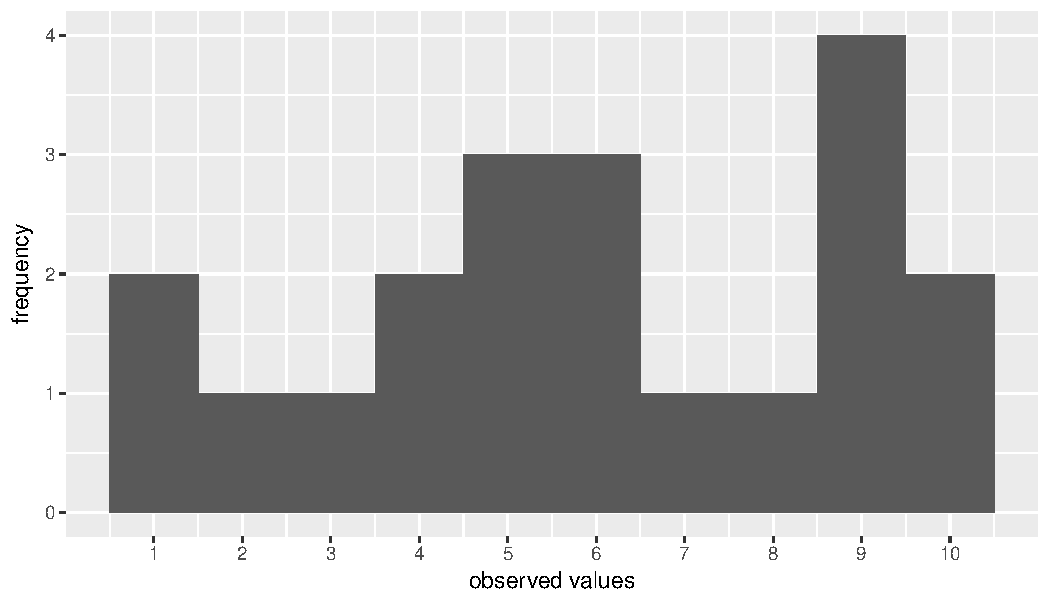
\includegraphics[width=\maxwidth]{figure/distr_1-1} 

}

\caption[A frequency plot]{A frequency plot}\label{fig:distr_1}
\end{figure}


\end{knitrout}

The data in the frequency table can also be represented using a frequency plot. Figure \ref{fig:distr_1} gives the same information, not in a table but in a graphical way. On the horizontal axis we see several possible values for age in years, and on the vertical axis we see the number of children (the count) that were observed for each particular age. Both the frequency table and the frequency plot tell us something about the \textit{distribution} of age in this imaginary town with 1000 children. For example, both tell us that the oldest child is 17 years old. Furthermore, we see that there are quite a lot of children with ages between 5 and 8, but not so many children with ages below 3 or above 14. The advantage of the table over the graph is that we can get the exact number of children of a particular age very easily. But on the other hand, the graph makes it easier to get a quick idea about the shape of the distribution, which is hard to make out from the table.

% <<distr_1, fig.height=4, echo=FALSE, fig.align='center', message=F, fig.cap='A frequency distribution' >>=
% set.seed(123)
% numbers <- runif(20, 1,10) %>%  round(0)
% data.frame(age) %>%
%         ggplot(aes(numbers)) + geom_bar()  
% +
%         xlab('observed values') + ylab('count')+
%         scale_x_continuous(breaks=seq(1,10))
% @

% Numeric variables have distributions. That means that if you put all the values you observed in order from low to high, you see a certain shape. For example, take the set of following numbers: numbers. If you plot these values on the horizontal axis, and how often they are observed (the \textit{frequency} or \textit{count}) on the vertical you get the frequency plot in Figure \ref{fig:distr_1}. Such a frequency plot is referred to as a \textit{bar chart}.

% Often a \textit{histogram} is plotted. A histogram is very much like a frequency plot or bar chart, except that groups of values can be taken together. Such a group of values is called a \textit{bin}. Figure \ref{fig:distr_2} shows the same data, but uses only 5 bins: for the first bin, we take values of 1 and 2, for the second bin we take values 3 and 4 together, etcetera, until we take vales 9 and 10 for the fifth bin. For each bin, we compute how often we observe the values in that bin. Histograms are also for continous data, for instance if we have values like 3.4, 2,1, etcetera. All values within a bin are defined by their rounded value. For instance, in Figure \ref{fig:distr_2}, all possible values between 2.5 and 4.5 will end up in the second bin. The \textit{binwidth} is here 2: all values between 2.5 and 4.5 are taken to lie in the second bin, and the distance between these values is $4.5-2.5=2$.

Instead of frequency plots, one often sees \textit{histograms}. Histograms contain the same information as frequency plots, except that \textit{groups of values} are taken together. Such a group of values is called a \textit{bin}. Figure \ref{fig:distr_2} shows the same age data, but uses only 9 bins: for the first bin, we take values of age 0 and 1 together, for the second bin we take ages 2 and 3 together, etcetera, until we take ages 16 and 17 together for the last bin. For each bin, we compute how often we observe the ages in that bin.

Histograms are very convenient for continuous data, for instance if we have values like 3.473, 2.154, etcetera. Or, more generally, for variables with values that have very low frequencies. Suppose that we had measured age not in years but in days. Then we could have had a data set of 1000 children where each and every child had a unique value for age. In that case, the length of the frequency table would be 1000 rows (each value observed only once) and the frequency plot would be very flat. By using age measured in years, what we have actually done is putting all children with an age less than 365 days into the first bin (age 0 years) and the children with an age of at least 365 but less than 730 days into the second bin (age 1 year). And so on. Thus, if you happen to have data with many many values with very low frequencies, consider binning the data, and using a histogram to visualise the distribution of your numeric variable.



\begin{knitrout}
\definecolor{shadecolor}{rgb}{0.969, 0.969, 0.969}\color{fgcolor}\begin{figure}

{\centering 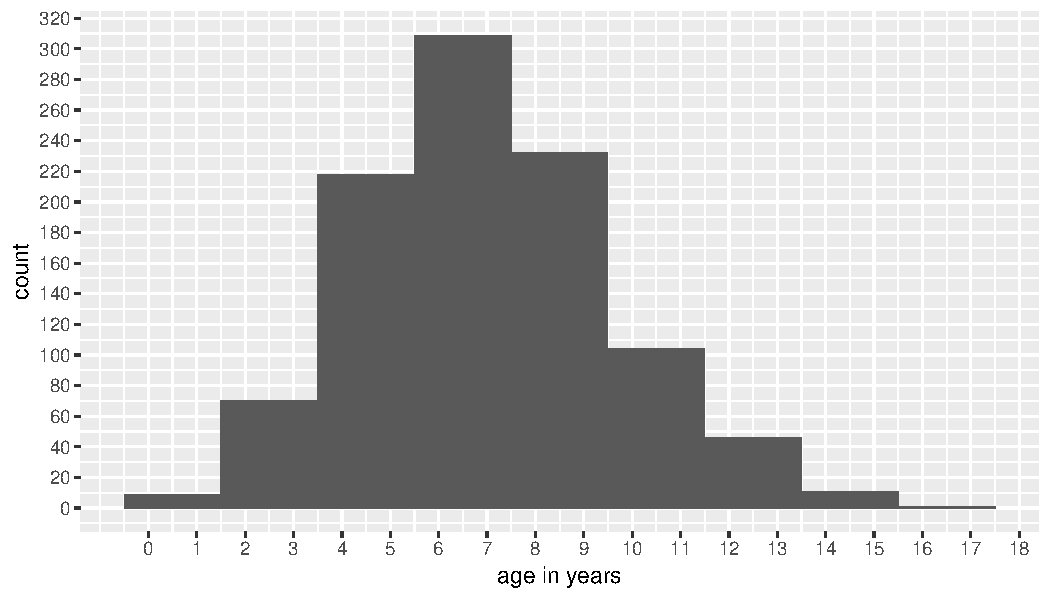
\includegraphics[width=\maxwidth]{figure/distr_2-1} 

}

\caption[A histogram]{A histogram}\label{fig:distr_2}
\end{figure}


\end{knitrout}



\section{Frequencies, proportions and cumulative frequencies and proportions}


When we have the frequency for each observed age, we can calculate the \textit{relative frequency} or \textit{proportion} of children that have that particular age. For example, when we look again at the frequencies in Table \ref{tab:frequency_1} we see that there are two children who have age 0. Given that there are in total 1000 children, we know that the \textit{proportion} of people with age 0 equals $\frac{2}{1000}=0.002$. Thus, the proportion is calculated by taking the frequency and dividing it by the total number.


We can also compute \textit{cumulative frequencies}. You get cumulative frequencies by accumulating (summing) frequencies. For instance, the cumulative frequency for the age of 3, is the frequency for age 3 plus all frequencies for younger ages. Thus, the cumulative frequency of age 3 equals 50 + 20 (for age 2) + 7 (for age 1) + 2 (for age 0) = 79. The cumulative frequencies for all ages are presented in Table \ref{tab:frequency_1}.

We can also compute \textit{cumulative proportions}: if we take for each age the proportion of people who have that age \textit{or less}, we get the fifth column in Table \ref{tab:frequency_1}. For example, for age 2, we see that there are 20 children with an age of 2. This corresponds to a proportion of 0.020 of all children. Furthermore, there are 9 children who have an even younger age. The proportion of children with an age of 1 equals 0.007, and the proportion of children with an age of 0 equals 0.002. Therefore, the proportion of all children with an age of 2 or less equals $0.020+0.007+0.002=0.029$, which is called the cumulative proportion for the age of 2.


\section{Frequencies and proportions in R}

The \texttt{mtcars} data set contains information about a number of cars: miles per gallon (\texttt{mpg}), number of cylinders (\texttt{cyl}), etcetera. 

\begin{knitrout}
\definecolor{shadecolor}{rgb}{0.969, 0.969, 0.969}\color{fgcolor}\begin{kframe}
\begin{alltt}
\hlstd{mtcars}
\end{alltt}
\begin{verbatim}
##                      mpg cyl  disp  hp drat    wt  qsec vs am gear carb
## Mazda RX4           21.0   6 160.0 110 3.90 2.620 16.46  0  1    4    4
## Mazda RX4 Wag       21.0   6 160.0 110 3.90 2.875 17.02  0  1    4    4
## Datsun 710          22.8   4 108.0  93 3.85 2.320 18.61  1  1    4    1
## Hornet 4 Drive      21.4   6 258.0 110 3.08 3.215 19.44  1  0    3    1
## Hornet Sportabout   18.7   8 360.0 175 3.15 3.440 17.02  0  0    3    2
## Valiant             18.1   6 225.0 105 2.76 3.460 20.22  1  0    3    1
## Duster 360          14.3   8 360.0 245 3.21 3.570 15.84  0  0    3    4
## Merc 240D           24.4   4 146.7  62 3.69 3.190 20.00  1  0    4    2
## Merc 230            22.8   4 140.8  95 3.92 3.150 22.90  1  0    4    2
## Merc 280            19.2   6 167.6 123 3.92 3.440 18.30  1  0    4    4
## Merc 280C           17.8   6 167.6 123 3.92 3.440 18.90  1  0    4    4
## Merc 450SE          16.4   8 275.8 180 3.07 4.070 17.40  0  0    3    3
## Merc 450SL          17.3   8 275.8 180 3.07 3.730 17.60  0  0    3    3
## Merc 450SLC         15.2   8 275.8 180 3.07 3.780 18.00  0  0    3    3
## Cadillac Fleetwood  10.4   8 472.0 205 2.93 5.250 17.98  0  0    3    4
## Lincoln Continental 10.4   8 460.0 215 3.00 5.424 17.82  0  0    3    4
## Chrysler Imperial   14.7   8 440.0 230 3.23 5.345 17.42  0  0    3    4
## Fiat 128            32.4   4  78.7  66 4.08 2.200 19.47  1  1    4    1
## Honda Civic         30.4   4  75.7  52 4.93 1.615 18.52  1  1    4    2
## Toyota Corolla      33.9   4  71.1  65 4.22 1.835 19.90  1  1    4    1
## Toyota Corona       21.5   4 120.1  97 3.70 2.465 20.01  1  0    3    1
## Dodge Challenger    15.5   8 318.0 150 2.76 3.520 16.87  0  0    3    2
## AMC Javelin         15.2   8 304.0 150 3.15 3.435 17.30  0  0    3    2
## Camaro Z28          13.3   8 350.0 245 3.73 3.840 15.41  0  0    3    4
## Pontiac Firebird    19.2   8 400.0 175 3.08 3.845 17.05  0  0    3    2
## Fiat X1-9           27.3   4  79.0  66 4.08 1.935 18.90  1  1    4    1
## Porsche 914-2       26.0   4 120.3  91 4.43 2.140 16.70  0  1    5    2
## Lotus Europa        30.4   4  95.1 113 3.77 1.513 16.90  1  1    5    2
## Ford Pantera L      15.8   8 351.0 264 4.22 3.170 14.50  0  1    5    4
## Ferrari Dino        19.7   6 145.0 175 3.62 2.770 15.50  0  1    5    6
## Maserati Bora       15.0   8 301.0 335 3.54 3.570 14.60  0  1    5    8
## Volvo 142E          21.4   4 121.0 109 4.11 2.780 18.60  1  1    4    2
\end{verbatim}
\end{kframe}
\end{knitrout}

The object is a data frame. We can turn it into a tibble as follows:

\begin{knitrout}
\definecolor{shadecolor}{rgb}{0.969, 0.969, 0.969}\color{fgcolor}\begin{kframe}
\begin{alltt}
\hlstd{mtcars} \hlkwb{<-} \hlstd{mtcars} \hlopt \hlkwd{as_tibble}\hlstd{()}
\end{alltt}
\end{kframe}
\end{knitrout}

The function \texttt{as\_tibble()} is available when you load the \texttt{tidyverse} package. From now on, we assume that you load the \texttt{tidyverse} package at the start of every R session.

If we want to know how many cars belong to which category of number of cylinders, we can use the function \texttt{count()}:

\begin{knitrout}
\definecolor{shadecolor}{rgb}{0.969, 0.969, 0.969}\color{fgcolor}\begin{kframe}
\begin{alltt}
\hlstd{mtcars} \hlopt
  \hlkwd{count}\hlstd{(cyl)}
\end{alltt}
\begin{verbatim}
## # A tibble: 3 x 2
##     cyl     n
##   <dbl> <int>
## 1     4    11
## 2     6     7
## 3     8    14
\end{verbatim}
\end{kframe}
\end{knitrout}

The new variable \texttt{n} is the frequency. We see that the value 4 occurs 11 times, the value 6 occurs 7 times and the value 8 occurs 14 times. Thus, in this data set there are 11 cars with 4 cylinders, 7 cars with 6 cylinders, and 14 cars with 8 cylinders. 

We obtain proportions when we divide the frequencies by the total number of cars (the sum of all the values in the \texttt{n} variable):

\begin{knitrout}
\definecolor{shadecolor}{rgb}{0.969, 0.969, 0.969}\color{fgcolor}\begin{kframe}
\begin{alltt}
\hlstd{mtcars} \hlopt
  \hlkwd{count}\hlstd{(cyl)} \hlopt
  \hlkwd{mutate}\hlstd{(}\hlkwc{proportion} \hlstd{= n}\hlopt{/}\hlkwd{sum}\hlstd{(n))}
\end{alltt}
\begin{verbatim}
## # A tibble: 3 x 3
##     cyl     n proportion
##   <dbl> <int>      <dbl>
## 1     4    11      0.344
## 2     6     7      0.219
## 3     8    14      0.438
\end{verbatim}
\end{kframe}
\end{knitrout}

Cumulative frequencies and cumulative proportions can be obtained using the \texttt{cumsum()} function:

\begin{knitrout}
\definecolor{shadecolor}{rgb}{0.969, 0.969, 0.969}\color{fgcolor}\begin{kframe}
\begin{alltt}
\hlstd{mtcars} \hlopt
  \hlkwd{count}\hlstd{(cyl)} \hlopt
  \hlkwd{mutate}\hlstd{(}\hlkwc{proportion} \hlstd{= n}\hlopt{/}\hlkwd{sum}\hlstd{(n))} \hlopt
  \hlkwd{mutate}\hlstd{(}\hlkwc{cumfreq} \hlstd{=} \hlkwd{cumsum}\hlstd{(n),}
         \hlkwc{cumprop} \hlstd{=} \hlkwd{cumsum}\hlstd{(proportion))}
\end{alltt}
\begin{verbatim}
## # A tibble: 3 x 5
##     cyl     n proportion cumfreq cumprop
##   <dbl> <int>      <dbl>   <int>   <dbl>
## 1     4    11      0.344      11   0.344
## 2     6     7      0.219      18   0.562
## 3     8    14      0.438      32   1
\end{verbatim}
\end{kframe}
\end{knitrout}


A frequency plot can be made using ggplot combined with \texttt{geom\_line()}:

\begin{knitrout}
\definecolor{shadecolor}{rgb}{0.969, 0.969, 0.969}\color{fgcolor}\begin{kframe}
\begin{alltt}
\hlstd{mtcars} \hlopt
  \hlkwd{count}\hlstd{(cyl)} \hlopt
  \hlkwd{mutate}\hlstd{(}\hlkwc{proportion} \hlstd{= n}\hlopt{/}\hlkwd{sum}\hlstd{(n))} \hlopt
  \hlkwd{ggplot}\hlstd{(}\hlkwd{aes}\hlstd{(}\hlkwc{x} \hlstd{= cyl,} \hlkwc{y} \hlstd{= n))} \hlopt{+}
  \hlkwd{geom_line}\hlstd{()}
\end{alltt}
\end{kframe}
\end{knitrout}

A histogram of the \texttt{mpg} variable can be made using \texttt{geom\_histogram()}:

\begin{knitrout}
\definecolor{shadecolor}{rgb}{0.969, 0.969, 0.969}\color{fgcolor}\begin{kframe}
\begin{alltt}
\hlstd{mtcars} \hlopt
  \hlkwd{ggplot}\hlstd{(}\hlkwd{aes}\hlstd{(}\hlkwc{x} \hlstd{= mpg))} \hlopt{+}
  \hlkwd{geom_histogram}\hlstd{(}\hlkwc{breaks} \hlstd{=} \hlkwd{seq}\hlstd{(}\hlnum{5}\hlstd{,} \hlnum{40}\hlstd{,} \hlnum{5}\hlstd{))}
\end{alltt}
\end{kframe}
\end{knitrout}

It is wise to play around with the number of bins that you'd like to make, or with the boundaries of the bins. Here we choose boundaries $5, 10, 15, \dots, 40$.

\section{Quartiles, quantiles and percentiles}

Suppose we want to split the group of 1000 children into 4 equally-sized subgroups, with the 25\% youngest children in the first group, the 25\% oldest children in the last group, and the remaining 50\% of the children in two equally sized middle groups. What ages should we then use to divide the groups? First, we can order the 1000 children on the basis of their age: the youngest first, and the oldest last. We could then use the concept of \textit{quartiles} (from quarter, a fourth) to divide the group in four. In order to break up all ages into 4 subgroups, we need 3 points to make the division, and these three points are called quartiles. The first quartile is the value below which 25\% of the observations fall, the second quartile is the value below which 50\% of the observations fall, and the third quartile is the value below which 75\% of the observations fall.\footnote{The fourth quartile would be the value below which \textit{all} values are, so that would be the largest value in the row (the age of the last child in the row).}

Let's first look at a smaller but similar problem. For example, suppose your observed values are {10, 5, 6, 21, 11, 1, 7, 9}. You first order them from low to high so that you obtain {1, 5, 6, 7, 9, 10, 11, 21}. You have 8 values, so the first 25\% of your values are the first two. The highest value of these two equals 5, and this we define as our first quartile.\footnote{Note that we could also choose to use 6, because 1 and 5 are lower than 6. Don't worry, the method that we show here to compute quartiles is only one way of doing it. In your life, you might stumble upon alternative ways to determine quartiles. These are just arbitrary agreements made by human beings. They can result in different outcomes when you have small data sets, but usually not when you have large data sets.} We find the second quartile by looking at the values of the first 50\% of the observations, so 4 values. The first 4 values are 1, 5, 6, and 7. The last of these is 7, so that is our second quartile. The first 75\% of the observations are 1, 5 ,6 ,7 , 9, and 10. The value last in line is 10, so our fourth quartile is 10.

The quartiles as defined here can also be found graphically, using cumulative proportions. Figure \ref{fig:quartile_1} shows for each observed value the cumulative proportion. It also shows where the cumulative proportions are equal to 0.25, 0.50 and 0.75. We see that the 0.25 line intersects the other line at the value of 5. This is the first quartile. The 0.50 line intersects the other line at a value of 7, and the 0.75 line intersects at a value of 10. The three percentiles are therefore 5, 7 and 10.


\begin{figure}

{\centering 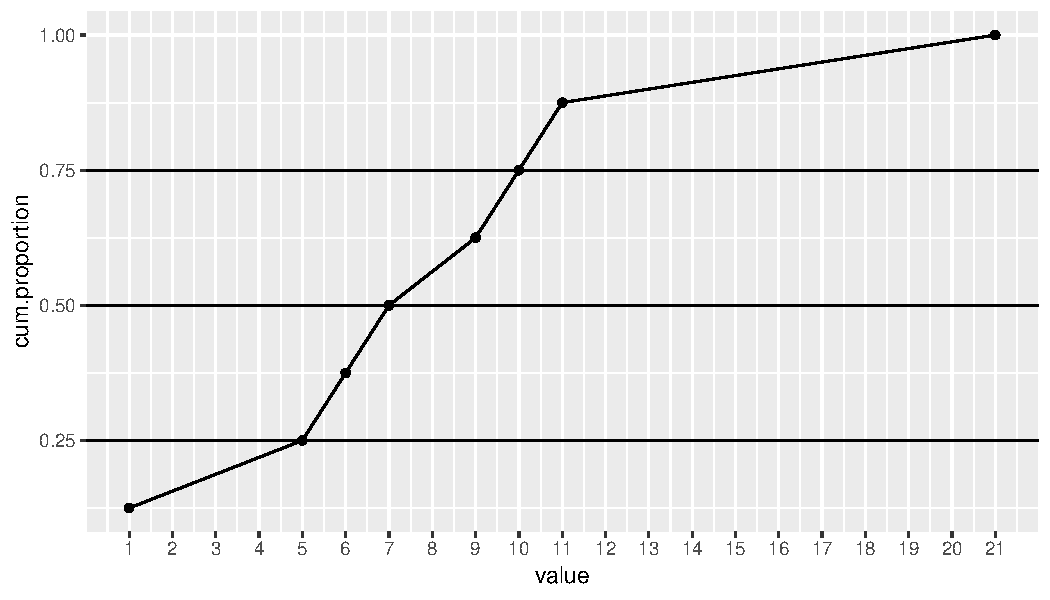
\includegraphics[width=\maxwidth]{figure/quartile_1-1} 

}

\caption[Cumulative proportions]{Cumulative proportions.}\label{fig:quartile_1}
\end{figure}



If you have a large data set, the graphical way is far easier than doing it by hand. If we plot the cumulative proportions for the ages of the 1000 children, we obtain Figure \ref{fig:quartile_2}. We see a nice S-shaped curve. We also see that the three horizontal quartile lines no longer intersect the curve at specific values, so what do we do? By eye-balling we can find that the first quartile is somewhere between 4 and 5. But which value should we give to the quartile? If we look at the cumulative proportion for an age of 4, we see that its value is slightly below the 0.25 point. Thus, the proportion of children with age 4 or younger is lower than 0.25. This means that the child that happens to be the 250th cannot be 4 years old. If we look at the cumulative proportion of age 5, we see that its value is slightly above 0.25. This means that the proportion of children that is 5 years old or younger is slightly more than 0.25. Therefore, of the the total of 1000 children, the 250th child must have age 5. Thus, by definition, the first quantile is 5. 
The second quartile is somewhere between 6 an 7, so by using the same reasoning as for the first quartile we know that 50\% of the youngest children is 7 years old or younger. The third quartile is somewhere between 8 and 9 and this tells us that the youngest 75\% of the children is age 9 or younger. Thus, we can call 5, 7 and 9 our three quartiles.



\begin{figure}

{\centering 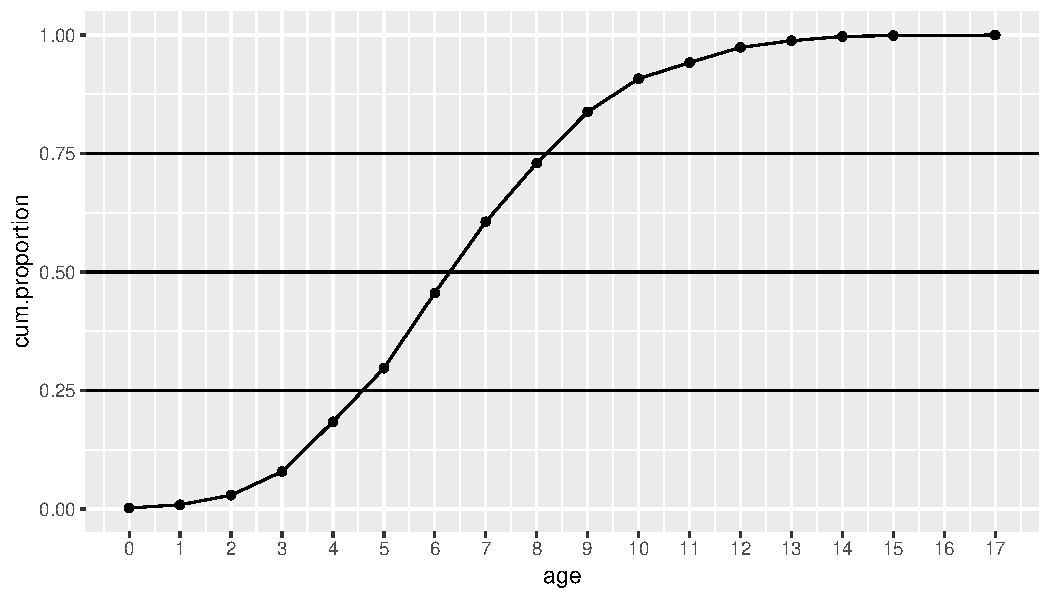
\includegraphics[width=\maxwidth]{figure/quartile_2-1} 

}

\caption[Cumulative proportions]{Cumulative proportions.}\label{fig:quartile_2}
\end{figure}




Alternatively, we could also use the frequency table (Table \ref{tab:frequency_1}). First, if we want to have 25\% of the children that are the youngest, and we know that we have 1000 children in total, we should have $0.25 \times 1000=250$ children in the first group. So if were to put all the children in a row, ordered from youngest to oldest, we want to know the age of the 250th child.

In order to find the age of this 250th child, and we look at Table \ref{tab:frequency_1}, we see that 29.7\% of the children have an age of 5 or less (297 children), and 18.4\% of the children have an age of 4 or less (184 children). This tells us that, since 250 comes after 184, the 250th child must be older than 4, and because 250 comes before 297, it must be younger than or equal to 5, hence the child is 5 years old.

Furthermore, if we want to find a cut-off age for the oldest 25\%, we see from the table, that 83.8\% of the children (838 children) have an age of 9 or less, and 73.0\% of the children (730) have an age of 8 or less. Therefore, the age of the 750th child (when ordered from youngest to oldest) must be 9.


What we just did for quartiles, (i.e. 0.25, 0.50, 0.75) we can do for any proportion between 0 and 1. We then no longer call them quartiles, but \textit{quantiles}. A quantile is the value below which a given proportion of observations in a group of observations fall. From this table it is easy to see that a proportion of 0.606 of the children have an age of 7 or less. Thus, the 0.606 quantile is 7. One often also sees \textit{percentiles}. Percentiles are very much like quantiles, except that they refer to percentages rather than proportions. Thus, the 20th percentile is the same as the 0.20 quantile. And the 0.81 quantile is the same as the 81st percentile.

The reason that quartiles, quantiles and percentiles are important is that they are very short ways of saying something about a distribution. Remember that the best way to represent a distribution is either a frequency table or a frequency plot. However, since they can take up quite a lot of space sometimes, one needs other ways to briefly summarise a distribution. Saying that "the third quartile is 454" is a condensed way of saying that "75\% of the values is either 454 or lower". In the next sections, we look at other ways of summarising information about distributions.

Another way in which quantiles and percentiles are used is to say something about \textit{individuals}, relative to a group. Suppose a student has done a test and she comes home saying she scored in the 76th percentile of her class. What does that mean? Well, you don't know her score exactly, but you do know that of her classmates, 76 percent had the same score or lower. That means she did pretty well, compared to the others, since only 24 percent had a higher score.

% \subsection{Exercises}
% 
% <<frequency_2, fig.height=4, echo=FALSE, fig.align='center', fig.cap='A frequency distribution', results='asis' >>=
% set.seed(123)
% x <- rpois(200, 3)
% data.frame(x) %>% 
%   group_by(x) %>%
%   summarise(frequency = n(),
%             proportion = n()/200) %>%
%   mutate(cum.proportion = cumsum(proportion)) %>%
%   xtable(caption = "Freqency table for x, with proportions and cumulative proportions.", 
%          label = "tab:frequency_2", 
%          digits = 3) %>%
%   print(include.rownames = F, caption.placement = "top")
% @
% 
% \begin{enumerate}
% \item Look at Table \ref{tab:frequency_2}. Determine the 10th quantile for variable \textbf{x}.
% 
% \item Determine the 95th percentile.
% 
% \item Determine the first quartile.
% 
% \item Determine the second quartile.
% 
% \item Determine the 50th percentile.
% 
% \item Determine the third quantile.
% 
% \item Determine the 0.75 quantile.
% 
% \item Suppose we have the values {6,5,4,8,6,5,6,4,5,6,7,8}. Determine the third quartile.
% 
% \item Suppose we have the values {4,4,4,8,6,4,6,4,5,6,7,8}. Determine the third quartile.
% 
% \item From Figure \ref{fig:quartile_3}, determine the 30th, 40th and 90th percentiles.
% 
% <<quartile_3, fig.height=4, echo=FALSE, fig.align='center', fig.cap='Cumulative proportions.', results='asis' >>=
% 
% value = rchisq(100, 4) %>% round()
% tibble(value) %>% 
%   group_by(value) %>%
%   summarise (frequency = n(),
%              proportion= n()/100) %>%
%   mutate(cum.proportion = cumsum(proportion)) %>%
%   ggplot(aes(value, cum.proportion)) +
%   geom_line() + 
%   geom_point() +
%   scale_y_continuous(breaks = seq(0, 1, 0.1)) +
%   scale_x_continuous(breaks = 0:17) +
%   geom_hline(yintercept = c(0.30, 0.40, 0.90))
% @
% 
% \item Suppose yesterday you did an IQ test, together with 999 other students. Today you hear that you scored 100 points. They tell you that the 8th percentile was a score of 80, and the 9th percentile was a score of 100. What does that tell you about your performance yesterday?
% 
% 
% \end{enumerate}
% 
% 
% \subsection{Answers}
% 
% \begin{enumerate}
% 
% \item
% 1
% \item
% 6
% \item
% 2
% \item
% 3
% \item
% 3
% \item
% 4
% \item
% 4
% \item
% ordered series: 445 556 666 788, last value of third quart: 6
% \item
% orderd series: 444 445 666 788, last value of third quart: 6
% 
% \item
% 2, 2 and 7
% 
% \item
% 
% Nine percent of my fellow students scored the same or lower than I did on the exam, so 91 percent did better. I did not do so well.
% 
% \end{enumerate}
% 

\section{Quantiles in R}

Obtaining quartiles, quantiles and percentiles can be done with the \texttt{quantile()} function:

\begin{knitrout}
\definecolor{shadecolor}{rgb}{0.969, 0.969, 0.969}\color{fgcolor}\begin{kframe}
\begin{alltt}
\hlkwd{quantile}\hlstd{(mtcars}\hlopt{$}\hlstd{mpg,}
         \hlkwc{probs} \hlstd{=} \hlkwd{c}\hlstd{(}\hlnum{0.25}\hlstd{,} \hlnum{0.50}\hlstd{,} \hlnum{0.75}\hlstd{,} \hlnum{0.90}\hlstd{))}
\end{alltt}
\begin{verbatim}
##    25%    50%    75%    90% 
## 15.425 19.200 22.800 30.090
\end{verbatim}
\end{kframe}
\end{knitrout}






\section{Measures of central tendency}

The mean, the median and the mode are three different measures that say something about the \textit{central tendency} of a distribution. If you have a series of values: around which value do they tend to cluster?

\subsection{The mean}
Suppose we have the values 1, 2 and 3, then we compute the mean by first adding these numbers and then divide them by the number of values we have. In this case we have three values, so the mean is equal to $(1 + 2 + 3)/3 = 2$. In statistical formulas, the mean of a variable is indicated by a bar above that variable. So if our values of variable $Y$ are 1, 2 and 3, then we denote the mean by $\widebar{Y}$ (pronounced as 'y-bar'). When taking the sum of a set of values, statistical formulas show the summation sign $\Sigma$ (the Greek letter sigma). So we often see the following formula for the mean of a set of $n$ values for variable $Y$\footnote{Variables are symbolised by capitals, e.g., $Y$. Specific values of a variable are indicated in lowercase, e.g., $y$.}:

\begin{equation}
\widebar{Y} = \frac{\Sigma_{i=1}^n Y_i}{n}
\end{equation}

In words, in order to compute $\widebar{Y}$, we take every value for variable $Y$ from $i=1$ to $i=n$ and sum them, and the result is divided by $n$. Suppose we have variable $Y$ with the values {6, -3, and 21}, then the mean of $Y$ equals:

\begin{equation}
\widebar{Y} = \frac {  \Sigma_{i} Y_i} {n} =    \frac{Y_1 + Y_2 + Y_3}{n} = \frac{6 + (-3) + 21}{3} = \frac{24}{3} = 8
\end{equation}







\subsection{The median}
The mean is only one of the measures of central tendency. An alternative measure of central tendency is the \textit{median}. The median is nothing but the middle value of an ordered series. Suppose we have the values 45, 567, and 23. Then what value lies in the middle when ordered? Let's first order them from small to large to get a better look. We then get 23, 45 and 567. Then it's easy to see that the value in the middle is 45.

Suppose we have the values 45, 45, 45, 65, and 23. What is the middle value when ordered? We first order them again and see what value is in the middle: 23, 45, 45, 45 and 65. Obviously now 45 is the median. You can also see that half of the values is equal or smaller than this value, and half of the values is equal or larger than this value. The median therefore is the same as the second quartile.

What if we have two values in the middle? Suppose we have the values 46, 56, 45 and 34. If we order them we get 34, 45, 46 and 56. Now there are two values in the middle: 45 and 46. In that case, we take the mean of these two middle values, so the median is 45.5. 

When do you use a median and when do you use a mean? For numeric variables that have a more or less symmetric distribution (i.e., a frequency plot that is more or less symmetric), the mean is most often used. Actually, for distributions that are more or less symmetric the mean and median are very similar. For numeric variables that do not have a symmetric distribution, it is usually more informative to use the median. An example of such a situation is income. Figure \ref{fig:median} shows a typical distribution of yearly income. The distribution is highly asymmetric, it is severely skewed to the right. The bulk of the values are between 20,000 and 40,000, with only a very few extreme values on the high end. Even though there are only a few people with a very high income, the few high values have a huge effect on the mean.

\begin{figure}

{\centering 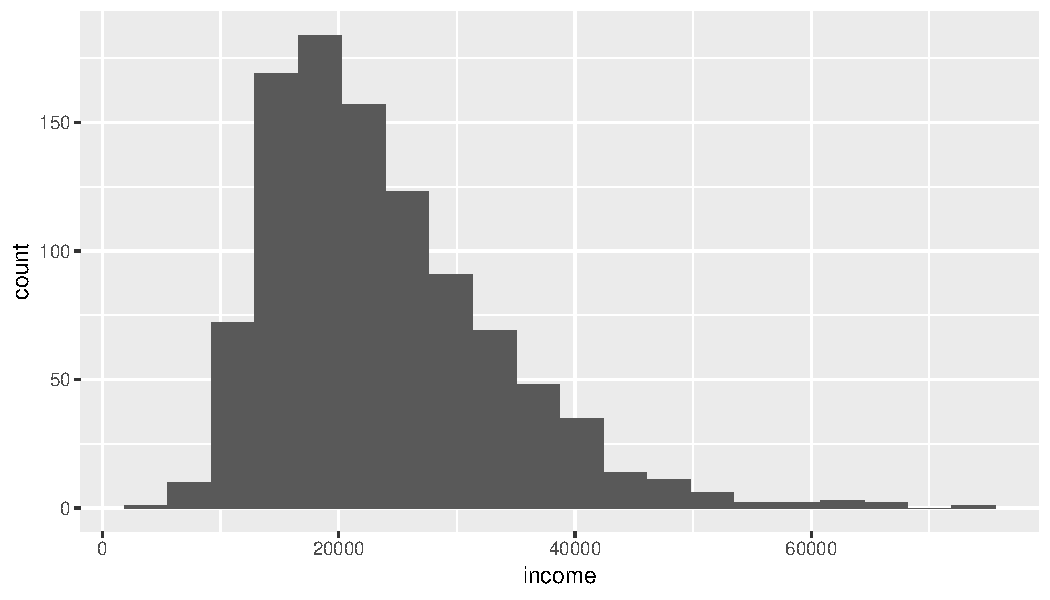
\includegraphics[width=\maxwidth]{figure/median-1} 

}

\caption[Distribution of yearly income]{Distribution of yearly income.}\label{fig:median}
\end{figure}



The mean of the distribution turns out to be 23604. The largest value in the distribution is an income of 75051. Imagine what would happen to the mean and the median if we would change only this one value, that is, the highest observed income. Which would be most affected, do you think: the mean or the median?



Well, if we would change this value into 85051, you see an immediate impact on the mean: the mean is then 23614. This means that the mean is very sensitive to extreme values. One single change in a data set can have a huge effect on the mean. The median on the other hand is much more stable. The median remains unaffected by changes in the extremes. This because it only looks at the middle value. The middle value is unaffected by a change in the extreme values, as long as the order of the values remains the same and the middle value remains the same.

This can be seen even more clearly by looking at the example in Table \ref{tab:median_2}. There we have three values, X1, X2 and X3, for which we compute both the mean and the median. First, suppose we have the values 4, 5, and 8 (like in the first row of Table \ref{tab:median_2}). Obviously, the median is 5. Next, instead of 4, 5 and 8, we could have values 4, 5 and 80, or 4, 5 and 800, or 4, 5 and 8000. Regardless, the middle value of this series remains 5. In contrast, the mean would be very much affected by having either an 8, an 80, an 800 or an 8000 in the series. In sum: the median is a more stable measure of central tendency than the mean.


% latex table generated in R 4.0.3 by xtable 1.8-4 package
% Sun Jan 31 16:36:25 2021
\begin{table}[ht]
\centering
\caption{Four series of values and their respective medians and means.} 
\label{tab:median_2}
\begin{tabular}{rrrrr}
  \hline
X1 & X2 & X3 & median & mean \\ 
  \hline
4 & 5 & 8 & 5 & 5.7 \\ 
  4 & 5 & 80 & 5 & 29.7 \\ 
  4 & 5 & 800 & 5 & 269.7 \\ 
  4 & 5 & 8000 & 5 & 2669.7 \\ 
   \hline
\end{tabular}
\end{table}




\subsection{The mode}
A third measure of central tendency is the \textit{mode}. The mode is defined as the value that we see most frequently in a series of values. For example, if we have the series 4, 7, 5, 5, 6, 6, 6, 4, then the value observed most often is 6 (three times). Modes are easily inferred from frequency tables: the value with the largest frequency is the mode. They are also easily inferred from frequency plots: the value on the horizontal axis for which we see the highest count (on the vertical axis).

The mode can also be determined for categorical variables. If we have the observed values 'Dutch', 'Danish', 'Dutch', and 'Chinese', the mode is 'Dutch' because that is the value that is observed most often.

If we look back at the distribution in Figure \ref{fig:median}, we see that the peak of the distribution is around the value of 19,000. However, whether this is the mode, we cannot say. Because income is a more or less continuous variable, every value observed in the Figure occurs only once: there is no value of income with a frequency more than 1. So technically, there is no mode. However, if we split the values into 20 bins, like we did for the histogram in Figure \ref{fig:median}, we see that the fifth bin has the highest frequency. In this bin there are values between 17000 and 21000, so our mode could be around there. If we really want a specific value, we could decide to take the average value in the fifth bin. There are many other statistical tricks to find a value for the mode, where technically there is none. The point is that for the mode, we're looking for the value or the range of values that are most frequent. Graphically, it is the value under the peak of the distribution. Similar to the median, the mode is also quite stable: it is not affected by extreme values and is therefore to be preferred over the mean in the case of asymmetric distributions.



% \subsection{Exercises}
% 
% \begin{enumerate}
% 
% \item If we have values 56, 78, 23 and 45, what is the mean?
% 
% \item If we have values 56, 78, 23 and 45, what is the median?
% 
% \item If we have values 56, 23, 78, 23 and 45, what is the mode?
% 
% \item Figure \ref{fig:mode} shows a distribution of systolic bloodpressure measures in older men. What would be more or less the mode of these values?
% 
% <<mode, fig.height=4, echo=FALSE, fig.align='center', fig.cap='Distribution of systolic bloodpressure.', results='asis' >>=
% set.seed(34)
% sbp <- rnorm(100, 5, 0.2) %>% exp()
% tibble(sbp) %>%
%   ggplot(aes(sbp)) +
%   geom_histogram(bins = 10) + 
%   xlab("Systolic bloodpressure")
% @
% 
% \item Figure \ref{fig:quartile_3} shows a distribution of values. What would be more or less the median of these values?
% 
% \item Figure \ref{fig:mode2} shows a distribution of number of bicycles for 100 households. If you could choose only one measure to describe this distribution, what would you choose to report: the mean, the mode or the median? Motivate your answer.
% 
% <<mode2, fig.height=4, echo=FALSE, fig.align='center', fig.cap='Distribution of number of bicycles per household.', results='asis' >>=
% set.seed(34)
% bicycles <- rpois(100, 1) %>% round()
% tibble(bicycles) %>%
%   ggplot(aes(bicycles)) +
%   geom_histogram(bins = 10, binwidth = 1) +
%   scale_x_continuous(breaks = seq(0, 10))
% @
% 
% 
% 
% \end{enumerate}
% 
% 
% \subsection{Answers}
% 
% \begin{enumerate}
% \item mean(c(56, 78, 23,45))
% \item median(c(56, 78, 23,45))
% \item  23
% \item 140
% \item 3
% \item The median. Because the distribution is very skew and in that case the mean would be relatively high, because it is influenced by a few households with very many bicycles. The mode would not say very much other than that 0 bicycles is the most common observation. But saying that half the households have 1 bicycle or lesswould be more informative than that. 
% 
% \end{enumerate}






\section{Relationship between measures of tendency and measurement level}

There is a close relationship between measures of tendency and measurement level. For numeric variables, all three measures of tendency are meaningful. Suppose you have the numeric variable age measured in years, with the values 56, 68, 68, 99 and 100. Then it is meaningful to say that the average age is 78.2 years, that the median age is 68 years, and that the mode is 68 years.

For ordinal variables, it is quite different. Suppose you have 5 T-shirts, with the following sizes: M, S, M, L, XL. Then what is the average size? There are no numeric values here to put in the algebraic formula. But we can determine the median: if we order the values from small to large we get the set S, M, M, L, XL and we see that the middle value is M. So M is our median in this case. \footnote{However, suppose that our collection of T-shirts had the following sizes: S, M, L, L. Then there would be no single middle value in we would have to average the M and L values, which would be impossible!} The other meaningful measure of tendency for ordinal variables is the mode.

For categorical variables, both the mean and the median are pointless to report. Suppose we have the nominal variable Study Programme with observed values "Medicine", "Engineering", "Engineering", "Mathematics", and "Biology". It would be impossible to derive a numerical mean, nor would it be possible to determine the middle value to determine the median, as there is no logical or natural order.\footnote{Unless you see one? But then it would not be a categorical value but an ordinal variable.} It is meaningful though to report a mode. It would be meaningful to state that the study programme mentioned most often in the news is "Psychology", or that the most popular study programme in India is "Engineering". Thus, for categorical variables, both dichotomous and nominal variables, only the mode is a meaningful measure of central tendency.

As stated earlier, the appearance of a variable in a data matrix can be quite misleading. Categorical variables and ordinal variables can often look like numeric variables, which makes it very tempting to compute means and medians where they are completely meaningless. Take a look at Table \ref{tab:modemedian}. It is entirely possible to compute the average University, Size, or Programme, but it would be utterly senseless to report these values.

It is entirely possible to compute the median University, Size, or Programme, but it is only meaningful to report the median for the variable Size, as Size is an ordinal variable. Reporting that the median size is equal to 2 is saying that about half of the study programmes is of medium size or small, and about half of the study programmes is of medium size or large.

It is entirely possible to compute the mode for the variables University, Size, or Programme, and it is always meaningful to report them. It is meaningful to say that in your data there is no University that is observed more than others. It is meaningful to report that most study programmes are of medium size, and that most study programmes are study programme number 2 (don't forget to look up and write down which study programme that actually is!).



% latex table generated in R 4.0.3 by xtable 1.8-4 package
% Sun Jan 31 16:36:25 2021
\begin{table}[ht]
\centering
\caption{Study programmes and their relative sizes (1=small, 2=medium, 3=large) for six different universities.} 
\label{tab:modemedian}
\begin{tabular}{rrr}
  \hline
University & Size & Programme \\ 
  \hline
1 & 1 & 2 \\ 
  2 & 3 & 2 \\ 
  3 & 2 & 3 \\ 
  4 & 2 & 3 \\ 
  5 & 3 & 4 \\ 
  6 & 2 & 1 \\ 
   \hline
\end{tabular}
\end{table}


\section{Measures of central tendency in R}

The mean and median for numeric variables can be obtained as follows:

\begin{knitrout}
\definecolor{shadecolor}{rgb}{0.969, 0.969, 0.969}\color{fgcolor}\begin{kframe}
\begin{alltt}
\hlstd{mtcars} \hlopt
  \hlkwd{summarise}\hlstd{(}\hlkwc{mean_cyl} \hlstd{=} \hlkwd{mean}\hlstd{(cyl),}
            \hlkwc{median_cyl} \hlstd{=} \hlkwd{median}\hlstd{(cyl))}
\end{alltt}
\begin{verbatim}
## # A tibble: 1 x 2
##   mean_cyl median_cyl
##      <dbl>      <dbl>
## 1     6.19          6
\end{verbatim}
\end{kframe}
\end{knitrout}


R does not have an in-built function to calculate modes. So we create our own function \texttt{getmode()}. This function takes a vector as input and gives the mode value as output.

\begin{knitrout}
\definecolor{shadecolor}{rgb}{0.969, 0.969, 0.969}\color{fgcolor}\begin{kframe}
\begin{alltt}
\hlstd{getmode} \hlkwb{<-} \hlkwa{function}\hlstd{(}\hlkwc{variable}\hlstd{)\{}
  \hlstd{unique_values} \hlkwb{<-} \hlkwd{unique}\hlstd{(variable)}
  \hlstd{unique_values[}
    \hlkwd{match}\hlstd{(variable, unique_values)} \hlopt
      \hlkwd{tabulate}\hlstd{()} \hlopt
      \hlkwd{which.max}\hlstd{()}
    \hlstd{]}
\hlstd{\}}

\hlstd{mtcars} \hlopt
  \hlkwd{summarise}\hlstd{(}\hlkwc{mode_cyl} \hlstd{=} \hlkwd{getmode}\hlstd{(cyl))}
\end{alltt}
\begin{verbatim}
## # A tibble: 1 x 1
##   mode_cyl
##      <dbl>
## 1        8
\end{verbatim}
\end{kframe}
\end{knitrout}




\section{Measures of variation}

Above we saw that we can summarise distributions by measures of central tendency. Here we discuss how we can summarise distributions of numeric variables by a measure that describes their \textit{variation}. Variables show variation, by definition, but how much variation do they actually show?

Suppose we measure the height of 3 children, and their heights (in cms) are 120, 120 and 120. There is no variation in height: all heights are the same. There are no differences. Then the average height is 120, the median height is 120, and the mode is 120. The variation is 0: non-existing, absent.

Now suppose their heights are 120, 120, 135. Now there are differences: one child is taller than the other two, who have the same height. There is some variation now. We know how to quantify the mean, which is 125, we know how to quantify the median, which is 120, and we know how to quantify the mode, which is also 120. But how do we quantify the variation? Is there a lot of variation, or just a little, and how do we measure it?

\subsection{Range and interquartile range}

One thing you could think of is measuring the distance or difference between the lowest value and the highest value. We call this the \textit{range}. The lowest value is 120, and the highest value is 135, so the range of the data is equal to $135-120=15$. As another example, suppose we have the values 20, 20, 21, 20, 19, 20 and 454. Then the range is equal to $454-19=435$. That's a large range, for a series of values that for the most part hardly differ from each other.

Instead of measuring the distance from the lowest to the highest value, we could also measure the distance between the first and the third quartile: how much does the third quartile \textit{deviate} from the first quartile? This distance or deviation is called the \textit{interquartile range} (IQR) or the \textit{interquartile distance}. Suppose that we have a large number of systolic blood pressure measurements, where 25\% are 120 or lower, and 75\% are 147 or lower, then the interquartile range is equal to $147-120=27$.

Thus, we can measure variation using the range or the interquartile range. A third measure for variation is \textit{variance}, and variance is based on the \textit{sum of squares}.

\subsection{Sum of squares}

What we call a sum of squares is actually a sum of squared deviations. But deviations from what? We could for instance be interested in how much the values 120, 120, 135 vary around the mean of these values. The mean of these three values equals 125. The first value differs $120-125= -5$, the second value also differs $120-125= -5$, and the third value differs $135-125= 10$.

Whenever we look at deviations from the mean, some deviations are positive and some deviations will be negative (except when there is no variation). If we want to measure variation, it should not matter whether deviations are positive or negative: any deviation should add to the total variation in a positive way. Moreover, if we would add up all deviations from the mean, we would always end up with 0, as you can see in our example. Adding up -5, -5 and +10 would lead to a sum of 0. This would mean no variation. However, as you can see, there is variation. So that is why we would better make all deviations positive, and this can be done by taking the square of the deviations, since a negative number squared is always positive. So for our three values 120, 120 and 135, we get the deviations -5, -5 and +10, and if we square these deviations, we get 25, 25 and 100. If we add these three squares, we obtain the sum 150. This is a sum of squared differences, or sum of squares.

In most cases, the sum of squares (SS) refers to the sum of squared deviations from the mean. In brief, suppose you have $n$ values of a variable $Y$, you first take the mean of those values (this is $\widebar{Y}$), you subtract this mean from each of these $n$ values ($Y_i-\widebar{Y}$), then you take the squares of these deviations, $(Y_i-\widebar{Y})^2$, and then add them up (take the sum of these squared deviations, $\Sigma (Y_i-\widebar{Y})^2$. In formula form, this process looks like:

\begin{equation}
SS = \Sigma_i^n (Y_i-\widebar{Y})^2
\end{equation}

As an example, suppose you have the values 10, 11 and 12, then the mean is 11. Then the deviations from the mean are -1, 0 and +1. If you square them you get $(-1)^2=1$, $0^2=0$ and $(+1)^2=1$, and if you sum these three values, you get $SS=1+0+1=2$. In formula form:


\begin{eqnarray}
SS &=& (Y_1-\widebar{Y})^2 + (Y_2-\widebar{Y})^2 +(Y_3-\widebar{Y})^2 \\
&=& (10-11)^2 + (11-11)^2 +(12-11)^2 = (-1)^2 + 0^2 + 1^2=2 \nonumber
\end{eqnarray}

Now let's use some values that are more different from each other, but with the same mean. Suppose you have the values 9, 11 and 13. The average value is still 11, but the deviations from the mean are larger. The deviations from 11 are -2, 0 and +2. Taking the squares, you get $(-2)^2=4$, $0^2=0$ and $(+2)^2=4$ and if you add them you get $SS=4+0+4=8$.

\begin{eqnarray}
SS &=& (Y_1-\widebar{Y})^2 + (Y_2-\widebar{Y})^2 +(Y_3-\widebar{Y})^2 \\
&=& (9-11)^2 + (11-11)^2 +(13-11)^2= (-2)^2 + 0^2 + 2^2=8 \nonumber
\end{eqnarray}

Thus, the more the values differ from each other, the larger the deviations from the mean. And the larger the deviations from the mean, the larger the sum of squares. The sum of squares is therefore a nice measure of how much values differ from each other.

\subsection{Variance and standard deviation} \label{sec:standarddeviation}

The sum of squares can be seen as a measure of total variation: all (squared) deviations from a certain value are added up. This means that the more data values you have, the larger the sum of squares. Often-times, you are not interested in the total variation, but you're interested in the average variation. Suppose we have the values 10, 11 and 24. The mean is then $45/3=15$. We have two values that are smaller than the mean and one value that is larger than the mean, so two negative deviations and one positive deviation. Squaring them makes them all positive. The squared deviations are 25, 16, and 81. The third value has a huge squared deviation (81) compared to the other two values. If we take the \textit{average} squared deviation, we get $(25+16+81)/3 \approx 40.67$. So the average squared deviation is equal to 40.67. This value is called the \textit{variance}. So the variance of a bunch of values is nothing but the $SS$ divided by the number of values, $n$. The variance is \textit{the average squared deviation from the mean}. The symbol used for the variance is usually $\sigma^2$ (pronounced as 'sigma squared').\footnote{Online you will often find the formula $\frac{\Sigma_i (Y_i-\widebar{Y})^2}{n-1}$. The difference is that here we are talking about the definition of the variance of an observed variable $Y$, and that elsewhere one talks about trying to figure out what the variance might be of all values of $Y$ when we only see a small portion of the values of $Y$. When we use all values of $Y$, we talk about the \textit{population} variance, denoted by $\sigma^2$. When we only see a small part of the values of $Y$, we talk about a \textit{sample} of $Y$-values. We will come back to the distinction between population variance and sample variance and why they differ in Chapter \ref{chap:mean}.}

\begin{equation}
\mathrm{Var}(Y) = \frac{SS}{n}= \frac{\Sigma_i (Y_i-\widebar{Y})^2}{n}
\end{equation}


As an example, suppose you have the values 10, 11 and 12, then the average value is 11. Then the deviations are -1, 0 and 1. If you square them you get $(-1)^2=1$, $0^2=0$ and $1^2=1$, and if you add these three values, you get $SS=1+0+1=2$. If you divide this by 3, you get the variance: $\frac{2}{3}$. Put differently, if the squared deviations are 1, 0 and 1, then the average squared deviation (i.e., the variance) is $\frac{1+0+1}{3}=\frac{2}{3}$.

As another example, suppose you have the values 8, 10, 10 and 12, then the average value is 10. Then the deviations from 10 are -2, 0, 0 and +2. Taking the squares, you get 4, 0, 0 and 4 and if you add them you get $SS=8$. To get the variance, you divide this by 4: $8/4=2$. Put differently, if the squared deviations are 4, 0, 0 and 4, then the average squared deviation (i.e., the variance) is $\frac{4+0+0+4}{4}=2$.

Often we also see another measure of variation: the \textit{standard deviation}. The standard deviation is the square root of the variance and is therefore denoted as $\sigma$:

\begin{equation}
\sigma = \sqrt{\sigma^2}= \sqrt{\mathrm{Var}(Y)}=\sqrt{  \frac{\Sigma_i (Y_i-\widebar{Y})^2}{n}}
\end{equation}

The standard deviation is often used to indicate how deviant a particular value is from the rest of the values. Take for instance an IQ score of 105. Is that a high IQ score or a low IQ score? Well, if someone tells you that the average person has an IQ score of 100, you know that a score of 105 is above average. However, still you do not know whether it is much higher than average, or just slightly higher than average. Suppose I tell you that the standard deviation of IQ scores is 15, then you know that a score of 105 is a third of a standard deviation above the mean. Therefore, in order to know how deviant a particular value is relative to a the rest of the values, one needs both a measure of central tendency and a measure of variation. In psychological testing, IQ testing for instance, one usually uses the mean and the standard deviation to express someone's score as the number of standard deviations above or below the average score. This process of counting the number of standard deviations is called \textit{standardisation}. If we go back to the IQ score of 105, and if we want to standardise the score in terms of standard deviations from the mean, we saw that a score of 105 was a third of a standard deviation above the mean, so $+\frac{1}{3}$. As another example, suppose the mean is 100 and we observe an IQ score of 80, we see that we are 20 points below the average of 100. This is equal to $20/15=4/3$ standard deviations below the average, so our standardised measure equals $-4/3$ (note the negative sign: it indicates we are below the mean). In general, a standardised score can be computed by subtracting the mean and dividing the result by the standard deviation. A standardised score for a particular value of $Y$, $Y = y$, is usually denoted by the $z$-score:


\begin{equation}
z = \frac{y - \widebar{Y}}{\sigma}
\end{equation}


% As an aside, online and in other textbooks you often see another formula for the variance:
% 
% \begin{equation}
% \hat{\sigma^2} = \frac{SS}{n-1}= \frac{\Sigma_i^n (y_i-\bar{y})^2}{n-1}.
% \end{equation}
% 
% The difference is in the denominator: using $n-1$ instead of $n$. Note that what these textbooks and online sources mean is not the \textit{definition} of the variance of a set of observed values, but an \textit{estimator} of the variance of values that are for the most part not observed. An estimator is a formula for combining the values occuring in the observed data to infer something about data that are for the most part unobserved. We will come back to the issue of inference in Chapter \ref{chap:confidence}.

% \subsection{Exercises}
% 
% \begin{enumerate}
% \item Suppose we have the values 9, 6, 5, and 66. What is the range?
% \item Suppose we have the values -9, 6, -5, and 66. What is the range?
% \item Suppose we have the values 9, 6, 5, and 4. What is the sum of squared deviations from 0?
% \item Suppose we have the values 9, 6, 5, and 4. What is the sum of squared deviations from the mean?
% \item Suppose we have the values -7, 6, -5, and 6. What is the sum of squared deviations from the mean?
% \item Suppose we have the values -7, 6, -5, and 6. What is the variance?
% \item Suppose we have the values 77, 76, and 78. What is the standard deviation?
% \item Suppose we have the values 197, 197, and 197. What is the standard deviation?
% \end{enumerate}
% 
% Answers:
% 
% 
% \begin{enumerate}
% \item Smallest value is 5, largest value is 66. The range is $66-5=61$.
% \item Smallest value is -9, largest value is 66. The range is $66-(-9)=75$.
% \item $9^2+6^2+5^2+4^2=81+36+25+16=81+36+25+16$
% \item The mean is $(9+6+5+4)/4=(9+6+5+4)/4$. So we have $(9-6)^2+(6-6)^2+(5-6)^2+(4-6)^2=9+0+1+4=14$.
% \item The mean is $(-7+6-5+6)/4=(-7+6-5+6)/4$. So we have $(-7)^2+6^2+(-5)^2+6^2=49+36+25+36=49+36+25+36$.
% \item The mean is 0. So the sum of squares equals $(-7)^2+6^2+(-5)^2+6^2=49+36+25+36=49+36+25+36$. Then the variance is $49+36+25+36/4=(49+36+25+36)/4$.
% \item The average is $(77+76+78)/3=77$. The sum of squares is then $(-1)^2+0^2+1^2=2$. The variance is then $2/3=0.67$. The standard deviation is the root of the variance, so $\sqrt{0.67}=round(sqrt(0.67),2)$.
% \item All values are the same: there is no variation. Therefore the variance is 0, and therefore the standard deviation is $\sqrt{0}=0$.
% \end{enumerate}

\section{Variance, standard deviation, and standardisation in R}

The functions \texttt{var()} and \texttt{sd()} calculate the variance and standard deviation for a variable, respectively. 

\begin{knitrout}
\definecolor{shadecolor}{rgb}{0.969, 0.969, 0.969}\color{fgcolor}\begin{kframe}
\begin{alltt}
\hlstd{mtcars} \hlopt
  \hlkwd{summarise}\hlstd{(}\hlkwc{var_mpg} \hlstd{=} \hlkwd{var}\hlstd{(mpg),}
            \hlkwc{std_mpg} \hlstd{=} \hlkwd{sd}\hlstd{(mpg))}
\end{alltt}
\begin{verbatim}
## # A tibble: 1 x 2
##   var_mpg std_mpg
##     <dbl>   <dbl>
## 1    36.3    6.03
\end{verbatim}
\end{kframe}
\end{knitrout}

However, these functions use the formulas $\frac{\Sigma_i (Y_i-\widebar{Y})^2}{n-1}$ and $\sqrt{\frac{\Sigma_i (Y_i-\widebar{Y})^2}{n-1}}$, respectively. We will discuss this further in Chapter \ref{chap:mean}. If you want to use the formula $\frac{\Sigma_i (Y_i-\widebar{Y})^2}{n}$, you need to write your own function that computes the sum of squares (SS) and divides by \textit{n}:

\begin{knitrout}
\definecolor{shadecolor}{rgb}{0.969, 0.969, 0.969}\color{fgcolor}\begin{kframe}
\begin{alltt}
\hlstd{var_n} \hlkwb{<-} \hlkwa{function}\hlstd{(}\hlkwc{variable}\hlstd{)\{}
  \hlstd{SS} \hlkwb{<-} \hlstd{(variable} \hlopt{-} \hlkwd{mean}\hlstd{(variable))}\hlopt{**}\hlnum{2} \hlopt
    \hlkwd{sum}\hlstd{()}
  \hlkwd{return}\hlstd{(SS}\hlopt{/}\hlkwd{length}\hlstd{(variable))} \hlcom{# dividing by N}
\hlstd{\}}

\hlstd{mtcars} \hlopt
  \hlkwd{summarise}\hlstd{(}\hlkwc{var_mpg} \hlstd{=} \hlkwd{var_n}\hlstd{(mpg),}
            \hlkwc{std_mpg} \hlstd{=} \hlkwd{sqrt}\hlstd{(}\hlkwd{var_n}\hlstd{(mpg)))} \hlcom{# taking the square root}
\end{alltt}
\begin{verbatim}
## # A tibble: 1 x 2
##   var_mpg std_mpg
##     <dbl>   <dbl>
## 1    35.2    5.93
\end{verbatim}
\end{kframe}
\end{knitrout}

Note that you get different results. For large data sets (large \textit{n}), the differences will be negligible.

Standardised measures can be obtained using the \texttt{scale()} function:


\begin{knitrout}
\definecolor{shadecolor}{rgb}{0.969, 0.969, 0.969}\color{fgcolor}\begin{kframe}
\begin{alltt}
\hlstd{mtcars} \hlopt
  \hlkwd{mutate}\hlstd{(}\hlkwc{z_mpg} \hlstd{=} \hlkwd{scale}\hlstd{(mpg))} \hlopt
  \hlkwd{select}\hlstd{(mpg, z_mpg)}
\end{alltt}
\begin{verbatim}
## # A tibble: 32 x 2
##      mpg z_mpg[,1]
##    <dbl>     <dbl>
##  1  21       0.151
##  2  21       0.151
##  3  22.8     0.450
##  4  21.4     0.217
##  5  18.7    -0.231
##  6  18.1    -0.330
##  7  14.3    -0.961
##  8  24.4     0.715
##  9  22.8     0.450
## 10  19.2    -0.148
## # ... with 22 more rows
\end{verbatim}
\end{kframe}
\end{knitrout}



\section{Density plots}

Earlier in this chapter we saw that when we have a number of values for a numeric variable, frequency tables and frequency plots fully describe all values of the variable that are observed. A histogram is a helpful tool to visualise the distribution of a variable when there are so many different values that a frequency table would be too long and a frequency plot would become too cluttered. 

% Another helpful tool to summarise a distribution is a measure of central tendency. A measure of central tendency describes very succcintly where values of the variable tend to cluster. A measure of spread or variation describes how much variation there is around such a measure of central tendency. For instance, the variance very succintly describes how much variation there is around the mean of the distribution.  

A histogram can then be used to give a quick graphical overview of the distribution. The bin width is usually chosen rather arbitrarily. Figure \ref{fig:histbin1} shows a histogram of one million values of a numeric variable, say yearly \texttt{wage} for an administrative clerk. Figure \ref{fig:histbin2} shows a histogram for the exact same data, but now using a much smaller bin size. You see that when you have a lot of values, a million in this case, you can choose a very small bin size, and in some cases this can result in a very clear shape of the distribution.

\begin{knitrout}
\definecolor{shadecolor}{rgb}{0.969, 0.969, 0.969}\color{fgcolor}\begin{figure}

{\centering 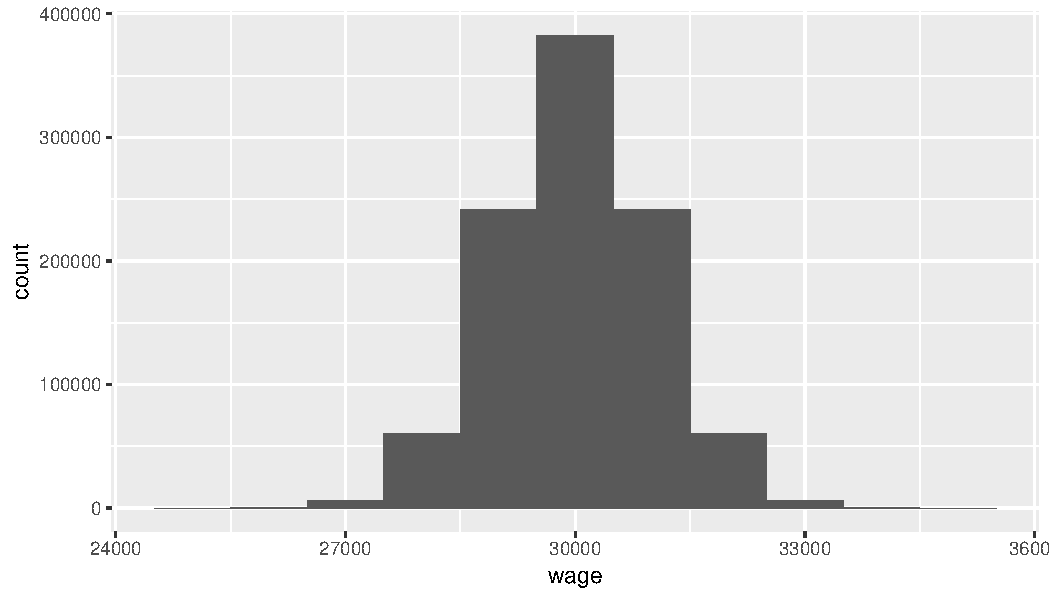
\includegraphics[width=\maxwidth]{figure/histbin1-1} 

}

\caption[A histogram of wages with bin size 1000]{A histogram of wages with bin size 1000.}\label{fig:histbin1}
\end{figure}


\end{knitrout}

\begin{knitrout}
\definecolor{shadecolor}{rgb}{0.969, 0.969, 0.969}\color{fgcolor}\begin{figure}

{\centering 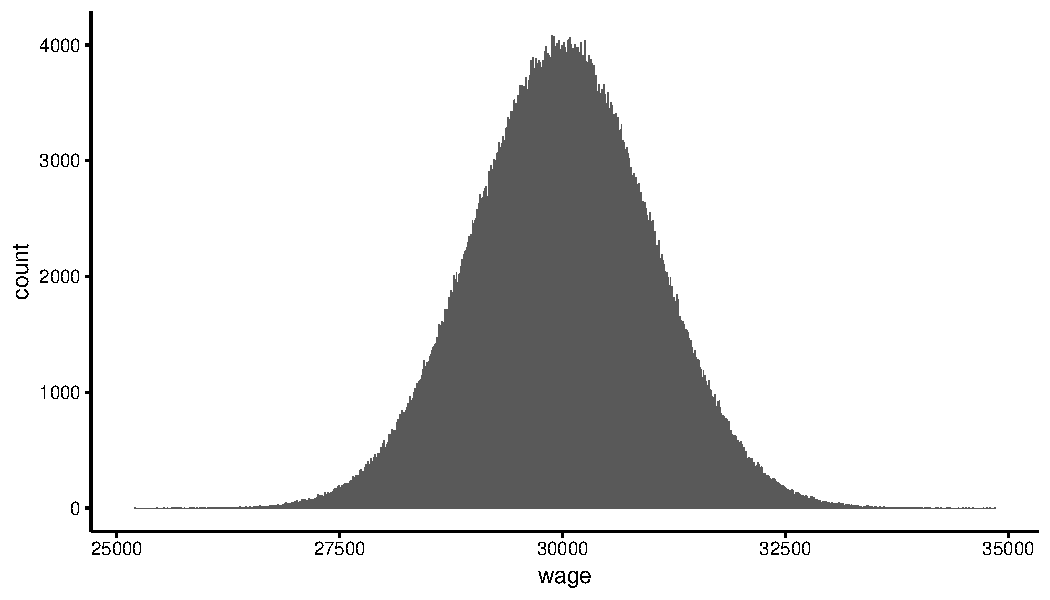
\includegraphics[width=\maxwidth]{figure/histbin2-1} 

}

\caption[A histogram of wages with bin size 10]{A histogram of wages with bin size 10.}\label{fig:histbin2}
\end{figure}


\end{knitrout}

The shape of the distribution that we discern in Figure \ref{fig:histbin2} can be represented by a \textit{density plot}. Density plots are an elegant representation of how the frequency of certain values are distributed across a continuum. They are particularly suited for large amounts of non-discrete (continuous) values, typically more than 1000. Figure \ref{fig:densitywages} shows a density plot of the one million wages. They more or less 'smooth' the histogram: drawing a smooth line connecting the dots of the histogram in Figure \ref{fig:histbin2} while looking through your eyelashes. On the vertical axis, we no longer see 'count' or 'frequency', but 'density'. The quantity \textit{density} is defined such that the area under the curve equals 1. Density plots are particularly suited for large data sets, where one is no longer interested in the particular counts, but  more interested in relative frequencies: how often are certain values observed, relative to other values. From this density plot, it is very clear that, relatively speaking, there are more values around 30,000 than around 27,500 or 32,500.

\begin{knitrout}
\definecolor{shadecolor}{rgb}{0.969, 0.969, 0.969}\color{fgcolor}\begin{figure}

{\centering 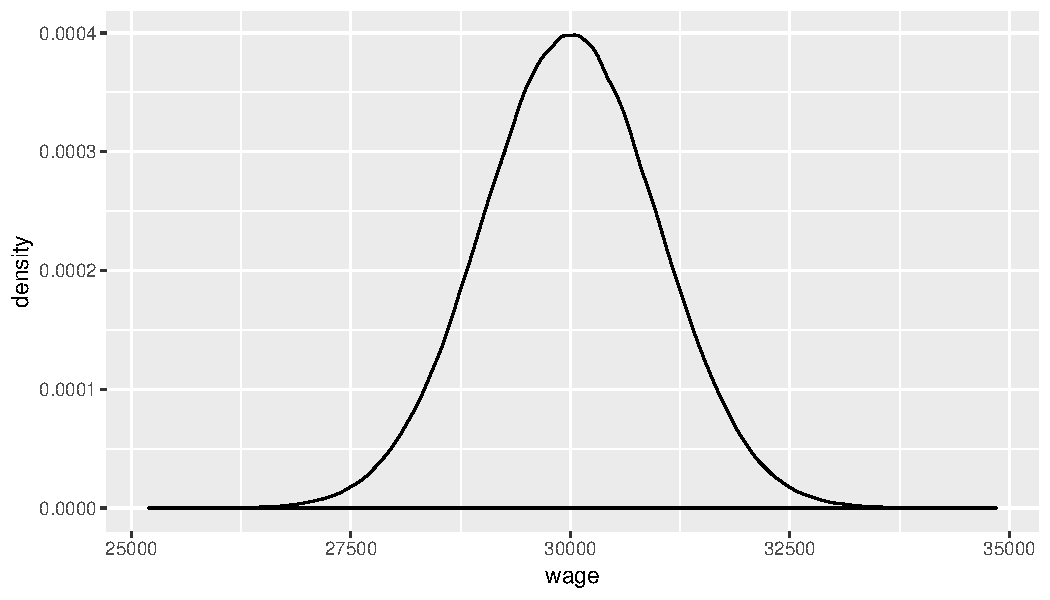
\includegraphics[width=\maxwidth]{figure/densitywages-1} 

}

\caption[A density plot of the wage variable]{A density plot of the wage variable.}\label{fig:densitywages}
\end{figure}


\end{knitrout}





% Figure \ref{fig:distr_3} shows a density plot of 1000 temperature values between 50 and 60 Fahrenheit, where all values had a precision of 4 decimal points (i.e., values like 53.9845, 56.0912, etc.). The plot suggests that values around 55 degrees are most frequent, and that values around 52 or around 58 are rather infrequent in the data set. On the vertical axis, we no longer see 'count' or 'frequency', but we see 'density'. Density is defined such that the area under the curve equals 1. Density plots are particularly suited for large data sets, where one is no longer interested in the particular counts: we're more interested in relative frequencies: how often are certain values observed, relative to other values. From this density plot, it is very clear that, relatively speaking, there are more values between 54 and 55 than between 52 and 53.
% 
% <<distr_3, fig.height=4, echo=FALSE, fig.align='center', message=F,warning=FALSE, fig.cap='Density plot of 1000 observed temperature measures.' >>=
% set.seed(1234)
%  tibble(temperature = rnorm(1000,55, 1)) %>%
%         ggplot(aes(temperature)) + geom_density()  +
%         scale_x_continuous(breaks=seq(50, 60)) +
%         xlim(c(50,60))
% @

\section{Density plots in R}

Density plots can be obtained using \texttt{geom\_density()}:

\begin{knitrout}
\definecolor{shadecolor}{rgb}{0.969, 0.969, 0.969}\color{fgcolor}\begin{kframe}
\begin{alltt}
\hlstd{mtcars} \hlopt
  \hlkwd{ggplot}\hlstd{(}\hlkwd{aes}\hlstd{(}\hlkwc{x} \hlstd{= mpg))} \hlopt{+}
  \hlkwd{geom_density}\hlstd{()}
\end{alltt}
\end{kframe}
\end{knitrout}


\section{The normal distribution}\label{sec:normal}

Sometimes distributions of observed variables bear close resemblance to \textit{theoretical} distributions. For instance, Figure \ref{fig:densitywages} bears close resemblance to the theoretical \textit{normal} distribution with mean 30,000 and standard deviation 1000. This theoretical shape can be described with the mathematical function

\begin{equation}
f(x)  = \frac{1}{\sqrt{2 \pi 1000^2}} e^{ { -\frac{(x - 30000)^2}{2 \times  1000^2}  } }
\end{equation}

which you are allowed to forget immediately. It is only to illustrate that distributions observed in the wild (empirical distributions) sometimes resemble mathematical functions (theoretical distributions).

The density function of that distribution is plotted in Figure \ref{fig:distr_4}. Because of its bell-shaped form, the normal distribution is sometimes informally called 'the bell curve'. The histogram in Figure \ref{fig:densitywages} and the normal density function in Figure \ref{fig:distr_4} look so similar, they are practically indistinguishable.





\begin{knitrout}
\definecolor{shadecolor}{rgb}{0.969, 0.969, 0.969}\color{fgcolor}\begin{figure}

{\centering 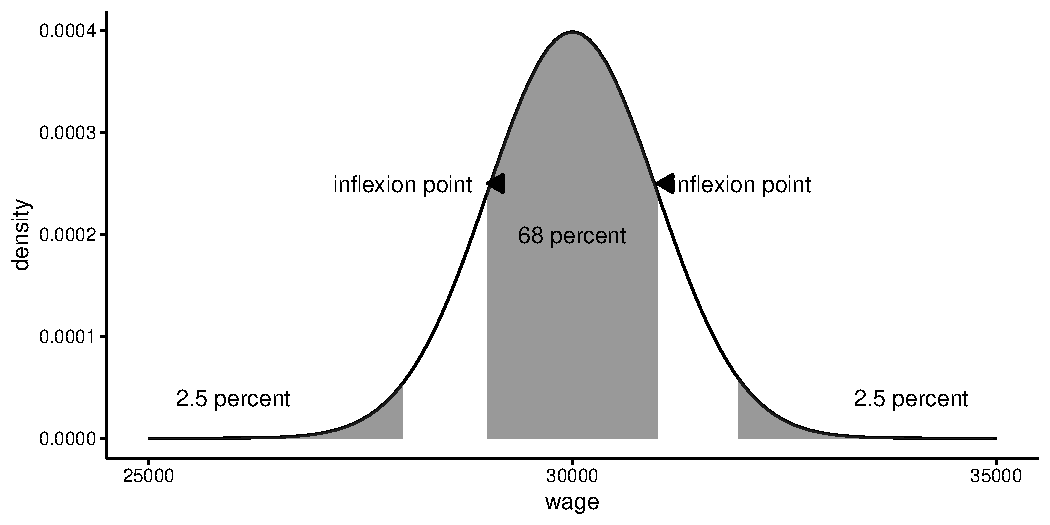
\includegraphics[width=\maxwidth]{figure/distr_4-1} 

}

\caption[The theoretical normal distribution with mean 30,000 and standard deviation 1000]{The theoretical normal distribution with mean 30,000 and standard deviation 1000.}\label{fig:distr_4}
\end{figure}


\end{knitrout}


Mathematicians have discovered many interesting things about the normal distribution. If the distribution of a variable closely resembles the normal distribution, you can infer many things. One thing we know about the normal distribution is that the mean, mode and median are always the same. Another thing we know from theory is that the inflexion points\footnote{The inflexion point is where concave turns into convex, and vice versa. Mathematically, the inflexion point can be found by equating the second derivative of a function to 0.} are one standard deviation away from the mean. Figure \ref{fig:distr_4} shows the two inflexion points. From theory we also know that if a variable has a normal distribution, 68\% of the observed values lies between these two inflexion points. We also know that 5\% of the observed values lie more than 1.96 standard deviations away from the mean (2.5\% on both sides, see Figure \ref{fig:distr_4}). Theorists have constructed tables that make it easy to see what proportion of values lies more than $1, 1.1, 1.2 \dots, 3.8, 3.9, \dots$ standard deviations away from the mean. These tables are easy to find online or in books, and these are fully integrated into statistical software like SPSS and R. Because all these percentages are known for the number of standard deviations, it is easier to talk about the \textit{standard normal distribution}.

In such tables online or in books, you find information only about this standard normal distribution. The standard normal distribution is a normal distribution where all values have been \textit{standardised} (see Section \ref{sec:standarddeviation}). When values have been standardised, they automatically have a mean of 0 and a standard deviation of 1. As we saw in Section \ref{sec:standarddeviation}, such standardised values are obtained if you subtract the mean score from each value, and divide the result by the standard deviation. A standardised value is usually denoted as a $z$-score. Thus in formula form, a value $Y=y$ is standardised by using the following equation:


\begin{equation}
z = \frac{y - \widebar{Y}}{\sigma}
\end{equation}



% latex table generated in R 4.0.3 by xtable 1.8-4 package
% Sun Jan 31 16:36:30 2021
\begin{table}[ht]
\centering
\caption{Standardising scores.} 
\label{tab:normal_1}
\begin{tabular}{rrrr}
  \hline
Y & mean & Y\_minus\_mean & Z \\ 
  \hline
7.2 & 10.4 & -3.2 & -0.7 \\ 
  8.8 & 10.4 & -1.5 & -0.3 \\ 
  17.8 & 10.4 & 7.4 & 1.6 \\ 
  10.4 & 10.4 & -0.0 & -0.0 \\ 
  10.6 & 10.4 & 0.3 & 0.1 \\ 
  18.6 & 10.4 & 8.2 & 1.7 \\ 
  12.3 & 10.4 & 1.9 & 0.4 \\ 
  3.7 & 10.4 & -6.7 & -1.4 \\ 
  6.6 & 10.4 & -3.8 & -0.8 \\ 
  7.8 & 10.4 & -2.6 & -0.5 \\ 
   \hline
\end{tabular}
\end{table}


Table \ref{tab:normal_1} shows an example set of values for $Y$ that are standardised. The mean of the $Y$-values turns out to be 10.38, and the standard deviation 4.77. By subtracting the mean, we ensure that the average $z$-score becomes 0, and by subsequently dividing by the standard deviation, we make sure that the standard deviation of the $z$-scores becomes 1.

This standardisation makes it much easier to look up certain facts about the normal distribution. For instance, if we go back to the normally distributed wage values, we see that the average is 30,000, and the standard deviation is 1,000. Thus, if we take all wages, subtract 30,000 and divide by 1,000, we get standardised wages with mean 0 and standard deviation 1. The result is shown in Figure \ref{fig:normal_2}. We know that the inflexion points lie at one standard deviation below and above the mean. The mean is 30,000, and the standard deviation equals 1,000, so the inflexion points are at $30000-1000=29000$ and $30000+1000=31000$. Thus we know that 68\% of the wages are between 29,000 and 31,000.


\begin{knitrout}
\definecolor{shadecolor}{rgb}{0.969, 0.969, 0.969}\color{fgcolor}\begin{figure}

{\centering 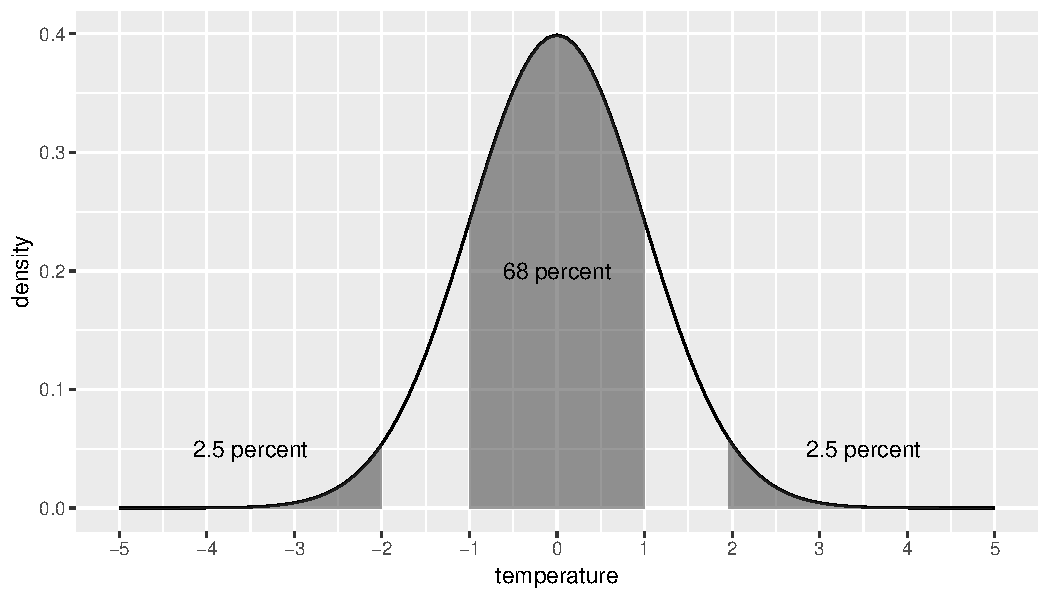
\includegraphics[width=\maxwidth]{figure/normal_2-1} 

}

\caption[The standard normal distribution]{The standard normal distribution.}\label{fig:normal_2}
\end{figure}


\end{knitrout}



How do we know that 68\% of the observations lie between the two inflexion points? Similar to proportions and cumulative proportions, we can plot the cumulative normal distribution. Figure \ref{fig:normal_3} shows the cumulative proportions curve for the normal distribution. Note that we no longer see dots because the variable $Z$ is continuous.

\begin{knitrout}
\definecolor{shadecolor}{rgb}{0.969, 0.969, 0.969}\color{fgcolor}\begin{figure}

{\centering 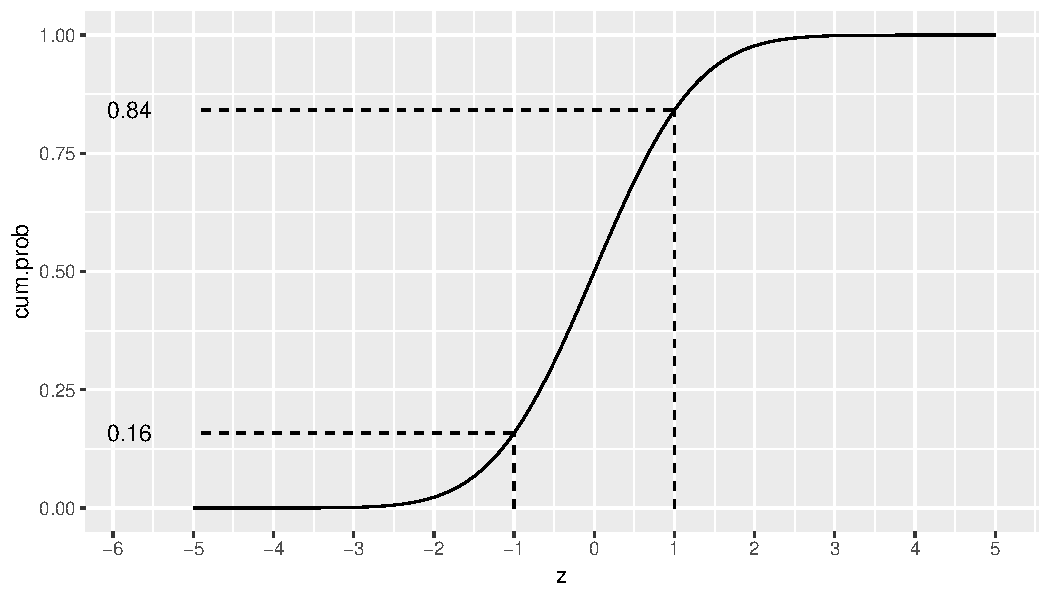
\includegraphics[width=\maxwidth]{figure/normal_3-1} 

}

\caption[The cumulative standard normal distribution]{The cumulative standard normal distribution.}\label{fig:normal_3}
\end{figure}


\end{knitrout}

We know that the two inflexion points lie one standard deviation below and above the mean. Thus, if we look at a $z$-value of 1, we see that the cumulative probability equals about 0.84. This means that 84\% of the $z$-values are lower than 1. If we look at a $z$-value of -1, we see that the cumulative probability equals about 0.16. This means that 16\% of the $z$-values are lower than -1. Therefore, if we want to know what percentage of the $z$-values lie between -1 and 1, we can calculate this by subtracting 0.16 from 0.84, which equals 0.68, which corresponds to 68\%.

All quantiles for the standard normal distribution can be looked up online\footnote{See for example www.normaltable.com or www.mathsisfun.com/data/standard-normal-distribution-table.html} or in Appendix \ref{app:normal}, but also using R. Table \ref{tab:normal_4} gives a short list of quantiles. From this table, you see that 1\% of the $z$-values is lower than -2.33, and that 25\% of the $z$-values is lower than -0.67. We also see that half of all the $z$-values is lower than 0.00 and that 10\% of the $z$-values is larger than 1.28, and that the 1\% largest values are higher than 2.33. 

Although tables are readily found online, it's helpful to memorise the so-called \textit{68 --  95 -- 99.7 rule}, also called \textit{the empirical rule}. It says that 68\% of normally distributed values are at most 1 standard deviation away from the mean, 95\% of the values are at most 2 standard deviations away (more precisely, 1.96), and 99.7\% of the values are at most 3 standard deviations away. In other words, 68\% of standardised values are between -1 and +1, 95\% of standardised values are between -2 and +2 (-1.96 and +1.96), and 99.7\% of standardised values are between -3 and +3.

% latex table generated in R 4.0.3 by xtable 1.8-4 package
% Sun Jan 31 16:36:31 2021
\begin{table}[ht]
\centering
\caption{Some quantiles for the standard normal distribution.} 
\label{tab:normal_4}
\begin{tabular}{rr}
  \hline
Z & cum\_proportion \\ 
  \hline
-2.33 & 0.01 \\ 
  -1.28 & 0.10 \\ 
  -0.67 & 0.25 \\ 
  0.00 & 0.50 \\ 
  0.67 & 0.75 \\ 
  1.28 & 0.90 \\ 
  2.33 & 0.99 \\ 
   \hline
\end{tabular}
\end{table}



Thus, if we return to our wages with mean 30,000 and standard deviation 1,000, we know from Table \ref{tab:normal_4} that 99\% of the wages are below 30000 + 2.33 times the standard deviation = $30000 + 2.33 \times 1000=32330$.

Returning back to the IQ example of Section \ref{sec:standarddeviation}. Suppose we have IQ scores that are normally distributed with a mean of 100 and a standard deviation of 15. What IQ score would be the 90th percentile? From Table \ref{tab:normal_4} we see that the 90th percentile is a $z$-value of 1.28. Thus, the 90th percentile for our IQ scores lies 1.28 standard deviations above the mean (above because the $z$-value is positive). The mean is 100 so we have to look at 1.28 standard deviations above that. The standard deviation equals 15, so we have to look at an IQ score of $100 + 1.28 \times 15$, which equals 119.2. This tells us that 90\% of the IQ scores are equal to or lower than 119.2.

As a last example, suppose we have a personality test that measures extraversion. If we know that test scores are normally distributed with a mean of 18 and a standard deviation of 2, what would be the 0.10 quantile? From Table \ref{tab:normal_4} we see that the 0.10 quantile is a $z$-value of -1.28. This tells us that the 0.10 quantile for the personality scores lies at 1.28 standard deviations below the mean. The mean is 18, so the 0.10 quantile for the personality scores lies at 1.28 standard deviations below 18. The standard deviation is 2, so this amounts to $18-1.28 \times 2= 15.44$. This tells us that 10\% of the scores on this test are 15.44 or lower.

Such handy tables are also available for other theoretical distributions. Theoretical distributions are at the core of many data analysis techniques, including linear models. In this book, apart from the normal distribution, we will also encounter other theoretical distributions: the $t$-distribution (Chapter \ref{chap:mean}), the $F$-distribution (Chapter \ref{chap:categorical}), the chi-square distribution (Chapters \ref{chap:mean}, \ref{chap:nonpar1}, \ref{chap:nonpar2}, \ref{chap:logistic} and \ref{chap:poisson}) and the Poisson distribution (\ref{chap:poisson}).

% \subsection{The chi-square distribution}
% Suppose that we have 1,000 temperature measures from one location. Say that these measures were taken on 1000 different days, so that for each day, temperature was measured once randomly during the day. If we compute, for every day, the squared deviation of the observed temperature from the average temperature, and we plot these 1000 different values, we might get something like is shown in Figure \ref{fig:distr_5}. This in turn bears close resemblance to another theoretical distributution, the chi-square distibution (or $\chi^2$-distribution). This $\chi^2$-distribution is plotted in Figure \ref{fig:distr_6}. For this distribution, there are also tables that tell us the percentage of observed values that are equal to or smaller than a particular value, say 5. For example, we know from theory that for the chi-square distribution depicted in Figure \ref{fig:distr_5}, that 95\% of the values is smaller than 3.84.
% 
% <<distr_5, fig.height=4, echo=T, fig.align='center', warning=T, fig.cap='Density plots of 1000 observed squared deviations from the average temperature.' >>=
% set.seed(1234)
% tibble(temperature = rnorm(1000,30000, 1), day=rep(1:1000)) %>%
%         group_by(day) %>%
%         summarise(SS=(temperature-30000)^2) %>%
%         ggplot()+
%         geom_density(aes(x=SS)) +
%         ylab("density") + xlab("Temperature minus average temperature squared")+
%         xlim(c(0,10))
% @
% %
% 
% %%%% something goes wrong when running with this figure below that didnt go wrong before. something to doe with \vref or \vpageref (may loop) package varioref error
% 
% 
% <<distr_6, fig.height=2, echo=T, message=T, fig.align='center', warning=T, fig.cap='The theoretical chi-square distribution' >>=
% shaded <-  tibble(x = seq(3.84, 10,0.1),  y = dchisq(seq(3.84, 10,0.1), 1, 0))
% tibble(temperature = seq(0.18,10,0.1)) %>%
%         ggplot()+
%         geom_line(aes(x=temperature, y = dchisq(temperature,df=1, ncp=0))) +
%         geom_area(data=shaded, mapping = aes(x=x ,  y=y),alpha=0.5)+
%         ylab("density") + xlab("chi-square")
%         xlim(c(0,10)) +
%         geom_text(x=3.84,y=-0.01, label=paste(3.84))+
%           geom_text(x=5.5, y=0.05, label="5 percent")
%  @
% %
%


\section{Obtaining quantiles of the normal distribution using R}

Quantiles of a normal distribution with a certain mean and standard deviation (sd) can be obtained using the \texttt{qnorm()} function:

\begin{knitrout}
\definecolor{shadecolor}{rgb}{0.969, 0.969, 0.969}\color{fgcolor}\begin{kframe}
\begin{alltt}
\hlkwd{qnorm}\hlstd{(}\hlkwd{c}\hlstd{(}\hlnum{0.05}\hlstd{,} \hlnum{0.50}\hlstd{,} \hlnum{0.95}\hlstd{),} \hlkwc{mean} \hlstd{=} \hlnum{100}\hlstd{,} \hlkwc{sd} \hlstd{=} \hlnum{15}\hlstd{)}
\end{alltt}
\begin{verbatim}
## [1]  75.3272 100.0000 124.6728
\end{verbatim}
\end{kframe}
\end{knitrout}

This means that if you have a normal distribution with mean 100 and standard deviation 15, 5\% of the values are 75.3272 or less, 50\% of the values are 100 or less, and 95\% of the values are 124.6728 or less.

If you want to know the cumulative proportion for a certain value of a variable that is normally distributed, you can use \texttt{pnorm()}:

\begin{knitrout}
\definecolor{shadecolor}{rgb}{0.969, 0.969, 0.969}\color{fgcolor}\begin{kframe}
\begin{alltt}
\hlkwd{pnorm}\hlstd{(}\hlopt{-}\hlnum{1}\hlstd{,} \hlkwc{mean} \hlstd{=} \hlnum{0}\hlstd{,} \hlkwc{sd} \hlstd{=} \hlnum{1}\hlstd{)}
\end{alltt}
\begin{verbatim}
## [1] 0.1586553
\end{verbatim}
\end{kframe}
\end{knitrout}

So 15.86\% of the values from a standard normal distribution (mean 0, standard deviation 1), are -1 or less.

\section{Visualising numeric variables: the box plot}

We started this chapter with variables that can be stored in a data matrix. With a variable with a large number of values on a large number of units of analysis, it is hard to get a an intuitive feel for the data. Making a frequency table is one way of summarising a variable, computing measures of central tendency and variation is another way. Visualisation is probably the best way of getting a quick and dirty feel for the information contained in a large data matrix. Earlier in this chapter we came across frequency plots, histograms, and density plots to visualise the distribution of a single variable. A fourth plot for a single variable that we discuss in this book is the \textit{box plot}.  

A box plot gives a quick overview of the distribution of a numeric variable in terms of its quartiles. Figure \ref{fig:chis_7} gives an example of a box plot of (part of) the wage data. The white box represents the interquartile range. The top of the white box equals the third quartile, and the bottom of the white box equals the first quartile. Therefore, we know that half of the workers have a wage between 29,400 and 30,800 The horizontal black line within the white box represents the second quartile (the median), so half of the workers earn less than 30,100. 

A box plot also shows whiskers: two vertical lines sprouting from the white box. There are several ways to draw these two whiskers. One way is to draw the top whisker to the largest value (the maximum) and the bottom whisker to the smallest value (the minimum). Another way, used in Figure \ref{fig:chis_7}, is to have the upper whisker extend from the third quartile to the observed value equal to at most 1.5 times the interquartile range away from the median, and the lower whisker extend from the first quartile to the value at most 1.5 times the interquartile range below the median (the interquartile range is of course the height of the white box). The dots are outlying values, or simply called \textit{outliers}: values that are even further away from the median. This is displayed in Figure \ref{fig:chis_7}. There you see first and third quartiles of 29,400 and 30,800, respectively, so an interquartile range (IQR) of $30800-29400=1400$. Multiplying this IQR by 1.5 we get $1.5 \times 1400= 2100$. The whiskers therefore extend to $29400-2100=27300$ and $30800+2100=32900$. 

Thus, the box plot is a quick way of visualising in what range the middle half of the values are (the range in the white box), where most of the values are (the range of the white box plus the whiskers), and where the extreme values are (the outliers, individually plotted as dots). Note that the white box always contains 50\% of the values. The whiskers are only extensions of the box by a factor of 1.5. In many cases you see that they contain most of the values, but sometimes they miss a lot of values. You will see that when you notice a lot of outliers.

\begin{knitrout}
\definecolor{shadecolor}{rgb}{0.969, 0.969, 0.969}\color{fgcolor}\begin{figure}

{\centering 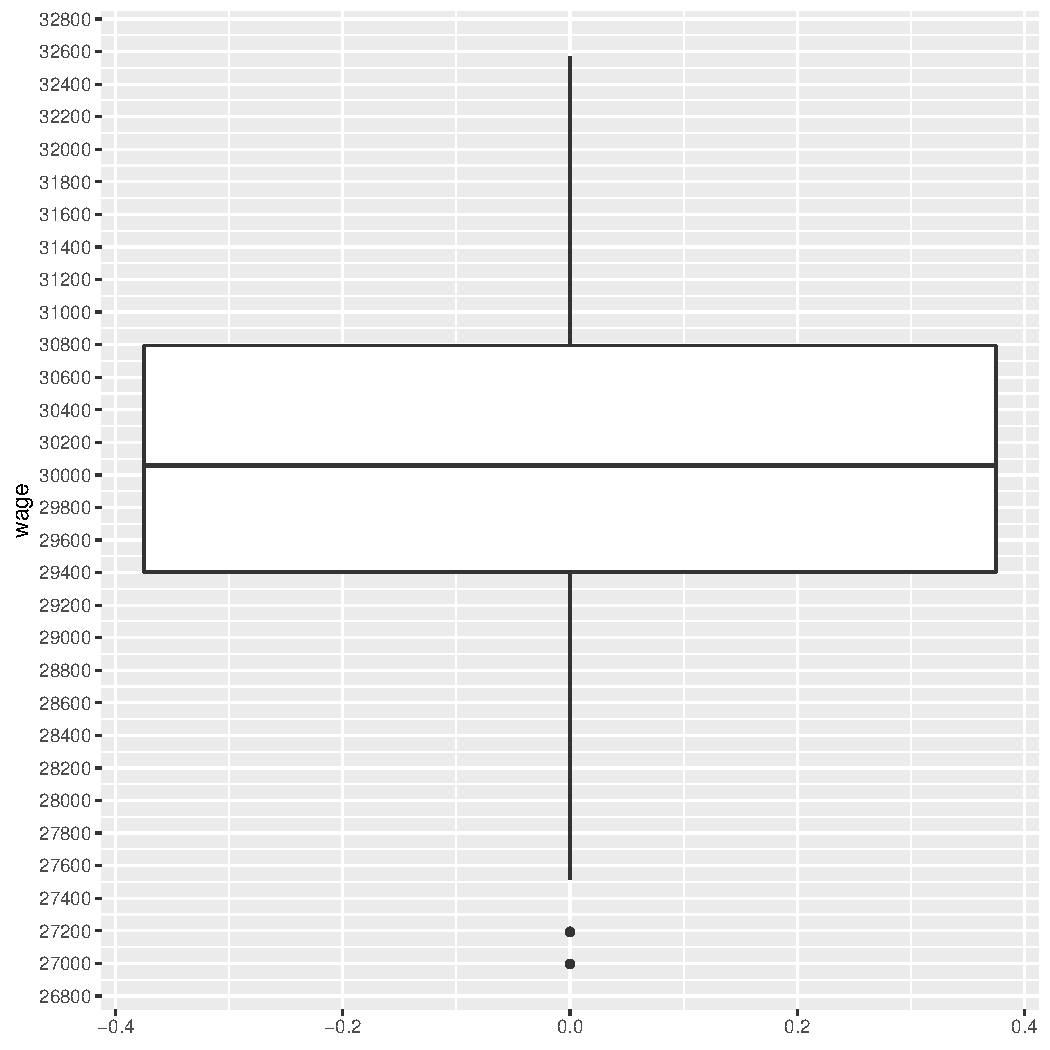
\includegraphics[width=\maxwidth]{figure/chis_7-1} 

}

\caption[A box plot of the wages earned by a sample of 150 administrative clerks]{A box plot of the wages earned by a sample of 150 administrative clerks}\label{fig:chis_7}
\end{figure}


\end{knitrout}

\section{Box plots in R}

A box plot can be made using \texttt{geom\_boxplot()}:

\begin{knitrout}
\definecolor{shadecolor}{rgb}{0.969, 0.969, 0.969}\color{fgcolor}\begin{kframe}
\begin{alltt}
\hlstd{mtcars} \hlopt
  \hlkwd{ggplot}\hlstd{(}\hlkwd{aes}\hlstd{(}\hlkwc{x} \hlstd{=} \hlstr{""}\hlstd{,} \hlkwc{y} \hlstd{= mpg))} \hlopt{+}
  \hlkwd{geom_boxplot}\hlstd{()} \hlopt{+}
  \hlkwd{xlab}\hlstd{(}\hlstr{""}\hlstd{)}
\end{alltt}
\end{kframe}
\end{knitrout}



\section{Visualising categorical variables}

The histogram, the density plot and the box plot can be used for numeric variables, but also for ordinal variables that you'd like to treat numerically. For categorical variables and ordinal variables that can't be treated numerically, we need other types of plots.

For example, suppose we are in a lecture hall with 456 students and we count the number of Dutch, German, Belgian, Indian, Chinese and Indonesian students. We could summarise the results in a frequency table (see Table \ref{tab:nationality_1}), but a \textit{bar chart} shows the distribution in a more dramatic way, see Figure \ref{fig:nationality_2}.



% latex table generated in R 4.0.3 by xtable 1.8-4 package
% Sun Jan 31 16:36:31 2021
\begin{table}[ht]
\centering
\caption{A frequency table of nationalities.} 
\label{tab:nationality_1}
\begin{tabular}{lr}
  \hline
nationality & n \\ 
  \hline
Chinese & 10 \\ 
  Dutch & 145 \\ 
  German & 284 \\ 
  Indian & 7 \\ 
  Indonesian & 10 \\ 
   \hline
\end{tabular}
\end{table}


\begin{knitrout}
\definecolor{shadecolor}{rgb}{0.969, 0.969, 0.969}\color{fgcolor}\begin{figure}

{\centering 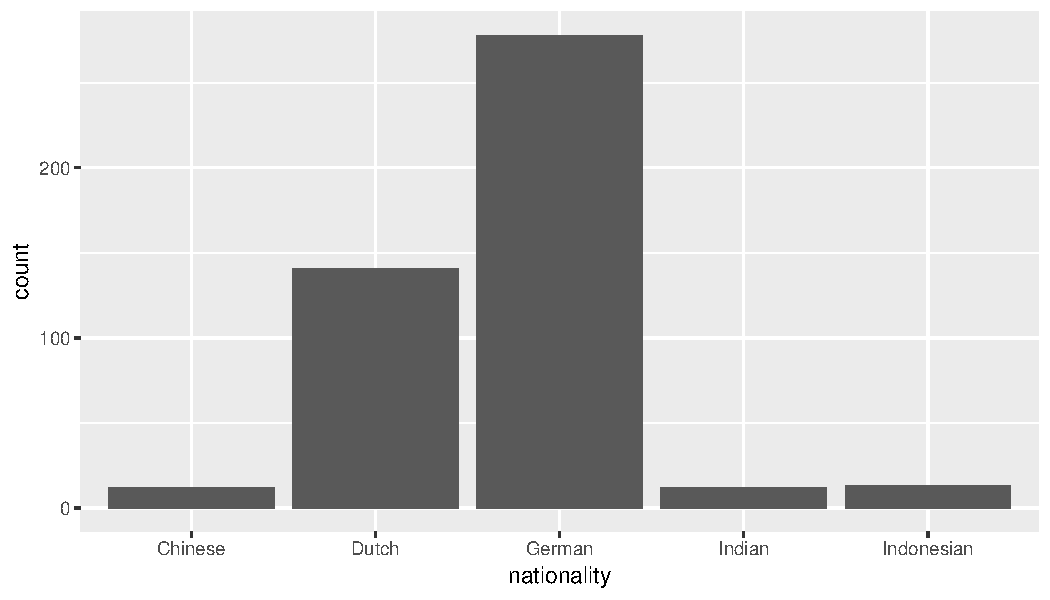
\includegraphics[width=\maxwidth]{figure/nationality_2-1} 

}

\caption[A bar chart of the observed nationalities in a lecture hall]{A bar chart of the observed nationalities in a lecture hall.}\label{fig:nationality_2}
\end{figure}


\end{knitrout}

Sometimes, counts of values of a categorical variable are displayed as a \textit{pie chart}, see Figure \ref{fig:nationality_3}. Pie charts are however best avoided. First, because compared to bar charts, they show no information about the actual counts; you only observe relative sizes of the counts. Second, it is very hard to see from a pie chart what the exact proportions are. For example, from the bar chart in Figure \ref{fig:nationality_2} it is easily seen that the ratio German students to Dutch students is about 2 to 1. Research shows that this ratio cannot be read with the same precision from the pie chart in Figure \ref{fig:nationality_3}. In sum, pie charts are best replaced by bar charts.



\begin{knitrout}
\definecolor{shadecolor}{rgb}{0.969, 0.969, 0.969}\color{fgcolor}\begin{figure}

{\centering 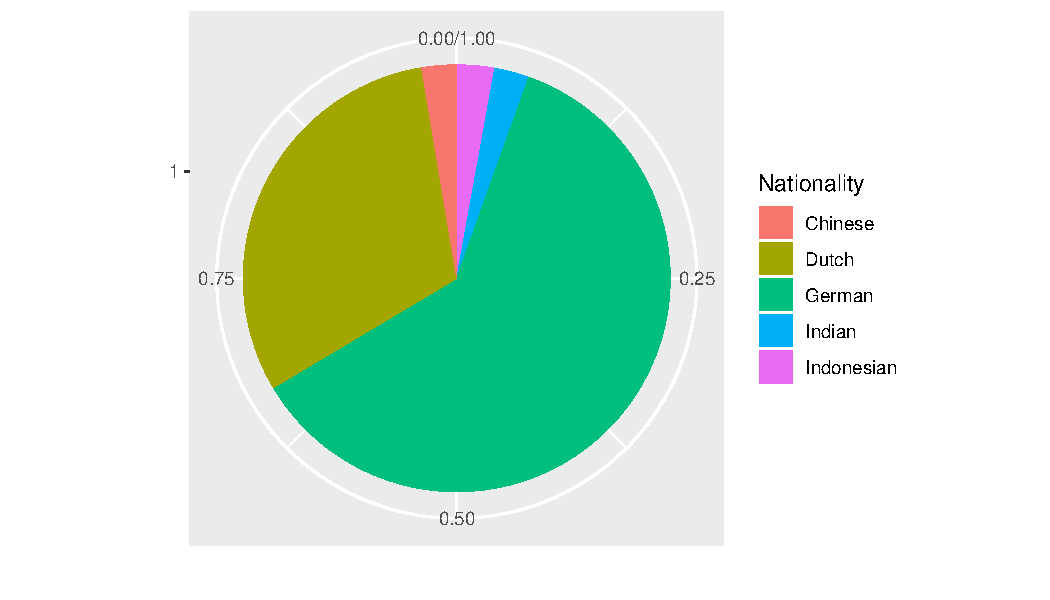
\includegraphics[width=\maxwidth]{figure/nationality_3-1} 

}

\caption[A pie chart of nationalities]{A pie chart of nationalities.}\label{fig:nationality_3}
\end{figure}


\end{knitrout}


Ordinal variables are often visualised using bar charts. Figure \ref{fig:climate_1} shows the variation of the answers to a Likert questionnaire item, where Nairobi inhabitants are asked "To what degree do you agree with the statement that the climate in Iceland is agreeable?". With ordinal variables, make sure that the labels are in the natural order. 

\begin{figure}

{\centering 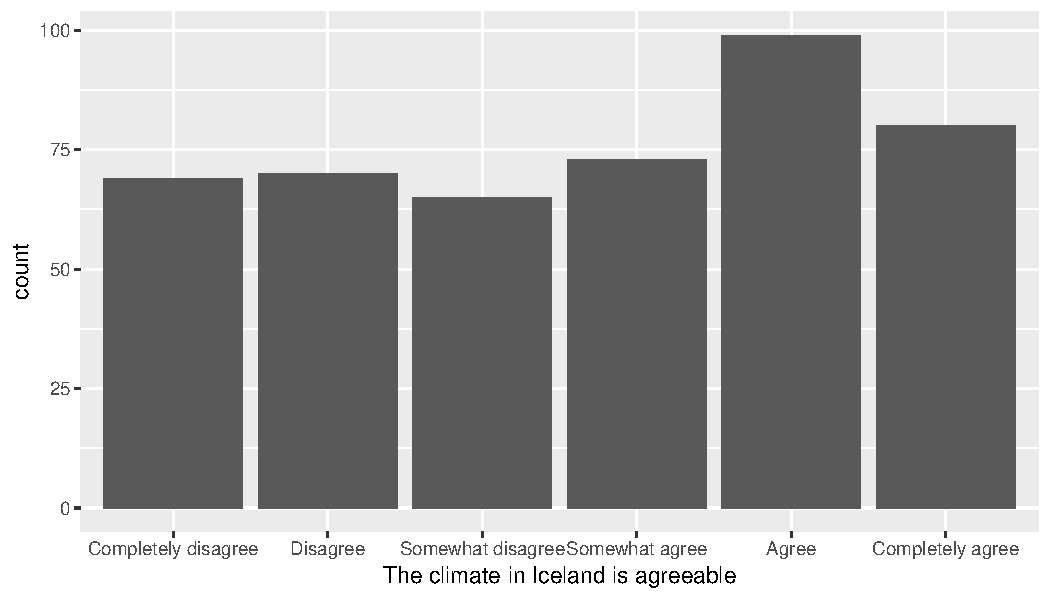
\includegraphics[width=\maxwidth]{figure/climate_1-1} 

}

\caption[Opinions on the climate in Iceland]{Opinions on the climate in Iceland.}\label{fig:climate_1}
\end{figure}




\section{Visualising categorical and ordinal variables in R}

If a categorical variable is stored as numeric, turn it into a factor first. Then R will treat it as categorical. A bar plot with the frequencies on the $y$-axis can be made with \texttt{geom\_bar()}: 

\begin{knitrout}
\definecolor{shadecolor}{rgb}{0.969, 0.969, 0.969}\color{fgcolor}\begin{kframe}
\begin{alltt}
\hlstd{mtcars} \hlopt
  \hlkwd{mutate}\hlstd{(}\hlkwc{cyl} \hlstd{=} \hlkwd{factor}\hlstd{(cyl,} \hlkwc{ordered} \hlstd{=} \hlnum{TRUE}\hlstd{))} \hlopt
  \hlkwd{ggplot}\hlstd{(}\hlkwd{aes}\hlstd{(}\hlkwc{x} \hlstd{= cyl))} \hlopt{+}
  \hlkwd{geom_bar}\hlstd{()}
\end{alltt}
\end{kframe}
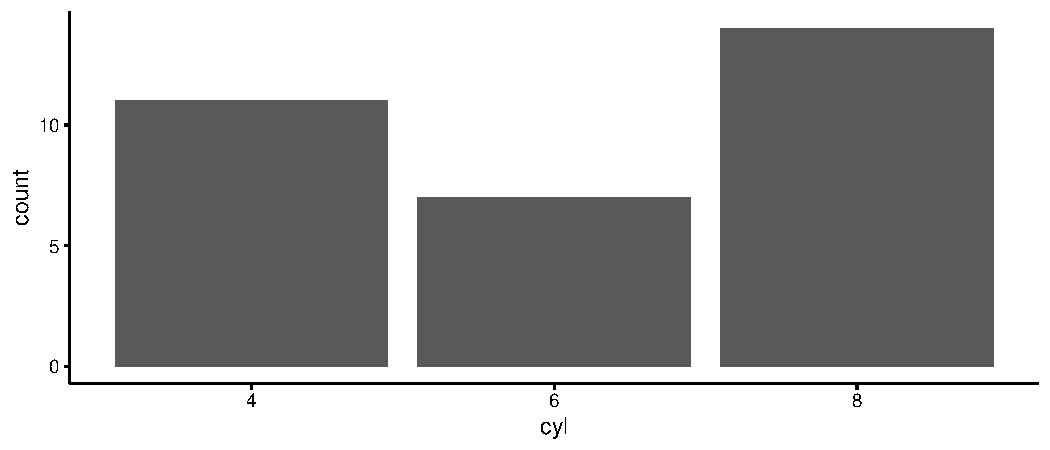
\includegraphics[width=\maxwidth]{figure/unnamed-chunk-31-1} 

\end{knitrout}

If you really want a pie chart, then do:

\begin{knitrout}
\definecolor{shadecolor}{rgb}{0.969, 0.969, 0.969}\color{fgcolor}\begin{kframe}
\begin{alltt}
\hlstd{mtcars} \hlopt
  \hlkwd{count}\hlstd{(cyl)} \hlopt
  \hlkwd{mutate}\hlstd{(}\hlkwc{proportion} \hlstd{= n}\hlopt{/}\hlkwd{sum}\hlstd{(n))} \hlopt
  \hlkwd{ggplot}\hlstd{(}\hlkwd{aes}\hlstd{(}\hlkwc{x} \hlstd{=} \hlstr{""}\hlstd{,}
             \hlkwc{y} \hlstd{= proportion,}
             \hlkwc{fill} \hlstd{=} \hlkwd{factor}\hlstd{(cyl)))} \hlopt{+}
  \hlkwd{geom_col}\hlstd{(}\hlkwc{width} \hlstd{=} \hlnum{1}\hlstd{)} \hlopt{+}
  \hlkwd{coord_polar}\hlstd{(}\hlkwc{theta} \hlstd{=} \hlstr{"y"}\hlstd{)} \hlopt{+}
  \hlkwd{xlab}\hlstd{(}\hlstr{""}\hlstd{)} \hlopt{+}
  \hlkwd{ylab}\hlstd{(}\hlstr{""}\hlstd{)} \hlopt{+}
  \hlkwd{theme_void}\hlstd{()} \hlopt{+}
  \hlkwd{scale_fill_brewer}\hlstd{(}\hlkwc{palette} \hlstd{=} \hlstr{"Blues"}\hlstd{)} \hlopt{+}
  \hlkwd{labs}\hlstd{(}\hlkwc{fill} \hlstd{=} \hlstr{"Cylinders"}\hlstd{)}
\end{alltt}
\end{kframe}
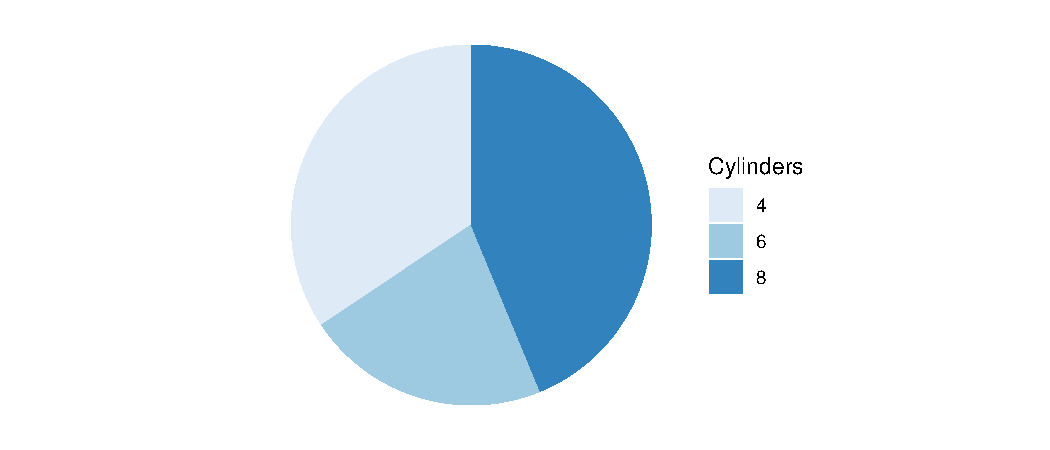
\includegraphics[width=\maxwidth]{figure/unnamed-chunk-32-1} 

\end{knitrout}


\section{Visualising co-varying variables}

\subsection{Categorical by categorical: cross-table}

Variables are properties that vary: from person to person, or from location to location, or from time to time, or from object to object. Sometimes when you have two variables, you see that they co-vary: when one variable changes, the other variable changes too. For example, suppose I have 20 pencils. These pencils may vary in colour: twelve of them are red, and eight of them are blue. Therefore, \texttt{colour} is a variable with values "red" and "blue". The twenty pencils also vary in length: four are unused and therefore still long, and sixteen of them have been used many times so that they are short. Therefore, \texttt{length} is also a variable, with values "long" and "short". Note that these variables have been measured using the same pencils. In theory I could have long blue pencils, long red pencils, short blue pencils and short red pencils. Let's look at the pencils that I have: for each combination of \texttt{length} and \texttt{colour}, I count the number of pencils. The result I put in Table \ref{tab:cross-table_1}.

% latex table generated in R 4.0.3 by xtable 1.8-4 package
% Sun Jan 31 16:36:32 2021
\begin{table}[ht]
\centering
\caption{Cross-tabulation of colour and length for twenty pencils.} 
\label{tab:cross-table_1}
\begin{tabular}{rrr}
  \hline
 & blue & red \\ 
  \hline
long & 4 & 0 \\ 
  short & 8 & 8 \\ 
   \hline
\end{tabular}
\end{table}


Such a table is called a \textit{cross-table}. For every combination of two variables, I see the number of objects (units of analysis) that have that combination. From the table we see that there is not a single pencil that is both red and long (count is 0). At the same time you see that all long pencils are blue. A cross-table is therefore a nice way to show how two variables co-vary. From this particular table for instance, you can easily see that once you know that a pencil is long, you automatically know it is blue.


Cross-tables are a nice visualisation of how two categorical variables co-vary. But what if one of the two variables is not a categorical variable?


\subsection{Categorical by numerical: box plot}
Suppose instead of determining length by values "short" and "long", we could measure the exact length of the pencils in centimetres. The results are displayed in Table \ref{tab:cross-table_2}. We see that the table is much larger than Table \ref{tab:cross-table_1}. We also see quite a few cells with zeros. In most cases, for every particular combination of length and colour we only see a count of 1 pencil. In general, you see that when one of the variables is numeric, the cross-table becomes very large and in addition it becomes sparse, that is, with many zeros. With such a large and sparse table, it is hard to get a quick impression of how two variables co-vary.

% latex table generated in R 4.0.3 by xtable 1.8-4 package
% Sun Jan 31 16:36:32 2021
\begin{table}[ht]
\centering
\caption{Cross-tabulation of colour and length for twenty pencils.} 
\label{tab:cross-table_2}
\begin{tabular}{rrr}
  \hline
 & blue & red \\ 
  \hline
2 &   0 &   1 \\ 
  2.7 &   1 &   0 \\ 
  3.3 &   1 &   0 \\ 
  3.4 &   0 &   1 \\ 
  3.5 &   0 &   1 \\ 
  3.6 &   1 &   0 \\ 
  4.1 &   1 &   1 \\ 
  4.4 &   1 &   1 \\ 
  4.5 &   1 &   1 \\ 
  4.7 &   0 &   1 \\ 
  5.2 &   1 &   0 \\ 
  5.7 &   1 &   0 \\ 
  5.8 &   0 &   1 \\ 
  9 &   4 &   0 \\ 
   \hline
\end{tabular}
\end{table}



The alternative for two variables where one is categorical and the other one is numeric, is to create a \textit{box plot}. Figure \ref{fig:crosstable_3} shows a box plot of the pencil data. A box plot gives a quick overview of the distribution of the pencils: one distribution of the blue pencils, and one distribution of the red pencils. Let's have a look at the distribution of the blue pencils on the left side of the plot. The white box represents the interquartile range (IQR), so that we know that half of the blue pencils have a length between 4 and 9. The horizontal black line within the white box represents the median (the middle value), so half of the blue pencils are smaller than 4.85. The vertical lines are called whiskers. These typically indicate where the data points are that lie at most 1.5 times the IQR away from the median. For the blue pencils, we see no whisker on top of the white box. That means that there are no data points that lie more than 1.5 times the IQR above the median of 4.85 (here the IQR equals 5.03). We see a whisker on the bottom of the white box, to the lowest observed value of 2.7. This value is less than 1.5 times $5.03 = 7.545$ away from the median of 4.85 so it is included in the whisker. It is the lowest observed value for the blue pencils so the whisker ends there. 


\begin{figure}

{\centering 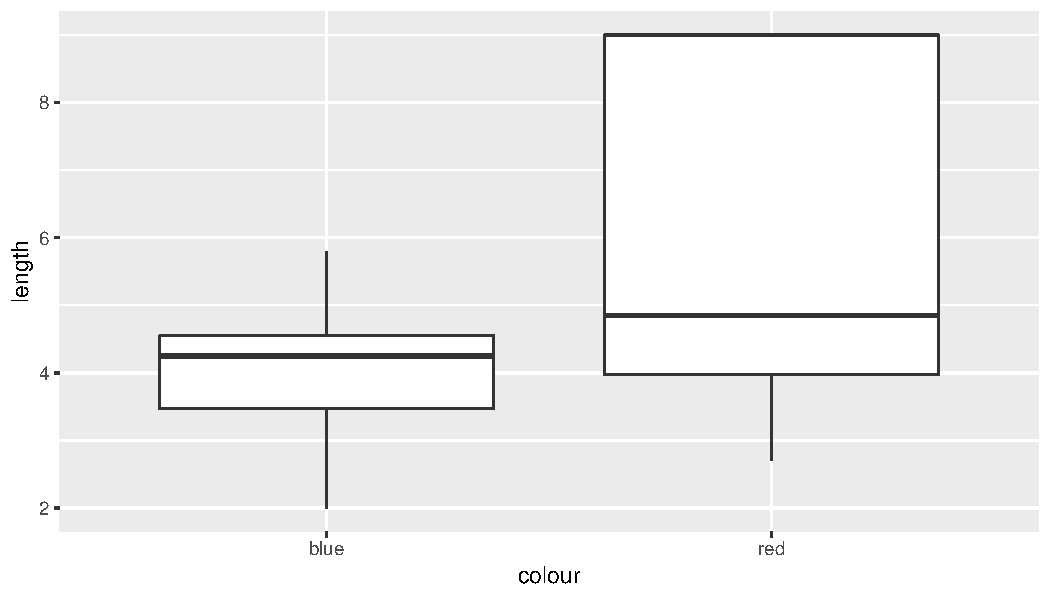
\includegraphics[width=\maxwidth]{figure/crosstable_3-1} 

}

\caption[A box plot of the pencil data]{A box plot of the pencil data.}\label{fig:crosstable_3}
\end{figure}



From a box plot like this it is easy to spot differences in the distribution of a quantitative measure for different levels of a qualitative measure. From Figure \ref{fig:crosstable_3} we easily spot that the red pencils (varying between 2 and 6 cm) tend to be shorter than the blue pencils (varying between 3 and 9 cm). Thus, in these pencils, \texttt{length} and \texttt{colour} tend to co-vary: red pencils are often short and blue pencils are often long.


\subsection{Numeric by numeric: scatter plot}

% latex table generated in R 4.0.3 by xtable 1.8-4 package
% Sun Jan 31 16:36:32 2021
\begin{table}[ht]
\centering
\caption{Cross-tabulation of length (rows) and weight (columns) for twenty pencils.} 
\label{tab:cross-table_4}
\begin{tabular}{rrrrrrr}
  \hline
 & 3.3 & 3.4 & 3.5 & 3.6 & 3.7 & 4 \\ 
  \hline
2 &   1 &   0 &   0 &   0 &   0 &   0 \\ 
  2.7 &   0 &   1 &   0 &   0 &   0 &   0 \\ 
  3.3 &   0 &   1 &   0 &   0 &   0 &   0 \\ 
  3.4 &   0 &   1 &   0 &   0 &   0 &   0 \\ 
  3.5 &   0 &   0 &   1 &   0 &   0 &   0 \\ 
  3.6 &   0 &   0 &   1 &   0 &   0 &   0 \\ 
  4.1 &   0 &   0 &   2 &   0 &   0 &   0 \\ 
  4.4 &   0 &   0 &   2 &   0 &   0 &   0 \\ 
  4.5 &   0 &   0 &   2 &   0 &   0 &   0 \\ 
  4.7 &   0 &   0 &   0 &   1 &   0 &   0 \\ 
  5.2 &   0 &   0 &   0 &   1 &   0 &   0 \\ 
  5.7 &   0 &   0 &   0 &   0 &   1 &   0 \\ 
  5.8 &   0 &   0 &   0 &   0 &   1 &   0 \\ 
  9 &   0 &   0 &   0 &   0 &   0 &   4 \\ 
   \hline
\end{tabular}
\end{table}



\begin{figure}

{\centering 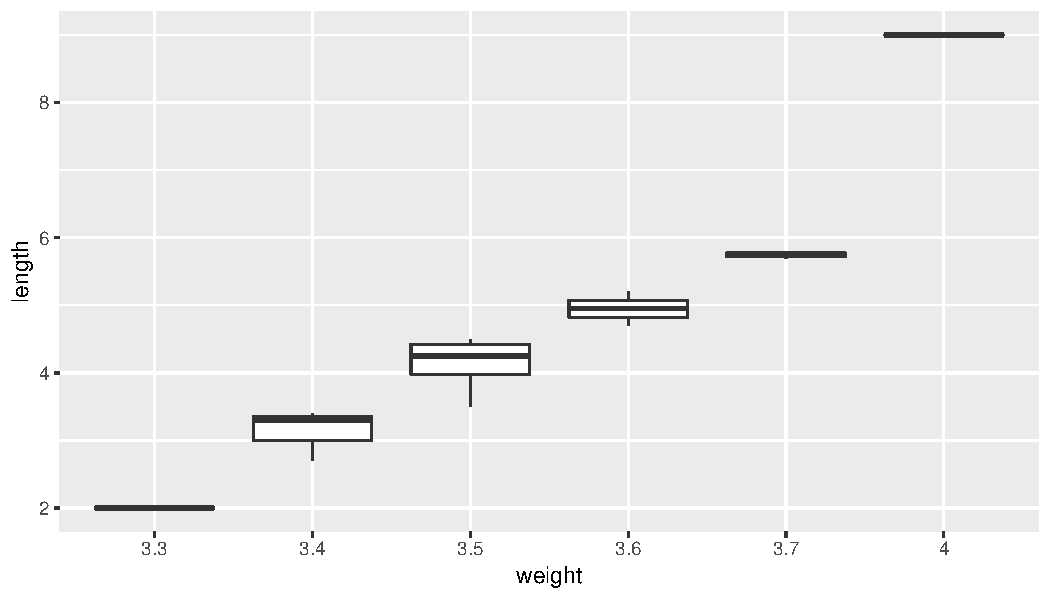
\includegraphics[width=\maxwidth]{figure/crosstable_5-1} 

}

\caption[A box plot of the pencil data]{A box plot of the pencil data.}\label{fig:crosstable_5}
\end{figure}



Suppose we also measure the weight of my pencils in grams. Table \ref{tab:cross-table_4} shows the cross-tabulation of \texttt{length} and \texttt{weight}. This is a very sparse table (i.e., with lots of zeros), which makes it very hard to see any systematic co-variation in \texttt{weight} and \texttt{length}. Figure \ref{fig:crosstable_5} shows a box plot of \texttt{weight} and \texttt{length}. Also this plot seems a bit strange, because for every observed weight value under 4 grams, there is only one observation, so that only the median can be plotted.

Therefore, in cases where we have two numeric variables, we generally use a \textit{scatter plot}. Figure \ref{fig:scatter_1} shows a scatter plot of \texttt{weight} by \texttt{length}. Now, the relationship between \texttt{weight} and \texttt{length} is easily understood: it appears there is a \textit{linear} relationship between \texttt{weight} and \texttt{length}. For every increase in \texttt{weight}, there is also an increase in \texttt{length}. The relationship is called linear because we could summarise the relationship by drawing a straight line through the dots. This line is shown in Figure \ref{fig:line_1}.


\begin{figure}

{\centering 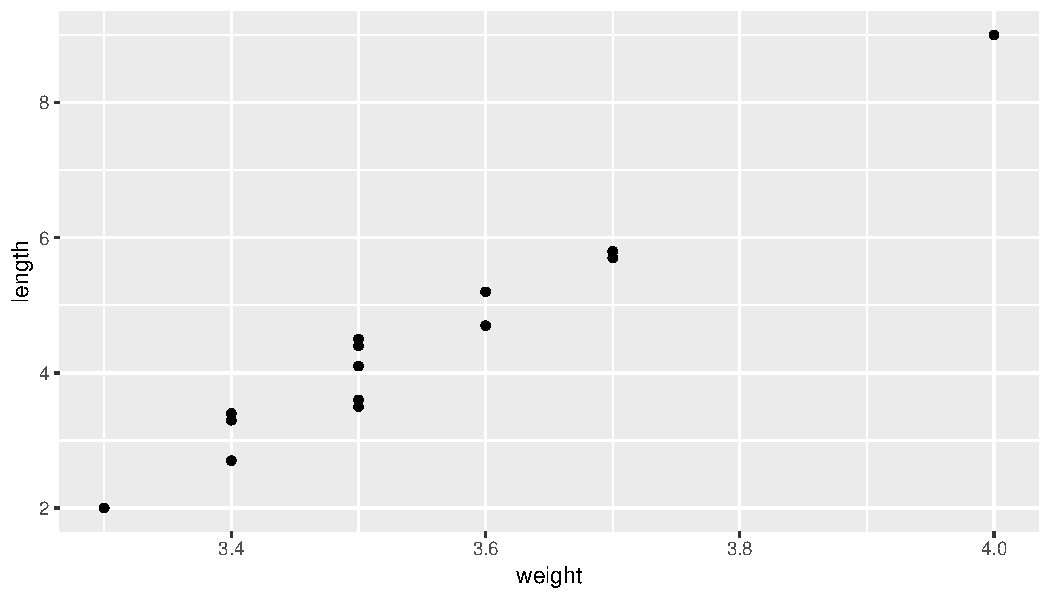
\includegraphics[width=\maxwidth]{figure/scatter_1-1} 

}

\caption[A scatter plot of length and weight]{A scatter plot of length and weight.}\label{fig:scatter_1}
\end{figure}



\begin{figure}

{\centering 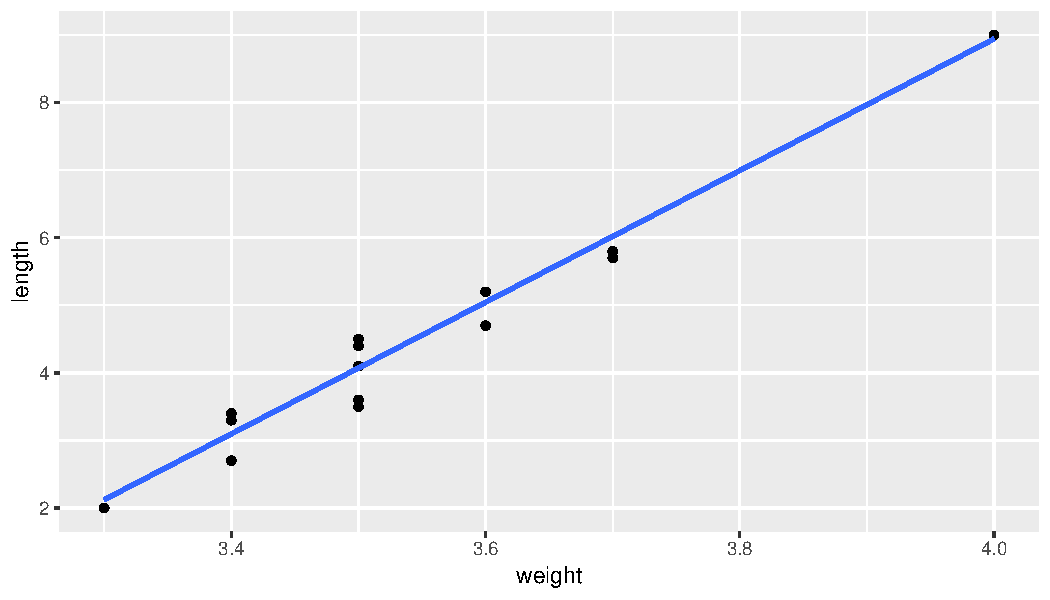
\includegraphics[width=\maxwidth]{figure/line_1-1} 

}

\caption[A scatter plot of length and weight, with a straight line that summarises the relationship]{A scatter plot of length and weight, with a straight line that summarises the relationship.}\label{fig:line_1}
\end{figure}



You see that by visualising two variables, important patterns may emerge that you can easily overlook when only looking at the values. Cross-tables, box plots and scatter plots are powerful tools to find regularities but also oddities in your data that you'd otherwise miss. Some such patterns can be summarised by straight lines, as we see in Figure \ref{fig:line_1}. The remainder of this book focuses on how we can use straight lines to summarise data, but also how to make predictions for data that we have not seen yet.

\section{Visualising two variables using R}

A scatter plot for two numeric variables can be made using \texttt{geom\_point()}:

\begin{knitrout}
\definecolor{shadecolor}{rgb}{0.969, 0.969, 0.969}\color{fgcolor}\begin{kframe}
\begin{alltt}
\hlstd{mtcars} \hlopt
  \hlkwd{ggplot}\hlstd{(}\hlkwd{aes}\hlstd{(}\hlkwc{x} \hlstd{= wt,} \hlkwc{y} \hlstd{= mpg))} \hlopt{+}
  \hlkwd{geom_point}\hlstd{()}
\end{alltt}
\end{kframe}
\end{knitrout}

A box plot for one categorical and one numeric variable can be made using \texttt{geom\_boxplot()}:

\begin{knitrout}
\definecolor{shadecolor}{rgb}{0.969, 0.969, 0.969}\color{fgcolor}\begin{kframe}
\begin{alltt}
\hlstd{mtcars} \hlopt
  \hlkwd{mutate}\hlstd{(}\hlkwc{cyl} \hlstd{=} \hlkwd{factor}\hlstd{(cyl))} \hlopt
  \hlkwd{ggplot}\hlstd{(}\hlkwd{aes}\hlstd{(}\hlkwc{x} \hlstd{= cyl,} \hlkwc{y} \hlstd{= mpg))} \hlopt{+}
  \hlkwd{geom_boxplot}\hlstd{()}
\end{alltt}
\end{kframe}
\end{knitrout}

A cross table for two categorical variables can be made using \texttt{table()}:

\begin{knitrout}
\definecolor{shadecolor}{rgb}{0.969, 0.969, 0.969}\color{fgcolor}\begin{kframe}
\begin{alltt}
\hlkwd{table}\hlstd{(mtcars}\hlopt{$}\hlstd{cyl, mtcars}\hlopt{$}\hlstd{gear)}
\end{alltt}
\begin{verbatim}
##    
##      3  4  5
##   4  1  8  2
##   6  2  4  1
##   8 12  0  2
\end{verbatim}
\end{kframe}
\end{knitrout}

Note that the number of cylinders (first-named variable) is in the rows (here 4, 6 and 8 cylinders), and the number of gears (second-named variable) is in the columns (3, 4, and 5 gears).



\section{Overview of the book}

Chapter \ref{chap:mean} will introduce the problem of \textit{inference}: if you only have a small selection of data points, what can they tell us about the rest of the data? We will use the example of a mean computed using a small number of numerical data points and try to figure out what the mean is likely to be if we would have all the data points. Chapter \ref{chap:prop} discusses the same problem but then for a proportion.

Chapter \ref{chap:simple} will show how we can use a straight line to summarise the relationship between two numeric variables (simple regression), where one variable is the \textit{outcome} variable, and the other variable is a \textit{predictor} variable, that predicts the value on the outcome variable. Such a straight line is a simple form of a \textit{linear model}. We also describe how we can use straight lines (linear models) to summarise relationships between one outcome variable and more than two numeric predictor variables (multiple regression). In Chapter \ref{chap:inf_lm} we will discuss how you can draw conclusions about linear models for data that you have not seen. For example, in the previous section we described the relationship between weight and length of twenty pencils. The question that you may have is whether this linear relationship also holds for \textit{all} pencils of the same make, that is, whether the same linear model holds for both the observed twenty pencils and the total collection of pencils.

In Chapter \ref{chap:categorical} we will show how we can use straight lines to summarise relationships with predictor variables that we want to treat as categorical.

Chapter \ref{chap:assumptions} discusses when it is appropriate to use linear models to summarise your data, and when it is not. It introduces methods that enable you to decide whether to trust a linear model or not. Chapter \ref{chap:nonpar1} then discusses alternative methods that you can use when linear models are not appropriate.

Chapter \ref{chap:moderation} focuses on moderation: how one predictor variable can affect the effect that a second predictor variable has on the outcome variable.

Chapter \ref{chap:advanced} shows how you can make elaborate statements about differences between groups of observations, in case one of the predictor variables is a categorical variable.

Chapters \ref{chap:mixed} and \ref{chap:premidpost} show how to deal with variables that are measured more than once in the same unit of analysis (the same participant, the same pencil, the same school, etc.). For example, you may measure the weight of a pencil before and after you have made a drawing with it. Models that we use for such data are called \textit{linear mixed models}. Similar to linear models, linear mixed models are not always appropriate for some data sets. Therefore, Chapter \ref{chap:nonpar2} discusses alternative methods to study variables that are repeatedly measured in the same research unit.

Chapters \ref{chap:logistic} and \ref{chap:poisson} discuss \textit{generalised linear models}. These are models where the outcome variable is not numeric and continuous. Chapter \ref{chap:logistic} discusses a method that is appropriate when the outcome variable has only two values, say "yes" and "no", or "pass" and "fail". Chapter \ref{chap:poisson} discusses a method that can be used when the outcome variable is a count variable and therefore discrete, for example the number of children in a classroom, or the number of harvested zucchini from one plant.

Chapter \ref{chap:bda} discusses relatively new statistical methodology that is needed when you have a lot of variables. In such cases, traditional inferential data analysis as discussed in the previous chapters often fails. 











 % exploring your data, descriptive statistics label intro



\chapter{Inference about a mean}\label{chap:mean}


% 101.	Sampling distribution of a mean (required unit)
% 
% •	Know difference between population mean and sample mean 
% •	Know what a sampling distribution of the sample mean is. 
% •	Know that you one also can have a sampling distribution of a variance or standard deviation
% •	Central limit theorem: if sample size is large enough, sampling distribution of a single parameter becomes normal, for any type of distribution (except Cauchy).
% 


\begin{knitrout}
\definecolor{shadecolor}{rgb}{0.969, 0.969, 0.969}\color{fgcolor}\begin{figure}
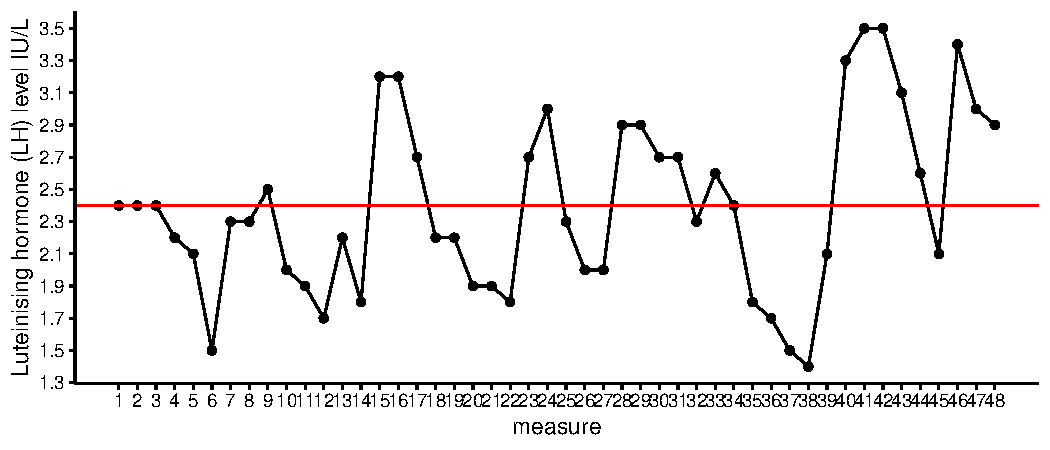
\includegraphics[width=\maxwidth]{figure/mean_data-1} \caption[Luteinising hormone levels measured in one female, 48 measures taken at 10-minute intervals]{Luteinising hormone levels measured in one female, 48 measures taken at 10-minute intervals.}\label{fig:mean_data}
\end{figure}


\end{knitrout}


\section{The problem of inference}

The human body is heavily controlled by hormones. One of the hormones involved in a healthy reproductive system is luteinising hormone (LH). This hormone is present in both females and males, but with different roles. In females, a sudden rise in LH levels triggers ovulation (the release of an egg from an ovary). We have a data set on luteinising hormone (LH) levels in one anonymous female. The data are given in Figure \ref{fig:mean_data}. In this data set, we have 48 measures, taken at 10-minute intervals. We see that LH levels show quite some variation over time. Suppose we want to know the mean level of luteinising hormone level in this woman, how could we do that?

The easiest way is to compute the mean of all the values that we see in this graph. If we do that here, we get the value 2.4. That value is displayed as the red line in Figure \ref{fig:mean_data}. However, is that really the mean of the hormone levels during that time period? The problem is that we only have 48 measures; we do not have information about the hormone levels \textit{in between} measurements. We see some very large differences between two consecutive measures, which makes the level of hormone look quite unstable. We lack information about hormone levels in between measurements because we do not have data on that. We only have information about hormone levels at the times where we have observed data. For the other times, we have unobserved or missing data.

Suppose that instead of the mean of the \textit{observed} hormone levels, we want to know the mean of \textit{all} hormone levels during this time period: not only those that are measured at 10-minute intervals, but also those that are not measured (unobserved/missing). 

You could imagine that if we would measure LH not every 10 minutes, but every 5 minutes, we would have more data, and the mean of those measurements would probably be somewhat different than 2.4. Similarly, if we would take measurements every minute, we again would obtain a different mean. Suppose we want to know what the true mean is: the mean that we would get if we would measure LH continuously, that is, an infinite number of measurements. Unfortunately we only have these 48 measures to go on. We would like to infer from these 48 measures, what the mean is of LH level \textit{had we measured continuously}.


This is the problem of \textit{inference}: how to infer something about complete data, when you only see a small subset of the data. The problem of \textit{statistical inference} is when you want to say something about an imagined complete data set, the \textit{population}, when you only observe a relatively small portion of the data, the \textit{sample}. 

In order to show you how to do that, we do a thought experiment. Imagine a huge data set on African elephants where we measured the height of each elephant currently living (today around 415,000 individuals). Let's imagine that for this huge data set, the mean and the variance are computed: a mean of 3.25 m and a variance of 0.14 (recall, from Chapter \ref{chap:intro}, that the variance is a measure of spread, based on the sums of squared differences between values and the mean). We call this data set of all African elephants currently living the \textit{population} of African elephants. 

Now that we know that the actual mean equals 3.25 and the actual variance equals 0.14, what happens if we only observe 10 of these 415,000 elephants? In our thought experiment we randomly pick 10 elephants. Random means that every living elephant has an equal chance of being picked. This random \textit{sample} of 10 elephants is then used to compute a mean and a variance. Imagine that we do this exercise a lot of times: every time we pick a new random sample of 10 elephants, and you can imagine that each time we get slightly different values for our mean, but also for our variance. This is illustrated in Table \ref{tab:sample_data_01}, where we show the data from 5 different samples (in different columns), together with 5 different means and 5 different variances.

What we see from this table is that the 5 \textit{sample means} vary around the population mean of 3.25, and that the 5 variances vary around the population variance of 0.14. We see that therefore the mean based on only 10 elephants gives a rough approximation of the mean of \textit{all} elephants: the sample mean gives a rough approximation of the population mean. Sometimes it is too low, sometimes it is too high. The same is true for the variance: the variance based on only 10 elephants is a rough approximation, or \textit{estimate}, of the variance of \textit{all} elephants: sometimes it is too low, sometimes it is too high. 


% latex table generated in R 4.0.3 by xtable 1.8-4 package
% Sun Jan 31 16:36:33 2021
\begin{table}[ht]
\centering
\caption{Imaginary data on elephant height when 5 random samples (columns) of 10 elephants (rows) are drawn from the population data.} 
\label{tab:sample_data_01}
\begin{tabular}{rrrrrr}
  \hline
 & 1 & 2 & 3 & 4 & 5 \\ 
  \hline
1 & 3.77 & 2.52 & 3.26 & 3.61 & 3.16 \\ 
  2 & 3.61 & 3.41 & 3.09 & 3.33 & 2.74 \\ 
  3 & 3.12 & 2.91 & 3.14 & 3.22 & 3.91 \\ 
  4 & 2.95 & 3.20 & 2.85 & 3.40 & 3.60 \\ 
  5 & 2.53 & 3.45 & 2.69 & 3.20 & 3.19 \\ 
  6 & 3.12 & 3.11 & 3.45 & 2.31 & 2.94 \\ 
  7 & 3.31 & 3.22 & 2.98 & 3.65 & 4.39 \\ 
  8 & 2.59 & 3.76 & 2.81 & 2.20 & 3.24 \\ 
  9 & 2.91 & 3.44 & 3.63 & 3.12 & 3.21 \\ 
  10 & 3.36 & 2.84 & 4.15 & 2.73 & 2.75 \\ 
  mean & 3.13 & 3.19 & 3.20 & 3.08 & 3.31 \\ 
  variance & 0.14 & 0.12 & 0.18 & 0.23 & 0.24 \\ 
   \hline
\end{tabular}
\end{table}



\section{Sampling distribution of mean and variance}

How high and how low the sample mean can be, is seen in Figure \ref{fig:mean_mean_distribution_N10}. There you see a histogram of all sample means when you draw 10,000 different samples of each consisting of 10 elephants and for each sample compute the mean. This distribution is a \textit{sampling distribution}. More specifically, it is the sampling distribution of the sample mean. 

The red vertical line indicates the mean of the population data, that is, the mean of 3.25 (the population mean). The blue line indicates the mean of all these sample means together (the mean of the sample means). You see that these lines practically overlap.  

What this sampling distribution tells you, is that if you randomly pick 10 elephants from a population, measure their heights, and compute the mean, this mean is \textit{on average} a good estimate (approximation) of the mean height in the population. The mean height in the population is 3.25, and when you look at the sample means in Figure \ref{fig:mean_mean_distribution_N10}, they are generally very close to this value of 3.25. Another thing you may notice from Figure \ref{fig:mean_mean_distribution_N10} is that the sampling distribution of the sample mean looks symmetrical and resembles a normal distribution. 

\begin{knitrout}
\definecolor{shadecolor}{rgb}{0.969, 0.969, 0.969}\color{fgcolor}\begin{figure}
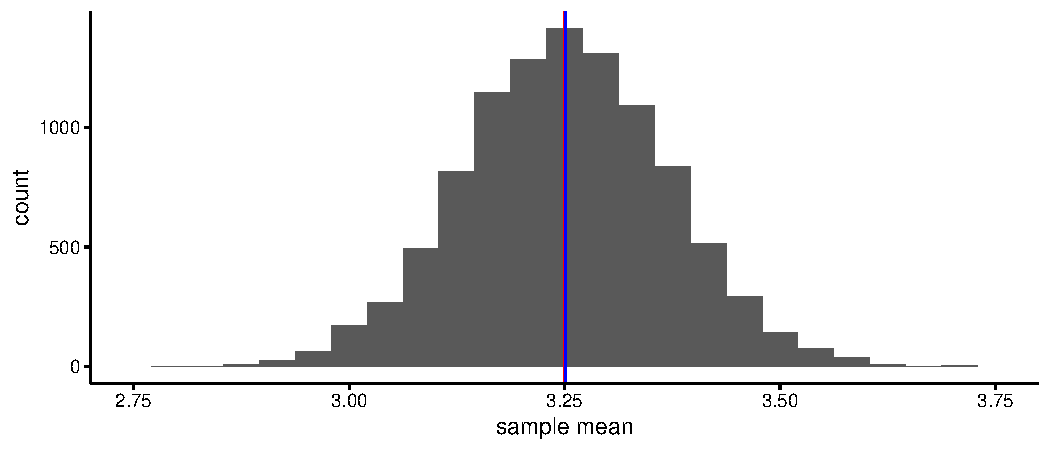
\includegraphics[width=\maxwidth]{figure/mean_mean_distribution_N10-1} \caption[A histogram of 10,000 sample means when the sample size equals 10]{A histogram of 10,000 sample means when the sample size equals 10.}\label{fig:mean_mean_distribution_N10}
\end{figure}


\end{knitrout}

\begin{knitrout}
\definecolor{shadecolor}{rgb}{0.969, 0.969, 0.969}\color{fgcolor}\begin{figure}
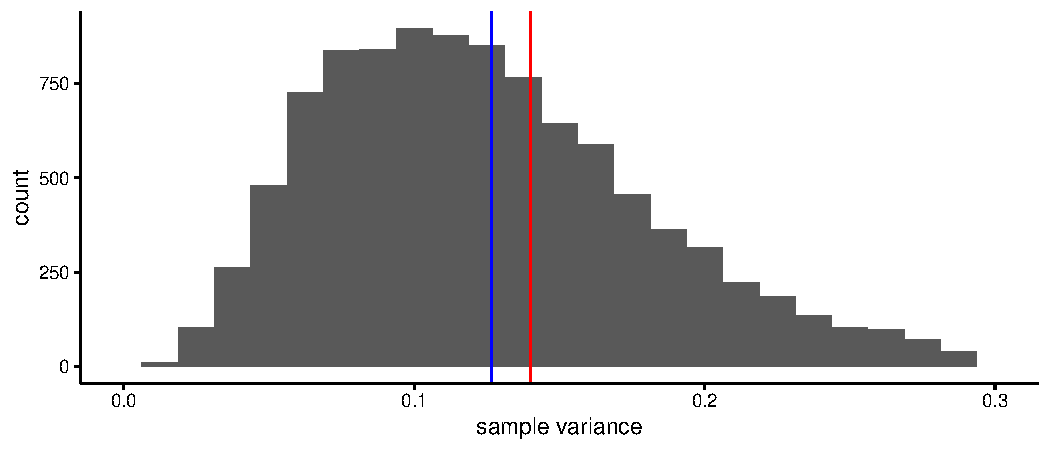
\includegraphics[width=\maxwidth]{figure/mean_var_distribution_N10-1} \caption[A histogram of 10,000 sample variances when the sample size equals 10]{A histogram of 10,000 sample variances when the sample size equals 10. The red line indicates the population variance. The blue line indicates the mean of all variances observed in the 10,000 samples.}\label{fig:mean_var_distribution_N10}
\end{figure}


\end{knitrout}


Now let's look at the sampling distribution of the sample variance. Thus, every time we randomly pick 10 elephants, we not only compute the mean but also the variance. Figure \ref{fig:mean_var_distribution_N10} shows the sampling distribution. The red line shows the variance of the height in the population, and the blue line shows the mean variance observed in the 10,000 samples. Clearly, the red and blue line do not overlap: the mean variance in the samples is slightly lower than the actual variance in the population. We say that the sample variance underestimates the population variance a bit. Sometimes we get a sample variance that is lower than the population value, sometimes we get a value that is higher than the population value, but on average we are on the low side. 


\bigskip



\noindent\fbox{%
    \parbox{\textwidth}{%
\textbf{Overview}
\begin{itemize}

\item \textbf{population}: all values, both observed and unobserved 

\item \textbf{population mean}: the mean of all values (observed and unobserved values)

\item \textbf{sample}: a limited number of observed values

\item \textbf{sample size}: the number of observed values

\item \textbf{sample mean}: the mean of the values in the sample

\item \textbf{random sample}: values that you observe when you randomly pick a subset of the population

\item \textbf{random}: each value in the population has an equal probability of being observed

\item \textbf{sampling distribution of the sample mean}: the distribution of means that you get when you randomly pick new samples from a population and for each sample compute the mean

\item \textbf{sampling distribution of the sample variance}: the distribution of variances that you get when you randomly pick new samples from a population and for each sample compute the variance

\end{itemize}

}%
}


\bigskip






\section{The effect of sample size}\label{sec:sample_size}

What we have seen so far is that when the population mean is 3.25 m and we observe only 10 elephants, we may get a value for the sample mean of somewhere around 3.25, but on average, we're safe to say that the sample mean is a good approximation for the population mean. In statistics, we call the sample mean an \textit{unbiased estimator} of the population mean, as the expected value (the average value we get when we take a lot of samples) is equal to the population value. 

Unfortunately the same could not be said for the variance: the sample variance is not an unbiased estimator for the population variance. We saw that on average, the values for the variances are too low. 

Another thing we saw was that the distribution of the sample means looked symmetrical and close to normal. If we look at the sampling distribution of the sample variance, this was less symmetrical, see Figure \ref{fig:mean_var_distribution_N10}. It actually has the shape of a so-called $\chi^2$-(pronounced 'chi-square') distribution, which will be discussed in Chapters \ref{chap:nonpar1}, \ref{chap:nonpar2}, \ref{chap:logistic} and \ref{chap:poisson}. Let's see what happens when we do not take samples with 10 elephants each time, but 100 elephants. 
\\
\\
Stop and think: What will happen to the sampling distributions of the mean and the variance? For instance, in what way will Figure \ref{fig:mean_mean_distribution_N10} change when we use 100 elephants instead of 10?
\\
\\
Figure \ref{fig:mean_mean_distribution_N100} shows the sampling distribution of the sample mean. Again the distribution looks normal, again the blue and red lines overlap. The only difference with Figure \ref{fig:mean_mean_distribution_N10} is the spread of the distribution: the values of the sample means are now much closer to the population value of 3.25 than with a sample size of 10. That means that if you use 100 elephants instead of 10 elephants to estimate the population mean, on average you get much closer to the true value!
\\
\\
Now stop for a moment and think: is it logical that the sample means are much closer to the population mean when you have 100 instead of 10 elephants?
\\
\\
Yes, of course it is, with 100 elephants you have much more information about elephant heights than with 10 elephants. And if you have more information, you can make a better approximation (estimation) of the population mean.

Figure \ref{fig:mean_var_distribution_N100} shows the sampling distribution of the sample variance. Compared to a sample size of 10, the shape of the distribution now looks more symmetrical and closer to normal. Second, similar to the distribution of the means, there is much less variation in values: all values are now closer to the true value of 0.14. And not only that: it also seems that the bias is less, in that the blue and the red lines are closer to each other. 

Here we see three phenomena. The first is that if you have a statistic like a mean or a variance and you compute that statistic on the basis of randomly picked sample data, the distribution of that statistic (i.e., the sampling distribution) will generally look like a normal distribution if sample size is large enough. 

% heftige nootnoot
It can actually be proven that the distribution of the mean will become a normal distribution if sample size becomes large enough. This phenomenon is known as the Central Limit Theorem. It is true for any population, no matter what distribution it has.\footnote{This is true except for the case that you have fewer than 3 data points and for a few special cases, that you don't need to know about in this book.} Thus, this means that height in elephants itself does not have to be normally distributed, but the sampling distribution of the sample mean will be normal for large sample sizes (e.g., 100 elephants).

The second phenomenon is that the sample mean is an unbiased estimator of the population mean, but that the variance of the sample data is not an unbiased estimator of the population variance. Let's denote the variance of the sample data as $S^2$. Remember from Chapter \ref{chap:intro} that the formula for the variance is


\begin{eqnarray}
S^2 = \mathrm{Var}(Y) = \frac{\Sigma (y_i - \bar{y})^2}{n}
\end{eqnarray}

We saw that the bias was large for small sample size and small for larger sample size. So somehow we need to correct for sample size. It turns out that the correction is a multiplication with $\frac{n}{n-1}$:

\begin{eqnarray}
s^2 = \frac{n}{n-1}{S^2}
\end{eqnarray}

where $s^2$ is the corrected estimator of population variance, $S^2$ is the variance observed in the sample, and $n$ is sample size. When we rewrite this formula and cancel out $n$, we get a more direct way to compute $s^2$: 

\begin{eqnarray}
s^2 = \frac{\Sigma (y_i - \bar{y})^2}{n-1}
\end{eqnarray}

Thus, if we are interested to know the variance or the standard deviation in the population, and we only have sample data, it is better to take the sums of squares and divide by $n-1$, and not by $n$. 


% Box maken verschil variantie steekproef en variantieschatter
% variance of the samplling distribution
% distribution of the variance
% misschien beter apart, variantie 




\begin{eqnarray}
\widehat{\sigma^2} = s^2 = \frac{\Sigma (y_i - \bar{y})^2}{n-1}
\end{eqnarray}

where $\widehat{\sigma^2}$ (pronounced 'sigma-squared hat') signifies the estimator of the population variance (the little hat stands for estimator or estimated value). 

The third phenomenon is that if sample size increases, the variability of the sample statistic gets smaller and smaller: the values of the sample means and the sample variances get closer to their respective population values. We will delve deeper into this phenomenon in the next section. 



\begin{knitrout}
\definecolor{shadecolor}{rgb}{0.969, 0.969, 0.969}\color{fgcolor}\begin{figure}
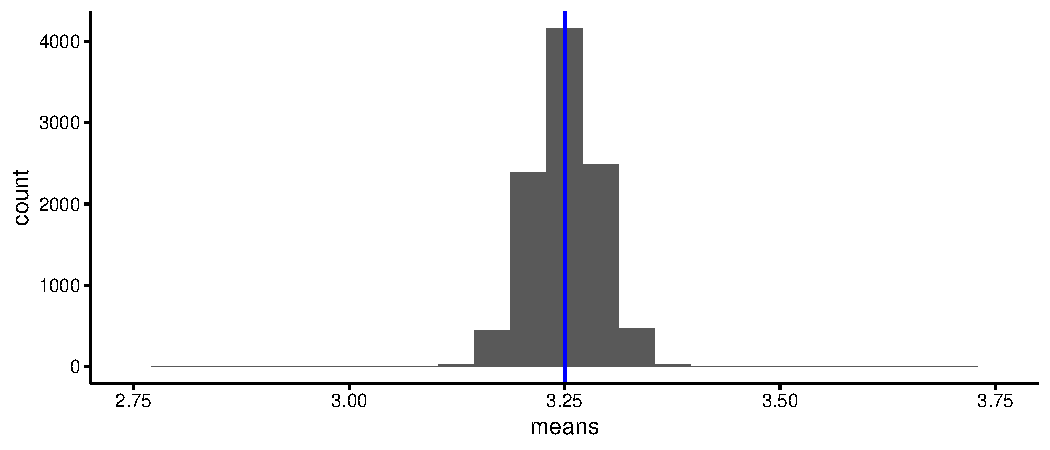
\includegraphics[width=\maxwidth]{figure/mean_mean_distribution_N100-1} \caption[A histogram of 10,000 sample means when the sample size equals 100]{A histogram of 10,000 sample means when the sample size equals 100.}\label{fig:mean_mean_distribution_N100}
\end{figure}


\end{knitrout}

\begin{knitrout}
\definecolor{shadecolor}{rgb}{0.969, 0.969, 0.969}\color{fgcolor}\begin{figure}
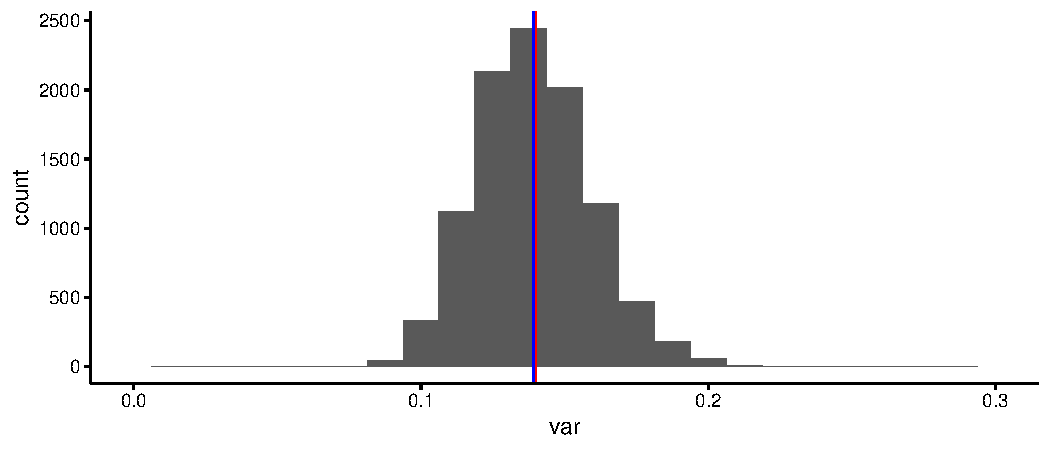
\includegraphics[width=\maxwidth]{figure/mean_var_distribution_N100-1} \caption[A histogram of 10,000 sample variances when the sample size equals 100]{A histogram of 10,000 sample variances when the sample size equals 100.}\label{fig:mean_var_distribution_N100}
\end{figure}


\end{knitrout}


\bigskip



\noindent\fbox{%
    \parbox{\textwidth}{%
\textbf{Overview}
\begin{itemize}

\item \textbf{Central Limit Theorem}: says that the sampling distribution of the sample mean will be normally distributed for infinitely large sample sizes. 

\item \textbf{estimator}: a quantity that you compute based on sample data, that you hope says something about a quantity in the population data. For instance, you can use the sample mean and hope that it is close to the population mean. You use the sample mean as an approximation of the population mean.

\item \textbf{estimate}: the actual value that you get when computing an estimator. For instance, we can use the sample mean as the estimator of the population mean. The formula for the sample mean is $\frac{\Sigma y_i}{n}$ so this formula is our estimator. Based on a sample of 10 values, you might get a sample mean of 3.5. Then 3.5 is the estimate for the population mean.


\item \textbf{unbiased estimator}: an estimator that has the population value as expected value (the mean that you get when averaging over many samples). For example, the sample mean is an unbiased estimator for the population mean because if you draw an infinite number of samples, the mean of the sample means will be equal to the population mean.

\item \textbf{biased estimator}: an estimator that does not have the population value as expected value. For example, the variance calculated using a sample is a biased estimator for the population variance because if you draw an infinite number of samples, the mean of the variances will not be equal to the population variance.


\item $S^2$: the variance of the values in the sample, computed by taking the sum of squares and divide by sample size $n$.

\item $s^2$: an unbiased estimator for the population variance, often confusingly called the 'sample variance', computed by taking the sum of squares and divide by $n-1$.


\end{itemize}

}%
}


\bigskip



% 102.	Standard error and t-distribution (required unit)
% 
% •	Know what a standard error is, what it represents, and how to compute it, given the formula based on the sample data.
% •	Know that if you compute the ratio estimated.mean/standard error, its sampling distribution is not normal but a t-distribution. 
% •	Know what is meant by degrees of freedom in the context of a sample mean and a sample sd.
% 





\section{The standard error}

In Chapter \ref{chap:intro} we saw that a measure for spread and variability was the variance. In the previous section we saw that with sample size 100, the variability of the sample mean was much lower than with sample size 10. Let's look at this more closely. 

When we look at the sampling distribution in Figure \ref{fig:mean_mean_distribution_N10} with sample size 10, we see that the means lie between 2.8 and 3.71. If we compute the standard deviation of the sample means, we obtain a value of 0.118. This standard deviation of the sample means is technically called the \textit{standard error}, in this case the \textit{standard error of the mean}. It is a measure of how uncertain we are about a population mean when we only have sample data to go on. 
\
\
Think about this: why would we associate a large standard error with very little certainty?
\
\
In this case we have only 10 data points for each sample, and it turns out that the standard error of the mean is a function of both the sample size $n$ and the population variance $\sigma^2$. 

\begin{equation}
\sigma_{\bar{y}} =  \sqrt{\frac{\sigma^2}{n}}  
\end{equation}

Here, the population variance equals 0.14 and sample size equals 10, so the $\sigma_{\bar{y}}$ equals $\sqrt{\frac{0.14}{10}} = 0.118$, close to our observed value. If we fill in the formula for a sample size of 100, we obtain a value of 0.037. This is a much smaller value for the spread and this is indeed observed in Figure \ref{fig:mean_mean_distribution_N100}. Figure \ref{fig:se_sample_size} shows the standard error of the mean for all sample sizes between 1 and 200. 

In sum, the standard error of the mean is the standard deviation of the sample means, and serves as a measure of the uncertainty about the population mean. The larger the sample size, the smaller the standard error, the closer a sample mean is expected to be around the population mean, the more certain we can be about the population mean. 

Similar to the standard error of the mean, we can compute the standard error of the variance. This is more complicated -- especially if the population distribution is not normal -- and we do not treat it here. Software can do the computations for you, and later in this book you will see examples of the standard error of the variance.

Summarising the above: when we have a population mean, we usually see that the sample mean is close to it, especially for large sample sizes. If you do not understand this yet, go back before you continue reading.


The larger the sample size, the closer the sample means are to the population means. If you turn this around, if you don't know the population mean, you can use a large sample size, calculate the sample mean, and then you have a fairly good estimate for the population. This is useful for our problem of the LH levels, where we have 48 measures. The mean of the 48 measurements could be a good approximation of the mean LH level in general.

As an indication of how close you are to the population mean, the standard error can be used. The standard error of the mean is the standard deviation of the sampling distribution of the sample mean. The smaller the standard error, the more confident you can be that your sample mean is close to the population mean. In the next section, we look at this more closely. If we use our sample mean as our best guess for the population mean, what would be a sensible range of other possible values for the population mean, given the standard error?


\begin{knitrout}
\definecolor{shadecolor}{rgb}{0.969, 0.969, 0.969}\color{fgcolor}\begin{figure}
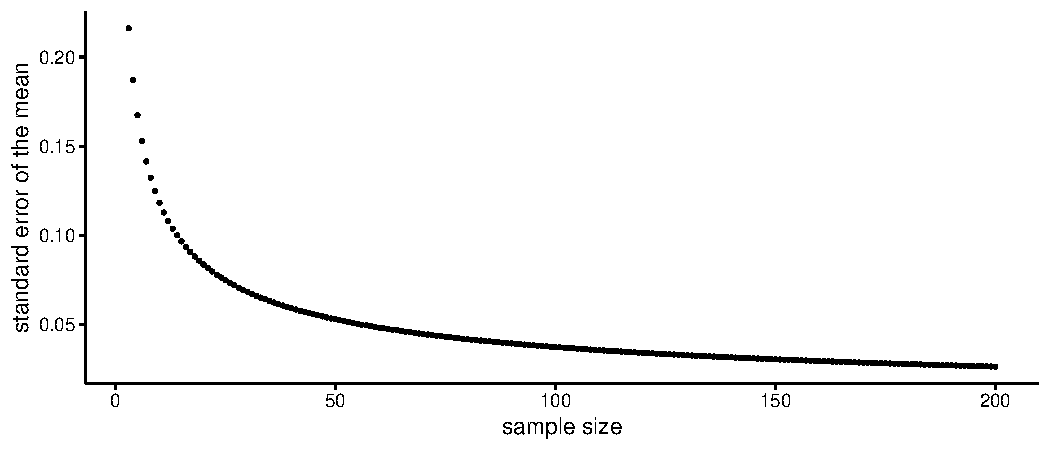
\includegraphics[width=\maxwidth]{figure/se_sample_size-1} \caption[Relationship between sample size and the standard error of the mean, when the population variance equals 0.14]{Relationship between sample size and the standard error of the mean, when the population variance equals 0.14.}\label{fig:se_sample_size}
\end{figure}


\end{knitrout}


\bigskip



\noindent\fbox{%
    \parbox{\textwidth}{%
\textbf{Overview}
\begin{itemize}

\item \textbf{standard error of the mean}: the standard deviation of the distribution of sample means (the sampling distribution of the sample mean). Says something about how spread out the values of the sample means are. It can be used to quantify the uncertainty about the population mean when we only have the sample mean to go on.

\item \textbf{standard error of the variance}: the standard deviation of the sampling distribution of the sample variance. Says something about how spread out the values of the sample variances are. It can be used to quantify the uncertainty about the population variance when we only have the variance of the sample values to go on.


\end{itemize}

}%
}


\bigskip



% 103.	Confidence intervals
% 	
% •	Given sample mean and sample variance, can compute 95\% confidence intervals for the population mean, (by looking up various 
% •	Databegrip,
% •	Reasonable values.
% •	Breed small, welke punten zittern er wel niet in, positief negatief,
% •	critical t-values in a table). 
% •	Can interpret a confidence interval.
% 
% 



\section{Confidence intervals}

% lastig, veel dingen tegelijk.

If we take a sample mean as our best guess of the population mean, we know that we are probably a little bit off. If we have a large standard error we know that the population mean could be very different from our best guess, and if we have a small standard error we know that the true population mean is pretty close to our best guess, but could we quantify this in a better way? Could we give a range of plausible values for the population mean?

In order to do that, let's go back to the elephants: the true population mean is 3.25 m with variance 0.14. What would possible values of sample means look like if sample size is 4? Of course it would look like the sampling distribution of the sample mean with a sample size of 4. Its mean would be the population mean of 3.25 and its standard deviation would be equivalent to the standard error, computed as a function of the population variance and sample size, in our case $\sqrt{\frac{0.14}{4}}= 0.19$. Now imagine that for a bunch of samples we compute the sample means. We know that the means for large sample sizes will look more or less like a normal distribution, but how about for a small sample size like $n=4$? If it would look like a normal distribution too, then we could use the knowledge about the standard normal distribution to say something about the distribution of the sample means. 


For the moment, let's assume the sample size is not 4, but 4000. From the Central Limit Theorem we know that the distribution of sample means is almost identical to a normal distribution, so let's assume it is normal. From the normal distribution, we know that 68\% of the observations lies between 1 \textit{standard deviation} below and 1 \textit{standard deviation} above the mean (see Section \ref{sec:normal} and Figure \ref{fig:distr_4}). If we would therefore standardise our sample means, we could say something about their distribution given the standard error, since the standard error is the standard deviation of the sampling distribution. Thus, if the sampling distribution looks normal, then we know that 68\% of the sample means lies between one \textit{standard error} below the population mean and one \textit{standard error} above the population mean. 

So suppose we take a large number of samples from the population, compute means and variances for each sample, so that we can compute standardised scores. Remember from Chapter \ref{chap:intro} that a standardised score is obtained by subtracting an observed score from the mean and divide by the standard deviation:

\begin{equation}
z_y = \frac{y - \bar{y}}{sd_y}
\end{equation}

If we apply standardisation of the sample means, we get the following: for a given sample mean $\bar{y}$ we subtract the population mean $\mu$ and divide by the standard deviation of the sample means (the standard error):


\begin{equation}
z_{\bar{y}} = \frac{\bar{y} - \mu}{\sigma_{\bar{y}}}
\end{equation}


If we then have a bunch of standardised sample means, their distribution should have a standard normal distribution with mean 0 and variance 1. We know that for this standard normal distribution, 68\% of the values lie between -1 and +1, meaning that 68\% of the values in a non-standardised situation lie between -1 and +1 standard deviations from the mean (see Section \ref{sec:normal}). That implies that 68\% of the sample means lie between -1 and +1 standard deviations (standard errors!) from the population mean. Thus, 68\% of the sample means lie between $-1 \times \sigma_{\bar{y}}$ and $+1 \times \sigma_{\bar{y}}$ from the population mean $\mu$. If we have sample size 4000, $\sigma_{\bar{y}}$ is equal to $\sqrt{\frac{0.14}{4000}} = 0.0059161$ and $\mu = 3.25$, so that 68\% of the sample means lie between 3.2440839 and 3.2559161.

This means that we also know that $100-68=32$\% of the sample means lie farther away from the mean: that it occurs in only 32\% of the samples that a sample mean is smaller than 3.2440839 and larger than 3.2559161. Taking this a bit further, since we know that 95\% of the values in a standard normal distribution lie between -1.96 and +1.96 (see Section \ref{sec:normal}), we know that it happens in only 5\% of the samples that the sample mean is smaller than $3.25 - 1.96 \times \sqrt{\frac{0.14}{4000}} = 3.2384045$ or larger than $3.25 + 1.96 \times \sqrt{\frac{0.14}{4000}} = 3.2615955$. Another way of putting this is that it happens in only 95\% of the samples that a sample mean is at most $1.96 \times \sqrt{\frac{0.14}{4000}}$ away from the population mean 3.25. This distance of 1.96 times the standard error is called the \textit{margin of error} (MoE). Here we focus on the margin of error that is based on 95\% observations of the observations seen in the normal distribution:

\begin{equation}
MoE_{0.95} = z_{0.95} \times \sigma_{\bar{y}} = 1.96 \times \sigma_{\bar{y}}
\end{equation}

where $z_{0.95}$ is the standardised value $z$ for which holds that 95\% of the values are between $\mu- z$ and $\mu+ z$ (i.e., 1.96). 

Knowing the population mean, we know that it is very improbable (5\%) that a sample mean is farther away from the population mean than this margin of error. The next step is tricky, so pay close attention. If we know the population mean, we can construct an interval based on the margin of error for where we expect sample means to lie. In the above case, knowing that the population mean is 3.25, and we use an MoE based on 95\%, we expect that 95\% of the sample means will lie between $3.25 - \textrm{MoE}$ and $3.25 + \textrm{MoE}$. 

But what if we don't know the population mean, but do know the sample mean? We could use the same interval but centred around the sample mean instead of the population mean. Thus, we have a 95\% interval if we take the sample mean as the centre and the MoE around it. Suppose that we randomly draw 4000 elephants and we obtain a sample mean of $\bar{y} = 3.26$, then we construct the 95\% interval as running from $\bar{y} - MoE = 3.26 - MoE$ to $\bar{y} + MoE = 3.26 + MoE$. The margin of error is based on the standard error, which is in turn dependent on the population variance. If we don't know that, we have to estimate it from the sample. So suppose we find a sample variance $s^2 = 0.15$, we get the 95\% interval from $\bar{y} - MoE = 3.26 - 1.96 \times \sqrt{\frac{0.15}{4000}}$ to $\bar{y} + MoE = 3.26 + 1.96 \times \sqrt{\frac{0.15}{4000}}$.

Such an interval, centred around the \textit{sample} mean, is called a \textit{confidence interval}. Because it is based on 95\% of the sampling distribution (centred around the \textit{population} mean) it is called a 95\% confidence interval. 

One way of thinking about this interval is that it represents 95\% of the sample means \textit{had the population mean been equal to the sample mean}. For example, a 95\% interval around the sample mean of 3.26 represents 95\% of the sample means that you would get if you would take many random samples from a population distribution with mean 3.26: the middle 95\% of the sampling distribution for a population mean of 3.26.

\bigskip


\noindent\fbox{%
    \parbox{\textwidth}{%
A 95\% confidence interval contains 95\% of the sample means \textit{had  the  population  mean  been  equal  to  the  sample  mean}. Its construction is based on the estimated sampling distribution of the sample mean.

}%
}


\bigskip


The idea is illustrated in Figure \ref{fig:confidence_interval_explained}. There you see two sampling distributions: one for if the population mean is 3.25 (blue) and one for if the population mean is 3.26 (black). Both are normal distributions because sample size is large, and both have the same standard error that can be estimated using the sample variance. Whatever the true population mean, we can estimate the margin of error that goes with 95\% of the sampling distribution. We can then construct an interval that stretches the length of about twice (i.e., 1.96) the margin of error around any value. We can do that for the real population mean (in blue), but the problem that we face in practice is that we don't know the population mean. We do know the sample mean, and if we centre the interval around that value, we get what is called the 95\% confidence interval. We see that it ranges from 3.248 to 3.272. This we can use as a range of plausible values for the unknown population mean. With some level of 'confidence' we can say that the population mean is somewhere in this interval.

Note that when we say: the 95\% confidence interval runs from 3.248 to 3.272, we cannot say, we are 95\% sure that the population mean is in there. 'Confidence' is not the same as probability. We'll talk about this in a later section. First, we look at the situation where sample size is small so that we cannot use the Central Limit Theorem.






\begin{knitrout}
\definecolor{shadecolor}{rgb}{0.969, 0.969, 0.969}\color{fgcolor}\begin{figure}
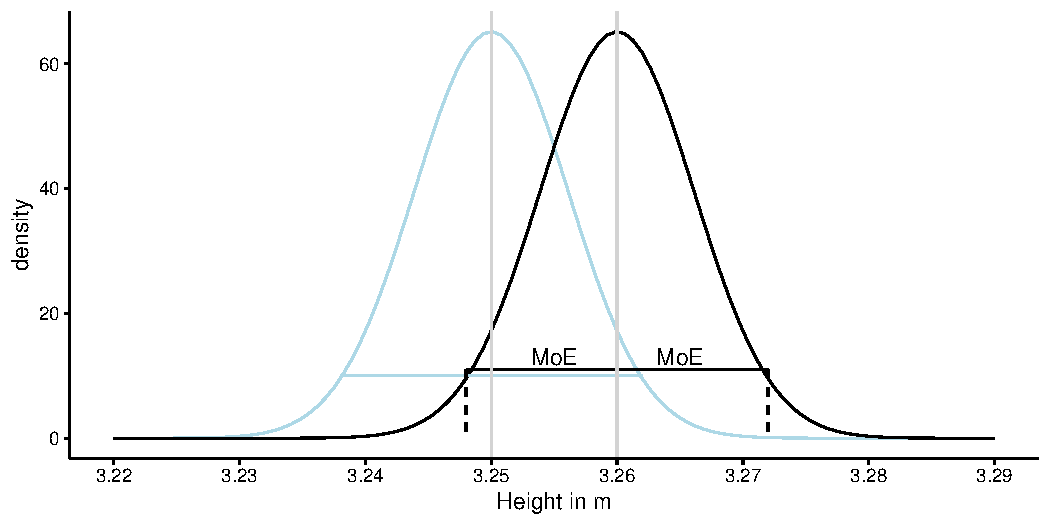
\includegraphics[width=\maxwidth]{figure/confidence_interval_explained-1} \caption{Illustration of the construction of a 95{\%} confidence interval. Suppose we find a sample mean of 3.26 and a sample variance of 0.15, with $n = 4000$. The black curve represents the sampling distribution if the population mean would be 3.26 and a variance of 0.15. In reality, we don't know the population mean, it could be 3.25 or any other value. The sampling distribution for 3.25 is shown by the blue curve. Whatever the case, the length of an interval that contains 95{\%} of the sample means is always the same: twice the margin of error. This interval centred around the sample mean, is called the 95{\%} confidence interval.}\label{fig:confidence_interval_explained}
\end{figure}


\end{knitrout}


\section{The $t$-statistic}


In the previous section, we constructed a 95\% confidence interval based on the standard normal distribution. We know from the standard normal distribution that 95\% of the values are between -1.96 and +1.96. We used the standard normal distribution because the sampling distribution will look normal if sample size is large. We took the example of a sample size of 4000, and then this approach works fine, but remember that the actual sample size was 4. What if sample size is not large? Let's see what the sampling distribution looks like in that case.

Remember from the previous section that we standardised the sample means.

$$z_{\bar{y}} =  \frac{\bar{y}- \mu}{\sigma_{\bar{y}}}$$

and that $z_{\bar{y}}$ has a standard normal distribution. But, this only works if we have a good estimate of $\sigma_{\bar{y}}$, the standard error. If sample size is limited, our estimate is not perfect. You can probably imagine that if you take one sample of 4 randomly selected elephants, you get one value for the estimated standard error ($\sqrt{\frac{s^2}{n}}$), and if you take another sample of 4 elephants, you get a slightly different value for the estimated standard error. Because we do not always have a good estimate for $\sigma_{\bar{y}}$, the standardisation becomes a bit more tricky. Let's call the standardised sample mean $t$ instead of $z$:

$$ t_{\bar{y}_i} =  \frac{\bar{y}_i - \mu}{\sqrt{\frac{s^2_i}{n}}}  $$

Thus, a standardised sample mean for sample $i$, will be constructed using an estimate for the standard error by computing the sample variance $s^2$ for sample $i$. 

If you standardise every sample mean, each time using a slighly different standard deviation, and you plot a histogram of the $t$-values, you do not get a standard normal distribution, but a slightly different one.  


In summary: if you know the standard error (because you know the population variance), the standardised sample means will show a normal distribution. If you don't know the standard error, you have to estimate it based on the sample variance. If sample size is really large, you can estimate the population variance pretty well, and the sample variances will be very similar to each other. In that case, the sampling distribution will look very much like a normal distribution. But if sample size is relatively small, each sample will show a different sample variance, resulting in different standard error estimates. If you standardise each sample mean with a different standard error, the sampling distribution will not look normal. This distribution is called a $t$-distribution. The difference between this distribution and the standard normal distribution is shown in Figure \ref{fig:t3}. The blue curve is the standard normal distribution, the red curve is the distribution we get if we have sample size 4 and we compute $ t_{\bar{y}_i} =  \frac{\bar{y}_i - \mu}{\sqrt{\frac{s^2_i}{n}}}  $ for many different samples.



\begin{knitrout}
\definecolor{shadecolor}{rgb}{0.969, 0.969, 0.969}\color{fgcolor}\begin{figure}

{\centering 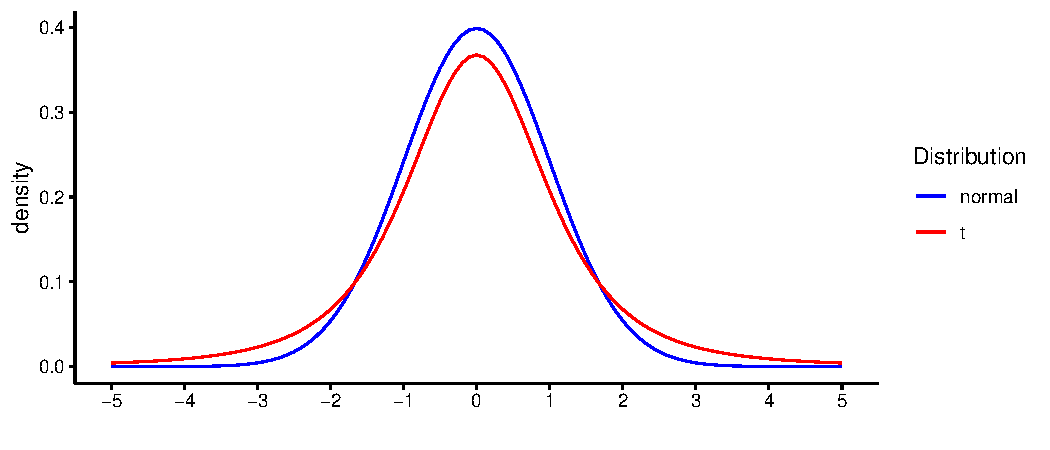
\includegraphics[width=\maxwidth]{figure/t3-1} 

}

\caption[Distribution of \textit{t} with sample size 4, compared with the standard normal distribution]{Distribution of \textit{t} with sample size 4, compared with the standard normal distribution.}\label{fig:t3}
\end{figure}


\end{knitrout}

When you compare the two distributions, you see that compared to the normal curve, there are fewer observations around 0 for the $t$-distribution: the density around 0 is lower for the red curve than for the blue curve. That's because there are more observations far away from 0: in the tails of the distributions, you see a higher density for the red curve ($t$) than for the blue curve (normal). They call this phenomenon 'heavy-tailed': relatively more observations in the tails than around the mean.


That the $t$-distribution is heavy-tailed has important implications. From the standard normal distribution, we know that 5\% of the observations lie more than 1.96 away from the mean. But since there are relatively more observations in the tails of the $t$-distribution, 5\% of the values lie farther away from the mean than 1.96. This is illustrated in Figure \ref{fig:t3_shaded}. If we want to construct a 95\% confidence interval, we can therefore no longer use the 1.96 value. 

\begin{knitrout}
\definecolor{shadecolor}{rgb}{0.969, 0.969, 0.969}\color{fgcolor}\begin{figure}

{\centering 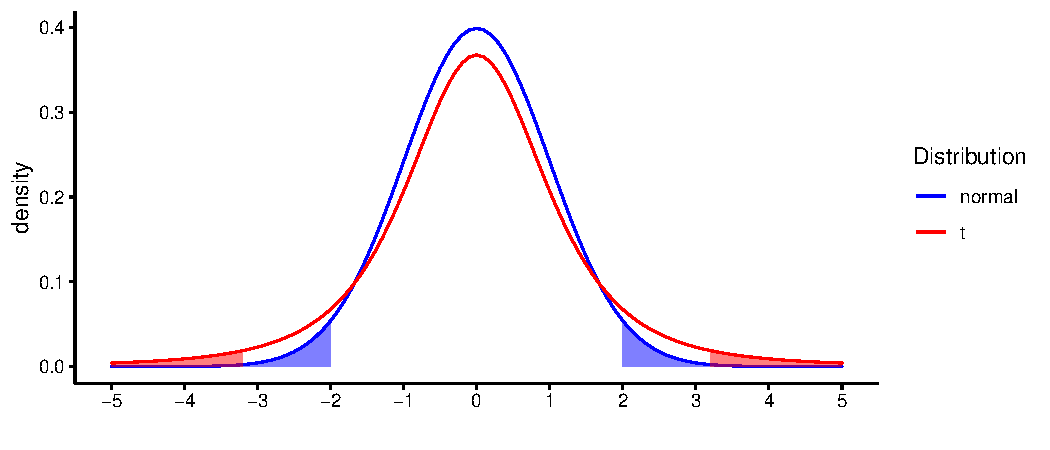
\includegraphics[width=\maxwidth]{figure/t3_shaded-1} 

}

\caption{Distribution of \textit{t} with sample size 4, compared with the standard normal distribution. Shaded areas represent 2.5{\%} of the respective distribution.}\label{fig:t3_shaded}
\end{figure}


\end{knitrout}






With this $t$-distribution, 95\% of the observations lie between -3.18 and +3.18. Of course, that is in the standardised situation. If we move back to our scale of elephant heights with a sample mean of 3.26, we have to transform this back to elephant heights. So -3.18 times the standard error away from the mean of 3.26, is equal to $3.26 - 3.18 \times \sqrt{\frac{0.15}{4}} = 2.6441956$, and +3.18 times the standard error away from the mean of 3.26, is equal to $3.26 + 3.18 \times \sqrt{\frac{0.15}{4}} = 3.8758044$. So the 95\% interval runs from 2.64 to 3.88. This interval is called the 95\% confidence interval, because 95\% of the sample means will lie in this interval, if the population mean would be 3.26.

Notice that the interval includes the population mean of 3.25. If we would interpret this interval around 3.26 as containing plausible values for the population mean, we see that in this case, this is a fair conclusion, because the true value 3.25 lies within this interval.


\section{Interpreting confidence intervals}

The interpretation of confidence intervals is very difficult, and it often goes wrong, even in many textbooks on the matter.

One thing that should be very clear is that a confidence interval is constructed \textit{as if you know the population mean and variance}, which, of course, you don't. We assume that the population mean is a certain value, say $\mu=m_0$, we assume that the standard error of the mean is equal to $\sigma_{\bar{y}}$, and we know that if we would look at many many samples and compute standardised sample means (by using sample means $\bar{y}$ and sample variances $s^2$), their distribution would be a $t$-distribution. Based on that $t$-distribution, we know in which interval 95\% of the standardised sample means would lie and we use that to compute the margin of error and to construct an interval around the sample mean that we actually obtain. A lot of this reasoning is imagination: imagining that you know the population mean and the population variance. Then you imagine what sample means would be reasonable to find and what sample variances. But of course, it's in fact the opposite: you only know the mean and variance of \textit{one} sample and you want to know what are plausible values for the population mean.

You have to bear this reversal in mind when interpreting the 95\% confidence interval around a sample mean. Many people state the following: with 95\% probability, the 95\% confidence interval contains the population mean. This is wrong. It is actually the opposite: the 95\% interval around the population mean contains 95\% of the sample means. 

If you know the population mean $\mu$, then 95\% of the confidence intervals that you construct around the sample means that you get from random sampling will contain the mean $\mu$. This is illustrated in Figure \ref{fig:confints95}. Suppose we take $\mu = 3.25$. Then if we imagine that we take 100 random samples from this population distribution, we can calculate 100 sample means and 100 sample variances. If we then construct 100 confidence intervals around these 100 sample means, we obtain the confidence intervals displayed in Figure \ref{fig:confints95}. We see that 95 of these intervals contain the value 3.25, and 5 of them don't: only in samples 1, 15, 20, 28 and 36, the interval does not contain 3.25.

It can be mathematically shown that given a certain population mean, when taking many, many samples and constructing 95\% confidence intervals, you can expect 95\% of them will contain that population mean. That does \textit{not} mean however that given a sample mean with a certain 95\% interval, that interval contains the population mean with a probability of 95\%. It only means that were this procedure of constructing confidence intervals to be repeated on numerous samples, the fraction of calculated confidence intervals that contain the true population mean would tend toward 95\%. If you only do it once (you obtain a sample mean and you calculate the 95\% confidence interval) it either contains the population mean or it doesn't: you cannot calculate a probability for this. In the statistical framework that we use in this book, one can only say something about the probability of data occurring given some population values: 

\bigskip

\noindent\fbox{%
    \parbox{\textwidth}{%
\textit{Given} that the population value is 3.25, and if you take many, many independent samples from the population, you can expect that 95\% of the confidence intervals constructed based on resulting sample means will contain that population value of 3.25. 

}%
}

\bigskip


% 
% <<>>=
% mu <- c(rep(3.25, 80), rep(3.26, 20))
% value_in_interval <- c(rep("Yes", 0.95 * 80) , rep("No", 0.05 * 80), 
%                        rep("Yes", 0.90 * 20) , rep("No", 0.10 * 20))
% table(value_in_interval, mu) %>% 
%   xtable(caption = "Cross-tabulation of the true population mean (3.25 or 3.26) and whether 3.25 is in the 95{\\%} confidence interval around the sample mean.", 
%          label = "tab:cross-table_95", 
%          digits = 0) %>%
%   print(include.rownames = T, caption.placement = "top")
% 
% @
% 









Using this insight, we therefore conclude that the fact we see the value of 3.25 in our 95\% confidence interval around 2.9, gives us some reason to believe ('confidence') that 3.25 could also be a plausible candidate for the population mean. 

Summarising, if we find a sample mean of say 2.9, we know that 2.9 is a reasonable guess for the population mean (it's an unbiased estimator). Moreover, if we construct a 95\% confidence interval around this sample mean, this interval contains other plausable candidates for the population mean. However, it might be possible that the true population mean is not included.



\begin{knitrout}
\definecolor{shadecolor}{rgb}{0.969, 0.969, 0.969}\color{fgcolor}\begin{figure}

{\centering 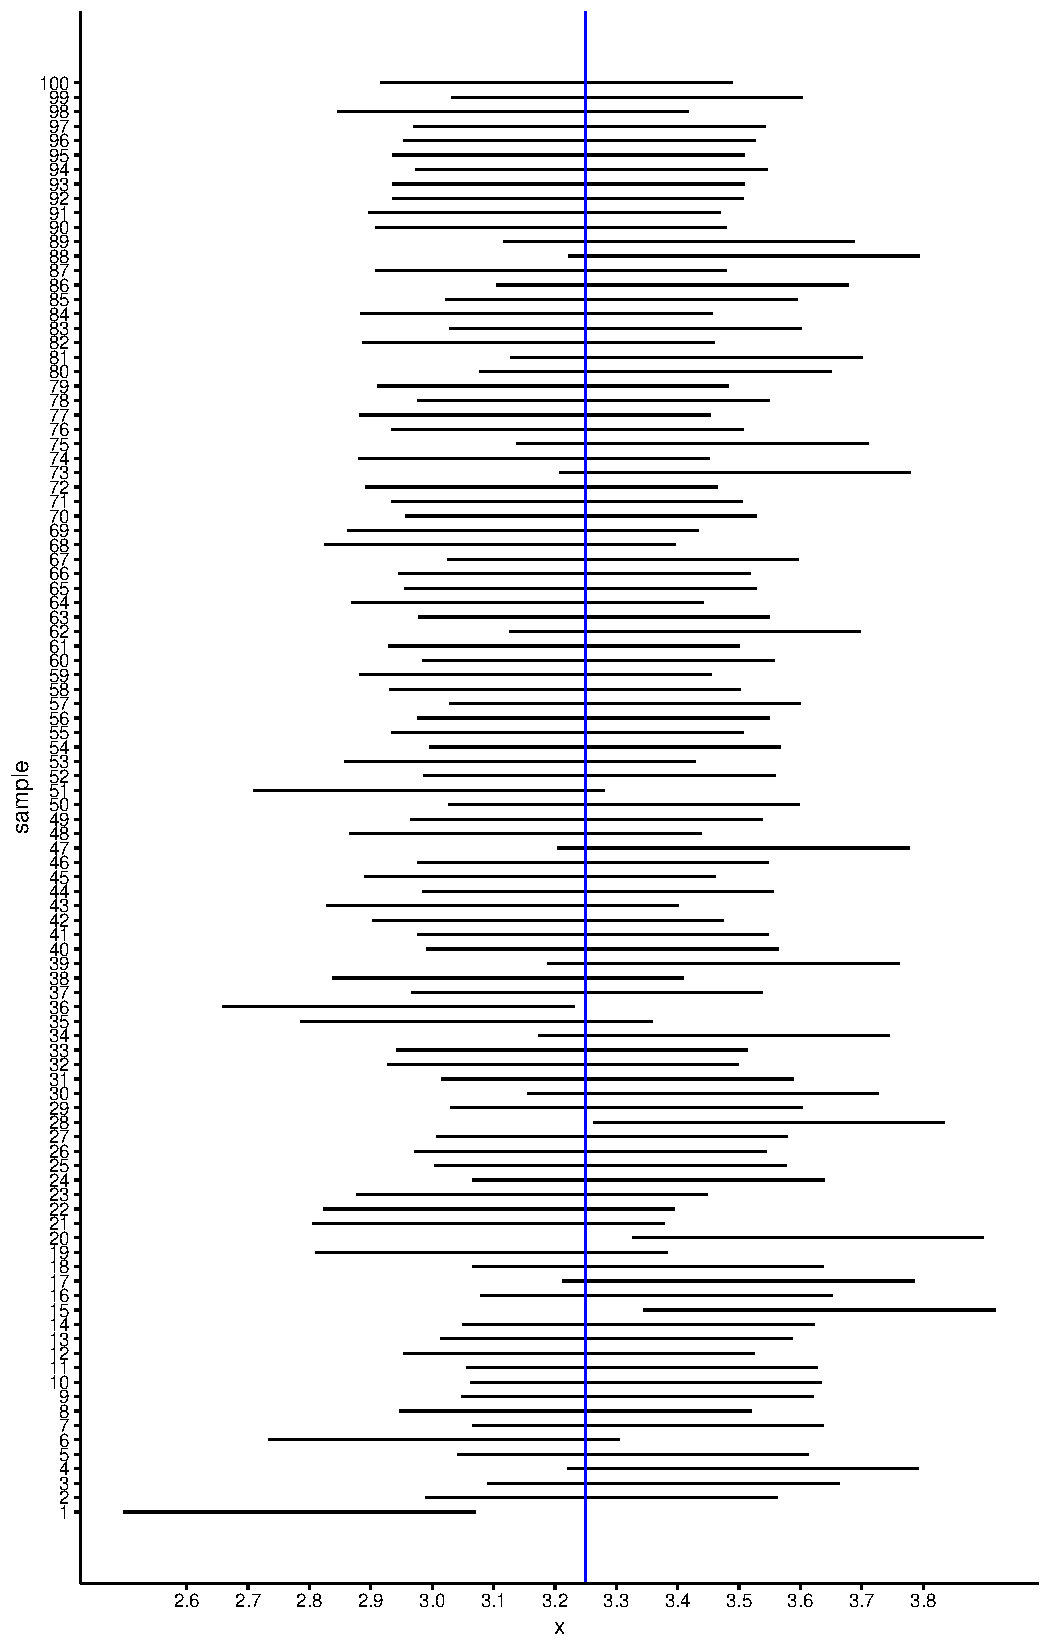
\includegraphics[width=\maxwidth]{figure/confints95-1} 

}

\caption[Confidence intervals]{Confidence intervals.}\label{fig:confints95}
\end{figure}


\end{knitrout}




\section{$t$-distributions and degrees of freedom}

The standardised deviation of a sample mean from a hypothesised population mean has a $t$-distribution. This happens when the population variance is not known, and we therefore have to estimate the standard error based on the sample variance. Because of this uncertainty about the population variance and consequently the standard error, the standardised score does not have a normal distribution but a $t$-distribution.

In the previous section we saw the distribution for the case that we had a sample size of 4. With such a small sample size, we have a very inaccurate estimate of the population variance. The sample variance $s^2$ will be very different for every new sample of size 4. But if sample size increases, our estimates for the population variance will become more precise, and they will show less variability. This results in the sampling distribution to become less heavy-tailed, until it closely resembles the normal distribution for very large sample sizes. 

This means that the shape of the sampling distribution is a $t$-distribution but that the shape of this $t$-distribution depends on sample size. More precisely, the shape of the $t$-distribution depends on its so-called \textit{degrees of freedom} (explained below). Degrees of freedom are directly linked to the sample size. Degrees of freedom can be as small as 1, very large like 250, or infinitely larger. The $t$-distribution with many degrees of freedom like 2500, is practically indistinguishable from a normal distribution. However for a relatively low number of degrees of freedom, the shape is very different: relatively more observations are in the tails of the distribution and less so in the middle, compared to the normal distribution, see Figure \ref{fig:inf_8b}. 



The shape of the $t$-distribution is determined by its degrees of freedom: the higher the degrees of freedom, the more it resembles the normal distribution. So which $t$-distribution do we have to use when we are dealing with sample means and we want to infer something about the population mean, and what are degrees of freedom? As stated already above, the degrees of freedom is directly related to sample size: sample size determines the degrees of freedom of the $t$-distribution that we need. Degrees of freedom stands for the amount of information that we have and of course that depends on how many data values we have. In its most general case, the number of degrees of freedom is the number of values in the final calculation of a statistic that are free to vary. More specifically in our case, the degrees of freedom for a statistic like $t$ are equal to the number of independent scores that go into the estimate, minus the number of parameters used as intermediate steps in the estimation of the parameter itself.


In the example above we had information about 4 elephants (4 values), so our information content is 4. However, remember that when we construct our $t$-value, we have to first compute the sample mean in order to compute the sample variance $s^2$. But, suppose you know the sample mean, you don't have to know all the 4 values anymore. Suppose the heights of the first three elephants are 3.24, 3.25 and 3.26, and someone computes the mean of all four elephants as 3.25, then you automatically know that the fourth elephant has a height of 3.25 (why?). Thus, once you know the mean of $n$ elephants, you can give imaginary values for the heights of only $n-1$ elephants, because given the other heights and the mean, it is already determined. 

The same is true for the $t$-statistic: once you know 3 elephant heights and statistic $t$, then you know the height of the fourth elephant automatically.



Because we assume the mean in our computation of $s^2$ (we fix it) we loose one information point, leaving 3. The shape of the standardised scores of fictitious new samples then looks like a $t$-distribution with 3 degrees of freedom. 

Generally, if we have a sample size of $n$ and the population variance is unknown, the shape of the standardised sample means (i.e., $t$-scores) of fictitious new samples is that of a $t$-distribution with $n-1$ degrees of freedom.





\begin{knitrout}
\definecolor{shadecolor}{rgb}{0.969, 0.969, 0.969}\color{fgcolor}\begin{figure}

{\centering 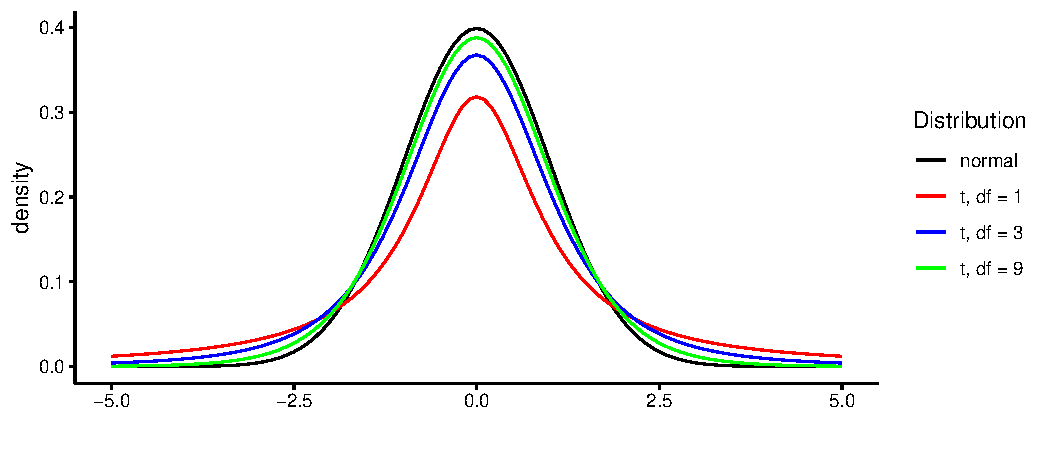
\includegraphics[width=\maxwidth]{figure/inf_8b-1} 

}

\caption[Difference in the shapes of the standard normal distribution and \textit{t}-distributions with 1, 3 and 9 degrees of freedom]{Difference in the shapes of the standard normal distribution and \textit{t}-distributions with 1, 3 and 9 degrees of freedom.}\label{fig:inf_8b}
\end{figure}


\end{knitrout}






\section{Constructing confidence intervals}

In previous sections we discussed the 95\% confidence interval, because it is the most widely used interval. But other intervals are also seen, for instance 99\% confidence intervals or 90\% confidence intervals. A 99\% confidence interval is wider than a 95\% confidence interval, which in turn is wider than a 90\% confidence interval. The width of the confidence interval also depends on the sample size. Here we show how to construct 90\%, 99\% and other intervals, for different sample sizes. 

As we discussed for the 95\% interval above, we looked at the $t$-distribution of 3 degrees of freedom because we had a sample size of 4 elephants. Suppose we have a sample size of 200, then we would have to look at a $t$-distribution of $200-1 = 199$ degrees of freedom. Table \ref{tab:t_table} shows information about a couple of $t$-distributions with different degrees of freedom. In the first column, cumulative probabilities are given, and the next column gives the respective quantiles. For instance, the column 'norm' shows that a cumulative proportion of 0.025 is associated with a quantile of -1.96 for the standard normal distribution. This means that for the normal distribution, 2.5\% of the observations are smaller than -1.96. In the same column we see that the quantile 1.96 is associated with a cumulative probability of 0.975. This means that 97.5\% of the observations in a normal distribution are smaller than 1.96. This implies that 100\% - 97.5\% = 2.5\% of the observations are larger than 1.96. Thus, if 2.5\% of the observations are larger than 1.96 and 2.5\% of the observations are smaller than -1.96, then 5\% of the observations are outside the interval (-1.96, 1.96), and 95\% are inside this interval.

From Table \ref{tab:t_table}, we see that for such a 95\% interval, we have to use the values -1.96 and 1.96 for the normal distribution, but for the $t$-distribution we have to use other values, depending on the degrees of freedom. We see that for 3 degrees of freedom, we have to use the values -3.18 and 3.18, and for 199 degrees of freedom the values -1.97 and +1.97. This means that for a $t$-distribution with 3 degrees of freedom, 95\% of the observations lie in the interval from -3.18 to 3.18. Similarly, for a $t$-distribution with 199 degrees of freedom, the values for cumulative probabilities 0.025 and 0.975 are -1.97 and 1.97 respectively, so we can conclude that 95\% of the observations lie in the interval from -1.97 to 1.97. 

Now instead of looking at 95\% intervals for the $t$-distribution, let's try to construct a 90\% confidence interval around an observed sample mean. With a 90\% confidence interval, 10\% lies outside the interval. We can divide that equally to 5\% on the low side and 5\% on the high side. We therefore have to look at cumulative probabilities 0.05 and 0.95 in Table \ref{tab:t_table}. The corresponding quantiles for the normal distribution are -1.64 and 1.64, so we can say that for the normal distribution, 90\% of the values lie in the interval (-1.64, 1.64). For a $t$-distribution with 9 degrees of freedom, we see that the corresponding values are -1.83 and 1.83. Thus we conclude that with a $t$-distribution with 9 degrees of freedom, 90\% of the observed values lie in the interval (-1.83, 1.83). 

However, now note that we are not interested in the values of the $t$-distribution, but in likely values for the population mean. The standard normal and the $t$-distribution are standardised distributions. In order to get values for the confidence interval around the sample mean, we have to unstandardise the values. The value of 1.83 above means "1.83 standard errors away from the mean (the sample mean)". So suppose we find a sample mean of 3, with a standard error of 0.5, then we say that a 90\% confidence interval for the population mean runs from $3 - 1.83 \times 0.5$ to $3 + 1.83 \times 0.5$, so from 2.085 to 3.915. 


Follow these steps to compute a $x$\% confidence interval:

\bigskip

\noindent\fbox{%
    \parbox{\textwidth}{%
\textbf{Constructing confidence intervals}
\begin{enumerate}
\item  Compute the sample mean $\bar{y}$.
\item  Estimate the population variance $s^2 = \frac{\Sigma_i (y_i-\bar{y})}{n-1}$.
\item  Estimate the standard error $\hat{\sigma}_{\bar{y}} = \sqrt{\frac{s^2}{n}}$.
\item  Compute degrees of freedom as $n-1$.
\item  Look up $t_{\frac{1-x}{2}}$. Take the $t$-distribution with the right number of degrees of freedom and look for the critical $t$-value for the confidence interval: if $x$ is the confidence level you want, then look for quantile $\frac{1-x}{2}$. Then take its absolute value. That's your $t_{\frac{1-x}{2}}$. 
\item Compute margin of error (MoE) as $\textrm{MoE} = t_{\frac{1-x}{2}} \times \hat{\sigma}_{\bar{y}}$.
\item Subtract and sum the sample mean with the margin of error: $(\bar{y} - \textrm{MoE}, \bar{y} + \textrm{MoE})$.

\end{enumerate}
}
}

\bigskip

Note that for a large number of degrees of freedom, the values are very close to those of the standard normal.



% latex table generated in R 4.0.3 by xtable 1.8-4 package
% Sun Jan 31 16:37:10 2021
\begin{table}[ht]
\centering
\caption{Quantiles for the standard normal and several $t$-distributions.} 
\label{tab:t_table}
\begin{tabular}{rrrrrrr}
  \hline
probs & norm & t199 & t99 & t9 & t5 & t3 \\ 
  \hline
0.0005 & -3.29 & -3.34 & -3.39 & -4.78 & -6.87 & -12.92 \\ 
  0.0010 & -3.09 & -3.13 & -3.17 & -4.30 & -5.89 & -10.21 \\ 
  0.0050 & -2.58 & -2.60 & -2.63 & -3.25 & -4.03 & -5.84 \\ 
  0.0100 & -2.33 & -2.35 & -2.36 & -2.82 & -3.36 & -4.54 \\ 
  0.0250 & -1.96 & -1.97 & -1.98 & -2.26 & -2.57 & -3.18 \\ 
  0.0500 & -1.64 & -1.65 & -1.66 & -1.83 & -2.02 & -2.35 \\ 
  0.1000 & -1.28 & -1.29 & -1.29 & -1.38 & -1.48 & -1.64 \\ 
  0.9000 & 1.28 & 1.29 & 1.29 & 1.38 & 1.48 & 1.64 \\ 
  0.9500 & 1.64 & 1.65 & 1.66 & 1.83 & 2.02 & 2.35 \\ 
  0.9750 & 1.96 & 1.97 & 1.98 & 2.26 & 2.57 & 3.18 \\ 
  0.9900 & 2.33 & 2.35 & 2.36 & 2.82 & 3.36 & 4.54 \\ 
  0.9950 & 2.58 & 2.60 & 2.63 & 3.25 & 4.03 & 5.84 \\ 
  0.9990 & 3.09 & 3.13 & 3.17 & 4.30 & 5.89 & 10.21 \\ 
  0.9995 & 3.29 & 3.34 & 3.39 & 4.78 & 6.87 & 12.92 \\ 
   \hline
\end{tabular}
\end{table}



\section{Obtaining a confidence interval for a population mean in R}


Suppose we have values on miles per gallon (\texttt{mpg}) in a sample of 32 cars, and we wish to construct a 99\% confidence interval for the population mean. We can do that in the following manner. We take all the \texttt{mpg} values from the \texttt{mtcars} data set, and set our confidence level to 0.99 in the following manner:

\begin{knitrout}
\definecolor{shadecolor}{rgb}{0.969, 0.969, 0.969}\color{fgcolor}\begin{kframe}
\begin{alltt}
\hlstd{mtcars}\hlopt{$}\hlstd{mpg} \hlopt \hlkwd{mean}\hlstd{()}
\end{alltt}
\begin{verbatim}
## [1] 20.09062
\end{verbatim}
\begin{alltt}
\hlkwd{t.test}\hlstd{(mtcars}\hlopt{$}\hlstd{mpg,} \hlkwc{conf.level} \hlstd{=} \hlnum{0.99}\hlstd{)}\hlopt{$}\hlstd{conf.int}
\end{alltt}
\begin{verbatim}
## [1] 17.16706 23.01419
## attr(,"conf.level")
## [1] 0.99
\end{verbatim}
\end{kframe}
\end{knitrout}

It shows that the 99\% confidence interval runs from 17.2 to 23.0. In a report we can state:

\begin{quotation}
"In a our sample of 32 cars, we found a mean mileage of 20.1 miles per gallon. The 99\% confidence interval for the mean miles per gallon in the population of cars runs from 17.2 to 23.0 miles per gallon."
\end{quotation}

or, somewhat shorter:

\begin{quotation}
"Based on our sample of 32 cars, we found an estimate for the mean mileage in the population of 20.1 miles per gallon (99\% CI: 17.2, 23.0)."
\end{quotation}


The \texttt{t.test()} function does more than simply constructing confidence intervals. That is the topic of the next section.

% 104.	Null-hypothesis testing for a population mean (required unit)
% 
% •	Know what is meant by a null-hypothesis and alternative hypothesis. 
% •	Can state a null-hypothesis regarding a population mean.
% 
% 
% •	Can perform a null-hypothesis test by hand concerning a population mean, a given sample mean and sd and given sample size on the basis of a table with critical t-values.
% •	Know difference between one-sided and two-sided testing.
% 
% 
% 


\section{Null-hypothesis testing}

Suppose a professor of biology claims, based on years of measuring the height of elephants in Tanzania, that the mean height of elephants in Tanzania is 3.38 m. Suppose that you come up with data on a relatively small number of South-African elephants and the professor would like to know whether the two groups of elephants have the same population mean. Do both the Tanzanian and South-African populations have the same mean of 3.38, or is there perhaps a difference in the means? A difference in means could indicate that there are genetic differences between the two elephant populations. The professor would like to base her conclusion on your sample of data, and you assume that the professor is right in that the population mean of Tanzanian elephants is 3.38 m.

One way of addressing a question like this is to look at the confidence interval for the South-African mean. Suppose you construct a 95\% confidence interval. Based on a sample mean of 3.27, a sample variance $s^2$ of 0.14 and a sample size of 40, you calculate that the interval runs from 3.15 to 3.39. Based on that interval, you can conclude that 3.38 is a reasonable value for the population mean, and that it could well be that the both the Tanzanian and South-African populations have the same mean height of 3.38 m.

However, as we have seen in the previous section, there are many confidence intervals that we could compute. If instead of the 95\% confidence interval, we would compute a 90\% confidence interval, we would end up with an interval that runs from 3.17 to 3.37. In that case, the Tanzanian population mean is no longer included in the confidence interval for the South-African population mean, and we'd have to conclude that the populations have different means.

What interval to choose? Especially if you have questions like "Do the two populations have the same mean" and you want to have a clear yes or no answer, then \textit{null-hypothesis testing} might be a solution. With null-hypothesis testing, a null-hypothesis is stated, after which you decide based on sample data whether or not the evidence is strong enough to reject that null-hypothesis. In our example, the null-hypothesis is that the South-African population mean has the value 3.38 (the Tanzanian mean). We write that as follows:

\begin{equation}
H_0: \mu_{SA} = 3.38
\end{equation}

We then look at the data on South-African elephants that could give us evidence that is either in line with this hypothesis or not. If it is not, we say that we reject the null-hypothesis.



The objective of null-hypothesis testing is that we either reject the null-hypothesis, or not. This is done using the data from a sample. In the null-hypothesis procedure, we simply assume that the null-hypothesis is true, and \textit{compare the sample data with data that would result if the null-hypothesis were true}.

So, let's assume the null-hypothesis is true. In our case that means that the mean height of all South-African elephants is equal to that of all Tanzanian elephants, namely 3.38 m. Next, we compare our actual observed data with data that would \textit{theoretically} result from a population mean of 3.38. What would sample data theoretically look like if the population mean is 3.38? In the previous sections, we learned what possible sample means would look like. Thus, let's focus on the sample mean.\footnote{The sample mean is called a \textit{sufficient statistic} for the population mean. That means, if you want to know something about the population mean, the only information you need to get from the sample data is the mean of the sample values. Knowing the exact values does not give you extra information: the sample mean \textit{suffices}. The proof for this is beyond this book.}

Based on what we learned about the sampling distribution of the sample mean, we know that possible values for the sample mean come from this distribution. It is more or less a normal distribution with mean 3.38, but what the variance is (the standard error), we don't know. We'd have to take a guess, based on the sample data that we have. Based on the sample data, we could compute the sample variance $s^2$, and then estimate the standard error as $\hat{\sigma}_{\bar{y}} = \sqrt{\frac{s^2}{n}}$. However, as we saw earlier, because we have to estimate the standard error, the sample means are no longer normally distributed, but $t$-distributed. 

Suppose we observe 40 South-African elephants, and we obtain a sample mean of 3.27 and a sample variance $s^2$ of 0.14. The hypothesised population mean is 3.38. We know that the sampling distribution is a $t$-distribution because we do not know the population variance. To know the shape of the sampling distribution, we need three things: the mean of the sampling distribution (assuming the population mean is 3.38), the standard deviation (or variance) of the distribution, and the exact shape of the $t$-distribution (the degrees of freedom). The mean is easy: that is equal to the hypothesised population mean of 3.38 (why?). The standard deviation (standard error) is more difficult, but we can use the sample data to estimate it. We compute it using the sample variance: $\hat{\sigma}_{\bar{y}} = \sqrt{\frac{s^2}{n}} = 0.059$. And the last bit is easy: the degrees of freedom is simply sample size minus 1: $40-1 = 39$.

We plot this sampling distribution of the sample mean in Figure \ref{fig:hypothesis_test_unstandardised}. This figure tells us that if the null-hypothesis is really true and that the South-African mean height is 3.38, and we would take many different random samples of 40 elephants, we would see only sample means between 3.20 and 3.35. Other values are in fact possible, but very unlikely. But how likely is our observed sample mean of 3.27: do we feel that it is a likely value to find if the population mean is 3.38, or is it rather unlikely? 

What do you think? Think this over for a bit before you continue to read.


In fact, every unique value for a sample mean is rather unlikely. If the population mean is 3.38, it will be very improbable that you will find a sample mean of exactly 3.38, because by sheer chance it could also be 3.39, or 3.40 or 3.37. But relatively speaking, those values are all more likely to find than more deviant values. The density curve tells you that values \textit{around} 3.38 are more likely than values around 3.27 or 3.50, because the density is higher around the value of 3.38 than around those other values.

What to do?

The solution is to define \textit{regions} for sample means where we think the sample mean is no longer probable under the null-hypothesis, and a region where it is probable enough to believe that the null-hypothesis could be true. 

For example, we could define an \textit{acceptance region} where 95\% of the sample means would fall if the null-hypothesis is true, and a \textit{rejection region} where only 5\% of the sample means would fall if the null-hypothesis is true. Let's put the rejection region in the tails of the distribution, where the most extreme values can be found (farthest away from the mean). We put half of the rejection region in the left tail and half of it in the right tail of the distribution, so that we have two regions that each covers 2.5\% of the sampling distribution. These regions are displayed in Figure \ref{fig:hypothesis_test_unstandardised_rejection}. The red ones are the rejection regions, and the green one is the acceptance region (covering 95\% of the area).



Why 5\%, why not 10\% or 1\%? Good question. It is just something that is accepted in a certain group of scientists. In the social and behavioural sciences, researchers feel that 5\% is a small enough chance. In contrast, in quantum mechanics, researchers feel that 0.000057\% is a small enough chance. Both values are completely arbitrary. We'll dive deeper into this arbitrary chance level in a later section. For now, we continue to use 5\%.

From Figure \ref{fig:hypothesis_test_unstandardised_rejection} we see that the sample mean that we found for your 40 South-African elephants (3.27) does not lie in the red rejection region. We see that 3.27 lies well within the green section where we decide that sample means are likely to occur when the population is 3.38. Because this is likely, we think that the null-hypothesis is plausible: if the population mean is 3.38, it is plausible to expect a sample mean of 3.27, because in 95\% of random samples we would see a sample mean between 3.255 and 3.500. The value 3.27 is a very reasonable value and we therefore do not reject the null-hypothesis. We conclude therefore that it could well be that both Tanzanian and South-African elephants have the same average height of 3.38, that is, we do not have any evidence that the population mean is \textit{not} 3.38.

This is the core of null-hypothesis testing for a population mean: 1) you determine a null-hypothesis that states that the population mean has a certain value, 2) you figure out what kind of sample means you would get if the population mean would have that value, 3) you check whether the sample mean that you actually have is far enough from the population mean to say that it is unlikely enough to result from the hypothesised population mean. If that is the case, then you reject the null-hypothesis, meaning you don't believe in it. If it is likely to result from the hypothesised population, you do not reject the null-hypothesis: there is no reason to suspect that the null-hypothesis is false.



\begin{knitrout}
\definecolor{shadecolor}{rgb}{0.969, 0.969, 0.969}\color{fgcolor}\begin{figure}

{\centering 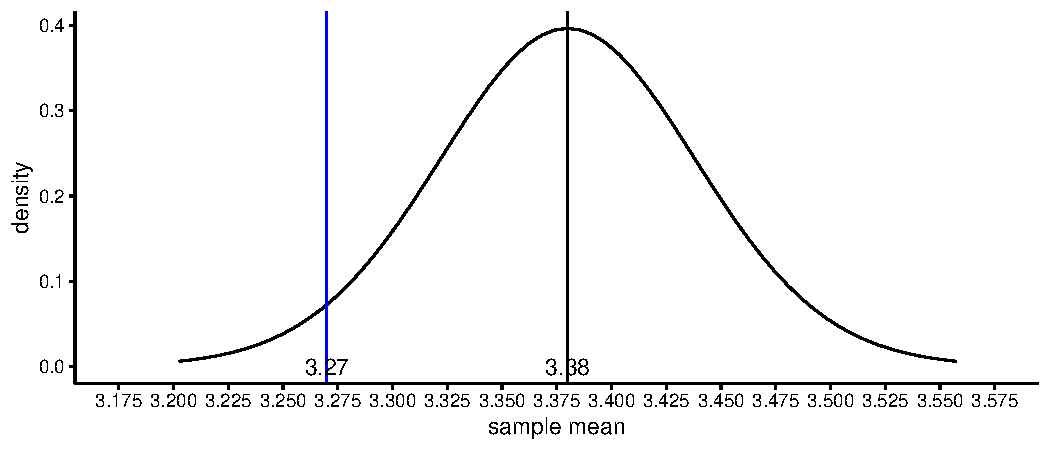
\includegraphics[width=\maxwidth]{figure/hypothesis_test_unstandardised-1} 

}

\caption[The sampling distribution under the null-hypothesis that the South-African population mean is 3.38]{The sampling distribution under the null-hypothesis that the South-African population mean is 3.38. The blue line represents the sample mean for our observed sample mean of 3.27.}\label{fig:hypothesis_test_unstandardised}
\end{figure}


\end{knitrout}


\begin{knitrout}
\definecolor{shadecolor}{rgb}{0.969, 0.969, 0.969}\color{fgcolor}\begin{figure}

{\centering 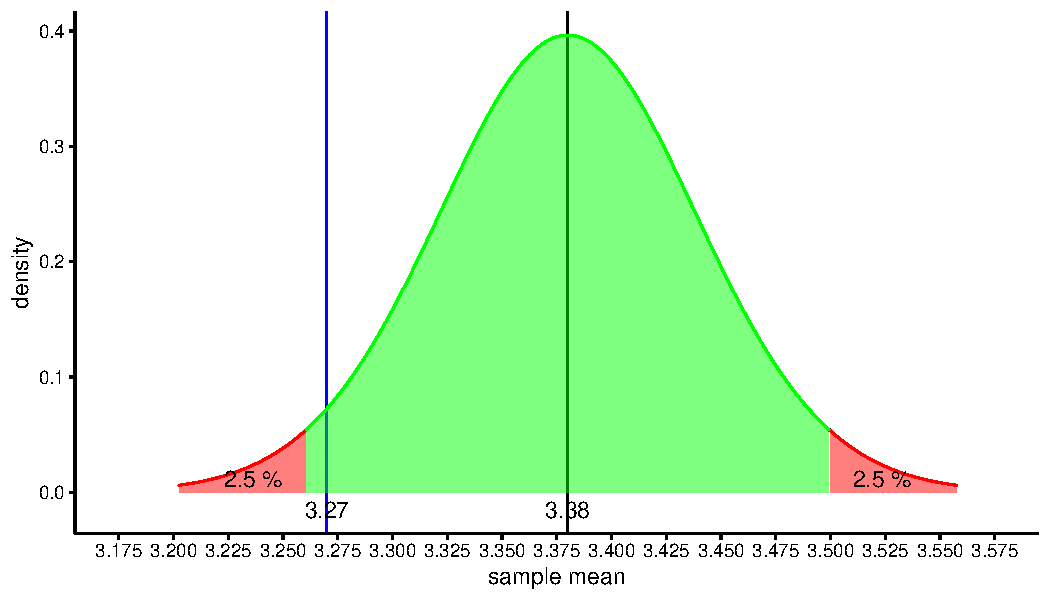
\includegraphics[width=\maxwidth]{figure/hypothesis_test_unstandardised_rejection-1} 

}

\caption[The sampling distribution under the null-hypothesis that the South-African population mean is 3.38]{The sampling distribution under the null-hypothesis that the South-African population mean is 3.38. The red area represents the range of values for which the null-hypothesis is rejected (rejection region), the green area represents the range of values for which the null-hypothesis is not rejected (acceptance region).}\label{fig:hypothesis_test_unstandardised_rejection}
\end{figure}


\end{knitrout}



\section{Null-hypothesis testing with $t$-values}

In the above example, we looked explicitly at the sampling distribution for a hypothesised value for the population mean. By determining what the distribution would look like (determining the mean, standard error and degrees of freedom), we could see whether a certain sample mean would give enough evidence to reject the null-hypothesis. 

In this section we will show how to do this hypothesis testing more easily by first standardising the problem. The trick is that we do not have to make a picture of the sampling distribution every time we want to do a null-hypothesis test. We simply know that its shape is that of a $t$-distribution with degrees of freedom equal to $n-1$. $t$-distributions are standardised distributions, always with a mean of 0. They are the distribution of standardised $t$-statistics, where a sample mean is standardised by subtracting the population mean and dividing the result by the standard error. 

Let's do this standardisation for our observed sample mean of 3.27. With a population mean of 3.38 and a standard error of $\hat{\sigma}_{\bar{y}} = \sqrt{\frac{s^2}{n}} = \sqrt{\frac{0.14}{40}} = 0.059$, we obtain:



\begin{equation}
t = \frac{3.27-3.38}{0.059} = -1.864
\end{equation}



We can then look at a $t$-distribution of $40-1 = 39$ degrees of freedom to see how likely it is that we find such a $t$-score if the null-hypothesis is true. The $t$-distribution with 39 degrees of freedom is depicted in Figure \ref{fig:t-test}. Again we see the population mean represented, now standardised to a $t$-score of 0 (why?), and the observed sample mean, now standardised to a $t$-score of -1.864. As you can see, this graph gives you the same information as the sampling distribution in Figure \ref{fig:hypothesis_test_unstandardised_rejection}. The advantage of using standardisation and using the $t$-distribution is that we can now easily determine whether or not an observed sample mean is somewhere in the red zone or in the green zone, without making a picture. 

We have to find the point in the $t$-distribution where the red and green zones meet. These points in the graph are called \textit{critical values}. From Figure \ref{fig:t-test} we can see that these critical values are around -2 and 2. But where exactly? This information can be looked up in the $t$-tables that were discussed earlier in this chapter. We plot such a table again in Table \ref{tab:t_table2}. A larger version is given in Appendix \ref{app:t}. 

In such a table, you can look up the 2.5th percentile. That is, the value for which 2.5\% of the $t$-distribution is equal or smaller. Because we are dealing with a $t$-distribution with 39 degrees of freedom, we look in the column t39, and then in the row with cumulative probability 0.025 (equal to 2.5\%), we see a value of -2.02. This is the critical value for the lower tail of the $t$-distribution. To find the critical value for the upper tail of the distribution, we have to know how much of the distribution is lower than the critical value. We know that 2.5\% is higher, so it must be the case that the rest of the distribution, $100-2.5 = 97.5$\% is lower than that value. This is the same as a probability of 0.975. If we look for the critical value in the table, we see that it is 2.02. Of course this is the opposite of the other critical value, because the $t$-distribution is symmetrical. 

Now that we know that the critical values are -2.02 and +2.02, we know that for our standardised $t$-score of -1.864 we are still in the green area, so we do not reject the null-hypothesis. We don't need to draw the distribution any more. For any value, we can directly compare it to the critical values. And not only for this example of 40 elephants and a sample mean of 3.27, but for any combination. 

Suppose for example that we would have had a sample size of 10 elephants, and we would have found a sample mean of 3.28 with a slightly different sample variance, $s^2 = 0.15$. If we want to test the null-hypothesis again that the population mean is 3.38 based on these results, we would have to do the following steps:

\bigskip

\noindent\fbox{%
    \parbox{\textwidth}{%
\textbf{Null-hypothesis testing}
\begin{enumerate}
\item Estimate the standard error $\hat{\sigma}_{\widebar{Y}} = \sqrt{\frac{s^2}{n}}$.
\item Calculate the $t$-statistic $t =  \frac{\widebar{Y} - \mu}{\hat{\sigma}_{\widebar{Y}}}$, $\mu$ is the population mean under the null-hypothesis.
\item Determine the degrees of freedom, $n - 1$.
\item Determine the critical values for lower and upper tail of the appropriate $t$-distribution, using Appendix \ref{app:t}.
\item If the $t$-statistic is between the two critical values, then we're in the green, we still believe the null-hypothesis is plausible.
\item If the $t$-statistic is not between the two critical values, we are in the red zone and we reject the null-hypothesis. 
\end{enumerate}

}}

\bigskip



So let's do this for our hypothetical result:

\begin{enumerate}
\item Estimate the standard error: $\sqrt{\frac{0.15}{10}} = 0.1224745$
\item Calculate the $t$-statistic: $t = \frac{3.28-3.38}{0.1224745} = -0.8164966$
\item Determine the degrees of freedom: sample size minus 1 equals 9
\item In Table \ref{tab:t_table2} we look for the row with probability 0.025 and the column for t9. We see a value of -2.26. The other critical value then must be 2.26.
\item The $t$-statistic of -0.8164966 lies between these two critical values, so these sample data do not lead to a rejection of the null-hypothesis that the population mean is 3.38. In other words, these data from 10 elephants do not give us reason to doubt that the population mean is 3.38.

\end{enumerate}




\begin{knitrout}
\definecolor{shadecolor}{rgb}{0.969, 0.969, 0.969}\color{fgcolor}\begin{figure}

{\centering 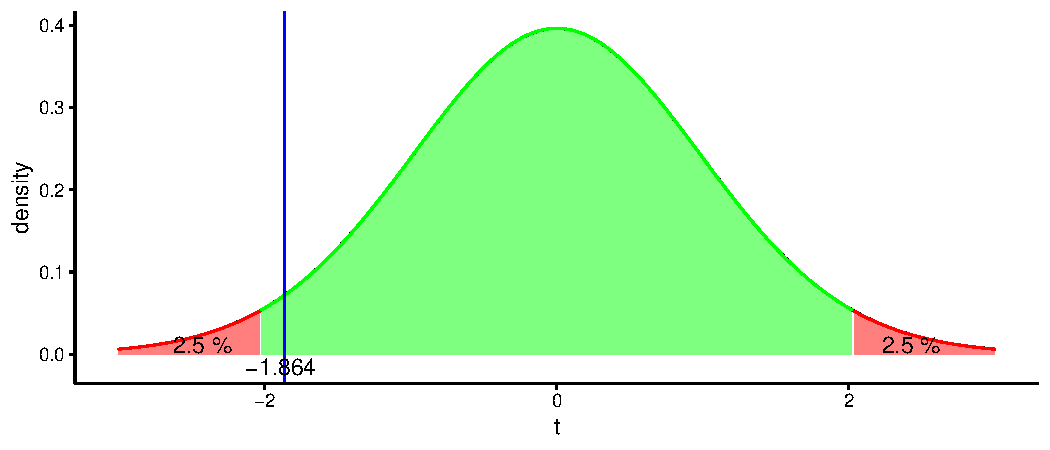
\includegraphics[width=\maxwidth]{figure/t-test-1} 

}

\caption{A \textit{t}-distribution with 39 degrees of freedom to test the null-hypothesis that the South-African population mean is 3.38. The blue line represents the \textit{T}-score for our observed sample mean of 3.27.}\label{fig:t-test}
\end{figure}


\end{knitrout}


% latex table generated in R 4.0.3 by xtable 1.8-4 package
% Sun Jan 31 16:37:12 2021
\begin{table}[ht]
\centering
\caption{Quantiles for the standard normal and several $t$-distributions.} 
\label{tab:t_table2}
\begin{tabular}{rrrrrrrrr}
  \hline
probs & norm & t199 & t99 & t47 & t39 & t9 & t5 & t3 \\ 
  \hline
0.0005 & -3.29 & -3.34 & -3.39 & -3.51 & -3.56 & -4.78 & -6.87 & -12.92 \\ 
  0.0010 & -3.09 & -3.13 & -3.17 & -3.27 & -3.31 & -4.30 & -5.89 & -10.21 \\ 
  0.0050 & -2.58 & -2.60 & -2.63 & -2.68 & -2.71 & -3.25 & -4.03 & -5.84 \\ 
  0.0100 & -2.33 & -2.35 & -2.36 & -2.41 & -2.43 & -2.82 & -3.36 & -4.54 \\ 
  0.0250 & -1.96 & -1.97 & -1.98 & -2.01 & -2.02 & -2.26 & -2.57 & -3.18 \\ 
  0.0500 & -1.64 & -1.65 & -1.66 & -1.68 & -1.68 & -1.83 & -2.02 & -2.35 \\ 
  0.1000 & -1.28 & -1.29 & -1.29 & -1.30 & -1.30 & -1.38 & -1.48 & -1.64 \\ 
  0.9000 & 1.28 & 1.29 & 1.29 & 1.30 & 1.30 & 1.38 & 1.48 & 1.64 \\ 
  0.9500 & 1.64 & 1.65 & 1.66 & 1.68 & 1.68 & 1.83 & 2.02 & 2.35 \\ 
  0.9750 & 1.96 & 1.97 & 1.98 & 2.01 & 2.02 & 2.26 & 2.57 & 3.18 \\ 
  0.9900 & 2.33 & 2.35 & 2.36 & 2.41 & 2.43 & 2.82 & 3.36 & 4.54 \\ 
  0.9950 & 2.58 & 2.60 & 2.63 & 2.68 & 2.71 & 3.25 & 4.03 & 5.84 \\ 
  0.9990 & 3.09 & 3.13 & 3.17 & 3.27 & 3.31 & 4.30 & 5.89 & 10.21 \\ 
  0.9995 & 3.29 & 3.34 & 3.39 & 3.51 & 3.56 & 4.78 & 6.87 & 12.92 \\ 
   \hline
\end{tabular}
\end{table}




\section{The $p$-value}\label{sec:p-values}

What we saw in the previous section was the classical null-hypothesis testing procedure: calculating a $t$-statistic and determine whether or not this $t$-score is in the red zone or green zone, by comparing them to critical values. In the old days, this was done by hand: the calculation of $t$ and looking up the critical values in tables published in books.

These days we have the computer do the work for us. If you have a data set, a program can calculate the $t$-score for you. However, when you look at the output, you actually never see whether this $t$-score leads to  a rejection of the null-hypothesis or not. The only thing that a computer prints out is the $t$-score, the degrees of freedom, and a so-called $p$-value. In this section we explain what a $p$-value is and how you can use it for null-hypothesis testing.


Let's go back to our example in the previous section, where we found a sample mean height of 3.28 with only 10 elephants. We computed the $t$-score and obtained -0.82. We illustrate this result in Figure \ref{fig:p-value} where the red line indicates the $t$-score. By comparing this $t$-value with the critical values, we could decide that we do not reject the null-hypothesis. However, if you would do this calculation with a computer program like R, we would get the following result:

\begin{lstlisting}
t = -0.82, df = 9, p-value = 0.434
\end{lstlisting}



\begin{knitrout}
\definecolor{shadecolor}{rgb}{0.969, 0.969, 0.969}\color{fgcolor}\begin{figure}

{\centering 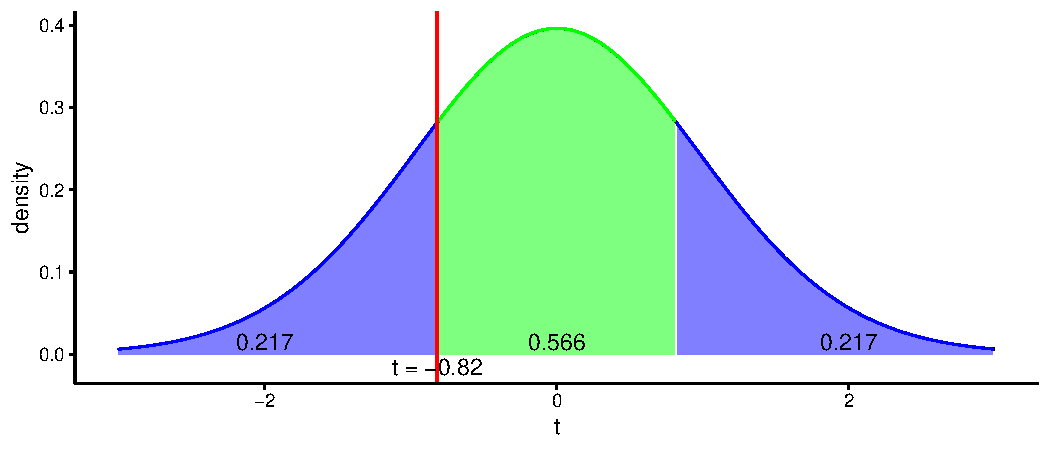
\includegraphics[width=\maxwidth]{figure/p-value-1} 

}

\caption[Illustration of what a $p$-value is]{Illustration of what a $p$-value is. The total blue area represents the probability that under the null-hypothesis, you find a more extreme value than the $t$-score or its opposite. The blue area covers a proportion of .217 + .217 = .434 of the $t$-distribution. This amounts to a $p$-value of .434.}\label{fig:p-value}
\end{figure}


\end{knitrout}


Figure \ref{fig:p-value} shows what this $p$-value of 0.434 means. The green area in the middle represents the probability that a $t$-score lies between -0.82 and +0.82. That probability is shown in the figure as 0.567, so 56.7\%. The left blue region represents the probability that if the null-hypothesis is true, the $t$-score will be less than -0.82. That probability is 0.217, so 21.7\%. Because of symmetry, the probability that the $t$-score is more than 0.82 is also 0.217. The blue regions together therefore represent the probability that you find a $t$-score of less than -0.82 or more than 0.82, and that probability equals 0.217 + 0.217 = 0.434. Therefore, the probability that you find a $t$-value of $\pm 0.82$ or more extreme equals 0.434. This probability is called the $p$-value. 

Why is this value useful?


Let's imagine that we find a $t$-score of exactly equal to one of the critical values. The critical value for a sample size of 10 animals related to a cumulative proportion of 0.025 equals -2.26 (see Table \ref{tab:t_table2}). Based on this table, we know that the probability of a $t$-value of -2.26 or lower equals 0.025. Because of symmetry, we also know that the probability of a $t$-value of 2.26 or higher also equals 0.025. This brings us to the conclusion that the probability of a $t$-score of $\pm 2.26$ or more extreme, is equal to $0.025+0.025 = 0.05 = 5\%$. Thus, when the $t$-score is equal to the critical value, then the $p$-value is equal to 5\%. You can imagine that if the $t$-score becomes more extreme than the critical value the $p$-value will become less than 5\%, and if the $t$-score becomes less extreme (closer to 0), the $p$-value becomes larger.

In the previous section, we said that if a $t$-score is more extreme than one of the critical values (i.e., when it doesn't have a value between them) then we reject the null-hypothesis. Thus, a $p$-value of 5\% or less means that we have a $t$-score more extreme than the critical values, which in turn means we have to reject the null-hypothesis. Thus, based on the computer output, we see that the $p$-value is larger than 0.05, so we do not reject the null-hypothesis.


\bigskip



\noindent\fbox{%
    \parbox{\textwidth}{%
\textbf{Overview}
\begin{itemize}



\item critical value: the minimum (or maximum) value that a $t$-score should have to be in the red zone (the rejection region). If a $t$-value is more extreme than a critical value, then the null-hypothesis is rejected. The red zone is often chosen such that a $t$-score will be in that zone 5\% of the time, assuming that the null-hypothesis is true.

\item $p$-value: indicates the probability of finding a $t$-value equal or more extreme than the one found, assuming that the null-hypothesis is true. Often a $p$-value of 5\% or smaller is used to support the conclusion that the null-hypothesis is not tenable. This is equivalent to a rejection region of 5\% when using critical values.


\end{itemize}

}
}
\bigskip


Let's apply this null-hypothesis testing to our luteinising hormone (LH) data. Based on the medical literature, we know that LH levels for women in their child-bearing years vary between 0.61 and 56.6 IU/L. Values vary during the menstrual period. If values are lower than normal, this can be an indication that the woman suffers from malnutrition, anorexia, stress or a pituitary disorder. If the values are higher, this is an indication that the woman has gone through menopause.

We're going to use the LH data presented earlier in this chapter to make a decision whether the woman has a healthy range of values for a woman in her child-bearing years by testing the null-hypothesis that the mean LH level in this woman is the same as the mean of LH levels in healthy non-menopausal women.

First we specify the null-hypothesis. Suppose we know that the mean LH level in this woman should be equal to 2.54, given her age and given the timing of her menstrual cycle. Thus our null-hypothesis is that the mean LH in our particular woman is equal to 2.54:


\begin{equation}
H_0: \mu = 2.54
\end{equation}


Next, we look at our sample mean and see whether this is a likely or unlikely value to find under this null-hypothesis. The sample mean is 2.40. To know whether this is a likely value to find, we have to know the standard error of the sampling distribution, and we can estimate this by using the sample variance. The sample variance $s^2 = 0.3042553$ and we had 48 measures, so we estimate the standard error as $\hat{\sigma}_{\bar{y}} = \sqrt{\frac{s^2}{n}} = \sqrt{\frac{0.3042553}{48}} = 0.08$. We then apply standardisation to get a $t$-value:

\begin{equation}
t = \frac{2.40 - 2.54}{0.08} = -1.75 
\end{equation}

Next, we look up in a table whether this $t$-value is extreme enough to be considered unlikely under the null-hypothesis. In Table \ref{tab:t_table2}, we see that for 47 degrees of freedom, the critical value for the 0.025 quantile equals -2.01. For the 0.975 quantile it is 2.01. Our observed $t$-value of -1.75 lies within this range. This means that a sample mean of 2.40 is likely to be found when the population mean is 2.54, so we do not reject the null-hypothesis. We conclude that the LH levels are healthy for a woman her age.  

When we report the results from a null-hypothesis test, we often talk about \textit{significance}. When the results show that the null-hypothesis can be rejected, we talk about a \textit{statistically significant} result. When the null-hypothesis cannot be rejected, we call the results non-significant. Note that this says nothing about the importance or size of the results.   

In a report, you could state:

\begin{quotation}
"We tested the null-hypothesis that the mean LH level is 2.54. Taking a sample of 48 measurements, we obtained a mean of 2.40. A $t$-test showed that this sample mean was not significantly different from 2.54, $t(47) = -1.75, p > .05$."
\end{quotation}




We can do the null-hypothesis testing also with a computer. Let's analyse the data in R and do the computations with the following code. First we load the LH data:


\begin{knitrout}
\definecolor{shadecolor}{rgb}{0.969, 0.969, 0.969}\color{fgcolor}\begin{kframe}
\begin{alltt}
\hlkwd{data}\hlstd{(lh)}
\end{alltt}
\end{kframe}
\end{knitrout}

Next, we test whether the population mean could be 2.54:

\begin{knitrout}
\definecolor{shadecolor}{rgb}{0.969, 0.969, 0.969}\color{fgcolor}\begin{kframe}
\begin{alltt}
\hlkwd{t.test}\hlstd{(lh,} \hlkwc{mu} \hlstd{=} \hlnum{2.54}\hlstd{)}
\end{alltt}
\begin{verbatim}
## 
## 	One Sample t-test
## 
## data:  lh
## t = -1.7584, df = 47, p-value = 0.08518
## alternative hypothesis: true mean is not equal to 2.54
## 95 percent confidence interval:
##  2.239834 2.560166
## sample estimates:
## mean of x 
##       2.4
\end{verbatim}
\end{kframe}
\end{knitrout}


In the output we see that the $t$-value is equal to -1.7584, similar to our -1.75. We see that the number of degrees of freedom is 47 ($n-1$) and that the $p$-value equals 0.08518. This $p$-value is larger than 0.05, so we do \textit{not} reject the null-hypothesis that the mean LH level in this woman equals 2.54. Her LH level is healthy.

In a report, the convention is to report the exact $p$-value. We can omit the 0 in front of the decimal sign since a $p$-value is always between 0 and 1 (i.e., .09 instead of 0.09)

\begin{quotation}
"We tested the null-hypothesis that the mean LH level is 2.54. Taking a sample of 48 measurements, we obtained a mean of 2.40. A $t$-test showed that this sample mean was not significantly different from 2.54, $t(47) = -1.75, p = .09$."
\end{quotation}

\section{One-sided versus two-sided testing}

In the previous section, we tested a null-hypothesis in order to find evidence that an observed sample mean was either too large or too small to result from random sampling. For example, in the previous section we saw that the observed LH levels were not too low and we did not reject the null-hypothesis. But had the LH levels been too high or too low, then we would have rejected the null-hypothesis. 


In the reasoning that we followed, there were actually two hypotheses: the null-hypothesis that the population mean was exactly 2.54, and the \textit{alternative hypothesis} that the population is not exactly 2.54:

\begin{eqnarray}
H_0: \mu = 2.54 \\
H_A: \mu \neq 2.54
\end{eqnarray}


This kind of null-hypothesis testing is called \textit{two-sided} or \textit{two-tailed} testing: we look at two critical values, and if the computed $t$-score is outside this range (i.e., somewhere in the two tails of the distribution), we reject the null-hypothesis.

The alternative to two-sided testing is \textit{one-sided} or \textit{one-tailed} testing. Sometimes before an analysis you already have an idea of what direction the data will go. For instance, imagine a zoo where they have held elephants for years. These elephants always were of Tanzanian origin, with a mean height of 3.38. Lately however, the manager observes that the opening that connects the indoor housing with the outdoor housing gets increasingly damaged. Since the zoo recently acquired 4 new elephants of South-African origin, the manager wonders whether South-African elephants are on average taller than the Tanzanian elephants. 
To figure out whether South-African elephants are on average taller than the Tanzanian average of 3.38 or not, the manager decides to apply null-hypothesis testing. She has two hypotheses: null-hypothesis $H_0$ and \textit{alternative hypothesis} $H_A$:

\begin{eqnarray}
H_0: \mu_{SA} = 3.38 \\
H_A: \mu_{SA} > 3.38
\end{eqnarray}

This set of hypotheses leaves out one option: the South-African mean might be lower than the Tanzanian one. Therefore, one often writes the set of hypotheses like this:

\begin{eqnarray}
H_0: \mu_{SA} \leq 3.38 \\
H_A: \mu_{SA} > 3.38
\end{eqnarray}


She next tests the null-hypothesis, more specifically the one where $\mu_{SA} = 3.38$. From the damaged doorway she expects the sample mean to be higher than 3.38, but is it high enough to serve as evidence that the population mean is also higher than 3.38? She decides that when the sample mean is in the rejection zone in the right tail of the sampling distribution, then she will decide that the null-hypothesis is not true, but that the alternative hypothesis must be true. 

This is illustrated in Figure \ref{fig:hypothesis_test_unstandardised_rejection_onetailed}. It shows the sampling distribution if we happen to have 4 new South-African elephants, with a sample mean of 3.45 and a standard error of 0.059. In red, we see the rejection region: if the sample mean happens to be in that zone we decide to reject the null-hypothesis. Similar to two-tailed testing, we decide that an area of 5\% is small enough to suggest that the null-hypothesis is not true. Note that in two-tailed testing, this area of 5\% was divided equally into the upper tail and the lower tail of the distribution, but with one-tailed testing we put it all in the tail where we expect to find the sample mean based on a theory or a hunch.

In this sampling distribution, based on 3 degrees of freedom, we see that the sample mean is not in the red zone -- the rejection region -- therefore we do not reject the null-hypothesis. We conclude that based on this random sample of 4 elephants, there is no evidence to suggest that South-African elephants are on average taller than Tanzanian elephants.


\begin{knitrout}
\definecolor{shadecolor}{rgb}{0.969, 0.969, 0.969}\color{fgcolor}\begin{figure}

{\centering 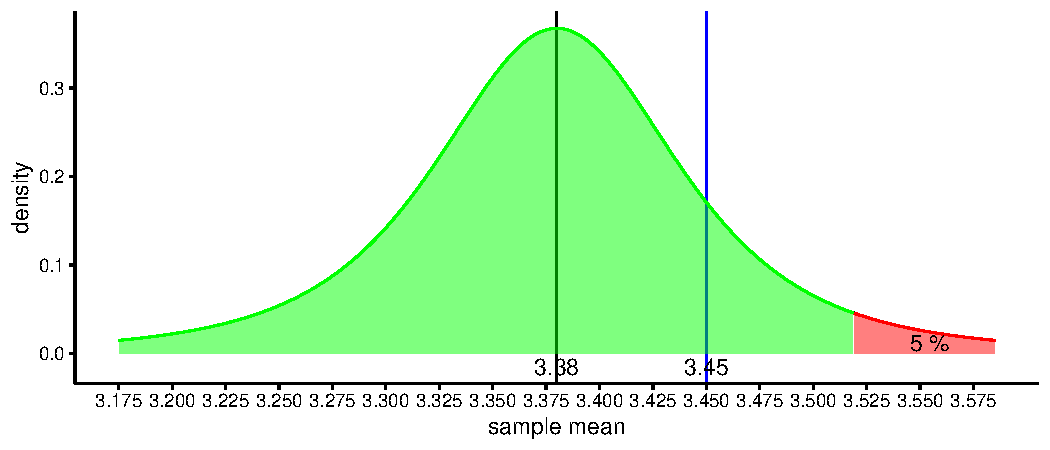
\includegraphics[width=\maxwidth]{figure/hypothesis_test_unstandardised_rejection_onetailed-1} 

}

\caption[The sampling distribution under the null-hypothesis that the South-African population mean is 3.38]{The sampling distribution under the null-hypothesis that the South-African population mean is 3.38. In one-tailed testing, the rejection area is located in only one of the tails. The red area represents the range of values for which the null-hypothesis is rejected (rejection region), the green area represents the range of values for which the null-hypothesis is not rejected (acceptance region).}\label{fig:hypothesis_test_unstandardised_rejection_onetailed}
\end{figure}


\end{knitrout}


The same procedure can be done with standardisation. We compute the $t$-statistic as 

\begin{equation}
t = \frac{3.45 - 3.38}{0.059} = 1.19 
\end{equation}

In Table \ref{tab:t_table2} we have to look up where the red zone starts: that is for the 0.95 quantile, because below that value lies 95\% (green zone) and above it 5\% (the red zone). We see that the 95th percentile for a $t$-distribution with 3 degrees of freedom is equal to 2. Our $t$-value 1.19 is less than that, so that we do not reject the null-hypothesis. 

A third way is to compute a one-tailed $p$-value. This is illustrated in Figure \ref{fig:p_value_onetailed}. The one-tailed $p$-value for a $t$-statistic of 1.19 and 3 degrees of freedom turns out to be 0.16. That is the proportion of the $t$-distribution that is blue. That means that if the null-hypothesis is true, you will find a $t$-value of 1.19 or larger in 16\% of the cases. Because this proportion is more than 5\%, we do not reject the null-hypothesis.



\begin{knitrout}
\definecolor{shadecolor}{rgb}{0.969, 0.969, 0.969}\color{fgcolor}\begin{figure}

{\centering 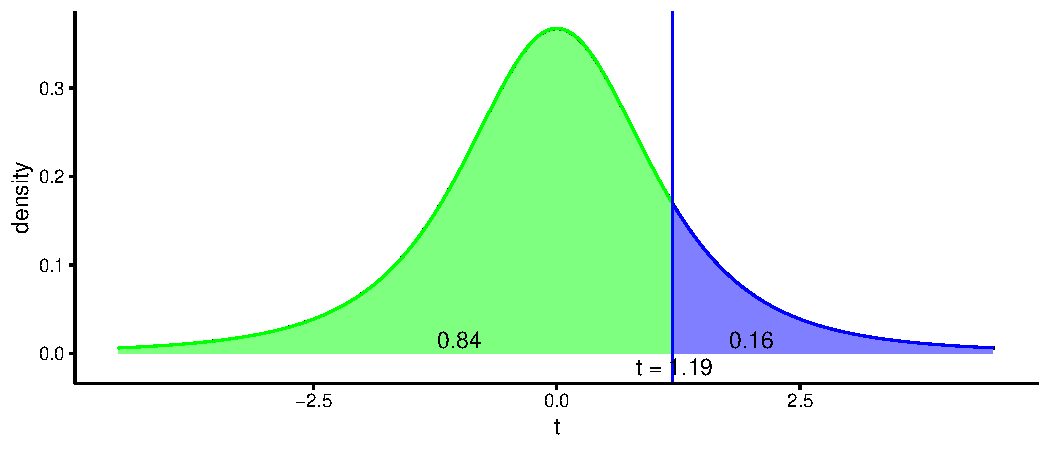
\includegraphics[width=\maxwidth]{figure/p_value_onetailed-1} 

}

\caption[The sampling distribution under the null-hypothesis that the South-African population mean is 3.38]{The sampling distribution under the null-hypothesis that the South-African population mean is 3.38. For one-tailed testing, the rejection area is located in only one of the tails. The green area represents the probability of seeing a $t$-value smaller than 1.19, the blue are represents the probability of seeing a $t$-value larger than 1.19. The latter probability is the $p$-value.}\label{fig:p_value_onetailed}
\end{figure}


\end{knitrout}


\section{One-tailed testing applied to LH levels}


As we have seen, LH levels that are too high are indicative of menopause, a normal transition for women. However, LH levels that are too low are indicative of an illness or malnutrition. In that case, it is important that the source of this malnutrition or the specific illness is diagnosed. You could therefore say that if LH levels are too low, a red flag should be put up, whereas if the LH levels are normal or higher, then there is usually no reason to worry. 

LH levels can therefore be used to construct a diagnostic red flag decision system. If normal or high, then nothing happens, if too low, then something should be done. We could formulate these two alternative states of reality as two hypotheses:


\begin{eqnarray}
H_0: \mu_{LH} \geq 2.54 \\
H_A: \mu_{LH} <  2.54
\end{eqnarray}

We decide beforehand that if a $t$-value is too far out in the left tail of the distribution, the LH levels are too low. We again use 5\% of the area of the $t$-distribution. This decision process is illustrated in Figure \ref{fig:LH_one-tailed} where we see a critical $t$-value of -1.68 when we we have 47 degrees of freedom (see Table \ref{tab:t_table2}). 


\begin{knitrout}
\definecolor{shadecolor}{rgb}{0.969, 0.969, 0.969}\color{fgcolor}\begin{figure}
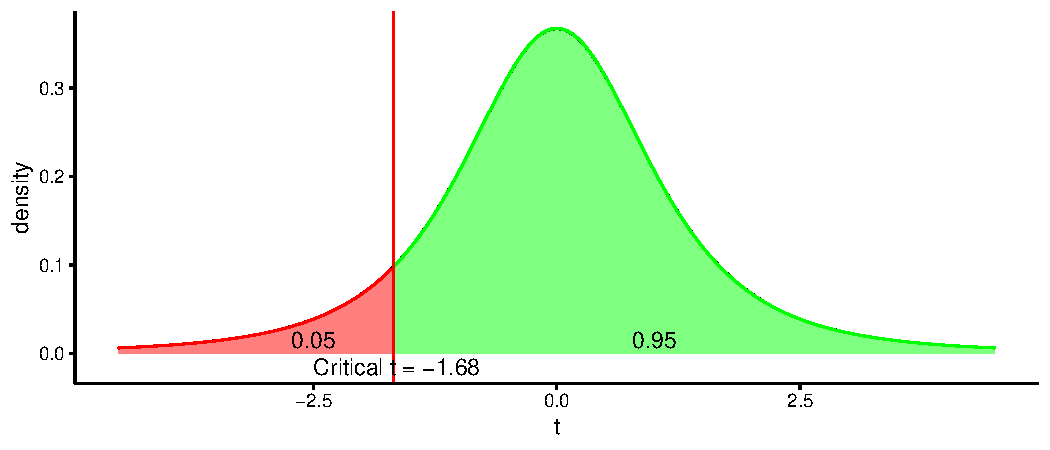
\includegraphics[width=\maxwidth]{figure/LH_one-tailed-1} \caption[One-tailed decision process for deciding whether the average LH level in a woman is too low]{One-tailed decision process for deciding whether the average LH level in a woman is too low.}\label{fig:LH_one-tailed}
\end{figure}


\end{knitrout}


We calculate our $t$-value and find -1.75, see section \ref{sec:p-values}. We see that this $t$-value is smaller than the critical value -1.68, so it is in the red rejection area. This is the area that we use for the rejection of the null-hypothesis, so based on these data we decide that the mean LH level in this woman is abnormally low. 


Importantly, note that when we applied two-tailed hypothesis testing, we decided to \textit{not} reject the null-hypothesis, whereas here with one-tailed testing, we decide to reject the null-hypothesis. All based on the same data, and the same null-hypothesis. The difference lies in the choice of the alternative hypothesis. When doing one-tailed testing, we put all of the critical region in only one tail of the $t$-distribution. This way, it becomes easier to reject a null-hypothesis, if the mean LH level is indeed lower than normal. However, it could also be easier to make a mistake: if the mean LH level is in fact normal, we could make a mistake in thinking that the sample mean is deviant, where it is actually not. Making mistakes in inference is the topic of the next section.

It is generally advised to use two-tailed testing rather than one-tailed testing. The reason is that in hypothesis testing, it is always the null-hypothesis that is being used as the starting point: what would the sample means (or their standardised versions: $t$-scores) look like if the null-hypothesis is true? Based on a certain null-hypothesis, say population mean $\mu$ equals 2.54, sample means could be as likely higher or lower than the population mean (since the sampling distribution is symmetrical). Even if you suspect that $\mu$ is actually lower, based on a very good theory, you would help yourself too much to falsify the null-hypothesis by putting the rejection area only in the left tail of the distribution. And what do you actually do if you find a sample mean that is in the far end of the right tail? Do you still accept the null-hypothesis? That would not make much sense. It is therefore better to just stick to the null-hypothesis, and see whether the sample mean is far enough removed to reject the null-hypothesis. If the sample mean is in the anticipated tail of the distribution, that supports the theory you had, and if the sample mean is in the opposite tail, it does not support the theory you had. 

Compare one-tailed and two-tailed testing in R using the LH data. By default, R applies two-tailed testing. R gives the following output:

\begin{knitrout}
\definecolor{shadecolor}{rgb}{0.969, 0.969, 0.969}\color{fgcolor}\begin{kframe}
\begin{alltt}
\hlkwd{t.test}\hlstd{(lh,} \hlkwc{mu} \hlstd{=} \hlnum{2.54}\hlstd{)}
\end{alltt}
\begin{verbatim}
## 
## 	One Sample t-test
## 
## data:  lh
## t = -1.7584, df = 47, p-value = 0.08518
## alternative hypothesis: true mean is not equal to 2.54
## 95 percent confidence interval:
##  2.239834 2.560166
## sample estimates:
## mean of x 
##       2.4
\end{verbatim}
\end{kframe}
\end{knitrout}

If you want one-tailed testing, where you expect that the mean LH level is lower than 2.54, you do that in the following manner\footnote{If you expect that the LH level will higher than 2.54, you use "greater" instead of "less".}:

\begin{knitrout}
\definecolor{shadecolor}{rgb}{0.969, 0.969, 0.969}\color{fgcolor}\begin{kframe}
\begin{alltt}
\hlkwd{t.test}\hlstd{(lh,} \hlkwc{mu} \hlstd{=} \hlnum{2.54}\hlstd{,} \hlkwc{alternative} \hlstd{=} \hlstr{"less"}\hlstd{)}
\end{alltt}
\begin{verbatim}
## 
## 	One Sample t-test
## 
## data:  lh
## t = -1.7584, df = 47, p-value = 0.04259
## alternative hypothesis: true mean is less than 2.54
## 95 percent confidence interval:
##      -Inf 2.533589
## sample estimates:
## mean of x 
##       2.4
\end{verbatim}
\end{kframe}
\end{knitrout}

With one-tailed testing, you can report:

\begin{quotation}
"We tested the null-hypothesis that the mean LH level is 2.54, against the alternative hypothesis that the mean LH level is less than 2.54. Taking a sample of 48 measurements, we obtained a mean of 2.40. A one-tailed $t$-test showed that this sample mean was significantly less than 2.54, $t(47) = -1.75, p = .04$."
\end{quotation}



When you compare the $p$-values, you see that the $p$-value using one-tailed testing is half the size of the $p$-value using two-tailed testing (.04259 vs .08518). Based on the previous sections, you should know why the $p$-value is halved! (Because the $t$-distribution is symmetrical and you placed all of the 5\% rejection area only on the left of the $t$-distribution). In the second output, using a critical $p$-value of 5\% you would reject the null-hypothesis, whereas in the first output, you would not reject the null-hypothesis. Using one-tailed testing could lead to a big mistake: thinking that the sample mean is deviant enough to reject the null-hypothesis, while the null-hypothesis is actually true. We delve deeper into such mistakes in the next section. 


% 105.	Type I and type II errors (required unit)
% 





% •	Can explain what is meant by a type I error and a type II error.
% •	Can perform null-hypothesis test on the basis of a confidence interval.
% •	Can perform a one-sample t-test in R, find the confidence interval, interpret the p-value.
% 
% •	Given sample mean and sample variance, can compute various confidence intervals for the population mean, (by looking up various critical t-values in a table). 
% 
%

\section{Type I and type II errors}

In the preceding sections, we have used the value of 5\% a lot of times. We deemed that this was a fairly low probability, that allows us to take the decision to reject the null-hypothesis. We looked at the distribution of sample means, given that there was a certain population mean, and we looked at how often we can expect a sample mean that is smaller or larger than certain critical values. These critical values were based on 5\% of the area of the sampling distribution. With two-tailed testing, this 5\% was divided over the two extreme tails of the sampling distribution, and with one-tailed testing, this 5\% rejection area was put in the tail end where we expected the population to be according to the alternative hypothesis (based on theory).

In this null-hypothesis testing procedure there is always the risk that we take the wrong decision. Let's return to our elephant example where we had the null-hypothesis that the population mean for South-African elephants equals 3.38. The alternative two-sided hypothesis was that the population mean was \textit{not} equal to 3.38. After calculating the standard error, we calculated the $t$-score. We said that we reject the null-hypothesis when the obtained $t$-score was somewhere in the extreme ends of the tail: more specifically, in the rejection area that made up 5\% of the area of the $t$-distribution. That means that if the null-hypothesis is true, there is a 5\% probability that we find such a $t$-score. In that case we reject the null-hypothesis. But that could be the wrong decision: if the null-hypothesis is true it will happen in 5\% of the cases that a $t$-score will be in the 5\% rejection region. We then reject the null-hypothesis while it is actually true! Such a mistake is called a Type I error. In this case, type I error rate is 5\%. It is a \textit{conditional probability}. Conditional probabilities are probabilities that start from some given information. In this case, the given information is that the null-hypothesis is true: \textit{given} that the null-hypothesis is true, it is the probability that we reject the null-hypothesis. Because we do not like to make mistakes, we want to have the probability of a mistake as low as possible.

In the social and behavioural sciences, one thinks that a probability of 5\% is low enough to take the risk of making the wrong decision. As stated earlier, in quantum mechanics one is even more careful, using a probability of 0.000057 \%. So why don't we also use a much lower probability of making a type I error? The answer is that we do not want to make another type of mistake: a type II error. A type II error is the mistake that we make when we do \textit{not} reject the null-hypothesis, while it is not true. Taking the example of the elephants again, suppose that the population mean is \textit{not} equal to 3.38, but the $t$-score is not in the rejection area, so we believe that the population mean is 3.38. This is then the wrong decision. The type of mistake we then make is a type II error.


Let's take this example further. Suppose we have a two-tailed decision process, where we compare two hypotheses about South-African elephants: either their mean height is equal to 3.38 ($H_0$), or it is not ($H_A$). We compute the $t$-statistic and determine the critical values based on 5\% area in the tails of the $t$-distribution. This means that we allow ourselves to make a mistake in 5\% of the cases: the probability that we find a $t$-score in one of the 2.5\% tails equals 2.5\% + 2.5\% = 5\%. This is the probability of a type I error. Note that we chose this value deliberately. This 5\% we call $\alpha$ ('alpha'): it is the relative frequency we allow ourselves to make a type I error. We say then that our $\alpha$ is fixed to 0.05, or 5\%. This means that if the null-hypothesis is true, the probability that the $t$-statistic will be in in the tails will be 5\%.

Then what is the probability of a type II error? A type II error is based on the premise that the alternative hypothesis is true. That alternative hypothesis states that the population mean is \textit{not} equal to 3.38. Given that, what is the probability that we do not reject the null-hypothesis?

This is impossible to compute, because the alternative hypothesis is very vaguely stated: it could be anything, as long as it is not 3.38. Let's make it a bit easier and state that the alternative hypothesis states that the population mean equals 3.42.


\begin{eqnarray}
H_0: \mu_{SA} = 3.38 \\
H_A: \mu_{SA} =  3.42
\end{eqnarray}




\begin{knitrout}
\definecolor{shadecolor}{rgb}{0.969, 0.969, 0.969}\color{fgcolor}\begin{figure}

{\centering 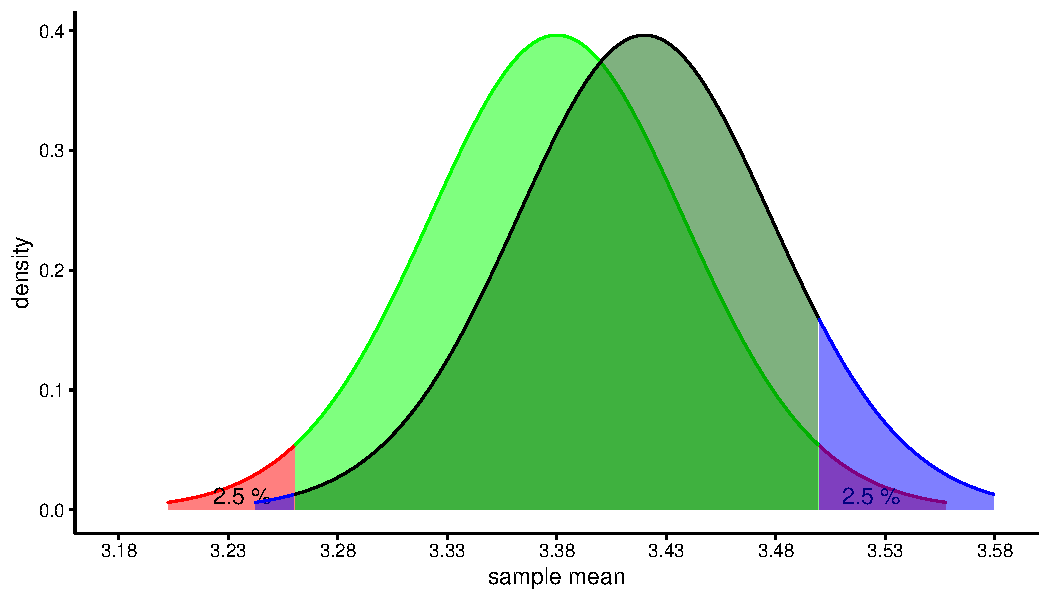
\includegraphics[width=\maxwidth]{figure/type_II_error-1} 

}

\caption[Two sampling distributions, one for a population mean of 3.38 (null-hypothesis) and one for a population mean of 3.42 (alternative hypothesis)]{Two sampling distributions, one for a population mean of 3.38 (null-hypothesis) and one for a population mean of 3.42 (alternative hypothesis). The red areas represent the probability of a type I error, the dark green area the probability of a type II error. The blue areas represent the probability of making the (correct) decision that the null-hypothesis is not true when it is indeed not true.}\label{fig:type_II_error}
\end{figure}


\end{knitrout}


If the population mean height is equal to 3.42, what would sample means look like? That's easy, that is the sampling distribution of the sample mean. The mean of that sampling distribution would be 3.42. This is illustrated in Figure \ref{fig:type_II_error}. The left curve is the sampling distribution for a population mean of 3.38. The red area represents the probability of a type I error. The right curve is the sampling distribution for a population mean of 3.42. The blue area represents the probability of rejecting the null-hypothesis. This is because if the sample mean is smaller than 3.260336 or larger than 3.499664, the sample mean is in the rejection area of the null-hypothesis testing and the null-hypothesis will therefore be rejected. The probability of this happening given that the \textit{alternative} hypothesis is true ($H_A = 3.42$), is represented by the area under that curve: the blue area. If we determine the two blue areas in Figure \ref{fig:type_II_error}, we end up with $0.004 + 0.097 = 0.101$. This is the probability of rejecting the null-hypothesis while it is not true, so this is no mistake at all. We would make a mistake when the alternative hypothesis is true, and we would \textit{not} reject the null-hypothesis. This is represented by the dark green area. That area is equal to 1 minus the blue area: $1- 0.101 = 0.899$.


\begin{knitrout}
\definecolor{shadecolor}{rgb}{0.969, 0.969, 0.969}\color{fgcolor}\begin{figure}

{\centering 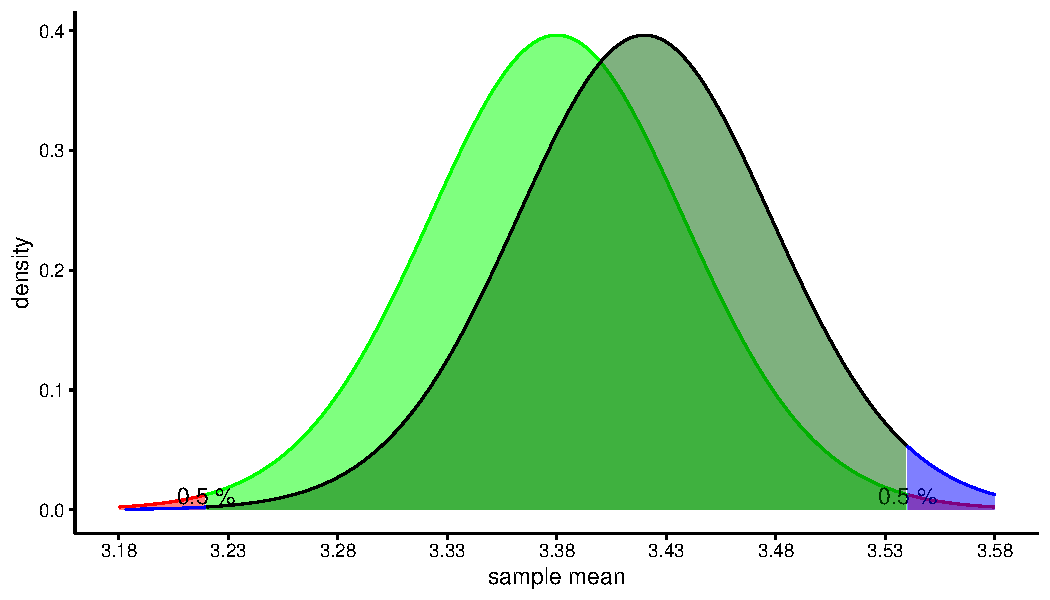
\includegraphics[width=\maxwidth]{figure/type_II_error_2-1} 

}

\caption[Two sampling distributions, one for a population mean of 3.38 (null-hypothesis) and one for a population mean of 3.42 (alternative hypothesis)]{Two sampling distributions, one for a population mean of 3.38 (null-hypothesis) and one for a population mean of 3.42 (alternative hypothesis). The red areas represent the probability of a type I error, the dark green area the probability of a type II error. The blue area represents the probability of making the (correct) decision that the null-hypothesis is not true when it is indeed not true.}\label{fig:type_II_error_2}
\end{figure}


\end{knitrout}



When we have to make a definite decision about a population mean, the null-hypothesis framework can be used for that. Usually we don't want to make type I error mistakes, so we pick a low probability like 5\% for the tails of the sampling distribution under the $H_0$. This value is called $\alpha$: if the null-hypothesis is true, we don't want to reject it, so we allow this to happen in only 5\% of the cases. One chooses $\alpha$ before collecting the data. You have to be careful with this choice of $\alpha$ though because it directly affects the probability of making a type II error. This probability is denoted by $\beta$ ('beta'): how often does it happen that if the alternative hypothesis is true, we do not reject the null-hypothesis. This relationship is illustrated in Figure \ref{fig:type_II_error_2}. There, an $\alpha$ of 1\% is chosen, using both tails (a two-tailed null-hypothesis test). You immediately see that the blue areas have also become smaller, and that by consequence the dark green area becomes larger: the probability of a type II error. 

Thus, the $\alpha$ should be chosen wisely: if it is too large, you run a high risk of a type I error. But if it is too low, you run a high risk of a type II error. Let's think about this in the context of our luteinising hormone problem. 

We saw that if the LH level is low, this could be an indication of malnutrition or a disease and the patient should have further checks to see what the problem is. But if the LH level is normal or above normal, there is no disease and no further checks are required. Again we take the null-hypothesis that the mean LH level in this woman equals 2.54. What would be a type I error in this case, and what would be a type II error?

The type I error is the mistake of rejecting the null-hypothesis while it is in fact true. Thus, the woman's mean LH level is 2.54, but by coincidence, the mean of the 48 measurements that we have turns out to be in the rejection area of the sampling distribution. If this happens we make the mistake that we do a lot of tests with this woman to find out what's wrong with her, while in fact she is perfectly healthy! How bad would such a mistake be? It would certainly lead to extra costs, but also a lot of the woman's time. She would also probably start worrying that something is wrong with her. So we definitely don't want this to happen. We can minimise the risk of a type I error by choosing a low $\alpha$.

The type II error is the mistake of \textit{not} rejecting the null-hypothesis while it is in fact not true. Thus, the woman's mean LH level is lower than 2.54, but by coincidence, the sample mean of the 48 measurements that we have turns out to be in the acceptance area of the sampling distribution. This means that the woman's LH level does not seem to be abnormal, and the woman is sent home. How bad would such a mistake be? Well, pretty bad because the woman's hormone level is not normal, but everybody thinks that she is OK. She could be very ill but nothing is found in further tests, because there are no further tests. So we definitely don't want this to happen. We can minimise the risk of a type II error by choosing a higher $\alpha$.

So here we have a conflict, and we have to make a balanced choice for $\alpha$: too low we run the risk of type II errors, too high we run the risk of a type I error. Then you have to decide what is worse: a type I mistake or a type II mistake. In this case, you could defend that sending the woman home while she is ill, is worse than spending money on tests that are actually not needed. Then you would choose a rather high $\alpha$, say 10\%. That means that if you have several women who are in fact healthy, 10\% of them would receive extra testing. This is a fairly high percentage, but you are more sure that women with an illness will be detected and receive proper care. 

But if you think it is most important that you don't spend too much money and that you don't want women to start worrying when it is not needed, you can pick a low $\alpha$ like 1\%: then when you have a lot of healthy women, only 1\% of them will receive unnecessary testing.




\bigskip



\noindent\fbox{%
    \parbox{\textwidth}{%
\textbf{Overview}
\begin{itemize}

\item \textbf{Type I error}: the mistake of rejecting the null-hypothesis, while it is true

\item \textbf{Type II error}: the mistake of not rejecting the null-hypothesis, while it is not true


\item \textbf{$\alpha$}: the relative frequency we allow ourselves to make a type I error

\item \textbf{$\beta$}: the relative frequency of making a type II error

\end{itemize}

}%
}


\bigskip












% 106.	Inference for a proportion (optional unit)
% 
% •	Can compute the standard error for a proportion.
% •	Can compute a confidence interval for a proportion.
% •	Can state a null-hypothesis regarding a population proportion.
% •	Can perform a null-hypothesis test by hand concerning a population proportion, a given sample proportion and given sample size on the basis of a table with critical z-values.
% •	Can perform a proportion test in R and interpret the p-value.
% 

 % label mean


\chapter{Inference about a proportion}\label{chap:prop}




\section{Sampling distribution of the sample proportion}



So far, we focused on inference about a population mean: starting from a sample mean, what can we infer about the population mean? However, there are also other sample statistics we could focus on. We briefly touched on the variance in the sample and what it tells us about the population variance. In this section, we focus on inference regarding a proportion. 

Let's go back to the example of the elephants in the zoo, and that the manager saw a damaged doorway. This is most likely caused by elephants that are taller than a certain height, making their heads bump the doorway when moving from one space to the other. Let's suppose the height of the doorway is 3.40 m and that the manager observes that of the 4 elephants in the zoo, 3 bump their head when passing the doorway. Suppose that the 4 elephants are randomly sampled from the entire population of elephants worldwide. What could we say based on these observations about the proportion of elephants worldwide that are taller than 3.40 m?

Let's again start from the population. Let's do the thought experiment that the population proportion of elephants taller than 3.40 m equals 0.6: 60\% of all the elephants in the world are taller than 3.40 m. Let's randomly pick 4 elephants from this population. We might get 2 tall elephants and 2 less tall elephants. This means we get a sample proportion of $\frac{2}{4} = 0.5$. If we do this sampling a lot of times, we obtain the \textit{sampling distribution of the sample proportion}. It is shown in Figure \ref{fig:sampling_proportion}. It is a discrete (non-continuous) distribution that is clearly not a normal distribution. But, as we know from the Central Limit Theorem (Chapter \ref{chap:mean}), it will become a normal distribution when sample size increases.

Actually, the sampling distribution that we see in Figure \ref{fig:sampling_proportion} is based on the \textit{binomial distribution}. Using the binomial distribution, we can calculate the probabilities of getting various sample proportions in a straightforward manner, without relying on the normal distribution. 


\section{The binomial distribution}

The binomial distribution gives us the probability of obtaining a certain number of elements, given how many elements there are in total and the population probability. In our case, the binomial distribution gives us the probability of having exactly 2 elephants taller than 3.40 m, given that there are 4 elephants in our sample and the population proportion equals 0.6. Let's go through the reasoning step by step.

\begin{knitrout}
\definecolor{shadecolor}{rgb}{0.969, 0.969, 0.969}\color{fgcolor}\begin{figure}
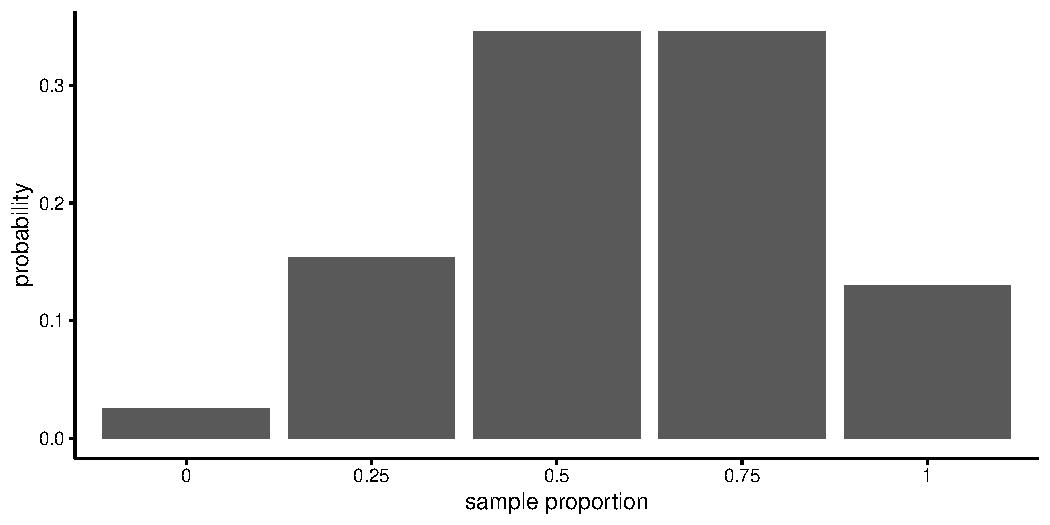
\includegraphics[width=\maxwidth]{figure/sampling_proportion-1} \caption[Sampling distribution of the sample proportion, when the population proportion is 0.60]{Sampling distribution of the sample proportion, when the population proportion is 0.60}\label{fig:sampling_proportion}
\end{figure}


\end{knitrout}



The proportion of tall elephants in the population is $p = 0.6$. The sample size equals $n = 4$. Let's begin with randomly picking the first elephant: what's the probability that we select an elephant that is taller than 3.40 m? Well, that probability is equal to the proportion of 0.6. Next, what is the probability that the second elephant is taller than 3.40? Again, this is equal to 0.6. 

Now something more complicated: what is the probability that both the first \textit{and} the second elephant are taller than 3.40? This is equal to $0.6 \times 0.6 = 0.36$. What is the probability that \textit{all} 4 elephants are taller than 3.40 m? That is equal to $0.6 \times 0.6 \times 0.6 \times 0.6 = 0.60^4 = 0.1296$. The probability that all 4 elephants are shorter than 3.40 m is equal to $(1-0.6)^4 = 0.4^4=0.0256$. 

The probability for a mix of 2 tall elephants and 2 shorter elephants is more difficult to compute. You might remember from high school that it involves \textit{combinations}. For example, the probability that the first 2 elephants are taller than 3.40, and the last 2 elephants shorter, is equal to $0.6^2 \times (1-0.6)^2 = 0.0576$, but there are many other ways in which we can find 2 tall elephants and 2 shorter elephants when we randomly and sequentially pick 4 elephants. There are in fact 6 different ways of randomly selecting 4 elephants where only 2 are tall. When we use A to denote a tall elephant and B to denote a short elephant, the 6 possible combinations of having two As and two Bs are in fact: AABB, BBAA, ABAB, BABA, ABBA, and BAAB. 

This number of combinations is calculated using the \textit{binomial coefficient}:

\begin{equation}
 {4\choose 2} = \frac{4!}{2!2!} = 6
\end{equation}

This number ${4\choose 2}$ ('four choose two') is called the binomial coefficient. It can be calculated using \textit{factorials}: the exclamation mark $!$ stands for factorial. For instance, $5!$ ('five factorial') means $5\times 4 \times 3 \times 2 \times 1$. 


In its general form, the binomial coefficient looks like:

\begin{equation}
 {n\choose r} = \frac{n!}{r!(n-r)!} 
\end{equation}

So suppose sample size $n$ is equal to 4 and $r$ equal to 2 (the number of tall elephants in the sample), we get:

\begin{equation}
{4\choose 2} = \frac{4!}{2!(n-r)!} = \frac{4!}{2!2!} =
\frac{4\times 3 \times 2 \times 1}{2 \times 1 \times  2 \times 1} = 6
\end{equation} 

Going back to the elephant example, there are ${4\choose 2}=6$ possible ways of getting 2 tall elephants and 2 short elephants when we sequentially pick 4 elephants. Each of these possibilities has a probability of $0.6^2 \times (1-0.6)^2 = 0.0576$. This is explained in Table \ref{tab:permutations}. For instance, the probability of getting the ordering ABAB, is equal to the multiplication of the respective probabilities: $0.6 \times 0.4 \times 0.6 \times 0.4$. In the table you can see that the probability for any ordering is always 0.0576. Since any ordering will qualify as obtaining 2 tall elephants from a total of 4, we can sum these probabilities: the probability of getting the ordering AABB \textit{or} BBAA \textit{or} ABAB \textit{or} BABA \textit{or} ABBA \textit{or} BAAB, is equal to $0.0576 + 0.0576 + 0.0576 + 0.0576 + 0.0576 + 0.0576 = 6 \times 0.0576 = 0.3456 $. Here 6 is the number of combinations, calculated as the binomial coefficient ${4\choose 2}$. We could therefore in general compute the probability of having 2 tall elephants in a sample of 4 as

\begin{equation}
 p(\#A = 2 | n = 4, p = 0.6) = {4\choose 2} \times 0.6^2 \times (1-0.6)^2 = 6 \times 0.0576 =
 0.3456
\end{equation}


The probability of ending up with 2 tall elephants in a sample of 4 elephants, in any order, and where the proportion of tall elephants in the population is 0.6, is therefore equal to 0.3456. 


In the more general case, if you have a population with a proportion $p$ of As, a sample size of $n$, and you want to know the probability of finding $r$ instances of A in your sample, it can be computed with the formula


\begin{equation}
 p(\#A = r | n, p) = {n\choose r} \times p^r \times (1-p)^{(n-r)} 
\end{equation}

For example, the probability of obtaining 3 tall elephants when the total number of elephants is 4, is ${4\choose 3} \times 0.6^3 \times (1-0.6)^{1}  = 4 \times 0.216  \times 0.4  = 0.3456 $.

When we calculate the probabilities of finding 0, 1, 2, 3, or 4 tall elephants in sample of 4 when the population proportion is 0.6, we obtain the \textit{binomial distribution} that is plotted in Figure \ref{fig:binomial}. It is exactly the same as the sampling distribution in Figure \ref{fig:sampling_proportion}, except that we plot the number of tall elephants in the sample on the horizontal axis, instead of the proportion. This means that we can use the binomial distribution to describe the sampling distribution of the sample proportion. To get the proportions, we simply divide the number of tall elephants in our sample by the total number of elephants ($n$) and we get Figure \ref{fig:sampling_proportion}. 






% latex table generated in R 4.0.3 by xtable 1.8-4 package
% Sun Jan 31 16:37:18 2021
\begin{table}[ht]
\centering
\caption{Four possible ways of selecting 2 tall elephants (A) and 2 short elephants (B), together with the probability for each selection.} 
\label{tab:permutations}
\begin{tabular}{llr}
  \hline
ordering & computation of probability & probability \\ 
  \hline
AABB & 0.6 x 0.6 x 0.4 x 0.4 & 0.0576 \\ 
  ABAB & 0.6 x 0.4 x 0.6 x 0.4 & 0.0576 \\ 
  ABBA & 0.6 x 0.4 x 0.4 x 0.6 & 0.0576 \\ 
  BAAB & 0.4 x 0.6 x 0.6 x 0.4 & 0.0576 \\ 
  BABA & 0.4 x 0.6 x 0.4 x 0.6 & 0.0576 \\ 
  BBAA & 0.4 x 0.4 x 0.6 x 0.6 & 0.0576 \\ 
   \hline
\end{tabular}
\end{table}



\begin{knitrout}
\definecolor{shadecolor}{rgb}{0.969, 0.969, 0.969}\color{fgcolor}\begin{figure}
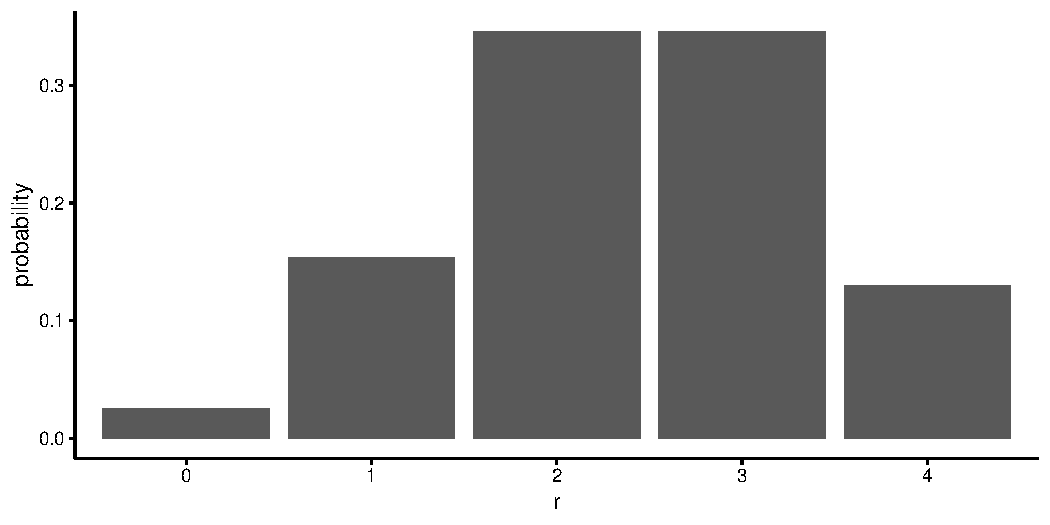
\includegraphics[width=\maxwidth]{figure/binomial-1} \caption[Binomial distribution with $n=4$ and $p=0.60$]{Binomial distribution with $n=4$ and $p=0.60$.}\label{fig:binomial}
\end{figure}


\end{knitrout}


\bigskip



\noindent\fbox{%
    \parbox{\textwidth}{%
\textbf{Overview}
\begin{itemize}

\item \textbf{sampling distribution of the sample proportion}: the distribution of proportions that you get when you randomly pick new samples from a population and for each sample compute the proportion.

\item \textbf{binomial distribution}: a discrete distribution showing the probabilities of finding a certain number of successes ($r$), given sample size $n$ and population proportion $p$.

\item \textbf{binominal coefficient}: a coefficient used to calculate binomial probabilities. It represents the number of ways in which you can find $r$ instances in a sample of size $n$. It is calculated as ${n\choose r} = \frac{n!}{r!(n-r)!}$.

\end{itemize}

}%
}


\bigskip



\section{Confidence intervals}

Based on what we know about the binomial distribution, we can perform inference on proportions. In Chapter \ref{chap:mean} we saw that inference is very much based on the standard error (i.e., the standard deviation of the sampling distribution). We know from theory that the variance of the binomial distribution can be easily calculated as $n \times p \times (1-p)$. Because we want to have the variance in proportions rather than in numbers, we have to divide this variance by $n$ to get the variance of proportions: $\frac{n \times p \times (1-p)}{n} = p \times (1-p) $. Next, because the variance of a sampling distribution gets smaller with increasing $n$, we divide by $n$ again, in a similar way as we did for the sampling distribution of the sample mean in Chapter \ref{chap:mean}. Taking the square root of this variance gives us the standard deviation of the sampling distribution (i.e., the standard error):


\begin{equation}
\sigma_{\hat{p}} = \sqrt{\frac{p(1-p)}{n}}
\end{equation}

This standard error makes it easy to construct confidence intervals. We know from the Central Limit Theorem that if $n$ becomes infinitely large, the sampling distribution will become normal. When $n=50$, the sampling distribution is already close to normal, as is shown in Figure \ref{fig:sampling_50}. This fact, together with the standard error makes it easy to construct approximate confidence intervals.


Suppose that we had 50 elephants in our zoo, and the manager observed that 42 of them bump their head against the doorway. That is a sample proportion of $\frac{42}{50}= 0.84$. When we want to have a range of plausible values for the population proportion, we can construct a 95\% confidence interval around this sample proportion. Because we know that for the standard normal distribution, 95\% of the observations are between -1.96 and +1.96, we construct the 95\% confidence interval by multiplying 1.96 with the standard error, $\sigma_{\hat{p}} = \sqrt{\frac{p(1-p)}{n}}$.


However, since we do not know the population proportion $p$, we have to estimate it. From theory, we know that an unbiased estimator for the population proportion is the sample proportion: $\hat{p} = \frac{42}{50}= 0.84$. Our estimate for the standard error is then $\sqrt{\frac{\hat{p}(1-\hat{p})}{n}} = 0.0518459$.

If we use that value, we get the interval from $0.84 - 1.96 \times 0.0518459$ to $0.84 + 1.96 \times 0.0518459$: thus, our 95\% confidence interval for the population proportion runs from 0.738382 to 0.941618.



\begin{knitrout}
\definecolor{shadecolor}{rgb}{0.969, 0.969, 0.969}\color{fgcolor}\begin{figure}
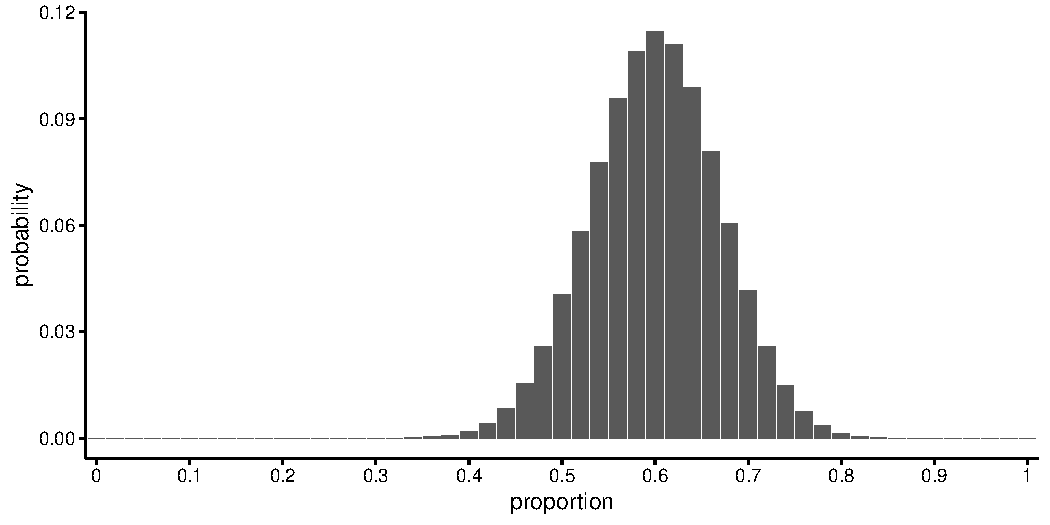
\includegraphics[width=\maxwidth]{figure/sampling_50-1} \caption[Sampling distribution with $n=50$ and $p=0.60$]{Sampling distribution with $n=50$ and $p=0.60$.}\label{fig:sampling_50}
\end{figure}


\end{knitrout}


\section{Null-hypothesis concerning a proportion}

Suppose that a researcher has measured all Tanzanian elephants and noted that a proportion of 0.60 was taller than 3.40 m. Suppose also that the manager in the zoo finds that 42 out of the 50 elephants bump their head and are therefore taller than 3.40. How can we know that the elephants could be a representative sample of Tanzanian elephants? 

To answer this question with a yes or a no, we could apply the logic of null-hypothesis testing. Let the null-hypothesis be that the population proportion is equal to 0.60, and the alternative hypothesis that it is not equal to 0.60. 

\begin{eqnarray}
H_0: p = 0.60 \\
H_A: p \neq 0.60
\end{eqnarray}

Is the proportion of 0.84 that we observe in the sample (the zoo) a probable value to find if the proportion of all Tanzanian is equal to 0.60? If this is the case, we do not reject the null-hypothesis, and believe that the zoo data could have been randomly selected from the Tanzanian population and are therefore representative. However, if the proportion of 0.84 is very unprobable given that the population proportion is 0.60, we reject the null-hypothesis and believe that the data are not representative.

With null-hypothesis testing we always have to fix our $\alpha$ first: the probability with which we are willing to accept a type I error. We feel it is really important that the sample is representative of the population, so we definitely do not want to make the mistake that we think the sample is representative (not rejecting the null-hypothesis) while it isn't ($H_A$ is true). This would be a type II error (check this for yourself!). If we want to minimise the probability of a type II error ($\beta$), we have to pick a relatively high $\alpha$ (see Chapter \ref{chap:mean}), so let's choose our $\alpha = .10$. 

Next, we have to choose a test statistic and determine critical values for it that go with an $\alpha$ of .10. Because we have a relatively large sample size of 50, we assume that the sampling distribution for a proportion of 0.60 is normal. From the standard normal distribution, we know that 90\% ($1-\alpha$!) of the values lie between $-1.6448536$ and $1.6448536$ (see Table \ref{tab:t_table2}). If we therefore standardise our proportion, we have a measure that should show a standard normal distribution:

\begin{equation}
z_p = \frac{p_s - p_0}{sd} 
\end{equation}

where $z_p$ is the $z$-score for a proportion, $p_s$ is the sample proportion, $p_0$ is the population proportion assuming $H_0$, and $sd$ is the standard deviation of the sampling distribution, which is the standard error. Note that we should take the standard error that we get when the null-hypothesis is true. We then get

\begin{equation}
z_p = \frac{0.84 - 0.6}{se} = \frac{0.24}{\sqrt{\frac{p_0(1-p_0)}{n}}} = \frac{0.24}{0.069282} = 3.4641016
\end{equation}


90\% of the values in any normal distribution lie between $\pm 1.64$ standard deviations away from the mean (see Table \ref{tab:t_table2}). Here we see a $z$-score that exceeds these critical values, and we therefore reject the null-hypothesis. We conclude that the proportion of tall elephants observed in the sample is larger than to be expected under the assumption that the population proportion is 0.6. We decide that the zoo data are not representative of the population data. 

The decision process is illustrated in Figure \ref{fig:z-test}.

\begin{knitrout}
\definecolor{shadecolor}{rgb}{0.969, 0.969, 0.969}\color{fgcolor}\begin{figure}

{\centering 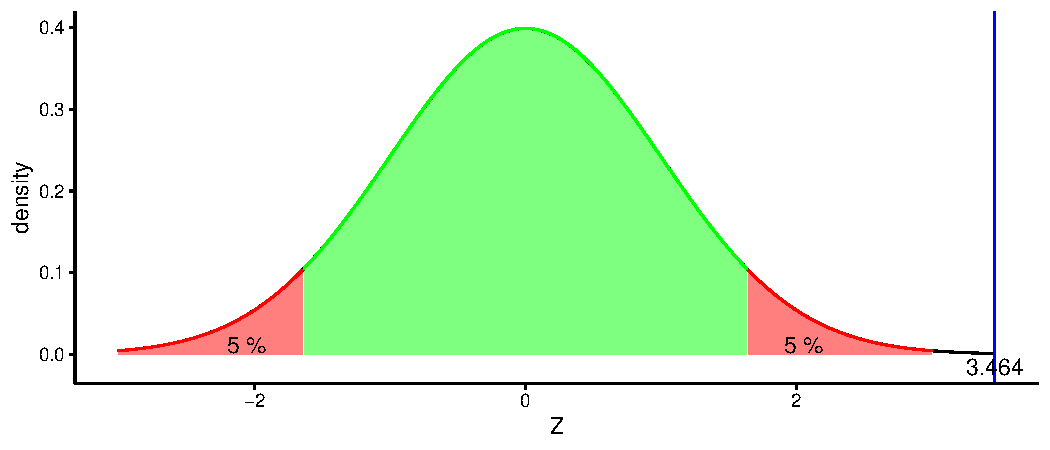
\includegraphics[width=\maxwidth]{figure/z-test-1} 

}

\caption[A normal distribution to test the null-hypothesis that the population proportion is 0.6]{A normal distribution to test the null-hypothesis that the population proportion is 0.6. The blue line represents the $z$-score for our observed sample proportion of 0.84.}\label{fig:z-test}
\end{figure}


\end{knitrout}


\section{Inference on proportions using R}

Using the normal distribution is a nice trick when you have to do the calculations by hand. However, this approach is of course only valid when you have large sample sizes, so that you know that the shape of the normal distribution is a good approximation of the binomial distribution. In contrast, using the binomial distribution always gives you the most exact answers. However it can be very tiresome to do all the computations by hand. In this section we discuss how to let R do the calculations for you.

Suppose we have a sample of 50 elephants, and we see that 42 of them bump their head against the doorway. What can we say about the population: what proportion of elephants in the entire population will bump their heads? In R, we use the \texttt{binom.test()} function to do inference on proportions. This function does all the calculations using the binomial distribution, so that the results are always trustworthy, even for small sample sizes. We state the number of observed elephants that bump their head (\texttt{x = 42}), the sample size (\texttt{n = 50}), the kind of confidence interval (95\%: \texttt{conf.level = 0.95}) and the proportion that we want to use for the null-hypothesis (\texttt{p = 0.6}):

\begin{knitrout}
\definecolor{shadecolor}{rgb}{0.969, 0.969, 0.969}\color{fgcolor}\begin{kframe}
\begin{alltt}
\hlkwd{binom.test}\hlstd{(}\hlkwc{x} \hlstd{=} \hlnum{42}\hlstd{,} \hlkwc{n} \hlstd{=} \hlnum{50}\hlstd{,} \hlkwc{conf.level} \hlstd{=} \hlnum{0.95}\hlstd{,} \hlkwc{p} \hlstd{=} \hlnum{0.6}\hlstd{)}
\end{alltt}
\begin{verbatim}
## 
## 	Exact binomial test
## 
## data:  42 and 50
## number of successes = 42, number of trials = 50, p-value = 0.0004116
## alternative hypothesis: true probability of success is not equal to 0.6
## 95 percent confidence interval:
##  0.7088737 0.9282992
## sample estimates:
## probability of success 
##                   0.84
\end{verbatim}
\end{kframe}
\end{knitrout}

The output shows the sample proportion: the probability of success is 0.84. This is of course $\frac{42}{50}$. If we want to know what the population proportion is, we look at the 95\% confidence interval that runs from 0.7088737 to 0.9282992. If you want to test the null-hypothesis that the population proportion is equal to 0.60, then we see that the $p$-value for that test is .0004116.

\begin{quotation}
"With a binomial test, we tested the null-hypothesis that the population proportion of elephants taller than 3.40 m is equal to 0.60. Our sample proportion, based on 50 elephants, was 0.84, which is significantly different from 0.6, $p < .001$. We therefore reject the null-hypothesis."
\end{quotation}


As said, the binomial test also works fine for small sample sizes. Let's go back to the very first example of this chapter: the zoo manager sees that of the 4 elephants they have, 3 bump their head and are therefore taller than 3.40 m. What does that tell us about the proportion of elephants worldwide that are taller than 3.40 m? If we assume that the 4 zoo elephants were randomly selected from the entire population of elephants, we can use the binomial distribution. In this case we type in R:

\begin{knitrout}
\definecolor{shadecolor}{rgb}{0.969, 0.969, 0.969}\color{fgcolor}\begin{kframe}
\begin{alltt}
\hlkwd{binom.test}\hlstd{(}\hlkwc{x} \hlstd{=} \hlnum{3}\hlstd{,} \hlkwc{n} \hlstd{=} \hlnum{4}\hlstd{)}
\end{alltt}
\begin{verbatim}
## 
## 	Exact binomial test
## 
## data:  3 and 4
## number of successes = 3, number of trials = 4, p-value = 0.625
## alternative hypothesis: true probability of success is not equal to 0.5
## 95 percent confidence interval:
##  0.1941204 0.9936905
## sample estimates:
## probability of success 
##                   0.75
\end{verbatim}
\end{kframe}
\end{knitrout}

By default, \texttt{binom.test()} yields 95\% confidence intervals, as can be seen in the output.\footnote{Note in the output that by default, \texttt{binom.test()} chooses the null-hypothesis that the population proportion is 0.5.} We see that the confidence interval for the population proportion runs from 0.1941204 to 0.9936905. Thus, based on this sample proportion of 0.75, we can see with some degree of confidence that the population proportion is somewhere between 0.19 and 0.99. That's of course not very informative, which makes sense considering we only observe 4 elephants.

We could report:


\begin{quotation}
"In our sample of 4 elephants, 3 were taller than 3.40 m. The 95\% confidence interval for the proportion of elephants in the population that are taller than 3.40 m runs from 0.19 to 0.99."
\end{quotation}

or, somewhat shorter:

\begin{quotation}
"Based on a sample of 4 elephants, our estimate for the proportion of elephants in the population that are taller than 3.40 m is 0.75 (95\% CI: 0.19, 0.99)."
\end{quotation}

   % label prop


\chapter{Linear modelling: introduction}\label{chap:simple}



% 110.	Linear equations (and models) 
% •	Students are able to identify dependent and independent variables in a causal or predictive statement implied in a research hypothesis.
% •	Students are able to interpret both negative and positive constants (intercepts) and both negative and positive regression slope coefficients for numeric variables.  
% •	Students are able to interpret both negative and positive constants (intercepts) and both negative and positive regression slope coefficients for numeric variables in a visual/graphical way.


\section{Dependent and independent variables}

In the previous two chapters we discussed single variables. In Chapter \ref{chap:mean} we discussed a numeric variable that had a certain mean, for instance we talked about the height of elephants. In Chapter \ref{chap:prop} we talked about a dichotomous categorical variable: elephants being taller than 3.40 m or not, with a certain proportion of tall elephants. This chapter deals with the relationship between two variables, more specifically the relationship between two numeric variables. 

In Chapter \ref{chap:intro} we discussed the distinction between numeric, ordinal and categorical variables. In linear modelling, there is also another important distinction between variables: \textit{dependent} and \textit{independent} variables. Dependency of a variable is not really a property of a variable but it is the result of the data analyst's choice. Let's first think about relationships between two variables. Determining whether a variable is to be treated as independent or not, is often either a case of logic or a case of theory. When studying the relationship between the height of a mother and that of her child, the more logical it would be to see the height of the child \textit{as dependent} on the height of the mother. This is because we assume that the genes are transferred from the mother to the child. The mother comes first, and the height of the child is partly the \textit{result} of the mother's genes that were transmitted during fertilisation. The height of a child depends in part on the height of the mother. The variable that measures the result is usually taken as the \textit{dependent} variable. The theoretical cause or antecedent is usually taken as the \textit{independent} variable. 

The dependent variable is often called the \textit{response variable}. An independent variable is often called a \textit{predictor variable} or simply \textit{predictor}. Independent variables are also often called \textit{explanatory} variables. We can explain a very tall child by the genes that it got from its very tall mother. The height of a child is then the response variable, and the height of the mother is the explanatory variable. We can also predict the adult height of a child from the height of the mother.

The dependent variable is usually the most central variable. It is the variable that we'd like to understand better, or perhaps predict. The independent variable is usually an explanatory variable: it explains why some people have high values for the dependent variable and other people have low values. For instance, we'd like to know why some people are healthier than others. Health may then be our dependent variable. An explanatory variable might be age (older people tend to be less healthy), or perhaps occupation (being a dive instructor induces more health problems than being a university professor). 

Sometimes we're interested to see whether we can predict a variable. For example, we might want to predict longevity. Age at death would then be our dependent variable and our independent (predictor) variables might concern lifestyle and genetic make-up. 

Thus, we often see four types of relations:
\begin{itemize}
\item Variable $A$ affects/influences another variable $B$.
\item Variable $A$ causes variable $B$.
\item Variable $A$ explains variable $B$.
\item Variable $A$ predicts variable $B$.
\end{itemize}

In all these four cases, variable $A$ is the independent variable and variable $B$ is the dependent variable.

Note that in general, dependent variables can be either numeric, ordinal, or categorical. Also independent variables can be numeric, ordinal, or categorical. 

% \subsection{Exercises}
% 
% Below, variables are printed in \textbf{bold}. For each research statement, identify which variable is the dependent variable, and which variable is the independent variable.
% 
% \begin{enumerate}
% 
% \item The effect of \textbf{income} on \textbf{health}
% \item \textbf{Stock value} is affected by \textbf{inflation}
% \item \textbf{Size} is influenced by \textbf{weight}
% \item \textbf{Shoe size} is predicted by \textbf{sex}
% \item The less you \textbf{drink} the more \textbf{thirsty} you become 
% \item The more \textbf{calories} you eat, the more you \textbf{weigh}
% \item \textbf{Weight} is affected by \textbf{food intake} 
% \item \textbf{Weight} is affected by \textbf{exercise} 
% \item \textbf{Food intake} is predicted by \textbf{time of year}
% \item There is an effect of \textbf{exercise} on \textbf{heart rate} 
% \item \textbf{Inflation} leads to higher \textbf{wages} 
% \item \textbf{Unprotected sex} leads to \textbf{pregnancy}
% \item \textbf{HIV-infection} is caused by \textbf{unprotected sex}
% \item The effect of \textbf{alcohol intake} on \textbf{driving performance}
% \item \textbf{Sunshine} causes \textbf{growth}
% 
% 
% \end{enumerate}
% 
% Answers:
% 
% \begin{enumerate}
% 
% \item \textbf{income} independent, \textbf{health} dependent.
% \item \textbf{Stock value} dependent, \textbf{inflation} independent
% \item \textbf{Size} dependent, \textbf{weight} independent
% \item \textbf{Shoe size} dependent, \textbf{sex} independent
% \item \textbf{drink} independent, \textbf{thirsty} dependent
% \item \textbf{calories} independent, \textbf{weigh} dependent
% \item \textbf{Weight} dependent, \textbf{food intake} independent
% \item \textbf{Weight} dependent, \textbf{exercise} independent
% \item \textbf{Food intake} dependent, \textbf{time of year} independent
% \item \textbf{exercise} independent, \textbf{heart rate} dependent
% \item \textbf{Inflation} independent, \textbf{wages} dependent
% \item \textbf{Unprotected sex} independent, \textbf{pregnancy} dependent
% \item \textbf{HIV-infection} dependent, \textbf{unprotected sex} independent
% \item \textbf{alcohol intake} independent, \textbf{driving performance} dependent
% \item \textbf{Sunshine} independent, \textbf{growth} dependent
% 
% 
% \end{enumerate}



\section{Linear equations}\label{sec:equations}


\begin{knitrout}
\definecolor{shadecolor}{rgb}{0.969, 0.969, 0.969}\color{fgcolor}\begin{figure}

{\centering 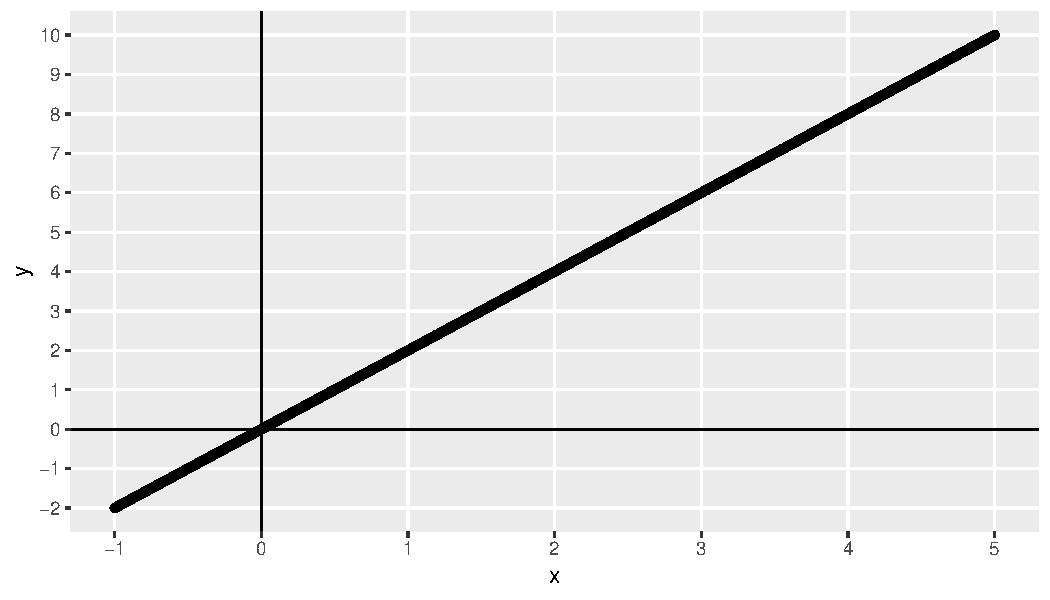
\includegraphics[width=\maxwidth]{figure/lm_1-1} 

}

\caption[Straight line with intercept 0 and slope 2]{Straight line with intercept 0 and slope 2.}\label{fig:lm_1}
\end{figure}


\end{knitrout}


From secondary education you might remember linear equations. Suppose you have two quantities, $X$ and $Y$, and there is a straight line that describes best their relationship. An example is given in Figure \ref{fig:lm_1}. We see that for every value of $X$, there is only one value of $Y$. Moreover, the larger the value of $X$, the larger the value of $Y$. If we look more closely, we see that for each increase of 1 unit in $X$, there is an increase of 2 units in $Y$. For instance, if $X=1$, we see a $Y$-value of 2, and if $X=2$ we see a $Y$-value of 4. So if we move from $X=1$ to $X=2$ (a step of one on the $X$-axis), we move from 2 to 4 on the $Y$-axis, which is an increase of 2 units. This increase of 2 units for every step of 1 unit in $X$ is the same for all values of $X$ and $Y$. For instance, if we move from 2 to 3 on the $X$-axis, we go from 4 to 6 on the $Y$-axis: an increase of again 2 units. This constant increase is typical for linear relationships. The increase in $Y$ for every unit increase in $X$ is called the \textit{slope} of a straight line. In this figure, the slope is equal to 2.

The slope is one important characteristic of a straight line. The second important property of a straight line is the \textit{intercept}. The intercept is the value of $Y$, when $X=0$. In Figure \ref{fig:lm_1} we see that when $X=0$, $Y$ is 0, too. Therefore the intercept of this straight line is 0.

With the intercept and the slope, we completely describe this straight line: no other information is necessary. Such a straight line describes a \textit{linear relationship} between $X$ and $Y$. The linear relationship can be formalised using a linear equation. The general form of a linear equation for two variables $X$ and $Y$ is the following:

\begin{equation}
Y = \textrm{intercept} + \textrm{slope} \times X
\end{equation}


For the linear relationship between $X$ and $Y$ in Figure \ref{fig:lm_1} the linear equation is therefore

\begin{equation}
Y = 0 + 2 X
\end{equation}

which can be simplified to

\begin{equation}
Y =  2 X
\end{equation}


With this equation, we can find the $Y$-value for all values of $X$. For instance, if we want to know the $Y$-value for $X=3.14$, then using the linear equation we know that $Y = 2 \times 3.14 = 6.28$. If we want to know the $Y$-value for $X=49876.6$, we use the equation to obtain $Y=2\times 49876.6 = 99753.2$. In short, the linear equation is very helpful to quickly say what the $Y$-value is on the basis of the $X$-value, even if we don't have a graph of the relationship or if the graph does not extent to certain $X$-values.


In the linear equation, we call $Y$ the \textit{dependent} variable, and $X$ the \textit{independent} variable. This is because the equation helps us determine or predict our value of $Y$ on the basis of what we know about the value of $X$. When we graph the line that the equation represents, such as in Figure \ref{fig:lm_1}, the common way is to put the dependent variable on the vertical axis, and the independent variable on the horizontal axis. 


Figure \ref{fig:lm_2} shows a different linear relationship between $X$ and $Y$. First we look at the slope: we see that for every unit increase in $X$ (from 1 to 2, or from 4 to 5) we see an increase of 0.5 in $Y$. Therefore the slope is equal to 0.5. Second, we look at the intercept: we see that when $X=0$, $Y$ has the value -2. So the intercept is -2. Again, we can describe the linear relationship by a linear equation, which is now:

\begin{equation}
Y = -2 + 0.5 X
\end{equation}



\begin{knitrout}
\definecolor{shadecolor}{rgb}{0.969, 0.969, 0.969}\color{fgcolor}\begin{figure}

{\centering 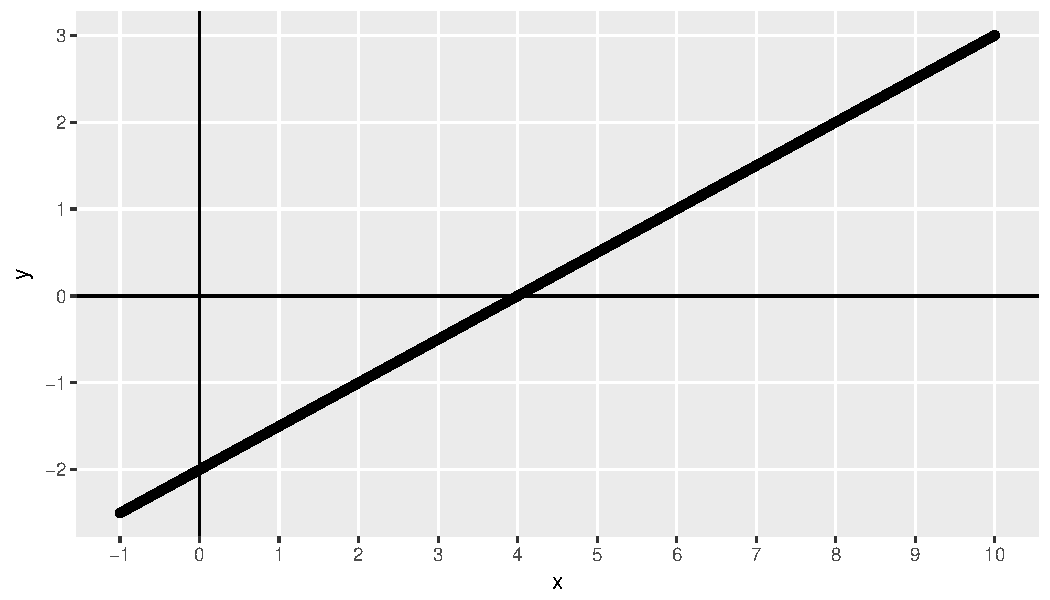
\includegraphics[width=\maxwidth]{figure/lm_2-1} 

}

\caption[Straight line with intercept -2 and slope 0.5]{Straight line with intercept -2 and slope 0.5.}\label{fig:lm_2}
\end{figure}


\end{knitrout}


Linear relationships can also be negative, see Figure \ref{fig:lm_3}. There, we see that if we move from 0 to 1, we see a \textit{decrease} of 2 in $Y$ (we move from $Y = -2$ to $Y = -4$), so $-2$ is our slope value. Because the slope is negative, we call the relationship between the two variables negative. Further, when $X=0$, we see a $Y$-value of -2, and that is our intercept. The linear equation is therefore:

\begin{equation}
Y = -2 - 2 X
\end{equation}


\begin{knitrout}
\definecolor{shadecolor}{rgb}{0.969, 0.969, 0.969}\color{fgcolor}\begin{figure}

{\centering 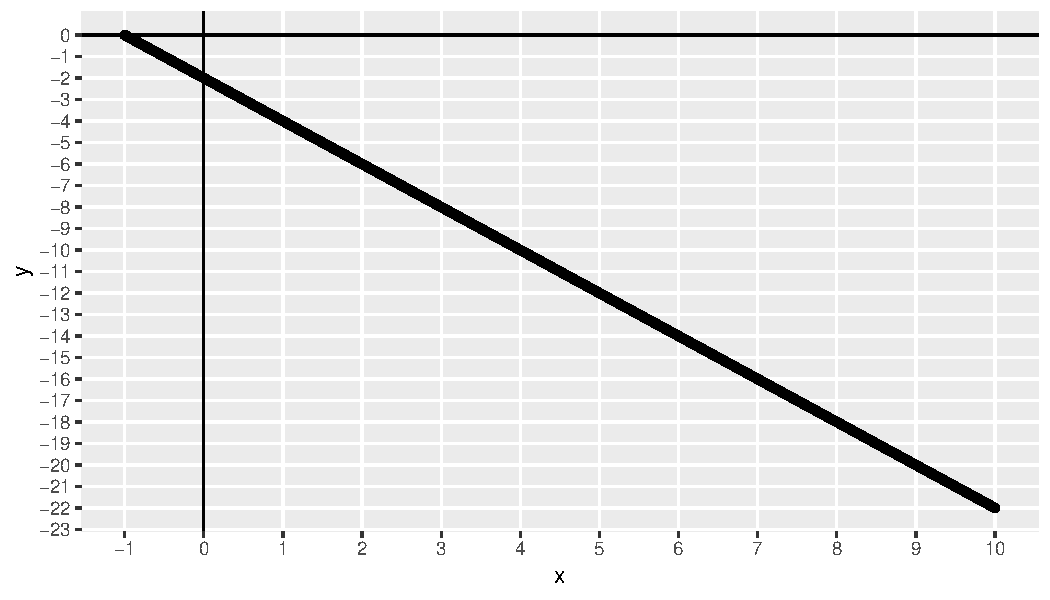
\includegraphics[width=\maxwidth]{figure/lm_3-1} 

}

\caption[Straight line with intercept -2 and slope -2]{Straight line with intercept -2 and slope -2.}\label{fig:lm_3}
\end{figure}


\end{knitrout}



\bigskip



\noindent\fbox{%
    \parbox{\textwidth}{%
\textbf{Overview}
\begin{itemize}

\item \textbf{dependent variable}: the variable that we want to describe, understand, predict or explain. Usually denoted as $Y$.

\item \textbf{independent variable}: the variable that we use in order to understand, predict or explain something. Usually denoted as $X$. 

\item \textbf{linear relationship}: two variables are said to be linearly related if their relationship can be described by a linear equation with an intercept and a slope.

\item \textbf{intercept}: the value for $Y$ (dependent variable) if $X=0$ (independent variable).

\item \textbf{slope}: the change in $Y$ when we increase $X$ by 1 unit.



\end{itemize}

}%
}


\bigskip



% \subsection{Exercises}
% 
% \begin{enumerate}
% \item
% For Figures \ref{fig:lm_4}, \ref{fig:lm_5} and \ref{fig:lm_6}, give the linear equations for the relationship between $x$ and $y$.
% 
% 
% <<lm_4,fig.height=4, echo=FALSE, fig.align='center', fig.cap='Straight line example.'>>=
% x = seq(-1,10,0.01)
% y = 3 - 1*x
% tibble(x, y) %>% ggplot(aes(x,y)) + geom_point()+
%         geom_vline(xintercept=0)+ geom_hline(yintercept = 0) + scale_x_continuous(breaks=seq(-1,10,1), minor_breaks =seq(-1,10,1) ) +
% scale_y_continuous(breaks=seq(-60,20,1), minor_breaks =seq(-60,20,1))
% @
% 
% <<lm_5,fig.height=4, echo=FALSE, fig.align='center', fig.cap='Straight line example.'>>=
% x = seq(-1,10,0.01)
% y = 1.5 - 0.5*x
% tibble(x, y) %>% ggplot(aes(x,y)) + geom_point()+
%         geom_vline(xintercept=0)+ geom_hline(yintercept = 0) + scale_x_continuous(breaks=seq(-1,10,1), minor_breaks =seq(-1,10,1) ) +
% scale_y_continuous(breaks=seq(-60,20,1), minor_breaks =seq(-60,20,1))
% @
% 
% <<lm_6,fig.height=4, echo=FALSE, fig.align='center', fig.cap='Straight line example.'>>=
% x = seq(-1,10,0.01)
% y = -1.5 + 0.3333333333*x
% tibble(x, y) %>% ggplot(aes(x,y)) + geom_point()+
%         geom_vline(xintercept=0)+ geom_hline(yintercept = 0) + scale_x_continuous(breaks=seq(-1,10,1), minor_breaks =seq(-1,10,1) ) +
% scale_y_continuous(breaks=seq(-60,20,1), minor_breaks =seq(-60,20,1))
% @
% \item
% Try to sketch the straight line for the equation $y=1 - 2x$
% 
% 
% \end{enumerate}
% 
% 
% \subsection{Answers}
% 
% The equations are
% \begin{enumerate}
% \item 
% \begin{equation}
% y = 3 - 1 x
% \end{equation}
% \item
% \begin{equation}
% y = 1.5 - 0.5 x
% \end{equation}
% \item
% \begin{equation}
% y = -2 + 0.33 x
% \end{equation}
% \item
% The straight line for $y=1 - 2x$ is presented in Figure \ref{fig:lm_7}.
% 
% <<lm_7,fig.height=4, echo=FALSE, fig.align='center', fig.cap='Straight line with based on y=1-2x.'>>=
% x = seq(-1,5,0.01)
% y = 1 -2*x
% tibble(x, y) %>% ggplot(aes(x,y)) + geom_point()+
%         geom_vline(xintercept=0)+ geom_hline(yintercept = 0) + scale_x_continuous(breaks=seq(-1,5,1), minor_breaks =seq(-1,5,1) ) +
% scale_y_continuous(breaks=seq(-10,20,1), minor_breaks =seq(-10,20,1))
% @
% \end{enumerate}

\section{Linear regression}

In the previous section, we saw perfect linear relationships between quantities $X$ and $Y$: for each $X$-value there was only one $Y$-value, and the values are all described by a straight line. Such relationships we hope to see in physics, but mostly see only in mathematics.

In social sciences we hardly ever see such perfectly linear relationships between quantities (variables). For instance, let us plot the relationship between yearly income and the amount of Euros spent on holidays. Yearly income is measured in thousands of Euros (k Euros), and money yearly spent on holidays is measured in Euros. Let us regard money spent on holidays as our dependent variable and yearly income as our independent variable (we assume money needs to be saved before it can be spent). We therefore plot yearly income on the $X$-axis (horizontal axis) and holiday spendings on the $Y$-axis (vertical axis). Let's imagine we find the data from 100 women between 30 and 40 years of age that are plotted in Figure \ref{fig:lm_8}.


\begin{knitrout}
\definecolor{shadecolor}{rgb}{0.969, 0.969, 0.969}\color{fgcolor}\begin{figure}

{\centering 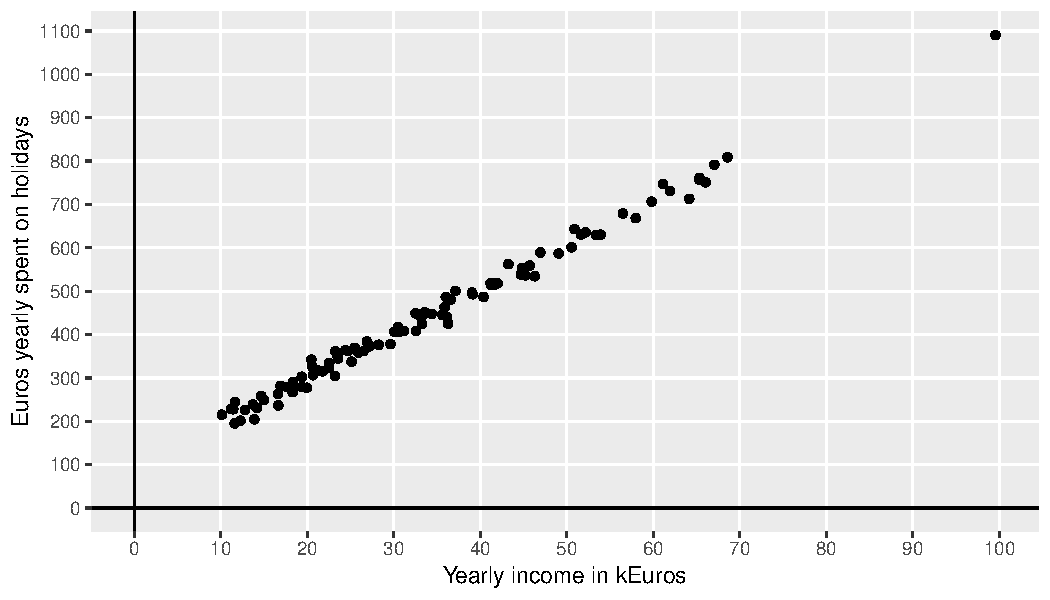
\includegraphics[width=\maxwidth]{figure/lm_8-1} 

}

\caption[Data on holiday spending]{Data on holiday spending.}\label{fig:lm_8}
\end{figure}


\end{knitrout}

In the scatter plot, we see that one woman has a yearly income of 100,000 Euros, and that she spends almost 1100 Euros per year on holidays. We also see a couple of women who earn less, between 10,000 and 20,000 Euros a year, and they spend between 200 and 300 Euros per year on holiday.

The data obviously do not form a straight line. However, we tend to think that the relationship between yearly income and holiday spending is more or less linear: there is a general linear trend such that for every increase of 10,000 Euros in yearly income, there is an increase of about 100 Euros.

Let's plot such a straight line that represents that general trend, with a slope of 100 straight through the data points. The result is seen in Figure \ref{fig:lm_9}. We see that the line with a slope of 100 is a nice approximation of the relationship between yearly income and holiday spendings. We also see that the intercept of the line is 100.

\begin{knitrout}
\definecolor{shadecolor}{rgb}{0.969, 0.969, 0.969}\color{fgcolor}\begin{figure}

{\centering 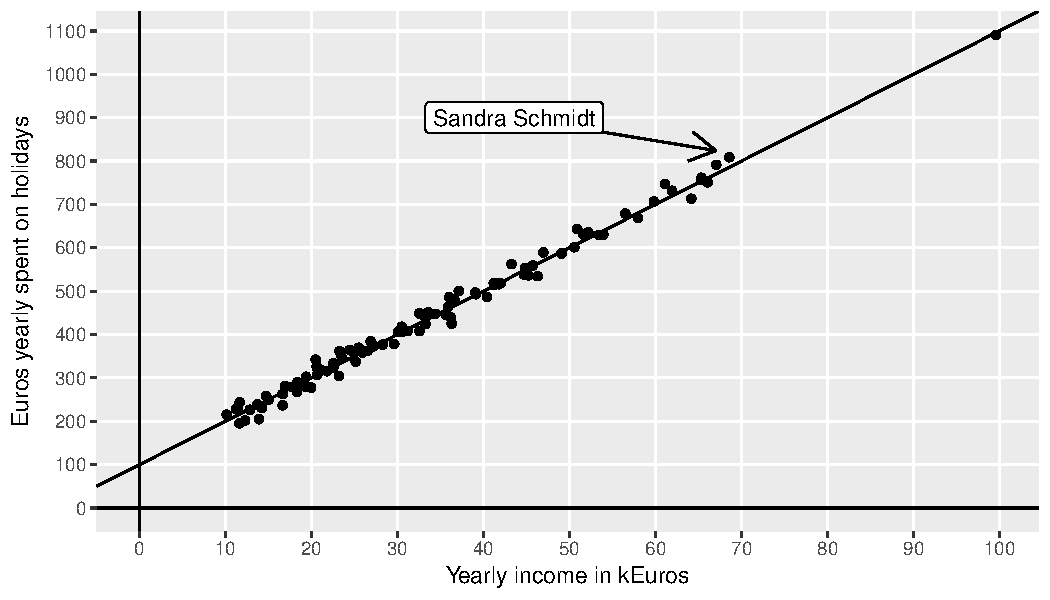
\includegraphics[width=\maxwidth]{figure/lm_9-1} 

}

\caption[Data on holiday spending with an added straight line]{Data on holiday spending with an added straight line.}\label{fig:lm_9}
\end{figure}


\end{knitrout}

Given the intercept and slope, the linear equation for the straight line approximating the relationship is

\begin{equation}
\texttt{HolidaySpendings} = 100 + 100 \times \texttt{YearlyIncome}
\end{equation}

In summary, data on two variables may not show a perfect linear relationship, but in many cases, a perfect straight line can be a very reasonable approximation of the data. Another word for a reasonable approximation of the data is a \textit{prediction model}. Finding such a straight line to approximate the data points is called \textit{linear regression}. In this chapter we will see what method we can use to find a straight line. In linear regression we describe the behaviour of the dependent variable (the $Y$-variable on the vertical axis) on the basis of the independent variable (the $X$-value on the horizontal axis) using a linear equation. We say that \textit{we regress variable $Y$ on variable $X$}.




\section{Residuals}

Even though a straight line can be a good approximation of a data set consisting of two variables, it is hardly ever perfect: there are always discrepancies between what the straight line describes and what the data actually tell us.

For instance, in Figure \ref{fig:lm_9}, we see a woman, Sandra Schmidt, who makes 69 k Euros a year and who spends 809 Euros on holidays. According to the linear equation that describes the straight line, a woman that earns 69 k Euros a year would spend $100 + 100 \times 69= 786$ Euros on holidays. The discrepancy between the actual amount spent and the amount prescribed by the linear equation equals $809-786=23$ Euros. This difference is rather small and the same holds for all the other women in this data set. Such discrepancies between the actual amount spent and the amount as prescribed or predicted by the straight line are called \textit{residuals} or \textit{errors}. The residual (or error) is the difference between a certain data point (the \textit{actual} value) and what the linear equation predicts.


% Using the linear equation, we could predict holiday spendings even for yearly incomes that are not in the data set. For instance, in this data set there is no woman with an income of 80,000, but still we can use the linear equation with a prediction that such a woman would probably spend around $100+100\times 80= 8100$ Euros.


Let us look at another fictitious data set where the residuals (errors) are a bit larger. Figure \ref{fig:lm_10} shows the relationship between variables $X$ and $Y$. The dots are the actual data points and the blue straight line is an approximation of the actual relationship. The residuals are also visualised: sometimes the observed $Y$-value is greater than the predicted $Y$-value (dots above the line) and sometimes the observed $Y$-value is smaller than the predicted $Y$-value (dots below the line). If we denote the $i$th predicted $Y$-value (predicted by the blue line) as $\widehat{Y_i}$ (pronounced as 'y-hat-i'), then we can define the residual or error as the discrepancy between the observed $Y_i$ and the predicted $\widehat{Y_i}$:

\begin{equation}
e_i = Y_i - \widehat{Y_i}
\end{equation}

where $e_i$ stands for the error (residual) for the $i$th data point .


\begin{knitrout}
\definecolor{shadecolor}{rgb}{0.969, 0.969, 0.969}\color{fgcolor}\begin{figure}

{\centering \includegraphics[width=\maxwidth]{figure/lm_10-1} 

}

\caption[Data on variables $X$ and $Y$ with an added straight line]{Data on variables $X$ and $Y$ with an added straight line.}\label{fig:lm_10}
\end{figure}


\end{knitrout}

If we compute residual $e_i$ for all $Y$-values in the data set, we can plot them using a histogram, as displayed in Figure \ref{fig:lm_11}. We see that the residuals are on average 0, and that the histogram resembles the shape of a normal distribution. We see that most of the residuals are around 0, and that means that most of the values $Y$-values are close to the line (where the predicted values are). We also see some large residuals but that there are not so many of these. Observing a more or less normal distribution of residuals happens often in research. Here, the residuals show a normal distribution with mean 0 and variance of 13336 (i.e., a standard deviation of 115).


\begin{knitrout}
\definecolor{shadecolor}{rgb}{0.969, 0.969, 0.969}\color{fgcolor}\begin{figure}

{\centering \includegraphics[width=\maxwidth]{figure/lm_11-1} 

}

\caption[Histogram of the residuals (errors)]{Histogram of the residuals (errors).}\label{fig:lm_11}
\end{figure}


\end{knitrout}


\section{Least squares regression lines}\label{sec:least_squares}


You may ask yourself how to draw a straight line through the data points: How do you decide on the exact slope and the exact intercept? And what if you don't want to draw the data points and the straight line by hand? That can be quite cumbersome if you have more than 2000 data points to plot!

First, because we are lazy, we always use a computer to draw the data points and the line, that we call a \textit{regression line}. Second, since we could draw many different straight lines through a scatter of points, we need a criterion to determine a nice combination of intercept and slope. With such a criterion we can then let the computer determine the regression line with its equation for us.

The criterion that we use in this chapter is called Least Squares, or Ordinary Least Squares (OLS). To explain the Least Squares principle, look again at Figure \ref{fig:lm_10} where we see both small and large residuals. About half of them are positive (above the blue line) and half of them are negative (below the blue line).

The most reasonable idea is to draw a straight line that is more or less in the middle of the $Y$-values, in other words, with about half of the residuals positive and about half of them negative. Or perhaps we could say that on average, the residuals should be 0. A third way of saying the same thing is that the sum of the residuals should be equal to 0.

However, the criterion that all residuals should sum to 0 is not sufficient. In Figure \ref{fig:lm_12} we see a straight line with a slope of 0 where the residuals sum to 0. However, this regression line does not make intuitive sense: it does not describe the structure in the data very well. Moreover, we see that the residuals are generally much larger than in Figure \ref{fig:lm_10}.

\begin{knitrout}
\definecolor{shadecolor}{rgb}{0.969, 0.969, 0.969}\color{fgcolor}\begin{figure}

{\centering \includegraphics[width=\maxwidth]{figure/lm_12-1} 

}

\caption[Data on variables $X$ and $Y$ with an added straight line]{Data on variables $X$ and $Y$ with an added straight line. The sum of the residuals equals 0.}\label{fig:lm_12}
\end{figure}


\end{knitrout}

We therefore need a second criterion to find a nice straight line. We want the residuals to sum to 0, but also want the residuals to be as small as possible: the discrepancies between what the linear equation predicts (the $\widehat{Y}$-values) and the actual $Y$-values should be as small as possible.

So now we have two criteria: we want the sum of the residuals to be 0 (about half of them negative, half of them positive), and we want the residuals to be as small as possible. We can achieve both of these when we use as our criterion the idea that the sum of the \textit{squared} residuals be as small as possible. Recall from Chapter \ref{chap:intro} that the sum of the squared deviations from the mean is closely related to the variance. So if the sum of the squared residuals is as small as possible, we know that the \textit{variance} of the residuals is as small as possible. Thus, as our criterion we can use the regression line for which the sum of the squared differences between predicted and observed $Y$-values is as small as possible. 

Figure \ref{fig:lm_13} shows three different regression lines for the same data set. Figure \ref{fig:lm_14} shows the respective distributions of the residuals. For the first line, we see that the residuals sum to 0, for the residuals are on average 0 (the red vertical line). However, we see quite large residuals. The residuals for the second line are smaller: we see very small positive residuals, but the negative residuals are still quite large. We also see that the residuals do not sum to 0. For the third line, we see both criteria optimised: the sum of the residuals is zero and the residuals are all very small. We see that for regression line 3, the sum of squared residuals is at its minimum value. It can also be mathematically shown that if we minimise the sum of squared differences between the predicted and observed $Y$-values, they automatically show a mean of 0, satisfying the first criterion.



\begin{knitrout}
\definecolor{shadecolor}{rgb}{0.969, 0.969, 0.969}\color{fgcolor}\begin{figure}

{\centering \includegraphics[width=\maxwidth]{figure/lm_13-1} 

}

\caption[Three times the same data set, but with different regression lines]{Three times the same data set, but with different regression lines.}\label{fig:lm_13}
\end{figure}


\end{knitrout}

\begin{knitrout}
\definecolor{shadecolor}{rgb}{0.969, 0.969, 0.969}\color{fgcolor}\begin{figure}

{\centering \includegraphics[width=\maxwidth]{figure/lm_14-1} 

}

\caption[Histogram of the residuals (errors) for three different regression lines, and the respective sums of squared residuals (SSR)]{Histogram of the residuals (errors) for three different regression lines, and the respective sums of squared residuals (SSR).}\label{fig:lm_14}
\end{figure}


\end{knitrout}

In summary, when we want to have a straight line that describes our data best (i.e., the regression line), we'd like a line such that the residuals are on average 0 (i.e, sum to 0), and where we see the smallest residuals possible. We reach these criteria when we use the line in such a way that we have the lowest value for the sum of the squared residuals possible. This line is therefore called the least squares or OLS regression line.

There are generally two ways of finding the intercept and the slope values that satisfy the Least Squares principle.

\begin{enumerate}
\item
\textbf{Numerical search} Try some reasonable combinations of values for the intercept and slope, and for each combination, calculate the sum of the squared residuals. For the combination that shows the lowest value, try to tweak the values of the intercept and slope a bit to find even lower values for the sum of the squared residuals. Use some stopping rule otherwise you keep looking forever.
\item
\textbf{Analytical approach} For problems that are not too complex, like this linear regression problem, there are simple mathematical equations to find the combination of intercept and slope that gives the lowest sum of squared residuals. 

\end{enumerate}


Using the analytical approach, it can be shown that the Least Squares slope can be found by solving:

\begin{eqnarray}
\label{eq:ls_slope}
\textrm{slope} = \frac{\sum(X_i - \widebar{X})(Y_i - \widebar{Y})}{\sum(X_i - \widebar{X})^2}
\end{eqnarray}

and the Least Squares intercept can be found by:

\begin{eqnarray}
\textrm{intercept} = \widebar{Y} - \textrm{slope} \times  \widebar{X} 
\end{eqnarray}

where $\widebar{X}$ and $\widebar{Y}$ are the means of the independent $X_i$ and dependent $Y_i$ observations, respectively. 

In daily life, we do not compute this by hand but let computers do it for us, with software like for instance R.



\bigskip

\noindent\fbox{%
    \parbox{\textwidth}{%
\textbf{Overview}
\begin{itemize}

\item \textbf{residual}: the difference between a certain data point (the \textit{actual} value) and what the linear equation predicts.

\item \textbf{linear regression}: When we want to describe the behaviour of the dependent variable (the $Y$-variable on the vertical axis) on the basis of the independent variable (the $X$-value on the horizontal axis) by a straight line, linear regression is the process of finding such a straight line.

\item \textbf{Least Squares principle}: In order to find the best regression line, you need a criterion. The Least Squares principle is such a criterion and specifies that the sum of the squares of the residuals should be as small as possible.

\end{itemize}

}
}
\bigskip



% \subsection{Exercises}
% 
% \begin{enumerate}
% 
% 
% 
% <<lm_15, fig.height=4, echo=FALSE, fig.align='center', message=F, results="asis", warning=F>>=
% set.seed(123)
% area <- runif(10, 30, 120) %>% round(0)
% price <- rnorm(10, 0.9*area+80, 20) %>% round(0)
% 
% tibble(Area=area, Price=price, PredictedPrice = " ", Residual=" ", SquaredResidual=" ") %>%
%         head() %>%
%         xtable(caption="Home prices.", label="tab:lm_15") %>%
%         print(include.rownames=F, caption.placement = "top")
% 
% out.price <- lm(price ~ area , data=tibble(area, price))
% @
% 
% \item In Table \ref{tab:lm_15} you find a small data set on the price of homes with dependent variable price in kEuros and independent variable area in square meters. The least squares regression equation turns out to be $price = out.price$coef[1]+ out.price$coef[2]\times area$. Add a third column with the expected prices based on the regression equation ($\widehat{Y}$. Put the difference between the observed price and the expected price in the fourth column ($e$). Then compute the squared residuals and put those in the fifth column ($e^2)$. Take the sum of the squared residuals: How large is sum of the squared residuals?
% 
% 
% \item See website \url{https://gallery.shinyapps.io/simple_regression/}, try to find the Least Squares regression line for the given data set by changing both intercept and slope. How large is the sum of the squared residuals for that optimal regression line?
% 
% 
% \item Do this exercice with one or more of your fellow students. Look at the data set plotted in Figure \ref{fig:lm_16}. Try to find the regression line with the lowest sum of squared residuals possible.
% 
% <<lm_16,fig.height=4, echo=FALSE, fig.align='center', fig.cap='Plot of housing data.'>>=
% set.seed(1234)
% x <- runif(5, 30, 120) %>% round(0)
% y <- rnorm(5, area+80, 20) %>% round(0)
% y <- c(15, 20, 10, 10, 5)
% x <- x/10
% 
% tibble(x, y) %>%
%         ggplot(aes(x, y)) +
%         geom_point() +
%         ylim(c(5,22))
%  out <- lm(y~x)
% @
% 
% 
% \end{enumerate}
% 
% \subsection{Answers}
% 
% 
% \begin{enumerate}
% 
% \item The predicted prices, the residuals and the squared residuals are displayed in Table \ref{tab:lm_17}. The sum of the squared residuals equals sum(out.price$residuals^2).
% 
% <<lm_17, fig.height=4, echo=FALSE, fig.align='center', message=F, results="asis", warning=F>>=
% tibble(Area=area, Price=price, PredictedPrice = predict(out.price), Residual=out.price$residuals, SquaredResidual=out.price$residuals^2) %>%
%                 head() %>%
%                 xtable(caption="Home prices.", label="tab:lm_17") %>%
%                 print(include.rownames=F, caption.placement = "top")
% @
% \item
% 
% \item The lowest sum of squared residuals is round(sum(out$residuals^2),0). This is the sum that you get with intercept round(out$coef[1],1) and slope round(out$coef[2],1).
% 
% \end{enumerate}
% 
% 


\section{Linear models}

By performing a regression analysis of $Y$ on $X$, we try to predict the $Y$-value from a given $X$ on the basis of a linear equation. We try to find an intercept and a slope for that linear equation such that our prediction is 'best'. We define 'best' as the linear equation for which we see the lowest possible value for the sum of the squared residuals (least squares principle).

Thus, the prediction for the $i$th value of $Y$ ($\widehat{Y_i}$) can be computed by the linear equation

\begin{equation}
\widehat{Y_i}= b_0 + b_1 X_i
\end{equation}

where we use $b_0$ to denote the intercept, $b_1$ to denote the slope and $X_i$ as the $i$th value of $X$. 

In reality, the predicted values for $Y$ always deviate from the observed values of $Y$: there is practically always an error $e$ that is the difference between $\widehat{Y_i}$ and $Y_i$. Thus we have for the observed values of $Y$

\begin{equation}
Y_i = \widehat{Y_i} + e_i = b_0 + b_1 X_i + e_i
\end{equation}

Typically, we assume that the residuals $e$ have a normal distribution with a mean of 0 and a variance that is often unknown but that we denote by $\sigma^2_e$. Such a normal distribution is denoted by $N(0,\sigma^2_e)$. Taking the linear equation and the normally distributed residuals together, we have a \textit{model} for the variables $X$ and $Y$.


\begin{eqnarray}
\label{eq:linear_model1}
Y_i &=& b_0 + b_1 X_i + e_i \\
\label{eq:linear_model2}
e_i &\sim& N(0,\sigma^2_e) 
\end{eqnarray}

A model is a specification of how a set of variables relate to each other. Note that the model for the residuals, the normal distribution, is an essential part of the model. The linear equation only gives you \textit{predictions} of the dependent variable, not the variable itself. Together, the linear equation and the distribution of the residuals give a full description of how the dependent variable \textit{depends} on the independent variable. 

A model may be an adequate description of how variables relate to each other or it may not, that is for the data analyst to decide. If it is an adequate description, it may be used to predict yet unseen data on variable $Y$ (because we can't see into the future), or it may be used to draw some inferences on data that can't be seen, perhaps because of limitations in data collection. Remember Chapter \ref{chap:mean} where we made a distinction between sample data and population data. We could use the linear equation that we obtain using a sample of data to make predictions for data in the population. We delve deeper into that issue in Chapter \ref{chap:inf_lm}.

The model that we see in Equations \ref{eq:linear_model1} and \ref{eq:linear_model2} is a very simple form of the \textit{linear model}. The linear model that we see here is generally known as the \textit{simple regression model}: the simple regression model is a linear model for one numeric dependent variable, an intercept, a slope for only one (hence 'simple') numeric independent variable, and normally distributed residuals. In the remainder of this book, we will see a great variety of linear models: with one or more independent variables, with numeric or with categorical independent variables, and with numeric or categorical dependent variables. All these models can be seen as extensions of this simple regression model. What they all have in common is that they aim to predict one dependent variable from one or more independent variables using a linear equation.


% \section{Finding the OLS intercept and slope using SPSS}
% 
% <<lm_22,fig.height=4, message = F, echo=FALSE, fig.align='center', fig.cap='Imaginary data set on age and conservatism scores in 102 men.'>>=
% set.seed(1112)
% age <- rnorm(102, 40, 10) %>% round(1)
% conserv <- (5 - 0.02*age + rnorm(102, 0, 1)) %>% round(0)
% dataset <- tibble(age, conserv)
% dataset %>% 
%   ggplot(aes(age, conserv))+
%   geom_point() + 
%   geom_smooth(method = "lm", se = F)
% source('/Users/stephanievandenberg/Dropbox/Statistiek_Onderwijs/Data Analysis/writeForeignCode.R')
% write.foreign(tibble(age, conserv),
%               '/Users/stephanievandenberg/Dropbox/Statistiek_Onderwijs/Data Analysis/spss examples linear model/simple.sav',
%               '/Users/stephanievandenberg/Dropbox/Statistiek_Onderwijs/Data Analysis/spss examples linear model/simple.sps',
%               package = c("SPSS"))
% model <- lm(conserv ~ age, data = dataset)
% out <- lm(conserv ~ age, data = dataset)$coef
% @
% 
% Figure \ref{fig:lm_22} shows an imaginary data set on age and conservatism scores on a 7-point scale in 102 men. The blue line is the least squares regression line. This line can be found with SPSS using the following UNIANOVA syntax:
% 
% \begin{verbatim}
% UNIANOVA conserv WITH age
% /PRINT parameter.
% \end{verbatim}
% 
% In the syntax we first indicate the dependent variable (the one that we want to explain, which is in this case \textbf{conserv}), and then we indicate that we want to explain this variable with the independent variable \textbf{age}. In the next line we indicate that we want to see the intercept and slope parameters in the output.
% 
% SPSS will then show two tables. The first table will be discussed in later chapters. For now, we only look for the table with the Parameter Estimates, displayed in Figure \ref{fig:simple}. It tells us that the dependent variable is indeed \textbf{conserv}, and that there are two \textit{parameters} in our regression model: an intercept and a slope parameter for the variable \textbf{age}. Parameters are parts of a model that can vary from data set to data set, but that are not variables (variables vary within a data set, parameters do not). Here we use the linear model from Equation \ref{eq:linear_model1} where $b_0$, $b_1$ and $\sigma_e^2$ are parameters since they are different for different data sets. In the column with $B$ we find the least squares values for these parameters for this data set on age and conservatism that we are analysing here. The intercept has the value 4.904 (when rounded to 3 decimals) and the slope (for age) has the value -0.021. Thus, with this output, the linear equation for the regression equation can be filled in:
% 
% \begin{equation}
% conserv = round(out[1],3) round(out[2],3) \times age + e
% \end{equation}
% 
% With this equation we can predict values for conservatism for ages that are not even in the data set displayed in Figure \ref{fig:lm_22}. For instance, that plot does not show a man of age 70, but on the basis of the linear equation, the best bet would be that such a man would have a conservatism score of $round(out[1],3) round(out[2],3) \times 70= round(out[1],3) + round(out[2],3) * 70$.
% 
% 
% \begin{figure}[h]
%     \begin{center}
%        \includegraphics[scale=0.8, trim={0cm 26cm 0cm 0cm}]{/Users/stephanievandenberg/Dropbox/Statistiek_Onderwijs/Data" "Analysis/spss" "examples"  "linear" "model/simple.pdf}
%     \end{center}
%     \caption{SPSS output of a simple linear regression analysis.}
%     \label{fig:simple}
% \end{figure}
% 
% The OLS linear model parameters are in the $B$ column of the SPSS Parameter Estimates table, but there are also a number of other columns. These will be discussed in Chapters \ref{chap:confidence} and \ref{chap:hypothesis}. 


\section{Finding the OLS intercept and slope using R}


\begin{knitrout}
\definecolor{shadecolor}{rgb}{0.969, 0.969, 0.969}\color{fgcolor}\begin{figure}
\includegraphics[width=\maxwidth]{figure/lm_23-1} \caption[Data set on number of cylinders (\texttt{cyl}) and miles per gallon (\texttt{mpg}) in 32 cars]{Data set on number of cylinders (\texttt{cyl}) and miles per gallon (\texttt{mpg}) in 32 cars.}\label{fig:lm_23}
\end{figure}


\end{knitrout}


Figure \ref{fig:lm_23} shows a data set on the relationship between the number of cylinders (\texttt{cyl}) and miles per gallon (\texttt{mpg}) in 1 cars. The blue line is the least squares regression line. The coefficients for this line can be found with R using the following code:

\begin{lstlisting}
model <- mtcars %>%
  lm(mpg ~ cyl, data = .)
model 
\end{lstlisting}

In the syntax we first indicate that we start from the \texttt{mtcars} data set. Next, we use the \texttt{lm()} function to indicate that we want to apply the linear model to these data. Next, we say that we want to model the variable \texttt{mpg}. The $\sim$ ('tilde') sign means "is modelled by" or "is predicted by", and next we plug in the independent variable \texttt{cyl}. Thus, this code says we want to model the \texttt{mpg} variable by the \texttt{cyl} variable, or predict \texttt{mpg} scores by \texttt{cyl}. Next, because we already indicated we use the \texttt{mtcars} data set, the \texttt{data} argument for the \texttt{lm()} function should be left empty. Finally, we store the results in the object \texttt{model}.

In the last line of code we indicate that we want to see the results, that we stored in \texttt{model}. 



\begin{knitrout}
\definecolor{shadecolor}{rgb}{0.969, 0.969, 0.969}\color{fgcolor}\begin{kframe}
\begin{alltt}
\hlstd{model}
\end{alltt}
\begin{verbatim}
## 
## Call:
## lm(formula = mpg ~ cyl, data = .)
## 
## Coefficients:
## (Intercept)          cyl  
##      37.885       -2.876
\end{verbatim}
\end{kframe}
\end{knitrout}


The output above shows us a repetition of the \texttt{lm()} analysis, and then two coefficients. These are the \textit{regression coefficients} that we wanted: the first is the intercept, and the second is the slope. These coefficients are the \textit{parameters} of the regression model. Parameters are parts of a model that can vary from data set to data set, but that are not variables (variables vary within a data set, parameters do not). Here we use the linear model from Equations \ref{eq:linear_model1} and \ref{eq:linear_model2} where $b_0$, $b_1$ and $\sigma_e^2$ are parameters since they are different for different data sets.

The output does not look very pretty. Using the \texttt{broom} package, we can get the same information about the analysis, and more:

\begin{knitrout}
\definecolor{shadecolor}{rgb}{0.969, 0.969, 0.969}\color{fgcolor}\begin{kframe}
\begin{alltt}
\hlkwd{library}\hlstd{(broom)}
\hlstd{model} \hlkwb{<-} \hlstd{mtcars} \hlopt
  \hlkwd{lm}\hlstd{(mpg} \hlopt{~} \hlstd{cyl,} \hlkwc{data} \hlstd{= .)}
\hlstd{model} \hlopt
  \hlkwd{tidy}\hlstd{()}
\end{alltt}
\begin{verbatim}
## # A tibble: 2 x 5
##   term        estimate std.error statistic  p.value
##   <chr>          <dbl>     <dbl>     <dbl>    <dbl>
## 1 (Intercept)    37.9      2.07      18.3  8.37e-18
## 2 cyl            -2.88     0.322     -8.92 6.11e-10
\end{verbatim}
\end{kframe}
\end{knitrout}

R then shows two rows of values, one for the intercept and one for the slope parameter for \texttt{cyl}.  For now, we only look at the first two columns. In these columns we find the least squares values for these parameters for this data set on 32 cars that we are analysing here. 


In the second column, called $estimate$, we see that the intercept parameter has the value 37.9 (when rounded to 1 decimal) and the slope has the value -2.88. Thus, with this output, the linear equation for the regression equation can be filled in:

\begin{equation}
\texttt{mpg} = 37.9 -2.88 \times \texttt{cyl} + e
\end{equation}


With this equation we can predict values for \texttt{mpg} for number of cylinders that are not even in the data set displayed in Figure \ref{fig:lm_23}. For instance, that plot does not show a car with 2 cylinders, but on the basis of the linear equation, the best bet would be that such a car would run $37.9 -2.88 \times 2 = 32.14$ miles per gallon.


The OLS linear model parameters are in the \texttt{estimate} column of the R output, but there are also a number of other columns: standard error, statistic ($t$), and $p$-value, terms that we encountered earlier in Chapter \ref{chap:mean}. These columns will be discussed further in Chapter \ref{chap:inf_lm}. 




\section{Pearson correlation}

For any set of two numeric variables, we can determine the least squares regression line. However, it depends on the data set how well that regression line describes the data. Figure \ref{fig:lm_18} shows two different data sets on variables $X$ and $Y$. Both plots also show the least squares regression line, and they both turn out to be exactly the same: $Y=100+10X$.

\begin{knitrout}
\definecolor{shadecolor}{rgb}{0.969, 0.969, 0.969}\color{fgcolor}\begin{figure}

{\centering \includegraphics[width=\maxwidth]{figure/lm_18-1} 

}

\caption[Two data sets with the same regression line]{Two data sets with the same regression line.}\label{fig:lm_18}
\end{figure}


\end{knitrout}


We see that the regression line describes data set A very well (left panel): the observed dots are very close to the line, which means that the residuals are very small. The regression line does a worse job for data set B (right panel) since there are quite large discrepancies between the observed $Y$-values and the predicted $Y$-values. Put differently, the regression equation can be used to predict $Y$-values in data set A very well, almost without error, whereas the regression line cannot be used to predict $Y$-values in data set B very precisely. The regression line is also the least squares regression line for data set B, so any improvement by choosing another slope or intercept is not possible.

Francis Galton was the first to think about how to quantify this difference in the ability of a regression line to predict the dependent variable. Karl Pearson later worked on this measure and therefore it came to be called Pearson's correlation coefficient. It is a standardised measure, so that it can be used to compare different data sets.

In order to get to Pearson's correlation coefficient, you first need to standardise both the independent variable, $X$, and the dependent variable, $Y$. You standardise scores by taking their values, subtract the mean from them, and divide by the standard deviation (see Chapter \ref{chap:intro}). So, in order to obtain a standardised value for $X=x$ we compute $z_X$,

\begin{equation}
z_X = \frac{x- \widebar{X}}{\sigma_X}
\end{equation}

and in order to obtain a standardised value for $Y=y$ we compute $z_Y$,

\begin{equation}
z_Y = \frac{y- \widebar{Y}}{\sigma_Y}.
\end{equation}



\begin{knitrout}
\definecolor{shadecolor}{rgb}{0.969, 0.969, 0.969}\color{fgcolor}\begin{figure}

{\centering \includegraphics[width=\maxwidth]{figure/lm_19-1} 

}

\caption[Two data sets, with different regression lines after standardisation]{Two data sets, with different regression lines after standardisation.}\label{fig:lm_19}
\end{figure}


\end{knitrout}

Let's do this both for data set A and data set B, and plot the standardised scores, see Figure \ref{fig:lm_19}. If we then plot the least squares regression lines for the standardised values, we obtain different equations. For both data sets, the intercept is 0 because by standardising the scores, the means become 0. But the slopes are different: in data set A, the slope is 0.997 and in data set B, the slope is 0.376.

\begin{eqnarray}
Z_Y = 0 + 0.997 \times Z_X=0.997 \times Z_X \\
Z_Y = 0 + 0.376 \times Z_X=0.376 \times Z_X
\end{eqnarray}


These two slopes, the slope for the regression of standardized $Y$-values on standardized $X$-values, are the correlation coefficients for data sets A and B, respectively. For obvious reasons, the correlation is sometimes also referred to as the \textit{standardised slope coefficient} or \textit{standardised regression coefficient}.

Correlation stands for the \textit{co-relation} between two variables. It tells you how well one variable can be predicted from the other. The correlation is bi-directional: the correlation between $Y$ and $X$ is the same as the correlation between $X$ and $Y$. For instance in Figure \ref{fig:lm_19}, if we would have put the $Z_X$-variable on the $Z_Y$-axis, and the $Z_Y$-variable on the $Z_X$-axis, the slopes would be exactly the same. This is true because the variances of the $Y$- and $X$-variables are equal after standardisation (both variances equal to 1).

Since a slope can be negative, a correlation can be negative too. Furthermore, a correlation is always between -1 and 1. Look at Figure \ref{fig:lm_19}: the correlation between $X$ and $Y$ is 0.997. The dots are almost on a straight line. If the dots would all be exactly on the straight line, the correlation would be 1.

\begin{knitrout}
\definecolor{shadecolor}{rgb}{0.969, 0.969, 0.969}\color{fgcolor}\begin{figure}

{\centering \includegraphics[width=\maxwidth]{figure/lm_20-1} 

}

\caption[Various plots showing different correlations between variables X and Y]{Various plots showing different correlations between variables X and Y.}\label{fig:lm_20}
\end{figure}


\end{knitrout}


Figure \ref{fig:lm_20} shows a number of scatter plots of $X$ and $Y$ with different correlations. Note that if dots are very close to the regression line, the correlation can still be close to 0: if the slope is 0 (bottom-left panel), then one variable cannot be predicted from the other variable, hence the correlation is 0, too.

In summary, the correlation coefficient indicates how well one variable can be predicted from the other variable. It is the slope of the regression line if both variables are standardised. If prediction is not possible (when the regression slope is 0), the correlation is 0, too. If the prediction is perfect, without errors (no residuals) and with a slope unequal to 0, then the correlation is either -1 or +1, depending on the sign of the slope. The correlation coefficient between variables $X$ and $Y$ is usually denoted by $r_{XY}$ for the sample correlation and $\rho_{XY}$ (pronounced 'rho') for the population correlation.

\section{Covariance}

The correlation $\rho_{XY}$ as defined above is a standardised measure for how much two variables co-relate. It is standardised in such a way that it can never be outside the (-1, 1) interval. This standardisation happened through the division of $X$ and $Y$-values by their respective standard deviation. There exists also an unstandardised measure for how much two variables co-relate: the \textit{covariance}. The correlation $\rho_{XY}$ is the slope when $X$ and $Y$ each have variance 1. When you multiply correlation $\rho_{XY}$ by a quantity indicating the variation of the two variables, you get the covariance. This quantity is the product of the two respective standard deviations.

The covariance between variables $X$ and $Y$, denoted by $\sigma_{XY}$, can be computed as:


\begin{equation}
\sigma_{XY} = \rho_{XY} \times \sigma_X \times \sigma_Y
\end{equation}

For example, if the variance of $X$ equals 49 and the variance of $Y$ equals 25, then the respective standard deviations are 7 and 5. If the correlation between $X$ and $Y$ equals 0.5, then the covariance between $X$ and $Y$ is equal to $0.5 \times 7 \times 5 = 17.5$.

Similar to the correlation, the covariance of two variables indicates by how much they co-vary. For instance, if the variance of $X$ is 3 and the variance of $Y$ is 5, then a covariance of 2 indicates that $X$ and $Y$ co-vary: if $X$ increases by a certain amount, $Y$ also increases. If you want to know how many standard deviations $Y$ increases if $X$ increases with one standard deviation, you can turn the covariance into a correlation by dividing the covariance by the respective standard deviations.

\begin{equation}
\rho_{XY}= \frac{\sigma_{XY}} { \sigma_X \sigma_Y}= \frac{2} { \sqrt{3} \sqrt{5}}=0.52
\end{equation}

Similar to correlations and slopes, covariances can also be negative.


Instead of computing the covariance on the basis of the correlation, you can also compute the covariance using the data directly. The formula for the covariance is 


\begin{eqnarray}
\sigma_{XY} = \frac{\sum(X_i - \widebar{X})(Y_i - \widebar{Y})}{n}
\end{eqnarray}

so it is the mean of the squared cross-products of two variables.\footnote{Again, similar to what was said about the formula for the variance of a variable, on-line you will often find the formula $\frac{\sum(X_i - \widebar{X})(Y_i - \widebar{Y})}{n-1}$. The difference is that here we are talking about the definition of the covariance of two observed variables, and that elsewhere one talks about trying to estimate the covariance between two variables in the population. Similar to the variance, the covariance in a sample is a biased estimator of the covariance in the population. To remedy this bias, we divide the cross-products not by $n$ but by $n-1$} Note that the numerator bears close resemblance to the numerator of the equation that we use to find the least squares slope, see Equation \ref{eq:ls_slope}. This is not strange since both the slope and the covariance say something about the relationship between two variables. Also note that in the equation that we use to find the least squares slope the denominator bears close relationship to the formula for the variance, since $\sigma_X^2 = \frac{\sum(X_i - \widebar{X} )^2 }{n}$ (see Chapter \ref{chap:intro}). We could therefore rewrite Equation \ref{eq:ls_slope} that finds the least squares or OLS slope as:


\begin{eqnarray}
\textrm{slope}_{OLS} &=& \frac{\sum(X_i - \widebar{X})(Y_i - \widebar{Y})}{\sum(X_i - \widebar{X})^2} \label{eq:slope}\\
 &=&     \frac{\sigma_{XY}\times n }{\sigma_X^2\times n } \nonumber\\
 &=&    \frac{\sigma_{XY} }{\sigma_X^2 } \nonumber
\end{eqnarray}

This shows how all three quantities slope, correlation and covariance say something about the linear relationship between two variables. The slope says how much the dependent variable increases if the independent variable increases by 1, the correlation says how much of a standard deviation the dependent variable increases if the independent variable increases by one standard deviation (alternatively: the slope after standardisation), and the covariance is the mean cross-product of two variables (alternatively: the unstandardised correlation). 


\section{Numerical example of covariance, correlation and least square slope}


% latex table generated in R 4.0.3 by xtable 1.8-4 package
% Sun Jan 31 16:37:36 2021
\begin{table}[ht]
\centering
\caption{Computing cross-products for the covariance of two variables.} 
\label{tab:lm_118}
\begin{tabular}{rrrrr}
  \hline
X & Y & X - meanX & Y - meanY & Crossproduct \\ 
  \hline
-1 & 2 & -0.60 & 2.20 & -1.32 \\ 
  0 & -1 & 0.40 & -0.80 & -0.32 \\ 
  1 & -2 & 1.40 & -1.80 & -2.52 \\ 
  -2 & 1 & -1.60 & 1.20 & -1.92 \\ 
  0 & -1 & 0.40 & -0.80 & -0.32 \\ 
   \hline
\end{tabular}
\end{table}


Table \ref{tab:lm_118} shows a small data set on two variables $X$ and $Y$ with 5 observations. The mean value of $X$ is -0.4 and the mean value of $Y$ is -0.2. If we subtract the respective mean from each observed value and multiply, we get a column of cross-products. For example, take the first row: $X-\widebar{X}= -1 - (-0.4) = -0.6$ and $Y-\widebar{Y}= 2 - (-0.2) = 2.20$. If we multiply these numbers we get the cross-product $-0.6 \times 2.20 = -1.32$. If we compute all cross-products and sum them, we get -6.40. Dividing this by the number of observations (5), yields the covariance: -1.28.

If we compute the variances of $X$ and $Y$ (see Chapter \ref{chap:intro}), we obtain 1.04 and 2.16, respectively. Taking the square roots we obtain the standard deviations: 1.0198039 and 1.4696938. Now we can calculate the correlation on the basis of the covariance as $\rho_{XY}= \frac{\sigma_{XY}}{\sigma_X\sigma_Y}=\frac{-1.28}{1.0198039  \times  1.4696938} = -0.85$.

We can also calculate the least squares slope as $\frac{\sigma_{XY}}{\sigma^2_X}= \frac{-1.28}{1.04} =  -1.23$.


The original data are plotted in Figure \ref{fig:lm_cov1} together with the regression line. The standardised data and the corresponding regression line are plotted in Figure \ref{fig:lm_cov2}. Note that the slopes are different, and that the slope of the regression line for the standardised data is equal to the correlation. 

\begin{knitrout}
\definecolor{shadecolor}{rgb}{0.969, 0.969, 0.969}\color{fgcolor}\begin{figure}

{\centering \includegraphics[width=\maxwidth]{figure/lm_cov1-1} 

}

\caption[Data example and the regression line]{Data example and the regression line.}\label{fig:lm_cov1}
\end{figure}


\end{knitrout}

\begin{knitrout}
\definecolor{shadecolor}{rgb}{0.969, 0.969, 0.969}\color{fgcolor}\begin{figure}

{\centering \includegraphics[width=\maxwidth]{figure/lm_cov2-1} 

}

\caption[Data example (standardised values) and the regression line]{Data example (standardised values) and the regression line.}\label{fig:lm_cov2}
\end{figure}


\end{knitrout}


% \subsection{Exercises}
% 
% \begin{enumerate}
% 
% \item The correlation between brain size and intelligence in 9-year-old children equals 0.30. Suppose the variance in brain size equals 45 and the variance in intelligence 225. Compute the covariance.
% 
% 
% 
% \item The covariance between intelligence and extraversion equals 1. The variance of intelligence is 225 and the variance of extraversion is 9. What is the correlation?
% 
% 
% 
% 
% \item Suppose the correlation between intelligence and extraversion is 0.10. What does this mean?
% 
% 
% 
% \item Suppose the correlation between intelligence and extraversion is -0.05. What does this mean?
% 
% 
% 
% 
% \item Suppose the correlation between intelligence and extraversion is 0.30. What is the regression slope if the variance of intelligence is 225 and the variance of extraversion is 9?
% 
% 
% 
% \end{enumerate}
% 
% \subsection{Answers}
% 
% \begin{enumerate}
% 
% \item
% 
% \begin{equation}
% \sigma_{xy}= r_{xy} \times \sigma_x \sigma_y= 0.30 \times \sqrt{45}\times \sqrt{225}=round(0.30*sqrt(45)*15)
% \end{equation}
% 
% 
% 
% \item
% 
% \begin{equation}
% r_{xy}= \frac{\sigma_{xy}} { \sigma_x \sigma_y}= \frac{1} { \sqrt{225} \sqrt{9}}=round(1/(15*3),2)
% \end{equation}
% 
% \item
% If you increase intelligence by 1 standard deviation, then extraversion increases with a tenth of a standard deviation.
% 
% \item
% If you increase intelligence by 1 standard deviation, then extraversion increases with 0.05 standard deviations.
% 
% \item
% The correlation is 0.30, so if you increase intelligence by one standard deviation (which is $\sqrt{225}=15$), extraversion increases by 0.30 standard deviations (which equals $0.30 \times \sqrt{9}=0.90$). Therefore, if you increase intelligence by 15 points, you increase extraversion by 0.90 points. Thus if you increase intelligence by 1 point, you increase extraversion by $0.90/15=round(0.9/15,2)$ points. The slope for the regression of extraversion on intelligence is therefore round(0.9/15,2).
% 
% 
% \end{enumerate}


\section{Correlation, covariance and slopes in R}


Let's use the \texttt{mtcars} dataframe and compute the correlation between the number of cylinders (\texttt{cyl}) and miles per gallon (\texttt{mpg}). We do that with the function \texttt{cor()}:


\begin{knitrout}
\definecolor{shadecolor}{rgb}{0.969, 0.969, 0.969}\color{fgcolor}\begin{kframe}
\begin{alltt}
\hlstd{mtcars} \hlopt
  \hlkwd{select}\hlstd{(cyl, mpg)} \hlopt
  \hlkwd{cor}\hlstd{()}
\end{alltt}
\begin{verbatim}
##           cyl       mpg
## cyl  1.000000 -0.852162
## mpg -0.852162  1.000000
\end{verbatim}
\end{kframe}
\end{knitrout}

In the output we see a correlation matrix. On the diagonal are the correlations of \texttt{cyl} and \texttt{mpg} with themselves, which are perfect (a correlation of 1). On the off-diagonal, we see that the correlation between \texttt{cyl} and \texttt{mpg} equals -0.852162. This is a strong negative correlation, which means that generally, the more cylinders a car has, the lower the mileage. We can also compute the covariance, with the function \texttt{cov}:

\begin{knitrout}
\definecolor{shadecolor}{rgb}{0.969, 0.969, 0.969}\color{fgcolor}\begin{kframe}
\begin{alltt}
\hlstd{mtcars} \hlopt
  \hlkwd{select}\hlstd{(cyl, mpg)} \hlopt
  \hlkwd{cov}\hlstd{()}
\end{alltt}
\begin{verbatim}
##           cyl       mpg
## cyl  3.189516 -9.172379
## mpg -9.172379 36.324103
\end{verbatim}
\end{kframe}
\end{knitrout}

On the off-diagonal we see that the covariance between \texttt{cyl} and \texttt{mpg} equals -9.172379. On the diagonal we see the variances of \texttt{cyl} and \texttt{mpg}. Note that R uses the formula with $n-1$ in the denominator. If we want R to compute the (co-)variance using $n$ in the denominator, we have to write an alternative function ourselves:

\begin{knitrout}
\definecolor{shadecolor}{rgb}{0.969, 0.969, 0.969}\color{fgcolor}\begin{kframe}
\begin{alltt}
\hlstd{cov_alt} \hlkwb{<-} \hlkwa{function}\hlstd{(}\hlkwc{x}\hlstd{,} \hlkwc{y}\hlstd{)\{}
  \hlstd{X} \hlkwb{<-} \hlstd{(x} \hlopt{-} \hlkwd{mean}\hlstd{(x))} \hlcom{# deviations from mean x}
  \hlstd{Y} \hlkwb{<-} \hlstd{(y} \hlopt{-} \hlkwd{mean}\hlstd{(y))} \hlcom{# deviations from mean y}
  \hlstd{XY} \hlkwb{<-} \hlstd{X} \hlopt \hlstd{Y}      \hlcom{# multiply each X with each Y and sum them}
  \hlkwd{return}\hlstd{(XY} \hlopt{/} \hlkwd{length}\hlstd{(x))} \hlcom{# divide by n}
\hlstd{\}}
\hlkwd{cov_alt}\hlstd{(mtcars}\hlopt{$}\hlstd{cyl, mtcars}\hlopt{$}\hlstd{mpg)}
\end{alltt}
\begin{verbatim}
##           [,1]
## [1,] -8.885742
\end{verbatim}
\end{kframe}
\end{knitrout}

To determine the least squares slope for the regression line of \texttt{mpg} on \texttt{cyl}, we divide the covariance by the variance of \texttt{cyl} (Equation \ref{eq:slope}):

\begin{knitrout}
\definecolor{shadecolor}{rgb}{0.969, 0.969, 0.969}\color{fgcolor}\begin{kframe}
\begin{alltt}
\hlkwd{cov}\hlstd{(mtcars}\hlopt{$}\hlstd{cyl, mtcars}\hlopt{$}\hlstd{mpg)} \hlopt{/} \hlkwd{var}\hlstd{(mtcars}\hlopt{$}\hlstd{cyl)}
\end{alltt}
\begin{verbatim}
## [1] -2.87579
\end{verbatim}
\end{kframe}
\end{knitrout}

Note that both \texttt{cov()} and \texttt{var()} use $n-1$. Since this cancels out if we do the division, it doesn't matter whether we use $n$ or $n-1$.

If we first standardise the data with the function \texttt{scale()} and then compute the least squares slope, we get

\begin{knitrout}
\definecolor{shadecolor}{rgb}{0.969, 0.969, 0.969}\color{fgcolor}\begin{kframe}
\begin{alltt}
\hlstd{z_mpg} \hlkwb{<-} \hlstd{mtcars}\hlopt{$}\hlstd{mpg} \hlopt \hlkwd{scale}\hlstd{()}   \hlcom{# standardise mpg}
\hlstd{z_cyl} \hlkwb{<-} \hlstd{mtcars}\hlopt{$}\hlstd{cyl} \hlopt \hlkwd{scale}\hlstd{()}  \hlcom{# standardise cyl}

\hlkwd{cov}\hlstd{(z_mpg, z_cyl)} \hlopt{/} \hlkwd{var}\hlstd{(z_cyl)}
\end{alltt}
\begin{verbatim}
##           [,1]
## [1,] -0.852162
\end{verbatim}
\begin{alltt}
\hlkwd{cor}\hlstd{(z_mpg, z_cyl)}
\end{alltt}
\begin{verbatim}
##           [,1]
## [1,] -0.852162
\end{verbatim}
\begin{alltt}
\hlkwd{cov}\hlstd{(z_mpg, z_cyl)}
\end{alltt}
\begin{verbatim}
##           [,1]
## [1,] -0.852162
\end{verbatim}
\end{kframe}
\end{knitrout}

We see from the output that the slope coefficient for the standardised situation is equal to both the correlation and the covariance of the standardised values. 


The data and the least squares regression line can be plotted using \texttt{geom\_smooth()}:


\begin{knitrout}
\definecolor{shadecolor}{rgb}{0.969, 0.969, 0.969}\color{fgcolor}\begin{kframe}
\begin{alltt}
\hlstd{mtcars} \hlopt
  \hlkwd{ggplot}\hlstd{(}\hlkwd{aes}\hlstd{(}\hlkwc{x} \hlstd{= cyl,} \hlkwc{y} \hlstd{= mpg))} \hlopt{+}
  \hlkwd{geom_point}\hlstd{()} \hlopt{+}
  \hlkwd{geom_smooth}\hlstd{(}\hlkwc{method} \hlstd{=} \hlstr{"lm"}\hlstd{,} \hlkwc{se} \hlstd{= F)}
\end{alltt}
\end{kframe}
\includegraphics[width=\maxwidth]{figure/unnamed-chunk-52-1} 

\end{knitrout}





\section{Explained and unexplained variance}

So far in this chapter, we have seen relationships between two variables: one dependent variable and one independent variable. The dependent variable we usually denote as $Y$, and the independent variable we denote by $X$. The relationship was modelled by a linear equation: an equation with an intercept $b_0$ and a slope parameter $b_1$:


\begin{equation}
Y = b_0 + b_1 X
\end{equation}

Further, we argued that in most cases, the relationship between $X$ and $Y$ cannot be completely described by a straight line. Not all of the variation in $Y$ can be explained by the variation in $X$. Therefore, we have \textit{residuals} $e$, defined as the difference between the observed $Y$-value and the $Y$-value that is predicted by the straight line, (denoted by $\widehat{Y}$):

\begin{equation}
e = Y - \widehat{Y}
\end{equation}

Therefore, the relationship between $X$ and $Y$ is denoted by a regression equation, where the relationship is approached by a linear equation, plus a residual part $e$:

\begin{equation}
Y = b_0 + b_1 X + e
\end{equation}

The linear equation gives us only the predicted $Y$-value, $\widehat{Y}$:


\begin{equation}
\widehat{Y} = b_0 + b_1 X
\end{equation}


We've also seen that the residual $e$ is assumed to have a normal distribution, with mean 0 and variance $\sigma^2_e$:


\begin{equation}
e \sim N(0,\sigma^2_e)
\end{equation}

Remember that linear models are used to explain (or predict) the variation in $Y$: why are there both high values and low values for $Y$? Where does the variance in $Y$ come from? Well, the linear model tells us that the variation is in part explained by the variation in $X$. If $b_1$ is positive, we predict a relatively high value for $Y$ for a high value of $X$, and we predict a relatively low value for $Y$ if we have a low value for $X$. If $b_1$ is negative, it is of course in the opposite direction. Thus, the variance in $Y$ is in part explained by the variance in $X$, and the rest of the variance can only be explained by the residuals $e$.



\begin{equation}
\textrm{Var}(Y) = \textrm{Var}(\widehat{Y}) + \textrm{Var}(e) = \textrm{Var}(b_0 + b_1 X) + \sigma^2_e
\end{equation}


Because the residuals do not explain anything (we don't know where these residuals come from), we say that the \textit{explained} variance of $Y$ is only that part of the variance that is explained by independent variable $X$: $\textrm{Var}(b_0 + b_1 X)$. The \textit{unexplained} variance of $Y$ is the variance of the residuals, $\sigma^2_e$. The explained variance is often denoted by a ratio: the explained variance divided by the total variance of $Y$:


\begin{equation}
\textrm{Var}_{explained} = \frac{\textrm{Var}(b_0+b_1 X)}{\textrm{Var}(Y)} = \frac{\textrm{Var}(b_0+b_1 X)}{\textrm{Var}(b_0+b_1 X) + \sigma^2_e}
\end{equation}

From this equation we see that if the variance of the residuals is large, then the explained variance is small. If the variance of the residuals is small, the variance explained is large.


\section{More than one predictor}

In regression analysis, and in linear models in general, we try to make the explained variance as large as possible. In other words, we try to minimise the residual variance, $\sigma^2_e$. One way to do that is to use more than one independent variable. If not all of the variance in $Y$ is explained by $X$, then why not include multiple independent variables?


Let's use an example with data on the weight of books, the size of books (area), and the volume of books. These data are available in R, and we will show how to perform the followint analyses in a later section. Let's try first to predict the weight of a book, \texttt{weight}, on the basis of the volume of the book, \texttt{volume}. Suppose we find the following regression equation and a value for $\sigma^2_e$:






\begin{eqnarray}
\texttt{weight} &=& 107.7 + 0.71 \times  \texttt{volume} + e \\
e &\sim& N(0, 15362)
\end{eqnarray}


In the data set, we see that the variance of the weight, $\textrm{Var}(\texttt{weight})$ is equal to 72274. Since we also know the variance of the residuals, we can solve for the variance explained by \texttt{volume}:


\begin{eqnarray}
\textrm{Var}(\texttt{weight}) =  72274=   \textrm{Var}(107.7 + 0.7 \times  \texttt{volume}) + 15362 \nonumber\\
\textrm{Var}(107.7 + 0.7 \times  \texttt{volume}) = 72274- 15362= 56912\nonumber
\end{eqnarray}

So the proportion of explained variance is equal to $ \frac{56912}{72274}=0.7874478$. This is quite a high proportion: nearly all of the variation in the weight of books is explained by the variation in volume.
\\
\\
But let's see if we can explain even more variance if we add an extra independent variable. Suppose we know the area of each book. We expect that books with a large surface area weigh more. Our linear equation then looks like this:


\begin{eqnarray}
\texttt{weight} &=& 22.4 + 0.71 \times \texttt{volume} + 0.5 \times  \texttt{area} + e \\
e &\sim& N(0, 6031)
\end{eqnarray}

How much of the variance in weight does this equation explain? The amount of explained variance equals the variance of \texttt{weight} minus the residual variance: $72274 - 6031 = 66243$. The proportion of explained variance is then equal to $ \frac{66243}{72274}=0.9165537$. So the proportion of explained variance has increased!

Note that the variance of the residuals has decreased; this is the main reason why the proportion of explained variance has increased. By adding the extra independent variable, we can explain some of the variance that without this variable could not be explained! In summary, by adding independent variables to a regression equation, we can explain more of the variance of the dependent variable. A regression analysis with more than one independent variable we call \textit{multiple regression}. Regression with only one independent variable is called \textit{simple regression}.




\section{R-squared}

With regression analysis, we try to explain the variance of the dependent variable. With multiple regression, we use more than one independent variable to try to explain this variance. In regression analysis, we use the term \textit{R-squared} to refer to the proportion of explained variance, usually denoted with the symbol $R^2$. The unexplained variance is of course the variance of the residuals, $\textrm{Var}(e)$, usually denoted as $\sigma_e^2$. So suppose the variance of dependent variable $Y$ equals 200, and the residual variance in a regression equation equals say 80, then $R^2$ or the proportion of explained variance is $(200-80)/200=0.60$.

\begin{eqnarray}\label{eq:Rsquared}
R^2 = \sigma^2_{explained}/ \sigma^2_Y = (\sigma^2_Y-\sigma^2_{unexplained})/\sigma^2_Y = (\sigma^2_Y-\sigma^2_e)/\sigma^2_Y
\end{eqnarray}

This is the definition of R-squared at the population level, where we know the exact values of the variances. However, we do not know these variances, since we only have a \textit{sample} of all values. 

We know from Chapter \ref{chap:mean} that we can take estimators of the variances $\sigma_Y^2$ and $\sigma^2_e$. We should not use the variance of $Y$ observed in the sample, but the unbiased estimator of the variance of $Y$ in the population


\begin{eqnarray}
\widehat{\sigma_Y^2} =  \frac{  \Sigma_i (Y_i-\widebar{Y})^2  }{n-1}
\end{eqnarray}

where $n$ is sample size (see Section \ref{sec:sample_size}).

For $\sigma_e^2$ we take the unbiased estimator of the variance of the residuals $e$ in the population


\begin{eqnarray}
\widehat{\sigma_e^2} =  \frac{  \Sigma_i (e_i-\bar{e})^2  }{n-1} = \frac{  \Sigma_i e_i^2  }{n-1}
\end{eqnarray}

Here we do not have to subtract the mean from the residuals, because the mean is 0 by definition.

If we plug these estimators into Equation \ref{eq:Rsquared}, we get


\begin{eqnarray}
\widehat{R^2} &=&  \frac {\widehat{\sigma_Y^2} - \widehat{\sigma_e^2}}{\widehat{\sigma_Y^2}}    =  \frac   { \frac{  \Sigma (Y_i-\widebar{Y})^2  }{n-1}- \frac{  \Sigma e_i^2  }{n-1}}{\frac{  \Sigma (Y_i-\widebar{Y})^2  }{n-1}} \nonumber\\
&=& \frac{ \Sigma (Y_i-\widebar{Y})^2 - \Sigma e_i^2}{\Sigma (Y_i-\widebar{Y})^2} = \frac{ \Sigma (Y_i-\widebar{Y})^2}{\Sigma (Y_i-\widebar{Y})^2} - \frac{ \Sigma e_i^2}{\Sigma (Y_i-\widebar{Y})^2} \nonumber\\
&=& 1 - \frac{SSR}{SST}
\end{eqnarray}

where SSR refers to the sum of the squared residuals (errors)\footnote{In the literature and online, sometimes you see SSR and sometimes you see SSE, both referring to the sum of the squared residuals}, and SST refers to the total sum of squares (the sum of the squared deviations from the mean for variable $Y$).

As we saw in Section \ref{sec:least_squares}, in a regression analysis, the intercept and slope parameters are found by minimising the sum of squares of the residuals, SSR. Since the variance of the residuals is based on this sum of squares, in any regression analysis, the variance of the residuals is always as small as possible. The values of the parameters for which the SSR (and by consequence the variance) is smallest, are the least squares regression parameters. And if the variance of the residuals is always minimised in a regression analysis, the explained variance is always maximised!

Because in any least squares regression analysis based on a sample of data, the explained variance is always maximised, we may overestimate the variance explained in the population data. In regression analysis, we therefore very often use an \textit{adjusted R-squared} that takes this possible overestimation (\textit{inflation}) into account. The adjustment is based on the number of independent variables and sample size.

The formula is


\begin{eqnarray}
R^2_{adj}= 1 - (1-R^2)\frac{n-1}{n-p-1} \nonumber
\end{eqnarray}

where $n$ is sample size and $p$ is the number of independent variables. For example, if $R^2$ equals 0.10 and we have a sample size of 100, and 2 independent variables, the adjusted $R^2$ is equal to $1 - (1-0.10)\frac{100-1}{100-2-1}= 1 - (0.90)\frac{99}{97}=0.08$. Thus, the estimated proportion of variance explained at population level, corrected for inflation, equals 0.08. Because $R^2$ is inflated, the adjusted $R^2$ is never larger than the unadjusted R-squared.

$$R^2_{adj} \leq R^2$$



\section{Multiple regression in R}

Let's use the book data and run a multiple regression in R. The data set is called \texttt{allbacks} and is available in the R package \texttt{DAAG} (you may need to install that package first). The syntax looks very similar to simple regression, except that we now specify two independent variables, \texttt{volume} and \texttt{area}, instead of one. We combine these two independent variables using the +-sign.

\begin{lstlisting}
library(DAAG)
library(broom)
model <- allbacks %>% 
  lm(weight ~ volume + area, data = .)
model %>% 
  tidy()
\end{lstlisting}

Below we see the output:

\begin{knitrout}
\definecolor{shadecolor}{rgb}{0.969, 0.969, 0.969}\color{fgcolor}\begin{kframe}
\begin{alltt}
\hlkwd{library}\hlstd{(DAAG)}
\hlkwd{library}\hlstd{(broom)}
\hlstd{model} \hlkwb{<-} \hlstd{allbacks} \hlopt
  \hlkwd{lm}\hlstd{(weight} \hlopt{~} \hlstd{volume} \hlopt{+} \hlstd{area,} \hlkwc{data} \hlstd{= .)}
\hlstd{model} \hlopt
  \hlkwd{tidy}\hlstd{()}
\end{alltt}
\begin{verbatim}
## # A tibble: 3 x 5
##   term        estimate std.error statistic      p.value
##   <chr>          <dbl>     <dbl>     <dbl>        <dbl>
## 1 (Intercept)   22.4     58.4        0.384 0.708       
## 2 volume         0.708    0.0611    11.6   0.0000000707
## 3 area           0.468    0.102      4.59  0.000616
\end{verbatim}
\end{kframe}
\end{knitrout}

There we see an intercept, a slope parameter for \texttt{volume} and a slope parameter for \texttt{area}. Remember from Section \ref{sec:equations} that the intercept is the predicted value when the independent variable has value 0. This extends to multiple regression: the intercept is the predicted value when the independent variables all have value 0. Thus, the output tells us that the predicted weight of a book that has a volume of 0 and an area of 0, is 22.4. The slopes tell us that for every unit increase in \texttt{volume}, the predicted \texttt{weight} increases by 0.708, and for every unit increase in \texttt{area}, the predicted \texttt{weight} increases by 0.468.

So the linear model looks like:


\begin{eqnarray}
\texttt{weight} =  22.4 + 0.708 \times \texttt{volume} + 0.468 \times \texttt{area} + e
\end{eqnarray}

Thus, the predicted weight of a book that has a volume of 10 and an area of 5, the expected weight is equal to $22.4 + 0.708 \times 10 + 0.468 \times 5 = 31.82$.

In R, the R-squared and the adjusted R-squared can be obtained by first making a summary of the results, and then accessing these statistics directly.

\begin{lstlisting}
sum <- model %>% summary()
sum$r.squared
sum$adj.r.squared
\end{lstlisting}


\begin{knitrout}
\definecolor{shadecolor}{rgb}{0.969, 0.969, 0.969}\color{fgcolor}\begin{kframe}
\begin{alltt}
\hlstd{sum}\hlopt{$}\hlstd{r.squared}
\end{alltt}
\begin{verbatim}
## [1] 0.9284738
\end{verbatim}
\begin{alltt}
\hlstd{sum}\hlopt{$}\hlstd{adj.r.squared}
\end{alltt}
\begin{verbatim}
## [1] 0.9165527
\end{verbatim}
\end{kframe}
\end{knitrout}


The output tells you that the R-squared equals 0.93 and the adjusted R-squared 0.92. The variance of the residuals can also be found in the summary object:

\begin{knitrout}
\definecolor{shadecolor}{rgb}{0.969, 0.969, 0.969}\color{fgcolor}\begin{kframe}
\begin{alltt}
\hlstd{sum}\hlopt{$}\hlstd{sigma}\hlopt{^}\hlnum{2}
\end{alltt}
\begin{verbatim}
## [1] 6031.052
\end{verbatim}
\end{kframe}
\end{knitrout}




\section{Multicollinearity}

In general, if you add independent variables to a regression equation, the proportion explained variance, $R^2$, increases. Suppose you have the following three regression equations:

\begin{eqnarray}
\texttt{weight} &=& b_0 + b_1 \times  \texttt{volume} + e \\
\texttt{weight} &=& b_0 + b_1 \times  \texttt{area} + e \\
\texttt{weight} &=& b_0 + b_1 \times  \texttt{volume} + b_2 \times  \texttt{area} + e
\end{eqnarray}

If we carry out these three analyses, we obtain an $R^2$ of 0.8026346 if we only use \texttt{volume} as predictor, and an $R^2$ of 0.1268163 if we only use \texttt{area} as predictor. So perhaps you'd think that if we take both \texttt{volume} and \texttt{area} as predictors in the model, we would get an $R^2$ of $0.8026346+0.1268163= 0.9294509$. However, if we carry out the multiple regression with \texttt{volume} and \texttt{area}, we obtain an $R^2$ of 0.9284738, which is slightly less! This is not a rounding error, but results from the fact that there is a correlation between the volume of a book and the area of a book. Here it is a tiny correlation of 0.002, but nevertheless it affects the proportion of variance explained when you use both these variables.


Let's look at what happens when independent variables are strongly correlated. Table \ref{tab:multi_2} shows measurements on a breed of seals (only measurements on the first 6 seals are shown). These data are in the dataframe \texttt{cfseals} in the package \texttt{DAAG}. Often, the age of an animal is gauged from its weight: we assume that heavier seals are older than lighter seals. If we carry out a simple regression of \texttt{age} on \texttt{weight}, we get the output 


\begin{knitrout}
\definecolor{shadecolor}{rgb}{0.969, 0.969, 0.969}\color{fgcolor}\begin{kframe}
\begin{alltt}
\hlkwd{library}\hlstd{(DAAG)}
\hlkwd{data}\hlstd{(cfseal)} \hlcom{# available in package DAAG}
\hlstd{out1} \hlkwb{<-} \hlstd{cfseal} \hlopt
  \hlkwd{lm}\hlstd{(age} \hlopt{~} \hlstd{weight ,} \hlkwc{data} \hlstd{= .)}
\hlstd{out1} \hlopt \hlkwd{tidy}\hlstd{()}
\end{alltt}
\begin{verbatim}
## # A tibble: 2 x 5
##   term        estimate std.error statistic  p.value
##   <chr>          <dbl>     <dbl>     <dbl>    <dbl>
## 1 (Intercept)   11.4      4.70        2.44 2.15e- 2
## 2 weight         0.817    0.0716     11.4  4.88e-12
\end{verbatim}
\begin{alltt}
\hlkwd{var}\hlstd{(cfseal}\hlopt{$}\hlstd{age)}  \hlcom{# total variance of age}
\end{alltt}
\begin{verbatim}
## [1] 1090.855
\end{verbatim}
\begin{alltt}
\hlkwd{summary}\hlstd{(out1)}\hlopt{$}\hlstd{sigma}\hlopt{^}\hlnum{2}  \hlcom{# variance of residuals}
\end{alltt}
\begin{verbatim}
## [1] 200.0776
\end{verbatim}
\end{kframe}
\end{knitrout}

resulting in the equation:


% latex table generated in R 4.0.3 by xtable 1.8-4 package
% Sun Jan 31 16:37:38 2021
\begin{table}[ht]
\centering
\caption{Part of Cape Fur Seal Data.} 
\label{tab:multi_2}
\begin{tabular}{rrr}
  \hline
age & weight & heart \\ 
  \hline
33.00 & 27.50 & 127.70 \\ 
  10.00 & 24.30 & 93.20 \\ 
  10.00 & 22.00 & 84.50 \\ 
  10.00 & 18.50 & 85.40 \\ 
  12.00 & 28.00 & 182.00 \\ 
  18.00 & 23.80 & 130.00 \\ 
   \hline
\end{tabular}
\end{table}






\begin{eqnarray}
\texttt{age} &=& 11.4 + 0.82 \times  \texttt{weight} + e \\
e &\sim& N(0, 200)
\end{eqnarray}



From the data we calculate the variance of \texttt{age}, and we find that it is 1090.8551724. The variance of the residuals is 200, so that the proportion of explained variance is $(1090.8551724-200)/1090.8551724  = 0.8166576$.

Since we also have data on the weight of the heart alone, we could try to predict the age from the weight of the heart. Then we get output

\begin{knitrout}
\definecolor{shadecolor}{rgb}{0.969, 0.969, 0.969}\color{fgcolor}\begin{kframe}
\begin{alltt}
\hlstd{out2} \hlkwb{<-} \hlstd{cfseal} \hlopt
  \hlkwd{lm}\hlstd{(age} \hlopt{~} \hlstd{heart ,} \hlkwc{data} \hlstd{= .)}
\hlstd{out2} \hlopt
  \hlkwd{tidy}\hlstd{()}
\end{alltt}
\begin{verbatim}
## # A tibble: 2 x 5
##   term        estimate std.error statistic       p.value
##   <chr>          <dbl>     <dbl>     <dbl>         <dbl>
## 1 (Intercept)   20.6      5.21        3.95 0.000481     
## 2 heart          0.113    0.0130      8.66 0.00000000209
\end{verbatim}
\begin{alltt}
\hlstd{sum2} \hlkwb{<-} \hlstd{out2} \hlopt
  \hlkwd{summary}\hlstd{()}
\hlstd{sum2}\hlopt{$}\hlstd{sigma}\hlopt{^}\hlnum{2}  \hlcom{# variance of residuals}
\end{alltt}
\begin{verbatim}
## [1] 307.1985
\end{verbatim}
\end{kframe}
\end{knitrout}


that leads to the equation:



\begin{eqnarray}
\texttt{age} &=& 20.6 + 0.11 \times  \texttt{heart} + e \\
e &\sim& N(0, 307)
\end{eqnarray}




Here the variance of the residuals is 307, so the proportion of explained variance is $(1090.8551724-307)/1090.8551724  = 0.7185694$.


Now let's see what happens if we include both total weight and weight of the heart into the linear model. This results in the following output 


\begin{knitrout}
\definecolor{shadecolor}{rgb}{0.969, 0.969, 0.969}\color{fgcolor}\begin{kframe}
\begin{alltt}
\hlstd{out3} \hlkwb{<-} \hlstd{cfseal} \hlopt
  \hlkwd{lm}\hlstd{(age} \hlopt{~} \hlstd{heart} \hlopt{+} \hlstd{weight ,} \hlkwc{data} \hlstd{= .)}
\hlstd{out3} \hlopt \hlkwd{tidy}\hlstd{()}
\end{alltt}
\begin{verbatim}
## # A tibble: 3 x 5
##   term        estimate std.error statistic  p.value
##   <chr>          <dbl>     <dbl>     <dbl>    <dbl>
## 1 (Intercept)  10.3       4.99       2.06  0.0487  
## 2 heart        -0.0269    0.0373    -0.723 0.476   
## 3 weight        0.993     0.254      3.91  0.000567
\end{verbatim}
\begin{alltt}
\hlstd{sum3} \hlkwb{<-} \hlstd{out3} \hlopt \hlkwd{summary}\hlstd{()}
\hlstd{sum3}\hlopt{$}\hlstd{sigma}\hlopt{^}\hlnum{2}  \hlcom{# variance of residuals}
\end{alltt}
\begin{verbatim}
## [1] 203.55
\end{verbatim}
\end{kframe}
\end{knitrout}



with model equation:


\begin{eqnarray}
\texttt{age} &=& 10.3  -0.03 \times  \texttt{heart} +  0.99 \times  \texttt{weight} + e \\
e &\sim& N(0, 204)
\end{eqnarray}





Here we see that the regression parameter for \texttt{weight} has increased from 0.82 to 0.99. At the same time, the regression parameter for \texttt{heart} has decreased, has even become negative, from 0.11 to -0.03. From this equation we see that there is a strong relationship between the total weight and the age of a seal, but on top of that, for every unit increase in the weight of the heart, there is a very small decrease in the expected age. The slope for \texttt{heart} has become practically negligible, so we could say that on top of the effect of total weight, there is no remaining relationship between the weight of the heart and age. In other words, once we can use the total weight of a seal, there is no more information coming from the weight of the heart.

This is because the total weight of a seal and the weight of its heart are strongly correlated: heavy seals generally have heavy hearts. Here the correlation turns out to be 0.96, almost perfect! This means that if you know the total weight of a seal, you practically know the weight of its heart. This is logical of course, since the total weight is a composite of all the weights of all the parts of the animal: the total weight variable \textit{includes} the weight of the heart.

Here we have seen, that if we use multiple regression, we should be aware of how strongly the independent variables are correlated. Highly correlated predictor variables do not add extra predictive power. Worse: they can cause problems in obtaining regression parameters because it becomes hard to tell which variable is more important: if they are strongly correlated (positive or negative), then they measure almost the same thing!

When two predictor variables are perfectly correlated, either 1 or -1, regression is no longer possible, the software stops and you get a warning. We call such a situation \textit{multicollinearity}. But also if the correlation is close to 1 or -1, you should be very careful interpreting the regression parameters. If this happens, try to find out what variables are highly correlated, and select the variable that makes most sense.

In our seal data, there is a very high correlation between the variables \texttt{heart} and \texttt{weight} that can cause computational and interpretation problems. It makes more sense to use only the total weight variable, since when seals get older, \textit{all} their organs and limbs grow larger, not just their heart.




\section{Simpson's paradox}

With multiple regression, you may uncover very surprising relationships between two variables, that can never be found using simple regression. Here's an example from Paul van der Laken\footnote{https://paulvanderlaken.com/2017/09/27/simpsons-paradox-two-hr-examples-with-r-code/}, who simulated a data set on the topic of Human Resources (HR).

Assume you run a company with 1000 employees and you have asked all of them to fill out a Big Five personality survey. Per individual, you therefore have a score depicting their personality characteristic \texttt{Neuroticism}, which can run from 0 (not at all neurotic) to 7 (very neurotic). Now you are interested in the extent to which this \texttt{Neuroticism} of employees relates to their \texttt{salary} (measured in Euros per year).


We carry out a simple regression, with \texttt{salary} as our dependent variable and \texttt{Neuroticism} as our independent variable. We then find the following regression equation:







\begin{equation}
\texttt{salary} = 45543 + 4912 \times \texttt{Neuroticism} + e
\end{equation}


Figure \ref{fig:multi_4} shows the data and the regression line. From this visualisation it looks like Neuroticism relates \textit{positively} to their yearly salary: more neurotic people earn more salary than less neurotic people. More precisely, we see in the equation that for every unit increase on the \texttt{Neuroticism} scale, the predicted salary increases with 4912 Euros a year.


\begin{knitrout}
\definecolor{shadecolor}{rgb}{0.969, 0.969, 0.969}\color{fgcolor}\begin{figure}

{\centering \includegraphics[width=\maxwidth]{figure/multi_4-1} 

}

\caption[Simulated HR data set]{Simulated HR data set.}\label{fig:multi_4}
\end{figure}


\end{knitrout}

Next we run a multiple regression analysis. We suspect that one other very important predictor for how much people earn is their educational background. The \texttt{Education} variable has three levels: 0, 1 and 2. If we include both \texttt{Education} and \texttt{Neuroticism} as independent variables and run the analysis, we obtain the following regression equation:

\begin{equation}
\texttt{salary} = 50935  -3176 \times \texttt{Neuroticism} + 20979 \times \texttt{Education} + e
\end{equation}

Note that we now find a \textit{negative} slope parameter for the effect of \texttt{Neuroticism}! This implies there is a relationship in the data where neurotic employees earn \textit{less} than their less neurotic colleagues! How can we reconcile this seeming paradox? Which result should we trust: the one from the simple regression, or the one from the multiple regression?

The answer is: neither. Or better: both! Both analyses give us different information.

Let's look at the last equation more closely. Suppose we make a prediction for a person with a low educational background ($\texttt{Education}=0$). Then the equation tells us that the expected salary of a person with a neuroticism score of 0 is around 50935, and of a person with a neuroticism score of 1 is around 47759. That's an increase of -3176, which is the slope for \texttt{Neuroticism} in the multiple regression. So for employees with low education, the more neurotic employees earn less! If we do the same exercise for average education and high education employees, we find exactly the same pattern: for each unit increase in neuroticism, the predicted yearly salary drops by 3176 Euros.


It is true that in this company, the more neurotic persons generally earn a higher salary. But if we take into account educational background, the relationship flips around. This can be seen from Figure \ref{fig:multi_5}: looking only at the people with a low educational background ($\texttt{Education}=0$, the red data points), then the more neurotic people earn less than their less neurotic colleagues with a similar educational background. And the same is true for people with an average education ($\texttt{Education}=1$, the green data points) and a high education ($\texttt{Education}=2$, the blue data points). Only when you put all employees together in one group, you see a positive relationship between \texttt{Neuroticism} and \texttt{salary}.


\begin{knitrout}
\definecolor{shadecolor}{rgb}{0.969, 0.969, 0.969}\color{fgcolor}\begin{figure}

{\centering \includegraphics[width=\maxwidth]{figure/multi_5-1} 

}

\caption[Same HR data, now with markers for different education levels]{Same HR data, now with markers for different education levels.}\label{fig:multi_5}
\end{figure}


\end{knitrout}

Simpson's paradox tells us that we should always be careful when interpreting positive and negative correlations between two variables: what might be true at the total group level, might not be true at the level of smaller subgroups. Multiple linear regression helps us investigate correlations more deeply and uncover exciting relationships between multiple variables.

Simpson's paradox helps us in interpreting the slope coefficients in multiple regression. In simple regression, when we only have one independent variable, we saw that the slope for an independent variable $A$ is the increase in the dependent variable if we increase variable $A$ by one unit. In multiple regression, we have multiple independent variables, say $A$, $B$ and $C$. The interpretation for the slope coefficient for variable $A$ is then the increase in the dependent variable if we increase variable $A$ by one unit, \textit{with the other independent variables $B$ and $C$ held constant}. For example, the slope for variable $A$ is the increase when we take particular values for variables $B$ and $C$, say $B = 5$ and $C = 7$.

Multiple regression therefore plays an important part in studying causation. Suppose that a researcher finds in South-African beach data that on days with high ice cream sales there are also more shark attacks. Might this indicate that there is a causal relationship between ice cream sales and shark attacks? Might bellies full of ice cream be more attractive to sharks? Or when there are many shark attacks, might people prefer eating ice cream over swimming? Alternatively, there might be a third variable that explains both the shark attacks and the ice cream sales: temperature! Sharks attack during the summer when temperature is high, and that's also the time people eat more ice cream. There is no causal relationship, since if you only look at data from sunny summer days (holding temperature constant), you don't see a relationship between shark attacks and ice cream sales (just many shark attacks and high ice cream sales). And if you only look at cold wintry days, you also see no relationship (no shark attacks and no ice cream sales). But if you take \textit{all} days into account, you see a relationship between shark attacks and ice cream sales. Because this correlation is non-causal and explained by the third variable temperature, we call this correlation a \textit{spurious} correlation.

This spurious correlation is plotted in Figure \ref{fig:sharks}. If you look at all the data points at once, you see a steep slope in the least squares regression line for shark attacks and ice cream sales. However, if you hold temperature constant by looking at only the light blue data points (high temperatures), there is no linear relationship. Neither is there a linear relationship when you only look at the dark blue data points (low temperatures).

\begin{knitrout}
\definecolor{shadecolor}{rgb}{0.969, 0.969, 0.969}\color{fgcolor}\begin{figure}
\includegraphics[width=\maxwidth]{figure/sharks-1} \caption[A spurious correlation between the number of shark attacks and ice cream sales]{A spurious correlation between the number of shark attacks and ice cream sales.}\label{fig:sharks}
\end{figure}


\end{knitrout}



% \section{Exercises}`
% 
% 
% Two neighbours, Elsa and John, are chopping trees in the forest for their respective fireplaces. They pick their trees to chop down, based on the expected volume of wood they can get from that tree. However, Elsa and John disagree on what is the most important aspect of trees for selection. Elsa believes that the tallest tree will give the biggest volume of wood for the fireplace, but John believes that the tree with the largest girth gives the most volume of wood. Luckily there is a data set with three variables: Volume, Girth and Height.
% 
% 
% \begin{enumerate}
% \item What would the SPSS syntax look like to run a multiple regression, if you want to find out which predictor is most important for the volume of wood that comes from a tree?
% 
% 
% \begin{verbatim}
% UNIANOVA ....... WITH ........
%   /DESIGN = ........
%   /PRINT = PARAMETER R-Squared.
% \end{verbatim}
% 
% 
% \item Suppose you find the output in Table \ref{tab:multi_5}: what would your linear equation look like?
% 
% \begin{equation}
% \dots \dots = \dots    \dots   \dots \dots \dots \dots+ e
% \end{equation}
% 
% 
% <<multi_6, fig.height=4, echo=FALSE, fig.align='center', results="asis">>=
% data(trees)
% out <- lm(Volume~ Girth + Height, data=trees) %>%
%         xtable(caption="Regression table for predicting volume from height and girth.", label="tab:multi_5") %>%
%         print(include.rownames=T, caption.placement = "top")
% @
% 
% 
% 
% 
% \item On the basis of the output, what would be the predicted volume for a tree with a height of 10 and a girth of 5?
% 
% \item On the basis of the output, what would be the predicted volume for a tree with a height of 5 and a girth of 10?
% 
% \item For each unit increase of height, how much does the volume increase? Give the approximate 95\% confidence interval for this increase.
% 
% \item For each unit increase of girth, how much does the volume increase? Give the approximate 95\% confidence interval for this increase.
% 
% 
% \item On the basis of the SPSS output, do you think Lisa is right in saying that height is an important predictor of volume? Explain your answer.
% 
% \item On the basis of the SPSS output, do you think John is right in saying that girth is an important predictor of volume? Explain your answer.
% 
% \item On the basis of the plots in Figures \ref{fig:multi_7} and \ref{fig:multi_8}, which do you think is the most reliable predictor for Volume: Height or Girth? Explain your answer.
% 
% \item How large is the proportion of variance explained in volume, by girth and height?
% 
% \item How would you summarize this multiple regression analysis in a research report?
% 
% \end{enumerate}
% 
% <<multi_7, fig.height=4, echo=FALSE, fig.align='center', fig.cap='A scatterplot for the relationship between height and volume of a tree.' >>=
% trees %>% ggplot(aes(Height, Volume)) + geom_point()
% @
% 
% <<multi_8, fig.height=4, echo=FALSE, fig.align='center', fig.cap='A scatterplot for the relationship between girth and volume of a tree.'>>=
% trees %>% ggplot(aes(Girth, Volume)) + geom_point()
% @
% 
% 
% 


 % simple regression and multiple regression  label simple


\chapter{Inference for linear models}\label{chap:inf_lm}

In Chapter \ref{chap:simple} on regression we saw how a linear equation can describe a data set: the linear equation describes the behaviour of one variable, the dependent variable, on the basis of one or more other variables, the independent variable(s). Sometimes we are indeed interested in the relationship between two variables in one given data set. For instance, a primary school teacher wants to know how well the exam grades in her class of last year predict how well the same students do on another exam a year later.

\begin{knitrout}
\definecolor{shadecolor}{rgb}{0.969, 0.969, 0.969}\color{fgcolor}\begin{figure}

{\centering \includegraphics[width=\maxwidth]{figure/inf_0-1} 

}

\caption[The relationship between temperature and volume in a sample of 200 bottles]{The relationship between temperature and volume in a sample of 200 bottles.}\label{fig:inf_0}
\end{figure}


\end{knitrout}


But very often, researchers are not interested in the relationships between variables in one data set on one specific group of people, but interested in the relationship between variables in general, not limited to only the observed data. For example, a researcher would like to know what the relationship is between the temperature in a brewery and the amount of beer that goes into the beer bottles. In order to study the effect of temperature on volume, the researcher measures the volume of beer in a limited collection of 200 bottles under standard conditions of 20 degrees Celsius and determines from log files the temperature in the factory during production for each measured bottle. The linear equation might be $\texttt{volume} = 32.35 -0.1207 \times \texttt{temp} + e$, see Figure \ref{fig:inf_0}. Thus, for every unit increase in degrees Celsius, say from 20 to 21 degrees, the volume of beer that is measured increases by -0.1207 centilitres, or put differently, the volume of beer decreases by 0.1207. 

But the researcher is not at all interested in these 200 bottles specifically: the question is what would the linear equation be if the researcher had used information about \textit{all} bottles produced in the same factory? In other words, we may know about the linear relationship between temperature and volume in a \textit{sample} of bottles, but we might really be interested to know what the relationship would look like \textit{had we been able to measure the volume in the \textit{population} of all bottles}.

In this chapter we will see how to do inference in the case of a linear model. Many important concepts that we already saw in earlier chapters will be mentioned again. Some repetition of those rather difficult concepts will be helpful, especially when now discussed within the context of linear models.

\section{Population data and sample data}

In the beer bottle example above, the volume of beer was measured in a total of 200 bottles. Let's do a thought experiment, similar to the one in Chapter \ref{chap:mean}. Suppose we could have access to volume data about all bottles of beer on all days on which the factory was operating, including information about the temperature for each day of production. Suppose that the total number of bottles produced is 80,000 bottles. When we plot the volume of each bottle against the temperature of the factory we get the scatter plot in Figure \ref{fig:inf_1}.


\begin{knitrout}
\definecolor{shadecolor}{rgb}{0.969, 0.969, 0.969}\color{fgcolor}\begin{figure}

{\centering \includegraphics[width=\maxwidth]{figure/inf_1-1} 

}

\caption[The relationship between temperature and volume in all 80,000 bottles]{The relationship between temperature and volume in all 80,000 bottles.}\label{fig:inf_1}
\end{figure}


\end{knitrout}


In our thought experiment, we could determine the regression equation using all bottles that were produced: all 80,000 of them. We then find the blue regression line displayed in Figure \ref{fig:inf_1}. Its equation is $\texttt{volume} = 29.98 + 0.001 \times \texttt{temp} + e$. Thus, for every unit increase in temperature, the volume increases by 0.001 centilitres. Thus, the slope is slightly positive in the population, but negative in the sample of 200 bottles.


In the data example above, data were only collected on 200 bottles. These bottles were randomly selected\footnote{Random selection means that each of the 80,000 bottles had an equal probability to end up in this sample of 200 bottles.}: there were many more bottles but we could measure only a limited number of them. This explains why the regression equation based on the sample differed from the regression equation based on all bottles: we only see part of the data.

Here we see a discrepancy between the regression equation based on the sample, and the regression equation based on the population. We have a slope of 0.001 in the population, and we have a slope of -0.1207 in the sample. Also the intercepts differ. To distinguish between the coefficients of the population and coefficients of the sample, a population coefficient is often denoted by the Greek letter $\beta$ and a sample coefficient by the Roman letter $b$.



\begin{eqnarray}
Population: \texttt{volume} &=& \beta_0 + \beta_1 \times \texttt{temp}  = 29.98 + 0.001 \times \texttt{temp}  \nonumber\\
Sample: \texttt{volume} &=& b_0  + b_1 \times \texttt{temp} =  32.35  -0.1207 \times \texttt{temp} \nonumber
\end{eqnarray}

The discrepancy between the two equations is simply the result of chance: had we selected another sample of 200 bottles, we probably would have found a different sample equation with a different slope and a different intercept. The intercept and slope based on sample data are the result of chance and therefore different from sample to sample. The population intercept and slope (the true ones) are fixed, but unknown. If we want to know something about the population intercept and slope, we only have the sample equation to go on. Our best guess for the population equation is the sample equation; the unbiased estimator for a regression coefficient in the population is the sample coefficient. But how certain can we be about how close the sample intercept and slope are to the population intercept and slope?


\section{Random sampling and the standard error}


In order to know how close the intercept and slope in a sample are to their values in the population, we do another thought experiment. Let's see what happens if we take more than one random sample of 200 bottles. 

We put the 200 bottles that we selected earlier back into the population and we again blindly pick a new collection of 200 bottles. We then measure for each bottle the volume of beer it contains and we determine the temperature in the factory on the day of its production. We then apply a regression analysis and determine the intercept and the slope. Next, we put these bottles back into the population, draw a second random sample of 200 bottles and calculate the intercept and slope again.

You can probably imagine that if we repeat this procedure of randomly picking 200 bottles from a large population of 80,000, each time we find a different intercept and a different slope. Let's carry out this procedure 100 times by a computer. Table \ref{tab:inf_3a} shows the first 10 regression equations, each based on a random sample of 200 bottles. If we then plot the histograms of all 100 sample intercepts and sample slopes we get Figure \ref{fig:inf_3b}. Remember from Chapters \ref{chap:mean} and \ref{chap:prop} that these are called \textit{sampling distributions}. Here we look at the sampling distributions of the intercept and the slope. 

The sampling distributions in Figure \ref{fig:inf_3b} show a large variation in the intercepts, and a smaller variation in the slopes (i.e., all values very close to another). 




% latex table generated in R 4.0.3 by xtable 1.8-4 package
% Sun Jan 31 16:37:42 2021
\begin{table}[ht]
\centering
\caption{Ten different sample equations based on ten different random samples from the population of bottles.} 
\label{tab:inf_3a}
\begin{tabular}{rl}
  \hline
sample & equation \\ 
  \hline
1 & volume =  28.87  +  0.06 x temperature + e \\ 
  2 & volume =  30.84  --  0.05 x temperature + e \\ 
  3 & volume =  31.05  --  0.06 x temperature + e \\ 
  4 & volume =  31.67  --  0.09 x temperature + e \\ 
  5 & volume =  30.59  --  0.03 x temperature + e \\ 
  6 & volume =  29.53  +  0.02 x temperature + e \\ 
  7 & volume =  28.36  +  0.08 x temperature + e \\ 
  8 & volume =  27.78  +  0.11 x temperature + e \\ 
  9 & volume =  28.29  +  0.09 x temperature + e \\ 
  10 & volume =  30.75  --  0.03 x temperature + e \\ 
   \hline
\end{tabular}
\end{table}






\begin{knitrout}
\definecolor{shadecolor}{rgb}{0.969, 0.969, 0.969}\color{fgcolor}\begin{figure}

{\centering \includegraphics[width=\maxwidth]{figure/inf_3b-1} 

}

\caption[Distribution of the 100 sample intercepts and 100 sample slope]{Distribution of the 100 sample intercepts and 100 sample slope.}\label{fig:inf_3b}
\end{figure}


\end{knitrout}




\begin{knitrout}
\definecolor{shadecolor}{rgb}{0.969, 0.969, 0.969}\color{fgcolor}\begin{figure}

{\centering \includegraphics[width=\maxwidth]{figure/inf_5-1} 

}

\caption[Distribution of 1000 sample slopes]{Distribution of 1000 sample slopes.}\label{fig:inf_5}
\end{figure}


\end{knitrout}

For now, let's focus on the slope. We do that because we are mostly interested in the linear relationship between volume and temperature. However, everything that follows also applies to the intercept. In Figure \ref{fig:inf_5} we see the histogram of the slopes if we carry out the random sampling 1000 times. We see that on average, the sample slope is around $0.001$, which is the population slope (the slope if we analyse all bottles). But there is variation around that mean of $0.001$: the standard deviation of all 1000 sample slopes turns out to be 0.08.


Remember from Chapter \ref{chap:mean} that the standard deviation of the sampling distribution is called the \textit{standard error}. The standard error for the sampling distribution of the sample slope represents the uncertainty about the population slope. If the standard error is large, it means that if we would draw many different random samples from the same population data, we would get very different sample slopes. If the standard error is small, it means that if we would draw many different random samples from the same population data, we would get sample slopes that are very close to one another, and very close to the population slope.\footnote{Because sample slopes cluster around the population slope, the sample slope is very close to the population slope when the standard error is small.}


\subsection{Standard error and sample size}\label{sec:sampsizese}

Similar to the sample mean, the standard error for a sample slope depends on the \textit{sample size}: how many bottles there are in each random sample. The larger the sample size, the smaller the standard error, the more certain we are about the population slope. In the above example, the sample size is 200 bottles.

% In the above bottle example, the standard deviation of all 80,000 volumes was sd(bottles$volume), where most of the volumes (roughly 95\%) lie between 28 and 32 cl. The variance is the square of the standard deviation so the variance is var(bottles$volume). Now imagine that we have another population, say bottles from a different brand, where we see a much smaller variation in volumes: suppose the average volume is also 30, but the standard deviation is 0.5, so that roughly 95\% of the scores lie between 29 and 31. If we then take 1000 samples from this distribution of bottles from this other brand, we get the distribution in Figure \ref{fig:inf_6}.

% <<inf_6 ,fig.height=4, echo=FALSE, fig.align='center', fig.cap='Distribution of the sample mean when population variance is 25 and sample size equals 200.'>>=
% set.seed(1234)
% bottles <- data.frame(ID=1:800000,
%                       volume= round(rnorm(800000, 30, 0.5 ),2),
%                       temperature=  round(runif(800000, 18,21 ),2)                 )
% sample.intercept <- c()
% sample.slope <- c()
% for (i in 1:1000)
% {
%         sample <- bottles[sample(1:80000,200),]
%         out <- lm(volume~temperature, sample)
%         sample.intercept[i] <- out$coef[1]
%         sample.slope[i] <- out$coef[2]
% }
% data.frame(sample.slope) %>% ggplot(aes(x=sample.slope)) +geom_histogram(binwidth = 0.01) +  xlim(c(-0.3,0.3))
% @

% Now we see that the sample slopes cluster much closer around the value of 0. The standard deviation of this distribution, that is, the standard error, is now much smaller: sd(sample.slope). This makes sense: the larger the variation at population level, the higher the probability that you find extreme values in your sample that influence the sample slope upwards or downwards. The smaller the variation at population level, the higher the proportion of data points in your sample that are very close to the population slope, so that the sample intercept will be very close to the population slope In sum: the higher the population variance, the larger the standard error, the larger the uncertainty about the population slope.

The left panel of Figure \ref{fig:inf_7} shows the distribution of the sample slope where the sample size is 2. You see that for quite a number of samples, the slope is larger than 10, even if the population slope is 0.001. But when you increase the number of bottles per sample to 20 (in the right panel), you are less dependent on chance observations. With large sample sizes, your results from a regression analysis become less dependent on chance, become more stable, and therefore more reliable. 

% <<samplesize20, fig.height=3.5, echo=FALSE, fig.align='center',results='asis' >>=
% sample %>%
%   dplyr::select(volume, temperature) %>%
%   slice(1:18) %>%
%   bind_rows(tibble(volume = c(32.00, 28.00), temperature = c(20.6, 18.5))) %>%
%   slice(20:1) %>%
%   mutate(bottle = seq(1:20)) %>%
%   dplyr::select(bottle, volume, temperature) %>%
%   xtable(
%     caption = "A random sample of 20 bottles with their beer volumes and their logged temperature.",
%     label = "tab:samplesize20",
%     digits = c(0, 1, 1, 0)
%   ) %>%
%   print(
%     include.rownames = F,
%     caption.placement = "top"
%   )
%  @





In Figure \ref{fig:inf_7} we see the sampling distributions of the sample slope where the sample size is either 2 (left panel) or 20 (right panel). We see quite a lot of variation in sample slopes with sample size equal to 2, and considerably less variation in sample slopes if sample size is 20. This shows that the larger the sample size, the smaller the standard error, the larger the certainty about the population slope. The dependence of a sample slope on chance and sample size is also illustrated in Figure \ref{fig:fig_samplesize20}.

\begin{figure}

{\centering \includegraphics[width=\maxwidth]{figure/fig_samplesize20-1} 

}

\caption[The averaging effect of increasing sample size]{The averaging effect of increasing sample size. The scatter plot shows the relationship between temperature and volume for a random sample of 20 bottles (the dots); the first two bottles in the sample are marked in red. The red line would be the sample slope based on these first two bottles, the blue line is the sample slope based on all 20 bottles, and the black line represents the population slope, based on all 80,000 bottles. This illustrates that the larger the sample size, the closer the sample regression line is expected to be to the population regression line.}\label{fig:fig_samplesize20}
\end{figure}




\begin{knitrout}
\definecolor{shadecolor}{rgb}{0.969, 0.969, 0.969}\color{fgcolor}\begin{figure}

{\centering \includegraphics[width=\maxwidth]{figure/inf_7-1} 

}

\caption[Distribution of the sample slope when sample size is 2 (left panel) and when sample size is 20 (right panel)]{Distribution of the sample slope when sample size is 2 (left panel) and when sample size is 20 (right panel).}\label{fig:inf_7}
\end{figure}


\end{knitrout}


\subsection{From sample slope to population slope}

In the previous section we saw that if we have a small standard error, we can be relatively certain that our sample slope is close to the population slope. We did a thought experiment where we knew everything about the population intercept and slope, and we drew many samples from this population. In reality, we don't know anything about the population: we only have one sample of data. So suppose we draw a sample of 200 bottles from an unknown population of bottles, and we find a slope of 1, we have to look at the standard error to know how close that sample slope is to the population slope.

For example, suppose we find a sample slope of 1 and the standard error is equal to 0.1. Then we know that the population slope is more likely to be in the neighbourhood of values like 0.9, 1.0, or 1.1 than in the neighbourhood of 10 or -10 (we know that when using the empirical rule, see Chap. \ref{chap:intro}).

Now suppose we find a sample slope of 1 and the standard error is equal to 10. Then we know that the sample slope is more likely to be somewhere in the neighbourhood of values like -9, 1 or 11, than around values in the neighbourhood of -100 or +100. However, values like -9, 1 and 11 are quite far apart, so actually we have no idea what the population slope is; we don't even know whether the population slope is positive or negative! The standard error is simply too large.

As we have seen, the standard error depends very much on sample size. Apart from sample size, the standard error for a slope also depends on the variance of the independent variable, the variance of the dependent variable, and the correlations between the independent variable and other independent variables in the equation. We will not bore you with the complicated formula for the standard error for regression coefficients in the case of multiple regression \footnote{See https://www3.nd.edu/~rwilliam/stats1/x91.pdf for the formula. In this pdf, 'IV' means independent variable}. But here is the formula for the standard error for the slope coefficient if you have only one predictor variable $X$:

\begin{eqnarray}
\sigma_{\widehat{b_1}} &=& \sqrt{ \frac{ s^2_R} {s^2_X \times (n-1)}} \nonumber\\
 &=& \sqrt{ \frac{ \frac{\Sigma_i ( Y_i - \widehat{Y_i} )^2}{n - 2} } {\frac{\Sigma_i ( X_i - \widebar{X} )^2} {n-1} \times (n-1) }} 
 =  \sqrt{\frac{\Sigma_i ( Y_i - \widehat{Y_i} )^2}{(n-2)\Sigma_i ( X_i - \widebar{X} )^2}}
 \label{eq:slope}
\end{eqnarray}

where $b_1$ is the slope coefficient in the sample, $n$ is sample size, $s^2_R$ is the sample variance of the residuals, and $s^2_X$ the sample variance of independent variable $X$. From the formula, you can see that the standard error $\sigma_{\widehat{b_1}}$ becomes smaller when sample size $n$ becomes larger. 


It's not very useful to memorise this formula; you'd better let R do the calculations for you. But an interesting part of the formula is the nominator: $\frac{SSR}{n-2}$. This is the sum of the squared residuals, divided by $n-2$. Remember from Chapter 1 that the definition of the variance is the sum of squares divided by the number of values. Thus it looks like we are looking at the variance of the residuals. Remember from Chapter 2 that when we want to estimate a population variance, a biased estimator is the variance in the sample. In order to get an unbiased estimate of the variance, we have to divide by $n-1$ instead of $n$. This was because when computing the sum of squares, we assume we know the mean. Here we are computing the variance of the residuals, but it's actually an unbiased estimator of the variance in the population, because we divide by $n-2$: when we compute the residuals, we assume we know the intercept and the slope. We assume two parameters, so we divide by $n-2$. Thus, when we have a linear model with 2 parameters (intercept and slope), we have to divide the sum of squared residuals by $n-2$ in order to obtain an unbiased estimator of the variance of the residuals in the population. 

From the equation, we see that the standard error becomes larger when there is a large variation in the residuals, it becomes smaller when there is a large variation in predictor variable $X$, and it becomes smaller with large sample size $n$.





\section{$t$-distribution for the model coefficients}


When we look at the sample distribution of the sample slope, for instance in Figure \ref{fig:inf_5}, we notice that the distribution looks very much like a normal distribution. From the Central Limit Theorem, we know that the sampling distribution will become very close to normal for large sample sizes. Using this sampling distribution for the slope we could compute confidence intervals and do null-hypothesis testing, similar to what we did in Chapters \ref{chap:mean} and \ref{chap:prop}.

For large sample sizes, we could assume the normal distribution, and when we standardise the slope coefficient, we can look up in tables such as in Appendix \ref{app:normal} the critical value for a particular confidence interval. For instance, 200 bottles is a large sample size. When we standardise the sample slope -- let's assume we find a slope of 0.05 --, we need to use the values -1.96 and +1.96 to obtain a 95\% confidence interval around 0.05. The margin of error (MoE) is then 1.96 times the standard error. Suppose that the standard error is 0.10. The MoE is then equal to $1.96 \times 0.10 = 0.196$. The 95\% interval then runs from $0.05 - 0.196 = -0.146$ to $0.05 + 0.196 = 0.246$.

However, this approach does not work for small sample sizes. Again this can be seen when we standardise the sampling distribution. When we standardise the slope for each sample, we subtract the sample slope from the population slope $\beta_1$, and have to divide each time by the standard error (the standard deviation). But when we do that

\begin{equation}
t = \frac {b_1 - \beta_1} {\widehat{\sigma_{\widehat{b_1}}}} = \frac {b_1 - \beta_1} {\sqrt{ \frac{ s^2_R} {s^2_X \times (n-1)}}} \label{eq:t_b1}
\end{equation}

we immediately see the problem that when we only have sample data, we have to estimate the standard error. In each sample, we get a slightly different estimated standard error, because each time, the variation in the residuals ($s^2_R$) is a little bit different, and also the variation in the predictor variable ($s^2_X$). If sample size is large, this is not so bad: we then can get very good estimates of the standard error so there is little variation across samples. But when sample size is small, both $s^2_R$ and $s^2_X$ are different from sample to sample (due to chance), and the estimate of the standard error will therefore also vary a lot. The result is that the distribution of the standardised $t$-value from Equation \ref{eq:t_b1} will only be close to normal for large sample size, but will have a $t$-distribution in general. 

Because the standard error is based on the variance of the residuals, and because the variance of the residuals can only be computed if you assume a certain intercept and a certain slope, the degrees of freedom will be $n-2$. 







Let's go back to the example of the beer bottles. In our first random sample of 200 bottles, we found a sample slope of -0.121. We also happened to know the population slope, which was 0.001. From our computer experiment, we saw that the standard deviation of the sample slopes with sample size 200 was equal to 0.08. Thus, if we fill in the formula for the standardised slope $t$, we get for this particular sample


\begin{equation}
t = \frac{-0.1207-0.001}{0.08}= -1.52
\end{equation}












In this section, when discussing $t$-statistics, we assumed we knew the population slope $\beta$, that is, the slope of the linear equation based on all 80,000 bottles. In reality, we never know the population slope: the whole reason to look at the sample slope is to have an idea about the population slope. Let's look at the confidence interval for slopes.





\section{Confidence intervals for the slope}


Since we don't know the actual value of the population slope $\beta_1$, we could ask the personnel in the beer factory what they think is a likely value for the slope. Suppose Mark says he believes that a slope of 0.1 could be true. Well, let's find out whether that is a reasonable guess, given that the sample slope is -0.121. Now we \textit{assume} that the population slope $\beta_1$ is 0.1, and we compute the $t$-statistic for our sample slope -0.121:



\begin{equation}
t = \frac{-0.121-0.1}{0.08}= -2.7
\end{equation}

Thus, we compute how many standard errors the sample value is away from the hypothesised population value 0.1. If the population value is indeed 0.1, how likely is it that we find a sample slope of -0.121?

From the $t$-distribution, we know that such a $t$-value is very unlikely: the probability of finding a sample slope -2.7 standard deviations or more away from a population slope of 0.1 is less than 0.0075341. How do we know that? Well, the $t$-statistic is -2.7 and the degrees of freedom is $200-2=198$. The cumulative proportion of a $t$-value can be looked up in R:

\begin{knitrout}
\definecolor{shadecolor}{rgb}{0.969, 0.969, 0.969}\color{fgcolor}\begin{kframe}
\begin{alltt}
\hlkwd{pt}\hlstd{(}\hlopt{-}\hlnum{2.7}\hlstd{,} \hlkwc{df} \hlstd{=} \hlnum{198}\hlstd{)}
\end{alltt}
\begin{verbatim}
## [1] 0.003767051
\end{verbatim}
\end{kframe}
\end{knitrout}

That means that a proportion of 0.0037671 of all values in the $t$-distribution with 198 degrees of freedom are lower than -2.7. Because the $t$-distribution is symmetric, we then also know that 0.0037671 of all values are larger than 2.7. If we add up these two numbers, we know that 0.0075341 of all values in a $t$-distribution are less than -2.7 or more than 2.7. That means that if the population slope is 0.1, we only find a sample slope of $\pm -0.121$ or more extreme with a probability of 0.0075341. That's very unlikely.


Because we know that such a $t$-value of $\pm 2.7$ or more extreme is unlikely, we know that a sample slope of -0.1206874 is unlikely \textit{if the population slope is equal to 0.1}. Therefore, we feel 0.1 is not a realistic value for the population slope.


Now let's ask Martha. She thinks a reasonable value for the population slope is 0, as she doesn't believe there is a linear relationship between temperature and volume. She suspects that the fact that we found a sample slope that was not 0 was a pure coincidence. Based on that hypothesis, we compute $t$ again and find:


\begin{equation}
t = \frac{-0.121-0}{0.08}= -1.5
\end{equation}

In other words, if we believe Martha, our sample slope is only about 1.5 standard deviation away from her hypothesised value. That's not a very bad idea, since from the $t$-distribution we know that the probability of finding a value more than 1.5 standard deviations away from the mean (above or below) is $13.35$\%. You can see that by asking R: 

\begin{knitrout}
\definecolor{shadecolor}{rgb}{0.969, 0.969, 0.969}\color{fgcolor}\begin{kframe}
\begin{alltt}
\hlkwd{pt}\hlstd{(}\hlopt{-}\hlnum{1.5}\hlstd{,} \hlkwc{df} \hlstd{=} \hlnum{198}\hlstd{)} \hlopt{*} \hlnum{2}
\end{alltt}
\begin{verbatim}
## [1] 0.1352072
\end{verbatim}
\end{kframe}
\end{knitrout}


Thirteen percent, that's about 1 in 7 or 8 times. That's not so improbable. In other words, if the population slope is truly 0, then our sample slope of $-0.121$ is quite a reasonable finding. If we reverse this line of reasoning: if our sample slope is $-0.121$, with a standard error of $0.08$, then a population slope of 0 is quite a reasonable guess! It is reasonable, since the difference between the sample slope and the hypothesised value is only $1.5$ standard errors.

So when do we no longer feel that a person's guess of the population slope is reasonable? Perhaps if the probability of finding a sample slope of at least a certain size given a hypothesised population slope is so small that we no longer believe that the hypothesised value is reasonable. We might for example choose a small probability like 1\%. We know from the $t$-distribution with 198 degrees of freedom that 1\% of the values lie at least $2.6$ standard deviations above and below the mean. 

\begin{knitrout}
\definecolor{shadecolor}{rgb}{0.969, 0.969, 0.969}\color{fgcolor}\begin{kframe}
\begin{alltt}
\hlkwd{qt}\hlstd{(}\hlnum{0.005}\hlstd{,} \hlkwc{df} \hlstd{=} \hlnum{198}\hlstd{)}
\end{alltt}
\begin{verbatim}
## [1] -2.600887
\end{verbatim}
\end{kframe}
\end{knitrout}

This is shown in Figure \ref{fig:normal_2z}. So if our sample slope is more than $2.6$ standard errors away from the hypothesised population slope, then that population slope is \textit{not} a reasonable guess. In other words, if the \textit{distance} between the sample slope and the hypothesised population slope is more than 2.6 standard errors, then the hypothesised population slope is no longer reasonable.

\begin{knitrout}
\definecolor{shadecolor}{rgb}{0.969, 0.969, 0.969}\color{fgcolor}\begin{figure}

{\centering \includegraphics[width=\maxwidth]{figure/normal_2z-1} 

}

\caption[The $t$-distribution with 198 degrees of freedom]{The $t$-distribution with 198 degrees of freedom.}\label{fig:normal_2z}
\end{figure}


\end{knitrout}



This implies that \textit{any} value closer than $2.6$ standard errors from the sample slope is a collection of reasonable values for the population slope.

Thus, in our example of the 200 bottles with a sample slope of $-0.121$ and a standard error of $0.08$, the interval from $-0.121- 2.6 \times 0.08$ to $-0.121+ 2.6 \times 0.08$ contains reasonable values for the population slope. If we do the calculations, we get the interval from $-0.33$ to $0.09$. If we would have to guess the value for the population slope, our guess would be that it would lie somewhere between between -0.33 and 0.09, \textit{if we feel that 1\% is a small enough probability}.

In data analysis, such an interval that contains reasonable values for the population value, if we only know the sample value, is called a \textit{confidence interval}, as we know from Chapter \ref{chap:mean}. Here we've chosen to use $2.6$ standard errors as our cut-off point, because we felt that 1\% would be a small enough probability to dismiss the real population value as a reasonable candidate (type I error rate). Such a confidence interval based on this 1\% cut-off point is called a 99\% confidence interval.

Particularly in social and behavioural sciences, one also sees 95\% confidence intervals. The critical $t$-value for a type I error rate of 0.05 and 198 degrees of freedom is 1.97.


\begin{knitrout}
\definecolor{shadecolor}{rgb}{0.969, 0.969, 0.969}\color{fgcolor}\begin{kframe}
\begin{alltt}
\hlkwd{qt}\hlstd{(}\hlnum{0.975}\hlstd{,} \hlkwc{df} \hlstd{=} \hlnum{198}\hlstd{)}
\end{alltt}
\begin{verbatim}
## [1] 1.972017
\end{verbatim}
\end{kframe}
\end{knitrout}


Thus, 5\% of the observations lie more than 1.97 standard deviations away from the mean, so that the 95\% confidence interval is constructed by subtracting/adding 1.97 standard errors from/to the sample slope. Thus, in the case of our bottle sample, the 95\% confidence interval for the population slope is from $-0.121- 1.97 \times 0.08$ to $-0.121+ 1.97 \times 0.08$, so reasonable values for the population slope are those values between $-0.28$ and $0.04$. 

We could report about this in the following way, mentioning sample size, the sample slope, the standard error, and the confidence interval.

\begin{quotation}
"Based on 200 randomly sampled bottles, we found a slope of -0.121 (SE = $0.08$, 95\% CI: -0.28, 0.04)."
\end{quotation}

Luckily, this interval contains the true value; we happen to know that the population slope is equal to 0.001. In real life, we don't know the population slope and of course it might happen that the true population value is not in the 95\% confidence interval. If you want to make the likelihood of this being the case smaller, then you can use a 99\%, a 99.9\% or an even larger confidence interval.


















% \subsection{Exercises}
% 
% \begin{enumerate}
% 
% 
% \item Suppose we randomly pick 102 students from the University of Twente and determine the linear equation between age in years (independent variable) and height in cms (dependent variable). Suppose we find a slope coefficient of 0.010, with a standard error of 0.009. 
% 
% \subitem Construct the 95\% confidence interval for the slope in the entire population in UT students using Table \ref{tab:table_1}.
% 
% \subitem What can we say about values within this constructed confidence interval?
% 
% \subitem Suppose a professor believes the true slope is equal to 0: is that a reasonable belief given the finding of a sample slope of 0.010? Motivate your answer using the 95\% confidence interval.
% 
% 
% \item Suppose we randomly pick 52 adult inhabitants of Tuvalu and determine the linear equation between age in years (independent variable) and height in cms (dependent variable). 
% 
% \subitem Suppose we find an intercept of 168, with a standard error of 0.07. Construct the 99\% confidence interval for the intercept in the entire population of adult inhabitants of Tuvalu using Table \ref{tab:table_1}.
% 
% \subitem What can we say about values within this constructed confidence interval?
% 
% \subitem Suppose a Swedish diplomat stationed in Tuvalu believes the population intercept is equal to 169 cm: is that a reasonable belief given the finding of a sample intercept of 168? Motivate your answer using the 99\% confidence interval.
% 
% 
% 
% 
% \end{enumerate}
% 
% 
% Answers:
% 
% \begin{enumerate}
% 
% \item Sample size is 102, so degrees of freedom for the sample slope is 100. For a 95\% interval, 2.5\% of the observations should be on the left, and 2.5\% of the observations should be on the right. The cut-off quantiles should therefore be 0.025 and 0.975. These cut-off values for the $t$-distribution with 100 degrees of freedom are -1.98 and 1.98. Therefore the 95\% interval ranges from $0.010 - 1.98 \times 0.009$ to $0.010 + 1.98 \times 0.009$, so from -0.008 to 0.028.
% 
% \subitem These values are all reasonable values for the slope in the population of University of Twente students.
% 
% \subitem Yes, the value of 0 lies within the range from -0.008 to 0.028, so 0 is a reasonable value for the population slope.
% 
% \item Sample size is 52, so degrees of freedom for the sample slope is 50. For a 99\% interval, 0.5\% of the observations should be on the left, and 0.5\% of the observations should be on the right. The cut-off quantiles should therefore be 0.005 and 0.995. The 99\% cut-off values for the $t$-distribution with 100 degrees of freedom are therefore -2.68 and 2.68. Thus, the 99\% interval ranges from $168 - 2.68 \times 0.07$ to $168 + 2.68 \times 0.07$, so from 167.8124 to 168.1876.
% 
% \subitem These values are all reasonable values for the slope in the population of all adult inhabitants of Tuvalu.
% 
% \subitem No, the value of 169 does not lie within the range from 167.8124 to 168.1876, so 169 is not a reasonable value for the population intercept.
% 
% 
% \end{enumerate}


\section{Residual degrees of freedom in linear models}


What does the term, "degrees of freedom" mean? In Chapter \ref{chap:mean} we discussed degrees of freedom in the context of doing inference about a population mean. We saw that degrees of freedom referred to the number of values in the final calculation of a statistic that are free to vary. More specifically, the degrees of freedom for a statistic like $t$ are equal to the number of independent scores that go into the estimate, minus the number of parameters used as intermediate steps in the estimation of the parameter itself. There, we computed a $t$-statistic for the sample mean. Because in the computation of the $t$-statistic for a sample mean, we divide by the standard error for the mean, and that this in turn requires assuming a certain value for the mean, we had $n-1$ degrees of freedom.

Here, we are talking about $t$-statistics for linear models. In the case of a simple regression model, we only have one intercept and one slope. In order to compute a $t$-value, for the slope for example, we have to estimate the standard error as well. In Equation \ref{eq:slope} we see that in order to estimate the standard error, we need to compute the residuals $e_i = Y_i-\hat{Y_i}$. But you can only compute residuals if you have predictions for the dependent variable, $\hat{Y_i}$, and for that you need an intercept and a slope coefficient. Thus, we need to assume we know two parameters, in order to calculate a $t$-value. With sample means we only assumed we knew the mean, and therefore had $n-1$ degrees of freedom. In case of a linear model where we assume one intercept and one slope, we have $n-2$ degrees of freedom. For the same reason, if we have a linear model with one intercept and two slopes (multiple regression with two predictors), we have $n-3$ degrees of freedom. In general then, if we have a linear model with $K$ independent variables, we have $n-K-1$ degrees of freedom associated with our $t$-statistic.

To convince you of this, we illustrate the idea of degrees of freedom in a numerical example. Suppose that we have a sample with four $Y$ values: {2, 6, 5, 2}. There are four separate pieces of information here. There is no particular connection between these values. They are free to take any values, in principle. We could say that there are “four degrees of freedom” associated with this sample of data.

Now, suppose that I tell you that three of the values in the sample are 2, 6, and 2; and I also tell you that the sample mean is 3.75. You can immediately deduce that the remaining value has to be 5. Were it any other value, the mean would not be 3.75. 

\begin{eqnarray}
\widebar{Y} = \frac{\Sigma Y_i}{n} = \frac{2 +  6 + Y_3 + 2}{4} =  \frac{10 + Y_3}{4}= 3.75 \nonumber\\
10 + Y_3 = 4 \times 3.75 = 15 \nonumber\\
Y_3 = 15 - 10 = 5 \nonumber
\end{eqnarray}


Once I tell you that the sample mean is 3.75, I am effectively introducing a \textit{constraint}. The value of the unknown sample value is implicitly being determined from the other three values plus the constraint. That is, once the constraint is introduced, there are only three logically independent pieces of information in the sample. That is to say, there are only three "degrees of freedom", once the sample mean is revealed.

Let's carry this example to regression analysis. Suppose I have four observations of variables $X$ and $Y$, where the values for $X$ are 1, 2, 3 and 4. Each value of $Y=y$ is one piece of information. These $Y$-values could be anything, so we say that we have 4 degrees of freedom. Now suppose I use a linear model for these data points, and suppose I only use an intercept. Let the intercept be 3.75 so that we have $Y=3.75+e$. Now the first bit of information for $X=1$, $Y$ could be anything, say 2. The second and third bits of information for $X=2$ and $X=4$ could also be anything, say 6 and 2. Figure \ref{fig:inf_11} shows these bits of information as dots in a scatter plot. Since we know that the intercept is equal to 3.75, with no slope (slope=0), we can also draw the regression line.

\begin{knitrout}
\definecolor{shadecolor}{rgb}{0.969, 0.969, 0.969}\color{fgcolor}\begin{figure}

{\centering \includegraphics[width=\maxwidth]{figure/inf_11-1} 

}

\caption[Illustration of residual degrees of freedom in a linear model, in case there is no slope and the intercept equals 3.75]{Illustration of residual degrees of freedom in a linear model, in case there is no slope and the intercept equals 3.75.}\label{fig:inf_11}
\end{figure}


\end{knitrout}

Before we continue, you must know that if we talk about degrees of freedom in regression analysis, we generally talk about \textit{residual degrees of freedom}. We therefore look at residuals. If we compute the residuals, we have residuals -1.75, 2.25 and -1.75 for these data points. When we sum them, we get -1.25. Since we know that all residuals should sum to 0 in a regression analysis (see Chapter \ref{chap:simple}), we can derive the fourth residual to be +1.25, since only then the residuals sum to 0. Therefore, the $Y$-value for the fourth data point (for $X=3$) has to be 5, since then the residual is equal to $5 - 3.75 = 1.25$.

In short, when we use a linear model with only an intercept, the degrees of freedom is equal to the number of data points (combinations of $X$ and $Y$) minus 1, or in short notation: $n-1$, where $n$ stands for sample size.

Now let's look at the situation where we use a linear model with both an intercept and a slope: suppose the intercept is equal to 3 and the slope is equal to 1: $Y=3+1 X+e$. Then suppose we have the same $X$-values as the example above: 1, 2 and 4. When we give these $X$-values corresponding $Y$-values, 2, 6, and 2, we get the plot in Figure \ref{fig:inf_12}.

\begin{knitrout}
\definecolor{shadecolor}{rgb}{0.969, 0.969, 0.969}\color{fgcolor}\begin{figure}

{\centering \includegraphics[width=\maxwidth]{figure/inf_12-1} 

}

\caption[Illustration of residual degrees of freedom, in case of a linear model with both intercept and slope for four data points (black line)]{Illustration of residual degrees of freedom, in case of a linear model with both intercept and slope for four data points (black line). The blue line is the regression line only using the three known data points.}\label{fig:inf_12}
\end{figure}


\end{knitrout}

The black line is the regression line that we get when we analyse the complete data set of four points, $Y=3+1 X$. The blue line is the regression line based on only the three visible data points. Now the question is, is it possible for a fourth data point with $X=3$, to think of a $Y$-value such that the regression line based on these four data points is equal to $Y=3+1X$? In other words, can we choose a $Y$-value such that the blue line exactly overlaps with the black line?

Figure \ref{fig:inf_13} shows a number of possibilities for the value of $Y$ if $X=3$. It can be seen, that it is impossible to pick a value for $Y_3$ such that we get a regression equation $Y=3+1X$. The blue line and green line intersect the black line at $X = 1$, but they have slopes that are less steep than the black line. If you use lower values for $Y$ such as 9 (red line) or higher values like 15 (purple line), the regression lines still do not overlap. It turns out to be impossible to choose a value for $Y_3$ in such a way that the regression line matches $Y=3+1X$. 

\begin{knitrout}
\definecolor{shadecolor}{rgb}{0.969, 0.969, 0.969}\color{fgcolor}\begin{figure}

{\centering \includegraphics[width=\maxwidth]{figure/inf_13-1} 

}

\caption[Different regression lines for different values of $Y$ if $X=3$]{Different regression lines for different values of $Y$ if $X=3$.}\label{fig:inf_13}
\end{figure}


\end{knitrout}

So, with sample size $n=4$, we can never freely choose 3 residuals in order to satisfy the constraint that a particular regression equation holds for all 4 data points. We have less than 3 degrees of freedom because it is impossible to think of a fitting fourth value. It turns out, that in this case we can only choose 2 residuals freely, and the remaining residuals are then already determined. To prove this requires matrix algebra, but you can see it when you try it yourself.

The gist of it is that if you have a regression equation with both an intercept and a slope, the degrees of freedom is equal to the number of data points (sample size) minus 2: $n-2$. Generalising this to linear models with $K$ predictors: $n-K-1$.

Generally, these degrees of freedom based on the number of residuals that could be freely chosen, given the constraints of the model, are termed \textit{residual degrees of freedom}. When using regression models, one usually only reports these residual degrees of freedom. Later on in this book, we will see instances where one also should use \textit{model degrees of freedom}. For now, it suffices to know what is meant by residual degrees of freedom.

% \section{On estimators, estimates, and sample variance}
% 
% In Chapter \ref{chap:intro} we saw that there are two equations for the variance: one where the numerator equals $N$, and one where the numerator equals $N-1$. The same was seen in Chapter \ref{chap:simple} for the equation for the covariance. It was briefly noted that the formulas with the denominator equal to $N-1$ were estimators. Here we will go deeper into this issue. 
% 
% The difference has to do with the distinction between population data and sample data. Suppose that we have population data with a very large sample size. Suppose that variable $X$ has a normal distribution in that population with mean $\mu$ and variance $\sigma^2$. If we want to know what the value is of $\sigma^2$ in the population, and we would not be in the position to collect all the $X$-values in the population, we could take a random sample of size $n$ and measure the variance of the $X$-values in that sample. If we use the variance formula $\frac{SS}{n}$ we could call the result the \textit{sample variance}, denoted by $S^2$.
% 
% Suppose we use a sample size of $n=4$, and the actual variance in the population equals $\sigma^2 = 20$. Figure \ref{fig:sample_variance} shows what happens if we take 10000 samples of size $n=4$, each time taking another random sub-selection of all existing $X$-values in the population. In each sample we compute $S^2$. Thus we end up with 10,000 values of $S^2$. If we compute the mean value of these, we find a value of 15. Thus, on average, if we take the sample variance as an indicator of the population variance, we are generally underestimating the population by a factor $\frac{3}{4}$, since the population value is 20. We say that the sample variance, when we compute it like $\frac{SS}{n}$, is \textit{a biased estimator} of the population variance. 
% 
% 
% 
% <<sample_variance,, message = F, warning = F, fig.height=4, echo = FALSE, fig.align = 'center', fig.cap = 'Histogram of 10,000 sample variances. The black line shows the population variance, the dotted line shows the mean variance computed based on all 10,000 sample variances.'>>=
% set.seed(1234)
% S2 <- NA
% for (i in 1:10000) {
%   sample <- rnorm(4, 0, sqrt(20))
%   SS_sample <- (sample - mean(sample))^2 %>%
%     sum()
%   S2[i] <- SS_sample / 4
% }
% tibble(S2) %>% 
%   ggplot(aes(S2)) +
%   geom_histogram() +
%   geom_vline(xintercept = 20) +
%   geom_vline(xintercept = mean(S2), lty = 2) + 
%   scale_x_continuous(breaks = seq(0, 100, 5))
% @
% 
% In general, it turns out that the bias of the sample variance as an estimator of the population variance depends on sample size. We can make the sample variance unbiased by correcting for the sample size in the following way:
% 
% \begin{equation}
% s^2 = \frac{n}{n-1}S^2
% \end{equation}
% 
% Thus, if we happen to see a sample variance of 15 and we have a sample size of 4, we can get a better \textit{estimate} of the population variance by multiplying this variance by $\frac{4}{3}$, obtaining an estimate of 20. Note the difference between estimator and estimate: the estimator is the formula to obtain an idea of a population quantity, the estimate is the actual quantity you get by applying the formula.
% 
% A more direct way to compute $s^2$ is
% 
% \begin{equation}
% s^2 = \frac{SS}{n-1}
% \end{equation}
% 
% Confusingly, in many textbooks and on-line texts and even statistical software, this is also referred to as the sample variance. But here we make an explicit distinction between the variance of sample values, $S^2$, and an estimator of the population variance, $s^2$.
% 
% 
% In sum, $\sigma^2$ is the variance of a defined variable, partly unseen (the population variance), $S^2$ is the variance of a randomly drawn subset of a variable, and $s^2$ is the estimator of the population variance, based on the randomly drawn subset.
% 
% What we can do for the variance, we can do also for the mean. Suppose that the population consists of $N$ $X$-values with a mean $\mu$ equal to 14. This mean is based on the usual definition of $\mu = \frac{\sum_i^N X_i}{N}$. Again, we can draw 10,000 samples of a particular sample size, say $n=4$, and for each random sample compute the sample mean
% 
% \begin{equation}
% M = \frac{\sum_i^n X_i}{n}.
% \end{equation}
% 
% 
% If we plot a histogram of the 10,000 sample means we obtain Figure \ref{fig:sample_mean}. The mean of all computed sample means is now equal to the population mean of 14. In that case we say that \textit{the sample mean is an unbiased estimator of the population mean}. Thus, for a particular random sample, we may get a sample mean that is somewhere between 12 and 16, for example we may get an \textit{estimate} of 12.1, but in the in the long run, if we would use the estimator a lot, the mean of the estimates would be close to the population mean. The sample mean is therefore an unbiased estimator of the population mean.
% 
% <<sample_mean, fig.height=4, echo=FALSE, fig.align='center', fig.cap='Histogram of 10,000 sample means when the population mean is 14. The dotted line shows the mean of the sample means based on all 10,000 samples.'>>=
% set.seed(1234)
% M <- NA
% for (i in 1:10000){
%   sample <- rnorm(4, 14, 1)
%   M[i] <-  mean(sample)
% }
% tibble(M) %>%
%   ggplot(aes(M)) +
%   geom_histogram(bins = 35) +
%   geom_vline(xintercept = mean(M), lty = 2) +
%   scale_x_continuous(breaks = seq(10, 18, 0.5))
%   @
% 
% The same is true for the population slope and the population intercept. That is, if we assume that there is a population data set for which there is an intercept and a slope, then we can get unbiased estimators of these by taking a random sample of these data and computing the OLS intercept and slope. The OLS intercept and slope coefficients are unbiased estimators of the population intercept and slope respectively.
% 
% Note that for these estimators ($s^2$, $M$, intercept, and slope) they are only unbiased if the sample data are indeed \textit{randomly} sampled. This means that every data point in the population had an equal probability of being in the sample.







\section{Null-hypothesis testing with linear models}

Often, data analysis is about finding an answer to the question whether there is a relationship between two variables. In most cases, the question pertains to the population: is there a relationship between variable $Y$ and variable $X$ in the population? In many cases, one looks for a linear relationship between two variables.

One common method to answer this question is to analyse a sample of data, apply a linear model, and look at the slope. However, one then knows the slope in the sample, but not the slope in the population. We have seen that the slope in the sample can be very different from the slope in the population. Suppose we find a slope of 1: does that mean there is a slope in the population or that there is no slope in the population?

In inferential data analysis, one often works with two hypotheses: the \textit{null-hypothesis} and the \textit{alternative hypothesis}. The null-hypothesis states that the population slope is equal to 0 and the alternative hypothesis states that there is a slope that is different from 0. Remember that if the population slope is equal to 0, that is saying that there is no linear relationship between $X$ and $Y$ (that is, you cannot predict one variable on the basis of the other variable). Therefore, the null-hypothesis states there is no linear relationship between $X$ and $Y$ in the population. If there is a slope, whether positive or negative, is the same as saying there is a linear relationship, so the alternative hypothesis states that there is a linear relationship between $X$ and $Y$ in the population.

In formula form, we have


\begin{eqnarray}
H_0: \beta_{slope}=0 \\
H_A: \beta_{slope} \neq 0
\end{eqnarray}

The population slope, $\beta_{slope}$, is either 0 or it is not. Our data analysis is then aimed at determining which of these two hypotheses is true. Key is that we do a thought experiment on the null-hypothesis: we wonder what would happen if the population slope would be really 0. In our imagination we draw many samples of a certain size, say 40 data points, from a population where the slope is 0, and then determine the slope for each sample. Earlier we learned that the many sample slopes would form a histogram in the shape of a $t$-distribution with $n-2=38$ degrees of freedom. For example, suppose we would draw 1000 samples of size 40, then the histogram of the 1000 slopes would look like depicted Figure \ref{fig:inf_14}.

\begin{knitrout}
\definecolor{shadecolor}{rgb}{0.969, 0.969, 0.969}\color{fgcolor}\begin{figure}

{\centering \includegraphics[width=\maxwidth]{figure/inf_14-1} 

}

\caption[Distribution of the sample slope when the population slope is 0 and sample size equals 40]{Distribution of the sample slope when the population slope is 0 and sample size equals 40.}\label{fig:inf_14}
\end{figure}


\end{knitrout}

From this histogram we see that all observed sample slopes are well between -0.8 and 0.8. This gives us the information we need. Of course, we have only one sample of data, and we don't know anything about the population data. But we \textit{do} know that \textit{if the population slope is equal to 0}, then it is very unlikely to find a sample slope of say 1 or -1. Thus, with our sample slope of 1, we know that this finding is very unlikely \textit{if we hold the null-hypothesis to be true}. In other words, if the population slope is equal to 0, it would be quite improbable to find a sample slope of 1 or larger. Therefore, we regard the null-hypothesis to be false, since it does not provide a good explanation of why we found a sample slope of 1. In that case, we say that \textit{we reject the null-hypothesis}. We say that the slope is \textit{significantly different from 0}, or simply that \textit{the slope is significant}.

% \section{$T$-statistics}
%
% In previous sections we looked at the distribution of the slope based on sample data, if you draw many random samples from a population of data points. We saw that nearly always, the slope based on your sample data is different from the slope in the population data. We learned that the shape of the distribution is that of a $t$-distribution. The particular shape of the distribution depends on the degrees of freedom, and we learned that the degrees of freedom is equal to the number of data points in your sample (sample size $n$) minus the number of parameters/coefficients in your linear equation.
%
% We said that the distribution of the regression slope has the \textit{shape} of a $t$-distribution. In order to get a $t$-distribution, you have to standardise the scores. Similar to standardizing other scores to z-scores, by subtracting the mean and dividing by the standard deviation, we too standardise slope estimates into T-scores.
%
% Similar to the normal distribution. If you know a value is 2, then you know nothing, but if you know that a value is 20 standard deviations away from the mean, that is, a $z$-score of 20, then you know that such a value is rather unlikely.
%
% The same is true for the distribution of sample slopes. Only knowing that the sample slope is 1, says nothing, but that the slope is 30 standard errors away from a particular value is saying that such a value is unlikely.
%
% So similar to $z$-scores, we subtract the mean from the sample slope and divide by the standard deviation. If the null-hypothesis is true, the mean of the sample slopes is 0. We also know that the standard deviation of the sample slopes is the standard error.
%
% This standardised slope is called a $T$-statistic. A statistic is a quantity that is based on a calculation using your sample data. For example, using least squares, you determine the slope parameter $b_{slope}$, and you determine the standard error $se$. Next, you compute the $T$-statistic:
%
% \begin{equation}
% T = \frac{b_{slope}-0}{se} = \frac{b_{slope}}{se}
% \end{equation}
%
%
% Figure \ref{fig:inf_15} shows the $t$-distribution with $40-2=38$ degrees of freedom. This is the distribution for the $T$-statistic if our sample size is equal to 40 and the true population slope is equal to 0.
%
%
% <<inf_15, fig.height=4, echo=FALSE, fig.align='center', fig.cap='Different regression lines for different values of y if x=3.'>>=
% data.frame(x)  %>%  ggplot(aes(x=x)) +
%   stat_function(fun = dt, args = list(df=38))  +
%         ylab("density") + xlim(c(-4,4)) + xlab("T")
% @
%
% Suppose the true value of the slope (the slope in the population data) is equal to exactly 0. Then if you analyse a sample of 40 data points, you might find a slope of $b_{slope}=1$, and the standard error turns out to be 2. If we then compute $T$, we get $T=\frac{b_{slope}}{se}=1/2=0.5$. In other words, our slope is half a standard error away from the hypothesised value of 0. Whether this is a lot, depends on the shape of the distribution. For this $T$ we know that it has a $t$-distribution with 38 degrees of freedom. Figure \ref{fig:inf_16} shows this distribution. The tails that each contain 2.5\% are shaded. Thus, if the true slope is 0, and if we would draw a lot of samples and for each sample determine the slope, then 95\% of those slopes will lie within the non-shaded area. The figure also indicates the value for our T-statistic, 0.5. It can be clearly seen that a value of 0.5 lies well within the middle 95\% of the distribution, in other words, a value of 0.5 is not that strange for a $t$-distribution with 38 degrees of freedom.
%
%
% <<inf_16,fig.height=4, echo=FALSE, fig.align='center', fig.cap='Different regression lines for different values of y if x=3.'>>=
%
% df = 38; ncp = 0; limits = c(-5,5)
% lb=-20; ub=qt(0.025, df=df, ncp=ncp)
%     x <- seq(limits[1], limits[2], length.out = 100)
%     xmin <- max(lb, limits[1])
%     xmax <- min(ub, limits[2])
%     areax <- seq(xmin, xmax, length.out = 100)
%     area <- data.frame(x = areax, ymin = 0, ymax = dt(areax, df=df, ncp=ncp))
%     (ggplot()
%      + geom_line(data.frame(x = x, y = dt(x, df=df, ncp=ncp)),
%                  mapping = aes(x = x, y = y))
%      + geom_area(data = area, mapping = aes(x = x,  y = ymax))
%      + scale_x_continuous(limits = limits, breaks=seq(-5,5,1))
%      + geom_area(data = area, mapping = aes(x = seq(qt(0.975, df=df, ncp=ncp), 5, length.out = 100),  y = dt(seq(qt(0.975, df=df, ncp=ncp), 5, length.out = 100), df=df, ncp=ncp)))
%             + geom_vline(xintercept = 0.5)  + xlab("T") )
% @
%
%
%
%
%
%
%
%
%
% Based on our reasoning in the section on confidence intervals, we can construct an interval of reasonable values for the population $T$ by taking the middle 95\% of the distribution.

\section{$p$-values}

A $p$-value is a probability. It represents the probability of observing certain events, given that the null-hypothesis is true.

In the previous section we saw that if the population slope is 0, and we drew 1000 samples of size 40, we did not observe a sample slope of 1 or larger. In other words, the frequency of observing a slope of 1 or larger was 0. If we would draw more samples, we theoretically could observe a sample slope of 1, but the probability that that happens for any new sample we can estimate at less than 1 in a 1000, so less than 0.001: $p < 0.001$.

This estimate of the $p$-value was based on 1000 randomly drawn samples of size 40 and then looking at the frequency of certain values in that data set. But there is a short-cut, for we know that the distribution of sample slopes has a $t$-distribution if we standardise the sample slopes. Therefore we do not have to take 1000 samples and estimate probabilities, but we can look at the $t$-distribution directly, using tables online or in statistical packages.

Figure \ref{fig:inf_117} shows the $t$-distribution that is the theoretical distribution corresponding to the histogram in Figure \ref{fig:inf_14}. If the standard error is equal to 0.19, and the hypothetical population slope is 0, then the $t$-statistic associated with a slope of 1 is equal to $t=\frac{1-0}{0.19}=5.26$. With this value, we can look up in the tables, how often such a value of 5.26 \textit{or larger} occurs in a $t$-distribution with 38 degrees of freedom. In the tables or using R, we find that the probability that this occurs is 0.00000294. 

\begin{knitrout}
\definecolor{shadecolor}{rgb}{0.969, 0.969, 0.969}\color{fgcolor}\begin{kframe}
\begin{alltt}
\hlnum{1} \hlopt{-} \hlkwd{pt}\hlstd{(}\hlnum{5.26}\hlstd{,} \hlkwc{df} \hlstd{=} \hlnum{38}\hlstd{)}
\end{alltt}
\begin{verbatim}
## [1] 0.000002939069
\end{verbatim}
\end{kframe}
\end{knitrout}


So, the fact that the $t$-statistic has a $t$-distribution gives us the opportunity to exactly determine certain probabilities, including the $p$-value.

\begin{knitrout}
\definecolor{shadecolor}{rgb}{0.969, 0.969, 0.969}\color{fgcolor}\begin{figure}

{\centering \includegraphics[width=\maxwidth]{figure/inf_117-1} 

}

\caption[The histogram of 1000 sample slopes and its corresponding theoretical $t$-distribution with 38 degrees of freedom]{The histogram of 1000 sample slopes and its corresponding theoretical $t$-distribution with 38 degrees of freedom. The vertical line represents the $t$-value of 5.26.}\label{fig:inf_117}
\end{figure}


\end{knitrout}

Now let's suppose we have only one sample of 40 bottles, and we find a slope of 0.1 with a standard error of 0.19. Then this value of 0.1 is $(0.1-0)/0.19=0.53$ standard errors away from 0. Thus, the $t$-statistic is 0.53. We then look at the $t$-distribution with 38 degrees of freedom, and see that such a $t$-value of 0.53 is not very strange: it lies well within the middle 95\% of the $t$-distribution (see Figure \ref{fig:inf_117}).

Let's determine the $p$-value again for this slope of 0.1: we determine the probability that we obtain such a $t$-value of 0.53 or larger. Figure \ref{fig:inf_17} shows the area under the curve for values of $t$ that are larger than 0.53. This area under the curve can be seen as a probability. The total area under the curve of the $t$-distribution amounts to 1. If we know the area of the shaded part of the total area, we can compute the probability of finding $t$-values larger than 0.53.

\begin{knitrout}
\definecolor{shadecolor}{rgb}{0.969, 0.969, 0.969}\color{fgcolor}\begin{figure}

{\centering \includegraphics[width=\maxwidth]{figure/inf_17-1} 

}

\caption[Probability of a $t$-value larger than 0.53]{Probability of a $t$-value larger than 0.53.}\label{fig:inf_17}
\end{figure}


\end{knitrout}

In tables online, in Appendix \ref{app:t}, or available in statistical packages, we can look up how large this area is. It turns out to be 0.3. 


\begin{knitrout}
\definecolor{shadecolor}{rgb}{0.969, 0.969, 0.969}\color{fgcolor}\begin{kframe}
\begin{alltt}
\hlnum{1} \hlopt{-} \hlkwd{pt}\hlstd{(}\hlnum{0.53}\hlstd{,} \hlkwc{df} \hlstd{=} \hlnum{38}\hlstd{)}
\end{alltt}
\begin{verbatim}
## [1] 0.2995977
\end{verbatim}
\end{kframe}
\end{knitrout}


So, if the population slope is equal to 0 and we draw an infinite number of samples of size 40 and compute the sample slopes, then 30\% of them will be larger than our sample slope of 0.1. The proportion of the shaded area is what we call a \textit{one-sided} $p$-value. We call it one-sided, because we only look at one side of the $t$-distribution: we only look at values that are larger than our $t$-value of 0.53. 

We conclude that a slope value of 0.1 is not that strange to find if the population slope is 0. By the same token, it would also have been probable to find a slope of -0.1, corresponding to a $t$-value of -0.53. Since the $t$-distribution is symmetrical, the probability of finding a $t$-value of less than -0.53 is depicted in Figure \ref{fig:inf_18}, and of course this probability is also 0.3.

\begin{knitrout}
\definecolor{shadecolor}{rgb}{0.969, 0.969, 0.969}\color{fgcolor}\begin{kframe}
\begin{alltt}
\hlkwd{pt}\hlstd{(}\hlopt{-}\hlnum{0.53}\hlstd{,} \hlkwc{df} \hlstd{=} \hlnum{38}\hlstd{)}
\end{alltt}
\begin{verbatim}
## [1] 0.2995977
\end{verbatim}
\end{kframe}
\end{knitrout}



\begin{knitrout}
\definecolor{shadecolor}{rgb}{0.969, 0.969, 0.969}\color{fgcolor}\begin{figure}

{\centering \includegraphics[width=\maxwidth]{figure/inf_18-1} 

}

\caption[Probability of finding a $t$-value smaller than -0.53]{Probability of finding a $t$-value smaller than -0.53.}\label{fig:inf_18}
\end{figure}


\end{knitrout}

Remember that the null-hypothesis is that the population slope is 0, and the alternative hypothesis is that the population slope is \textit{not} 0. We should therefore conclude that if we find a very large positive \textit{or} negative slope, large in the sense of the number of standard errors away from 0, that the null-hypothesis is unlikely to be true. Therefore, if we find a slope of 0.1 or -0.1, then we should determine the probability of finding a $t$-value that is larger than 0.53 or smaller than -0.53. This probability is depicted in Figure \ref{fig:inf_19} and is equal to twice the one-side $p$-value, $2 \times 0.2995977=0.5991953$.

\begin{knitrout}
\definecolor{shadecolor}{rgb}{0.969, 0.969, 0.969}\color{fgcolor}\begin{figure}

{\centering \includegraphics[width=\maxwidth]{figure/inf_19-1} 

}

\caption[The blue vertical line represents a $t$-value of 0.53]{The blue vertical line represents a $t$-value of 0.53. The shaded area represents the two-sided $p$-value: the probability of obtaining a $t$-value smaller than -0.53 or larger than 0.53.}\label{fig:inf_19}
\end{figure}


\end{knitrout}

This probability is called the \textit{two-sided} $p$-value. This is the one that should be used, since the alternative hypothesis is also two-sided: the population slope can be positive or negative. The question now is: is a sample slope of 0.1 enough evidence to reject the null-hypothesis? To determine that, we determine how many standard errors away from 0 the sample slope is and we look up in tables how often that happens. Thus in our case, we found a slope that is 0.53 standard errors away from 0 and the tables told us that the probability of finding a slope that is at least 0.53 standard errors away from 0 (positive or negative) is equal to 0.5991953. We find this probability rather large, so we decide that we \textit{do not reject the null-hypothesis}.


\section{Hypothesis testing}

In the previous section, we found a one-sided $p$-value of 0.00000294 for a sample slope of 1 and more or less concluded that this probability was rather small. The two-sided $p$-value would be twice this value, so 0.00000588, which is still very small. Next, we determined the $p$-value associated with a slope of 0.1 and found a $p$-value of 0.60. This probability was rather large, and we decided to \textit{not} reject the null-hypothesis. In other words, the probability was so large that we thought that the hypothesis that the population slope is 0 should not be rejected based on our findings.

When should we think the $p$-value is small enough to conclude that the null-hypothesis can be rejected? When can we conclude that the hypothesis that the population slope is 0 is not supported by our sample data? This was a question posed to the founding father of statistical hypothesis testing, Sir Ronald Fischer. In his book \textit{Statistical Methods for Research Workers} (1925), Fisher proposed a probability of 5\%. He advocated 5\% as a standard level for concluding that there is evidence against the null-hypothesis. However, he did not see it as an absolute rule: "If P is between .1 and .9 there is certainly no reason to suspect the hypothesis tested. If it is below .02 it is strongly indicated that the hypothesis fails to account for the whole of the facts. We shall not often be astray if we draw a conventional line at .05...". So Fisher saw the $p$-value as an informal index to be used as a measure of discrepancy between the data and the null-hypothesis: The null-hypothesis is never proved, but is possibly disproved.


Later, Jerzy Neyman and Egon Pearson saw the $p$-value as an instrument in decision making: is the null-hypothesis true, or is the alternative hypothesis true? You either reject the null-hypothesis or you don't, there is nothing in between. A slightly milder view is that you either decide that there is enough empirical evidence to reject the null-hypothesis, or there is not enough empirical evidence to reject the null-hypothesis (not necessarily accepting $H_0$ as true!). This view to data-analysis is rather popular in the social and behavioural sciences, but also in particle physics. In order to make such black-and-white decisions, you decide before-hand, that is, before collecting data, what \textit{level of significance} you choose for your $p$-value to decide whether to reject the null-hypothesis. For example, as your significance level, you might want to choose 1\%. Let's call this chosen significance level $\alpha$. Then you collect your data, you apply your linear model to the data, and find that the $p$-value associated with the slope equals $p$. If this $p$ is smaller than or equal to $\alpha$, you \textit{reject the null-hypothesis}, and if $p$ is larger than $\alpha$ then you \textit{do not reject the null-hypothesis}. A slope with a $p \leq \alpha$ is said to be \textit{significant}, and a slope with a $p > \alpha$ is said to be \textit{non-significant}. If the sample slope is significant, then one should reject the null-hypothesis and say there is a slope in the population different from zero. If the sample slope is not significant, then one should not reject the null-hypothesis (i.e., the population slope could well be 0). One could say there is no empirical evidence for the existence of a slope not equal to 0. This leaves the possibility that there is a slope in the population, but that our method of research failed to find evidence for it. Formally, the null-hypothesis testing framework only allows refuting a null-hypothesis by some empirical evidence. It does not allow you to \textit{prove} that the null-hypothesis is true, only that the null-hypothesis being true is a possibility.



% \subsection{Exercises}
% 
% \begin{enumerate}
% 
% \item Suppose you test the null-hypothesis that in a linear equation describing the relationship between the mass of a planet and its volume, the slope equals 0:
% 
% \begin{equation}
% mass = \beta_0 + \beta_1 volume + \epsilon
% \end{equation}
% 
% State the null-hypothesis.
% 
% 
% \item You set your significance level to 1\%, so $\alpha=0.01$. Next, you measure 52 planets and you find a sample slope of $b_1=6$, with a standard error of 2.24. Determine the $T$-statistic with which you test the null-hypothesis.
% 
% \item Determine the two-sided $p$-value on the basis of Table \ref{tab:nonparmixed_4}.
% 
% \item What does this $p$-value represent? 
% 
% \item Do you reject or do you not reject the null-hypothesis? What does this mean?
% 
% \item A car manufacturer wants to build safe cars. One of the engineers conducts collision experiments: cars with a certain velocity are directed towards a parked car. Both the velocity and the deepness of the dent in the parked car is measured. She expects to see that high velocity creates deeper dents and she applies a regression model.
% 
% \begin{equation}
% deepness = \beta_0 + \beta_1 velocity + \epsilon
% \end{equation}
% 
% State the null-hypothesis.
% 
% \item The engineer sets her significance level to 5\%, so $\alpha=0.05$. Next, she measures 4 cars with speeds between 90 mph and 92 mph and she finds a sample slope of $b_1=2$, with a standard error of 1.5. Determine the $T$-statistic with which you test the null-hypothesis.
% 
% \item For her $T$-statistic with 2 degrees of freedom, she finds a two-sided $p$-value of $2*(1-pt(2/1.5,2))$. Is the effect of velocity on deepness of the dent significant?
% 
% \item Should the engineer reject or not reject the null-hypothesis? What does this mean?
% 
% \item Could you think of possible reasons why the engineer does not find an effect of velocity on the deepness of the dent?
% 
% \end{enumerate}
% 
% 
% \subsection{Answers}
% 
% \begin{enumerate}
% 
% \item
% 
% \begin{equation}
% H_0: \beta_1 = 0
% \end{equation}
% 
% 
% 
% \item $T= \frac{6 - 0}{2.24}= 2.68 $
% 
% \item
% 
% Degrees of freedom is $52-2=50$. From the table for a $t$-distribution with 50 degrees of freedom, we see that a $T$-value of 2.68 is the 0.995th quantile. Thus, half a percent of the $T$-values are larger than 2.68. Because of symmetry, half a percent of the $T$-values is smaller than -2.68. So in total, 1\% of the $T$-values are at least 2.68 away from the mean (both directions). Therefore, the two-sided $p$-value is 0.01.
% 
% \item This is the probability that, given that the null-hypothesis is true, we find a sample slope of 6 or larger or a sample slope of -6 or smaller.
% 
% \item Our $p$-value of 0.01 is equal to our $\alpha$ and we therefore reject the null-hypothesis. This means that we conclude that the slope coefficient in all planets in the universe is not 0. There is a relationship between the volume of a planet and its mass.
% 
% \item
% 
% \begin{equation}
% H_0: \beta_1= 0
% \end{equation}
% 
% \item
% $T= (2-0)/1.5=2/1.5=1.33$
% 
% \item
% The $p$-value $2*(1-pt(2/1.5,2))$ is larger than her $\alpha$, so the effect of velocity is not significant.
% 
% \item
%  The effect is not significant so she should not reject the null-hypothesis. This means that the conclusion is that there is no relationship between the velocity of the incoming car and the deepness of the dent in the receiving car.
% 
% \item First of all, there were only 4 cars tested. A small sample size results in a relatively large standard error, so a relatively small $T$-statistic. The higher the $T$-value the lower the $p$-value. Second, there was hardly any variation in the speed of the incoming car: if you want to find an effect, there should be cars with both high and low velocities, otherwise you won't see any differences in the dents.
% 
% \end{enumerate}
% 
% 

\section{Inference for linear models in R}


So far, we have focused on standard errors and confidence intervals for the slope parameter in simple regression, that is, a linear model where there is only one independent variable. However, the same logic can be applied to the intercept parameter, and to other slope variables in case you have multiple independent variables in your model (multiple regression).

For instance, suppose we are interested in the knowledge university students have of mathematics. We start measuring their knowledge at time 0, when the students start doing a bachelor programme in mathematics. At time 1 (after 1 year) and at time 2 (after two years), we also perform measures. Our dependent variable is mathematical knowledge, a measure with possible values between 200 and 700. The independent variables are \texttt{time} (the time of measurement) and \texttt{distance}: the distance in kilometers between university and their home. There are two research questions. The first question is about the level of knowledge when students enter the bachelor programme, and the second question is how much knowledge is acquired in one year of study. The linear model is as follows:

\begin{eqnarray}
\texttt{knowledge} &=& b_0 + b_1 \texttt{time} + b_2 \texttt{distance} + e \\
e &\sim& N(0, \sigma^2) \nonumber
\end{eqnarray}





% latex table generated in R 4.0.3 by xtable 1.8-4 package
% Sun Jan 31 16:37:55 2021
\begin{table}[ht]
\centering
\caption{Regression table as obtained from R, with knowledge predicted by time and distance.} 
\label{tab:math}
\begin{tabular}{lrrrr}
  \hline
term & estimate & std.error & statistic & p.value \\ 
  \hline
(Intercept) & 299.35 & 7.60 & 39.40 & 0.00 \\ 
  time & 18.13 & 2.60 & 6.96 & 0.00 \\ 
  distance & -0.76 & 0.67 & -1.15 & 0.25 \\ 
   \hline
\end{tabular}
\end{table}



The first question could be answered by estimating the intercept $b_0$: that is the level of knowledge we expect for a student at time 0 and with a home 0 kilometres from the university. The second question could be answered by estimating the slope coefficient for \texttt{time}: the expected increase in knowledge per year. In Chapter \ref{chap:simple} we saw how to estimate the regression parameters in R. We saw that we then get a \textit{regression table}. For our mathematical knowledge example, we could obtain the regression table, displayed in Table \ref{tab:math}. We discussed the first column with the regression parameters in Chapter \ref{chap:simple}. We see that the intercept is estimated at 299.35, and the slopes for time and distance are 18.13 and -0.76, respectively. So we can fill in the equation:

\begin{eqnarray}
\texttt{knowledge} = 299.35 + 18.13 \texttt{time} -0.76 \texttt{distance} + e 
\end{eqnarray}

Let's look at the other columns in the regression table. In the second column we see the standard errors for each parameter. The third column gives statistics; these are the $t$-statistics for the null-hypotheses that the respective parameters in the population are 0. For instance, the first statistic has the value 39.40. It belongs to the intercept. If the null-hypothesis is that the population intercept is 0 ($\beta_0 = 0$), then the $t$-statistic is computed as

\begin{equation}
t = \frac{b_0 - \beta_0}{\sigma_{\hat{\beta}}} =\frac{ 299.35 - 0 }{7.60} = \frac{ 299.35  }{7.60} = 39.40
\end{equation}

You see that the $t$-statistic in the regression table is simply the regression parameter divided by its standard error. This is also true for the slope parameters. For instance, the $t$-statistic of 6.96 for \texttt{time} is simply the regression coefficient 18.13 divided by the standard error 2.60:

\begin{equation}
t = \frac{b_1 - \beta_0}{\sigma_{\hat{\beta}}} =\frac{ 18.13 - 0 }{7.60} = \frac{ 18.13  }{2.60} = 6.96
\end{equation}


The last column gives the two-sided $p$-values for the respective null-hypotheses. For instance, the $p$-value of 0.00 for the intercept says that the probability of finding an intercept of 299.35 or larger (plus or minus), under the assumption that the population intercept is 0, is very small (less than 0.01). 

If you want to have confidence intervals for the intercept and the slope for time, you can use the information in the table to construct them yourself. For instance, according to the table, the standard error for the intercept equals 7.60. Suppose the sample size equals 90 students, then you know that you have $n-K-1 = 90 - 2 - 1 = 87$ degrees of freedom. The critical value for a $t$-statistic with 84 degrees of freedom for a 95\% confidence interval can be looked up in Appendix \ref{app:t}. It must be somewhere between 1.98 and 2.00, so let's use 1.99. The 95\% interval for the intercept then runs between $299.35 - 1.99 \times 7.60$ and $299.35 - 1.99 \times 7.60$, so the expected level of knowledge at the start of the bachelor programme for students living close to or on campus is somewhere between from 284.23 to 314.47. 

To show you how this can all be done using R, we have a look at the R dataset called "freeny" on quarterly revenues. We would like to predict the variable \texttt{market.potential} by the predictors \texttt{price.index} and \texttt{income.level}. Apart from the \texttt{tidyverse} package, we also need the \texttt{broom} package for the \texttt{tidy()} function. When we run the following code, we obtain a regression table.


\begin{knitrout}
\definecolor{shadecolor}{rgb}{0.969, 0.969, 0.969}\color{fgcolor}\begin{kframe}
\begin{alltt}
\hlkwd{library}\hlstd{(broom)}
\hlkwd{data}\hlstd{(}\hlstr{"freeny"}\hlstd{)}
\hlstd{out} \hlkwb{<-} \hlstd{freeny} \hlopt
  \hlkwd{lm}\hlstd{(market.potential} \hlopt{~} \hlstd{price.index} \hlopt{+} \hlstd{income.level,} \hlkwc{data} \hlstd{= .)}
\hlstd{out} \hlopt
  \hlkwd{tidy}\hlstd{()}
\end{alltt}
\begin{verbatim}
## # A tibble: 3 x 5
##   term         estimate std.error statistic  p.value
##   <chr>           <dbl>     <dbl>     <dbl>    <dbl>
## 1 (Intercept)    13.3      0.291      45.6  1.86e-33
## 2 price.index    -0.309    0.0263    -11.8  6.92e-14
## 3 income.level    0.196    0.0291      6.74 7.20e- 8
\end{verbatim}
\end{kframe}
\end{knitrout}


We can have R compute the respective confidence intervals by indicating that we want intervals of a certain confidence level, say 99\%:


\begin{knitrout}
\definecolor{shadecolor}{rgb}{0.969, 0.969, 0.969}\color{fgcolor}\begin{kframe}
\begin{alltt}
\hlstd{out} \hlkwb{<-} \hlstd{freeny} \hlopt
  \hlkwd{lm}\hlstd{(market.potential} \hlopt{~} \hlstd{price.index} \hlopt{+} \hlstd{income.level,} \hlkwc{data} \hlstd{= .)}
\hlstd{out} \hlopt
  \hlkwd{tidy}\hlstd{(}\hlkwc{conf.int} \hlstd{=} \hlnum{TRUE}\hlstd{,} \hlkwc{conf.level} \hlstd{=} \hlnum{0.99}\hlstd{)}
\end{alltt}
\begin{verbatim}
## # A tibble: 3 x 7
##   term         estimate std.error statistic  p.value conf.low conf.high
##   <chr>           <dbl>     <dbl>     <dbl>    <dbl>    <dbl>     <dbl>
## 1 (Intercept)    13.3      0.291      45.6  1.86e-33   12.5      14.1  
## 2 price.index    -0.309    0.0263    -11.8  6.92e-14   -0.381    -0.238
## 3 income.level    0.196    0.0291      6.74 7.20e- 8    0.117     0.276
\end{verbatim}
\begin{alltt}
\hlstd{freeny}\hlopt{$}\hlstd{market.potential} \hlopt \hlkwd{length}\hlstd{()}
\end{alltt}
\begin{verbatim}
## [1] 39
\end{verbatim}
\end{kframe}
\end{knitrout}


In the last two columns we see for example that the 99\% confidence interval for the \texttt{price.index} slope runs from -0.381 to -0.238.


We can report:

\begin{quotation}
"In a multiple regression of market potential on price index and income level ($N = 39$), we found a slope for \texttt{price.index} of -0.309 (SE = 0.026, 99\% CI: -0.381, -0.238)."
\end{quotation}



\section{Type I and Type II errors in decision making}


Since data analysis is about probabilities, there is always a chance that you make the wrong decision: you can wrongfully reject the null-hypothesis, or you can wrongfully fail to reject the null-hypothesis. Pearson and Neyman distinguished between two kinds of error: one could reject the null-hypothesis while it is actually true (error of the first kind, or type I error) and one could accept the null-hypothesis while it is not true (error of the second kind, or type II error). We already discussed these types of error in Chapter \ref{chap:mean}. Table \ref{tab:typeIandII} gives an overview.


\begin{table}[ht]
\caption{Four different scenarios for hypothesis tests.}
\centering
\begin{tabular}{l l c c}
& & \multicolumn{2}{c}{\textbf{Test conclusion}} \\
  \cline{3-4}
\vspace{-3.7mm} \\
& & do not reject $H_0$ &  reject $H_0$\\
  \cline{2-4}
\vspace{-3.7mm} \\
& $H_0$ true & OK &  Type~I Error \\
\raisebox{1.5ex}{\textbf{Truth}} & $H_A$ true & Type~II Error & OK \\
  \cline{2-4}
\end{tabular}
\label{tab:typeIandII}
\end{table}

To illustrate the difference between type I and type II errors, let's recall the famous fable by Aesop about the boy who cried wolf. The tale concerns a shepherd boy who repeatedly tricks other people into thinking a wolf is attacking his flock of sheep. The first time he cries "There is a wolf!", the men working in an adjoining field come to help him. But when they repeatedly find there is no wolf to be seen, they realise they are being fooled by the boy. One day, when a wolf \textit{does} appear and the boy again calls for help, the men believe that it is another false alarm and the sheep are eaten by the wolf.

In this fable, we can think of the null-hypothesis as the hypothesis that there is no wolf. The alternative hypothesis is that there is a wolf. Now, when the boy cries wolf the first time, there is in fact no wolf. The men from the adjoining field make a type I error: they think there is a wolf while there isn't. Later, when they are fed up with the annoying shepherd boy, they don't react when the boy cries "There is a wolf!". Now they make a type II error: they think there is no wolf, while there actually is a wolf. See Table \ref{fig:Aesop} for the overview.

\begin{table}[ht]
\centering
\begin{tabular}{l l c c}
& & \multicolumn{2}{c}{\textbf{Men in the field}} \\
  \cline{3-4}
\vspace{-3.7mm} \\
& & Think there is no wolf  &  Think there is a wolf \\
  \cline{2-4}
\vspace{-3.7mm} \\
& There is no wolf & OK &  waste of time and energy \\
\raisebox{1.5ex}{\textbf{Truth}} & There is a wolf & devoured sheep & OK \\
  \cline{2-4}
\end{tabular}
\caption{Four different scenarios for wolves and men working in the field.}
\label{fig:Aesop}
\end{table}


Let's now discuss these errors in the context of linear models. Suppose you want to determine the slope for the effect of age on height in children. Let the slope now stand for the wolf: either there is no slope (no wolf, $H_0$) or there is a slope (wolf, $H_A$). The null-hypothesis is that the slope is 0 in the population of all children (a slope of 0 means there is no slope) and the alternative hypothesis that the slope is not 0, so there is a slope. You might study a sample of children and you might find a certain slope. You might decide that if the $p$-value is below a critical value you conclude that the null-hypothesis is not true. Suppose you think a probability of 10\% is small enough to reject the null-hypothesis as true. In other words, if $p \leq 0.10$ then we no longer think 0 is a reasonable value for the population slope. In this case, we have fixed our $\alpha$ or type I error rate to be $\alpha=0.10$. This means that if we study a random sample of children, we look at the slope and find a $p$-value of 0.11, then we do not reject the null-hypothesis. If we find a $p$-value of 0.10 or less, then we reject the null-hypothesis.


Note that the probability of a type I error is the same as our $\alpha$ for the significance level. Suppose we set our $\alpha=0.05$. Then for any $p$-value equal or smaller than 0.05, we reject the null-hypothesis. Suppose the null-hypothesis is true, how often do we then find a $p$-value smaller than 0.05? We find a $p$-value smaller than 0.05 if we find a $t$-value that is above a certain threshold. For instance, for the $t$-distribution with 198 degrees of freedom, the critical value is $\pm 1.97$, \textit{because only in 5\% of the cases we find a $t$-value of $\pm 1.97$ or more if the null-hypothesis is true}! Thus, if the null-hypothesis is true, we see a $t$-value of at least $\pm 1.97$ in 5\% of the cases. Therefore, we see a significant $p$-value in 5\% of the cases if the null-hypothesis is true. This is exactly the definition of a Type I error: the probability that we reject the null-hypothesis (finding a significant $p$-value), given that the null-hypothesis is true. So we call our $\alpha$-value the type I error rate.




Suppose 100 researchers are studying a particular slope. Unbeknownst to them, the population slope is exactly 0. They each draw a random sample from the population and test whether their sample slope is significantly different from 0. Suppose they all use different sample sizes, but they all use the same $\alpha$ of 0.05. Then we can expect that about 5 researchers will reject the null-hypothesis (finding a $p$-value less than or smaller than 0.05) and about 95 will not reject the null-hypothesis (finding a $p$-value of more than 0.05).

Fixing the type I error rate should always be done \textit{before} data collection. How willing are you to take a risk of a type I error? You are free to make a choice about $\alpha$, as long as you do it before looking at the data, and report what value you used.

If $\alpha$ represents the probability of making a type I error, then we can use $\beta$ to represent the opposite: the probability of not rejecting the null-hypothesis while it is not true (type II error, thinking there is no wolf while there is). However, setting the $\beta$-value prior to data collection is a bit trickier than choosing your $\alpha$. It is not possible to compute the probability that we find a non-significant effect $(p > \alpha)$, given that the alternative hypothesis is true, because the alternative hypothesis is only saying that the slope is not equal to 0. In order to compute $\beta$, we need to think first of a reasonable size of the slope that we expect. For example, suppose we believe that a slope of 1 is quite reasonable, given what we know about growth in children. Let that be our alternative hypothesis:


\begin{eqnarray}
H_0: \beta_1 =0 \nonumber \\
H_A: \beta_1 = 1\nonumber
\end{eqnarray}


Next, we determine the distribution of sample slopes under the assumption that the population slope is 1. We know that this distribution has a mean of 1 and a standard deviation equal to the standard error. We also know it has the shape of a $t$-distribution. Let sample size be equal to 102 and the standard error 2. If we standardise the slopes by dividing by the standard error, we get the two $t$-distributions in Figure \ref{fig:inf_20}: one distribution of $t$-values if the population slope is 0 (centred around $t=0$), and one distribution of $t$-values if the population slope is 1 (centred around $t=1/2=0.5$).

Let's fix $\alpha$ to 10\%. The shaded areas represent the area where $p \leq \alpha$: for all values of $t$ smaller than $-1.6859545$ and larger than $1.6859545$, we reject the null-hypothesis. The probability that this happens, \textit{if the null-hypothesis is true}, is equal to $\alpha$, which is 0.10 in this example. The probability that this happens \textit{if the alternative hypothesis is true} (i.e., population slope is 1), is depicted in Figure \ref{fig:inf_21}.


\begin{knitrout}
\definecolor{shadecolor}{rgb}{0.969, 0.969, 0.969}\color{fgcolor}\begin{figure}

{\centering \includegraphics[width=\maxwidth]{figure/inf_20-1} 

}

\caption[Different $t$-distributions of the sample slope if the population slope equals 0 (left curve in blue), and if the population slope equals 1 (right curve in red)]{Different $t$-distributions of the sample slope if the population slope equals 0 (left curve in blue), and if the population slope equals 1 (right curve in red). Blue area depicts the probability that we find a $p$-value value smaller than 0.10 if the population slope is 0 ($\alpha$).}\label{fig:inf_20}
\end{figure}


\end{knitrout}

\begin{knitrout}
\definecolor{shadecolor}{rgb}{0.969, 0.969, 0.969}\color{fgcolor}\begin{figure}

{\centering \includegraphics[width=\maxwidth]{figure/inf_21-1} 

}

\caption[Different $t$-distributions of the sample slope if the population slope equals 0 (left curve in blue), and if the population slope equals 1 (right curve in red)]{Different $t$-distributions of the sample slope if the population slope equals 0 (left curve in blue), and if the population slope equals 1 (right curve in red). Shaded area depicts the probability that we find a $p$-value value smaller than 0.10 if the population slope is 1 ($1-\beta$).}\label{fig:inf_21}
\end{figure}


\end{knitrout}

The shaded area in Figure \ref{fig:inf_21} turns out to be $0.1415543$. This represents the probability that we find a significant effect, \textit{if the population slope is 1}. This is actually 1 minus the probability of finding a \textit{non}-significant effect, \textit{if the population slope is 1}, which is defined as $\beta$. Therefore, the shaded area in Figure \ref{fig:inf_21} represents $1- \beta$: the probability of finding a significant $p$-value, if the population slope is 1. In this example, $1-\beta$ is equal to $0.1415543$, so $\beta$ is equal to $1- 0.1415543 = 0.8584457$.

In sum, in this example with an $\alpha$ of 0.10 and assuming a population slope of 1, we find that the probability of a type II error is 0.86: if there is a slope of 1, then we have an 86\% chance of wrongly concluding that the slope is 0.

Type I and II error rates $\alpha$ and $\beta$ are closely related. If we feel that a significance level of $\alpha=0.10$ is too high, we could choose a level of 0.01. This ensures that we are less likely to reject the null-hypothesis when it is true. The critical value for our $t$-statistic is then equal to $\pm  2.6258905$, see Figure \ref{fig:inf_22}. In Figure \ref{fig:inf_23} we see that if we change $\alpha$, we also get a different value for $1-\beta$, in this case $0.0196567$.

Table \ref{fig:probs} gives an overview of how $\alpha$ and $\beta$ are related to type I and type II error rates. If a $p$-value for a statistical test is equal to or smaller than a pre-chosen significance level $\alpha$, the probability of a type I error equals $\alpha$. The probability of a type II error rate is equal to $\beta$. 

\begin{table}[ht]
\centering
\begin{tabular}{l l c c}
& & \multicolumn{2}{c}{\textbf{Statistical outcome}} \\
  \cline{3-4}
\vspace{-3.7mm} \\
& & $p > \alpha$  &  $p \leq \alpha$ \\
  \cline{2-4}
\vspace{-3.7mm} \\
& $H_0$ & $1-\alpha$ &  $\alpha$ \\
\raisebox{1.5ex}{\textbf{Truth}} & $H_A$  & $\beta$ & $1-\beta$ \\
  \cline{2-4}
\end{tabular}
\caption{The probabilities of a statistical outcome under the null-hypothesis and the alternative hypothesis.}
\label{fig:probs}
\end{table}


Thus, if we use smaller values for $\alpha$, we get smaller values for $1-\beta$, so we get larger values for $\beta$. This means that if we lower the probability of rejecting the null-hypothesis given that it is true (type I error) by choosing a lower value for $\alpha$, we inadvertently increase the probability of failing to reject the null-hypothesis given that it is not true (type II error). 

Think again about the problem of the sheep and the wolf. Instead of the boy, the men could choose to put a very nervous person on watch, someone very scared of wolves. With the faintest hint of a wolf's presence, the man will call out "Wolf!". However, this will lead to many false alarms (type I errors), but the men will be very sure that when there actually is a wolf, they will be warned. Alternatively, they could choose to put a man on watch that is very laid back, very relaxed, but perhaps prone to nod off. This will lower the risk of false alarms immensely (no more type I errors) but it will dramatically increase the risk of a type II error!

One should therefore always strike a balance between the two types of errors. One should consider how bad it is to think that the slope is not 0 while it is, and how bad it is to think that the slope is 0, while it is not. If you feel that the first mistake is worse than the second one, then make sure $\alpha$ is really small, and if you feel that the second mistake is worse, then make $\alpha$ not too small. Another option, and a better one, to avoid type II errors, is to increase sample size, as we will see in the next section.

\begin{knitrout}
\definecolor{shadecolor}{rgb}{0.969, 0.969, 0.969}\color{fgcolor}\begin{figure}

{\centering \includegraphics[width=\maxwidth]{figure/inf_22-1} 

}

\caption[Different $t$-distributions of the sample slope if the population slope equals 0 (left curve), and if the population slope equals 1 (right curve)]{Different $t$-distributions of the sample slope if the population slope equals 0 (left curve), and if the population slope equals 1 (right curve). Blue area depicts the probability that we find a $p$-value value smaller than 0.01 if the population slope is 0.}\label{fig:inf_22}
\end{figure}


\end{knitrout}

\begin{knitrout}
\definecolor{shadecolor}{rgb}{0.969, 0.969, 0.969}\color{fgcolor}\begin{figure}

{\centering \includegraphics[width=\maxwidth]{figure/inf_23-1} 

}

\caption[Different $t$-distributions of the sample slope if the population slope equals 0 (left curve in blue), and if the population slope equals 1 (right curve in red)]{Different $t$-distributions of the sample slope if the population slope equals 0 (left curve in blue), and if the population slope equals 1 (right curve in red). Red area depicts the probability that we find a $p$-value value smaller than 0.01 if the population slope is 1: $1-\beta$.}\label{fig:inf_23}
\end{figure}


\end{knitrout}


% \subsection{Exercises}
% 
% \begin{enumerate}
% 
% \item When we talk about decision making in data analysis, what do we mean by $\beta$?
% 
% \item What do we mean by $1-\beta$?
% 
% \item What doe we mean by $\alpha$?
% 
% \item What do we mean by making a type I error?
% 
% \item What do we mean by making a type II error?
% 
% \item What do we mean by $1-\alpha$?
% 
% 
% \end{enumerate}
% 
% 
% 
% Answers:
% 
% \begin{enumerate}
% 
% \item The type II error rate, or the probability of not rejecting the null-hypothesis while the null-hypothesis is not true.
% 
% \item The probability of finding a significant effect if the alternative hypothesis is true.
% 
% \item The type I error rate, or the probability of rejecting while the null-hypothesis is true
% 
% \item Wrongly concluding that the null-hypothesis is not true.
% 
% \item Wrongly concluding that the null-hypothesis is true.
% 
% \item The probability of not rejecting the null-hypothesis while the null-hypothesis is true.
% 
% 
% \end{enumerate}


\section{Statistical power}

Null-hypothesis testing only involves the null-hypothesis: we look at the sample slope, compute the $t$-statistic and then see how often such a $t$-value and larger values occur given that the population slope is 0. Then we look at the $p$-value and if that $p$-value is smaller than or equal to $\alpha$, we reject the null-hypothesis. Therefore, null-hypothesis testing does not involve testing the alternative hypothesis. We can decide what value we choose for our $\alpha$, but not our $\beta$. The $\beta$ is dependent on what the actual population slope is, and we simply don't know that.

As stated in the previous section, we can compute $\beta$ only if we have a more specific idea of an alternative value for the population slope. We saw that we needed to think of a reasonable value for the population slope that we might be interested in. Suppose we have the intuition that a slope of 1 could well be the case. Then, we would like to find a $p$-value of less than $\alpha$ if indeed the slope were 1. We hope that the probability that this happens is very high: the conditional probability that we find a $t$-value large enough to reject the null-hypothesis, given that the population slope is 1. This probability is actually the \textit{complement} of $\beta$, $1-\beta$: the probability that we reject the null-hypothesis, given that the alternative hypothesis is true. This $1-\beta$ is often called the \textit{statistical power} of a null-hypothesis test. When we think again about the boy who cried wolf: the power is the probability that the men think there is a wolf if there is indeed a wolf. The power of a test should always be high: if there is a population slope that is not 0, then of course you would like to detect it by finding a significant $t$-value!

In order to get a large value for $1-\beta$, we should have large $t$-values in our data-analysis. There are two ways in which we can increase the value of the $t$-statistic. Since with null-hypothesis testing $t=\frac{b-0}{\sigma_{\hat{b}}}=\frac{b}{\sigma_{\hat{b}}}$, we can get large values for $t$ if 1) we have a small standard error, $\sigma_{\hat{b}}$, or 2) if we have a large value for $b$. 


Let's first look at the first option: a small standard error. We get a small standard error if we have a large sample size, see Section \ref{sec:sampsizese}. If we go back to the example of the previous section where we had a sample size of 102 children and our alternative hypothesis was that the population slope was 1, we found that the $t$-distribution for the alternative hypothesis was centred around 0.5, because the standard error was 2. Suppose that we would increase sample size to 1200 children, then our standard error might be 0.2. Then our $t$-distribution for the alternative hypothesis is centred at 5. This is shown in Figure \ref{fig:inf_24}.




\begin{knitrout}
\definecolor{shadecolor}{rgb}{0.969, 0.969, 0.969}\color{fgcolor}\begin{figure}

{\centering \includegraphics[width=\maxwidth]{figure/inf_24-1} 

}

\caption[Different $t$-distributions of the sample slope if the population slope equals 0 (left curve in blue), and if the population slope equals 1 (right curve in red)]{Different $t$-distributions of the sample slope if the population slope equals 0 (left curve in blue), and if the population slope equals 1 (right curve in red). Now for a larger sample size. Shaded area depicts the probability that we find a $p$-value value smaller than 0.01 if the population slope is 1.}\label{fig:inf_24}
\end{figure}


\end{knitrout}


We see from the shaded area that if the population slope is really 1, there is a very high chance that the $t$-value for the sample slope will be larger than 2.58, the cut-off point for an $\alpha$ of 0.01 and 1198 degrees of freedom. The probability of rejecting the null-hypothesis while it is not true, is therefore very large. This is our $1-\beta$ and we call this the power of the null-hypothesis test. We see that with increasing sample size, the power to find a significant $t$-value increases too.

Now let us look at the second option, a large value of $b$. Sample slope $b_1$ depends of course on the population slope $\beta_1$. The power becomes larger when the population slope is further away from zero. If the population slope were 10, and we only had a sample of 102 children (resulting in a standard error of 2), the $t$-distribution for the alternative hypothesis that the population slope is centred around $\frac{b}{\sigma_{\hat{b}}}=10/2=5$, resulting in the same plot as in Figure \ref{fig:inf_24}, with a large value for $1-\beta$. Unfortunately, the population slope is beyond our control: the population slope is a given fact that we cannot change. The only thing we can change most of the times is sample size. 

In sum: the statistical power of a test is the probability that the null-hypothesis is rejected, given that it is not true. This probability is equal to $1-\beta$. The statistical power of a test increases with sample size, and depends on the actual population slope. The further away the population slope is from 0 (positive or negative), the larger the statistical power. Earlier we also saw that $1-\beta$ increases with increasing $\alpha$: the larger $\alpha$, the higher the power.


% \subsection{Exercises}
% 
% 
% \begin{enumerate}
% 
% \item Prior to an experiment with 100 participants, a researcher fixes $\alpha$ to 0.05. She expects to find a slope of at least 2. She then computes the power of the test and finds 0.50. What does this mean?
% 
% \item She would like to increase the power of her test, but is unable to increase sample size due to financial constraints. What can she do?
% 
% 
% \end{enumerate}
% 
% 
% Answers:
% 
% \begin{enumerate}
% 
% \item A power of 0.50 means that if the alternative hypothesis is true (i.e. the slope is 2), then the probability of finding a significant $p$-value ($p \leq 0.05$) is 0.50.
% 
% \item She can't change sample size, nor can she change the population slope. She can only change her $\alpha$. The lower the $\alpha$, the lower the power. She could therefore use a higher $\alpha$, for instance 0.10. However, this of course raises the probability of a type I error.
% 
% 
% \end{enumerate}


\section{Power analysis}
Because of these relationships between statistical power, $\alpha$, sample size $n$, and the actual population slope $\beta_1$, we can compute the statistical power for any combination thereof.


If you really care about the quality of your research, you carry out a \textit{power analysis} prior to collecting data. With such an analysis you can find out how large your sample size should be. You can find many tools online that can help you with that.

Suppose you want to minimise the probability of a type I error, so you choose an $\alpha=0.01$. Next, you think of what kind of population slope you would like to find, if it indeed has that value. You could perhaps base this expectation on earlier research. Suppose that you feel that if the population slope is 0.15, you would really like to find a significant $t$-value so that you can reject the null-hypothesis. Next, you have to specify how badly you want to reject the null-hypothesis if indeed the population slope is 0.15. If the population slope is really 0.15, then you would like to have a high probability to find a $t$-value large enough to reject the null-hypothesis. This is of course the power of the test, $1-\beta$. Let's say you want to have a power of 0.90. Now you have enough information to calculate how large your sample size should be.

Let's look at G*power\footnote{http://www.gpower.hhu.de/}, an application that can be downloaded from the web. If we start the app, we can ask for the sample size required for a slope of 0.15, an $\alpha$ of 0.01, and a power ($1-\beta$) of 0.90. Let the standard deviation of our dependent variable ($Y$) be 3 and the standard deviation of our independent variable ($X$) be 2. These numbers you can guess, preferably based on some other data that were collected earlier. Then we get the input as displayed in Figure \ref{fig:gpower}. Note that you should use two-sided $p$-values, so \texttt{tails = two}. From the output we see that the required sample size is 1477 children.


\begin{figure}[h]
    \begin{center}
       \includegraphics[scale=0.4,trim={0cm 0cm 0cm 1cm}, clip]{"/Users/stephanievandenberg/SURFdrive/Werk/Onderwijs/statistiek/book/linear models/book/gpower"}
    \end{center}
    \caption{G*power output for a simple regression analysis.}
    \label{fig:gpower}
\end{figure}



% \subsection{Exercises}
% 
% 
% \begin{enumerate}
% 
% \item You want to predict height by age in children. Use G*power to find out how large sample size should be if you want to find a slope of 0.15 with a type I error rate of 0.01, and a power of 80\%. Suppose the standard deviation of height is about 3 and the standard deviation of age is about 2.
% 
% \item A teacher friend says you can use her children, all having the age of 9. The standard deviation for age in a classroom of 9-year-olds is about 0.5, and their heights have a standard deviation of about 1. How many children of age 9 would you need in order to get your power of 80\%?
% 
% \item A hockey friend says you can use children from his hockey club. They have ages between 5 and 15, and the standard deviation is about 2. The standard deviation of their heights is about 0.5. How many hockey club children would you need for your power of 80\%?
% 
% \item Explain why you need so many children from age 9, and fewer children with ages between 5 and 15. Sketch a scatterplot, if that helps you.
% 
% 
% \end{enumerate}
% 
% 
% Answers:
% \begin{enumerate}
% 
% \item 1160 children.
% 
% \item 2068 children.
% 
% \item 25 children.
% 
% 
% \item See Figure \ref{fig:bla}. In order to see a relationship between variation in variable $x$ and variable $y$, there should at least be variation in one of them. So if you want to see an effect, make sure you see a lot of variation in one the two variables, for instance use a sample with a large spread in age.
% 
% <<bla, fig.height=4, echo=FALSE, fig.align='center', fig.cap='Illustration of exercise: the relation between age and height in children.', warning=F>>=
% set.seed(1234)
% age <- rnorm(1000, 7, 3)
% height <- rnorm(1000, 0.15 * age + 100, sqrt(0.3 - 0.15^2 * var(age)))
% ggplot(data.frame(age,height) , aes(age, height) ) +
%   geom_point() + 
%   geom_abline(intercept = 100, slope = 0.15) +
%   geom_vline(xintercept = 9.1) + 
%   geom_vline(xintercept = 9.9) +
%   geom_vline(xintercept = 5, col = "red") + 
%   geom_vline(xintercept = 15, col = "red") +
%   xlim(3, 20)
% 
% #data.frame(age,height) %>%  filter(age>5)  %>% filter(age<15) %>% cov %>% sqrt
% #data.frame(age,height) %>%  filter(age>9)  %>% filter(age<10) %>% cov %>% sqrt
% @
% 
% 
% 
% 
% \end{enumerate}


\section{Criticism on null-hypothesis testing and $p$-values}

The practice of null-hypothesis significance testing (NHST) is widespread. However, from the beginning it has received much criticism. One of the first to criticise the approach was the inventor of the $p$-value, Sir Ronald Fisher himself. Fisher explicitly contrasted the use of the $p$-value for statistical inference in science with the Pearson-Neyman approach, which he termed "Acceptance Procedures". Whereas in the Pearson-Neyman approach the only relevance of the $p$-value is whether it is smaller or larger than the fixed significance level $\alpha$, Fisher emphasised that the exact $p$-value should be reported to indicate the strength of evidence against the null-hypothesis. He emphasised that no single $p$-value can refute a hypothesis, since chance always allows for type I and type II errors. Conclusions can and will be revised with further experimentation; science requires more than one study to reach solid conclusions. Decision procedures with clear-cut decisions based on one study alone hamper science and lead to tunnel-vision.

Apart from these science-theoretical considerations of the NHST, there are also practical reasons why pure NHST should be avoided. In at least a number of research fields, the $p$-value has become more than just the criterion for finding an effect or not: it has become the criterion of whether the research is publishable or not. Editors and reviewers of scientific journals have increasingly interpreted a study with a significant effect to be more interesting than a study with a non-significant effect. For that reason, in scientific journals you will find mostly studies reported with a significant effect. This has led to \textit{the file-drawer problem}: the literature reports significant effects for a particular phenomenon, but there can be many unpublished studies with non-significant effects for the same phenomenon. These unpublished studies remain unseen in file-drawers (or these days on hard-drives). So based on the literature there might seem to exist a particular phenomenon, but if you would put all the results together, including the unpublished studies, the effect might disappear completely.

Remember that if the null-hypothesis is true and everyone uses an $\alpha$ of 0.05, then out of 100 studies of the same phenomenon, only 5 studies will be significant and are likely to be published. The remaining 95 studies with insignificant effects are more likely to remain invisible. 

As a result of this bias in publication, scientists who want to publish their results are tempted to fiddle around a bit more with their data in order to get a significant result. Or, if they obtain a $p$-value of 0.07, they decide to increase their sample size, and perhaps stop as soon as the $p$-value is 0.05 or less. This horrible malpractice is called \textit{$p$-hacking} and is extremely harmful to science. As we saw earlier, if you want to find an effect and not miss it, you should carry out a power analysis \textit{before} you collect the data and make sure that your sample size is large enough to obtain the power you want to have. Increasing sample size \textit{after} you have found a non-significant effect increases your type I error rate dramatically: if you stop collecting data \textit{until} you find a significant $p$-value, the type I error rate is equal to 1!

There have been wide discussions the last few years about the use and interpretation of $p$-values. In a formal statement, the American Statistical Association published six principles that should be well understood by anyone, including you, who uses them.


The six principles are:

\begin{enumerate}

\item
$p$-values can indicate how incompatible the data are with a specified statistical model (usually the null-hypothesis).
\item
$p$-values \textit{do not} measure the probability that the studied hypothesis is true, or the probability that the data were produced by random chance alone. Instead, they measure how likely it is to find a sample slope of at least the size that you found, given that the population slope is 0.
\item
Scientific conclusions and business or policy decisions should not be based only on whether a $p$-value passes a specific threshold. For instance, also look at the size of the effect: is the slope large enough to make policy changes worth the effort? Have other studies found effects of similar sizes?
\item
Proper inference requires full reporting and transparency. Always report your sample slope, the standard error, the $t$-statistic, the degrees of freedom, and the $p$-value. Only report about null-hypotheses that your study was designed to test.
\item
A $p$-value or statistical significance \textit{does not} measure the size of an effect or the importance of a result. (See principle 1)
\item
By itself, a $p$-value does not provide a good measure of evidence regarding a model or hypothesis. At least as important is the design of the study.
\end{enumerate}

These six principles are further explained in the statement online{\footnote{https://amstat.tandfonline.com/doi/abs/10.1080/00031305.2016.1154108}}. The bottom line is, $p$-values have worth but only when used and interpreted in a proper way. Some disagree. The philosopher of science William Rozeboom once called NHST "surely the most bone-headedly misguided procedure ever institutionalized in the rote training of science students." The scientific journal \textit{Basic and Applied Social Psychology} even banned NHST altogether: $t$-values and $p$-values are not allowed if you want to publish your research in that journal.

Most researchers now realise that reporting confidence intervals is often a lot more meaningful than reporting whether a $p$-value is significant or not. A $p$-value only says something about evidence against the hypothesis that the slope is 0. In contrast, a confidence interval gives a whole range of reasonable values for the population slope. If 0 lies within the confidence interval, then 0 is a reasonable value; if it is not, then 0 is not a reasonable value so that we can reject the null-hypothesis.

Using confidence intervals also counters one fundamental problem of null-hypotheses: nobody believes in them! Remember that the null-hypothesis states that a particular effect (a slope) is exactly 0: not 0.0000001, not -0.000201, but exactly 0.000000000000000000000.

Sometimes a null-hypothesis doesn't make sense at all. Suppose we are interested to know what the relationship is between age and height in children. Nobody believes that the population slope coefficient for the regression of height on age is 0. Why then test this hypothesis? More interesting would be to know \textit{how large} the population slope is. A confidence interval would then be much more informative than a simple rejection of the null-hypothesis.

In some cases, a null-hypothesis can be slightly more meaningful: suppose you are interested in the effect of cognitive behavioural therapy on depression. You hope that the number of therapy sessions has a negative effect on the severity of the depression, but it is entirely possible that the effect is very close to non-existing. Of course you can only look at a sample of patients and determine the sample slope. But think now about the population slope: think about all patients in the world with depression that theoretically could partake in the research. Some of them have 0 sessions, some have 1 session, and so on. Now imagine that there are 1 million of such people. How likely is it that in the population, the slope for the regression is exactly 0? Not 0.00000001, not -0.0000000002, but exactly 0.0000000000. Of course, this is extremely unlikely. The really interesting question in such research is whether there is a \textit{meaningful} effect of therapy. For instance, an effect of at least half a point decrease on the Hamilton depression scale for 5 sessions. That would translate to a slope of $\frac{-0.5}{5} = -0.1$. Also in this case, a confidence interval for the effect of therapy on depression would be more helpful than a simple $p$-value. A confidence interval of -2.30 to -0.01 says that a small population effect of -0.01 might be there, but that an effect of -0.0001 or 0.0000 is rather unlikely. It also states that a meaningful effect of at least -0.1 is likely. You can then conclude that the therapy is helpful. The $p$-value less than $\alpha$ only tells you that a value of exactly 0.0000 is not realistic, but who cares.


% In its turn, the $p$-value, as we have seen, depends on the $T$-statistic and the degrees of freedom. The degrees of freedom in turn depends on sample size. The $T$-statistic also depends on sample size, as it is partly based on the standard error.
%
% If the alternative hypothesis is true, that is, if the population slope is not 0, then the probability of getting a $p$-value larger than 0.1, is equal to $\beta$. This is because by definition $\beta$ is the probablity of a type II error: the error that we \textit{do not reject the null-hypothesis, while the null-hypothesis is not true}. For example, suppose the population slope is 0.01. In a sample we find a slope of 1, with a $T$-statistic of 2.50 with 45 degrees of freedom. The associated $p$-value is equal to $round(2*pt(-2.5,45),3)$. If $\alpha=0.01$ then we conclude that this slope of 1 is not significantly different from zero. However, since the population slope is actually different from 0, namely 0.01, we draw the wrong conclusion. The conditional probability\footnote{$\alpha$, $\beta$ and the $p$-value are conditional probabilities. For the distinction between a probability and a conditional probability, see \dots. In short, suppose that in the whole world, 51\% of the people are at most 17 years old. However, suppose that in the Netherlands that proportion is only 20\%. Then if we pick a random person, the probability that that person is at most 17 years old is 0.51. However, if we happen to know that the person was picked from the Dutch population, then we know better: we know that the probability has decreased to 20\%. Thus the conditional probablity that a person is under age, given that the person is Dutch, equals 0.20. The conditional probabiilty that a person is under age, given that the person is \textit{not} Dutch, equals more than 0.51.} that we find a non-significant slope (we reject the null-hypothesis), given that the population slope differs from 0 (the null-hypothesis is not true) is equal to $\beta$.
%
%
% Of course we'd like to have a small $\beta$: we don't like making mistakes. So if indeed the null-hypothesis is false, we want the probability that we reject the null-hypothesis as large as possible. In order to achieve that, we need to have a $T$-value as large as possible. Since $T=b/se$, this can be achieved by having a standard error as small as possible, and this happens when our sample size is as large as possible.
%


%%%%%%%%%%



So, instead of asking research questions like "Is there a linear relationship between $X$ and $Y$?" you might ask: "How large is the linear effect of $X$ on $Y$?" Instead of a question like "Is there an effect of the intervention?" it might be more interesting to ask: "How large is the effect of the intervention?"

Summarising, remember the following principles when doing your own research or evaluating the research done by others:

\begin{itemize}

\item Inference about a population slope or intercept can be made on the basis of sample data, but only in probabilistic terms. This means that a simple statement like "the value of the population slope is definitely not zero" cannot be made. Only statements like "A population slope of 0 is not very likely given the sample data" can be made.

\item Science is cumulative. No study is definitive. Effects should be replicated by independent researchers.

\item Always report your regression slope or intercept, with the standard error and the sample size. Based on these, the $t$-statistics can be computed with the degrees of freedom. Then if several other researchers have done the same type of research, the results can be combined in a so-called meta-analysis, so that a stronger statement about the population can be made, based on a larger total sample size. The standard error and sample size moreover allow for the construction of confidence intervals. But better is to report confidence intervals yourself.

\end{itemize}



% \subsection{Exercise}
% 
% Why is it that the type I error rate becomes 1 if you keep increasing your sample size until the $p$-value is smaller than $\alpha$?
% 

\section{Relationship between $p$-values and confidence intervals}
% We could have also come to the same conclusion using the 95\% confidence interval. If we find a sample slope of 1, and we know that the standard error is equal to 2, then we can find the 95\% confidence interval for the $T$-statistic (0.5) if we use a $t$-distribution with 38 degrees of freedom. From tables we can deduce that with a $t$-distribution of 38 degrees of freeedom, 2.5\% of the area is left of qt(0.025, df=38) and 2.5\% of the area is right of qt(0.975, df=38). This way we know that the confidence interval for the $T$-value is from $1  qt(0.025, df=38)\times 2$ to $1 + qt(0.975, df=38)\times 2$, so from $1+2*qt(0.025, df=38)$ to 1-qt(0.025, df=38)*2.
%
% We see that the value 0 is within this range, so 0 is a reasonable value for the population slope. From this we know that the $p$-value for the null-hypothesis is less than 5\%.
%
% In Figure \ref{fig:inf_25} we see a $T$-value of 0.5 (black line). This $T$-value of 0.5 is not significant at an $\alpha$ of 5\%, because it is not in the shaded tails of the $t$-distribution. These shaded tails represent the most extreme 5\% of the possible $T$-values. These shaded tails start at qt(0.025, df=38) and qt(0.975, df=38). The red lines represent the 95\% confidence interval for the population $T$-value (the standardised population slope, i.e. $\beta/se$). This confidence interval stretches from $0.5  qt(0.025, df=38)\times 1$ to $0.5 + qt(0.975, df=38)\times 1$ (remember that we're looking at T-values so standardised slopes; therefore the standard deviation is 1). Thus, the confidence interval ranges from $0.5 + qt(0.025, df=38)$ to $0.5 + qt(0.975, df=38)$. The value 0 lies within this interval. It is therefore one of the values that could be the $T$-value of the population slope. If the T-value is 0, then the population slope itself is also zero: $T=0=\beta/se; \beta=0$. Thus, 0 is a realistic value for the population slope.
%
% In Figure \ref{fig:inf_26} we see a $T$-value of qt(0.98, df=38) (black line). This $T$-value of qt(0.98, df=38) is just significant at an $\alpha$ of 5\%, because it is just within one of the shaded tails of the $t$-distribution. These shaded tails start at qt(0.025, df=38) and qt(0.975, df=38). The red lines represent the 95\% confidence interval for the population $T$-value (the standardised population slope, i.e. $\beta/se$). This confidence interval stretches from $qt(0.98, df=38)  qt(0.025, df=38)\times 1$ to $qt(0.98, df=38) + qt(0.975, df=38)\times 1$ (remember that we're looking at T-values so standardised slopes; therefore the standard deviation is 1). Thus, the confidence interval ranges from $qt(0.98, df=38) + qt(0.025, df=38)$ to $qt(0.98, df=38) + qt(0.975, df=38)$. The value 0 lies just outside this interval. It is therefore one of the values that could not be the $T$-value of the population slope. If the T-value is 0, then the population slope itself is also zero: $T=0=\beta/se; \beta=0$. Thus, 0 is not a realistic value for the population slope.
%
% In Figure \ref{fig:inf_27} we see a $T$-value of 0 (black line). This $T$-value of 0 is not significant at an $\alpha$ of 5\%, because it is outside of the shaded tails of the $t$-distribution. The red lines represent the 95\% confidence interval for the population $T$-value (the standardised population slope, i.e. $\beta/se$). This confidence interval stretches from $qt(0.025, df=38)\times 1$ to $qt(0.975, df=38)\times 1$ (remember that we're looking at T-values so standardised slopes; therefore the standard deviation is 1). Thus, the confidence interval ranges from $qt(0.025, df=38)$ to $ qt(0.975, df=38)$. The value 0 lies within this interval. It is therefore one of the values that could not be the $T$-value of the population slope. If the T-value is 0, then the population slope itself is also zero: $T=0=\beta/se; \beta=0$. Thus, 0 is not a realistic value for the population slope.
%
%
%
% <<inf_25,fig.height=4, echo=FALSE, fig.align='center', fig.cap='Relationship between a non-significant t-value (black line) and its confidence interval (red lines).'>>=
%
% df = 38; ncp = 0; limits = c(-5,5)
% lb=-20; ub=-2.02
%     x <- seq(limits[1], limits[2], length.out = 100)
%     xmin <- max(lb, limits[1])
%     xmax <- min(ub, limits[2])
%     areax <- seq(xmin, xmax, length.out = 100)
%     area <- data.frame(x = areax, ymin = 0, ymax = dt(areax, df=df, ncp=ncp))
%     (ggplot()
%      + geom_line(data.frame(x = x, y = dt(x, df=df, ncp=ncp)),
%                  mapping = aes(x = x, y = y))
%      + geom_area(data = area, mapping = aes(x = x,  y = ymax))
%      + scale_x_continuous(limits = limits, breaks=seq(-5,5,1))
%      + geom_area(data = area, mapping = aes(x = seq(2.02, 5, length.out = 100),  y = dt(seq(2.02, 5, length.out = 100), df=df, ncp=ncp)))
%             + geom_vline(xintercept = 0.5)  + xlab("T")
%             +geom_vline(xintercept=(0.5-2.02), col=2) + geom_vline(xintercept=(0.5+2.02), col=2) +ylab("density"))
% @
%
%
% <<inf_26,fig.height=4, echo=FALSE, fig.align='center', fig.cap='Relationship between a significant T-value (black line) and its confidence interval (red lines).'>>=
%
% df = 38; ncp = 0; limits = c(-5,5)
% lb=-20; ub=-2.02
%     x <- seq(limits[1], limits[2], length.out = 100)
%     xmin <- max(lb, limits[1])
%     xmax <- min(ub, limits[2])
%     areax <- seq(xmin, xmax, length.out = 100)
%     area <- data.frame(x = areax, ymin = 0, ymax = dt(areax, df=df, ncp=ncp))
%     (ggplot()
%      + geom_line(data.frame(x = x, y = dt(x, df=df, ncp=ncp)),
%                  mapping = aes(x = x, y = y))
%      + geom_area(data = area, mapping = aes(x = x,  y = ymax))
%      + scale_x_continuous(limits = limits, breaks=seq(-5,5,1))
%      + geom_area(data = area, mapping = aes(x = seq(2.02, 5, length.out = 100),  y = dt(seq(2.02, 5, length.out = 100), df=df, ncp=ncp)))
%             + geom_vline(xintercept = qt(0.98, df=38))  + xlab("T")
%             +geom_vline(xintercept=(qt(0.98, df=38)-2.02), col=2) + geom_vline(xintercept=(qt(0.98, df=38)+2.02), col=2)+ylab("density"))
% @
%
% <<inf_27,fig.height=4, echo=FALSE, fig.align='center', fig.cap='Relationship between a  T-value of 0 (black line) and its confidence interval (red lines).'>>=
%
% df = 38; ncp = 0; limits = c(-5,5)
% lb=-20; ub=-2.02
%     x <- seq(limits[1], limits[2], length.out = 100)
%     xmin <- max(lb, limits[1])
%     xmax <- min(ub, limits[2])
%     areax <- seq(xmin, xmax, length.out = 100)
%     area <- data.frame(x = areax, ymin = 0, ymax = dt(areax, df=df, ncp=ncp))
%     (ggplot()
%      + geom_line(data.frame(x = x, y = dt(x, df=df, ncp=ncp)),
%                  mapping = aes(x = x, y = y))
%      + geom_area(data = area, mapping = aes(x = x,  y = ymax))
%      + scale_x_continuous(limits = limits, breaks=seq(-5,5,1))
%      + geom_area(data = area, mapping = aes(x = seq(2.02, 5, length.out = 100),  y = dt(seq(2.02, 5, length.out = 100), df=df, ncp=ncp)))
%             + geom_vline(xintercept = 0)  + xlab("T")
%             +geom_vline(xintercept=(-2.02), col=2) + geom_vline(xintercept=2.02, col=2)+ylab("density"))
% @
%


In previous sections we stated that if the value 0 lies within a confidence interval, it is a reasonable value for the population slope. If 0 is not within the interval, 0 is not a reasonable value for the population slope, so we have to reject the null-hypothesis. Here we will elaborate a little on this theme.

Both the confidence interval and the $p$-value are based on the same $t$-distribution. Suppose we set our $\alpha$ to 0.05, and our sample size is 102. This means that if we find a $p$-value $p \leq 0.05$ we reject the null-hypothesis that the slope is 0. The $p$-value depends on how many standard deviations our sample slope deviates from 0. We calculate this by computing a standardised slope. For example, for a sample slope of 1 and a standard error of 0.5, our standardised slope is $t=(1-0)/0.5=2$. In other words, our sample slope of 1 is 2 standard errors away from 0. From $t$-tables, we know that with 100 degrees of freedom, the 2.5th and 97.5th percentiles are -1.98 and 1.98, respectively (see Appendix \ref{app:t}). Therefore, the $p$-value depends on the size of the $t$-statistic. If it is equal to -1.98 or 1.98, the $p$-value is exactly 0.05. If the $t$-statistic is smaller than -1.98 or larger than 1.98, the $p$-value is smaller than 0.05.

The values -1.98 and 1.98 are also used for the construction of the 95\% confidence interval. The lower bound lies at 1.98 times the standard error below the sample slope, and the upper bound lies at 1.98 times above the sample slope. Therefore, if 0 lies more than 1.98 standard errors away from the mean, it lies outside the confidence interval. But if 0 lies more than 1.98 standard errors away from the mean, this implies that the sample slope lies more than -1.98 standard errors away from 0, which corresponds to a $t$-statistic of more than $\pm 1.98$. Thus, if 0 is not within the 95\% confidence interval, we know that the $p$-value is smaller than 0.05.

Using the same reasoning as above, we also know that if 0 is not within the 99\% confidence interval, we know that the $p$-value is smaller than 0.01, and if 0 is not within the 99.9\% confidence interval, we know that the $p$-value is smaller than 0.001, etcetera.

A 95\% confidence interval can therefore also be seen as the range of possible values for the null-hypothesis that cannot be rejected with an $\alpha$ of 5\%. By the same token, a 99\% confidence interval can be seen as the range of possible values for the null-hypothesis that cannot be rejected with an $\alpha$ of 1\%, etcetera.



% \section{Inference using SPSS}
% 
% Figure \ref{fig:inf_28} shows an example of a regression analysis on 102 data-points. The dependent variable is $y$ and the independent variable is $x$. The black line represents the linear equation in the population, whereas the blue line represents the sample equation:
% 
% 
% 
% <<inf_28,fig.height=4, echo=FALSE, fig.align='center', fig.cap='Regression of $Y$ on $X$, with the population line in black and the sample line in blue.'>>=
% set.seed(112334)
% x <- runif(102, 0, 10)
% y <- rnorm(102, 0.2 * x , 0.6)
% out <- lm(y ~ x)
% data.frame(x, y) %>% 
%   ggplot(aes(x, y)) + 
%   geom_point() + 
%   geom_smooth(formula= y ~ x, method = "lm", se = F) +
%   geom_abline(intercept = 0, slope = 0.2)
% source('/Users/stephanievandenberg/Dropbox/Statistiek_Onderwijs/Data Analysis/writeForeignCode.R')
% write.foreign(data.frame(x, y),
%               '/Users/stephanievandenberg/Dropbox/Statistiek_Onderwijs/Data Analysis/spss examples linear model/simple regression/inference1.sav',
%               '/Users/stephanievandenberg/Dropbox/Statistiek_Onderwijs/Data Analysis/spss examples linear model/simple regression/inference1.sps',
%               package = c("SPSS"))
% options(scipen = 999)
% options(digits = 3)
% @
% 
% \begin{eqnarray}
% Population: &y&= 0 + 0.2 \times x + \epsilon\\
% Sample: &y&= round(out$coef[1],3) + round(out$coef[2],3)\times x + e
% \end{eqnarray}
% 
% The syntax that we can use for these sample data is
% 
% \begin{verbatim}
% UNIANOVA y WITH x
%   /DESIGN=x
%   /PRINT=PARAMETER
%   /CRITERIA=ALPHA(.01).
% \end{verbatim}
% 
% 
% Note that we have set the significance level $\alpha$ to 0.01 with the statement \texttt{CRITERIA=ALPHA(0.01)}. Figure \ref{fig:inf_29} shows the SPSS output. Look at the Parameter Estimates table. It shows the intercept, with a standard error of round(summary(out)$coef[1,2],3). The $t$-value in the output is the $T$-statistic for the null-hypothesis, and is equal to $(B-0)/SE=round(out$coef[1],3)/round(summary(out)$coef[1,2],3)=round(out$coef[1]/summary(out)$coef[1,2],3)$. We had 102 data points, so the degrees of freedom is equal to $102-2=100$. \footnote{Note that this is not shown in the Parameter Estimates table, but in the Tests of Between-Subjects Effects table in the row for Error (error is another word for residual). In that row we see the error degrees of freedom (df) of 100.} From on-line tables it is known that with 100 degrees of freedom, round(pt(-1.355, 100),3) of $t$-values are larger than 1.355 and round(pt(-1.355, 100),3) of $t$-values are smaller than -1.355. SPSS knows this and automatically calculates the two-sided $p$-value. Therefore, the two-sided $p$-value for a $T$-statistic of 1.355 with 100 degrees of freedom is equal to $2 \times round(pt(-1.355, 100),3) = round(2*pt(-1.355, 100),3)$. Since $p > 0.01$, we cannot reject the null-hypothesis that the intercept in the population data is equal to 0. SPSS also shows the 99\% confidence interval that runs from -0.141 to 0.441. All these values in this interval are reasonable values for the population intercept.
% 
% Let's now turn to the output for the effect of $x$. The table shows a slope of round(summary(out)$coef[2,1],3) with a standard error of round(summary(out)$coef[2,2],3). Therefore, the $T$-value for the null-hypothesis equals $(round(summary(out)$coef[2,1],3)-0)/round(summary(out)$coef[2,2],2)=round(summary(out)$coef[2,1]/summary(out)$coef[2,2],3)$. With 100 degrees of freedom, a proportion of pt(-9.515,100) of the $t$-values is larger than 9.515 and pt(-9.515,100) of the $t$-values is smaller than -9.515. Therefore, the associated $p$-value is 2*pt(-9.515,100). Since $p \leq 0.01$, we reject the null-hypothesis that the population slope is 0. The 99\% confidence interval for the population slope for variable $x$ runs from 0.13 to 0.23.
% 
% % \begin{figure}[h!]
% %     \begin{center}
% %        \includegraphics[scale=0.8,trim={0cm 19cm 0cm 0cm}, clip]{"/Users/stephanievandenberg/Dropbox/Statistiek_Onderwijs/Data Analysis/spss examples linear model/simple regression/inference1a".pdf}
% %     \end{center}
% %     \caption{Output for a simple regression analysis.}
% %     \label{fig:inf_29}
% % \end{figure}
% 
% 
% \section{Inference using R}
% 
% Figure \ref{fig:inf_28} shows an example of a regression analysis on 102 data-points. The dependent variable is $y$ and the independent variable is $x$. The black line represents the linear equation in the population, whereas the blue line represents the sample equation:
% 
% 
% 
% \begin{eqnarray}
% Population: &y&= 0 + 0.2 \times x + \epsilon\\
% Sample: &y&= round(out$coef[1],3) + round(out$coef[2],3)\times x + e
% \end{eqnarray}
% 
% The R code that we can use for these sample data is
% 
% \begin{lstlisting}
% model <- lm(y ~ x, data = dataxy)
% model %>% tidy()
% \end{lstlisting}
% 
% 
% <<out_xy_r, fig.height=4, echo=FALSE, fig.align='center', message=F, results='asis'>>=
% out %>% 
%   tidy() %>% 
%   xtable(caption = "lm() output for predicting y from x", 
%          label = "tab:out_xy_r", 
%          digits = 3) %>%
%   print(include.rownames = F, caption.placement = "top")
%   
% @
% 
% 
% Table \ref{tab:out_xy_r} shows the R output. It shows the intercept, with a standard error of round(summary(out)$coef[1,2],3). The statistic in the output is the $T$-statistic for the null-hypothesis, and is equal to $(B-0)/SE=round(out$coef[1],3)/round(summary(out)$coef[1,2],3)=round(out$coef[1]/summary(out)$coef[1,2],3)$. We had 102 data points, so the degrees of freedom is equal to $102-2=100$. \footnote{Note that this is not shown. If you want to check them, you can use the code model\$df.residual.} From on-line tables it is known that with 100 degrees of freedom, round(pt(-1.355, 100),3) of $t$-values are larger than 1.355 and round(pt(-1.355, 100),3) of $t$-values are smaller than -1.355. SPSS knows this and automatically calculates the two-sided $p$-value. Therefore, the two-sided $p$-value for a $T$-statistic of 1.355 with 100 degrees of freedom is equal to $2 \times round(pt(-1.355, 100),3) = round(2*pt(-1.355, 100),3)$. Since $p > 0.01$, we cannot reject the null-hypothesis that the intercept in the population data is equal to 0. 
% 
% 
% Let's now turn to the output for the effect of $x$. The table shows a slope of round(summary(out)$coef[2,1],3) with a standard error of round(summary(out)$coef[2,2],3). Therefore, the $T$-value for the null-hypothesis equals $(round(summary(out)$coef[2,1],3)-0)/round(summary(out)$coef[2,2],2)=round(summary(out)$coef[2,1]/summary(out)$coef[2,2],3)$. With 100 degrees of freedom, a proportion of pt(-9.515,100) of the $t$-values is larger than 9.515 and pt(-9.515,100) of the $t$-values is smaller than -9.515. Therefore, the associated $p$-value is 2*pt(-9.515,100). Since $p \leq 0.01$, we reject the null-hypothesis that the population slope is 0. 
% 
% Confidence intervals can be accessed using the confint() function. Here we specify 99\% confidence intervals:
% 
% \begin{lstlisting}
% model %>% confint(level = .99)
% \end{lstlisting}
% 
% 
% <<conf_xy_r, fig.height=4, echo=FALSE, fig.align='center', message=F, results='asis'>>=
% out %>% confint(level = 0.99) %>% 
%   xtable(caption = "Confidence intervals for the regression of y on x.", 
%          label = "tab:conf_xy_r", 
%          digits = 3) %>%
%   print(include.rownames = T, caption.placement = "top")
%   
% @
% 
% 
% Table \ref{tab:conf_xy_r} shows that the 99\% confidence interval for the intercept runs from -0.141 to 0.441. All values in this interval are reasonable values for the population intercept. The 99\% confidence interval for the population slope for variable $x$ runs from 0.13 to 0.23.
% 



% \subsection{Exercises}
% 
% \begin{enumerate}
% \item Suppose you want to predict the personality trait aggressiveness on the basis of yearly income in Euros. The variable that measures aggressiveness is \textbf{aggr} and the variable that measures income is \textbf{yearincome}. Give the linear equation for the relationship between these two variables in the population.
% 
% \item You want to know whether there is a relationship between income and aggressiveness. State the null-hypothesis in terms of the linear equation you gave.
% 
% \item Suppose you want to test this null-hypothesis using a type I error rate of 0.05. Provide the SPSS syntax that is needed to perform this test.
% 
% \item Suppose someone else has done the analysis for you using a different software package and gives you the output in Figure \ref{fig:inf_29}. See if you can find the 95\% confidence interval for the effect of yearly income on aggressiveness.
% 
% <<inf_29,fig.height=4, echo=FALSE, fig.align='center', fig.cap='Regression of aggressiveness on yearly income.'>>=
% set.seed(11)
% yearincome <- runif(102, 0, 10)
% aggr <- rnorm(102, -0.2 * yearincome , 1.7)
% lm(aggr ~ yearincome) %>% summary()
% lm(aggr ~ yearincome) %>% confint(1, 0.95) %>% round(3)
% lm(aggr ~ yearincome) %>% confint(2, 0.95) %>% round(3)
% @
% 
% 
% \item On the basis of this confidence interval, is there a significant effect of income on aggressiveness? Explain your answer.
% 
% \item See if you can find the $T$-statistic and its $p$-value for the effect of yearly income on aggressiveness.
% 
% \item What does this $p$-value represent?
% 
% \item On the basis of the $T$-statistic and its $p$-value, is there a significant effect of income on aggressiveness? Explain your answer.
% 
% 
% \end{enumerate}
% 
% Answers:
% 
% \begin{enumerate}
% \item
% 
% \begin{equation}
% aggr = \beta_0 + \beta_1 \times yearincome + \epsilon
% \end{equation}
% 
% \item
% \begin{equation}
% H_0 : \beta_1 = 0
% \end{equation}
% 
% 
% \item
% \begin{verbatim}
% UNIANOVA aggr WITH yearincome
%   /DESIGN=yearincome
%   /PRINT=PARAMETER
%   /CRITERIA=ALPHA(.05).
% \end{verbatim}
% 
% 
% 
% 
% \item
% 
%  xtable(round(confint(lm(aggr~yearincome), 2, 0.95), 3)) 
% 
% 
% 
% \item The 95\% confidence interval for the slope does not contain 0, so we can reject the null-hypothesis. We therefore call the effect of income on aggressiveness significant.
% 
% \item The $T$-statistic equals round(summary(lm(aggr~yearincome))$coef[2,3],3), and its associated $p$-value equals round(summary(lm(aggr~yearincome))$coef[2,3],4).
% 
% \item This $p$-value represents the probability to find a slope of round(summary(lm(aggr~yearincome))$coef[2,1],3) or smaller, or a slope of round(abs(summary(lm(aggr~yearincome))$coef[2,1]),3) or larger, if in reality there is no effect relationship between aggressiveness and yearly income.
% 
% \item The $p$-value associated with the $t$-value for the slope is smaller than 0.05. Therefore, we can reject the null-hypothesis. We  call the effect of income on aggressiveness significant.
% 
% 
% \end{enumerate}
% 


% \section{Multiple regression and inference}
% 
% In an earlier chapter on inference, we saw that if we want to say something about the population slope on the basis of the sample slope, we can use $t$-distributions. The shape of the $t$-distribution depends on the degrees freedom and we saw that these depend on sample size. For simple regression (one intercept and one slope), we saw that the number of degrees of freedom, the residual degrees of freedom, was equal to sample size minus 2 ($n-2$).
% 
% In the more general case of multiple regression, with the number of independent variables equal to $K$ and including an intercept, the degrees of freedom for the $t$-distribution of sample slopes is equal to $n-K-1$. One could also say, the degrees of freedom is equal to sample size minus the number of parameters (coefficients) in your model.
% 
% For example, suppose you have 200 data points and 4 independent variables. Then you have 4 slope parameters and 1 intercept parameter in your model, so 5 parameters in total. The (residual) degrees of freedom is in that case $n-5=195$.
% 
% 


\section{The intercept only model}\label{sec:intercept_only}

So far in this chapter, we have only discussed inference regarding the linear model with both an intercept and one or more slope parameters. 

\begin{equation}
Y = b_0 + b_1 X_1 + b_2 X_2 + \dots + e
\end{equation}


Remember that in Chapter \ref{chap:mean} we discussed inference regarding only a mean. Here we show that inference regarding the mean can also be done within the linear model framework. In Chapter \ref{chap:mean} we wanted to get a confidence interval for the mean luteinising hormone (LH) for a woman. We had 48 measures ($n = 48$) and the sample mean was 2.4. We computed the standard error as $\sqrt{\frac{s^2}{n}}= 0.0796$, so that we could construct a confidence interval using a $t$-distribution of $48 - 1 = 47$ degrees of freedom. In Chapter \ref{chap:mean} we saw that we can compute a 95\% confidence interval for a population mean as


\begin{knitrout}
\definecolor{shadecolor}{rgb}{0.969, 0.969, 0.969}\color{fgcolor}\begin{kframe}
\begin{alltt}
\hlkwd{t.test}\hlstd{(lh,} \hlkwc{conf.level} \hlstd{=} \hlnum{0.95}\hlstd{)}\hlopt{$}\hlstd{conf.int}
\end{alltt}
\begin{verbatim}
## [1] 2.239834 2.560166
## attr(,"conf.level")
## [1] 0.95
\end{verbatim}
\end{kframe}
\end{knitrout}


Here we show that the same inference can be done with a very simple version of the linear model: an intercept-only model. An intercept-only model has only an intercept and no slopes. 


\begin{eqnarray}
Y &=& b_0 + e \\
e &\sim& N(0, \sigma^2) \nonumber
\end{eqnarray}


We briefly discussed such a model when we discussed degrees of freedom. This model says that the predicted/expected $Y$-value for any observation, is equal to $b_0$, with residuals $e$ that are normally distributed. On average they are 0, and that implies that their sum is equal to 0. 

We know that when we have a bunch of $Y$-values, and we compute the mean, the deviations between the $Y$-values and the mean also sum to 0. As a very simple example, if we observe the $Y$-values 4, 5 and 6, the mean is 5. When we take the deviations between this mean of 5 and the $Y$-values, we get -1, 0 and 1. And these sum to 0. This is true for any set of $Y$-values. Thus, we could use the mean of $Y$ as our estimate for $b_0$, since then the deviations with the mean (i.e., the residuals) sum to 0. 

Earlier we said that the unbiased estimator of the population mean is the sample mean. Therefore, our $b_0$ parameter represents the unbiased estimator of the population mean of $Y$. Let's see if this works by fitting this model in R. In R, an intercept is indicated by a \texttt{1}:


\begin{knitrout}
\definecolor{shadecolor}{rgb}{0.969, 0.969, 0.969}\color{fgcolor}\begin{kframe}
\begin{alltt}
\hlkwd{library}\hlstd{(broom)}
\hlkwd{data}\hlstd{(lh)}
\hlstd{out} \hlkwb{<-} \hlstd{lh} \hlopt
  \hlkwd{lm}\hlstd{(lh} \hlopt{~} \hlnum{1}\hlstd{,} \hlkwc{data} \hlstd{= .)}
\hlstd{out} \hlopt
  \hlkwd{tidy}\hlstd{(}\hlkwc{conf.int} \hlstd{=} \hlnum{TRUE}\hlstd{)}
\end{alltt}
\begin{verbatim}
## # A tibble: 1 x 7
##   term        estimate std.error statistic  p.value conf.low conf.high
##   <chr>          <dbl>     <dbl>     <dbl>    <dbl>    <dbl>     <dbl>
## 1 (Intercept)      2.4    0.0796      30.1 2.14e-32     2.24      2.56
\end{verbatim}
\end{kframe}
\end{knitrout}

In the output we only see an intercept. It is equal to 2.4, which is also the mean of LH as we saw earlier. The standard error is also exactly the same as we computed by hand (0.0796), as is the 95\% confidence interval. We get the same results, because in both cases, we use exactly the same standard error and the same $t$-distribution with $n - K - 1 = 48 - 0 - 1 = 47$ degrees of freedom ($K$ equals 0, the number of independent variables).  

In summary, inference about the mean of a set of values can be done using an intercept-only linear model. 




% In many research questions, the focus is on this slope parameter $b_1$, where one is interested in the relationship between the independent variable and the dependent variable.  In those cases, the intercept $b_0$ is of no particular concern: it is there in the model because it is usually silly to assume it is equal to 0, but the research focus is on the slope. 
% 
% But a model with only an intercept can be interesting of itself, for two reasons. First, to quantify the relative influence of the independent variable $X$, and second, to infer something about single population means. 
% 
% \subsection{The influence of the independent variable}
% 
% We first start with quantifying the relative influence of the independent variable $X$. Figure \ref{fig:intercept_only} shows a data set on variables $X$ and $Y$, and we fitted a linear equation with the slope equal to 0. If the slope is equal to 0, the OLS estimate for the intercept, see Chapter \ref{chap:simple}, is then equal to 
% 
% \begin{eqnarray}
% intercept_{OLS} = \bar{Y} - slope \times  \bar{X} = \bar{Y}
% \end{eqnarray}
% 
% Thus, if we compute the mean of the $Y$-values, we get our least squares estimate for the intercept. The corresponding line is shown in Figure \ref{fig:intercept_only}. This is the line if we assume that $X$ has no predictive value for $Y$. If we compute the residuals for this model, square them, and sum these, we get the sum of the squared residuals (SSE) for this intercept only model. 
% 
% \begin{equation}
% SSE_{b_0} = \sum (Y - \hat{Y})^2 = \sum (Y - \hat{b_0})^2 = \sum (Y - \bar{Y})^2
% \end{equation}
% 
% <<intercept_only, fig.height = 4, echo = FALSE, fig.align = 'center', fig.cap = 'Linear equation with slope parameter of 0 fitted to the data. In gray the residuals. '>>=
% X <- runif(100, 0, 10)
% Y <- 10 + 10 * X + rnorm(length(X), X, 6)
% 
% # intercept only
% out1 <- lm( Y~  1)
% 
% pred <- out1$fitted.values
% SSE_intercept = lm( Y ~ 1) %>% summary()
% SSE_intercept <- SSE_intercept$residuals^2 %>% sum() 
% 
% 
% out <- lm( Y~ X)
% 
% SSE_slope = lm( Y ~ X) %>% summary()
% SSE_slope <- SSE_slope$residuals^2 %>% sum() 
% 
% # intercept only
% tibble(X, Y) %>% 
%   ggplot(aes(X, Y)) +
%   geom_point() +
%   geom_hline(yintercept = mean(Y), col = "blue") +
%   geom_segment(aes(xend = X, yend = pred), col = "grey", alpha = 0.5)
% @
% 
% <<intercept_plus_slope, fig.height = 4, echo = FALSE, fig.align = 'center', fig.cap = 'Linear equation with slope parameter fitted to the data. In gray the residuals. '>>=
% 
% pred <- out$fitted.values
% # intercept only
% tibble(X, Y) %>% 
%   ggplot(aes(X, Y)) +
%   geom_point() +
%   geom_smooth(method = "lm", se = F) +
%   geom_segment(aes(xend = X, yend = pred), col = "grey", alpha = 0.5)
% n <- length(X)
% @
% 
% 
% Note that this equation is very similar to the equation for the variance, except that it is not divided by the sample size. Thus, the SSE under the intercept model is a measure of how much variation there is in the dependent variable. Here, the SSE is equal to round(SSE_intercept,0).
% 
% Now, if we compare this variation to how much variation is left if we try to predict the $Y$-values by the $X$-values, we can gauge the relative influence of $X$ on $Y$. If we compute the least squares estimates of both slope and intercept we end up with the equation $Y = out$coef[1] + out$coef[2]X $. The corresponding regression line and residuals are displayed in Figure \ref{fig:intercept_plus_slope}. The sum of the squared residuals now equals only round(SSE_slope,0). 
% 
% The \textit{difference} between the two sums of squares is what is explained by variable $X$. Thus, with only an intercept, the SSE equals round(SSE_intercept,0), with both an intercept and a slope, the SSE equals round(SSE_slope,0), so the sums of squared explained by $X$ equals round(SSE_intercept,0)-round(SSE_slope,0). 
% 
% We've already seen that sums of squares divided by sample size is equal to the definition of variance (see Chapter \ref{chap:intro}). Moreover, we just saw that the SSE of a model with only an intercept is the same as the variance of the dependent variable. If we then divide all sums of squares by sample size $n$, we get for the variance explained by $X$: $round(SSE_intercept,0)/n - round(SSE_slope,0)/n = (round(SSE_intercept,0)-round(SSE_slope,0))/n$.
%  
% We will come back to the issue of variance explained in Chapter \ref{chap:multip} when we discuss R-squared, and in chapter \ref{chap:categorical} when we discuss analysis of variance (ANOVA).
% 

 
% \subsection{Inference about a single population mean}
% 
% An intercept-only model can also be interesting for its own sake. Suppose a researcher has temperature measures taken every year February 1st at 6 am under a particular bridge in a tiny Frisian village from the years 1854 (when the bridge was built), to 2017. Then, suddenly, her hard drive crashes, and she can only retrieve a small part of the data set: only 5 measurements are left, unfortunately without data on which year. But based on these 5 measurements she would like to infer something about \textit{all} measurements, including the ones that were lost. The five measurements are 4, -3, 2, 1, and -6.
% 
% Her five temperature measurements are in degrees centigrade (Celsius). She analyses them with the following model:
% 
% \begin{equation}
% temp = b_0 + e
% \end{equation}
% 
% She could use software to get the least square estimate for $b_0$, but alternatively she could do it manually by simply calculating the mean temperature:
% 
% \begin{equation}
% \hat{b_0} = \frac{4-3+2+1-6}{5} = \frac{-2}{5} = -0.4
% \end{equation}
% 
% We now know that the sample mean is an unbiased estimator of the population mean. Thus, if we would have to guess what the mean would be for all temperature measures between 1854 and 2017, -0.4 would be a safe bet. But in order to know how precise this estimate is, we would like to know what the standard error of this estimate. Luckily, for the intercept only model, the standard error can be found using a very simple formula. 
% 
% \begin{equation}
% se = \sqrt{\frac{s^2}{n}}
% \end{equation}
% 
% In words, the standard error of the intercept is equal to the estimated population variance, divided by the sample size, and taking the square root. In order to compute $s^2$, we take the sums of squares of the five measurements and divide them by $n-1=4$. 
% 
% \begin{eqnarray}
% s^2 &=& \frac{ (4+0.4)^2 +  (-3+0.4)^2  + (2+0.4)^2 + (1+0.4)^2   + (-6+0.4)^2 }{4} \nonumber\\
% &=& \frac{4.4^2+ (-2.6)^2  + 2.4^2 + 1.4^2 +  (-5.6)^2 }{4} = 16.3 \nonumber
% \end{eqnarray}
% 
% Then the standard error equals $se = \sqrt{\frac{s^2}{n}}=\sqrt{\frac{16.3}{5}}= 1.81$.
% 
% So now that we know that the temperatures in the population vary around -0.4 with a standard error 1.81, we only need to know what kind of distribution the intercept parameter shows. Similar to the linear model with both an intercept and a slope, it has a $t$-distribution, but because the model now only has one parameter (only an intercept) the degrees of freedom equals sample size minus 1. Thus, here with a sample size of 5, the intercept $b_0$ has a $t$-distribution with 4 degrees of freedom. 
% Using this information -- the intercept, the standard error and the shape of the distribution -- a confidence interval for the population mean can be constructed. 
% 
% In SPSS, the intercept-only model can be run using the following syntax:
% 
% 
% \begin{verbatim}
% UNIANOVA temp 
% /PRINT PARAMETERS.
% \end{verbatim}
% 
% The corresponding output is displayed in Figure \ref{fig:int_only_spss}. It shows the estimate for the intercept in the population, which is -- as we saw -- equal to the sample mean as well as the estimator for the population mean. The table also shows the standard error and, if we divide the intercept by the standard error, we get the $t$-value. Using this $t$-value and knowing that the t-distribution has $n-1$ degrees of freedom, the 95\% confidence interval is given for the population intercept (that is, the population mean).  
% 
% The $p$-value that is shown under $sig.$ is the $p$-value associated with the null-hypothesis that the intercept equals 0 in the population, in other words, that the mean temperature for all measurements between 1854 and 2017 is 0. Here, that $p$-value is much larger than 0.05, so if the researcher had such a null-hypothesis, that null-hypothesis could not have been rejected. The same information is read from the 95\% confidence interval, since it does include 0. All reasonable values for the population mean range from -5.4 to 4.6, so that includes the value of 0. This null-hypothesis test about a single population mean being equal to 0 is also known as the \textit{one-sample $t$-test}. 
% 
% % \begin{figure}[h!]
% %     \begin{center}
% %        \includegraphics[scale=0.8,trim={0cm 26cm 0cm 0cm}, clip]{"/Users/stephanievandenberg/Dropbox/Statistiek_Onderwijs/Data Analysis/spss examples linear model/interceptonlytemp".pdf}
% %     \end{center}
% %     \caption{Output for an intercept-only model.}
% %     \label{fig:int_only_spss}
% % \end{figure}
% 
% The comparison value for the null-hypothesis need not be 0. Suppose for example that we would like to test the null-hypothesis that the population mean is 5 degrees, and that our pre-set $\alpha$ level (our allowance of a type I error) is 1\%. Then there are two ways of doing this, either 1) by using a 99\% confidence interval for the intercept in an intercept only model and checking whether or not 5 is outside this confidence interval, or 2) by subtracting 5 from our measurements, fitting an intercept-only model and checking whether the $p$-value is equal or lower than 0.01 (or whether 0 is outside the 99\% confidence interval). 
% 
% As an example, we know that intelligence test scores are often standardised in such a way that the average score in a country's population is equal to 100. Suppose we have the following randomly drawn test scores from a particular city (102, 106, 105, and 101), and we'd like to know whether the mean test score from this city is different from the national mean. Do these test scores give enough evidence to reject the null-hypothesis that the mean test score from this city is 100? We use an $\alpha$ of 0.01. 
% 
% First we show the first approach: we run an intercept-only model for our dependent variable \textbf{intelligence} and specify our $\alpha$ level of 0.01 (since by default, SPSS uses $\alpha = 0.05$ and displays 95\% confidence intervals). 
% 
% \begin{verbatim}
% UNIANOVA intelligence 
% /PRINT PARAMETERS
% /CRITERIA = ALPHA(.01).
% \end{verbatim}
% 
% The output is in Figure \ref{fig:int_only_spss_intelligence1}. The 99\% confidence interval includes the value of 100 so we cannot reject the null-hypothesis. Note that you cannot use the $t$-value and the $p$-value from this output, since they pertain to the null-hypothesis that the population mean is equal to 0, which is not the null-hypothesis that you want to test here. 
%  
%  
% % \begin{figure}[h!]
% %     \begin{center}
% %        \includegraphics[scale=0.8,trim={0cm 26cm 0cm 0cm}, clip]{"/Users/stephanievandenberg/Dropbox/Statistiek_Onderwijs/Data Analysis/spss examples linear model/interceptonlyintelligence1".pdf}
% %     \end{center}
% %     \caption{Output for an intercept-only model.}
% %     \label{fig:int_only_spss_intelligence1}
% % \end{figure}
% 
% 
% 
% Using the second approach, we compute a new variable by subtracting 100 from our intelligence scores, so that then we can test the null-hypothesis that the transformed scores have a mean of 0. 
% 
% \begin{verbatim}
% COMPUTE intelligence_transf = intelligence - 100.
% EXECUTE.
% UNIANOVA intelligence_transf
% /PRINT PARAMETERS
% /CRITERIA = ALPHA(.01).
% \end{verbatim}
% 
% 
% The output is in Figure \ref{fig:int_only_spss_intelligence1}. The $t$-test now pertains to the null-hypothesis that the transformed test scores (the original ones minus 100) come from a population with a mean of 0. So imagine that all intelligence scores from this city were transformed, they would be close to 0. But is the mean 0? The $p$-value is larger than our $\alpha$ of 0.01, so we cannot reject the null-hypothesis. Our data could result from a city with a mean transformed intelligence score of 0, which implies a mean intelligence score of 100. The same can be inferred from the 99\% confidence interval, that does include 0. 
% 
% % \begin{figure}[h!]
% %     \begin{center}
% %        \includegraphics[scale=0.8,trim={0cm 26cm 0cm 0cm}, clip]{"/Users/stephanievandenberg/Dropbox/Statistiek_Onderwijs/Data Analysis/spss examples linear model/interceptonlyintelligence2".pdf}
% %     \end{center}
% %     \caption{Output for an intercept-only model.}
% %     \label{fig:int_only_spss_intelligence2}
% % \end{figure}
% 
% 
% Comparing the two approaches, the first approach is easier to apply and easier to interpret. The advantage of the second approach is that it gives you a $t$-statistic, although of itself it is of no extra help in interpretation. The $t$-statistic is used only to help in constructing confidence intervals and determining $p$-values. But if hypothesis testing can be done on the basis of the confidence interval, there is no extra need for a $t$-statistic. We therefore generally advise to use the first approach. The results can then be reported as follows:
% 
% \begin{quote}
% It was tested whether the mean intelligence score in city X was different from 100 using a an intercept-only linear regression model, with an $\alpha$ level of 0.01. The results showed a 99\% confidence interval from 96.55 to 110.45 for the intercept. This interval includes the value 100. The null-hypothesis that the mean intelligence score in city X is 100 could therefore not be rejected. We conclude that there is no evidence that city X shows any different mean intelligence than the rest of the country. We must confess however that with our sample size of 4, our study was severely underpowered. 
% \end{quote}
% 
  % label inf_lm



\chapter{Categorical predictor variables}\label{chap:categorical}



\section{Dummy coding}
As we have seen in Chapter \ref{chap:intro}, there are largely two different types of variables: numeric variables and categorical variables. Numeric variables say something about \textit{how much} of an attribute is in an object: for instance height (measured in inches) or heat (measured in degrees Celsius). Categorical variables say something about the quality of an attribute: for instance colour (red, green, yellow) or type of seating (aisle seat, window seat). We have also seen a third type of variable: ordinal variables. Ordinal variables are somewhat in the middle between numeric variables and categorical variables: they are about quantitative differences between objects (e.g., size) but the values are sharp disjoint categories (small, medium, large), and the values are not expressed using units of measurements.

In the chapters on simple and multiple regression we saw that both the dependent and the independent variables were all numeric. The linear model used in regression analysis always involves a numeric dependent variable. However, in such analyses it is possible to use categorical independent variables. In this chapter we explain how to do that and how to interpret the results. 

The basic trick that we need is \textit{dummy coding}. Dummy coding involves making one or more new variables, that reflects the categorisation seen with a categorical variable. First we focus on categorical variables with only two categories (dichotomous variables). Later in this chapter, we will explain what to do with categorical variables with more than two categories (nominal variables). 

Imagine we study bus companies and there are two different types of seating in buses: aisle seats and window seats. Suppose we ask 5 people, who have travelled from Amsterdam to Paris by bus during the last 12 months, whether they had an aisle seat or a window seat during their last trip, and how much they paid for the trip. Suppose we have the variables \texttt{person}, \texttt{seat} and \texttt{price}. Table \ref{tab:dummy_1} shows the anonymised data. There we see the dichotomous variable \texttt{seat} with values 'aisle' and 'window'. 

% latex table generated in R 4.0.3 by xtable 1.8-4 package
% Sun Jan 31 16:37:57 2021
\begin{table}[ht]
\centering
\caption{Bus trips to Paris.} 
\label{tab:dummy_1}
\begin{tabular}{llr}
  \hline
person & seat & price \\ 
  \hline
001 & aisle & 57.00 \\ 
  002 & aisle & 59.00 \\ 
  003 & window & 68.00 \\ 
  004 & window & 60.00 \\ 
  005 & aisle & 61.00 \\ 
   \hline
\end{tabular}
\end{table}



With dummy coding, we make a new variable that only has values 0 and 1, that conveys the same information as the \texttt{seat} variable. The resulting variable is called a \textit{dummy variable}. Let's call this dummy variable \texttt{window} and give it the value 1 for all persons that travelled in a window seat. We give the value 0 for all persons that travelled in an aisle seat. We can also call the new variable \texttt{window} a \textit{boolean variable} with TRUE and FALSE, since in computer science, TRUE is coded by a 1 and FALSE by a 0. Another name that is sometimes used is an \textit{indicator variable}. Whatever you want to call it, the data matrix including the new variable is displayed in Table \ref{tab:dummy_2}.

% latex table generated in R 4.0.3 by xtable 1.8-4 package
% Sun Jan 31 16:37:57 2021
\begin{table}[ht]
\centering
\caption{Bus trips to Paris.} 
\label{tab:dummy_2}
\begin{tabular}{llrr}
  \hline
person & seat & window & price \\ 
  \hline
001 & aisle & 0 & 57.00 \\ 
  002 & aisle & 0 & 59.00 \\ 
  003 & window & 1 & 68.00 \\ 
  004 & window & 1 & 60.00 \\ 
  005 & aisle & 0 & 61.00 \\ 
   \hline
\end{tabular}
\end{table}


What we have done now is coding the old categorical variable \texttt{seat} into a variable \texttt{window} with values 0 and 1 that looks numeric. Let's see what happens if we use a linear model for the variables \texttt{price} (dependent variable) and \texttt{window} (independent variable). The linear model is:

\begin{eqnarray}
\texttt{price} &=& b_0 + b_1 \texttt{window} + e \\
e &\sim& N(0,\sigma^2_e)
\end{eqnarray}

Let's use the bus trip data and determine the least squares regression line. We find the following linear equation:


\begin{equation}
\widehat{\texttt{price}} = 59 + 5 \times \texttt{window}
\end{equation}

If the variable \texttt{window} has the value 1, then the expected or predicted price of the bus ticket is, according to this equation, $59 + 5\times  1= 64$. What does this mean? Well, all persons who had a window seat also had a value of 1 for the \texttt{window} variable. Therefore the expected price of a window seat equals 64. By the same token, the expected price of an aisle seat (\texttt{window = 0}) is $59 + 5\times 0= 59$, since all those with an aisle seat scored 0 on the \texttt{window} variable.

You see that by coding a categorical variable into a numeric dummy variable, we can describe the 'linear' relationship between the type of seat and the price of the ticket. Figure \ref{fig:dummy_3} shows the relationship between the numeric variable \texttt{window} and the numeric variable \texttt{price}. 

\begin{knitrout}
\definecolor{shadecolor}{rgb}{0.969, 0.969, 0.969}\color{fgcolor}\begin{figure}

{\centering \includegraphics[width=\maxwidth]{figure/dummy_3-1} 

}

\caption[Relationship between dummy variable window and price]{Relationship between dummy variable window and price.}\label{fig:dummy_3}
\end{figure}


\end{knitrout}


Note that the blue regression line goes straight through the mean of the prices for window seats (\texttt{window = 1}) and the mean of the prices for aisle seats (\texttt{window = 0}). In other words, the linear model with the dummy variable actually models the \textit{group means} of people with window seats and people with aisle seats.

Figure \ref{fig:dummy_4} shows the same regression line but now for the original variable \texttt{seat}. Although the analysis was based on the dummy variable \texttt{window}, it is more readable for others to show the original categorical variable \texttt{seat}.

\begin{knitrout}
\definecolor{shadecolor}{rgb}{0.969, 0.969, 0.969}\color{fgcolor}\begin{figure}

{\centering \includegraphics[width=\maxwidth]{figure/dummy_4-1} 

}

\caption[Relationship between type of seat and price]{Relationship between type of seat and price.}\label{fig:dummy_4}
\end{figure}


\end{knitrout}



\section{Using regression to describe group means}

In the previous section we saw that if we replace a categorical variable with a numeric dummy variable with values 0 and 1, we can use a linear model to describe the relationship between a categorical independent variable and a numeric dependent variable. We also saw that if we take the least squares regression line, this line goes straight through the averages, the group means. The line goes straight through the group means because then the sum of the squared residuals is at its smallest value (the least squares principle). Have a look at the bus trip data again in Figure \ref{fig:dummy_3} and see if you can derive the residuals and the squared residuals. These are displayed in Table \ref{tab:dummy_5}.

% latex table generated in R 4.0.3 by xtable 1.8-4 package
% Sun Jan 31 16:37:57 2021
\begin{table}[ht]
\centering
\caption{Bus trip to Paris data, together with residuals and squared residuals from the least squares regression line.} 
\label{tab:dummy_5}
\begin{tabular}{llrrrr}
  \hline
person & seat & window & price & e & e\_squared \\ 
  \hline
001 & aisle & 0.00 & 57.00 & -2.00 & 4.00 \\ 
  002 & aisle & 0.00 & 59.00 & 0.00 & 0.00 \\ 
  003 & window & 1.00 & 68.00 & 4.00 & 16.00 \\ 
  004 & window & 1.00 & 60.00 & -4.00 & 16.00 \\ 
  005 & aisle & 0.00 & 61.00 & 2.00 & 4.00 \\ 
   \hline
\end{tabular}
\end{table}




\begin{knitrout}
\definecolor{shadecolor}{rgb}{0.969, 0.969, 0.969}\color{fgcolor}\begin{figure}

{\centering \includegraphics[width=\maxwidth]{figure/dummy_6-1} 

}

\caption[Relation between type of seat and price, with the regression line being not quite the least squares line]{Relation between type of seat and price, with the regression line being not quite the least squares line.}\label{fig:dummy_6}
\end{figure}


\end{knitrout}


% latex table generated in R 4.0.3 by xtable 1.8-4 package
% Sun Jan 31 16:37:57 2021
\begin{table}[ht]
\centering
\caption{Bus trips to Paris, together with residuals and squared residuals from  a suboptimal regression line.} 
\label{tab:dummy_7}
\begin{tabular}{llrrrrr}
  \hline
person & seat & window & price & wrongpredict & e & e\_squared \\ 
  \hline
001 & aisle & 0.00 & 57.00 & 59.10 & -2.10 & 4.41 \\ 
  002 & aisle & 0.00 & 59.00 & 59.10 & -0.10 & 0.01 \\ 
  003 & window & 1.00 & 68.00 & 63.90 & 4.10 & 16.81 \\ 
  004 & window & 1.00 & 60.00 & 63.90 & -3.90 & 15.21 \\ 
  005 & aisle & 0.00 & 61.00 & 59.10 & 1.90 & 3.61 \\ 
   \hline
\end{tabular}
\end{table}


If we take the sum of the squared residuals we obtain 40. Now if we use a slightly different slope, so that we no longer go straight through the average prices for aisle and window seats (see Figure \ref{fig:dummy_6}) and we compute the predicted values, the residuals and the squared residuals (see Table \ref{tab:dummy_7}), we obtain a higher sum: 40.05. 

Only the least squares regression line goes through the observed average prices of aisle seats and window seats. Thus, we can use the least squares regression equation to describe observed group means for categorical variables. 

Conversely, when you know the group means, it is very easy to draw the regression line: the intercept is then the mean for the category coded as 0, and the slope is equal to the mean of the category coded as 1 minus the mean of the category coded as 0 (i.e., the intercept). Check Figure \ref{fig:dummy_3} to verify this yourself. But we can also show this for a new data set.


We look at results from an experiment to compare yields (as measured by dried weight of plants) obtained under a control and two different treatment conditions. Let's plot the data first, where we only compare the two experimental conditions (see Figure \ref{fig:dummy_8}).

\begin{knitrout}
\definecolor{shadecolor}{rgb}{0.969, 0.969, 0.969}\color{fgcolor}\begin{figure}

{\centering \includegraphics[width=\maxwidth]{figure/dummy_8-1} 

}

\caption[Data on yield under two experimental conditions]{Data on yield under two experimental conditions: treatment 1 and treatment 2.}\label{fig:dummy_8}
\end{figure}


\end{knitrout}

With treatment 1, the average yield turns out to be 4.661, and with treatment 2, the average yield is 5.526. Suppose we make a new dummy variable \texttt{treatment2} that is 0 for treatment 1, and 1 for treatment 2. Then we have the linear equation:

\begin{equation}
\widehat{\texttt{weight}} = b_0 + b_1 \times \texttt{treatment2}
\end{equation}

If we fill in the dummy variable and the expected weights (the means!), then we have the linear equations:


\begin{eqnarray}
4.661 &=& b_0 + b_1 \times 0 = b_0 \\
5.526 &=& b_0 + b_1 \times 1 = b_0 + b_1
\end{eqnarray}

So from this, we know that intercept $b_0 = 4.661$, and if we fill that in for the second equation above, we get the slope: 

\begin{equation}
b_1 = 5.526-b_0= 5.526 -4.661= 0.865.
\end{equation}

Thus, we get the linear equation 

\begin{equation}
\label{weight}
\widehat{\texttt{weight}} = 4.661 + 0.865\times \texttt{treatment}
\end{equation}

Since this regression line goes straight through the average yield for each treatment, we know that this is the least squares regression equation. We could have obtained the exact same result with a regression analysis using statistical software. But this was not necessary: because we knew the group means, we could find the intercept and the slope ourselves by doing the math.  

The interesting thing about a dummy variable is that the slope of the regression line is exactly equal to the differences between the two averages. If we look at Equation \ref{weight}, we see that the slope coefficient is 0.865 and this is exactly equal to the difference in mean weight for treatment 1 and treatment 2. Thus, the slope coefficient for a dummy variable indicates how much the average of the treatment that is coded as 1 differs from the treatment that is coded as 0. Here the slope is positive so that we know that the treatment coded as 1 (trt2), leads to a higher average yield than the treatment coded as 0 (trt1). This makes it possible to draw inferences about differences in group means.

\section{Making inferences about differences in group means}

In the previous section we saw that the slope in a dummy regression is equal to the difference in group means. Suppose researchers are interested in the effects of different treatments on yield. They'd like to know what the difference is in yield between treatments 1 and 2, using a limited sample of 20 data points. Based on this sample, they'd like to generalise to the population of all yields based on treatments 1 and 2. They adopt a type I error rate of $\alpha=0.05$.


% latex table generated in R 4.0.3 by xtable 1.8-4 package
% Sun Jan 31 16:37:58 2021
\begin{table}[ht]
\centering
\caption{Yield by treatment.} 
\label{tab:dummy_9}
\begin{tabular}{lrrrrrr}
  \hline
term & estimate & std.error & statistic & p.value & conf.low & conf.high \\ 
  \hline
(Intercept) & 4.66 & 0.20 & 22.94 & 0.00 & 4.23 & 5.09 \\ 
  grouptrt2 & 0.87 & 0.29 & 3.01 & 0.01 & 0.26 & 1.47 \\ 
   \hline
\end{tabular}
\end{table}


The researchers analyse the data and they find the regression table as displayed in Table \ref{tab:dummy_9}. The 95\% confidence interval for the slope is from 0.26 to 1.47. This means that reasonable values for the \textit{population} difference between the two treatments on yield lie within this interval. All these values are positive, so we reasonably believe that treatment 2 leads to a higher yield than treatment 1. We know that it is treatment 2 that leads to a higher yield, because the slope in the regression equation refers to a variable \texttt{grouptrt2} (see Table \ref{tab:dummy_9}). Thus, a dummy variable has been created, \texttt{grouptrt2}, where trt2 has been coded as 1 (and trt1 consequently coded as 0). In the next section, we will see how to do this yourself.

If the researchers had been interested in testing a null-hypothesis about the differences in mean yield between treatment 1 and 2, they could also use the 95\% confidence interval for the slope. As it does not contain 0, we can reject the null-hypothesis that there is no difference in group means at an $\alpha$ of 5\%. The exact $p$-value can be read from Table \ref{tab:dummy_9} and is equal to 0.01.

Thus, based on this regression analysis the researchers can write in a report:

\begin{quotation}
"There is a significant difference between the yield after treatment 1 and the yield after treatment 2, $t(18) = 3.01, p=0.01$. Treatment 2 leads to a yield of about 0.87 (SE = 0.29) more than treatment 1 (95\% CI: 0.26, 1.47)."
\end{quotation}



% \section{Regression analysis using a dummy variable in SPSS}
% 
% In SPSS there are two ways in which you can use a linear model with a categorical independent variable. The first and easiest way is to tell SPSS that your variable, for example your variable \textbf{group}, is to be treated plainly as a categorical variable, and you do that by the keyword BY. For instance, for the data set on treatment 1 and 2 and yield, you get the following syntax:
% 
% \begin{verbatim}
% UNIANOVA weight BY group 
% /DESIGN group
% /PRINT parameter.
% \end{verbatim}
% 
% All variables after the BY keyword are automatically turned into dummy variables. Actually, SPSS creates \textit{two} dummy variables, one that codes 1 for all yields that come from treatment 1 and 0 from all other yields (dummy variable \textbf{[group=trt1}]), and another dummy variable that codes 1 for all yields that come from treatment 2 and 0 for all other yields (dummy variable \textbf{[group=trt2}]). We see that in Figure \ref{fig:dummy_10}. Now, as we already saw from the bus company example, in order to model two group means, one dummy variable is already sufficient. We don't need two dummy variables for that. Therefore, one of the two is redundant and SPSS automatically chooses the second dummy variable to be redundant. That leaves us with one dummy variable, the first one called \textbf{[group=trt1]}. 
% 
% The output then looks like as displayed in Figure \ref{fig:dummy_10}. Here, we see an intercept of 5.526 , a slope of $-0.865$ for dummy variable \textbf{[group=trt1]} and a slope of 0 for dummy variable \textbf{[group=trt2]}. 
% 
% What has happened is that SPSS has created two extra dummy variables, shown in Table \ref{tab:extra_dummies}. What we see in the SPSS output are the slopes for these two newly created dummy variables. Then we can interpret the this output as follows. 
% 
% <<extra_dummies, fig.height=3.5, echo=FALSE, fig.align='center', message=F, results="asis", warning=F>>=
% set.seed(1234)
% PlantGrowth %>% 
%   filter(group != "ctrl") %>% 
%   mutate("[group=trt1]" = ifelse(group == "trt1", 1, 0)) %>% 
%   mutate("[group=trt2]" = ifelse(group == "trt2", 1, 0)) %>% 
%   sample_n(6) %>% 
%   xtable(caption = "Yield by treatment.", 
%          label = "tab:extra_dummies", 
%          digits = c(0, 2, 0, 0, 0)) %>%
%   print(include.rownames = F, caption.placement = "top")
% 
% @
% 
% 
% The linear equation according to the SPSS output is:
% 
% 
% \begin{equation}
% \widehat{weight} = 5.536 - 0.865 \times [group=trt1]  + 0 \times [group=trt2]  
% \end{equation}
% 
% Using this equation, we can make predictions for the treatment 1 and treatment 2 groups. If group = trt1, then the dummy variable [group=trt1] is 1 and the dummy variable [group=trt2] is equal to 0 (see Table \ref{tab:extra_dummies}). Therefore, the expected weight for treatment 1 equals:
% 
% \begin{equation}
% \widehat{weight}= 5.536 -0.865 \times 1 + 0 \times 0  = 5.536 - 0.865 = 5.536 - 0.865
% \end{equation}
% 
% If group = trt2, then the dummy variable \textbf{[group=trt1]} is 0 and the dummy variable \textbf{[group=trt2]} is equal to 1 (see Table \ref{tab:extra_dummies}). Therefore, the expected weight for treatment 1 equals:
% 
% \begin{equation}
% \widehat{weight}= 5.536 -0.865 \times 0 + 0 \times 1  = 5.536 - 0 = 5.536
% \end{equation}
% 
% 
% You see here that the treatment 2 group here has as the expected weight a weight equal to the intercept. For that reason, the treatment 2 group is called here the \textit{reference category}. In the linear model, the intercept equals 5.536 and that is the expected yield for the reference category (treatment group 2). The slope parameter for the \textbf{[group=trt2]} dummy variable equals -0.865 and this is the \textit{difference} in yield for the treatment 1 group \textit{compared to the reference group}. Therefore, the expected yield is the treatment 1 group is 0.865 \textit{less} than in the treatment 2 group (the slope parameter is negative). 
% 
% \begin{figure}[h]
%     \begin{center}
%        \includegraphics[scale=0.7, trim={0cm 25cm 0cm 0cm}]{/Users/stephanievandenberg/Dropbox/Statistiek_Onderwijs/Data" "Analysis/spss" "examples" "dummy/yield1.pdf}
%     \end{center}
%  \caption{SPSS output of a regression analysis of weight on treatment.}
%  \label{fig:dummy_10}
% \end{figure}
% 
% 
% Because the second dummy variable is redundant, its slope is automatically fixed to 0, and by so doing SPSS chooses the second (or last) category as the reference category. Sometimes, this automatic choice of the reference category by software is something you don't want. Suppose that you'd like to compare two treatments: the old treatment 1, and a new treatment 2 that avoids all the insecticides that are so bad for bees and bumblebees. Here, the most interesting question is how the new treatment (treatment 2) differs from the old one (treatment 1). So you'd like to use the \textit{old} treatment (treatment 1) as the reference category to which you want to compare the yield of the new treatment.
% 
% In order to choose your own way of dummy coding, and thereby choosing your own reference category, you can use the syntax below to create your own new dummy variable, the dummy variable \textbf{treatment2}\footnote{In Chapter \ref{chap:advanced} we will see an alternative way to choose your own reference category.}. For this variable, all yields associated with trt2 are coded as a 1, and all others are coded as a 0.
% 
% \begin{verbatim}
% RECODE group ('trt2'=1) (ELSE=0) INTO treatment2.
% EXECUTE.
% \end{verbatim}
% 
% Then you use a slightly altered syntax. First, you now use the new variable \textbf{treatment2}. Second, in the UNIANOVA syntax you use the keyword WITH instead of BY, to indicate that you want to treat the new variable as any normal \textit{numeric} variable. Because it is already numeric, you don't want SPSS to make new dummy variables based on this variable!
% 
% \begin{verbatim}
% UNIANOVA weight WITH treatment2 
% /DESIGN treatment2
% /PRINT parameter.
% \end{verbatim}
% 
% With the keyword BY, SPSS treats the variable that follows as a categorical variable and subsequently chooses the last category as the reference category. With the keyword WITH, you treat the new variable \textbf{treatment2} as a numerical variable and hence SPSS sees no need to make dummy variables. The result is the output in Figure \ref{fig:dummy_11}.
% 
% 
% \begin{figure}[h]
%     \begin{center}
%        \includegraphics[scale=0.7, trim={0cm 26cm 0cm 0cm}]{/Users/stephanievandenberg/Dropbox/Statistiek_Onderwijs/Data" "Analysis/spss" "examples" "dummy/yield2.pdf}
%     \end{center}
%  \caption{SPSS output of a regression analysis of weight on treatment.}
%  \label{fig:dummy_11}
% \end{figure}
% 
% Because you now use your own dummy variable and use it as any numerical variable, the output looks a lot simpler (compare it with Figure \ref{fig:dummy_10}). You see an intercept of 4.661 and a slope of 0.865 for the \textbf{treatment2} variable. Thus, if this \textbf{treatment2} variable has value 0, the expected weight equals the intercept 4.661, and if this \textbf{treatment2} variable has value 1, the expected weight equals the sum of the intercept and the slope, $4.661 + 0.865 = 4.661 + 0.865$. Notice that by using a different reference category (now trt1), \textit{the sign of the slope has changed}. The intercept has also changed, as the intercept is now the expected weight for the other treatment group. In other words, the reference group has now changed: the intercept is now equal to the expected weight of the treatment 1 group, so trt1 is now the reference group.
% 
% In general, we advise to use the BY keyword to indicate you'd like to have an automatically coded dummy variable. If however the output is very hard to interpret, think of the best way to code your own dummy variable. For experimental designs, it makes sense to code control conditions as 0, and experimental conditions as 1 (you're often interested in the effect of the experimental condition \textit{compared} to the control condition, so the control condition is the reference group). For surveys, if you want to compare how a social minority scores relative to a social majority, it makes sense to code the minority group as 1 and the social majority as 0. In educational studies, it makes sense to code an old teaching method as 0 and a new method as 1. In all of these cases, the slope can then be interpreted as the difference of the experimental procedure/new method/minority compared to the reference group/control condition/old method/majority.
% 

\section{Regression analysis using a dummy variable in R}

When your independent variable is a categorical variable, the code that you use in R is the same as with a numeric independent variable. For instance, if you want to predict yield from the treatment group, you could run the following R code:

\begin{lstlisting}
data("Plantgrowth")
PlantGrowth %>% 
  filter(group != "ctrl") %>% 
  lm(weight ~ group, .) %>%
  tidy()
\end{lstlisting}

In this code, we take the \texttt{PlantGrowth} data frame that is available in R, we omit the data points from the control group (because we are only interested in the two treatment groups), and we model \texttt{weight} as a function of \texttt{group}. What then happens depends on the data type of \texttt{group}. Let's take a quick look at the variables:


\begin{knitrout}
\definecolor{shadecolor}{rgb}{0.969, 0.969, 0.969}\color{fgcolor}\begin{kframe}
\begin{alltt}
\hlstd{PlantGrowth} \hlopt
  \hlkwd{select}\hlstd{(weight, group)} \hlopt
  \hlkwd{str}\hlstd{()}
\end{alltt}
\begin{verbatim}
## 'data.frame':	30 obs. of  2 variables:
##  $ weight: num  4.17 5.58 5.18 6.11 4.5 4.61 5.17 4.53 5.33 5.14 ...
##  $ group : Factor w/ 3 levels "ctrl","trt1",..: 1 1 1 1 1 1 1 1 1 1 ...
\end{verbatim}
\end{kframe}
\end{knitrout}

We see that the dependent variable \texttt{weight} is of type numeric (\texttt{num}), and that the independent variable \texttt{group} is of type factor. If the independent variable is of type factor, R will automatically make a dummy variable for the factor variable. This will not happen if the independent variable is of type numeric. 

So here \texttt{group} is a factor variable. Below we see the regression table that results from the linear model analysis. 

\begin{knitrout}
\definecolor{shadecolor}{rgb}{0.969, 0.969, 0.969}\color{fgcolor}\begin{kframe}
\begin{alltt}
\hlkwd{data}\hlstd{(}\hlstr{"PlantGrowth"}\hlstd{)}
\hlstd{out} \hlkwb{<-} \hlstd{PlantGrowth} \hlopt
  \hlkwd{filter}\hlstd{(group} \hlopt{!=} \hlstr{"ctrl"}\hlstd{)} \hlopt
  \hlkwd{lm}\hlstd{(weight} \hlopt{~} \hlstd{group, .)}
\hlstd{out} \hlopt
  \hlkwd{tidy}\hlstd{()}
\end{alltt}
\begin{verbatim}
## # A tibble: 2 x 5
##   term        estimate std.error statistic  p.value
##   <chr>          <dbl>     <dbl>     <dbl>    <dbl>
## 1 (Intercept)    4.66      0.203     22.9  8.93e-15
## 2 grouptrt2      0.865     0.287      3.01 7.52e- 3
\end{verbatim}
\end{kframe}
\end{knitrout}

We no longer see the \texttt{group} variable, but we see a new variable called \texttt{grouptrt2}. Apparently, this new variable was created by R to deal with the \texttt{group} variable being a factor variable. The slope value of 0.865 now refers to the effect of treatment 2, that is, treatment 1 is the reference category and the value 0.865 is the added effect of treatment 2 on the yield. We should therefore interpret these results as that in the sample data, the mean of the treatment 2 data points was 0.865 higher than the mean of the treatment 1 data points. 

Here, R automatically picked the treatment 1 group as the reference group. In case you want to have treatment 2 as the reference group, you could make your own dummy variable. For instance, make your own dummy variable \texttt{grouptrt1} in the following way and check whether it is indeed stored as numeric in R:


\begin{knitrout}
\definecolor{shadecolor}{rgb}{0.969, 0.969, 0.969}\color{fgcolor}\begin{kframe}
\begin{alltt}
\hlstd{PlantGrowth} \hlkwb{<-} \hlstd{PlantGrowth} \hlopt
 \hlkwd{mutate}\hlstd{(}\hlkwc{grouptrt1} \hlstd{=} \hlkwd{ifelse}\hlstd{(group} \hlopt{==} \hlstr{"trt1"}\hlstd{,} \hlnum{1}\hlstd{,} \hlnum{0}\hlstd{))}

\hlstd{PlantGrowth} \hlopt
  \hlkwd{select}\hlstd{(weight, group, grouptrt1)} \hlopt
  \hlkwd{str}\hlstd{()}
\end{alltt}
\begin{verbatim}
## 'data.frame':	30 obs. of  3 variables:
##  $ weight   : num  4.17 5.58 5.18 6.11 4.5 4.61 5.17 4.53 5.33 5.14 ...
##  $ group    : Factor w/ 3 levels "ctrl","trt1",..: 1 1 1 1 1 1 1 1 1 1 ...
##  $ grouptrt1: num  0 0 0 0 0 0 0 0 0 0 ...
\end{verbatim}
\end{kframe}
\end{knitrout}


Next, you can run a linear model with the \texttt{grouptrt1} dummy variable that you created yourself:



\begin{knitrout}
\definecolor{shadecolor}{rgb}{0.969, 0.969, 0.969}\color{fgcolor}\begin{kframe}
\begin{alltt}
\hlstd{out} \hlkwb{<-} \hlstd{PlantGrowth} \hlopt
  \hlkwd{filter}\hlstd{(group} \hlopt{!=} \hlstr{"ctrl"}\hlstd{)} \hlopt
  \hlkwd{lm}\hlstd{(weight} \hlopt{~} \hlstd{grouptrt1, .)}
\hlstd{out} \hlopt
  \hlkwd{tidy}\hlstd{()}
\end{alltt}
\begin{verbatim}
## # A tibble: 2 x 5
##   term        estimate std.error statistic  p.value
##   <chr>          <dbl>     <dbl>     <dbl>    <dbl>
## 1 (Intercept)    5.53      0.203     27.2  4.52e-16
## 2 grouptrt1     -0.865     0.287     -3.01 7.52e- 3
\end{verbatim}
\end{kframe}
\end{knitrout}

The results now show the effect of treatment 1, with treatment 2 being the reference category. Of course the effect of -0.865 is now the opposite of the effect that we saw earlier (+0.865), when the reference category was treatment 2. The intercept has also changed, as the intercept is now the expected weight for the other treatment group. In other words, the reference group has now changed: the intercept is equal to the expected weight of the treatment 1 group.

In general, store variables that are essentially categorical as factor variables in R. For instance, you could have a variable \texttt{group} that has two values 1 and 2 and that is stored as numeric. It would make more sense to first turn this variable into a factor variable, before using this variable as a predictor in a linear model. You could turn the variable into a factor only for the analysis and leaving the data frame unchanged, like this:

\begin{lstlisting}
model <- dataset %>% 
lm(y ~ factor(group), data = .)
\end{lstlisting}

or change the data frame before the analysis

\begin{lstlisting}
dataset <- dataset %>% 
  mutate(group = factor(group))
  
model <- dataset %>%
lm(y ~ group, data = .)
\end{lstlisting}


R will always choose the category with the lowest internal integer value as the reference category. The internal values are chosen alphabetically. If that however makes the output hard to interpret, think of the best way to code your own dummy variable. For experimental designs, it makes sense to code control conditions as 0, and experimental conditions as 1 (you're often interested in the effect of the experimental condition \textit{compared} to the control condition, so the control condition is the reference group). For social surveys, if you want to compare how a social minority group scores relative to a social majority group, it makes sense to code the minority group as 1 and the social majority as 0. In educational studies, it makes sense to code an old teaching method as 0 and a new method as 1. In all of these cases, the slope can then be interpreted as the difference of the experimental procedure/new method/minority compared to the reference group, and the intercept can be interpreted as the mean of the reference group.

% \subsection{Exercise}
% 
% \begin{enumerate}
% 
% \item Look at the output in Figure \ref{fig:dummy_12}. It describes the comparison between average height in males and females. The variable \textbf{sex} was used. In the syntax, the BY keyword was used. Based on this output: what is the average height in females? And what is the average height in males?
% 
% \begin{figure}[h]
%     \begin{center}
%        \includegraphics[scale=0.7, trim={0cm 25cm 0cm 0cm}]{/Users/stephanievandenberg/Dropbox/Statistiek_Onderwijs/Data" "Analysis/spss" "examples" "dummy/height1.pdf}
%     \end{center}
%  \caption{SPSS output of a regression analysis of height on sex.}
%  \label{fig:dummy_12}
% \end{figure}
% 
% \item Look at the output in Figure \ref{fig:dummy_13}. It describes the comparison between average height in Ethiopeans and Japanese people. A variable ethnicity was used that equals 1 for Ethiopeans and 0 for Japanese people. The analysis was run using the BY keyword, treating the \textbf{ethnicity} variable as a categorical variable. Based on this output: what is the average height in the Japanese in this data set? And what is the average height in the Ethiopeans?
% 
% \begin{figure}[h]
%     \begin{center}
%        \includegraphics[scale=0.7, trim={0cm 25cm 0cm 0cm}]{/Users/stephanievandenberg/Dropbox/Statistiek_Onderwijs/Data" "Analysis/spss" "examples" "dummy/height2.pdf}
%     \end{center}
%  \caption{SPSS output of a regression analysis of height on ethnicity.}
%  \label{fig:dummy_13}
% \end{figure}
% 
% \item A study looks into the effects of drinking milk during childhood on adult height. A number of adults are categorized into those that that have been drinking less than 1 liter of milk per month during childhood (coded as milk=0) and into those that have been drinking at least 1 liter of milk per month during childhood (coded as milk=1). A regression analysis treating the \textbf{milk} variable as numeric (using the WITH keyword) yields the output in Figure \ref{fig:dummy_14}.
% 
% \begin{figure}[h]
%     \begin{center}
%        \includegraphics[scale=0.7, trim={0cm 26cm 0cm 0cm}]{/Users/stephanievandenberg/Dropbox/Statistiek_Onderwijs/Data" "Analysis/spss" "examples" "dummy/height3.pdf}
%     \end{center}
%  \caption{SPSS output of a regression analysis of height on milk.}
%  \label{fig:dummy_14}
% \end{figure}
% 
% What is the average height in adults who drank less than 1 liter of milk per month during childhood? And what is the average height in people who drank at 1 liter of milk or more per month?
% 
% 
% \item A study looks into the effect of vitamin B2 (riboflavin) on the frequency of migraine attacks. It compares 100 patients who take a pill containing 50 mg of riboflavin per day for a month and 100 patients who take a pill containing 0 mg of riboflavin per day for a month. Suppose you want to code a dummy variable called \textbf{riboflavin} in order to perform a regression analysis. Which patients would you code as 1, and which patients as 0? Motivate your answer. 
% 
% \end{enumerate}
% 
% Answers:
% 
% \begin{enumerate}
% \item
% The intercept equals 182.4. For sex=female, there is an extra effect of -12.067. For sex=male, the extra effect is fixed to 0. Therefore, the average height in females in this data set is 182.4-12.067=182.4-12.067 and the average height in males (the reference group) equals 182.4. 
% 
% \item 
% The intercept is 167.167. If ethnicity=0, then there is an extra height of 15.233. Since the 
% Japanese are coded as 0, the average height in the Japanese people in the data set equals $167.167+15.233= 167.167+15.233$. The average height in the Ethiopeans in this data set equals 167.167. 
% 
% \item The intercept equals 169.278 and the slope of milk is 10.482. That means that people who score 0 on milk, have an average height of $169.278 + 0 10.482 \times 0 = 169.278$. The ones that score 0 on the milk variable drank less than 1 liter of milk per month, and so these have a mean height of 169.278. The ones that score 1 on the milk variable drank at least 1 liter of milk per month, and their mean height is $169.278 + 10.482 \times 1 = 169.278+10.482$.
% 
% \item If you're interested in the effect of riboflavin, you'd like to compare the people who took 50 mg to those who took 0 mg. How much more or less frequent are the migraine attacks in people who took riboflavin relative to those that did not take extra riboflavin? Then the natural reference category is the group with 0 mg riboflavin. If you then analyze the output, the effect of \textbf{riboflavin} is then the increase or decrease in migraine frequency in people who took riboflavin. Thus, you code the people with 0 mg as 0 and those with 50 mg as 1.
% 
% \end{enumerate}
% 



\section{Two independent variables: one dummy and one numeric variable}


In Chapter \ref{chap:simple} we saw that we can have more than one predictor variable in a linear model. If we have two or more numeric variables, one usually talks about multiple regression models. When we have a categorical variable that we treat as a numeric dummy variable, then we can therefore also have linear models with both a categorical variable and a numeric variable. 

Let's return to the bus trip to Paris data. Suppose that one can choose the amount of leg room. There are seats with 60, 70 or 80 centimetres of leg room. You might expect that seats with more leg room are more expensive. To find out whether this is the case, you analyse the sample data from the 5 travellers. Leg room varies between 60 and 80 centimetres. Since you already know that the price of seats also depends on the type of seat (aisle or window), you analyse the data with the following linear model:




\begin{eqnarray}
\texttt{price} &=& b_0 + b_1 \texttt{window} + b_2 \texttt{legroom} + e \\
e &\sim& N(0, \sigma^2) \nonumber
\end{eqnarray}

That is, your independent variables are the dummy variable \texttt{window} (1 coding for window seat, 0 coding for aisle seat) and the numeric variable \texttt{legroom}.

% latex table generated in R 4.0.3 by xtable 1.8-4 package
% Sun Jan 31 16:37:58 2021
\begin{table}[ht]
\centering
\caption{Regression table for the regression of price on the dummy variable window and the numeric variable legroom.} 
\label{tab:leg_room_table}
\begin{tabular}{lrrrr}
  \hline
term & estimate & std.error & statistic & p.value \\ 
  \hline
(Intercept) & 41.50 & 9.71 & 4.27 & 0.05 \\ 
  window & 5.00 & 2.50 & 2.00 & 0.18 \\ 
  leg\_room & 0.25 & 0.14 & 1.83 & 0.21 \\ 
   \hline
\end{tabular}
\end{table}



When we look at the output, we see the regression table in Table \ref{tab:leg_room_table}. When we fill in the coefficients, we obtain the following linear equation:

\begin{equation}
\widehat{\texttt{price}} = 41.5 + 5 \times \texttt{window} + 0.25 \times \texttt{legroom}  \label{eq:two_predictors}
\end{equation}



From Chapter \ref{chap:simple} we know how to interpret the coefficients. The slope coefficient for \texttt{window} should be interpreted as "the increase in price if we change seat from aisle to window, given a certain amount of legroom". That is, holding \texttt{legroom} constant, for instance at 60 centimetres, the difference between an aisle and a window seat equals 5 Euros. And of course, this difference is also 5 Euros when legroom equals 70 centimetres, and also when legroom equals 80 centimetres. Along the same vein, the slope coefficient for \texttt{legroom} should be interpreted as "the increase in price for every unit increase in \texttt{legroom}, given a certain type of seat". Thus, for an aisle seat, you pay 0.25 Euros more for every extra centimetre. And this is also true for window seats: every extra centimetre for your legs costs you 0.25 Euros.

The intercept of 41.5 means that the model predicts that you pay 41.5 if you happen to have 0 centimetres of leg room and an aisle seat (the reference category). Of course, a seat with 0 leg room does not exist, but it is simply what the model predicts, based on the data that are observed. The data and these predictions are visualised in Figure \ref{fig:leg_room_figure}.


\begin{knitrout}
\definecolor{shadecolor}{rgb}{0.969, 0.969, 0.969}\color{fgcolor}\begin{figure}
\includegraphics[width=\maxwidth]{figure/leg_room_figure-1} \caption[The bus trip to Paris data, with the predictions from a linear model with legroom and window as independent variables]{The bus trip to Paris data, with the predictions from a linear model with legroom and window as independent variables.}\label{fig:leg_room_figure}
\end{figure}


\end{knitrout}


In order to visualise the relationship between the three variables \texttt{price}, \texttt{legroom} and \texttt{window}, we plotted \texttt{legroom} on the horizontal axis, and used different colours for the variable \texttt{window}. There are a couple of things you should notice in this figure. 

The first you should notice is that there are now two regression lines, one for window seats and one for aisle seats. This is so because the model makes different predictions for window and aisle seats. If we take Equation \ref{eq:two_predictors} and make predictions for aisle seats, we fill in \texttt{window = 0} and we get the following linear equation:


\begin{equation}
\widehat{\texttt{price}}  = 41.5 + 5\times 0 + 0.25 \times \texttt{legroom} = 41.5 + 0.25 \times \texttt{legroom} 
\end{equation}

Thus, the regression line for aisle seats has an intercept of 41.5 and a slope of 0.25. Now let's fill in the equation for window seats, that is, \texttt{window = 1}. Then we obtain


\begin{equation}
\widehat{\texttt{price}}  = 41.5 + 5 \times 1 + 0.25 \times \texttt{legroom} = 46.5 + 0.25 \times \texttt{legroom} 
\end{equation}

That is, the regression line for window seats has an intercept that is different: it is equal to the original intercept plus the slope of the \texttt{window} variable, $41.5 + 5 = 46.5$. On the other hand, the slope for \texttt{legroom} is unchanged. With the same slope for \texttt{legroom}, the two regression lines are therefore parallel. 

The second you should notice from Figure \ref{fig:leg_room_figure} is that these two regression lines are not the least squares regression lines for window and aisle seats respectively. For instance, the regression line for window seats (the top one) should be steeper in order to minimise the difference between the data points and the regression line (the residuals). On the other hand, the regression line for aisle seats (the bottom one) should be less steep in order to have smaller residuals. Why is this so? Shouldn't the regression lines minimise the residuals?

Yes they should! But there is a problem, because the model also implies, as we saw above, that the lines are parallel. Whatever we choose for values for the multiple regression equation, the regression lines for aisle and window seats will always be parallel. And under that constraint, the current parameter values give the lowest possible value for the sum of the squared residuals, that is, the the sum of the squared residuals for both regression lines taken together. The aisle seat regression line should be less steep, and the window seat regression line should be steeper to have a better fit with the data, but taken together, the estimated slope of 0.25 gives the lowest overall sum of squared residuals, given that the lines must be parallel.

It is possible though to have linear models where the lines are not parallel. This will be discussed in Chapter \ref{chap:moderation}.


\section{Dummy coding for more than two groups}

In the previous sections we saw how to code a categorical variable with 2 categories (a dichotomous variable) into 1 dummy variable. In this section, we learn how to code a categorical variable with 3 categories into 2 dummy variables, and to code a categorical variable with 4 categories into 3 dummy variables, etcetera. That is, how to code nominal variables into sets of dummy variables.

Take for instance a variable \texttt{Country}, where in your data set, there are three different values for this variable, for instance, Norway, Sweden and Finland, or Zimbabwe, Congo and South-Africa. Let's call these countries A, B and C. Table \ref{tab:countryheight} shows a data example where we see height measurements on people from three different countries.
 
 \begin{table}
 \caption{Height across three different countries.}
 \begin{tabular}{llr}
 ID & Country &  height\\ \hline
  001 &A & 120\\
  002 &A & 160\\
  003 &B & 121\\
  004 &B & 125\\
  005 &C & 140\\
  \dots & \dots & \dots\\
 \end{tabular} 
 \label{tab:countryheight}
 \end{table}


We can code this \texttt{Country} variable with three categories into two dummy variables in the following way. First, we create a variable \texttt{countryA}. This is a dummy variable, or indicator variable, that indicates whether a person comes from country A or not. Those persons that do are coded 1, and those that do not are coded 0. Next, we create a dummy variable \texttt{countryB} that indicates whether or not a person comes from country B. Again, persons that do are coded 1, and those that do not are coded 0. The resulting variables are displayed in Table \ref{tab:dummy}
 
 \begin{table}
 \caption{Height across three different countries with dummy variables.}
 \begin{tabular}{llrrr}
 ID & Country &  height & countryA & countryB \\ \hline
  001 &A & 120 & 1 & 0\\
  002 &A & 160 & 1 & 0\\
  003 &B & 121 & 0 & 1\\
  004 &B & 125 & 0 & 1\\
  005 &C & 140 & 0 & 0\\
  \dots & \dots & \dots& \dots & \dots\\
  \label{tab:dummy}
 \end{tabular}
 \end{table}

Note that we have now for every value of \texttt{Country} (A, B, or C) a unique combination of the variables \texttt{countryA} and \texttt{countryB}. All persons from country A have a 1 for \texttt{countryA} and a 0 for \texttt{countryB}; all those from country B have a 0 for \texttt{countryA} and a 1 for \texttt{countryB}, and all those from country C have a 0 for \texttt{countryA} and a 0 for \texttt{countryB}. Therefore a third dummy variable \texttt{countryC} is not necessary (i.e., is redundant): the two dummy variables give us all the country information we need. 

Remember that with two categories, you only need one dummy variable, where one category gets 1s and another category gets 0s. In this way both categories are uniquely identified. Here with three categories we also have unique codes for every category. Similarly, if you have 4 categories, you can code this with 3 dummy variables. In general, when you have a variable with $K$ categories, you can code them with $K-1$ dummy variables.


% \subsection{Exercise}
% 
% Table \ref{tab:colours} shows data on the favourite colours named by 10 children. The only colours mentioned are blue, pink, purple, red and green. 
% 
%  \begin{table}
%  \caption{Favourite colours named by ten children.}
%  \begin{tabular}{llrrrrrr}
%  ID & Colour &   &&&&&\\ \hline
%   001 &purple & &&&&&\\
%   002 &green &  &&&&&\\
%   003 &red &  &&&&&\\
%   004 &blue &  &&&&&\\
%   005 &red &  &&&&&\\
%   006 &pink &  &&&&&\\
%   007 &pink &  &&&&&\\
%   008 &green &  &&&&&\\
%   009 &blue &  &&&&&\\
%   010 &red &  &&&&&\\
%  \end{tabular}
%  \label{tab:colours}
%  \end{table}
% 
% How many dummy variables do you need in order to uniquely identify each colour? Construct the dummy variables by hand and add them to the table. Don't forget the variable names. You can start with any colour you'd like.
% 
% 
% \subsection{Answer}
% You have 5 different colours, so you need $5-1=4$ dummy variables. Table \ref{tab:coloursexample} shows one possible solution. 
% 
% \begin{table}
% \caption{Favourite colours named by ten children, with dummy variable coding.}
%  \begin{tabular}{llrrrrrr}
%  ID & Colour &  purple &green&red&blue&&\\ \hline
%   001 &purple & 1&0&0&0&\\
%   002 &green &  0&1&0&0&\\
%   003 &red & 0&0&1&0&\\
%   004 &blue &  0&0&0&1&\\
%   005 &red & 0&0&1&0&\\
%   006 &pink &  0&0&0&0&\\
%   007 &pink &  0&0&0&0&\\
%   008 &green &  0&1&0&0&\\
%   009 &blue &  0&0&0&1&\\
%   010 &red &  0&0&1&0&\\
%  \end{tabular}
%  \label{tab:coloursexample}
%  \end{table}
% 
% 

% 
% 
% \section{Analyzing categorical predictor variables in SPSS}
% 
% Suppose we have the data on yield based on a sample of thirty specimens ($N=30$) that come from three different treatments (control, treatment 1 and treatment 2). We already saw part of the data in Table \ref{tab:}. Now we want to model the yield as a function of the three treatments using a linear model. Again, we discuss two options how to do that in SPSS. First making your own dummy variables, second by letting R creating dummy variables automatically. 
% 
% \subsection{Creating your own dummy variables}
% 
% Suppose you want to compare countries A and B to your reference country C. Then it makes most sense to create two dummy variables for being nationals of countries A and B. Thus, we create variable \textbf{CountryA} and code everyone that belongs to country A as 1 and everyone that does not as 0. Next, we create variable \textbf{CountryB} and code everyone that belongs to country B as 1 and everyone that does not as 0. The syntax is as follows:
% 
% 
% 
% \begin{verbatim}
% RECODE Country ('A'=1) ('B'=0) ('C'=0) INTO CountryA.
% RECODE Country ('A'=0) ('B'=1) ('C'=0) INTO CountryB.
% EXECUTE.
% \end{verbatim}
% 
% The result is displayed in Table \ref{tab:dummy}. You now have two numeric variables that you use in an ordinary multiple regression analysis. We use the keyword WITH to indicate that we want to treat the dummy variables as numeric variables.
% 
% \begin{verbatim}
% UNIANOVA height WITH CountryA CountryB
% /DESIGN = CountryA CountryB
% /PRINT = parameter.
% \end{verbatim}
% 
% \begin{figure}[h]
%     \begin{center}
%        \includegraphics[scale=0.5]{/Users/stephanievandenberg/Dropbox/Statistiek_Onderwijs/Data" "Analysis/spss" "examples" "mixed" "linear" "model/oneway/onewayquant.png}
%     \end{center}
%     \caption{Output of a multiple regression analysis on two dummy variables, using the keyword WITH.}
%     \label{fig:dummy_21}
% \end{figure}
% 
% 
% In the Parameter Estimates table in Figure \ref{fig:dummy_21}, we see the effects (the 'slopes') of the two dummy variables. Based on these slopes and the intercept, we can construct the linear equation for the relationship between country and height:
% 
% \begin{equation}
% \widehat{height} = 172.4 - 2.4 \times CountryA + 10.1 \times CountryB 
% \end{equation}
% 
% Based on this we can make predictions for the mean height in countries A, B and C. 
% 
% Country A people score 1 on variable CountryA but 0 on variable CountryB. Therefore, their predicted height equals: $172.4 - 2.4 \times 1 + 10.1 \times 0 =  172.4 - 2.4 = 172.4 - 2.4$.
% 
% Country B people score 0 on variable CountryA but 1 on variable CountryB. Therefore, their predicted height equals: $172.4 - 2.4 \times 0 + 10.1 \times 1 =  172.4 + 10.1 = 172.4 + 10.1$.
% 
% Country C people score 0 on variable CountryA and 0 on variable CountryB. Therefore, their predicted height equals: $172.4 - 2.4 \times 0 + 10.1 \times 0 =  172.4$. Thus, the expected height in country C is equal to the intercept, as country C is the reference group. 
% 
% 
% \subsection{Let SPSS create its own dummy variables}
% 
% 
% The alternative is that SPSS creates its own dummy variables. The upside is that it is less work for you, the downside is that the last category (alphabetically speaking) always ends up as the reference category. The only thing you need to do is to use BY in front of the variable that you want SPSS to do dummy coding for. Thus, in this case we want SPSS to make dummy variables for our categorical variable \textbf{Country}.
% 
% 
% 
% \begin{verbatim}
% UNIANOVA height BY Country
% /DESIGN = Country
% /PRINT = parameter.
% \end{verbatim}
% 
% The output is given in Figure \ref{fig:dummy_22}. The Parameter Estimates table now looks slightly different: the intercept is the same as in Table \ref{fig:dummy_21}, but the dummy effects are presented in a slightly different way, and there is an extra row for country C where a regression coefficient $B$ of 0 is reported, with no standard error, no $T$-statistic, and no $p$-value. The values for the other effects are exactly the same as in the previous analysis, because in both analyses country C is the reference category. The only thing that is different is the number and the naming of the new dummy variables: \textbf{[country=A]}, \textbf{[country=B]} and \textbf{[country=C]}. The new variables that SPSS implicitly uses are displayed in Table \ref{tab:dummy_spss}.
% 
% 
% \begin{table}
%  \caption{Height across three different countries with dummy variables created by SPSS.}
%  \begin{tabular}{llrrrr}
%  ID & Country &  height & [country=A] & [country=B] & [country=C]\\ \hline
%   001 &A & 120 & 1 & 0&0\\
%   002 &A & 160 & 1 & 0&0\\
%   003 &B & 121 & 0 & 1&0\\
%   004 &B & 125 & 0 & 1&0\\
%   005 &C & 140 & 0 & 0&1\\
%   \dots & \dots & \dots& \dots & \dots&\dots\\
%   \label{tab:dummy_spss}
%  \end{tabular}
%  \end{table}
% 
% 
% \begin{figure}[h]
%     \begin{center}
%        \includegraphics[scale=0.5]{/Users/stephanievandenberg/Dropbox/Statistiek_Onderwijs/Data" "Analysis/spss" "examples" "mixed" "linear" "model/oneway/onewayqual.png}
%     \end{center}
%     \caption{Output of a regression analysis on the original variable, using the keyword BY.}
%     \label{fig:dummy_22}
% \end{figure}
% 
% The regression equation based on the output in \ref{fig:dummy_22} is now:
% 
% \begin{equation}
% \widehat{height} = 172.4 - 2.4 \times [country=A] + 10.1 \times [country=B] + 0 \times [country=C]
% \end{equation}
% 
% Based on this equation we can make predictions for the mean height in countries A, B and C. 
% 
% Country A people score 1 on variable \textbf{[country=A]} but 0 on variables \textbf{[country=A]} and \textbf{[country=C]}. Therefore, their predicted height equals: $172.4 - 2.4 \times 1 + 10.1 \times 0 + 0 \times 0 =  172.4 - 2.4 = 172.4 - 2.4$.
% 
% Country B people score 0 on variables \textbf{[country=A]} and \textbf{[country=C]}, but 1 on variable \textbf{[country=B]}. Therefore, their predicted height equals: $172.4 - 2.4 \times 0 + 10.1 \times 1 + 0 \times 0 =  172.4 + 10.1 = 172.4 + 10.1$.
% 
% Country C people score 0 on variables \textbf{[country=A]} and \textbf{[country=B]} but 1 on variable \textbf{[country=C]}. Therefore, their predicted height equals: $172.4 - 2.4 \times 0 + 10.1 \times 0 + 0 \times 1 =  172.4$. Thus, the expected height in country C is equal to the intercept, as country C is the reference group. 
% 
% 
% \subsection{Interpreting the parameter estimates table}
% 
% The intercept is the expected mean for the reference group, that is, the group for which there is no dummy variable (if you manually create the dummy variables), or the group for which the slope is fixed to 0 (if SPSS creates the dummy variables). Each slope is the difference between the group to which the slope belongs to and the reference group. For instance, in the country example with manual coding of the dummy variables, the slope for the CountryA dummy variable is the estimated population difference between the mean for country A minus the mean for Country C. Similarly, the slope for the [country=B] dummy variable is actually the estimated population difference between the mean for country B minus the mean for country C. The confidence intervals that belong to these parameter effects are also to be seen in this light: they are intervals for probable values for the \textit{population} difference between the respective country means and the mean of the reference country. The $t$-values and $p$-values are related to null-hypothesis tests regarding these differences to be 0 in the population. 
% 
% As an example, suppose that we want to estimate the difference in mean height between nationals from country A relative to country C. From the output, we see that our best guess for this difference (the least square estimate) equals -2.4 centimetres, country A nationals being on average less tall than country C nationals in our sample data. From these data and our model, we infer that in the population, our best guess for this difference is somewhere between -8.56 and 3.76 centimetres (95\% confidence interval). 
% 
% If we would want to, we could perform three null-hypothesis tests based on this output: 1) whether the population intercept equals 0, that is, whether the population mean of country C equals 0; 2) whether the slope of the countryA dummy variable equals 0, that is, whether the difference between the population means of country A and country C is 0; and 3) whether the slope of the country B dummy variable equals 0, that is, whether the difference between the population means of country B and country C is 0. 
% 
% Obviously, the first hypothesis is not very interesting: we're not interested to know whether nationals of country C have a height at all. But the other two null-hypotheses could be interesting in some scenarios. What is missing from the table is a test for the null-hypothesis that the means of countries A and B are equal. This could be solved by manually creating two other dummy variables, where either country A or B is the reference category, or by looking at tricks in Chapter \ref{chap:advanced}. But what is also missing is a test for the null-hypothesis that all three population means are equal. In order to do that, we first need to explain Analysis of Variance. 


\section{Analysing categorical predictor variables in R}

R contains a data set (\texttt{PlantGrowth}) on yield on a sample of thirty observations ($n=30$), under three different conditions. We already saw part of the data in Figure \ref{fig:dummy_8}. The complete data consists of weight in three different groups: treatment 1 (\texttt{trt1}), treatment 2 (\texttt{trt2}) and a control group (\texttt{ctrl}). Now we want to model \texttt{weight} as a function of the categorical variable \texttt{group} using a linear model. Again, we discuss two options how to do that in R. First by creating your own dummy variables, second by letting R create dummy variables automatically.

\subsection{Creating your own dummy variables}

Suppose you want to compare treatments 1 and 2 to your control condition. Then it makes most sense to create two dummy variables, that code for the treatment 1 group and the treatment 2 group, respectively. Thus, we create a new variable \texttt{treatment\_1} and code every specimen that belongs to treatment 1 as 1, and all other specimens as 0. Next, we create a new variable \texttt{treatment\_2} and code every specimen that belongs to treatment 2 as 1, and all other specimens as 0. The code is as follows:


\begin{knitrout}
\definecolor{shadecolor}{rgb}{0.969, 0.969, 0.969}\color{fgcolor}\begin{kframe}
\begin{alltt}
\hlstd{PlantGrowth} \hlkwb{<-} \hlstd{PlantGrowth} \hlopt
  \hlkwd{mutate}\hlstd{(}\hlkwc{treatment_1} \hlstd{=} \hlkwd{ifelse}\hlstd{(group} \hlopt{==} \hlstr{"trt1"}\hlstd{,} \hlnum{1}\hlstd{,} \hlnum{0}\hlstd{),}
         \hlkwc{treatment_2} \hlstd{=} \hlkwd{ifelse}\hlstd{(group} \hlopt{==} \hlstr{"trt2"}\hlstd{,} \hlnum{1}\hlstd{,} \hlnum{0}\hlstd{))}
\end{alltt}
\end{kframe}
\end{knitrout}



Next, we use these new dummy variables in a multiple regression analysis:


\begin{knitrout}
\definecolor{shadecolor}{rgb}{0.969, 0.969, 0.969}\color{fgcolor}\begin{kframe}
\begin{alltt}
\hlstd{model1} \hlkwb{<-} \hlstd{PlantGrowth} \hlopt
  \hlkwd{lm}\hlstd{(weight} \hlopt{~} \hlstd{treatment_1} \hlopt{+} \hlstd{treatment_2,} \hlkwc{data} \hlstd{= .)}
\hlstd{model1} \hlopt
  \hlkwd{tidy}\hlstd{()}
\end{alltt}
\begin{verbatim}
## # A tibble: 3 x 5
##   term        estimate std.error statistic  p.value
##   <chr>          <dbl>     <dbl>     <dbl>    <dbl>
## 1 (Intercept)    5.03      0.197     25.5  1.94e-20
## 2 treatment_1   -0.371     0.279     -1.33 1.94e- 1
## 3 treatment_2    0.494     0.279      1.77 8.77e- 2
\end{verbatim}
\end{kframe}
\end{knitrout}


You now have two numeric variables that you use in an ordinary multiple regression analysis. We see the effects (the 'slopes') of the two dummy variables. Based on these slopes and the intercept, we can construct the linear equation for the relationship between treatment and weight (yield):


\begin{equation}
\widehat{\texttt{weight}} = 5.03 - 0.37 \times \texttt{treatment\_1} + 0.49 \times \texttt{treatment\_2}
\end{equation}

Based on this we can make predictions for the mean weight in the control group, the treatment 1 group and the treatment 2 group.

Control group specimens score 0 on variable \texttt{treatment\_1} and 0 on variable \texttt{treatment\_2}. Therefore, their predicted weight equals: 

$$5.03 - 0.37 \times 0 + 0.49 \times 0 =  5.03$$ 

Thus, the expected weight in the control group is equal to the intercept, as we used the control group as the reference group.

Specimens in the treatment 1 group score 1 on the \texttt{treatment\_1} variable but 0 on the \texttt{treatment\_2} variable. Therefore, their predicted weight equals: 

$$5.03 - 0.37 \times 1 + 0.49 \times 0  =  5.03 - 0.37   = 4.66$$

Specimens in the treatment 2 group score 0 on the \texttt{treatment\_1} variable but 1 on the \texttt{treatment\_2} variable. Therefore, their predicted weight equals: 

$$5.03 - 0.37 \times 0 + 0.49 \times 1 = 5.03 + 0.49 = 5.52$$


\subsection{Let R create dummy variables automatically}


The alternative is that R creates dummy variables automatically. The upside is that it is less work for you, the downside is that the first category (in terms of internally numbered category) always ends up as the reference category. The only thing that is required is that the independent variable in question is stored as a factor variable. Thus, in this case we want R to make dummy variables for our categorical variable \texttt{group}. But first, let's check whether the \texttt{group} variable is indeed a factor variable. If we look at the structure of it, we can see the types of variables.


\begin{knitrout}
\definecolor{shadecolor}{rgb}{0.969, 0.969, 0.969}\color{fgcolor}\begin{kframe}
\begin{alltt}
\hlstd{PlantGrowth} \hlopt
  \hlkwd{str}\hlstd{()}
\end{alltt}
\begin{verbatim}
## 'data.frame':	30 obs. of  5 variables:
##  $ weight     : num  4.17 5.58 5.18 6.11 4.5 4.61 5.17 4.53 5.33 5.14 ...
##  $ group      : Factor w/ 3 levels "ctrl","trt1",..: 1 1 1 1 1 1 1 1 1 1 ...
##  $ grouptrt1  : num  0 0 0 0 0 0 0 0 0 0 ...
##  $ treatment_1: num  0 0 0 0 0 0 0 0 0 0 ...
##  $ treatment_2: num  0 0 0 0 0 0 0 0 0 0 ...
\end{verbatim}
\end{kframe}
\end{knitrout}

Yes, the \texttt{group} variable is a factor (\texttt{Factor}). If we use a factor in a linear model, R will automatically code this variable into a set of dummy variables.


\begin{knitrout}
\definecolor{shadecolor}{rgb}{0.969, 0.969, 0.969}\color{fgcolor}\begin{kframe}
\begin{alltt}
\hlstd{out} \hlkwb{<-} \hlstd{PlantGrowth} \hlopt
  \hlkwd{lm}\hlstd{(weight} \hlopt{~} \hlstd{group,} \hlkwc{data} \hlstd{= .)}
\hlstd{out} \hlopt
  \hlkwd{tidy}\hlstd{()}
\end{alltt}
\begin{verbatim}
## # A tibble: 3 x 5
##   term        estimate std.error statistic  p.value
##   <chr>          <dbl>     <dbl>     <dbl>    <dbl>
## 1 (Intercept)    5.03      0.197     25.5  1.94e-20
## 2 grouptrt1     -0.371     0.279     -1.33 1.94e- 1
## 3 grouptrt2      0.494     0.279      1.77 8.77e- 2
\end{verbatim}
\end{kframe}
\end{knitrout}


The regression table now looks slightly different: all values are the same as in the analysis where we created our own dummies, except that R has used different names for the dummy variables it created. The parameter values are exactly the same as in the previous analysis, because in both analyses the control condition is the reference category. This control condition is chosen by R as the reference category, because alphabetically, \texttt{ctrl} comes before \texttt{trt1} and \texttt{trt2}. 

Thus, the new variable \texttt{grouptrt1} codes 1s for all observations where \texttt{group = trt1} and 0s otherwise, and the new variable \texttt{grouptrt2} codes 1s for all observations where \texttt{group = trt2} and 0s otherwise.



\subsection{Interpreting the regression table}

The intercept is the expected mean for the reference group, that is, the group for which there is no dummy variable. Each slope is the difference between the group to which the slope belongs to and the reference group. For instance, in the yield example with manual coding of the dummy variables, the slope for the \texttt{treatment\_1} dummy variable is the estimated population difference between the mean for treatment 1 minus the mean for the control condition. Similarly, the slope for the \texttt{treatment\_2} dummy variable is actually the estimated population difference between the mean for treatment 2 minus the mean for the control condition. The confidence intervals that belong to these parameter effects are also to be seen in this light: they are intervals for probable values for the \textit{population} difference between the respective group means and the mean of the reference group. The $t$-values and $p$-values are related to null-hypothesis tests regarding these differences to be 0 in the population.

As an example, suppose that we want to estimate the difference in mean weight between plants from the treatment 1 group relative to the control group. From the output, we see that our best guess for this difference (the least square estimate) equals -0.37, where the yield is less with treatment 1 than under control conditions. The standard error for this difference equals 0.28. So a rough indication for the 95\% confidence interval would be from $-0.37- 2 \times 0.28$ to $-0.37 + 2\times 0.28$, that is, from $-0.93$ to $0.19$. Therefore, we infer that in the population, our best guess for the difference is somewhere between $-0.93$ and $0.19$.

If we would want to, we could perform three null-hypothesis tests based on this output: 1) whether the population intercept equals 0, that is, whether the population mean of the control group equals 0; 2) whether the slope of the treatment 1 dummy variable equals 0, that is, whether the difference between the population means of treatment 1 group and the control group is 0; and 3) whether the slope of the treatment 2 group dummy variable equals 0, that is, whether the difference between the population means of the treatment 2 group and the control group is 0.

Obviously, the first hypothesis is not very interesting: we're not interested to know whether the average weight in the control group equals 0. But the other two null-hypotheses could be interesting in some scenarios. What is missing from the table is a test for the null-hypothesis that the means of the two treatments conditions are equal. This could be solved by manually creating two other dummy variables, where either treatment 1 or 2 is the reference group. But what is also missing is a test for the null-hypothesis that all three population means are equal. In order to do that, we first need to explain \textit{analysis of variance}.




\section{Analysis of variance}

Since we know that applying a linear model to a categorical independent variable is the same as modelling group means, we can test the null-hypothesis that all group means are equal in the population. Let $\mu_{t1}$ be the mean yield in the population of the treatment 1 group, $\mu_{t2}$ be the mean yield in the population of the treatment 2 group, and $\mu_c$ be the mean yield in the population of the control group. Then we can specify the null-hypothesis using symbols in the following way:

\begin{equation}
H_0: \mu_{t1}= \mu_{t2}=\mu_c
\end{equation}

If all group means are equal in the population, then all population slopes would be 0. We want to test this null-hypothesis with a linear model in R. We then have only one independent variable, \texttt{group}, and if we let R do the dummy coding for us, R can give us an analysis of variance. We do that in the following way:


\begin{knitrout}
\definecolor{shadecolor}{rgb}{0.969, 0.969, 0.969}\color{fgcolor}\begin{kframe}
\begin{alltt}
\hlstd{out} \hlkwb{<-} \hlstd{PlantGrowth} \hlopt
  \hlkwd{lm}\hlstd{(weight} \hlopt{~} \hlstd{group,} \hlkwc{data} \hlstd{= .)}
\hlstd{out} \hlopt
  \hlkwd{anova}\hlstd{()} \hlopt
  \hlkwd{tidy}\hlstd{()}
\end{alltt}
\begin{verbatim}
## # A tibble: 2 x 6
##   term         df sumsq meansq statistic p.value
##   <chr>     <int> <dbl>  <dbl>     <dbl>   <dbl>
## 1 group         2  3.77  1.88       4.85  0.0159
## 2 Residuals    27 10.5   0.389     NA    NA
\end{verbatim}
\end{kframe}
\end{knitrout}


We don't see a regression table, but output based on a so-called Analysis Of VAriance, or ANOVA for short. This table is usually called an ANOVA table. The function \texttt{anova()} is used after fitting a linear model with \texttt{lm()}. ANOVA is in fact an alternative way of presenting the results of a linear model. 

In the output, you see a column \texttt{statistic}, with the value 4.85 for the \texttt{group} variable. It looks similar to the column with the $t$-statistic in a regression table, but it isn't. The statistic is an $F$-statistic.

The $F$-statistic is constructed on the basis of Sums of Squares (SS, \texttt{sumsq} in the R table). Sums of squares we already encountered in Chapter \ref{chap:intro}, where they form the basis of variances and standard deviations. We also saw sums of squares in Chapter \ref{chap:simple} where the sum of squared residuals (SSR) was minimised to get the least squares estimator of regression coefficients. In Chapter \ref{chap:simple} we also saw that the sum of squared residuals (SSR) and the total sum of squares (SST) were used to compute the R-squared and the adjusted R-squared. Actually, the sum of squares that we see in the ANOVA table here in the row named \texttt{Residuals} is exactly the SSR: the sum of the squared residuals. Here we see that the sum of the squared residuals equals 10.5.

In the ANOVA table, we also see degrees of freedom (\texttt{df}). The degrees of freedom in the row named \texttt{Residuals} are the residual degrees of freedom that we already use when doing linear regression (Chapter \ref{chap:inf_lm}). Here we see the residual degrees of freedom equals 27. This is so because we have 30 data points, and for a linear model the number of degrees of freedom is $n-K-1= 30 - 2 - 1 = 27$, with $K$ being the number of independent variables (two dummy variables). 

Continuing, we see Mean Squares (\texttt{meansq}). These numbers are nothing but the sum of squares (\texttt{sumsq}) divided by the respective degrees of freedom (\texttt{df}). For instance, in the row for Residuals, the Sum of Squares equals 10.5, the degrees of freedom equals 27, and the Mean square equals $\frac{10.5}{27}=0.389$. 

Then there is a column with $F$-values (\texttt{statistic}). $F$-values are test statistics and are used in the same way as $t$-statistics. Under the null-hypothesis they have a known distribution, and if they have very extreme values, you can reject the null-hypothesis. Whether or not the null-hypothesis can be rejected, depends on your pre-set $\alpha$ level and whether the $p$-value, reported in the last column (\texttt{p.value}) is equal to or smaller than your $\alpha$ level.

The $F$-value is computed based on the Mean squares values (\texttt{meansq}). Let's look at the $F$-value for the \texttt{group} variable. The $F$-value equals 4.85. This is the ratio of the mean square of the \texttt{group} effect, which is 1.88, and the mean square of the residuals (error), which is 0.389. Thus, the $F$-value for country is computed as $\frac{1.88}{0.389}=4.85$. Under the null-hypothesis that all three population means are equal, this ratio is around 1. Why this is so, we will explain later. Here we see that the $F$-value based on these sample data is larger than 1. But is it large enough to reject the null-hypothesis? That depends on the degrees of freedom. The $F$-value is based on two mean squares, and these in turn are based on two separate numbers of degrees of freedom. The one for the effect of country was 2 (3 countries so 2 degrees of freedom), and the one for the residual mean square was 27 (27 residual degrees of freedom). We therefore have to look up in a table whether an $F$-value of 4.85 is significant at 2 and 27 degrees of freedom for a specific $\alpha$. Such a table is displayed in Table \ref{tab:F_0.05}. It shows critical values if your $\alpha$ is 0.05. In the columns we look up our \textit{model degrees of freedom}. Model degrees of freedom is computed based on the number of independent variables. Here we have a categorical variable \texttt{group}. But because this categorical variable is represented in the analysis as two dummy variables, the number of variables is actually 2. The model degrees of freedom is therefore 2. 

In the rows of Table \ref{tab:F_0.05} we look up our residual degrees of freedom: 27. For 2 and 27 degrees of freedom we find a critical $F$-value of 3.35. It means that if we have an $\alpha$ of 0.05, an $F$-value of 3.35 or larger is large enough to reject the null-hypothesis. Here we found an $F$-value of 4.85, so we reject the null-hypothesis that the three population means are equal. Therefore, the mean weight is not the same in the three experimental conditions. 



% latex table generated in R 4.0.3 by xtable 1.8-4 package
% Sun Jan 31 16:37:58 2021
\begin{table}[ht]
\centering
\caption{Critical values for the $F$-value if $\alpha = 0.05$, for different model degrees of freedom (columns) and error degrees of freedom (rows).} 
\label{tab:F_0.05}
\begin{tabular}{rrrrrrrrr}
  \hline
 & 1 & 2 & 3 & 4 & 5 & 10 & 25 & 50 \\ 
  \hline
5 & 6.61 & 5.79 & 5.41 & 5.19 & 5.05 & 4.74 & 4.52 & 4.44 \\ 
  6 & 5.99 & 5.14 & 4.76 & 4.53 & 4.39 & 4.06 & 3.83 & 3.75 \\ 
  10 & 4.96 & 4.10 & 3.71 & 3.48 & 3.33 & 2.98 & 2.73 & 2.64 \\ 
  27 & 4.21 & 3.35 & 2.96 & 2.73 & 2.57 & 2.20 & 1.92 & 1.81 \\ 
  50 & 4.03 & 3.18 & 2.79 & 2.56 & 2.40 & 2.03 & 1.73 & 1.60 \\ 
  100 & 3.94 & 3.09 & 2.70 & 2.46 & 2.31 & 1.93 & 1.62 & 1.48 \\ 
   \hline
\end{tabular}
\end{table}




Note that our null-hypothesis that all group means are equal in the population cannot be answered based on a regression table. If the population means are all equal, then the slope parameters should consequently be 0 in the population. Let's have a look again at the regression table, plotting also the 95\% confidence intervals:


\begin{knitrout}
\definecolor{shadecolor}{rgb}{0.969, 0.969, 0.969}\color{fgcolor}\begin{kframe}
\begin{alltt}
\hlstd{out} \hlkwb{<-} \hlstd{PlantGrowth} \hlopt
  \hlkwd{lm}\hlstd{(weight} \hlopt{~} \hlstd{group,} \hlkwc{data} \hlstd{= .)}
\hlstd{out} \hlopt
  \hlkwd{tidy}\hlstd{(}\hlkwc{conf.int} \hlstd{=} \hlnum{TRUE}\hlstd{)}
\end{alltt}
\begin{verbatim}
## # A tibble: 3 x 7
##   term        estimate std.error statistic  p.value conf.low conf.high
##   <chr>          <dbl>     <dbl>     <dbl>    <dbl>    <dbl>     <dbl>
## 1 (Intercept)    5.03      0.197     25.5  1.94e-20   4.63       5.44 
## 2 grouptrt1     -0.371     0.279     -1.33 1.94e- 1  -0.943      0.201
## 3 grouptrt2      0.494     0.279      1.77 8.77e- 2  -0.0780     1.07
\end{verbatim}
\end{kframe}
\end{knitrout}



Looking at the 95\% confidence intervals for \texttt{grouptrt1} and \texttt{grouptrt2}, we see that 0 is a reasonable value for the difference between the control group (the reference category) and treatment 1, and that 0 is also a reasonable value for the difference between the control group and treatment 2. But what does that tell us about the difference between the two treatment groups? How can we rigorously test the null-hypothesis, with one clear statistic, that all three group means are the same? In the regression table we have two $t$-statistics and two $p$-values, one for the difference between control and treatment 1 ($t = -1.33, p = 0.194$) and one of the difference between treatment 2 and the control group ($t = 1.77, p= 0.0877$), but we actually need one $p$-value for the null-hypothesis of three equal means. 

The ANOVA table looks slightly different: instead of two separate effects for two dummy variables, we only see one row for the original categorical variable \texttt{group}. And in the column \texttt{df} (degrees of freedom): instead of 1 degree of freedom for a specific dichotomous dummy variable, we see 2 degrees of freedom for the nominal \texttt{group} variable. So this suggests that \textit{the effects of the two dummy variables are now combined into one effect}, with one particular $F$-statistic, and one $p$-value that is also different from those of the two separate dummy variables. This is actually the $p$-value associated with the test of the null-hypothesis that all 3 means are equal: 

\begin{equation}
H_0: \mu_{t1}= \mu_{t2}=\mu_c
\end{equation}

This hypothesis test is very different from the $t$-tests in the regression table. The $t$-test for the \texttt{grouptrt1} effect specifically tests whether the average weight in treatment 1 group is different from the average weight in the control group (the reference country). The $t$-test for the \texttt{grouptrt2} effect specifically tests whether the average weight in the treatment 2 group is different from the average weight in the control group (the reference country). Since these two hypotheses do not refer to our original research question regarding \textit{overall} differences across all three groups, we do not report these $t$-tests, but we report the overall $F$-test from the ANOVA table.

In general, the rule is that if you have a specific research question that addresses a particular null-hypothesis, you only report the statistical results regarding that null-hypothesis. All other $p$-values that your software happens to show in its output should be ignored. 


\section{The logic of the $F$-statistic}

As stated earlier, the ANOVA is an alternative way of representing the linear model. Suppose we have a dependent variable $Y$, and three groups: A, B and C. In the usual linear model, we have an intercept $b_0$, and we use two dummy variables. Suppose we use C as our reference group, then we need two dummy variables for groups A and B. We could model the data then using the following equation, with normally distributed errors:


\begin{eqnarray}
Y &=& b_0 + b_1 \texttt{dummy}_A + b_2 \texttt{dummy}_B + e \\
e &\sim& N(0, \sigma^2)
\end{eqnarray}

This is the linear model as we know it. The linear equation has three unknown parameters that need to be estimated: one intercept and two dummy effects. The dummy effects are the differences between the means of groups A and B relative to reference group C. 

Alternatively, we could represent the same data as follows:

\begin{eqnarray}
Y &=& b_1 \texttt{dummy}_A + b_2 \texttt{dummy}_B + b_3 \texttt{dummy}_C + e\\
e &\sim& N(0, \sigma^2)
\end{eqnarray}


That is, instead of estimating one intercept and two dummy effects, we simply estimate the three population means directly! We leave out the intercept, and we estimate three population means. 

Next, we focus on the variance of the dependent variable, $Y$ in this case, that is split up into two parts: one part that is explained by the independent variable (groups in this case) and one part that is not explained (cf. Chapters \ref{chap:simple}). The unexplained part is easiest of course: that is simply the part shown by the residuals, hence $\sigma^2$. 

The logic of the $F$-statistic is entirely based on this $\sigma^2$. As stated earlier, under the null-hypothesis the $F$-statistic should have a value of around 1. This is because $F$ is a ratio and under the null-hypothesis, the numerator and the denominator of this ratio should be more or less equal. This is so because both the numerator and the denominator are estimators of $\sigma^2$. Under the null-hypothesis, these estimators should result in more or less the same numbers, and then the ratio is more or less 1. If the null-hypothesis is \textit{not} true, then the numerator becomes larger than the denominator and hence the $F$-value becomes larger than 1. 

In the previous section we saw that the numerator of the $F$-statistic was computed by taking the sum of squares of the group variable and dividing it by the degrees of freedom. What is actually being done is the following: If the null-hypothesis is really true, then the three population means are equal, and you simply have three independent samples from the \textit{same} population. Each sample mean shows simply a slight deviation from the population mean (the sample means differ from the population mean because of random sampling). 

This variation in the sample means should remind us of something. If we go back to Chapter \ref{chap:mean}, we saw there that if we have a population with mean $\mu$ and variance $\sigma^2$, and if we draw many many random samples of size $n$ and compute sample means for each sample, their distribution is a sampling distribution (Fig. \ref{fig:mean_mean_distribution_N10}). We also saw in Chapter \ref{chap:mean} that on average the sampling distribution will show a mean that is the same as the population mean: the sample mean is an unbiased estimator of the population mean. And, important for ANOVA, the standard deviation of the sampling distribution, known as the standard error, will be equal to $\sigma_{\widebar{Y}} = \sqrt{\frac{s^2}{n}}$ (Chapter \ref{chap:mean}). If we take the square, we see that the variance of the sample means is equal to

\begin{equation}
\label{MSE_estimator}
\sigma^2_{\widebar{Y}} = \frac{s^2}{n} 
\end{equation}


where $s^2$ is the unbiased estimator of the variance of $Y$. 

In the ANOVA model above, we have three group means. Now, suppose we have an alternative model, under the null-hypothesis, that there is really only one population mean $\mu$, and that the observed different group means in groups A, B and C are only the result of chance (random sampling). Then the variance of the group means is nothing but the square of the standard error, and the number of observations per group is the sample size $n$. If that is the case, then we can flip the equation of the standard error around and say:

\begin{equation}
\widehat{\sigma^2} = s^2 = \sigma^2_{\widebar{Y}} \times n = \frac{SS}{2} \times n
\label{eq:MSE_estimator}
\end{equation}

or in words: our estimate of the residual variance $\sigma^2$ in the population is the estimated variance of the group means in the population times the number of observations per group. Here, note that $SS$ refers to the sum of squared differences between the sample means and the population mean. To compute the variance, we divide by the number of groups minus 1 (i.e., 2).

So the numerator of $F$ is one estimator of the variance of the residuals. For that estimator we only used information about the group means: we looked at variation between groups (we computed the sum of squared differences for the group means). Now let's look at the denominator. For that estimator we use information from the raw data and how they deviate from the sample group means, that is we look at within-group variation. Similar to regression analysis, for each observed value, we compute the difference between the observed value and the group mean. We then compute the sum of squared residuals, SSR.  If we want the variance, we need to divide this by sample size, $n$. However, if we want to estimate the variance in the population, we need to divide by a corrected $n$. In Chapter \ref{chap:mean} we saw that if we wanted to estimate a variance in the population on the basis of one sample with one sample mean, we used $s^2= \frac{SS}{n-1}$. The $n-1$ was in fact due to the loss of 1 degree of freedom because by computing the sample variance, we used the sample mean, which was only an \textit{estimate} of the population mean. Here, because we have three groups, we need to estimate three population means, and the degrees of freedom is therefore $n-3$. The estimated variance in the population that is $not$ explained by the independent variable is therefore $SSR/(n-3)$.

% Now the part of the variance of $y$ that is explained by the independent variable. First note that the  variability in $y$ that is explained by the model, $SS_{model}$, must be equal to the total variability in $y$, SST, minus the unexplained variability, SSE. 
% 
% \begin{equation}
% SS_{model} = SST- SSE
% \end{equation}
% 
% 
% Also note that we can partition the difference between an observed value $y$ and the mean value $\bar{yar}$, as 
% 
% \begin{equation}
% (\hat{y} - \bar{y}) = (y - \bar{y}) -  (y - \hat{y})
% \end{equation}
% 
% 
% This is illustrated in Figure \ref{fig:}. In blue we see an observed value $y$, in red we see for each group the predicted values $\hat{y}$ and these are equal to the group means (the sample means), and in black we see the $\bar{y}$, the overall mean value of $y$. When we look at group 3, we see that the distance between a particular value $y$ and $\bar{y}$ can be split up between the part from $y$ to $\hat{y}$ (the residual) and the part between $\hat{y}$ and $\bar{y}$. This last part is the part that we call the part \textit{explained} (or predicted) by the model. If we compute the squared differences between $\hat{y}$ and $\bar{y}$ for all our data points, that is, the differences between group means and the overall mean, we have our model sums of squares. What we then actually quantify is the variation of the group means around the overall mean: by how much do the group means differ on average from the overall mean? To get this average we have to divide by the number of groups. That number is three in this case, but since we want to estimate the variance in the population, we have to divide by the number of groups minus 1. Therefore, the variance in the population of the group means around overall mean of $y$ equals $SS/2$.







Thus, if we want to estimate $\sigma^2$ related to the model, we can either do that by looking at the model residuals, computing the sum of squared residuals and dividing it by the degrees of freedom (in this case $SSR/(n-3)$), but we can also do it by looking at the variation of the group means and multiplying it by the group size. Now, the method of looking at the residuals will generally yield a good estimate of $\sigma^2$, whether the null-hypothesis is true or not. However, only if the null-hypothesis is true, the method of looking at the variation of group means will yield a good estimate of $\sigma^2$. Only if the null-hypothesis is true, both estimates will be more or less the same. But if the null-hypothesis is \textit{not} true, if the means are really different in the population, then the method of looking at the variation of group means will yield an estimate of $\sigma^2$ that is larger than an estimate based on residuals. Then, if you compute a ratio, the ratio will become larger than 1. Therefore, an $F$-statistic larger than 1 is evidence that the population means might not be equal. How much larger than 1 an $F$-value should be to regard it as evidence against $H_0$ depends on your level of significance $\alpha$ and the degrees of freedom. 


% <<var_decomp, warning = F, fig.height = 4, echo = FALSE, fig.align = 'center', fig.cap = 'The decomposition of the total sums of squares into the residual sums of squares and the model sums of squares.'>>=
% set.seed(153556)
% group <- 1:3 %>% 
%   as.factor() %>% 
%   rep(each = 100)
% mu <- c(1, 2, 3) %>% 
%   rep(each = 100)
% y <- rnorm(300, mu, 1)
% means <- tibble(y, group) %>% 
%   group_by(group) %>% 
%   summarise(mean = mean(y)) %>% 
%   mutate(y = mean)
% 
% 
% tibble(group, mu, y) %>% 
%   ggplot(aes(group, y)) +
%   geom_jitter(width = 0.1, height = 0, alpha = 0.5, col = "grey") +
%   geom_point(data = means, col = "red") +
%   geom_text(data = means, label= TeX("$\\hat{y}$"), 
%             nudge_x = 0.1, 
%             col = "red") +
%   geom_point(data = tibble(x = group, y = mean(y))) +
%   geom_text(data = tibble(x = group, y = mean(y)), 
%             label= TeX("$\\bar{y}$"), 
%             nudge_x = -0.1) +
%   geom_point(data = tibble(y= y[297], group= group[296]), 
%              col = "blue") +
%   geom_text(data = tibble(y= y[297], group= group[296]), 
%             label= TeX("$y$"), 
%             nudge_x = 0.1) 
% @


\section{Small ANOVA example}



\begin{knitrout}
\definecolor{shadecolor}{rgb}{0.969, 0.969, 0.969}\color{fgcolor}\begin{figure}

{\centering \includegraphics[width=\maxwidth]{figure/example_anova-1} 

}

\caption[Illustration of ANOVA using a very small data set]{Illustration of ANOVA using a very small data set. In grey the raw data, in black the overall sample mean, and in red the sample group means.}\label{fig:example_anova}
\end{figure}


\end{knitrout}

To illustrate the idea of ANOVA and the computation of the $F$-statistic, let's assume we have a very small data set, involving height data from three countries A, B and C. From each country, we only have 3 data points. The data are plotted in Figure \ref{fig:example_anova}. In grey, we see the raw data values for variable $Y$. In group A, we see the values 4, 2 and 1; in group B, we see the values 4, 2 and 2, and in group C, we see the values 2, 1 and 1. When we sum all these values and divide by 9, we get the overall mean (the grand mean), which is equal to $\widebar{Y} = 2.1111111$, denoted in black in Figure \ref{fig:example_anova}. In red, we see the sample group means. For group A, that is equal to $(4 + 2 +1)/3=2.3333333 $, for group B this is $(4 + 2 + 2)/3=2.6666667 $, and for group C this equals $(2 + 1 +1)/3=1.3333333 $.

Thus, our ANOVA model for these data is the following:

\begin{eqnarray}
Y &=& b_1 \texttt{dummy}_A + b_2 \texttt{dummy}_B + b_3 \texttt{dummy}_C + e  \label{eq:anova}  \\
e &\sim& N(0, \sigma^2) \nonumber
\end{eqnarray}

Our OLS estimates for the parameters are the sample means, so that we have the linear equation


\begin{eqnarray}
\widehat{Y} = 2.3333333 \texttt{dummy}_A + 2.6666667 \texttt{dummy}_B + 1.3333333 \texttt{dummy}_C
\end{eqnarray}

Based on this linear equation we can determine the predicted values for each data point. Table \ref{tab:anova_data_table} shows the $Y$-values, the \texttt{group} variable, the dummy variables from the ANOVA model equation (Equation \ref{eq:anova}) and the predicted values. We see that the predicted value for each observed value is equal to the sample group mean.  

% latex table generated in R 4.0.3 by xtable 1.8-4 package
% Sun Jan 31 16:37:59 2021
\begin{table}[ht]
\centering
\caption{Small data example for illustrating ANOVA and the $F$-statistic.} 
\label{tab:anova_data_table}
\begin{tabular}{rlrrrrr}
  \hline
Y & group & dummy\_A & dummy\_B & dummy\_C & predicted & residual \\ 
  \hline
1 & A & 1 & 0 & 0 & 2.33 & -1.33 \\ 
  2 & A & 1 & 0 & 0 & 2.33 & -0.33 \\ 
  4 & A & 1 & 0 & 0 & 2.33 & 1.67 \\ 
  2 & B & 0 & 1 & 0 & 2.67 & -0.67 \\ 
  2 & B & 0 & 1 & 0 & 2.67 & -0.67 \\ 
  4 & B & 0 & 1 & 0 & 2.67 & 1.33 \\ 
  2 & C & 0 & 0 & 1 & 1.33 & 0.67 \\ 
  1 & C & 0 & 0 & 1 & 1.33 & -0.33 \\ 
  1 & C & 0 & 0 & 1 & 1.33 & -0.33 \\ 
   \hline
\end{tabular}
\end{table}



Using these predicted values, we can compute the residuals, also displayed in Table \ref{tab:anova_data_table}, and these help us to compute the first estimate of $\sigma^2$, the one based on residuals, namely the SSR divided by the degrees of freedom. If we square the residuals in Table \ref{tab:anova_data_table} and sum them, we obtain $SSR = 8$. To obtain the Mean Squared Error (MSE or \texttt{meansq} for Residuals), we divide the SSR by the degrees of freedom. Because the linear model with 2 dummy variables has $n - K - 1 = 9 - 2 - 1 = 6$ residual degrees of freedom (see Chapter \ref{chap:inf_lm}), we also have only 6 residual degrees of freedom. Thus we get $MSE = 8/6 = 1.3333333$. We can see these numbers in the bottom row in the ANOVA table, displayed in Table \ref{tab:anova_table}.

For our second estimate of $\sigma^2$, the one based on the group means, we look at the squared deviations of the group means from the overall mean (the grand mean). We saw that the grand mean equals 2.11. The sample mean for group A was 2.3333333, so the squared deviation equals 0.0493828. The sample mean for group B was 2.6666667, so the squared deviation equals 0.3086421. Lastly, the sample mean for group C was 1.3333333, so the squared deviation equals 0.3086421. Adding these squared deviations gives a sum of squares of 0.962963. To obtain an unbiased estimate for the population variance of these means, we have to divide this sum of squares by the number of groups minus 1 (model degrees of freedom), thus we get 0.962963/2 = 0.6604939. This we must multiply by the sample size per group to obtain an estimate of $\sigma^2$ (see Equation \ref{eq:MSE_estimator}), thus we obtain 1.4444444.



% latex table generated in R 4.0.3 by xtable 1.8-4 package
% Sun Jan 31 16:37:59 2021
\begin{table}[ht]
\centering
\caption{ANOVA table for small data example.} 
\label{tab:anova_table}
\begin{tabular}{lrrrrr}
  \hline
term & df & sumsq & meansq & statistic & p.value \\ 
  \hline
group &   2 & 2.89 & 1.44 & 1.08 & 0.40 \\ 
  Residuals &   6 & 8.00 & 1.33 &  &  \\ 
   \hline
\end{tabular}
\end{table}



% latex table generated in R 4.0.3 by xtable 1.8-4 package
% Sun Jan 31 16:37:59 2021
\begin{table}[ht]
\centering
\caption{Small data example for illustrating ANOVA and the $F$-statistic.} 
\label{tab:anova_data2}
\begin{tabular}{rlrrrr}
  \hline
Y & group & predicted & grand\_mean & deviation & sq\_deviation \\ 
  \hline
1 & A & 2.33 & 2.11 & 0.22 & 0.05 \\ 
  2 & A & 2.33 & 2.11 & 0.22 & 0.05 \\ 
  4 & A & 2.33 & 2.11 & 0.22 & 0.05 \\ 
  2 & B & 2.67 & 2.11 & 0.56 & 0.31 \\ 
  2 & B & 2.67 & 2.11 & 0.56 & 0.31 \\ 
  4 & B & 2.67 & 2.11 & 0.56 & 0.31 \\ 
  2 & C & 1.33 & 2.11 & -0.78 & 0.60 \\ 
  1 & C & 1.33 & 2.11 & -0.78 & 0.60 \\ 
  1 & C & 1.33 & 2.11 & -0.78 & 0.60 \\ 
   \hline
\end{tabular}
\end{table}




Obtaining the estimate of $\sigma^2$ based on the group means can also be illustrated using Table \ref{tab:anova_data2}. There again we see the raw data values for variable $Y$, the predicted values (the group means), but now also the grand mean, the deviations of the sample means from the grand mean, and their squared values. If we simply sum the squared deviations, we no longer have to multiply by sample size. Thus we have as the sum of squares 2.8888889. Then we only have to divide by the number of groups minus 1, so we have $2.8888889/2=1.4444444$. This sum of squares, the degrees of freedom of 2, and the resulting MS can also be seen in the ANOVA table in Table \ref{tab:anova_table}.

Hence we have two estimates of $\sigma^2$, the one called the Mean Squared Error (MSE) that is based on the residuals (sometimes also called the MS within or MSW), and the other one called the Mean Squared Between groups (MSB), that is based on the sum of squares of group mean differences. For the $F$-statistic, we use the MS Between (MSB) as the numerator and the MSE as the denominator,

\begin{equation}
F = \frac{MSB_{\texttt{group}}}{MSE} = \frac{1.4444444}  {1.3333333}=
1.0833333
\end{equation}

We see that the $F$-statistic is larger than 1. That means that the estimate for $\sigma^2$, $MSB_{group}$, based on the sample means is larger than the estimate based on the residuals, $MSE$. This could indicate that the null-hypothesis, that the three population means are equal, is not true. However, is the $F$-value really large enough to justify such a conclusion? 

To answer that question, we need to know what values the $F$-statistic would take for various data sets if the null-hypothesis were true (the sampling distribution of $F$). If for each data set we have three groups, each consisting of three observed values, then we have 2 degrees of freedom for the \texttt{group} effect, and 6 residual degrees of freedom. Table \ref{tab:F_0.05} shows critical values if we want to use an $\alpha$ of 0.05. If we look up the column with a 2 (for the number of model degrees of freedom) and the row with a 6 (for the residual degrees of freedom), we find a critical $F$-value of 5.14. This means that if the null-hypothesis is true and we repeatedly take random samples, we find an $F$-value equal to or larger than 5.14 only 5\% of the time. If we want to reject the null-hypothesis, therefore, at an alpha of 5\%, the $F$-value has to be equal or larger than 5.14. Here we found an $F$-value of only 1.0833333, which is much smaller, so \textit{we cannot reject the null-hypothesis that the means are equal}. 

For illustration, Figure \ref{fig:F2_6} shows the distribution of the $F$-statistic with 2 and 6 degrees of freedom under the null-hypothesis. The figure shows it happens quite a lot under the null-hypothesis that the $F$-statistic is equal to 1.0833333 or larger. 


\begin{knitrout}
\definecolor{shadecolor}{rgb}{0.969, 0.969, 0.969}\color{fgcolor}\begin{figure}

{\centering \includegraphics[width=\maxwidth]{figure/F2_6-1} 

}

\caption[Density plot of the $F$-distribution with 2 and 6 degrees of freedom]{Density plot of the $F$-distribution with 2 and 6 degrees of freedom. In blue the observed $F$-statistic in the small data example, in red the critical value for an $\alpha$ of 0.05. The blackened area under the curve is 5$\%$.}\label{fig:F2_6}
\end{figure}


\end{knitrout}




% \section{$F$-test for comparing multiple group means}
% 
% Here we slightly elaborate on the $F$-test for testing null-hypotheses about group means. Remember that the $T$-statistic was based on the slope divided by its standard error. Above we saw that the $F$-statistic is based on the ratio of mean squared errors, that are in turn based on sums of squares. 
% 
% If we go back to Chapter \ref{chap:confidence} on the inference about population slopes, we remember that given that the population slope is 0, and if one draws many random samples, the distribution of $T$-statistics shows a $t$-distribution with a certain degrees of freedom that depends on sample size. Similarly for inference about population group means, given a null-hypothesis that $K$ group means are equal in the population, and if one draws many random samples from this population, the $F$-statistic shows an $F$-distribution with a model degrees of freedom of $K-2$ and an error degrees of freedom that depends on the sample size, $N-2$.
% 
% Figure \ref{fig:dummy_23} shows the $F$-distribution with 2 model degrees of freedom and 156 residual degrees of freedom. As an be seen, $F$-values are always positive. This is so because they are based on sums of squares, and squares are always positives. The larger the $F$-value, the less likely it is to be the result of sampling error. Thus, if the $F$-value is very large, it is not likely that the population means are equal. 
% 
% When is an $F$-value large enough to think that the null-hypothesis is not true? Similar to $T$-statistics, we can choose our own level of significance, say $\alpha=0.05$, and reject the null-hypothesis when the $F$-value is beyond the critical value for the $\alpha$-level. For this particular $F$-distribution, the critical $F$-value for $\alpha=0.05$ is round(qf(0.95,2,156),2). This number can be looked up in tables or is available in software packages like SPSS. Thus, if we find an $F$-value equal to or larger than round(qf(0.95,2,156),2), we reject the null-hypothesis. If the $F$-value is less than round(qf(0.95,2,156),2), we do not reject the null-hypothesis. 
% 
% <<dummy_23,fig.height=3.5, echo=FALSE, fig.align='center', fig.cap='The $F$-distribution with 2 model degrees of freedom and 156 error degrees of freedom. The shaded area is the upper 5 $//%$ of the distribution. The critical $F$-value for $\\alpha$=0.05 is depicted by the vertical line (3.05).'>>=
% df = 156; ncp = 0; limits = c(0, 8)
% lb = -20; ub = qf(0.95, df1 = 2,df2 = df, ncp = ncp)
% x <- seq(limits[1], limits[2], length.out = 100)
% xmin <- max(lb, limits[1])
% xmax <- min(ub, limits[2])
% areax <- seq(xmax, 8, length.out = 100)
% area <- data.frame(x = areax, 
%                    ymin = 0, 
%                    ymax = df(areax, df1 = 2, df2 = df, ncp = ncp))
% (ggplot()
%   + geom_line(data.frame(x = x, 
%                          y = df(x, df1 = 2, df2 = df, ncp = ncp)),
%               mapping = aes(x = x, y = y))
%   + geom_area(data = area, mapping = aes(x = x, y = ymax))
%   + scale_x_continuous(limits = limits, breaks = seq(-8, 8, 1))
%   + geom_vline(xintercept = qf(0.95, df1 = 2,df2 = df, ncp = ncp))  
%   + xlab("F")
%   + ylab("density"))
% @
% 



\section{Reporting ANOVA}
In all cases where you have a categorical predictor variable with more than two categories, and where the null-hypothesis is about the equality of all group means, you have to use the factor variable in R associated with the original nominal variable. That is, don't make dummy variables yourself, but let R do it for you. You then always report the corresponding $F$-statistic from the ANOVA table. 

For this particular example, you report the results of the analysis of variance in the following way:

\begin{quote}
"The null-hypothesis that all 3 population means are equal was tested with an analysis of variance. The results showed that the null-hypothesis cannot be rejected, $F(2,\ 6) = 1.08, MSE = 1.33, p = .40$."
\end{quote}

Always check the degrees of freedom for your $F$-statistic carefully. The first number refers to the degrees of freedom for the Mean Square Between: this is the number of groups minus 1 ($K-1$). This is equal to the number of dummy variables that are used in the linear model. This is also called the \textit{model degrees of freedom}. The second number refers to the residual degrees of freedom: this is $n - K - 1$ as we saw Chapter \ref{chap:inf_lm}, where $K$ is the number of dummy variables. In this ANOVA model you have 9 data points and you have 2 dummy variables for the three groups. So your residual degrees of freedom is $9-2-1=6$. This residual degrees of freedom is equal to that of the $t$-statistic for multiple regression.



\section{Relationship between $F$- and $t$-distributions}

The $t$-distribution and the $F$-distribution have much in common. Here we will illustrate this. Suppose that we test the null-hypothesis that a certain population slope is 0. We perform a regression analysis and obtain a $t$-statistic of -2.40. Suppose our sample size was 42, so that our residual degrees of freedom equals $42-2=40$. Figure \ref{fig:dummy_24} shows the theoretical $t$-distribution with 40 degrees of freedom. It also shows our value of -2.40. The shaded area represents the values for $t$ that would be significant at an $\alpha=0.05$.   


\begin{knitrout}
\definecolor{shadecolor}{rgb}{0.969, 0.969, 0.969}\color{fgcolor}\begin{figure}

{\centering \includegraphics[width=\maxwidth]{figure/dummy_24-1} 

}

\caption[The vertical line represents a $t$-value of -2.40]{The vertical line represents a $t$-value of -2.40. The shaded area represents the extreme 5$\%$ of the possible $t$-values}\label{fig:dummy_24}
\end{figure}


\end{knitrout}


Now look closely at Figure \ref{fig:dummy_24}. The density says something about the probability of drawing certain values. Imagine that you randomly pick numbers from this $t$-distribution. The density plot tells you that values around zero are more probable than values around 2 or -2, and that values around 2 or -2 are more probable than values around 3 or -3. Imagine that you pick a million values for $t$, randomly from this $t$-distribution. Then imagine that you take the square of each value (thus, suppose as the first 3 randomly drawn $t$-values you get -3.12, 0.14, and -1.6, you then square these numbers to get the numbers 9.73, 0.02, and 2.79). If you then make a density plot of these one million squared numbers, you get the density plot in Figure \ref{fig:dummy_25}. It turns out that this density is an $F$-distribution with 1 model degrees of freedom and 40 residual degrees of freedom. 


\begin{knitrout}
\definecolor{shadecolor}{rgb}{0.969, 0.969, 0.969}\color{fgcolor}\begin{figure}

{\centering \includegraphics[width=\maxwidth]{figure/dummy_25-1} 

}

\caption[The $F$-distribution with 1 model degrees of freedom and 40 error degrees of freedom]{The $F$-distribution with 1 model degrees of freedom and 40 error degrees of freedom. The shaded area is the upper 5$\%$ of the distribution. The vertical line represents the square of -2.40: 5.76}\label{fig:dummy_25}
\end{figure}


\end{knitrout}


If we also square the observed test statistic $t$-value of -2.40, we obtain an $F$-value of 5.76. From online tables, we know that, with 1 model degrees of freedom and 40 residual degrees of freedom, the proportion of $F$-values larger than 5.76 equals 0.02. The proportion of $t$-values, with 40 (residual) degrees of freedom, larger than 2.40 or smaller than -2.40 is also 0.02. Thus, the two-sided $p$-value associated with a certain $t$-value, is equal to the (one-sided) $p$-value associated with an $F$-value that is the square of the $t$-value. 

\begin{equation}
F(1, x) = t^2(x)
\end{equation}

This means that if you see a $t$-statistic of say -2.40 reported with a residual degrees of freedom of 40, $t(40)=-2.40$, you can equally report this as an $F(1,\ 40)= (-2.40)^2 = 5.76$. Similarly, if you see a reported $F$-value of $F(1, 67) = 49$, you could without problems turn this into a $t(67) = 7$. Note however that this is only the case if the \textit{model} degrees of freedom of the $F$-statistic is equal to 1. This means you cannot do this if you are comparing more than two groups means. 


% \subsection{Exercises}
% 
% 
% \begin{enumerate}
% 
% 
% 
% \item In Table \ref{tab:anova_1} you see an Analysis of Variance table. It reports the results of a test of the null-hypothesis that the average yield based on three different treatments are the same: the control condition, treatment 1 and treament 2. See if you can plug in the missing values, based on Equations \ref{eq:MSgroup},\ref{eq:MSerror} and \ref{eq:F}.
% 
% <<anova_1,fig.height=3.5, echo=FALSE, fig.align='center', fig.cap='The F-distribution with 2 model degrees of freedom and 156 error degrees of freedom. The shaded area is the upper 5 percent of the distribution. The critical F-value for alpha=0.05 is depicted by the vertical line (3.05).', results='asis'>>=
% plant.df = PlantGrowth
% plant.df$group = factor(plant.df$group,
%   labels = c("Control", "Treatment 1", "Treatment 2"))
% plant.mod1 = lm(weight ~ group, data = plant.df)
% t <-anova(plant.mod1)
% t<- data.frame(t)
% t[,3] <- rep("?",2)
% t[,4] <- c("?","--")
% t[,5] <- c("0.0159","--")
% names(t) <- c("df", "SS", "MS", "F", "p")
% t %>% 
%   xtable(caption = "Analysis of Variance table.", label = "tab:anova_1") %>%
%   print(include.rownames = T, caption.placement = "top")
% @
% 
% \item Choose as your type I error rate an $\alpha$ of 0.01. Can you reject the null-hypothesis? 
% 
% \item Write down your result of your hypothesis testing. 
% 
% \item The $F$-distribution and the $t$-distribution are closely related. Is there a way in which you could write down the same result in terms of $T$-statistics? If so, please do. If not, explain why this is not possible. 
% 
% \end{enumerate}
% 
% \subsection{Answers}
% 
% \begin{enumerate}
% 
% \item 
% 
% Table \ref{tab:anova_1} shows the missing Mean Squares for Group and Error (Residual), as well as the F-statistic which is the ratio of the two the Mean Squares. 
% 
% <<anova_2,fig.height=3.5, echo=FALSE, fig.align='center', fig.cap='The F-distribution with 2 model degrees of freedom and 156 error degrees of freedom. The shaded area is the upper 5 percent of the distribution. The critical F-value for alpha=0.05 is depicted by the vertical line (3.05).', results='asis'>>=
% anova(plant.mod1) %>% 
%   xtable(caption = "Analysis of Variance table.", label = "tab:anova_2") %>%
%   print(include.rownames = T, caption.placement = "top")
% @
% 
% \item The $p$-value associated with the $F$-value for the Group effect is larger than $\alpha$. Therefore, we cannot reject our null-hypothesis of equal group means. 
% 
% 
% \item 
% 
% \begin{quote}
% ``The null-hypothesis that all 3 population means are equal was tested with a linear model (analysis of variance) at an $\alpha$ of 0.01. The results showed that the null-hypothesis cannot be rejected, $F(2, 27) = 4.85, MSE = 10.49 , p = 0.02$.''
% \end{quote}
% 
% 
% \item Yes, the two distributions are related, but the $F$-statistic is only the square of the $T$-statistic if the model degrees of freedom equals 1. Here we have 3 groups and therefore 2 model degrees of freedom. Therefore, we can only use the $F$-statistic to describe our results.
% 
% 
% 
% \end{enumerate}
% 

 % label categorical




\chapter{Assumptions of linear models}\label{chap:assumptions}


\section{Introduction}
Linear models are models. A model describes the relationship between two or more variables. A good model gives a valid summary of what the relationship between the variables looks like. Let's look at a very simple example of two variables: height and weight. In a sample of 100 children from a distant country, we find 100 combinations of height in centimetres and weight in kilograms that are depicted in the scatter plot in Figure \ref{fig:ass_1}.

\begin{knitrout}
\definecolor{shadecolor}{rgb}{0.969, 0.969, 0.969}\color{fgcolor}\begin{figure}

{\centering \includegraphics[width=\maxwidth]{figure/ass_1-1} 

}

\caption[Data set on height and weight in 100 children]{Data set on height and weight in 100 children.}\label{fig:ass_1}
\end{figure}


\end{knitrout}

We'd like to find a linear model for these data, so we determine the least squares regression line. We also determine the standard deviation of the residuals so that we have the following statistical model:

\begin{eqnarray}
\texttt{weight} &=& -104.83 + 1.04 \times \texttt{height} + e \\
e &\sim& N(0, \sigma = 4.04) 
\end{eqnarray}

\begin{knitrout}
\definecolor{shadecolor}{rgb}{0.969, 0.969, 0.969}\color{fgcolor}\begin{figure}

{\centering \includegraphics[width=\maxwidth]{figure/ass_2-1} 

}

\caption[Data set on height and weight in 100 children and the least squares regression line]{Data set on height and weight in 100 children and the least squares regression line.}\label{fig:ass_2}
\end{figure}


\end{knitrout}


This model, defined above, is depicted in Figure \ref{fig:ass_2}. The blue line is the regression line, and the dots are the result of simulating (inventing) independent normal residuals with standard deviation 4.04. The figure shows how the data would like according to the model. 


The actual data, displayed in Figure \ref{fig:ass_1} might have arisen from this model in Figure \ref{fig:ass_2}. The data is only different from the simulated data because of the randomness of the residuals. 

A model should be a good model for two reasons. First, a good model is a summary of the data. Instead of describing all 100 data points on the children, we could summarise these data with the linear equation of the regression line and the standard deviation (or variance) of the residuals. The second reason is that you would like to \textit{infer} something about the relationship between height and weight in all children from that distant country. It turns out that the standard error, and hence the confidence intervals and hypothesis testing, are only valid if the model describes the data well. This means that if the model is not a good description of your sample data, then you draw the wrong conclusions about the population.

For a linear model to be a good model, there are four conditions that need to be fulfilled. 

\begin{enumerate}
\item \textbf{linearity} The relationship between the variables can be described by a linear equation (also called additivity)
\item \textbf{independence} The residuals are independent of each other 
\item \textbf{equal variance} The residuals have equal variance  (also called homoskedasticity)
\item \textbf{normality} The distribution of the residuals is normal 
\end{enumerate}

If these conditions (often called assumptions) are not met, the inference with the computed standard error is invalid. That is, if the assumptions are not met, the standard error should not be trusted, or should be computed using alternative methods. 

Below we will discuss these four assumptions briefly. For each assumption, we will show that the assumption can be checked by looking at the residuals. We will see that if the residuals do not look right, one or more of the assumptions are violated. But what does it mean that the residuals 'look right'?

Well, the linear model says that the residuals have a \textit{normal distribution}. So for the height and weight data, let's apply regression, compute the residuals for all 100 children, and plot their distribution with a histogram, see Figure \ref{fig:ass_3}. The histogram shows a bell-shaped distribution with one peak that is more or less symmetric. The symmetry is not perfect, but you can well imagine that if we had measured more children, the distribution could more and more resemble a normal distribution. 

\begin{knitrout}
\definecolor{shadecolor}{rgb}{0.969, 0.969, 0.969}\color{fgcolor}\begin{figure}

{\centering \includegraphics[width=\maxwidth]{figure/ass_3-1} 

}

\caption[Histogram of the residuals after regressing weight on height]{Histogram of the residuals after regressing weight on height.}\label{fig:ass_3}
\end{figure}


\end{knitrout}

\begin{knitrout}
\definecolor{shadecolor}{rgb}{0.969, 0.969, 0.969}\color{fgcolor}\begin{figure}

{\centering \includegraphics[width=\maxwidth]{figure/ass_4-1} 

}

\caption[Residual plot after regressing weight on height]{Residual plot after regressing weight on height.}\label{fig:ass_4}
\end{figure}


\end{knitrout}

Another thing the model implies is that the residuals are \textit{random}: they are random draws from a normal distribution. This means, if we would plot the residuals, we should see no systematic pattern in the residuals. The scatter plot in Figure \ref{fig:ass_4} plots the residuals in the order in which they appear in the data set. The figure seems to suggest a random scatter of dots, \textit{without any kind of system or logic}. We could also plot the residuals as a function of the predicted height (the dependent variable). This is the most usual way to check for any systemetic pattern. Figure \ref{fig:ass_4b} shows there is no systematic relationship between the predicted height of a child and the residual.  

\begin{knitrout}
\definecolor{shadecolor}{rgb}{0.969, 0.969, 0.969}\color{fgcolor}\begin{figure}

{\centering \includegraphics[width=\maxwidth]{figure/ass_4b-1} 

}

\caption[Residuals as a function of height]{Residuals as a function of height.}\label{fig:ass_4b}
\end{figure}


\end{knitrout}


When it looks like this, it shows that the residuals are randomly scattered around the regression line (the predicted heights). Taken together, Figures \ref{fig:ass_3}, \ref{fig:ass_4} and \ref{fig:ass_4b} suggest that the assumptions of the linear model are met. 

Let's have a look at the same kinds of residual plots when each of the assumptions of the linear model are violated.

\section{Independence}
The assumption of independence is about the way in which observations are similar and dissimilar \textit{from each other}. Take for instance the following regression equation for children's height predicted by their age:

\begin{eqnarray}
\texttt{height} = 100 + 5 \times \texttt{age} + e
\end{eqnarray}

This regression equation predicts that a child of age 5 has a height of 125 and a child of age 10 has a height of 150. In fact, all children of age 5 have the same predicted height of 125 and all children of age 10 have the same predicted height of 150. Of course, in reality, children of the same age will have very different heights: they differ. According to the above regression equation, children are similar in height because they have the same age, but they differ because of the random term $e$ that has a normal distribution: predictor \texttt{age} makes them similar, residual $e$ makes them dissimilar. Now, if this is all there is, then this is a good model. But let's suppose that we're studying height in an international group of 50 Ethiopian children and 50 Vietnamese children. Their heights are plotted in Figure \ref{fig:ass_5}.


\begin{knitrout}
\definecolor{shadecolor}{rgb}{0.969, 0.969, 0.969}\color{fgcolor}\begin{figure}

{\centering \includegraphics[width=\maxwidth]{figure/ass_5-1} 

}

\caption[Data on age and height in children from two countries]{Data on age and height in children from two countries.}\label{fig:ass_5}
\end{figure}


\end{knitrout}

From this graph, we see that heights are similar because of age: older children are taller than younger children. But we see that children are also similar because of their national background: Ethiopian children are systematically taller than Vietnamese children, irrespective of age. So here we see that a simple regression of height on age is not a good model. We see that, when we estimate the simple regression on age and look at the residuals in Figure \ref{fig:ass_6}.

\begin{knitrout}
\definecolor{shadecolor}{rgb}{0.969, 0.969, 0.969}\color{fgcolor}\begin{figure}

{\centering \includegraphics[width=\maxwidth]{figure/ass_6-1} 

}

\caption[Residual plot after regressing height on age]{Residual plot after regressing height on age.}\label{fig:ass_6}
\end{figure}


\end{knitrout}

As our model predicts random residuals, we expect a random scatter of residuals. However, what we see here is a systematic order in the residuals: they tend to be positive for the first 50 children and negative for the last 50 children. These turn out to be the Ethiopian and the Vietnamese children, respectively. This systematic order in the residuals is a violation of independence: the residuals should be random, and they are not. The residuals are dependent on country: positive for Ethiopians, negative for Vietnamese children. We see that clearly when we plot the residuals as a function of country, in Figure \ref{fig:ass_6b}.


\begin{knitrout}
\definecolor{shadecolor}{rgb}{0.969, 0.969, 0.969}\color{fgcolor}\begin{figure}

{\centering \includegraphics[width=\maxwidth]{figure/ass_6b-1} 

}

\caption[Residual plot after regressing height on age]{Residual plot after regressing height on age.}\label{fig:ass_6b}
\end{figure}


\end{knitrout}


Thus, there is more than just age that makes children similar. That means that the model is not a good model: if there is more than just age that makes children more alike, then that should be incorporated into our model. If we use multiple regression, including both age and country, and we do the analysis, then we get the following regression equation:


\begin{eqnarray}
\widehat{\texttt{height}} = 102.641 + 5.017 \times \texttt{age} - 1.712 \times \texttt{countryViet} 
\end{eqnarray}

When we now plot the residuals we see that there is no longer a clear country difference, see Figure \ref{fig:ass_7}.

\begin{knitrout}
\definecolor{shadecolor}{rgb}{0.969, 0.969, 0.969}\color{fgcolor}\begin{figure}

{\centering \includegraphics[width=\maxwidth]{figure/ass_7-1} 

}

\caption[Residual plot after regressing height on age and country]{Residual plot after regressing height on age and country.}\label{fig:ass_7}
\end{figure}


\end{knitrout}


\begin{knitrout}
\definecolor{shadecolor}{rgb}{0.969, 0.969, 0.969}\color{fgcolor}\begin{figure}

{\centering \includegraphics[width=\maxwidth]{figure/ass_8-1} 

}

\caption[Residual plot after regressing reaction time on IQ]{Residual plot after regressing reaction time on IQ.}\label{fig:ass_8}
\end{figure}


\end{knitrout}

Another typical example of non-random scatter of residuals is shown in Figure \ref{fig:ass_8}. They come from an analysis of reaction times, done on 10 students where we also measured their IQ. Each student was measured on 10 trials. We predicted reaction time on the basis of student's IQ using a simple regression analysis. The residuals are clearly not random, and if we look more closely, we see some clustering if we give different colours for the data from the different students, see Figure \ref{fig:ass_9}.


\begin{knitrout}
\definecolor{shadecolor}{rgb}{0.969, 0.969, 0.969}\color{fgcolor}\begin{figure}

{\centering \includegraphics[width=\maxwidth]{figure/ass_9-1} 

}

\caption[Residual plot after regressing reaction time on IQ, with separate colours for each student]{Residual plot after regressing reaction time on IQ, with separate colours for each student.}\label{fig:ass_9}
\end{figure}


\end{knitrout}



\begin{knitrout}
\definecolor{shadecolor}{rgb}{0.969, 0.969, 0.969}\color{fgcolor}\begin{figure}

{\centering \includegraphics[width=\maxwidth]{figure/ass_9b-1} 

}

\caption[Box plot after regressing reaction time on IQ]{Box plot after regressing reaction time on IQ.}\label{fig:ass_9b}
\end{figure}


\end{knitrout}


We see the same information if we draw a boxplot, see Figure \ref{fig:ass_9b}. We see that residuals that are close together come from the same student. So, reaction time are not only similar because of IQ, but also because they come from the same student: clearly something other than IQ also explains why reaction times are different across individuals. The residuals in this analysis based on IQ are not independent: they are dependent on the student. This may be because of a number of factors: dexterity, left-handedness, practice, age, motivation, tiredness, or any combination of such factors. You may or may not have information about these factors. If you do, you can add them to your model and see if they explain variance and check if the residuals become more randomly distributed. But if you don't have any extra information, or if do you but the residuals remain clustered, you might either consider adding the categorical variable \texttt{student} to the model or use linear mixed models, discussed in Chapter \ref{chap:mixed}.

The assumption of independence is the most important assumption in linear models. Just a small amount of dependence among the observations causes your actual standard error to be much larger than reported by your software. For example, you may think that a confidence interval is [0.1, 0.2], so you reject the null-hypothesis, but in reality the standard error is much larger, with a much wider interval, say [-0.1, 0.4] so that in reality you are not allowed to reject the null-hypothesis. The reason that this happens can be explained when we look again at Figure \ref{fig:ass_9}. Objectively, there are 100 observations, and this is fed into the software: $n = 100$. This sample size is then used to compute the standard error (see Chapter \ref{chap:inf_lm}). However, because the reaction times from the same student are so much alike, \textit{effectively} the number of observations is much smaller. The reaction times from one student are in fact so much alike, you could almost say that there are only 10 different reaction times, one for each student, with only slight deviations within each student. Therefore, the real number of observations is somewhere between 10 and 100, and thus the reported standard error is underestimated when there is dependence in your residuals (standard errors are inversely related to sample size, see Chapter \ref{chap:inf_lm}). 



\section{Linearity}

The assumption of linearity is often also referred to as the assumption of \textit{additivity}. Contrary to intuition, the assumption is not that the relationship between variables should be linear. The assumption is that there is linearity or additivity in the parameters. That is, \textit{the effects of the variables in the model} should add up. 

Suppose we gather data on height and fear of snakes in 100 children from a different distant country. Figure \ref{fig:ass_10} plots these two variables, together with the least squares regression line.

\begin{knitrout}
\definecolor{shadecolor}{rgb}{0.969, 0.969, 0.969}\color{fgcolor}\begin{figure}

{\centering \includegraphics[width=\maxwidth]{figure/ass_10-1} 

}

\caption[Least squares regression line for fear of snakes on height in 100 children]{Least squares regression line for fear of snakes on height in 100 children.}\label{fig:ass_10}
\end{figure}


\end{knitrout}

\begin{knitrout}
\definecolor{shadecolor}{rgb}{0.969, 0.969, 0.969}\color{fgcolor}\begin{figure}

{\centering \includegraphics[width=\maxwidth]{figure/ass_11-1} 

}

\caption[Residual plot after regressing fear of snakes on height]{Residual plot after regressing fear of snakes on height.}\label{fig:ass_11}
\end{figure}


\end{knitrout}

\begin{knitrout}
\definecolor{shadecolor}{rgb}{0.969, 0.969, 0.969}\color{fgcolor}\begin{figure}

{\centering \includegraphics[width=\maxwidth]{figure/ass_11b-1} 

}

\caption[Residual plot after regressing fear of snakes on height]{Residual plot after regressing fear of snakes on height.}\label{fig:ass_11b}
\end{figure}


\end{knitrout}

Figure \ref{fig:ass_11} shows a pattern in the residuals: the positive residuals seem to be smaller than the negative residuals. We also clearly see a problem when we plot residuals against the predicted fear (see Fig. \ref{fig:ass_11b}). The same problem is reflected in the histogram in Figure \ref{fig:ass_12}, that does not look symmetric at all. What might be the problem?

\begin{knitrout}
\definecolor{shadecolor}{rgb}{0.969, 0.969, 0.969}\color{fgcolor}\begin{figure}

{\centering \includegraphics[width=\maxwidth]{figure/ass_12-1} 

}

\caption[Histogram of the residuals after regressing fear of snakes on height]{Histogram of the residuals after regressing fear of snakes on height.}\label{fig:ass_12}
\end{figure}


\end{knitrout}


Take another look at the data in Figure \ref{fig:ass_10}. We see that for small heights, the data points are all below the regression line, and the same pattern we see for large heights. For average heights, we see on the contrary all data points above the regression line. Somehow the data points do not suggest a completely linear relationship, but a curved one. 

This problem of model misfit could be solved by not only using \texttt{height} as the predictor variable, but also the \textit{square} of \texttt{height}, that is, $\texttt{height}^2$. For each observed height we compute the square. This new variable, let's call it \texttt{height2}, we add to our regression model. The least squares regression equation then becomes:

\begin{eqnarray}
\widehat{\texttt{fear}} = -2000 + 100 \times \texttt{height} - 0.56 \times \texttt{height2} \label{eq:nonlinear}
\end{eqnarray}


If we then plot the data and the regression line, we get Figure \ref{fig:ass_13}. There we see that the regression line goes straight through the points. Note that the regression line when plotted against \texttt{height} is non-linear, but equation \ref{eq:nonlinear} itself is linear, that is, there are only two effects added up, one from variable \texttt{height} and one from variable \texttt{height2}. We also see from the histogram (Figure \ref{fig:ass_14}) and the residuals plot (Figure \ref{fig:ass_15}) that the residuals are randomly drawn from a normal distribution and are not related to predicted fear. Thus, our additive model (our linear model) with effects of height and height squared results in a nice-fitting model with random normally scattered residuals. 

\begin{knitrout}
\definecolor{shadecolor}{rgb}{0.969, 0.969, 0.969}\color{fgcolor}\begin{figure}

{\centering \includegraphics[width=\maxwidth]{figure/ass_13-1} 

}

\caption[Observed and predicted fear based on a linear model with height and height squared]{Observed and predicted fear based on a linear model with height and height squared}\label{fig:ass_13}
\end{figure}


\end{knitrout}

\begin{knitrout}
\definecolor{shadecolor}{rgb}{0.969, 0.969, 0.969}\color{fgcolor}\begin{figure}

{\centering \includegraphics[width=\maxwidth]{figure/ass_14-1} 

}

\caption[Histogram of the residuals of the fear of snakes data with height squared introduced into the linear model]{Histogram of the residuals of the fear of snakes data with height squared introduced into the linear model.}\label{fig:ass_14}
\end{figure}


\end{knitrout}

\begin{knitrout}
\definecolor{shadecolor}{rgb}{0.969, 0.969, 0.969}\color{fgcolor}\begin{figure}

{\centering \includegraphics[width=\maxwidth]{figure/ass_15-1} 

}

\caption[Residuals plot of the fear of snakes data with height squared introduced into the linear model]{Residuals plot of the fear of snakes data with height squared introduced into the linear model. }\label{fig:ass_15}
\end{figure}


\end{knitrout}


In sum, the relationship between two variables need not be linear in order for a linear model to be appropriate. A transformation of an independent variable, such as taking a square, can result in normally randomly scattered residuals. The linearity assumption is that the effects of a number of variables (transformed or untransformed) add up and lead to a model with normally and independently, randomly scattered residuals.


\section{Equal variances}

Suppose we measure reaction times in both young and older adults. Older persons tend to have longer reaction times than young adults. Figure \ref{fig:ass_16} shows a data set on 100 persons. Figure \ref{fig:ass_17} shows the residuals as a function of age, and shows something remarkable: it seems that the residuals are much more varied for older people than for young people. There is more variance at older ages than at younger ages. This is a violation of the equal variance assumption. Remember that a linear model goes with a normal distribution for the residuals with a certain variance. In a linear model, there is only mention of one variance of the residuals $\sigma^2$, not several!

The equal variance assumption is an important one: if the data show that the variance is different for different subgroups of individuals in the data set, then the standard errors of the regression coefficients cannot be trusted. 

\begin{knitrout}
\definecolor{shadecolor}{rgb}{0.969, 0.969, 0.969}\color{fgcolor}\begin{figure}

{\centering \includegraphics[width=\maxwidth]{figure/ass_16-1} 

}

\caption[Least squares regression line for reaction time on age in 100 adults]{Least squares regression line for reaction time on age in 100 adults.}\label{fig:ass_16}
\end{figure}


\end{knitrout}


\begin{knitrout}
\definecolor{shadecolor}{rgb}{0.969, 0.969, 0.969}\color{fgcolor}\begin{figure}

{\centering \includegraphics[width=\maxwidth]{figure/ass_17-1} 

}

\caption[Residual plot after regressing reaction time on age]{Residual plot after regressing reaction time on age.}\label{fig:ass_17}
\end{figure}


\end{knitrout}



We often see an equal variance violation in reaction times. An often used strategy of getting rid of such a problem is to work not with the reaction time, but the \textit{logarithm} of the reaction time. Figure \ref{fig:ass_18} shows the data with the computed logarithms of reaction time, and Figure \ref{fig:ass_19} shows the residuals plot. You can see that the log-transformation of the reaction times resulted in a much better model. 

\begin{knitrout}
\definecolor{shadecolor}{rgb}{0.969, 0.969, 0.969}\color{fgcolor}\begin{figure}

{\centering \includegraphics[width=\maxwidth]{figure/ass_18-1} 

}

\caption[Least squares regression line for log reaction time on age in 100 adults]{Least squares regression line for log reaction time on age in 100 adults.}\label{fig:ass_18}
\end{figure}


\end{knitrout}

\begin{knitrout}
\definecolor{shadecolor}{rgb}{0.969, 0.969, 0.969}\color{fgcolor}\begin{figure}

{\centering \includegraphics[width=\maxwidth]{figure/ass_19-1} 

}

\caption[Residual plot after regressing log reaction time on age]{Residual plot after regressing log reaction time on age.}\label{fig:ass_19}
\end{figure}


\end{knitrout}


Note that the assumption is not about the variance in the sample data, but about the residuals in the population data. It might well be that there are slight differences in the sample data of the older people than in the sample data of the younger people. These could well be due to chance. The important thing to know is that the assumption of equal variance is that in the population of older adults, the variation in residuals is the same as the variation in residuals in the population of younger adults. 

The equal variance assumption is often referred to as the \textit{homogeneity of variance} assumption or \textit{homoscedasticity}. It is the assumption that variance is homogeneous (of equal size) across all levels and subgroups of the independent variables in the population. The computation of the standard error is highly dependent on the size of the variance of the residuals. If the size of this variance differs across levels and subgroups of the data, the standard error also varies and the confidence intervals cannot be easily determined. This in turn has an effect on the computation of $p$-values, and therefore inference. Having no homogeneity of variance therefore leads to wrong inference, with inflated or deflated type I and type II error rates. 

The inflation or deflation of type I and type II error rates are limited in the case that group sizes are more or less equal. For example, suppose you have an age variable with about an equal number of older persons and younger persons, but unequal variances of the residuals. In that case you should not worry too much about the precision of your $p$-values and your confidence intervals: they are more or less correct. However, if you have more than 1.5 times more elderly in your sample than youngsters (or vice versa), with unequal variances of the residuals, then you should worry. Briefly: if the greater error variance is associated with the greater group size, then the reported $p$-value is too small, and if the greater error variance is associated with the smaller group size, then the reported $p$-value is too large. If the $p$-value is around your pre-chosen $\alpha$-level and you're unsure whether to reject or not to reject your null-hypothesis, look for more robust methods of computing standard errors.  


\section{Residuals normally distributed}

As we've already seen, the assumption of the linear model is that the residuals are normally distributed. Let's look at the reaction time data again and see what the histogram of the residuals looks like if we use reaction time as our dependent variable. Figure \ref{fig:ass_20} shows that in that case the distribution is not symmetric: it is clearly skewed. 

\begin{knitrout}
\definecolor{shadecolor}{rgb}{0.969, 0.969, 0.969}\color{fgcolor}\begin{figure}

{\centering \includegraphics[width=\maxwidth]{figure/ass_20-1} 

}

\caption[Histogram of the residuals after a regression of reaction time on age]{Histogram of the residuals after a regression of reaction time on age.}\label{fig:ass_20}
\end{figure}


\end{knitrout}

After a logarithmic transformation of the reaction times, we get the histogram in Figure \ref{fig:ass_21}, which looks more symmetric. 

\begin{knitrout}
\definecolor{shadecolor}{rgb}{0.969, 0.969, 0.969}\color{fgcolor}\begin{figure}

{\centering \includegraphics[width=\maxwidth]{figure/ass_21-1} 

}

\caption[Histogram of the residuals after a regression of log reaction time on age]{Histogram of the residuals after a regression of log reaction time on age.}\label{fig:ass_21}
\end{figure}


\end{knitrout}

Remember that if your sample size is of limited size, a distribution will never look completely normal, even if it is sampled from a normal distribution. It should however be \textit{likely} to be sampled from a \textit{population} of data that seems normal. That means that the histogram should not be too skewed, or too peaked, or have two peaks far apart. Only if you have a lot of observations, say 1000, you can reasonably say something about the shape of the distribution. 

If you have categorical independent variables in your linear model, it is best to look at the various subgroups separately and look at the histogram of the residuals: the residuals $e$ are defined as residuals given the rest of the linear model. For instance, if there is a model for height, and country is the only predictor in the model, all individuals from the same country are given the same expected height based on the model. They only differ from each other because of the normally distributed random residuals. Therefore look at the residuals for all individuals from one particular country to see whether the residuals are indeed normally distributed. Then do this for all countries separately. Think about it: the residuals might look non-normal from country A, and non-normal from country B, but put together, they might look very normal! This is illustrated in Figure \ref{fig:ass_21a}. Therefore, when checking for the assumption of normality, do this for every subgroup separately.  

It should be noted that the assumption of normally distributed residuals as checked with a histogram is the least important assumption. Even when the distribution is skewed, your standard errors are more or less correct. Only in severe cases, like with the residuals in Figure \ref{fig:ass_20}, the standard errors start to be somewhat incorrect.

\begin{knitrout}
\definecolor{shadecolor}{rgb}{0.969, 0.969, 0.969}\color{fgcolor}\begin{figure}

{\centering \includegraphics[width=\maxwidth]{figure/ass_21a-1} 

}

\caption[Two distributions might be very non-normal, but when taken together, might look normal nevertheless]{Two distributions might be very non-normal, but when taken together, might look normal nevertheless. Normality should therefore always be checked for each subgroup separately.}\label{fig:ass_21a}
\end{figure}


\end{knitrout}



\section{General approach to testing assumptions}

It is generally advised to always check the residuals. All four assumptions mentioned above can be checked by looking at the residuals. We advise to do this with three types of plots. 

The first is the histogram of the residuals: this shows whether the residuals are more or less normally distributed. The histogram should show a more or less symmetric distribution. If the plot does not look asymmetric at all, try to find a transformation of the dependent variable that makes the residuals more normal. An example of this is to log-transform reaction times. 

The second type of plot that you should look at is a plot where the residuals are on the $y$-axis and the predicted values for the dependent variable ($\widehat{Y}$) is on the $x$-axis. Such a plot can reveal systematic deviation from normality, but also non-equal variance. 


The third type of plot that you should study is one where the residuals are on the vertical axis and one of the predictor variables is on the horizontal axis. In this plot, you can spot violations of the equal variance assumption. You can also use such a plot for candidate predictor variables that are not in your model yet. If you notice a pattern, this is indicative of dependence, which means that this variable should probably be included in your model.



\section{Checking assumptions in R}


In this section we show the general code for making residual plots in R. We will look at how to make the three types of plots of the residuals to check the four assumptions.


When you run a linear model with the \texttt{lm()} function, you can use the package \texttt{modelr} to easily obtain the residuals and predicted values that you need for your plots. Let's use the \texttt{mpg} data to illustrate the general approach. This data set contains data on 234 cars. First we model the number of city miles per gallon (\texttt{cty}) as a function of the number of cylinders (\texttt{cyl}). 

\begin{knitrout}
\definecolor{shadecolor}{rgb}{0.969, 0.969, 0.969}\color{fgcolor}\begin{kframe}
\begin{alltt}
\hlstd{out} \hlkwb{<-} \hlstd{mpg} \hlopt
  \hlkwd{lm}\hlstd{(cty} \hlopt{~} \hlstd{cyl,} \hlkwc{data} \hlstd{= .)}
\end{alltt}
\end{kframe}
\end{knitrout}

Next, we use the function \texttt{add\_residuals} from the \texttt{modelr} package to add residuals to the data set and plot a histogram.

\begin{knitrout}
\definecolor{shadecolor}{rgb}{0.969, 0.969, 0.969}\color{fgcolor}\begin{kframe}
\begin{alltt}
\hlkwd{library}\hlstd{(modelr)}
\hlstd{mpg} \hlopt
  \hlkwd{add_residuals}\hlstd{(out)} \hlopt
  \hlkwd{ggplot}\hlstd{(}\hlkwd{aes}\hlstd{(}\hlkwc{x} \hlstd{= resid))} \hlopt{+}
  \hlkwd{geom_histogram}\hlstd{()}
\end{alltt}
\end{kframe}
\includegraphics[width=\maxwidth]{figure/unnamed-chunk-82-1} 

\end{knitrout}

As stated earlier, it's even better to do this for the different subgroups separately:

\begin{knitrout}
\definecolor{shadecolor}{rgb}{0.969, 0.969, 0.969}\color{fgcolor}\begin{kframe}
\begin{alltt}
\hlstd{mpg} \hlopt
  \hlkwd{add_residuals}\hlstd{(out)} \hlopt
  \hlkwd{ggplot}\hlstd{(}\hlkwd{aes}\hlstd{(}\hlkwc{x} \hlstd{= resid))} \hlopt{+}
  \hlkwd{geom_histogram}\hlstd{()} \hlopt{+}
  \hlkwd{facet_wrap}\hlstd{(.} \hlopt{~} \hlstd{cyl)}
\end{alltt}
\end{kframe}
\includegraphics[width=\maxwidth]{figure/unnamed-chunk-83-1} 

\end{knitrout}


For the second type of plot, we use two functions from the \texttt{modelr} package to add predicted values and residuals to the data set, and use these to make a residual plot:

\begin{knitrout}
\definecolor{shadecolor}{rgb}{0.969, 0.969, 0.969}\color{fgcolor}\begin{kframe}
\begin{alltt}
\hlstd{mpg} \hlopt
  \hlkwd{add_residuals}\hlstd{(out)} \hlopt
  \hlkwd{add_predictions}\hlstd{(out)} \hlopt
  \hlkwd{ggplot}\hlstd{(}\hlkwd{aes}\hlstd{(}\hlkwc{x} \hlstd{= pred,} \hlkwc{y} \hlstd{= resid))} \hlopt{+}
  \hlkwd{geom_point}\hlstd{()}
\end{alltt}
\end{kframe}
\includegraphics[width=\maxwidth]{figure/unnamed-chunk-84-1} 

\end{knitrout}

When there are few values for the predictions, or when you have a categorical predictor, it's better to make a boxplot:

\begin{knitrout}
\definecolor{shadecolor}{rgb}{0.969, 0.969, 0.969}\color{fgcolor}\begin{kframe}
\begin{alltt}
\hlstd{mpg} \hlopt
  \hlkwd{add_residuals}\hlstd{(out)} \hlopt
  \hlkwd{add_predictions}\hlstd{(out)} \hlopt
  \hlkwd{ggplot}\hlstd{(}\hlkwd{aes}\hlstd{(}\hlkwc{x} \hlstd{=} \hlkwd{factor}\hlstd{(pred),} \hlkwc{y} \hlstd{= resid))} \hlopt{+}
  \hlkwd{geom_boxplot}\hlstd{()}
\end{alltt}
\end{kframe}
\includegraphics[width=\maxwidth]{figure/unnamed-chunk-85-1} 

\end{knitrout}


For the third type of plot, we put the predictor on the $x$-axis and the residual on the $y$-axis.

\begin{knitrout}
\definecolor{shadecolor}{rgb}{0.969, 0.969, 0.969}\color{fgcolor}\begin{kframe}
\begin{alltt}
\hlstd{mpg} \hlopt
  \hlkwd{add_residuals}\hlstd{(out)} \hlopt
  \hlkwd{ggplot}\hlstd{(}\hlkwd{aes}\hlstd{(}\hlkwc{x} \hlstd{= cyl,} \hlkwc{y} \hlstd{= resid))} \hlopt{+}
  \hlkwd{geom_point}\hlstd{()}
\end{alltt}
\end{kframe}
\includegraphics[width=\maxwidth]{figure/unnamed-chunk-86-1} 

\end{knitrout}

Again, with categorical variables or variables with very few categories, it is sometimes clearer to use a boxplot:

\begin{knitrout}
\definecolor{shadecolor}{rgb}{0.969, 0.969, 0.969}\color{fgcolor}\begin{kframe}
\begin{alltt}
\hlstd{mpg} \hlopt
  \hlkwd{add_residuals}\hlstd{(out)} \hlopt
  \hlkwd{ggplot}\hlstd{(}\hlkwd{aes}\hlstd{(}\hlkwc{x} \hlstd{=} \hlkwd{factor}\hlstd{(cyl),} \hlkwc{y} \hlstd{= resid))} \hlopt{+}
  \hlkwd{geom_boxplot}\hlstd{()}
\end{alltt}
\end{kframe}
\includegraphics[width=\maxwidth]{figure/unnamed-chunk-87-1} 

\end{knitrout}

To check for independence you can also put variables on the $x$-axis that are not in the model yet, for example the type of the car (\texttt{class}):

\begin{knitrout}
\definecolor{shadecolor}{rgb}{0.969, 0.969, 0.969}\color{fgcolor}\begin{kframe}
\begin{alltt}
\hlstd{mpg} \hlopt
  \hlkwd{add_residuals}\hlstd{(out)} \hlopt
  \hlkwd{ggplot}\hlstd{(}\hlkwd{aes}\hlstd{(}\hlkwc{x} \hlstd{= class,} \hlkwc{y} \hlstd{= resid))} \hlopt{+}
  \hlkwd{geom_boxplot}\hlstd{()}
\end{alltt}
\end{kframe}
\includegraphics[width=\maxwidth]{figure/unnamed-chunk-88-1} 

\end{knitrout}



 %

\chapter{When assumptions are not met: non-parametric alternatives}\label{chap:nonpar1}


\section{Introduction}

Linear models do not apply to every data set. As discussed in Chapter \ref{chap:assumptions}, sometimes the assumptions of linear models are not met. One of the assumptions is linearity or additivity. Additivity requires that one unit change in variable $X$ leads to the same amount of change in $Y$, no matter what value $X$ has. For bivariate relationships this leads to a linear shape. But sometimes you can only expect that $Y$ will change in the same direction, but you don't believe that this amount is the same for all values of $X$. This is the case for example with an ordinal dependent variable. Suppose we wish to model the relationship between the age of a mother and an aggression score in her 7-year-old child. Suppose aggression is measured on a three-point ordinal scale: 'not aggressive', 'sometimes aggressive', 'often aggressive'. Since we do not know the quantitative differences between these three levels, there are many graphs we could draw for a given data set.


Suppose we have the data set given in Table \ref{tab:nonpar_1}. If we want to make a scatter plot, we could arbitrarily choose the values 1, 2, and 3 for the three categories, respectively. We would then get the plot in Figure \ref{fig:fig101}. But since the aggression data are ordinal, we could also choose the arbitrary numeric values 0, 2, and 3, which would yield the plot in Figure \ref{fig:fig1114}. 


% latex table generated in R 4.0.3 by xtable 1.8-4 package
% Sun Jan 31 16:38:10 2021
\begin{table}[ht]
\centering
\caption{Aggression in children and age of the mother.} 
\label{tab:nonpar_1}
\begin{tabular}{rl}
  \hline
AgeMother & Aggression \\ 
  \hline
32.00 & Sometimes aggressive \\ 
  31.00 & Often aggressive \\ 
  32.00 & Often aggressive \\ 
  30.00 & Not aggressive \\ 
  31.00 & Sometimes aggressive \\ 
  30.00 & Sometimes aggressive \\ 
  31.00 & Not aggressive \\ 
  31.00 & Often aggressive \\ 
  31.00 & Not aggressive \\ 
  30.00 & Sometimes aggressive \\ 
  32.00 & Often aggressive \\ 
  32.00 & Often aggressive \\ 
  31.00 & Sometimes aggressive \\ 
  30.00 & Sometimes aggressive \\ 
  31.00 & Not aggressive \\ 
   \hline
\end{tabular}
\end{table}




\begin{knitrout}
\definecolor{shadecolor}{rgb}{0.969, 0.969, 0.969}\color{fgcolor}\begin{figure}

{\centering \includegraphics[width=\maxwidth]{figure/fig101-1} 

}

\caption[Regression of the child's aggression score (1,2,3) on the mother's age]{Regression of the child's aggression score (1,2,3) on the mother's age.}\label{fig:fig101}
\end{figure}


\end{knitrout}


\begin{knitrout}
\definecolor{shadecolor}{rgb}{0.969, 0.969, 0.969}\color{fgcolor}\begin{figure}

{\centering \includegraphics[width=\maxwidth]{figure/fig1114-1} 

}

\caption[Regression of the child's aggression score (0,2,3) on the mother's age]{Regression of the child's aggression score (0,2,3) on the mother's age.}\label{fig:fig1114}
\end{figure}


\end{knitrout}

As you can see from the least squares regression lines in Figures \ref{fig:fig101} and \ref{fig:fig1114}, when we change the way in which we code the ordinal variable into a numeric one, we also see the best fitting regression line changing. This does not mean though, that ordinal data cannot be modelled linearly. Look at the example data in Table \ref{tab:nonpar_2} where aggression is measured with a 7-point scale. Plotting these data in Figure \ref{fig:fig1121} using the values 1 through 7, we see a nice linear relationship. So even when the values 1 thru 7 are arbitrarily chosen, a linear model can be a good model for a given data set with one or more ordinal variables. Whether the interpretation makes sense is however up to the researcher. 


% latex table generated in R 4.0.3 by xtable 1.8-4 package
% Sun Jan 31 16:38:10 2021
\begin{table}[ht]
\centering
\caption{Aggression in children on a 7-point Likert scale and age of the mother.} 
\label{tab:nonpar_2}
\begin{tabular}{rr}
  \hline
AgeMother & Aggression \\ 
  \hline
35.0 & 6 \\ 
  32.0 & 4 \\ 
  35.2 & 6 \\ 
  36.0 & 5 \\ 
  32.9 & 3 \\ 
  29.9 & 1 \\ 
  32.3 & 4 \\ 
  32.2 & 2 \\ 
  34.2 & 4 \\ 
  30.5 & 2 \\ 
  31.6 & 3 \\ 
  30.5 & 2 \\ 
  31.7 & 3 \\ 
  31.4 & 3 \\ 
  37.5 & 7 \\ 
   \hline
\end{tabular}
\end{table}



\begin{knitrout}
\definecolor{shadecolor}{rgb}{0.969, 0.969, 0.969}\color{fgcolor}\begin{figure}

{\centering \includegraphics[width=\maxwidth]{figure/fig1121-1} 

}

\caption[Regression of the child's aggression 1 thru 7 Likert score on the mother's age]{Regression of the child's aggression 1 thru 7 Likert score on the mother's age.}\label{fig:fig1121}
\end{figure}


\end{knitrout}

So with ordinal data, always check that your data indeed conform to a linear model, but realise at the same time that you're assuming a \textit{quantitative} and additive relationship between the variables that may or may not make sense. If you believe that a quantitative analysis is meaningless then you may consider a non-parametric analysis that we discuss in this chapter. 

Another instance where we favour a non-parametric analysis over a linear model one, is when the assumption of normally distributed residuals is not tenable. For instance, look again at Figure \ref{fig:fig101} where we regressed aggression in the child on the age of its mother. Figure \ref{fig:fig1201} shows a histogram of the residuals. Because of the limited number of possible values in the dependent variable (1, 2 and 3), the number of possible values for the residuals is also very restricted, which leads to a very discrete distribution. The histogram looks therefore far removed from a continuous symmetric, bell-shaped distribution, which is a violation of the normality assumption. 

\begin{knitrout}
\definecolor{shadecolor}{rgb}{0.969, 0.969, 0.969}\color{fgcolor}\begin{figure}

{\centering \includegraphics[width=\maxwidth]{figure/fig1201-1} 

}

\caption[Histogram of the residuals after the regression of a child's aggression score on the mother's age]{Histogram of the residuals after the regression of a child's aggression score on the mother's age.}\label{fig:fig1201}
\end{figure}


\end{knitrout}

Every time we see a distribution of residuals that is either very skew, or has very few different values, we should consider a non-parametric analysis. Note that the shape of the distribution of the residuals is directly related to what scale values we choose for the ordinal categories. By changing the values we change the regression line, and that directly affects the relative sizes of the residuals. 

First, we will discuss a non-parametric alternative for two numeric variables. We will start with Spearman's $\rho$ (rho, pronouned 'row'), also called Spearman's rank-order correlation coefficient $r_s$. Next we will discuss an alternative to $r_s$, Kendall's $\tau$ (tau, pronounced 'taw'). After that, we will discuss the combination of numeric and categorical variables, when comparing groups.

\section{Spearman's $\rho$ (rho)}

Suppose we have 10 students and we ask their teachers to rate them on their performance. One teacher rates them on geography and the other teacher rates them on history. We only ask them to give \textit{rankings}: indicate the brightest student with a 1 and the dullest student with a 10. Then we might see the data set in Table \ref{tab:nonpar_3}. We see that student 9 is the brightest student in both geography and history, and student 7 is the dullest student in both subjects.

% latex table generated in R 4.0.3 by xtable 1.8-4 package
% Sun Jan 31 16:38:11 2021
\begin{table}[ht]
\centering
\caption{Student rankings on geography and history.} 
\label{tab:nonpar_3}
\begin{tabular}{rrr}
  \hline
student & rank.geography & rank.history \\ 
  \hline
1 & 5 & 4 \\ 
  2 & 4 & 5 \\ 
  3 & 6 & 7 \\ 
  4 & 7 & 8 \\ 
  5 & 8 & 6 \\ 
  6 & 9 & 9 \\ 
  7 & 10 & 10 \\ 
  8 & 2 & 3 \\ 
  9 & 1 & 1 \\ 
  10 & 3 & 2 \\ 
   \hline
\end{tabular}
\end{table}


Now we acknowledge the ordinal nature of the data by only having rankings: a person with rank 1 is brighter than a person with rank 2, but we do not how large the difference in brightness really is. Now we want to establish to what extent there is a relationship between rankings on geography and the rankings on history: the higher the ranking on geography, the higher the ranking on history?

By eye-balling the data, we see that the brightest student in geography is also the brightest student in history (rank 1). We also see that the dullest student in history is also the dullest student in geography (rank 10). Furthermore, we see relatively small differences between the rankings on the two subjects: high rankings on geography seem to go together with high rankings on history. Let's look at these differences between rankings more closely by computing them, see Table \ref{tab:nonpar_4}.

% latex table generated in R 4.0.3 by xtable 1.8-4 package
% Sun Jan 31 16:38:11 2021
\begin{table}[ht]
\centering
\caption{Student rankings on geography and history.} 
\label{tab:nonpar_4}
\begin{tabular}{rrrr}
  \hline
student & rank.geography & rank.history & difference \\ 
  \hline
1 & 5 & 4 & -1 \\ 
  2 & 4 & 5 & 1 \\ 
  3 & 6 & 7 & 1 \\ 
  4 & 7 & 8 & 1 \\ 
  5 & 8 & 6 & -2 \\ 
  6 & 9 & 9 & 0 \\ 
  7 & 10 & 10 & 0 \\ 
  8 & 2 & 3 & 1 \\ 
  9 & 1 & 1 & 0 \\ 
  10 & 3 & 2 & -1 \\ 
   \hline
\end{tabular}
\end{table}


So theoretically the difference could be as large as 9, but here we see a biggest difference of -2. When all differences are small, this says something about how the two rankings overlap: they are related. We could compute an average difference: the average difference is the sum of these differences, divided by 10, so we get 0. This is because we have both plus and minus values. It would be better to take the square of the differences, so that we would get positive values, see Table \ref{tab:nonpar_5}.

% latex table generated in R 4.0.3 by xtable 1.8-4 package
% Sun Jan 31 16:38:11 2021
\begin{table}[ht]
\centering
\caption{Student rankings on geography and history.} 
\label{tab:nonpar_5}
\begin{tabular}{rrrr}
  \hline
rank.geography & rank.history & difference & squared.difference \\ 
  \hline
5 & 4 & -1 & 1 \\ 
  4 & 5 & 1 & 1 \\ 
  6 & 7 & 1 & 1 \\ 
  7 & 8 & 1 & 1 \\ 
  8 & 6 & -2 & 4 \\ 
  9 & 9 & 0 & 0 \\ 
  10 & 10 & 0 & 0 \\ 
  2 & 3 & 1 & 1 \\ 
  1 & 1 & 0 & 0 \\ 
  3 & 2 & -1 & 1 \\ 
   \hline
\end{tabular}
\end{table}


Now we can compute the average squared difference, which is equal to 10/10 = 1. Generally, the smaller this value, the closer the rankings of the two teachers are together, and the more correlation there is between the two subjects. 

A clever mathematician like Spearman showed that is even better to use a somewhat different measure for a correlation between ranks. He showed that it is wiser to compute the following statistic, where $d$ is the difference in rank and $d^2$ is the squared difference (and $n$ is sample size):

\begin{eqnarray}
r_s = 1 - \frac{6 \sum d^2 }{n^3-n}
\end{eqnarray}

because then you get a value between -1 and 1, just like a Pearson correlation, where a value close to 1 describes a high positive correlation (high rank on one variable goes together with a high rank on the other variable) and a value close to -1 describes a negative correlation (a high rank on one variable goes together with a low rank on the other variable). So in our case the sum of the squared differences is equal to 10, and $n$ is the number of students, so we get:


\begin{eqnarray}
r_s = 1 - \frac{6 \times 10  }{10^3-10} = 1 - \frac{60}{990} = 0.94
\end{eqnarray}


This is called the Spearman rank-order correlation coefficient $r_s$, or Spearman's rho (the Greek letter $\rho$). It can be used for any two variables of which at least one is ordinal. The trick is to convert the scale values into ranks, and then apply the formula above. For instance, if we have the variable \texttt{Grade} with the following values (C, B, D, A, F), we convert them into rankings by saying the A is the highest value (1), B is the second highest value (2), C is the third highest value (3), D is the fourth highest value (4) and F is the fifth highest value (5). So transformed into ranks we get (3, 2, 4, 1, 5). Similarly, we could turn numeric variables into ranks. Table \ref{tab:nonpar_6} shows how the variables \texttt{grade}, \texttt{shoesize} and \texttt{height} are transformed into their respective ranked versions. Note that the ranking is alphanumerically by default: the first alphanumeric value gets rank 1. You could also do the ranking in the opposite direction, if that makes more sense.

% latex table generated in R 4.0.3 by xtable 1.8-4 package
% Sun Jan 31 16:38:11 2021
\begin{table}[ht]
\centering
\caption{Ordinal and numeric variables and their ranked transformations.} 
\label{tab:nonpar_6}
\begin{tabular}{cggccgg}
  \hline
student & grade & rank.grade & shoesize & rank.shoesize & height & rank.height \\ 
  \hline
1 & A & 1 & 6 & 1 & 1.70 & 1 \\ 
  2 & D & 4 & 8 & 3 & 1.82 & 2 \\ 
  3 & C & 3 & 9 & 4 & 1.92 & 4 \\ 
  4 & B & 2 & 7 & 2 & 1.88 & 3 \\ 
   \hline
\end{tabular}
\end{table}




\section{Spearman's rho in R}


When we let R compute $r_s$ for us, it automatically ranks the data for us. Let's look at the \texttt{mpg} data on 234 cars from the \texttt{ggplot2} package again. Suppose we want to treat the variables \texttt{cyl} (the number of cylinders) and \texttt{year} (year of the model) as ordinal variables, and we want to look whether the ranking on the \texttt{cyl} variable is related to the ranking on the \texttt{year} variable. We use the function \texttt{rcorr()} from the \texttt{Hmisc} package to compute Pearson's rho:


\begin{knitrout}
\definecolor{shadecolor}{rgb}{0.969, 0.969, 0.969}\color{fgcolor}\begin{kframe}
\begin{alltt}
\hlkwd{library}\hlstd{(Hmisc)}
\hlkwd{rcorr}\hlstd{(mpg}\hlopt{$}\hlstd{cyl, mpg}\hlopt{$}\hlstd{year,} \hlkwc{type} \hlstd{=} \hlstr{"spearman"}\hlstd{)}
\end{alltt}
\begin{verbatim}
##      x    y
## x 1.00 0.12
## y 0.12 1.00
## 
## n= 234 
## 
## 
## P
##   x      y     
## x        0.0685
## y 0.0685
\end{verbatim}
\end{kframe}
\end{knitrout}




In the output you will see a correlation matrix very similar the one for a Pearson correlation. Spearman's rho is equal 0.12. You will also see whether the correlation is significantly different from 0, indicated by a $p$-value. If the $p$-value is very small, you may conclude that on the basis of these data, the correlation in the population is not equal to 0, ergo, in the population there is a relationship between the year a car was produced and the number of cylinders. 

\begin{quotation}
"We tested the null-hypothesis that the number of cylinders is not related to the year of the model. For that we used a Spearman correlation that quantifies the extent to which the ranking of the cars in terms of cylinders is related to the ranking of the cars in terms of year. Results showed that the null-hypothesis could not be rejected at an $\alpha$ of 0.05, $\rho(n = 234) = .12, p = .07$." 
\end{quotation}




\section{Kendall's rank-order correlation coefficient $\tau$}


If you want to study the relationship between two variables, of which at least one is ordinal, you can either use Spearman's $r_s$ or Kendall's $\tau$ (tau, pronounced 'taw' as in 'law'). However, if you have three variables, and you want to know whether there is a relationship between variables $A$ and $B$, over and above the effect of variable $C$, you can use an extension of Kendall's $\tau$. Note that this is very similar to the idea of multiple regression: a coefficient for variable $X_1$ in multiple regression with two predictors is the effect of $X_1$ on $Y$ over and above the effect of $X_2$ on $Y$. The logic of Kendall's $\tau$ is also based on rank orderings, but it involves a different computation. Let's look at the student data again with the teachers' rankings of ten students on two subjects in Table \ref{tab:nonpar_4}. 


% latex table generated in R 4.0.3 by xtable 1.8-4 package
% Sun Jan 31 16:38:11 2021
\begin{table}[ht]
\centering
\caption{Student rankings on geography and history, now ordered according to the ranking for geography.} 
\label{tab:nonpar_7}
\begin{tabular}{rrr}
  \hline
student & rank.geography & rank.history \\ 
  \hline
9 & 1 & 1 \\ 
  8 & 2 & 3 \\ 
  10 & 3 & 2 \\ 
  2 & 4 & 5 \\ 
  1 & 5 & 4 \\ 
  3 & 6 & 7 \\ 
  4 & 7 & 8 \\ 
  5 & 8 & 6 \\ 
  6 & 9 & 9 \\ 
  7 & 10 & 10 \\ 
   \hline
\end{tabular}
\end{table}


From this table we see that the history teacher disagrees with the geography teacher that student 8 is brighter than student 10. She also disagrees with her colleague that student 1 is brighter than student 2. If we do this for all possible pairs of students, we can count the number of times that they agree and we can count the number of times they disagree. The total number of possible pairs is equal to $10 \choose 2$ $= n(n-1)/2 = 90/2= 45$ (see Chapter \ref{chap:prop}). This is a rather tedious job to do, but it can be made simpler if we reshuffle the data a bit. We put the students in a new order, such that the brightest student in geography comes first, and the dullest last. This also changes the order in the variable history. We then get the data in Table \ref{tab:nonpar_7}. We see that the geography teacher believes that student 9 outperforms all 9 other students. On this, the history teacher agrees, as she also ranks student 9 first. This gives us 9 agreements. Moving down the list, we see that the geography teacher believes student 8 outperforms 8 other students. However, we see that the history teacher believes student 8 only outperforms 7 other students. This results in 7 agreements and 1 disagreement. So now in total we have $9+7=16$ agreements and 1 disagreements. If we go down the whole list in the same way, we will find that there are in total 41 agreements and 4 disagreements. 

% latex table generated in R 4.0.3 by xtable 1.8-4 package
% Sun Jan 31 16:38:11 2021
\begin{table}[ht]
\centering
\caption{Student rankings on geography and history, now ordered according to the ranking for geography, with number of agreements.} 
\label{tab:nonpar_8}
\begin{tabular}{rrrr}
  \hline
student & rank.geography & rank.history & number \\ 
  \hline
9 & 1 & 1 & 9 \\ 
  8 & 2 & 3 & 7 \\ 
  10 & 3 & 2 & 7 \\ 
  2 & 4 & 5 & 5 \\ 
  1 & 5 & 4 & 5 \\ 
  3 & 6 & 7 & 3 \\ 
  4 & 7 & 8 & 2 \\ 
  5 & 8 & 6 & 2 \\ 
  6 & 9 & 9 & 1 \\ 
  7 & 10 & 10 & 0 \\ 
   \hline
\end{tabular}
\end{table}


The computation is rather tedious. There is a trick to do it faster. Now focus on Table \ref{tab:nonpar_7} but start in the column of the history teacher. Start at the top row and count the number of rows beneath it with a rank higher than the rank in the first row. The rank in the first row is 1, and all other ranks beneath it are higher, so the number of ranks is 9. We plug that value in the last column in Table \ref{tab:nonpar_8}. Next we move to row 2. The rank is 3. We count the number of rows below row 2 with a rank higher than 3. Rank 2 is lower, so we are left with 7 rows and we again plug 7 in the last column of Table \ref{tab:nonpar_8}. Then we move on to row 3, with rank 2. There are 7 rows left, and all of them have a higher rank. So the number is 7. Then we move on to row 4. It has rank 5. Of the 6 rows below it, only 5 have a higher rank. Next, row 5 shows rank 4. Of the 5 rows below it, all 5 show a higher rank. Row 6 shows rank 7. Of the 4 rows below it, only 3 show a higher rank. Row 7 shows rank 8. Of the three rows below it, only 2 show a higher rank. Row 8 shows rank 6. Both rows below it show a higher rank. And row 9 shows rank 9, and the row below it shows a higher rank so that is 1. Finally, when we add up the values in the last column in Table \ref{tab:nonpar_8}, we find 41. This is the number of agreements. The number of disagreements can be found by reasoning that the total number of pairs equals the number of pairs that can be formed using a total number of 10 objects: $10 \choose 2 $ = $10(10-1)/2 = 45$. In this case we have 45 possible pairs. Of these there are 41 agreements, so there must be $45-41=4$ disagreements. We can then fill in the formula to compute Kendall's $\tau$:


 
  \begin{eqnarray}
  \tau = \frac { agreements - disagreements }{total number of pairs} = \frac{37} {45} = 0.82
  \end{eqnarray}

This $\tau$-statistic varies between -1 and 1 and can therefore be seen as a non-parametric analogue of a Pearson correlation. Here, the teachers more often agree than disagree, and therefore the correlation is positive. A negative correlation means that the teachers more often disagree than agree on the relative brightness of their students. 


As said, the advantage of Kendall's $\tau$ over Spearman's $r_s$ is that Kendall's $\tau$ can be extended to cover the case that you wish to establish the strength of the relationships of two variables $A$ and $B$, over and above the relationship with $C$. The next section shows how to do that in R.

\section{Kendall's $\tau$ in R}

Let's again use the \texttt{mpg} data on 234 cars. We can compute Kendall's $\tau$ for the variables \texttt{cyl} and \texttt{year} using the \texttt{Kendall} package:

\begin{knitrout}
\definecolor{shadecolor}{rgb}{0.969, 0.969, 0.969}\color{fgcolor}\begin{kframe}
\begin{alltt}
\hlkwd{library}\hlstd{(Kendall)}
\hlkwd{Kendall}\hlstd{(mpg}\hlopt{$}\hlstd{cyl, mpg}\hlopt{$}\hlstd{year)}
\end{alltt}
\begin{verbatim}
## tau = 0.112, 2-sided pvalue =0.068798
\end{verbatim}
\end{kframe}
\end{knitrout}

As said, Kendall's $\tau$ can also be used if you want to control for a third variable (or even more variables). This can be done with the \texttt{ppcor} package. Because this package has its own function \texttt{select()}, you need to be explicit about which function from which package you want to use. Here you want to use the \texttt{select()} function from the \texttt{dplyr} package (part of the tidyverse suite of packages).

\begin{knitrout}
\definecolor{shadecolor}{rgb}{0.969, 0.969, 0.969}\color{fgcolor}\begin{kframe}
\begin{alltt}
\hlkwd{library}\hlstd{(ppcor)}
\hlstd{mpg} \hlopt
  \hlstd{dplyr}\hlopt{::}\hlkwd{select}\hlstd{(cyl, year, cty)} \hlopt
  \hlkwd{pcor}\hlstd{(}\hlkwc{method} \hlstd{=} \hlstr{"kendall"}\hlstd{)}
\end{alltt}
\begin{verbatim}
## $estimate
##             cyl      year        cty
## cyl   1.0000000 0.1642373 -0.7599993
## year  0.1642373 1.0000000  0.1210952
## cty  -0.7599993 0.1210952  1.0000000
## 
## $p.value
##                                                                             cyl
## cyl  0.000000000000000000000000000000000000000000000000000000000000000000000000
## year 0.000189654827628346264994235736978112072392832487821578979492187500000000
## cty  0.000000000000000000000000000000000000000000000000000000000000000000770657
##              year
## cyl  0.0001896548
## year 0.0000000000
## cty  0.0059236967
##                                                                             cty
## cyl  0.000000000000000000000000000000000000000000000000000000000000000000770657
## year 0.005923696652933938683327497187747212592512369155883789062500000000000000
## cty  0.000000000000000000000000000000000000000000000000000000000000000000000000
## 
## $statistic
##             cyl     year        cty
## cyl    0.000000 3.732412 -17.271535
## year   3.732412 0.000000   2.751975
## cty  -17.271535 2.751975   0.000000
## 
## $n
## [1] 234
## 
## $gp
## [1] 1
## 
## $method
## [1] "kendall"
\end{verbatim}
\end{kframe}
\end{knitrout}




In the output, we see that the Kendall correlation between \texttt{cyl} and \texttt{year}, controlled for \texttt{cty}, equals 0.16, with an associated $p$-value of 0.00019. 


We can report this in the following way:


\begin{quotation}
"The null-hypothesis was tested that there is no correlation between \texttt{cyl} and \texttt{year}, when one controls for \texttt{cty}. This was tested with a Kendall correlation coefficient. We found that the hypothesis of a Kendall correlation of 0 in the population of cars (controlling for \texttt{cty}) could be rejected, $\tau(n = 234) = .16, p < .001$."
\end{quotation}


\section{Kruskal-Wallis test for group comparisons}

Now that we have discussed relationships between ordinal and numeric variables, let's have a look at the case where we also have categorical variables.

Suppose we have three groups of students that go on a field trip together: mathematicians, psychologists and engineers. Each can pick a rain coat, with five possible sizes: 'extra small', 'small', 'medium', 'large' or 'extra large'. We want to know if preferred size is different in the three populations, so that teachers can be better prepared in the future. Now we have information about size, but this knowledge is not numeric: we do not know the difference in size between 'medium' and 'large', only that 'large' is larger than 'medium.' We have ordinal data, so computing a mean is impossible here. Even if we would assign values like 1= 'extra small', 2='small', 3= 'medium', etcetera, the mean would be rather meaningless as these values are arbitrary. So instead of focussing on means, we can focus on medians: the middle values. For instance, the median value for our sample of mathematicians could be 'medium', for our sample of psychologists 'small', and for our sample of engineers 'large.' Our question might then be whether the median values in the three populations are really different. 

This can be assessed using the Kruskal-Wallis test. Similar to Spearman's $r_s$ and Kendall's $\tau$, the data are transformed into ranks. This is done for all data at once, so for all students together.

For example, if we had the data in Table \ref{tab:fieldtrip_1}, we could transform the variable \texttt{size} into ranks, from smallest to largest. Student 1 has size 'extra small' so he or she gets the rank 1. Next, both student 4 and student 6 have size 'small', so they should get ranks 2 and 3. However, because there is no reason to prefer one student over the other, we give them both the \textit{mean} of ranks 2 and 3, so they both get the rank 2.5. Next in line is student 3 with size 'medium' and (s)he gets rank 4. Next in line is student 5 with size 'large' (rank 5) and last in line is student 2 with size 'extra large' (rank 6).  


\begin{table}
\label{tab:fieldtrip_1}
\caption{Field trip data.}
 \begin{tabular}{lllr}
 student & group & size & rank\\ \hline
 001 & math & extra small & 1\\
 002 & math & extra large & 6\\
 003 & psych & medium & 4\\
 004 & psych & small & 2.5\\
 005 & engineer & large & 5 \\
 006 & math & small & 2.5 \\
 \end{tabular}
\end{table}


Next, we could compute the average rank per group. The group with the smallest sizes would have the lowest average rank, etcetera. Under the null-hypothesis, if the distribution of size were the same in all three groups, the average ranks would be about the same. 
\\
\\
$H_0$: All groups have the same average rank.
\\
\\
If the average rank is very different across groups, this is an indication that size is not distributed equally among the three groups. In order to have a proper statistical test for this null-hypothesis, a rather complex formula is used to compute the so-called $KW$-statistic, see Castellan \& Siegel (1988), that you don't need to know. The distribution of this $KW$-statistic under the null-hypothesis is known, so we know what extreme values are, and consequently can compute $p$-values. This computation can be done in R. 


\section{Kruskal-Wallis test in R}


Let's look at the \texttt{mpg} data again. It contains data on cars from 7 different types. Suppose we want to know whether the different types show differences in the distribution of city miles per gallon. Figure \ref{fig:cty} shows a box plot: it seems that indeed the distributions of \texttt{cty} are very different for different car types. But these differences could be due to sampling: maybe by accident, the pick-up trucks in this sample happened to have a relatively low mileage, and that the differences in the population of all cars are non-existing. To test this hypothesis, we can make it more specific and we can use a Kruskal-Wallis test to test the null-hypothesis that the average rank of \texttt{cty} is the same in all groups. 

We run the following R code: 

\begin{knitrout}
\definecolor{shadecolor}{rgb}{0.969, 0.969, 0.969}\color{fgcolor}\begin{figure}
\includegraphics[width=\maxwidth]{figure/cty-1} \caption[Distributions of city mileage (\texttt{city}) as a function of car type (\texttt{class})]{Distributions of city mileage (\texttt{city}) as a function of car type (\texttt{class}).}\label{fig:cty}
\end{figure}


\end{knitrout}


\begin{knitrout}
\definecolor{shadecolor}{rgb}{0.969, 0.969, 0.969}\color{fgcolor}\begin{kframe}
\begin{alltt}
\hlstd{mpg} \hlopt
  \hlkwd{kruskal.test}\hlstd{(cty} \hlopt{~} \hlstd{class,} \hlkwc{data} \hlstd{= .)}
\end{alltt}
\begin{verbatim}
## 
## 	Kruskal-Wallis rank sum test
## 
## data:  cty by class
## Kruskal-Wallis chi-squared = 149.53, df = 6, p-value <
## 0.00000000000000022
\end{verbatim}
\begin{alltt}
\hlstd{mpg}\hlopt{$}\hlstd{cty} \hlopt \hlkwd{length}\hlstd{()}
\end{alltt}
\begin{verbatim}
## [1] 234
\end{verbatim}
\begin{alltt}
\hlstd{mpg}\hlopt{$}\hlstd{class} \hlopt \hlkwd{length}\hlstd{()}
\end{alltt}
\begin{verbatim}
## [1] 234
\end{verbatim}
\end{kframe}
\end{knitrout}



The output allows us to report the following:

\begin{quote}
"The null-hypothesis that city miles per gallon is distributed equally for all types of cars was tested using a Kruskal-Wallis test with an $\alpha$ of 0.05. Results showed that the null-hypothesis could be rejected, $\chi^2(6, N = 234) = 149.53$, $p < .001$."
\end{quote}


 %


\chapter{Moderation: testing interaction effects}\label{chap:moderation}





\section{Interaction with one numeric and one dichotomous variable}

Suppose there is a linear relationship between age (in years) and vocabulary (the number of words one knows): the older you get, the more words you know. Suppose we have the following linear regression equation for this relationship:


\begin{eqnarray}
\widehat{\texttt{vocab}} = 205 + 500 \times \texttt{age} 
\end{eqnarray}

According to this equation, the expected number of words for a newborn baby (\texttt{age = 0}) equals 205. This may sound silly, but suppose this model is a very good prediction model for vocabulary size in children between 2 and 5 years of age. Then this equation tells us that the expected increase in vocabulary size is 500 words per year.

This model is meant for everybody in the Netherlands. But suppose that one researcher expects that the increase in words is much faster in children from high socio-economic status (SES) families than in children from low SES families. He believes that vocabulary will be larger in higher SES children than in low SES children. In other words, he expects an effect of SES, over and above the effect of age:

\begin{eqnarray}
\widehat{\texttt{vocab}} = b_0 + b_1 \times \texttt{age} + b_2 \times \texttt{SES}
\end{eqnarray}

This \textit{main effect} of \texttt{SES} is yet unknown and denoted by $b_2$. Note that this linear equation is an example of multiple regression.


Let's use some numerical example. Suppose age is coded in years, and SES is dummy coded, with a 1 for high SES and a 0 for low SES. Let $b_2$, the effect of SES over and above age, be 10. Then we can write out the linear equation for low SES and high SES separately.


\begin{eqnarray}
low SES: \widehat{\texttt{vocab}} &=& 200 + 500 \times \texttt{age} + 10 \times 0  \\
&=& 200 + 500 \times \texttt{age} \\
high SES: \widehat{\texttt{vocab}} &=& 200 + 500 \times \texttt{age} + 10 \times 1  \\
&=& (200+10) + 500 \times \texttt{age} \\
&=& 210 + 500 \times \texttt{age}
\end{eqnarray}

Figure \ref{fig:summary_plot0} depicts the two regression lines for the high and low SES children separately. We see that the effect of SES involves a change in the intercept: the intercept equals 200 for low SES children and the intercept for high SES children equals $210$. The difference in intercept is indicated by the coefficient for SES. Note that the two regression lines are parallel: for every age, the difference between the two lines is equal to 10. For every age therefore, the predicted number of words is 10 words more for high SES children than for low SES children.


\begin{knitrout}
\definecolor{shadecolor}{rgb}{0.969, 0.969, 0.969}\color{fgcolor}\begin{figure}
\includegraphics[width=\maxwidth]{figure/summary_plot0-1} \caption[Two regression lines]{Two regression lines: one for low SES children and one for high SES children.}\label{fig:summary_plot0}
\end{figure}


\end{knitrout}

So far, this is an example of multiple regression that we already saw in Chapter \ref{chap:simple}. But suppose that such a model does not describe the data that we actually have, or does not make the right predictions based on on our theories. Suppose our researcher also expects that the \textit{yearly increase} in vocabulary is a bit lower than 500 words in low SES families, and a little bit higher than 500 words in high SES families. In other words, he believes that \texttt{SES} might \textit{moderate} (affect or change) the slope coefficient for \texttt{age}. Let's call the slope coefficient in this case $b_1$. In the above equation this slope parameter is equal to 500, but let's now let itself have a linear relationship with \texttt{SES}:

\begin{eqnarray}
b_1 = a + b_3 \times \texttt{SES}
\end{eqnarray}

In words: the slope coefficient for the regression of \texttt{vocab} on \texttt{age}, is itself linearly related to \texttt{SES}: we predict the slope on the basis of \texttt{SES}. We model that by including a slope $b_3$, but also an intercept $a$. Now we have \textit{two} linear equations for the relationship between \texttt{vocab}, \texttt{age} and \texttt{SES}:

\begin{eqnarray}
\widehat{\texttt{vocab}} &=& b_0 + b_1 \times \texttt{age} + b_2 \times \texttt{SES}  \\
b_1 &=& a + b_3 \times \texttt{SES}
\end{eqnarray}

We can rewrite this by plugging the second equation into the first one (substitution):

\begin{eqnarray}
\widehat{\texttt{vocab}} = b_0 + (a + b_3 \times \texttt{SES})  \times \texttt{age} + b_2 \times \texttt{SES} 
\end{eqnarray}


Multiplying this out gets us:

\begin{eqnarray}
\widehat{\texttt{vocab}} = b_0 + a \times \texttt{age} + b_3 \times \texttt{SES}  \times \texttt{age} + b_2 \times \texttt{SES}
\end{eqnarray}

If we rearrange the terms a bit, we get:

\begin{eqnarray}
\widehat{\texttt{vocab}} = b_0 + a \times \texttt{age} + b_2 \times \texttt{SES} + b_3 \times \texttt{SES}  \times \texttt{age}
\end{eqnarray}

Now this very much looks like a regression equation with one intercept and \textit{three} slope coefficients: one for \texttt{age} ($a$), one for \texttt{SES} ($b_2$) and one for $\texttt{SES} \times \texttt{age}$ ($b_3$).


We might want to change the label $a$ into $b_1$ to get a more familiar looking form:

\begin{eqnarray}
\widehat{\texttt{vocab}} = b_0 + b_1\times \texttt{age} + b_2 \times \texttt{SES} + b_3 \times \texttt{SES}  \times \texttt{age}
\end{eqnarray}

So the first slope coefficient is the increase in vocabulary for every year that \texttt{age} increases ($b_1$), the second slope coefficient is the increase in vocabulary for an increase of 1 on the \texttt{SES} variable ($b_2$), and the third slope coefficient is the increase in vocabulary for every increase of 1 on the \textit{product} of \texttt{SES} and \texttt{age} ($b_3$).
\\
What does this mean exactly?

% If we look at this equation:
% 
% \begin{eqnarray}
% b_1 = \alpha + b_3 \times SES
% \end{eqnarray}
% 
% we see that a high positive value of $b_3$ increases the size of $b_1$, which is the effect of age on vocabulary.

Suppose we find the following parameter values for the regression equation:

\begin{eqnarray}
\widehat{\texttt{vocab}} = 200 + 450 \times \texttt{age} + 125 \times \texttt{SES} + 100 \times \texttt{SES}  \times \texttt{age} \label{eq:vocab}
\end{eqnarray}

If we code low SES children as \texttt{SES = 0}, and high SES children as \texttt{SES = 1}, we can write the above equation into two regression equations, one for low SES children (\texttt{SES = 0}) and one for high SES children (\texttt{SES = 1}):

\begin{eqnarray}
low SES: \widehat{\texttt{vocab}} &=&  200 + 450 \times \texttt{age}   \\
high SES: \widehat{\texttt{vocab}} &=& 200 + 450 \times \texttt{age} + 125  + 100   \times \texttt{age}\\
&=& (200 + 125) + (450 + 100) \times \texttt{age} \nonumber\\
&=& 325 + 550 \times \texttt{age} \nonumber
\end{eqnarray}

Then for low SES children, the intercept is 200 and the regression slope for age is 450, so they learn 450 words per year. For high SES children, we see the same intercept of 200, with an extra 125 (this is the main effect of SES). So effectively their intercept is now 325. For the regression slope, we now have $450 \times \texttt{age}+ 100   \times \texttt{age}$ which is of course equal to $550 \times \texttt{age}$. So we see that the high SES group has both a different intercept, and a different slope: the increase in vocabulary is 550 per year: somewhat steeper than in low SES children. So yes, the researcher was right: vocabulary increase per year is faster in high SES children than in low SES children.

These two different regression lines are depicted in Figure \ref{fig:summary_plot}. It can be clearly seen that the lines have two different intercepts and two different slopes. That they have two different slopes can be seen from the fact that the lines are not parallel. One has a slope of 450 words per year and the other has a slope of 550 words per year. This difference in slope of 100 is exactly the size of the slope coefficient pertaining to the product $\texttt{SES} \times \texttt{age}$, $b_3$. Thus, the interpretation of the regression coefficient for a product of two variables is that it represents \textit{the difference in slope}.

\begin{knitrout}
\definecolor{shadecolor}{rgb}{0.969, 0.969, 0.969}\color{fgcolor}\begin{figure}
\includegraphics[width=\maxwidth]{figure/summary_plot-1} \caption[Two regression lines for the relationship between \texttt{age} and \texttt{vocab}, one for low SES children (\texttt{SES = 0}) and one for high SES children (\texttt{SES = 1})]{Two regression lines for the relationship between \texttt{age} and \texttt{vocab}, one for low SES children (\texttt{SES = 0}) and one for high SES children (\texttt{SES = 1}).}\label{fig:summary_plot}
\end{figure}


\end{knitrout}


The observation that the slope coefficient is different for different groups is called an \textit{interaction effect}, or \textit{interaction} for short. Other words for this phenomenon are \textit{modification} and \textit{moderation}. In this case, \texttt{SES} is called the \textit{modifier variable}: it modifies the relationship between \texttt{age} on vocabulary. Note however that you could also interpret \texttt{age} as the modifier variable: the effect of \texttt{SES} is larger for older children than for younger children. In the plot you see that the difference between vocabulary for high and low SES children of age 6 is larger than it is for children of age 2.







\section{Interaction effect with a dummy variable in R}

Let's look at some example output for an R data set where we have a categorical variable that is not dummy-coded yet. The data set is on chicks and their weight during the first days of their lives. Weight is measured in grams. The chicks were given one of four different diets. Here we use only the data from chicks on two different diets 1 and 2. We select only the Diet 1 and 2 data. We store the Diet 1 and 2 data under the name \texttt{chick\_data}. When we have a quick look at the data with \texttt{glimpse()}, we see that \texttt{Diet} is a factor (\texttt{<fct>}).
 
 
\begin{knitrout}
\definecolor{shadecolor}{rgb}{0.969, 0.969, 0.969}\color{fgcolor}\begin{kframe}
\begin{alltt}
\hlstd{chick_data} \hlkwb{<-} \hlstd{ChickWeight} \hlopt
  \hlkwd{filter}\hlstd{(Diet} \hlopt{==} \hlnum{1} \hlopt{|} \hlstd{Diet} \hlopt{==} \hlnum{2}\hlstd{)}

\hlstd{chick_data} \hlopt
    \hlkwd{glimpse}\hlstd{()}
\end{alltt}
\begin{verbatim}
## Rows: 340
## Columns: 4
## $ weight <dbl> 42, 51, 59, 64, 76, 93, 106, 125, 149, 171, 199, 205, 40, 49...
## $ Time   <dbl> 0, 2, 4, 6, 8, 10, 12, 14, 16, 18, 20, 21, 0, 2, 4, 6, 8, 10...
## $ Chick  <ord> 1, 1, 1, 1, 1, 1, 1, 1, 1, 1, 1, 1, 2, 2, 2, 2, 2, 2, 2, 2, ...
## $ Diet   <fct> 1, 1, 1, 1, 1, 1, 1, 1, 1, 1, 1, 1, 1, 1, 1, 1, 1, 1, 1, 1, ...
\end{verbatim}
\end{kframe}
\end{knitrout}




\begin{knitrout}
\definecolor{shadecolor}{rgb}{0.969, 0.969, 0.969}\color{fgcolor}\begin{figure}

{\centering \includegraphics[width=\maxwidth]{figure/summary_plot1-1} 

}

\caption[The relationship between \texttt{Time} and \texttt{weight} in all chicks with either Diet 1 or Diet 2]{The relationship between \texttt{Time} and \texttt{weight} in all chicks with either Diet 1 or Diet 2.}\label{fig:summary_plot1}
\end{figure}


\end{knitrout}

The general regression of \texttt{weight} on \texttt{Time} is shown in Figure \ref{fig:summary_plot1}. This regression line for the entire sample of chicks has a slope of around 8 grams per day. Now we want to know whether this slope is the same for chicks in the Diet 1 and Diet 2 groups, in other words, do chicks grow as fast with Diet 1 as with Diet 2? We might expect that \texttt{Diet} \textit{moderates} the effect of \texttt{Time} on \texttt{weight}. We use the following code to study this $\texttt{Diet} \times \texttt{Time}$ interaction effect, by having R automatically create a dummy variable for the factor \texttt{Diet}. In the model we specify that we want a main effect of \texttt{Time}, a main effect of \texttt{Diet}, and an interaction effect of \texttt{Time} by \texttt{Diet}:



\begin{knitrout}
\definecolor{shadecolor}{rgb}{0.969, 0.969, 0.969}\color{fgcolor}\begin{kframe}
\begin{alltt}
\hlstd{out} \hlkwb{<-} \hlstd{chick_data} \hlopt
  \hlkwd{lm}\hlstd{(weight} \hlopt{~} \hlstd{Time} \hlopt{+} \hlstd{Diet} \hlopt{+} \hlstd{Time}\hlopt{:}\hlstd{Diet,} \hlkwc{data} \hlstd{= .)}
\hlstd{out} \hlopt
  \hlkwd{tidy}\hlstd{(}\hlkwc{conf.int} \hlstd{=} \hlnum{TRUE}\hlstd{)}
\end{alltt}
\begin{verbatim}
## # A tibble: 4 x 7
##   term        estimate std.error statistic  p.value conf.low conf.high
##   <chr>          <dbl>     <dbl>     <dbl>    <dbl>    <dbl>     <dbl>
## 1 (Intercept)    30.9      4.50      6.88  2.95e-11   22.1       39.8 
## 2 Time            6.84     0.361    19.0   4.89e-55    6.13       7.55
## 3 Diet2          -2.30     7.69     -0.299 7.65e- 1  -17.4       12.8 
## 4 Time:Diet2      1.77     0.605     2.92  3.73e- 3    0.577      2.96
\end{verbatim}
\end{kframe}
\end{knitrout}


In the regression table, we see the effect of the numeric \texttt{Time} variable, which has a slope of 6.84. For every increase of 1 in \texttt{Time}, there is a corresponding expected increase of 6.84 grams in weight. Next, we see that R created a dummy variable \texttt{Diet2}. That means this dummy codes 1 for Diet 2 and 0 for Diet 1. From the output we see that if a chick gets Diet 2, its weight is -2.3 grams heavier (that means, Diet 2 results in a lower weight). 

Next, R created a dummy variable \texttt{Time:Diet2}, by multiplying the variables \texttt{Time} and \texttt{Diet2}. Results show that this interaction effect is 1.77.  


These results can be plugged into the following regression equation:

\begin{eqnarray}
\widehat{\texttt{weight}} = 30.93  + 6.84  \times \texttt{Time}  -2.3 \times \texttt{Diet2} + 1.77 \times \texttt{Time} \times \texttt{Diet2} 
\end{eqnarray}


If we fill in 1s for the \texttt{Diet2} dummy variable, we get the equation for chicks with Diet 2:

\begin{eqnarray} 
\widehat{\texttt{weight}} &=& 30.93 + 6.84  \times \texttt{Time}  -2.3 \times 1 + 1.77 \times \texttt{Time} \times 1  \nonumber \\
   &=&      28.63 + 8.61 \times \texttt{Time} 
 \end{eqnarray}


If we fill in 0s for the \texttt{Diet2} dummy variable, we get the equation for chicks with Diet 1:

\begin{eqnarray} 
\widehat{\texttt{weight}} &=& 30.93 + 6.84  \times \texttt{Time}   
 \end{eqnarray}

When comparing these two regression lines for chicks with Diet 1 and Diet 2, we see that the slope for \texttt{Time} is 1.77 steeper for Diet 2 chicks than for Diet 1 chicks. In this particular random sample of chicks, the chicks on Diet 1 grow 6.84 grams per day (on average), but chicks on Diet 2 grow $6.84+1.77= 8.61$ grams per day (on average). 


We visualised these results in Figure \ref{fig:summary_plot2}. There we see two regression lines: one for the red data points (chicks on Diet 1) and one for the blue data points (chicks on Diet 2). These two regression lines are the same as those regression lines we found when filling in either 1s and 0s in the general linear model. Note that the lines are not parallel, like in Chapter \ref{chap:categorical}. Each regression line is the least squares regression line for the subsample of chicks on a particular diet.

\begin{knitrout}
\definecolor{shadecolor}{rgb}{0.969, 0.969, 0.969}\color{fgcolor}\begin{figure}

{\centering \includegraphics[width=\maxwidth]{figure/summary_plot2-1} 

}

\caption[The relationship between \texttt{Time} and \texttt{weight} in chicks, separately for Diet 1 and Diet 2]{The relationship between \texttt{Time} and \texttt{weight} in chicks, separately for Diet 1 and Diet 2.}\label{fig:summary_plot2}
\end{figure}


\end{knitrout}


We see that the difference in slope is 1.77 grams per day. This is what we observe in \textit{this} particular sample of chicks. However, what does that tell us about the difference in slope for chicks in general, that is, the population of all chicks? For that, we need to look at the confidence interval. In the regression table above, we also see the 95\% confidence intervals for all model parameters. The 95\% confidence interval for the $\texttt{Time} \times \text{Diet2}$ interaction effect is (0.58, 2.96). That means that plausible values for this interaction effect are those values between 0.58 and 2.96. 

It is also possible to do null-hypothesis testing for interaction effects. One could test whether this difference of 1.77 is possible \textit{if the value in the entire population of chicks equals 0}? In other words, is the value of 1.77 significantly different from 0? 

The null-hypothesis is 

\begin{equation}
H_0: \beta_{\texttt{Time} \times \texttt{Diet2}} = 0
\end{equation}

The regression table shows that the null-hypothesis for the interaction effect has a $t$-value of $t=2.92$, with a $p$-value of $3.73 \times 10^{-3} = 0.00373$. For research reports one always also reports the degrees of freedom for a statistical test. The (residual) degrees of freedom can be found in R by typing

\begin{knitrout}
\definecolor{shadecolor}{rgb}{0.969, 0.969, 0.969}\color{fgcolor}\begin{kframe}
\begin{alltt}
\hlstd{out}\hlopt{$}\hlstd{df.residual}
\end{alltt}
\begin{verbatim}
## [1] 336
\end{verbatim}
\end{kframe}
\end{knitrout}



We can report that 

\begin{quotation}
"we reject the null-hypothesis and conclude that there is evidence that the $\texttt{Time} \times \texttt{Diet2}$ interaction effect is not 0, $t(336)= 2.92, p = .004$."
\end{quotation}


Summarising, in this section, we established that \texttt{Diet} moderates the effect of \texttt{Time} on \texttt{weight}: we found a significant diet by time interaction effect. The difference in growth rate is 1.77 grams per day, with a 95\% confidence interval from 0.58 to 2.96. In more natural English: diet has an effect on the growth rate in chicks. 

In this section we discussed the situation that regression slopes might be different in two groups: the regression slope might be steeper in one group than in the other group. So suppose that we had a numerical predictor $X$ for a numerical dependent variable $Y$, we said that a particular dummy variable $Z$ \textit{moderated} the effect of $X$ on $Y$. This moderation was quantified by an \textit{interaction} effect. So suppose we have the following linear equation:


\begin{eqnarray} 
Y =  b_0 + b_1  \times X + b_2  \times Z + b_3 \times X \times Z + e \nonumber
\end{eqnarray}

Then, we call $b_0$ the intercept, $b_1$ the main effect of $X$, $b_2$ the main effect of $Z$, and $b_3$ the interaction effect of $X$ and $Z$ (alternatively, the $X$ by $Z$ interaction effect). 






\section{Interaction effects with a categorical variable in R}


In the previous section, we looked at the difference in slopes between two groups. But what we can do for two groups, we can do for multiple groups. The data set on chicks contains data on chicks with 4 different diets. When we perform the same analysis using all data in \texttt{ChickWeight}, we obtain the regression table


\begin{knitrout}
\definecolor{shadecolor}{rgb}{0.969, 0.969, 0.969}\color{fgcolor}\begin{kframe}
\begin{alltt}
\hlstd{out} \hlkwb{<-} \hlstd{ChickWeight} \hlopt
  \hlkwd{lm}\hlstd{(weight} \hlopt{~} \hlstd{Time} \hlopt{+} \hlstd{Diet} \hlopt{+} \hlstd{Time}\hlopt{:}\hlstd{Diet,} \hlkwc{data} \hlstd{= .)}
\hlstd{out} \hlopt
  \hlkwd{tidy}\hlstd{(}\hlkwc{conf.int} \hlstd{=} \hlnum{TRUE}\hlstd{)}
\end{alltt}
\begin{verbatim}
## # A tibble: 8 x 7
##   term        estimate std.error statistic  p.value conf.low conf.high
##   <chr>          <dbl>     <dbl>     <dbl>    <dbl>    <dbl>     <dbl>
## 1 (Intercept)   30.9       4.25     7.28   1.09e-12   22.6       39.3 
## 2 Time           6.84      0.341   20.1    3.31e-68    6.17       7.51
## 3 Diet2         -2.30      7.27    -0.316  7.52e- 1  -16.6       12.0 
## 4 Diet3        -12.7       7.27    -1.74   8.15e- 2  -27.0        1.59
## 5 Diet4         -0.139     7.29    -0.0191 9.85e- 1  -14.5       14.2 
## 6 Time:Diet2     1.77      0.572    3.09   2.09e- 3    0.645      2.89
## 7 Time:Diet3     4.58      0.572    8.01   6.33e-15    3.46       5.70
## 8 Time:Diet4     2.87      0.578    4.97   8.92e- 7    1.74       4.01
\end{verbatim}
\end{kframe}
\end{knitrout}


The regression table for four diets is substantially larger than for two diets. It contains one slope parameter for the numeric variable \texttt{Time}, three different slopes for the factor variable \texttt{Diet} and three different interaction effects for the \texttt{Time} by \texttt{Diet} interaction.

The full linear model equation is

\begin{eqnarray}
\widehat{\texttt{weight}} =
30.93 + 6.84 \times \texttt{Time}  -2.3 \times \texttt{Diet2}  -12.68 \times \texttt{Diet3}  -0.14 \times \texttt{Diet4} \nonumber\\
+ 1.77 \times \texttt{Time} \times \texttt{Diet2} + 
4.58 \times \texttt{Time} \times \texttt{Diet3} +
2.87 \times \texttt{Time} \times \texttt{Diet4} 
\end{eqnarray}

You see that R created dummy variables for Diet 2, Diet 3 and Diet 4. We can use this equation to construct a separate linear model for the Diet 1 data. Chicks with Diet 1 have 0s for the dummy variables \texttt{Diet2}, \texttt{Diet3} and \texttt{Diet4}. If we fill in these 0s, we obtain


\begin{equation}
\widehat{\texttt{weight}} =
30.93 + 6.84 \times \texttt{Time} 
\end{equation}


For the chicks on Diet 2, we have 1s for the dummy variable \texttt{Diet2} and 0s for the other dummy variables. Hence we have

\begin{eqnarray}
\widehat{\texttt{weight}} =
30.93 + 6.84 \times \texttt{Time}  -2.3 \times 1 +
1.77 \times \texttt{Time} \times 1 \nonumber\\
= 
30.93 + 6.84 \times \texttt{Time}  -2.3  +
1.77 \times \texttt{Time} \nonumber \\
= (30.93   -2.3) + (6.84 + 1.77) \times \texttt{Time} \nonumber\\
= 28.63 + 8.61 \times \texttt{Time}
\end{eqnarray}

Here we see exactly the same equation for Diet 2 as in the previous section where we only analysed two diet groups. The difference between the two slopes in the Diet 1 and Diet 2 groups is again 1.77. The only difference for this interaction effect is the standard error, and therefore the confidence interval is also slightly different. We will come back to this issue in Chapter \ref{chap:advanced}. 

For the chicks on Diet 3, we have 1s for the dummy variable \texttt{Diet3} and 0s for the other dummy variables. The regression equation is then

\begin{eqnarray}
\widehat{\texttt{weight}} =
30.93 + 6.84 \times \texttt{Time}   -12.68 \times 1  +
4.58 \times \texttt{Time} \times 1 \nonumber\\
= (30.93  -12.68) +
(6.84 + 4.58) \times \texttt{Time}  \nonumber\\
= 18.25 + 
11.42 \times \texttt{Time}
\end{eqnarray}

We see that the intercept is again different than for the Diet 1 chicks. We also see that the slope is different: it is now 4.58 steeper than for the Diet 1 chicks. This difference in slopes is exactly equal to the \texttt{Time} by \texttt{Diet3} interaction effect. This is also what we saw in the Diet 2 group. Therefore, we can say that an interaction effect for a specific diet group says something about how much steeper the slope is in that group, compared to the reference group. The reference group is the group for which all the dummy variables are 0. Here, that is the Diet 1 group. 

Based on that knowledge, we can expect that the slope in the Diet 4 group is equal to the slope in the reference group (6.84) plus the \texttt{Time} by \texttt{Diet4} interaction effect, 2.87, so 9.71.

We can do the same for the intercept in the Diet 4 group. The intercept is equal to the intercept in the reference group (30.93) plus the main effect of the \texttt{Diet4} dummy variable, -0.14, which is 30.79.

The linear equation is then for the Diet 4 chicks:

\begin{equation}
\widehat{\texttt{weight}} = 30.79 + 9.71 \times \texttt{Time}
\end{equation}


The four regression lines are displayed in Figure \ref{fig:chicken_4}. The steepest regression line is the one for the Diet 3 chicks: they are the fastest growing chicks. The slowest growing chicks are those on Diet 1. The confidence intervals in the regression table tell us that the difference between the growth rate with Diet 4 compared to Diet 1 is somewhere between 1.74 and 4.01 grams per day.   


\begin{knitrout}
\definecolor{shadecolor}{rgb}{0.969, 0.969, 0.969}\color{fgcolor}\begin{figure}
\includegraphics[width=\maxwidth]{figure/chicken_4-1} \caption[Four different regression lines for the four different diet groups]{Four different regression lines for the four different diet groups. }\label{fig:chicken_4}
\end{figure}


\end{knitrout}

Suppose we want to test the null hypothesis that all four slopes are the same. This implies that the \texttt{Time} by \texttt{Diet} interaction effects are all equal to 0. We can test this null hypothesis


\begin{equation}
H_0: \beta_{\texttt{Time} \times \texttt{Diet2}} = \beta_{\texttt{Time} \times \texttt{Diet2}} = \beta_{\texttt{Time} \times \texttt{Diet4}} = 0
\end{equation}

by running an ANOVA. That is, we apply the \texttt{anova()} function to the results of an \texttt{lm()} analysis:


\begin{knitrout}
\definecolor{shadecolor}{rgb}{0.969, 0.969, 0.969}\color{fgcolor}\begin{kframe}
\begin{alltt}
\hlstd{out_anova} \hlkwb{<-} \hlstd{out} \hlopt
  \hlkwd{anova}\hlstd{()}
\hlstd{out_anova} \hlopt
  \hlkwd{tidy}\hlstd{()}
\end{alltt}
\begin{verbatim}
## # A tibble: 4 x 6
##   term         df    sumsq   meansq statistic    p.value
##   <chr>     <int>    <dbl>    <dbl>     <dbl>      <dbl>
## 1 Time          1 2042344. 2042344.    1760.   2.11e-176
## 2 Diet          3  129876.   43292.      37.3  5.07e- 22
## 3 Time:Diet     3   80804.   26935.      23.2  3.47e- 14
## 4 Residuals   570  661532.    1161.      NA   NA
\end{verbatim}
\end{kframe}
\end{knitrout}


In the output we see a \texttt{Time} by \texttt{Diet} interaction effect with 3 degrees of freedom. That term refers to the null-hypothesis that all three interaction effects are equal to 0. The $F$-statistic associated with that null-hypothesis equals 23.2. The residual degrees of freedom equals 570, so that we can report:

\begin{quotation}
"The slopes for the four different diets were significantly different from each other, $F(3,570) = 23.2, MSE = 26935, p < .001$."
\end{quotation}




% \subsection{Exercises}
% 
% 
% 
% 
% We have the following regression equation, with $y$ as dependent variable, $x$ as a numeric predictor variable, and a dummy variable $dummy$.
% 
% \begin{equation} 
% y = 5.3 + 3.6  \times x + 3.8  \times dummy + 8.2  \times x  \times dummy + e \nonumber
% \end{equation}
% \begin{enumerate}
% 
% 
% 
% 
% \item
% Write down the regression equation in the case the dummy variable equals 0.
% 
% \item Write down the regression equation in the case the dummy variable equals 1.
% \item What is the intercept if the dummy variable equals 0?
% \item What is the intercept if the dummy variable equals 1?
% \item What is the slope if the dummy variable equals 0?
% \item What is the slope if the dummy variable equals 1?
% \item How large is the difference in intercepts between the two groups?
% \item Where can we find this value in the equation?
% \item How large is the difference in slopes between the two groups?
% \item Where can we find this value in the equation?
% 
% \end{enumerate}
% 
% 
% 
% We have the following regression equation, with $y$ as dependent variable, $x$ as a numeric predictor variable, and a dummy variable $dummy$.
% 
% \begin{equation} 
% y = - 4.1 + 1.2  \times x - 6.5  \times dummy - 1.3 \times x \times dummy + e \nonumber
% \end{equation}
% 
% \begin{enumerate}
% 
% 
% \item 
% Write down the regression equation in the case the dummy variable equals 0.
% \item Write down the regression equation in the case the dummy variable equals 1.
% \item What is the intercept if the dummy variable equals 0?
% \item What is the intercept if the dummy variable equals 1?
% \item What is the slope if the dummy variable equals 0?
% \item What is the slope if the dummy variable equals 1?
% \item How large is the difference in intercepts between the two groups? 
% \item Where can we find this value in the equation?
% \item How large is the difference in slopes between the two groups?\
% \item Where can we find this value in the equation?
% \end{enumerate}
% Suppose we find the following linear equation:
% 
% \begin{equation} 
% \widehat{mathscore} = 16.3 + 5.5  \times age - 0.8  \times sex - 1.2  \times age  \times sex  \nonumber
% \end{equation}
% \begin{enumerate}
% 
% \item 
% What is the main effect of $age$ on mathscore? 
% \item What is the main effect of the $sex$ on mathscore?
% \item How large is the interaction effect of $age$ and $sex$ on mathscore?
% \item What is the predicted mathscore for a girl of age 12, if sex is coded 1 for boys?
% \item What is the predicted mathscore for a boy of age 22, if sex is coded 1 for boys?
% 
% \end{enumerate}
% 
% \subsection{Answers}
% \begin{enumerate}
% \item 
% \end{enumerate}
% 
% 




\section{Interaction between two dichotomous variables in R}

In the previous section we discussed the situation that regression slopes might be different in two four groups. In Chapter \ref{chap:categorical} we learned that we could also look at slopes for dummy variables. The slope is then equal to the difference in group means, that is, the slope is the increase in the group mean of one group compared to the reference group.

Now we discuss the situation where we have two dummy variables, and want to do inference on their interaction. Does one dummy variable moderate the effect of the other dummy variable?

Let's have a look at a data set on penguins. It can be found in the \texttt{palmerpenguins} package.

\begin{knitrout}
\definecolor{shadecolor}{rgb}{0.969, 0.969, 0.969}\color{fgcolor}\begin{kframe}
\begin{alltt}
\hlcom{# install.packages("palmerpenguins")}
\hlkwd{library}\hlstd{(palmerpenguins)}
\hlstd{penguins} \hlopt
  \hlkwd{str} \hlstd{()}
\end{alltt}
\begin{verbatim}
## tibble [344 x 8] (S3: tbl_df/tbl/data.frame)
##  $ species          : Factor w/ 3 levels "Adelie","Chinstrap",..: 1 1 1 1 1 1 1 1 1 1 ...
##  $ island           : Factor w/ 3 levels "Biscoe","Dream",..: 3 3 3 3 3 3 3 3 3 3 ...
##  $ bill_length_mm   : num [1:344] 39.1 39.5 40.3 NA 36.7 39.3 38.9 39.2 34.1 42 ...
##  $ bill_depth_mm    : num [1:344] 18.7 17.4 18 NA 19.3 20.6 17.8 19.6 18.1 20.2 ...
##  $ flipper_length_mm: int [1:344] 181 186 195 NA 193 190 181 195 193 190 ...
##  $ body_mass_g      : int [1:344] 3750 3800 3250 NA 3450 3650 3625 4675 3475 4250 ...
##  $ sex              : Factor w/ 2 levels "female","male": 2 1 1 NA 1 2 1 2 NA NA ...
##  $ year             : int [1:344] 2007 2007 2007 2007 2007 2007 2007 2007 2007 2007 ...
\end{verbatim}
\end{kframe}
\end{knitrout}


We see there is a \texttt{species} factor with three levels, and a \texttt{sex} factor with two levels. Let's select only the Adelie and Chinstrap species.

\begin{knitrout}
\definecolor{shadecolor}{rgb}{0.969, 0.969, 0.969}\color{fgcolor}\begin{kframe}
\begin{alltt}
\hlstd{penguin_data} \hlkwb{<-} \hlstd{penguins} \hlopt
  \hlkwd{filter}\hlstd{(species} \hlopt \hlkwd{c}\hlstd{(}\hlstr{"Adelie"}\hlstd{,} \hlstr{"Chinstrap"}\hlstd{))}
\end{alltt}
\end{kframe}
\end{knitrout}


Suppose that we are interested in differences in flipper length across species. We then could run a linear model, with \texttt{flipper\_length\_mm} as the dependent variable, and \texttt{species} as independent variable.

\begin{knitrout}
\definecolor{shadecolor}{rgb}{0.969, 0.969, 0.969}\color{fgcolor}\begin{kframe}
\begin{alltt}
\hlstd{out} \hlkwb{<-} \hlstd{penguin_data} \hlopt
  \hlkwd{lm}\hlstd{(flipper_length_mm} \hlopt{~} \hlstd{species,} \hlkwc{data} \hlstd{= .)}
\hlstd{out} \hlopt
  \hlkwd{tidy}\hlstd{(}\hlkwc{conf.int} \hlstd{=} \hlnum{TRUE}\hlstd{)}
\end{alltt}
\begin{verbatim}
## # A tibble: 2 x 7
##   term             estimate std.error statistic   p.value conf.low conf.high
##   <chr>               <dbl>     <dbl>     <dbl>     <dbl>    <dbl>     <dbl>
## 1 (Intercept)        190.       0.548    347.   8.31e-300   189.      191.  
## 2 speciesChinstrap     5.87     0.983      5.97 9.38e-  9     3.93      7.81
\end{verbatim}
\end{kframe}
\end{knitrout}

The output shows that in this sample, the Chinstrap penguins have on average larger flippers than Adelie penguins. The confidence intervals tell us that this difference in flipper length is somewhere between 3.93 and 7.81. But suppose that this is not what we want to know. The real question might be whether this difference is different for male and female penguins. Maybe there is a larger difference in flipper length in females than in males?

This difference or change in the effect of one independent variable (\texttt{species}) as a function of another independent variable (\texttt{sex}) should remind us of \textit{moderation}: maybe sex moderates the effect of species on flipper length.

In order to study such moderation, we have to analyse the \texttt{sex} by \texttt{species} interaction effect. By now you should know how to do that in R:


\begin{knitrout}
\definecolor{shadecolor}{rgb}{0.969, 0.969, 0.969}\color{fgcolor}\begin{kframe}
\begin{alltt}
\hlstd{out} \hlkwb{<-} \hlstd{penguin_data} \hlopt
  \hlkwd{lm}\hlstd{(flipper_length_mm} \hlopt{~} \hlstd{species} \hlopt{+} \hlstd{sex} \hlopt{+} \hlstd{species}\hlopt{:}\hlstd{sex,} \hlkwc{data} \hlstd{= .)}
\hlstd{out} \hlopt
  \hlkwd{tidy}\hlstd{(}\hlkwc{conf.int} \hlstd{=} \hlnum{TRUE}\hlstd{)}
\end{alltt}
\begin{verbatim}
## # A tibble: 4 x 7
##   term                 estimate std.error statistic   p.value conf.low conf.high
##   <chr>                   <dbl>     <dbl>     <dbl>     <dbl>    <dbl>     <dbl>
## 1 (Intercept)            188.       0.707    266.   2.15e-267 186.        189.  
## 2 speciesChinstrap         3.94     1.25       3.14 1.92e-  3   1.47        6.41
## 3 sexmale                  4.62     1.00       4.62 6.76e-  6   2.65        6.59
## 4 speciesChinstrap:se~     3.56     1.77       2.01 4.60e-  2   0.0638      7.06
\end{verbatim}
\end{kframe}
\end{knitrout}



In the output we see an intercept of 188. Next, we see an effect of a dummy variable, coding 1s for Chinstrap penguins (\texttt{speciesChinstrap}). We also see an effect of a dummy variable coding 1s for male penguins (\texttt{sexmale}). Then, we see an interaction effect of these two dummy effects. That means that this dummy variable codes 1s for the specific combination of Chinstrap penguins that are male (\texttt{speciesChinstrap:sexmale}).  





\begin{eqnarray} 
\widehat{\texttt{flipper\_length}} = 188 +
3.94 \times \texttt{speciesChinstrap} +
4.62 \times \texttt{sexmale} +
3.56 \times \texttt{speciesChinstrap} \times \texttt{sexmale} \nonumber
\end{eqnarray}

From this we can make the following predictions. The predicted flipper length for female Adelie penguins is 

\begin{equation}
188 +
3.94 \times 0 +
4.62 \times 0 +
3.56 \times 0 \times 0 = 188
\end{equation}

The predicted flipper length for male Adelie penguins is 

\begin{eqnarray}
188 +
3.94 \times 0 +
4.62 \times 1 +
3.56 \times 0 \times 1 \nonumber\\
= 188 + 4.62 = 192.62 \nonumber\\
\end{eqnarray}


The predicted flipper length for female Chinstrap penguins is 

\begin{eqnarray}
188 +
3.94 \times 1 +
4.62 \times 0 +
3.56 \times 0 \times 0 \nonumber\\
= 188 + 3.94 = 191.94
\end{eqnarray}




and the predicted flipper length for male Chinstrap penguins is 

\begin{eqnarray}
188 +
3.94 \times 1 +
4.62 \times 1 +
3.56 \times 1 \times 1 \nonumber\\
= 188 + 3.94 + 4.62 + 3.56 \nonumber\\
= 200.12
\end{eqnarray}



These predicted flipper lengths for each male/species combination are actually the group means. It is generally best to plot these means with a \textit{means and errors plot}. For that we first need to compute means by R. With \texttt{left\_join()} we add these means to the data set. These diamond-shaped means (\texttt{shape = 18}) are plotted with intervals that are twice (\texttt{mult = 2}) the standard error of those means (\texttt{geom = "errorbar"}).   

\begin{knitrout}
\definecolor{shadecolor}{rgb}{0.969, 0.969, 0.969}\color{fgcolor}\begin{kframe}
\begin{alltt}
\hlkwd{left_join}\hlstd{(penguin_data,} \hlcom{# adding group means to the data set}
          \hlstd{penguin_data} \hlopt
            \hlkwd{group_by}\hlstd{(species, sex)} \hlopt
            \hlkwd{summarise}\hlstd{(}\hlkwc{mean} \hlstd{=} \hlkwd{mean}\hlstd{(flipper_length_mm))}
          \hlstd{)} \hlopt
  \hlkwd{ggplot}\hlstd{(}\hlkwd{aes}\hlstd{(}\hlkwc{x} \hlstd{= sex,} \hlkwc{y} \hlstd{= flipper_length_mm,} \hlkwc{colour} \hlstd{= species))} \hlopt{+}
  \hlkwd{geom_jitter}\hlstd{(}\hlkwc{position} \hlstd{=} \hlkwd{position_jitterdodge}\hlstd{(),} \hlcom{# the raw data}
              \hlkwc{shape} \hlstd{=} \hlnum{1}\hlstd{,}
              \hlkwc{alpha} \hlstd{=} \hlnum{0.6}\hlstd{)} \hlopt{+}
  \hlkwd{geom_point}\hlstd{(}\hlkwd{aes}\hlstd{(}\hlkwc{y} \hlstd{= mean),}    \hlcom{# the groups means}
             \hlkwc{position} \hlstd{=} \hlkwd{position_jitterdodge}\hlstd{(}\hlkwc{jitter.width} \hlstd{=} \hlnum{0}\hlstd{),}
             \hlkwc{shape} \hlstd{=} \hlnum{18}\hlstd{,}
             \hlkwc{size} \hlstd{=} \hlnum{5}\hlstd{)} \hlopt{+}
  \hlkwd{stat_summary}\hlstd{(}\hlkwc{fun.data} \hlstd{= mean_se,}  \hlcom{# computing errorbars}
               \hlkwc{fun.args} \hlstd{=} \hlkwd{list}\hlstd{(}\hlkwc{mult} \hlstd{=} \hlnum{2}\hlstd{),}
               \hlkwc{geom} \hlstd{=} \hlstr{"errorbar"}\hlstd{,}
               \hlkwc{width} \hlstd{=} \hlnum{0.2}\hlstd{,}
               \hlkwc{position} \hlstd{=} \hlkwd{position_jitterdodge}\hlstd{(}\hlkwc{jitter.width} \hlstd{=} \hlnum{0}\hlstd{),}
               \hlkwc{size} \hlstd{=} \hlnum{1}\hlstd{)} \hlopt{+}
  \hlkwd{scale_color_brewer}\hlstd{(}\hlkwc{palette} \hlstd{=} \hlstr{"Set1"}\hlstd{)}
\end{alltt}
\end{kframe}
\includegraphics[width=\maxwidth]{figure/unnamed-chunk-103-1} 

\end{knitrout}

This plot shows also the data on penguins with unknown sex (\texttt{sex = NA}). If we leave these out, we get

\begin{knitrout}
\definecolor{shadecolor}{rgb}{0.969, 0.969, 0.969}\color{fgcolor}\begin{kframe}
\begin{alltt}
\hlkwd{left_join}\hlstd{(penguin_data,} \hlcom{# adding group means to the data set}
          \hlstd{penguin_data} \hlopt
            \hlkwd{group_by}\hlstd{(species, sex)} \hlopt
            \hlkwd{summarise}\hlstd{(}\hlkwc{mean} \hlstd{=} \hlkwd{mean}\hlstd{(flipper_length_mm))}
          \hlstd{)} \hlopt
  \hlkwd{filter}\hlstd{(}\hlopt{!}\hlkwd{is.na}\hlstd{(sex))} \hlopt
  \hlkwd{ggplot}\hlstd{(}\hlkwd{aes}\hlstd{(}\hlkwc{x} \hlstd{= sex,} \hlkwc{y} \hlstd{= flipper_length_mm,} \hlkwc{colour} \hlstd{= species))} \hlopt{+}
  \hlkwd{geom_jitter}\hlstd{(}\hlkwc{position} \hlstd{=} \hlkwd{position_jitterdodge}\hlstd{(),} \hlcom{# the raw data}
              \hlkwc{shape} \hlstd{=} \hlnum{1}\hlstd{,}
              \hlkwc{alpha} \hlstd{=} \hlnum{0.6}\hlstd{)} \hlopt{+}
  \hlkwd{geom_point}\hlstd{(}\hlkwd{aes}\hlstd{(}\hlkwc{y} \hlstd{= mean),}    \hlcom{# the groups means}
             \hlkwc{position} \hlstd{=} \hlkwd{position_jitterdodge}\hlstd{(}\hlkwc{jitter.width} \hlstd{=} \hlnum{0}\hlstd{),}
             \hlkwc{shape} \hlstd{=} \hlnum{18}\hlstd{,}
             \hlkwc{size} \hlstd{=} \hlnum{5}\hlstd{)} \hlopt{+}
  \hlkwd{stat_summary}\hlstd{(}\hlkwc{fun.data} \hlstd{= mean_se,}  \hlcom{# computing errorbars}
               \hlkwc{fun.args} \hlstd{=} \hlkwd{list}\hlstd{(}\hlkwc{mult} \hlstd{=} \hlnum{2}\hlstd{),}
               \hlkwc{geom} \hlstd{=} \hlstr{"errorbar"}\hlstd{,}
               \hlkwc{width} \hlstd{=} \hlnum{0.2}\hlstd{,}
               \hlkwc{position} \hlstd{=} \hlkwd{position_jitterdodge}\hlstd{(}\hlkwc{jitter.width} \hlstd{=} \hlnum{0}\hlstd{),}
               \hlkwc{size} \hlstd{=} \hlnum{1}\hlstd{)} \hlopt{+}
  \hlkwd{scale_color_brewer}\hlstd{(}\hlkwc{palette} \hlstd{=} \hlstr{"Set1"}\hlstd{)}
\end{alltt}
\end{kframe}
\includegraphics[width=\maxwidth]{figure/unnamed-chunk-104-1} 

\end{knitrout}


Comparing the Adelie and the Chinstrap data, we see that for both males and females, the Adelie penguins have smaller flippers than the Chinstrap penguins. Comparing males and females, we see that the males have generally larger flippers than females. More interestingly in relation to this chapter, the means in the males are farther apart than the means in the females. Thus, in males the effect of species is larger than in females. This is the interaction effect, and this difference in the difference in means is equal to 3.56 in this data set. With a confidence level of 95\% we can say that the moderating effect of sex on the effect of species is probably somewhere between 0.06 and 7.06 mm in the population of all penguins.







% In this equation, the predicted height for a female from country B equals $175$ and the predicted height for a male equals $175 + 15 \times 1 = 190$.\\
% 
% So it seems that in general, the people in the random sample from country B are taller than the people in the random sample from country A: both men and women show taller averages in country B. But we also see another difference between the two countries: the average difference between men and women is 10 cm in country A, but 15 cm in country B. So we can say that in these samples, the effect of sex on height is a little bit different in both countries. Now of course this difference could be a coincidence, a random result from sampling, or it could be a real thing in the populations. Suppose we'd like to know whether the effect of sex on height is different in the two countries at population level. We'd like to know whether country is a \textit{moderator} of the effect of age on height. So we use the following regression equation:
% \\
% \begin{eqnarray} 
% \widehat{height} = b_0 + b_1  \times sex + b_2 \times country +  b_3 \times sex \times country  \nonumber
% \end{eqnarray}
% \\
% and perform a regression analysis. 
% 
% The easiest option, as we have seen earlier, is to let SPSS do the dummy coding. Simply use the BY keyword to indicate that both country and sex are categorical variables. Additionally, include the multiplication in the DESIGN subcommand to indicate that you want to model an interaction effect:
% 
% \begin{verbatim}
% UNIANOVA height BY sex country 
% / DESIGN = sex country sex*country
% / PRINT = parameter.
% \end{verbatim}
% 
% 
% \begin{figure}[h]
%     \begin{center}
%        \includegraphics[scale=0.7, trim={0cm 21.2cm 0cm 0cm}]{/Users/stephanievandenberg/Dropbox/Statistiek_Onderwijs/Data" "Analysis/spss" "examples" "mixed" "linear" "model/height3groups1.pdf}
%     \end{center}
%     \caption{Output with main effects of country and sex, and an interaction effect.}
%      \label{fig:interactionheightcountrysex}
% \end{figure}
% 
% In Figure \ref{fig:interactionheightcountrysex} we see the relevant output. Table \ref{tab:2countries} shows which variables SPSS has created automatically. Note that the column with the [country=A] * [sex=.00] variable is exactly the multiplication of the values from the [country=A] column with the corresponding values in the [sex=.00] column. Therefore, for the [country=A] * [sex=.00] variable, only those persons get a value of 1 that are both from country A \textit{and} are female (sex=0). 
% 
% 
% \begin{table}
%  \caption{Height of males and females in two countries A and B. Original variables sex and country, and the automatically created variables by the SPSS UNIANOVA syntax that are displayed in the output.}
%  \begin{tabular}{lccrccc}
%  ID & sex & country & height &  [country=A] & [sex=.00] &[country=A] * [sex=.00]      \\ \hline
%  01 & 1 & A & 120 &  1 &0 & 0         \\
%  02 & 0 & A & 160 &   1&1 & 1        \\
%  03 & 0 & B & 121 &  0 &1& 0       \\
%  04 & 1 & B & 125 &  0 &0 &0          \\
%  05 & 1 & A & 140 &  1 &0 & 0       \\
%  \dots & \dots & \dots & \dots &\dots   & \dots&  \dots       \\
%  \end{tabular}
%  \label{tab:2countries}
%  \end{table}
% 
% 
% 
% We see that the intercept is 190. Then we see that the people from country A get an extra -15 cm, and that for those with sex equal to 0 get an additional -15 cm. Now that's interesting. Note that the variable sex was already a dummy variable: males were coded 1 and females were coded 0. Now, with our syntax using the BY keyword, SPSS created a new dummy variable called \textbf{[sex=.00]}. Now, all those who have a 0 for sex are coded 1 for the \textbf{[sex=.00]} variable! Thus effectively, we now have a dummy variable for being female. 
% 
% On top of that, those who come from country A \textit{and} have sex=0 (females), have an extra +5 cm. Thus, the expected height from women from country A equals $190-15-15+5=165$ cm. 
% 
% In order to get a proper overview of the meaning of the overview, it's best to write out a linear equation. If we ignore all the dummy variables for which the effects (slopes) are fixed to 0, and if we give more sensible names to the variables names [country=A] (countryA), [sex=.00] (female), and [country=A]*[sex=.00] (female*countryA), then we get the equation:
% 
% \begin{equation}
% \widehat{height}= 190  - 15 female - 15 countryA + 5 female*countryA
% \end{equation}
% 
% 
% The expected height of a male (sex = 1) from country A is then $190  + 0 - 15 + 0 = 175$. The expected height of a female from country B is $190 -15 + 0 +0 =175$, and the expected height of a male from country B is $190 + 0 + 0 + 0 = 190$. 
% 
% The difference of the differences (the interaction effect) equals +5. We see that women from country A (for only those have a 1 for this variable!), have an extra height of +5 cm compared to all other persons. Interpretation of this interaction effect of +5 is best seen in a graph showing the means of the four groups, see Figure \ref{fig:country_sex1}. There we see that for both males and females, there is an effect of country in that country A has a lower mean than country B. However, when we look at the females in country A, they score \textit{relatively} higher, which makes the negative effect of country B less obvious.
% 
% <<country_sex1, fig.height=4, echo=FALSE, fig.align='center', fig.cap="Average heights for males and females in countries A and B.">>=
% 
% data <- read_spss("/Users/stephanievandenberg/Dropbox/Statistiek_Onderwijs/Data Analysis/spss examples mixed linear model/interaction/interactionheight3groups.sav")
% 
% data$sex <- data$sex %>% 
%   factor(labels = c("Female", "Male"))
% 
% data %>% 
%   filter(country != "C") %>% 
%   group_by(country, sex) %>% 
%   summarise(mean_height = mean(height)) %>%  
%   ggplot(aes(x = sex, y = mean_height, fill = country)) +
%   geom_col(position = 'dodge')
% 
%         
%         
%         
%         
%         # group_by(sex, country) %>% 
%         # summarise(height_mean = mean(height)) %>%
%         # ggplot(aes(sex,height_mean,  group=country)) +
%         # geom_point()+
%         # geom_line(aes(linetype = country))+
%         # ylab("Average height")
% 
% 
% # sex <- c("male", "female","male", "female") %>%  as.factor()
% # country <- c("A", "A", "B", "B") %>%  as.factor()
% # means <- c( 175,155, 190  ,175)
% # 
% # tibble(sex, country,means) %>% ggplot( aes(x=sex, y=means, fill=country))  +
% #         geom_point(aes(col=country)) +
% #         xlab('Sex') + ylab('Average height in cm') +
% #        scale_y_continuous(breaks=seq(0,200,10))
% @
% 
% 
% The data could also be represented in a different way, see Figure \ref{fig:country_sex2}. There we see that in both countries, the females score lower than the males. However, the females in country A score \textit{relatively} higher, which makes the negative effect of sex less obvious in country A. Thus, there are two ways of describing an interaction effect: either you look at the effect of country and see sex as a modifier variable, or you look at the effect of sex, and see country as a modifier. Both are describing the same interaction effect: the extra +5 cms for females from country A.
% 
% <<country_sex2, fig.height=4, echo=FALSE, fig.align='center', fig.cap="Average heights in countries A and B for males and females.">>=
% 
% 
% 
% data %>% 
%   filter(country != "C") %>% 
%   group_by(country, sex) %>% 
%   summarise(mean_height = mean(height)) %>%  
%   ggplot(aes(x = country, y = mean_height, fill = sex)) +
%   geom_col(position = 'dodge')
% 
% 
% 
% # data %>% filter(country != "C") %>% 
% #         group_by(sex, country) %>% 
% #         summarise(height_mean = mean(height)) %>% 
% #         ggplot(aes(country,height_mean,  group=sex)) +
% #         geom_point()+
% #         geom_line(aes(linetype = sex))+
% #         ylab("Average height")
% 
% # 
% # sex <- c("male", "female","male", "female") %>%  as.factor()
% # country <- c("A", "A", "B", "B") %>%  as.factor()
% # means <- c( 175,155, 190  ,175)
% # 
% # tibble(sex, country,means) %>% ggplot( aes(x=country, y=means, fill=sex))  +
% #         geom_point(aes(col=sex)) +
% #         xlab('Country') + ylab('Average height in cm') +
% #        scale_y_continuous(breaks=seq(0,200,10))
% @
% 
% 
% Earlier we saw that linear models with dummy variables described group means. Here the linear model described the group means of a small data sample. Whether there is an interaction effect at the \textit{population} level, at the level of all females and males from both countries, we can see from SPSS output. The relevant null-hypothesis is that there is no interaction effect. This means that the coefficient for the interaction effect is equal to 0 in the population:
% 
% \begin{equation}
% H_0: \beta_{sex*country}=0
% \end{equation}
% 
% If the effect that we find in the data sample is significant at your pre-set level of significance (i.e. $p < \alpha$), you reject the null-hypothesis and conclude that \textit{the difference between males and females in height is different in these two countries}. Or, equivalently, you conclude that \textit{the difference in height between the two countries is different for males and females}. If the effect is not significant, you do not reject the null-hypothesis.
% 
% From now on, we recommend using the BY syntax for categorical variables (and ordinal variables that you'd like to treat categorical rather than numerical). Only when you find the output hard to interpret, make your own dummy variables and use the WITH keyword.
% 
% 
% 
% 
% 
% % In the output we find the following values:
% % \\
% % \begin{eqnarray} 
% % height = 165 + 10  \times sex + 10 \times country +  5 \times sex \times country + e \nonumber
% % \end{eqnarray}
% % \\
% % So the predicted value for specific subgroups are the following:
% % \\
% %  \\
% %  \\
% %  \\
% %  \begin{tabular}{lrrr}
% %  Sex & Country & equation & predicted height\\ \hline
% %  Female & A & $165+10  \times 0 + 10 \times 0 +  5 \times 0 \times 0 $ & 165\\
% %  Male & A & $165+10  \times 1 + 10 \times 0 +  5 \times 1 \times 0 $ & 175\\
% %  Female & B & $165+10  \times 0 + 10 \times 1 +  5 \times 0 \times 1 $ & 175\\
% %  Male & B & $165+10  \times 1 + 10 \times 1 +  5 \times 1 \times 1 $ & 190\\
% %  \end{tabular}
% % \\
% % \\
% % \\
% %  \\
% % Note that we see exactly the same predicted values for the subgroups as we saw in the separate analyses for countries A and B. The interaction effect in this example is equal to 5: it means that the effect of sex (being a male) on height is 5 cm larger in country A than in country B. See that the difference in height between males and females is 10 cm in country A and 15 cm in country B. So the difference in the differences equals 5 cm. But note that you can also look at it from another angle: the difference between country A and B equals 10 cm for females, and 15 cm for males. So you can equally say that Sex moderates the effect of country: the effect of country is larger for males than for females, and this difference is again 5 cm. 
% 
% 
% 



% \subsection{More than two groups}
% 
% What happens when we have a categorical variable with more than two levels? Suppose we want to do the same study on height but now included data from country C. In Figure \ref{fig:country_sex3} we see the average heights that we observe in the sample data.
% 
% <<country_sex3, fig.height=4, echo=FALSE, fig.align='center', fig.cap="Average weights for males and females in countries A, B and C.">>=
% 
% # data %>% group_by(sex, country) %>% 
% #         summarise(height_mean = mean(height)) %>% 
% #         ggplot(aes(country,height_mean,  group=sex)) +
% #         geom_point()+
% #         geom_line(aes(linetype = sex))+
% #         ylab("Average height")
% 
% 
% data %>% 
%   group_by(country, sex) %>% 
%   summarise(mean_height = mean(height)) %>%  
%   ggplot(aes(x = country, y = mean_height, fill = sex)) +
%   geom_col(position = 'dodge') 
% 
% 
% # sex <- c("male", "female","male", "female","male", "female") %>%  as.factor()
% # country <- c("A", "A", "B", "B", "C", "C") %>%  as.factor()
% # means <- c( 175,155, 190  ,175, 171,173.8)
% # 
% # tibble(sex, country,means) %>% ggplot( aes(x=country, y=means, fill=sex))  +
% #          geom_point(aes(col=sex)) +
% #          xlab('Country') + ylab('Average height in cm') +
% #         scale_y_continuous(breaks=seq(0,200,10))
% @
% 
% Now we see a clear difference in the countries: the males are on average larger than the females, but this is only true for countries A and B. In country C the females are on average larger than the males. However, remember that this is based on a sample data. We'd like to know whether male-female differences in average height vary from country to country also in the population data. We therefore do an inferential data analysis using a linear model, including a sex by country interaction effect. Our null-hypothesis is 
% 
% \begin{equation}
% H_0: \mu_{femaleA}-\mu_{maleA}=\mu_{femaleB}-\mu_{maleB}=\mu_{femaleC}-\mu_{maleC}
% \end{equation}
% 
% 
% With the next syntax you can run a regression analysis with a main effect of sex, a main effect of country and an interaction effect of sex by country in the following way.
% 
% \begin{verbatim}
% UNIANOVA height BY country sex 
% / design = sex country sex*country
% / print = parameter.
% \end{verbatim}
% 
% 
% \begin{figure}[h]
%     \begin{center}
%        \includegraphics[scale=0.7, trim={0cm 12cm 0cm 0cm}]{/Users/stephanievandenberg/Dropbox/Statistiek_Onderwijs/Data" "Analysis/spss" "examples" "mixed" "linear" "model/height3groups2.pdf}
%     \end{center}
%     \caption{Main effects of country (A, B, and C) and sex (0,1) and the country by sex interaction effects.}
%      \label{fig:interactionheight3group}
% \end{figure}
% 
% The SPSS output is in Figure \ref{fig:interactionheight3group}. In the Parameter Estimates table we see that 3 dummy variables have been computed for country automatically by SPSS. One for being in country A, and one for being in country B and one for country C. The effect for country C was fixed to 0 because it was redundant (with $K$ categories, you only need $K-1$ dummy variables, see Chapter \ref{chap:categorical}). Therefore country C is here used as the so-called reference category. 
% 
% Furthermore, we see that SPSS created 6 dummy variables for the interaction effect, one for each combination of sex (male and female) and country (A, B and C). Again, because of redundancy, only two of these are not fixed to 0. (Why this is so, will be explained later.) Again, if we ignore the redundant effects, and rename the variables we obtain the following equation:
% 
% 
% \begin{eqnarray} 
% \widehat{height} &=& 171 + 2.8  \times female + 4 \times CountryA +  19 \times CountryB \nonumber\\ 
% &-& 12.8 \times CountryA \times female - 17.8 \times CountryB \times female  \nonumber
% \end{eqnarray}
% 
% 
% All observations done in country C for variables CountryA and CountryB are coded as 0. So let's do the math to get the predicted heights for each subgroup. Females are coded as 0 and males as 1, so a Female from country C gets the predicted value $171$. Let's do the computations for all subgroups:
% 
% 
% \begin{table}
% \caption{Expected heights for males and females in three countries.}
%  \begin{tabular}{lrrr}
%  Sex & Country & equation & height\\ \hline
%  Female & A & $171+2.8  \times 0 +4 \times 1 + 19 \times 0 -  12.8 \times 1 \times 0 -  17.8 \times 0 \times 0 $ & 165\\
%  Male & A & $171+2.8  \times 1 +4 \times 1 + 19 \times 0-  12.8 \times 1 \times 1 -  17.8 \times 0 \times 1 $ & 175\\
%  Female & B & $171+2.8  \times 0 +4 \times 0 + 19 \times 1-  12.8 \times 0 \times 0 -  17.8 \times 1 \times 0 $ & 175\\
%  Male & B & $171+2.8  \times 1 +4 \times 0 + 19 \times 1- 12.8 \times 0 \times 1 -  17.8 \times 1 \times 1 $ & 190\\
%   Female & C & $171+2.8  \times 0 +4 \times 0 + 19 \times 0-  12.8 \times 0 \times 0 -  17.8 \times 0 \times 0 $ & 173.8\\
%  Male & C & $171+2.8  \times 1 +4 \times 0 + 19 \times 0-  12.8 \times 0 \times 1 -  17.8 \times 0 \times 1 $ & 171\\
%  \end{tabular}
%  \label{tab:expie}
%  \end{table}
% 
% Note that we now have very different values for the regression parameters than in the analysis with only countries A and B (see Figure \ref{fig:interactionheightcountrysex}), but nevertheless we end up with the same expected heights in Countries A and B. The difference in the parameter values stems from the fact that we have now treated country C as the reference category (coefficient fixed to 0), whereas in the previous two-country analysis, we treated country B as the reference category. 
% 
% Let's test the hypothesis of equal differences in heights between males and females across the three countries. In the output we see that the Country=A by female interaction effect is significant at 0.05: there is an extra height of -12.8 cms seen in females from country A, over and above the main effects of being female in general and being from country A. In other words, the effect of being female is smaller in country A than it is in Country C (the reference country). We also see this in the predicted means: male-female difference in country C is -2.8 (males shorter), but in country A it is +10 (males larger). 
% 
% In the output we also see that the CountryB by female interaction effect is significant at 0.05: the effect of being female is -17.8 cm in country B compared to Country C (the reference category). From the means we see that the male-female difference is 15 in country B, which is 17.8 cm more than the -2.8 in country C. So both these interaction effects are significant. Similarly to the previous chapter, we now have two coefficients to test one hypothesis, so again we should do an ANOVA $F$-test to test the hypothesis that male-female differences are the same across all three countries, or, equivalently, that country differences in height are the same in males and females.
% 
% 
% Therefore, we should look at the Analysis of Variance (ANOVA) table (Tests of Between-Subjects Effects). There we see that for the country*sex interaction effect we have an $F$-value of 13.141. With 2 model degrees of freedom (number of interaction dummy variables) and 24 error degrees of freedom, the probability of getting an $F$-value of at least 13.141, given that the null-hypothesis is true, equals less than 0.001. Therefore we conclude that in the populations of countries A, B and C, the difference in height between males and females is significantly different, $F(2, 24)=13.141, MSE=16.033, p < 0.001$. Alternatively, but equivalently, we may conclude that the differences in height across the three countries, are significantly different for males than for females, $F(2, 24)=13.141, MSE=16.033, p < 0.001$.\footnote{Note that we never report $p=0.000$. A $p$-value is always greater than 0, no matter how small. Therefore, for very small values, we report $p < 0.001$.}. 
% 


% \subsection{Exercises}
% 
% From a sample of data on height, country (country A and country B), and weight, we get the following linear equation:
% 
% 
% \begin{eqnarray}
% \widehat{weight}= 40 + 30 \times CountryA + 0.4\times height + 0.1 \times CountryA\times height \nonumber
% \end{eqnarray}
% 
% \begin{enumerate}
% \item What is the expected weight for an individual from country A with a height of 1.5?\\
% \item What is the expected weight for an individual from country B with a height of 1.0?\\
% \item How large is the slope coefficient of height for the sample data from country A? \\
% \item How large is slope coefficient of height for the sample data from country B?\\
% \end{enumerate}
% 
% \subsection{Answers}
% 
% \begin{enumerate}
% 
% \item 
% \begin{eqnarray}
% \widehat{weight}= 40 + 30 \times 1 + 0.4\times 1.5 + 0.1 \times 1\times 1.5 =70.75 \nonumber
% \end{eqnarray}
% 
% \item
% \begin{eqnarray}
% \widehat{weight}= 40 + 30 \times 0 + 0.4\times 1.0 + 0.1 \times 0\times 1.0 =40.4\nonumber
% \end{eqnarray}
% 
% 
% \item{$0.4 + 0.1 = 0.5$}
% 
% \item{$0.4$}
% 
% 
% \end{enumerate}


\section{Moderation involving two numeric variables in R}

In all previous examples, we saw at least one categorical variable. We saw that for different levels of a dummy variable, the slope of another variable varied. We also saw that for different levels of a dummy variable, the effect of another dummy variable varied. In this section, we look at how the slope of a numeric variable can vary, as a function of the level of another numeric variable. 

As an example data set, we look at the \texttt{mpg} data frame, available in the \texttt{ggplot2} package. It contains data on 234 cars. Let's analyse the dependent variable \texttt{cty} (city miles per gallon) as a function of the numeric variables \texttt{cyl} (number of cylinders) and \texttt{displ} (engine displacement). First we plot the relationship between engine displacement and city miles per gallon. We use colours, based on the number of cylinders. We see that there is in general a negative slope: the higher the displacement value, the lower the city miles per gallon. 


\begin{knitrout}
\definecolor{shadecolor}{rgb}{0.969, 0.969, 0.969}\color{fgcolor}\begin{kframe}
\begin{alltt}
\hlstd{mpg} \hlopt
  \hlkwd{ggplot}\hlstd{(}\hlkwd{aes}\hlstd{(}\hlkwc{x} \hlstd{= displ,} \hlkwc{y} \hlstd{= cty))} \hlopt{+}
  \hlkwd{geom_point}\hlstd{(}\hlkwd{aes}\hlstd{(}\hlkwc{colour} \hlstd{= cyl))} \hlopt{+}
  \hlkwd{geom_smooth}\hlstd{(}\hlkwc{method} \hlstd{=} \hlstr{"lm"}\hlstd{,} \hlkwc{se} \hlstd{= F)}
\end{alltt}
\end{kframe}
\includegraphics[width=\maxwidth]{figure/unnamed-chunk-105-1} 

\end{knitrout}

When we run separate linear models for the different number of cylinders, we get

\begin{knitrout}
\definecolor{shadecolor}{rgb}{0.969, 0.969, 0.969}\color{fgcolor}\begin{kframe}
\begin{alltt}
\hlstd{mpg} \hlopt
  \hlkwd{ggplot}\hlstd{(}\hlkwd{aes}\hlstd{(}\hlkwc{x} \hlstd{= displ,} \hlkwc{y} \hlstd{= cty,} \hlkwc{colour} \hlstd{= cyl,} \hlkwc{group} \hlstd{= cyl))} \hlopt{+}
  \hlkwd{geom_point}\hlstd{()} \hlopt{+}
  \hlkwd{geom_smooth}\hlstd{(}\hlkwc{method} \hlstd{=} \hlstr{"lm"}\hlstd{,} \hlkwc{se} \hlstd{= F)}
\end{alltt}
\end{kframe}
\includegraphics[width=\maxwidth]{figure/unnamed-chunk-106-1} 

\end{knitrout}

We see that the slope is different, depending on the number of cylinders: the more cylinders, the less negative is the slope: very negative for cars with low number of cylinders, and slightly positive for cars with high number of cilinders. In other words, the slope increases in value with increasing number of cylinders. If we want to quantify this interaction effect, we need to run a linear model with an interaction effect.

\begin{knitrout}
\definecolor{shadecolor}{rgb}{0.969, 0.969, 0.969}\color{fgcolor}\begin{kframe}
\begin{alltt}
\hlstd{out} \hlkwb{<-} \hlstd{mpg} \hlopt
  \hlkwd{lm}\hlstd{(cty} \hlopt{~} \hlstd{displ} \hlopt{+} \hlstd{cyl} \hlopt{+} \hlstd{displ}\hlopt{:}\hlstd{cyl,} \hlkwc{data} \hlstd{= .)}
\hlstd{out} \hlopt
  \hlkwd{tidy}\hlstd{()}
\end{alltt}
\begin{verbatim}
## # A tibble: 4 x 5
##   term        estimate std.error statistic  p.value
##   <chr>          <dbl>     <dbl>     <dbl>    <dbl>
## 1 (Intercept)   38.6       2.03      19.0  3.69e-49
## 2 displ         -5.29      0.825     -6.40 8.45e-10
## 3 cyl           -2.70      0.376     -7.20 8.73e-12
## 4 displ:cyl      0.559     0.104      5.38 1.85e- 7
\end{verbatim}
\end{kframe}
\end{knitrout}

We see that the \texttt{displ} by \texttt{cyl} interaction effect is 0.559. It means that the slope of \texttt{displ} changes by 0.559 for every unit increase in \texttt{cyl}. 

For example, when we look at the predicted city miles per gallon with \texttt{cyl = 2}, we get the following model equation:

\begin{eqnarray}
\widehat{\texttt{cty}} &=& 0.6 -5.285\times \texttt{displ} -2.704 \texttt{cyl} + 0.559 \times \texttt{displ} \times \texttt{cyl} \nonumber\\
\widehat{\texttt{cty}} &=& 0.6 -5.285 \times \texttt{displ} -2.704 \times 2 + 0.559 \times \texttt{displ} \times 2 \nonumber\\
\widehat{\texttt{cty}} &=& 0.6 -5.285 \times \texttt{displ} -5.408  + 1.118 \times \texttt{displ} \nonumber\\
\widehat{\texttt{cty}} &=& (0.6 -5.408) +  (1.118-5.285) \times \texttt{displ}  \nonumber\\
\widehat{\texttt{cty}} &=&  -4.808   -4.167 \times \texttt{displ}
\end{eqnarray}

If we increase the number of cylinders from 2 to 3, we obtain the equation:

\begin{eqnarray}
\widehat{\texttt{cty}} &=& 0.6 -5.285 \times \texttt{displ} -2.704 \times 3 + 0.559 \times \texttt{displ} \times 3 \nonumber\\
\widehat{\texttt{cty}} &=&  -7.512   -3.608 \times \texttt{displ}
\end{eqnarray}

We see a different intercept and a different slope. The difference in the slope between 3 and 2 cylinders equals 0.559, which is exactly the interaction effect. If you do the same exercise with 4 and 5 cylinders, or 6 and 7 cylinders, you will always see this difference again. This parameter for the interaction effect just says that the best prediction for the change in slope when increasing the number of cylinders with 1, is 0.559. We can plot the predictions from this model in the following way:

\begin{knitrout}
\definecolor{shadecolor}{rgb}{0.969, 0.969, 0.969}\color{fgcolor}\begin{kframe}
\begin{alltt}
\hlkwd{library}\hlstd{(modelr)}
\hlstd{mpg} \hlopt
  \hlkwd{add_predictions}\hlstd{(out)} \hlopt
  \hlkwd{ggplot}\hlstd{(}\hlkwd{aes}\hlstd{(}\hlkwc{x} \hlstd{= displ,} \hlkwc{y} \hlstd{= cty,} \hlkwc{colour} \hlstd{= cyl))} \hlopt{+}
  \hlkwd{geom_point}\hlstd{()} \hlopt{+}
  \hlkwd{geom_line}\hlstd{(}\hlkwd{aes}\hlstd{(}\hlkwc{y} \hlstd{= pred,} \hlkwc{group} \hlstd{= cyl))}
\end{alltt}
\end{kframe}
\includegraphics[width=\maxwidth]{figure/unnamed-chunk-108-1} 

\end{knitrout}

If we compare these predicted regression lines with those in the previous figure

\begin{knitrout}
\definecolor{shadecolor}{rgb}{0.969, 0.969, 0.969}\color{fgcolor}\begin{kframe}
\begin{alltt}
\hlstd{mpg} \hlopt
  \hlkwd{add_predictions}\hlstd{(out)} \hlopt
  \hlkwd{ggplot}\hlstd{(}\hlkwd{aes}\hlstd{(}\hlkwc{x} \hlstd{= displ,} \hlkwc{y} \hlstd{= cty,} \hlkwc{group} \hlstd{= cyl))} \hlopt{+}
  \hlkwd{geom_point}\hlstd{()} \hlopt{+}
  \hlkwd{geom_line}\hlstd{(}\hlkwd{aes}\hlstd{(}\hlkwc{y} \hlstd{= pred),} \hlkwc{colour} \hlstd{=} \hlstr{"black"}\hlstd{)} \hlopt{+}
  \hlkwd{geom_smooth}\hlstd{(}\hlkwc{method} \hlstd{=} \hlstr{"lm"}\hlstd{,} \hlkwc{se} \hlstd{= F)}
\end{alltt}
\end{kframe}
\includegraphics[width=\maxwidth]{figure/unnamed-chunk-109-1} 

\end{knitrout}

we see that they are a little bit different. That is because in the model we treat \texttt{cyl} as numeric: for every increase of 1 in \texttt{cyl}, the slope changes by a fixed amount. When you treat \texttt{cyl} as categorical, then you estimate the slope separately for all different levels. You would then see multiple parameters for the interaction effect:

\begin{knitrout}
\definecolor{shadecolor}{rgb}{0.969, 0.969, 0.969}\color{fgcolor}\begin{kframe}
\begin{alltt}
\hlstd{out} \hlkwb{<-} \hlstd{mpg} \hlopt
  \hlkwd{mutate}\hlstd{(}\hlkwc{cyl} \hlstd{=} \hlkwd{factor}\hlstd{(cyl))} \hlopt
  \hlkwd{lm}\hlstd{(cty} \hlopt{~} \hlstd{displ} \hlopt{+} \hlstd{cyl} \hlopt{+} \hlstd{displ}\hlopt{:}\hlstd{cyl,} \hlkwc{data} \hlstd{= .)}
\hlstd{out} \hlopt
  \hlkwd{tidy}\hlstd{()}
\end{alltt}
\begin{verbatim}
## # A tibble: 8 x 5
##   term        estimate std.error statistic   p.value
##   <chr>          <dbl>     <dbl>     <dbl>     <dbl>
## 1 (Intercept)    33.8      1.70      19.9   1.50e-51
## 2 displ          -5.96     0.785     -7.60  7.94e-13
## 3 cyl5            1.60     1.17       1.37  1.72e- 1
## 4 cyl6          -11.6      2.50      -4.65  5.52e- 6
## 5 cyl8          -23.4      2.89      -8.11  3.12e-14
## 6 displ:cyl5     NA       NA         NA    NA       
## 7 displ:cyl6      4.21     0.948      4.44  1.38e- 5
## 8 displ:cyl8      6.39     0.906      7.06  2.05e-11
\end{verbatim}
\end{kframe}
\end{knitrout}

When \texttt{cyl} is turned into a factor, you see that cars with 4 cylinders are taken as the reference category, and there are effects of having 5, 6, or 8 cylinders. We see the same for the interaction effects: there is a reference category with 4 cylinders, where the slope of \texttt{displ} equals -5.96. Cars with 6 and 8 cylinders have different slopes: the one for 6 cylinders is 5.96 + 4.21 and the one for 8 cylinders is 5.96 + 6.39. The slope for cars with 5 cylinders can't be separately estimated because there is no variation in \texttt{displ} in the \texttt{mpg} data set.

You see that you get different results, depending on whether you treat a variable as numeric or as categorical. Treated as numeric, you end up with a simpeler model with fewer parameters, and therefore a larger number of degrees of freedom. What to choose depends on the research question and the amount of data. In general, a model should be not too complex when you have relatively few data points. Whether the model is appropriate for your data can be checked by looking at the residuals and checking the assumptions.



% \section{The number of non-redundant parameters in a linear model}
% 
% Let's go back to the example of heights for males and females in three countries. If we're interested in averages, there are 6 of them. These are displayed in Figure \ref{fig:country_sex3}, but we also display them in Table \ref{tab:expie}.
% 
% In Chapter \ref{chap:categorical} we saw that we can model two means using one single dummy variable. Thus, a variable \textbf{sex} with values 'male' and 'female' can be coded with a dummy variable \textbf{female} with values '0' and '1', respectively. Similarly, we saw that a variable \textbf{country} with three different values, 'A', 'B' and 'C', can be coded with 2 dummy variables. In general, any categorical variable with $K$ categories can be coded with $K-1$ dummy variables.
% 
% % Now with the two sexes and three countries, we have 6 means in total, so in essence we could code them with 5 dummy variables. We could for example look at the means in a way as presented in Table \ref{tab:} and take one of the means, for example the last one, as the reference category.
% % 
% % Suppose we would do that: how would we then intpret the results? The parameter table would show 5 different dummy effects withe 5 separate $p$-values. But then what? Which dummy effects should be taken together to test the null-hypothesis that there is no moderation? There is no longer an effect of country that is moderated by sex, or an effect of sex that is moderated by country. This can only be done if think of the means as presented in Table \ref{}.
% 
% First let's start with a model with only main effects of country and sex. The syntax for such a model is as follows.
% 
% \begin{verbatim}
% UNIANOVA height BY country sex 
% / design = sex country 
% / print = parameter.
% \end{verbatim}
% 
% Note that the syntax only leaves out the multiplication in the DESIGN subcommand. When we run this model, we get the output displayed in Figure \ref{fig:interactionheightcountrysexMAIN}
% 
% \begin{figure}[h]
%     \begin{center}
%        \includegraphics[scale=0.7, trim={0cm 24.2cm 0cm 0cm}]{/Users/stephanievandenberg/Dropbox/Statistiek_Onderwijs/Data" "Analysis/spss" "examples" "mixed" "linear" "model/height3groups3.pdf}
%     \end{center}
%     \caption{Output with main effects of country and sex.}
%     \label{fig:interactionheightcountrysexMAIN}
% \end{figure}
% 
% Table \ref{tab:country_sex5} presents the expected means based on this model with only main effects. When we compare these expected means with the observed means in Table \ref{tab:country_sex5} we see a clear discrepancy: our model makes predictions that do not match the observations in our sample data. This does not have to be a problem of course: our sample data are merely what they are, sample data. In reality we might be more interested in the population means. Our model might actually be a good reflection of what is true at the population level. 
% 
% Figure \ref{fig:country_sex4} shows the expected means based on main effects only. The actual observed means are represented in colour and the arrows represent the differences between the observed and the expected means for each subgroup. If you observe closely, you see that for each country separately, the deviation for the males is exactly opposite the deviation for the females. 
% 
% <<country_sex4, fig.height=4, echo=FALSE, fig.align='center', fig.cap="Expected weights for males and females in countries A, B and C on the basis of main effects only. The arrows represent the deviations from the observed means in the sample.">>=
% 
% pred <- data %>% 
%         lm(height ~  country + sex , data=.) %>% predict
% pred2 <- data %>% 
%         lm(height ~  country+sex+country:sex , data=.) %>% predict
% 
% 
% 
% data %>% 
%         mutate(pred=pred, pred2=pred2) %>% 
%         group_by(country, sex) %>% summarise(mean_height=mean(pred), mean_height2=mean(pred2)) %>% 
%         ggplot(aes(x=country,y=mean_height,group=sex)) + 
%         geom_point()+
%         geom_line(aes(linetype = sex)) +
%         ylab("predicted average height") +
%         geom_point(aes(y=mean_height2, col=sex), size=4) +
%         geom_segment(aes(x=country, y=mean_height, xend=country, yend=mean_height2),  arrow=arrow(length=unit(0.25,"cm"), type="closed"))
% 
% @
% 
% <<country_sex5, fig.height=4, echo=FALSE, fig.align='center', results='asis'>>=
% 
% 
% 
% data %>% 
%         mutate(pred=pred, pred2=pred2) %>% 
%         group_by(country, sex) %>% summarise(expected=mean(pred), observed=mean(pred2)) %>% 
%         mutate(difference=expected-observed) %>% 
%         ungroup %>% xtable(caption="Observed and predicted average height and the differences.", label="tab:country_sex5", digits=c(0,0,0,2,2,2)) %>%
%         print(include.rownames=F, caption.placement = "top")
% @
% 
% 
% 
% You see the same happening in the males and females in country B, and in the males and females in country C. Per country, the differences between observed and expected add up to 0. Interestingly, you see the same happening if you look horizontally: if you look only at the males, you see that the deviations for each country add up to 0, and the same happens when you look only at the females. 
% 
% Table \ref{tab:country_sex5} plots these deviations for each combination of sex and country. Now look again at the output of the model with the interaction effect in Table \ref{fig:interactionheight3group}. The interaction effect are exactly the same numbers, save a plus or minus sign. This gives a clear interpretation to the interaction effects: they are the deviations from the main effects. 
% 
% 
% 
% 
% 
% 
% 
% 
% 
% 
% \section{Interaction between two numeric variables}
% 
% Suppose we have data on current market value of housing properties. Suppose we also have data on 200 individuals, including their gross yearly income and the number of years spent in the national educational system. We'd like to see what the relationship is between income and education on the one hand, and the value of the house they live in on the other hand. Do richer people live in more valuable homes? Do people with more educational years live in more valuable homes? 
% 
% <<linearbylinear_1, fig.height=4, echo=FALSE, fig.align='center', message=F, results="asis", warning=F, fig.cap="Sample data on gross yearly income, number of educational years and home market value.">>=
% set.seed(1234)
% income <- runif(200, 10,90 )
% education <- runif(200,12,20)
% value <- 40000 + 20 * income * education + rnorm(200, 0, 10)
% tibble(income, education, value) %>% 
%         ggplot(aes(income, value), fill=education) +
%         geom_point(aes(col=education)) +
%         geom_abline(intercept =36230,slope=319 )+
%         geom_abline(intercept =44062,slope=319 )
% 
% source('/Users/stephanievandenberg/Dropbox/Statistiek_Onderwijs/Data Analysis/writeForeignCode.R')
% write.foreign(tibble(income, education, value) ,
%               '/Users/stephanievandenberg/Dropbox/Statistiek_Onderwijs/Data Analysis/spss examples linear model/interactionlbyl.sav',
%               '/Users/stephanievandenberg/Dropbox/Statistiek_Onderwijs/Data Analysis/spss examples linear model/interactionlbyl.sps',
%               package = c("SPSS"))
% @
% 
% 
% Let's carry out a multiple regression analysis and find out. We use the syntax
% 
% \begin{verbatim}
% UNIANOVA value WITH income  educatin
% /DESIGN income  educatin 
% /PRINT parameter.
% \end{verbatim}
% 
% and find the output in Figure \ref{fig:interactionlbyl1}. 
% 
% \begin{figure}[h]
%     \begin{center}
%        \includegraphics[scale=0.7, trim={0cm 24cm 0cm 0cm}]{/Users/stephanievandenberg/Dropbox/Statistiek_Onderwijs/Data" "Analysis/spss" "examples"  "linear" "model/interactionlbyl1.pdf}
%     \end{center}
%     \caption{Main effects of income and educational years on home market value.}
%     \label{fig:interactionlbyl1}
% \end{figure}
% 
% Based on this output, the linear equation for the relation between income and home market value is 
% \begin{equation}
% \widehat{value}= 24482 + 319 income + 979 education
% \end{equation}
% 
% If education equals 20, we get the equation
% 
% \begin{equation}
% \widehat{value}= 24482 + 319 income + 979 * 20 = 44062 + 319 income
% \end{equation}
% 
% If education equals 12, we get the equation 
% 
% \begin{equation}
% \widehat{value}= 244821 + 319 income + 979 * 12 = 36230 + 319 income
% \end{equation}
% 
% We see that for different values of education, the intercepts are different, but the slopes are equal. We can see the two regression lines in Figure \ref{fig:linearbylinear_1}. Somehow it does not seem to be a good model. For high income, we see relatively large differences between different levels of education. For low income we see small differences for educational years. Thus we could say that these sample data seem to suggest that the effect of educational years on the home market value is larger for high income people than for for low income people.
% 
% We could also look at it from a different angle. In Figure \ref{fig:linearbylinear_1} we see that the relationships between income and value is much steeper for people with many educational years (the light blue dots), than for people with few educational years (the dark dots).
% 
% Both observations seem to suggest a moderation effect. One could say that education moderates the relation between income and value, or one could say that income moderates the relation between educational years and value. We can therefore try a linear model that includes an interaction effect of income and education on home market value. 
% 
% The syntax is 
% 
% \begin{verbatim}
% UNIANOVA value WITH income education
% /DESIGN income  education income*education
% /PRINT parameter.
% \end{verbatim}
% 
% and the output is in Figure \ref{fig:interactionlbyl2}
% 
% \begin{figure}[h]
%     \begin{center}
%        \includegraphics[scale=0.7, trim={0cm 24cm 0cm 0cm}]{/Users/stephanievandenberg/Dropbox/Statistiek_Onderwijs/Data" "Analysis/spss" "examples"  "linear" "model/interactionlbyl2.pdf}
%     \end{center}
%     \caption{Main effects of income and educational years and their interaction effect on home market value.}
%     \label{fig:interactionlbyl2}
% \end{figure}
% 
% Based on this output, the linear equation for the relation between income and home market value is 
% 
% \begin{equation}
% \widehat{value}= 40014 -0.4 income -.8 education + 20 income \times education
% \end{equation}
% 
% If education equals 20, we get the equation
% 
% \begin{equation}
% \widehat{value}= 40014 -0.4 income -.8 \times 20 + 20 income \times 20 = 39998 + 399.6 income
% \end{equation}
% 
% If education equals 12, we get the equation 
% 
% \begin{equation}
% \widehat{value}= 40014 - 0.4 income -.8 \times 12 + 20 income \times 12 = 40003.4 + 239.6 income
% \end{equation}
% 
% Now we see that for different values of education, both the intercept and the slope are different. In Figure \ref{fig:linearbylinear_2} these two regression lines are plotted. These non-parallel lines seem to describe the data much better than the parallel lines in Figure \ref{fig:linearbylinear_1}. 
% 
% <<linearbylinear_2, fig.height=3.54, echo=FALSE, fig.align='center', message=T, results="asis", warning=F, fig.cap="Sample data on gross yearly income, number of educational years and home market value.">>=
% 
% tibble(income, education, value) %>% 
%         ggplot(aes(income, value), fill=education) +
%         geom_point(aes(col=education)) +
%         geom_abline(intercept =39998,slope=399.6 )+
%         geom_abline(intercept =40003.4,slope=239.6 )
% 
% source('/Users/stephanievandenberg/Dropbox/Statistiek_Onderwijs/Data Analysis/writeForeignCode.R')
% write.foreign(tibble(income, education, value) ,
%               '/Users/stephanievandenberg/Dropbox/Statistiek_Onderwijs/Data Analysis/spss examples linear model/interactionlbyl.sav',
%               '/Users/stephanievandenberg/Dropbox/Statistiek_Onderwijs/Data Analysis/spss examples linear model/interactionlbyl.sps',
%               package = c("SPSS"))
% @
% 
% From the output, we also see that the interaction effect has a very small $p$-value. We can therefore reject the null-hypothesis that the effect of income on home market value is the same for all levels of education. More precisely, we can reject the null-hypothesis that the \textit{slope} of the regression line for value on income is the same for all levels of education. It seems that for people with many years of education, there is a stronger relationship between income and home market value than for people with fewer years of education. 
%  % chap:moderation

% knit_child('chapter_contrasts.Rnw') % advanced topics linear models
% knit_child('chapter_contrasts_R.Rnw') % advanced topics linear models
% % %% contrasts en post hoc zijn nog te lastig te volgen, en zorg dat data niet 1 2 3 is, maar met betere labels, strings. niet te veel stapjes met contrast equations.
% %
% %

% % %
% % % % %  MEDIATION   ANALYSIS
% %


\chapter{Linear mixed modelling: introduction}\label{chap:mixed}


\section{Fixed effects and random effects}
In the simplest form of linear modelling, we have one dependent numeric variable, one intercept and one or more independent variables. Let's look at a simple regression equation where dependent variable $Y$ is predicted by an intercept $b_0$ and a linear effect of independent variable $X$ with regression slope parameter $b_1$, and an error term $e$, where we assume that the error term $e$ comes from a normal distribution. 


\begin{eqnarray}
Y = b_0 + b_1 X + e \\
e \sim N(0, \sigma^2)
\end{eqnarray}

Using this model, we know that for a person with a value of 5 for $X$, we expect $Y$ to be equal to $b_0 + b_1 \times 5$. As another example, if $Y$ is someone's IQ score, $X$ is someone's brain size in cubic millilitres, $b_0$ is equal to 70, and $b_1$ is equal to 0.1, we expect on the basis of this model that a person with a brain size of 1500 cubic millimetres has an IQ score of $70 + 0.01 \times 1500$, which equals 85.
\\
\\
Now, for any model the predicted values usually are not the same as the observed values. If the model predicts on the basis of my brain size that my IQ is 140, my true IQ might be in fact 130. This discrepancy is termed the residual: the observed $Y$, minus the predicted $Y$, or $\widehat{Y}$, so in this case the residual is $Y - \widehat{Y}=130-140= -10$.
\\
\\
Here we have the model for the relationship between IQ and brain size.

\begin{eqnarray}
\texttt{IQ} = 70 + 0.1 \times \texttt{Brain size} + e \\
e \sim N(0, \sigma^2)
\end{eqnarray}

Note that in this model, the values of 70 and 0.1 are \textit{fixed}, that is, we use the same intercept and the same slope for everyone. You use these values for any person, for Henry, Jake, Liz, and Margaret. We therefore call these effects of intercept and slope \textit{fixed effects}, as they are all the same for all units of analysis. In contrast, we call the $e$ term, the random error term or the residual in the regression, a \textit{random effect}. This is because the error term is \textit{different for every unit}. We don't know the specific values of these random errors or residuals for every person, but nevertheless, we assume that they come from a distribution, in this case a normal distribution with mean 0 and an unknown variance. This unknown variance is given the symbol $\sigma^2$. 

Here are a few more examples. 

\begin{enumerate}
\item Suppose we study a number of schools, and for every school we use a simple linear regression equation to predict the number of students (dependent variable) on the basis of the number of teachers (independent variable). For every unit of analysis (in this case: school), the intercept and the regression slope are the same (fixed effects), but the residuals are different (random effect). 

\item Suppose we study reaction times, and for every measure of reaction time -- a trial -- we use a simple linear regression equation to predict reaction time in milliseconds on the basis of the characteristics of the stimulus. Here, the unit of analysis is trial, and for every trial, the intercept and the regression slope are the same (fixed effects), but the residuals are different (random effect).

\item Suppose we study a number of students, and for every student we use a simple linear regression equation to predict the math test score on the basis of the number of hours of study the student puts in. Here, the unit of analysis is student, and for every student, the  intercept and the regression slope are the same (fixed effects), but the residuals are different (random effect).


\end{enumerate}

Let's focus for now on the last example. What happens when we have a lot of data on students, but the students come from different schools? Suppose we want to predict average grade for every student, on the basis of the number of hours of study the student puts in. We again could use a simple linear regression equation. 

\begin{eqnarray}
Y = b_0 + b_1 \texttt{hourswork} + e \\
e \sim N(0, \sigma^2)
\end{eqnarray}



That would be fine if all schools would be all very similar. But suppose that some schools have a lot of high scoring students, and some schools have a lot of low scoring students? Then school itself would also be a very important predictor, apart from the number of hours of study. One could say that the data are \textit{clustered}: math test scores coming from the same school are more similar than math test scores coming from different schools. When we do not take this into account, the residuals will not show independence (see Chapter \ref{chap:assumptions} on the assumptions of linear models).

One thing we could therefore do to remedy this is to include school as a categorical predictor. We would then have to code this school variable into a number of dummy variables. The first dummy variable called \texttt{school1} would indicate whether students are in the first school (\texttt{school1 = 1}) or not (\texttt{school1 = 0}). The second dummy variable $\texttt{school2}$ would indicate whether students are in the second school (\texttt{school2 = 1}) or not (\texttt{school2 = 0}), etcetera. You can then add these dummy variables to the regression equation like this:

\begin{eqnarray}
Y = b_0 + b_1 \texttt{hourswork} + b_2 \texttt{school1} + b_3 \texttt{school2} + b_4 \texttt{school3} + \dots + e  \nonumber\\
e \sim N(0, \sigma^2)  \nonumber
\end{eqnarray}

In the output we would find a large number of effects, one for each dummy variable. For example, if the students came from 100 different schools, you would get 99 fixed effects for the 99 dummy variables. However, one could wonder whether this is very useful. As stated earlier, fixed effects are called fixed because they are the same for every unit of research, in this case every student. But working with 99 dummy variables, where students mostly score 0, this seems very much over the top. In fact, we're not even interested in these 99 effects. We're interested in the relationship between test score and hours of work, meanwhile taking into account that there are test score differences across schools. The dummy variables are only there to account for differences across schools; the prediction for one school is a little bit higher or lower than for another school, depending on how well students generally perform in each school. 

We could therefore try an alternative model, where we treat the school effect as $random$: we assume that every school has a different average test score, and that these averages are normally distributed. We call these average test score deviations \textit{school effects}:

\begin{eqnarray}
Y = b_0 + b_1 \texttt{hourswork} + \texttt{schooleffect} + e \\
\texttt{schooleffect} \sim N(0, \sigma_s^2)\\
e \sim N(0, \sigma_e^2)
\end{eqnarray}

So in this equation, the intercept is fixed, that is, the intercept is the same for all observed test scores. The regression coefficient $b_1$ for the effect of hours of work is also fixed. But the schooleffect is random, since it is different for every school. The residual $e$ is also random, being different for every student. It could also be written like this:

\begin{eqnarray}
Y = (b_0  + \texttt{schooleffect}) + b_1 \texttt{hourswork} + e  \label{eq:mix1}  \\
\texttt{schooleffect} \sim N(0, \sigma_s^2)\\
e \sim N(0, \sigma_e^2)
\end{eqnarray}


This representation emphasises that for every school, the intercept is a little bit different: for school A the intercept might be $b_0 + 2$, and for school B the intercept might be $b_0 - 3$.

So, equation \ref{eq:mix1} states that every observed test score is 

\begin{enumerate}
\item partly influenced by an intercept that is random, with a certain average $b_0$ and variance $\sigma_s^2$, that is dependent on which school students are in, 
\item partly influenced by the number of hours of work, an effect that is the same no matter what school a student is in (fixed), and
\item partly influenced by unknown factors, indicated by a random residual $e$ coming from a normal distribution with variance $\sigma^2_e$.
\end{enumerate}

To put it more formally: test score $Y_{ij}$, that is, the test score from student $j$ in school $i$, is the sum of an effect of the school $b_0 + \texttt{schooleffect}_i$ (the average test score in school $i$), plus an effect of hours of work,  $b_1 \times \texttt{hourswork}$, and an unknown residual $e_{ij}$ (a specific residual for the test score for student $j$ in school $i$).

\begin{eqnarray}
Y_{ij} = b_0 + \texttt{schooleffect}_i + b_1 \texttt{hourswork} + e_{ij} \\
\texttt{schooleffect}_i \sim N(0, \sigma_s^2)\\
e_{ij} \sim N(0, \sigma_e^2)
\end{eqnarray}

So in addition to the assumption of residuals that have a normal distribution with mean 0 and variance $\sigma_e^2$, we also have an assumption that the school averages have a normal distribution, in this case with mean $b_0$ and variance $\sigma_s^2$.
\\
\\
Let's go back to the example of reaction times. Suppose in an experiment we measure reaction time in a large number of trials. We want to know whether the size of the stimulus (large or small) has an effect on reaction time. Let's also suppose that we carry out this experiment with 20 participants, where every participant is measured during 100 trials: 50 large stimuli and 50 small stimuli, in random order. Now probably, some participants show generally very fast responses, and some participants show generally very slow responses. In other words, the average reaction time for the 100 trials may vary from participant to participant. This means that we can use participant as an important predictor of reaction times. To take this into account we can use the following linear equation:


\begin{eqnarray}
Y_{ij} = b_0 + \texttt{speed}_i + b_1 \texttt{size} + e_{ij} \\
\texttt{speed}_i \sim N(0, \sigma_s^2)\\
e_{ij} \sim N(0, \sigma_e^2),
\end{eqnarray}

where $Y_{ij}$, is the reaction time $j$ from participant $i$, $(b_0 + \texttt{speed}_i)$ is a random intercept representing the average speed for each participant $i$ (where $b_0$ is the overall average across all participants and $\texttt{speed}_i$ the random deviation for each and every participant), $b_1$ is the fixed effect of the size of the stimulus. Unknown residual $e_{ij}$ is a specific residual for the reaction time for trial $j$ of participant $i$.

The reason for introducing random effects is that when your observed data are clustered, for instance student scores clustered within schools, or trial response times are clustered within participants, you violate the assumption of independence: two reaction times from the same person are more similar than two reaction times from different persons. Two test scores from students from the same school may be more similar than two scores from students in different schools (see Chapter \ref{chap:assumptions}). When this is the case, when data are clustered, it is very important to take this into account. When the assumption of independence is violated, you are making wrong inference if you use an ordinary linear model, the so-called general linear model (GLM). With clustered data, it is therefore necessary to work with an extension of the general linear model or GLM, the \textit{linear mixed model}. The above models for students' test scores across different schools and reaction times across different participants, are examples of \textit{linear mixed models}. The term \textit{mixed} comes from the fact that the models contain a mix of both fixed and random effects. GLMs only contain fixed effects, apart from the random residual.

If you have clustered data, you should take this clustering into account, either by using the grouping variable as a categorical predictor or by using a random factor in a linear mixed model. As a rule of thumb: if you have fewer than 10 groups, consider a fixed categorical factor; if you have 10 or more groups, consider a random factor. Two other rules you can follow are: Use a random factor if the assumption of normally distributed group differences is tenable. Use a fixed categorical factor if you are actually interested in the \textit{size} of group differences.

Below, we will start with a very simple example of a linear mixed model, one that we use for a simple pre-post intervention design.



\section{Pre-post intervention designs}


Imagine a study where we hope to show that aspirin helps reduce headache. We ask 100 patients to rate the severity of their headache before they use aspirin (on a scale from 1 - 100), and to rate the severity again 3 hours after taking 500 mg of aspirin. These patients are randomly selected among people who read the NY Times and suffer from regular headaches. So here we have clustered data: we have 100 patients, and for each patient we have two scores, one before (pre) and one after (post) the intervention of taking aspirin. Of course, overall headache severity levels tend to vary from person to person, so we might have to take into account that some patients have a higher average level of pain than other patients. 
 
 
 \begin{table}
 \caption{Headache measurements in NY Times readers suffering from headaches.}
 \begin{tabular}{lrr}
 patient & pre & post \\ \hline
 001 & 55 & 45 \\
 002 & 63 & 50 \\
 003 & 66 & 56 \\
 004 & 50 & 37 \\
 005 & 63 & 50 \\
 \dots & \dots & \dots \\
 \end{tabular}
 \label{tab:headache_wide}
\end{table}

\begin{knitrout}
\definecolor{shadecolor}{rgb}{0.969, 0.969, 0.969}\color{fgcolor}\begin{figure}

{\centering \includegraphics[width=\maxwidth]{figure/analysisprepost1a-1} 

}

\caption[Scatterplot of pre and post headache levels]{Scatterplot of pre and post headache levels.}\label{fig:analysisprepost1a}
\end{figure}


\end{knitrout}


The data could be represented in different ways, but suppose we have the data matrix in Table \ref{tab:headache_wide} (showing only the first five patients). What we observe in that table is that the severity seems generally lower after the intervention than before the intervention. But you may also notice that the severity of the headache also varies across patients: some have generally high scores (for instance patient 003), and some have generally low scores (for example patient 001). Therefore, the headache scores seem to be clustered, violating the assumption of independence. We can quantify this clustering by computing a correlation between the pre-intervention scores and the post-intervention scores. We can also visualise this clustering by a scatter plot, see Figure \ref{fig:analysisprepost1a}. Here it appears that there is a strong positive correlation, indicating that the higher the pain score before the intervention, the higher the pain score after the intervention. 

There is an alternative way of representing the same data. Let's look at the same data in a new format in Table \ref{tab:analysisprepost1}. In Chapter \ref{chap:intro} we saw that this representation is called long format.

% latex table generated in R 4.0.3 by xtable 1.8-4 package
% Sun Jan 31 16:38:17 2021
\begin{table}[ht]
\centering
\caption{Headache severity measures in long format.} 
\label{tab:analysisprepost1}
\begin{tabular}{rlr}
  \hline
patient & measure & headache \\ 
  \hline
1 & 1 & 55 \\ 
  1 & 2 & 45 \\ 
  2 & 1 & 63 \\ 
  2 & 2 & 50 \\ 
  3 & 1 & 66 \\ 
  3 & 2 & 56 \\ 
  4 & 1 & 50 \\ 
  4 & 2 & 37 \\ 
  5 & 1 & 63 \\ 
  5 & 2 & 50 \\ 
   \hline
\end{tabular}
\end{table}

%  \\
%  \\
%  \begin{tabular}{lrr}
%  patient & intervention & severity \\ \hline
%  001 & pre & 80 \\
%  001 & post & 65 \\
%  002 & pre & 34 \\
%  002 & post & 25 \\
%  003 & pre & 23 \\
%  003 & pre & 15 \\
%  004 & post & 90 \\
%  004 & pre & 70 \\
%  005 & post & 23 \\
%  005 & pre & 13 \\
%  \dots & \dots & \dots \\
%  \end{tabular}
% \\
% \\
By representing the data in long format we acknowledge that there is really only one dependent measure: headache severity. The other two variables indicate that this variable varies across both patients and time point (pre intervention and post intervention). There is therefore a variable \texttt{measure} that indicates whether the headache severity was measured pre intervention (\texttt{measure = 1}) or post intervention (\texttt{measure = 2}). 

Here we might consider applying a simple linear regression model, using \texttt{headache} as the dependent variable and \texttt{measure} (1st or 2nd) as a categorical predictor. However, since we know that there is a correlation between the pre and post severity measures, we know that measures also systematically vary across patients: some score high on average and some score low on average. The assumption of independence is therefore not tenable. Thus we have to run a linear model, including not only an effect of \texttt{measure} but also an effect of \texttt{patient}. We then have to decide between fixed effects or random effects for these variables. 

Let's first look at the variable \texttt{measure}. Since we are really interested in the effect of the intervention, that is, we want to know how large the effect of aspirin is, we use a fixed effect for the time effect (the variable \texttt{measure}). Moreover, the variable \texttt{measure} has only two levels, which is another reason to opt for a fixed effect. 

Then for the patient effect, we see that we have 100 patients. Are we really interested by how much the average pain level in say patient 23 differs from the average pain level in say patient 45? No, not really. We only want to acknowledge that the individual differences exist, we want to take them into account in our model so that our inference regarding the confidence intervals and hypothesis testing is correct. We therefore prefer to assume random effects, assuming they are normally distributed. We therefore end up with a fixed effect for \texttt{measure} and a random effect for \texttt{patient} resulting in the following model:


\begin{eqnarray}
Y_{ij} = b_0 + \texttt{patient}_i + b_1 \texttt{measure2} + e_{ij} \\
\texttt{patient}_i \sim N(0, \sigma_p^2)\\
e_{ij} \sim N(0, \sigma_e^2)
\end{eqnarray}

where $Y_{ij}$ is the $j$th headache severity score (first or second) for patient $i$, $(b_0 + \texttt{patient}_i)$ is the average amount of headache before aspirin that patient $i$ deviates from the mean, \texttt{measure2} is a dummy variable, and $b_1$ is the effect of the intervention (by how much the severity changes from pre to post). We assume that the average pain level for each patient shows a normal distribution with average $b_0$ and variance $\sigma^2_p$. And of course we assume that the residuals show a normal distribution.
\\
\\
An analysis with this model can be done with the R package \texttt{lme4}. That package contains the function \texttt{lmer()} that works more or less the same as the \texttt{lm()} function that we saw earlier, but requires the addition of at least one random variable. Below, we run a linear mixed model, with dependent variable \texttt{headache}, a regular fixed effect for the categorical variable \texttt{measure}, and a random effect for the categorical variable \texttt{patient}.



\begin{knitrout}
\definecolor{shadecolor}{rgb}{0.969, 0.969, 0.969}\color{fgcolor}\begin{kframe}
\begin{alltt}
\hlkwd{library}\hlstd{(lme4)}
\hlstd{out} \hlkwb{<-} \hlstd{data} \hlopt
  \hlkwd{lmer}\hlstd{(headache} \hlopt{~} \hlstd{measure} \hlopt{+} \hlstd{(}\hlnum{1}\hlopt{|}\hlstd{patient),} \hlkwc{data} \hlstd{= .)}
\hlkwd{summary}\hlstd{(out)}
\end{alltt}
\begin{verbatim}
## Linear mixed model fit by REML ['lmerMod']
## Formula: headache ~ measure + (1 | patient)
##    Data: .
## 
## REML criterion at convergence: 1189.8
## 
## Scaled residuals: 
##      Min       1Q   Median       3Q      Max 
## -2.36239 -0.42430 -0.04973  0.49702  2.17096 
## 
## Random effects:
##  Groups   Name        Variance Std.Dev.
##  patient  (Intercept) 27.144   5.210   
##  Residual              8.278   2.877   
## Number of obs: 200, groups:  patient, 100
## 
## Fixed effects:
##             Estimate Std. Error t value
## (Intercept)  59.6800     0.5952  100.28
## measure2    -10.3600     0.4069  -25.46
## 
## Correlation of Fixed Effects:
##          (Intr)
## measure2 -0.342
\end{verbatim}
\end{kframe}
\end{knitrout}


In the output we see the results. We're mainly focused on the fixed effect of the intervention: does aspirin reduce headache? Where it says 'Fixed effects:' in the output, we see the linear model coefficients, with an intercept of around 59 and a negative effect of the intervention dummy variable \texttt{measure2}, around $-10$. We see that the dummy variable was coded 1 for the second measure (after taking aspirin). So, for our dependent variable \texttt{headache}, we see that the expected headache severity for the observations with a 0 for the dummy variable \texttt{measure2} (that is, measure 1, which is \textit{before} taking aspirin), is equal to $59 - (10) \times 0 = 59$. 

Similarly, we see that the expected headache severity for the observations with a 1 for the dummy variable \texttt{measure2} (that is, \textit{after} taking aspirin), is equal to $59 - (10) \times 1 = 49 - 10 = 49$. So, expected pain severity is 10 points lower after the intervention than before the intervention. Whether this difference is significant is indicated by a $t$-statistic. We see here that the average headache severity after taking an aspirin is significantly different from the average headache severity before taking an aspirin, $t = -25.46$. However, note that we do not see a $p$-value. That's because the degrees of freedom are not clear, because we also have a random variable in the model. The determination of the degrees of freedom in a linear mixed model is a complicated matter, with different choices, the discussion of which is beyond the scope of this book.

However, we do know that for whatever the degrees of freedom really are, a $t$-statistic of -25.46 will always be in the far tail of the $t$-distribution, see Appendix \ref{app:t}. So we have good reason to conclude that we have sufficient evidence to reject the null-hypothesis that headache levels before and after aspirin intake are the same. 

If we do not want to test a null-hypothesis, but want to construct a confidence interval, we run into the same problem that we do not know what $t$-distribution to use. Therefore we do not know with what value the standard error of 0.40 should be multiplied to compute the margin of error. We could however use a coarse rule of thump and say that the critical $t$-value for a 95\% confidence interval is more or less equal to 2 (see Appendix \ref{app:t}). If we do that, then we get the confidence level for the effect of aspirin: between $-10.36 - 2 \times 0.4069 = -11.17$ and $-10.36 + 2 \times 0.4069 = -9.55$. 

Taking into account the direction of the effect and the confidence interval for this effect, we might therefore carefully conclude that aspirin reduces headache in the population of NY Times readers with headache problems, where the reduction is around 10 points on a 1...100 scale (95\% CI: 9.55 -- 11.17). 
\\
\\
Now let's look at the output regarding the random effect of \texttt{patient} more closely. The model assumed that the individual differences in headache severity in the 100 patients came from a normal distribution. How large are these individual differences actually? This can be gleaned from the 'Random effects:' part of the R output. The 'intercept' (i.e., the patient effect in our model) seems to vary with a variance of 27, which is equivalent to a standard deviation of $\sqrt{27}$ which is around 5.2. What does that mean exactly? Well let's look at the equation again and fill in the numbers:

\begin{eqnarray}
Y_{ij} = b_0 + \texttt{patient}_i + b_1 \texttt{measure2} + e_{ij} \\
Y_{ij} = 59 + \texttt{patient}_i - 10 \texttt{measure2} + e_{ij} \\
patient_i \sim N(0, 27)\\
e_{ij} \sim N(0, 8)
\end{eqnarray}

Since R used the the headache level before the intervention as the reference category, we conclude that the average pain level before taking aspirin is 59. However, not everybody's pain level before taking aspirin is 59: people show variance (variation). The pain level before aspirin varies with a variance of 27, which is equivalent to a standard deviation of around 5.2. Figure \ref{fig:resultsprepost1} shows how much this variance actually is. It depicts a normal distribution with a mean of 59 and a standard deviation of 5.2.


\begin{knitrout}
\definecolor{shadecolor}{rgb}{0.969, 0.969, 0.969}\color{fgcolor}\begin{figure}

{\centering \includegraphics[width=\maxwidth]{figure/resultsprepost1-1} 

}

\caption[Distribution of headache scores before taking aspirin, according to the linear mixed model]{Distribution of headache scores before taking aspirin, according to the linear mixed model.}\label{fig:resultsprepost1}
\end{figure}


\end{knitrout}

So \textit{before} taking aspirin, most patients show headache levels roughly between 50 and 70. More specifically, if we would take the middle 95\% by using plus or minus twice the standard deviation, we can estimate that 95\% of the patients shows levels between $59 - 2 \times 5.2 = 48.6$ and $59 + 2 \times 5.2 = 69.4$.
\\
\\
Now let's look at the levels \textit{after} taking aspirin. The average headache level is equal to $59 - 10 = 49$. So 95\% of the patients shows headache levels between $49 - 2 \times 5.2 = 38.6$ and $49 + 2 \times 5.2 = 59.4$ before taking aspirin. 
\\
\\
Together these results are visualised in Figure \ref{fig:resultsanalysisprepost2}. In this plot you see there is variability in headache levels before taking aspirin, and there is variation in headache levels after taking aspirin. We also see that these distributions have the same spread (variance): in the model we assume that the variability in headache before aspirin is equal to the variability after aspirin (homoscedasticity). The distributions are equal, except for a horizontal shift: the distribution for headache after aspirin is the same as the distribution before aspirin, except for a shift to the left of about 10 points. This is of course the effect of aspirin in the model, the $b_1$ parameter in our model above.  

\begin{knitrout}
\definecolor{shadecolor}{rgb}{0.969, 0.969, 0.969}\color{fgcolor}\begin{figure}

{\centering \includegraphics[width=\maxwidth]{figure/resultsanalysisprepost2-1} 

}

\caption[Distribution of headache scores before and after taking aspirin, according to the linear mixed model]{Distribution of headache scores before and after taking aspirin, according to the linear mixed model.}\label{fig:resultsanalysisprepost2}
\end{figure}


\end{knitrout}



The fact that the two distributions before and after aspirin show the same spread (variance) was an inherent assumption in our model: we only have one random effect for patient in our output with one variance ($\sigma^2_p$). If the assumption of equal variance (homoscedasticity) is not tenable, then one should consider other linear mixed models. But this is beyond the scope of this book. The assumption can be checked by plotting the residuals, using different colours for residuals from before taking aspirin and for residuals from after taking aspirin. 

\begin{knitrout}
\definecolor{shadecolor}{rgb}{0.969, 0.969, 0.969}\color{fgcolor}\begin{kframe}
\begin{alltt}
\hlkwd{library}\hlstd{(modelr)}
\hlstd{data} \hlopt
  \hlkwd{add_residuals}\hlstd{(out)} \hlopt
  \hlkwd{add_predictions}\hlstd{(out)} \hlopt
  \hlkwd{ggplot}\hlstd{(}\hlkwd{aes}\hlstd{(}\hlkwc{x} \hlstd{= pred,} \hlkwc{y} \hlstd{= resid,} \hlkwc{colour} \hlstd{= measure))} \hlopt{+}
  \hlkwd{geom_point}\hlstd{()} \hlopt{+}
  \hlkwd{xlab}\hlstd{(}\hlstr{"Predicted headache"}\hlstd{)} \hlopt{+}
  \hlkwd{ylab}\hlstd{(}\hlstr{"Residual"}\hlstd{)} \hlopt{+}
  \hlkwd{scale_colour_brewer}\hlstd{(}\hlkwc{palette} \hlstd{=} \hlstr{"Set1"}\hlstd{)} \hlcom{# use nice colours}
\end{alltt}
\end{kframe}
\includegraphics[width=\maxwidth]{figure/unnamed-chunk-112-1} 

\end{knitrout}

Alternatively one could create a box plot. 

\begin{knitrout}
\definecolor{shadecolor}{rgb}{0.969, 0.969, 0.969}\color{fgcolor}\begin{kframe}
\begin{alltt}
\hlstd{data} \hlopt
  \hlkwd{add_residuals}\hlstd{(out)} \hlopt
  \hlkwd{ggplot}\hlstd{(}\hlkwd{aes}\hlstd{(}\hlkwc{x} \hlstd{= measure,} \hlkwc{y} \hlstd{= resid))} \hlopt{+}
  \hlkwd{geom_boxplot}\hlstd{()} \hlopt{+}
  \hlkwd{xlab}\hlstd{(}\hlstr{"Measure"}\hlstd{)} \hlopt{+}
  \hlkwd{ylab}\hlstd{(}\hlstr{"Residual"}\hlstd{)}
\end{alltt}
\end{kframe}
\includegraphics[width=\maxwidth]{figure/unnamed-chunk-113-1} 

\end{knitrout}

The plots show that the variation in the residuals is about the same for pre and post aspirin headache levels (box plot)  and for all predicted headache levels (scatter plot). This satisfies the assumption of homogeneity of variance. 

If all assumptions are satisfied, you are at liberty to make inferences regarding the model parameters. We saw that the effect of aspirin was estimated at about 10 points with a rough 95\% confidence interval, that was based on the rule of thumb of 2 standard errors around the estimate. For people that are uncomfortable with such quick and dirty estimates, it is also possible to use Satterthwaite's approximation of the degrees of freedom. You can obtain these, once you load the package \texttt{lmerTest}. After loading, your \texttt{lmer()} analysis will yield (estimated) degrees of freedom and the $p$-values associated with the $t$-statistics and those degrees of freedom. 


\begin{knitrout}
\definecolor{shadecolor}{rgb}{0.969, 0.969, 0.969}\color{fgcolor}\begin{kframe}
\begin{alltt}
\hlkwd{library}\hlstd{(lmerTest)}
\hlstd{out} \hlkwb{<-} \hlstd{data} \hlopt
  \hlkwd{lmer}\hlstd{(headache} \hlopt{~} \hlstd{measure} \hlopt{+} \hlstd{(}\hlnum{1}\hlopt{|}\hlstd{patient),} \hlkwc{data} \hlstd{= .)}
\hlkwd{summary}\hlstd{(out)}
\end{alltt}
\begin{verbatim}
## Linear mixed model fit by REML. t-tests use Satterthwaite's method [
## lmerModLmerTest]
## Formula: headache ~ measure + (1 | patient)
##    Data: .
## 
## REML criterion at convergence: 1189.8
## 
## Scaled residuals: 
##      Min       1Q   Median       3Q      Max 
## -2.36239 -0.42430 -0.04973  0.49702  2.17096 
## 
## Random effects:
##  Groups   Name        Variance Std.Dev.
##  patient  (Intercept) 27.144   5.210   
##  Residual              8.278   2.877   
## Number of obs: 200, groups:  patient, 100
## 
## Fixed effects:
##             Estimate Std. Error       df t value            Pr(>|t|)    
## (Intercept)  59.6800     0.5952 124.7464  100.28 <0.0000000000000002 ***
## measure2    -10.3600     0.4069  99.0000  -25.46 <0.0000000000000002 ***
## ---
## Signif. codes:  0 '***' 0.001 '**' 0.01 '*' 0.05 '.' 0.1 ' ' 1
## 
## Correlation of Fixed Effects:
##          (Intr)
## measure2 -0.342
\end{verbatim}
\end{kframe}
\end{knitrout}

The degrees of freedom for effect of \texttt{measure} is 99. If we look in Appendix \ref{app:t} or check using R, we see that the critical $t$-value with 99 degrees of freedom for a 95\% confidence interval is equal to 1.98. That's very close to our rough estimate of 2.

\begin{knitrout}
\definecolor{shadecolor}{rgb}{0.969, 0.969, 0.969}\color{fgcolor}\begin{kframe}
\begin{alltt}
\hlkwd{qt}\hlstd{(}\hlnum{0.975}\hlstd{,} \hlkwc{df} \hlstd{=} \hlnum{99}\hlstd{)}
\end{alltt}
\begin{verbatim}
## [1] 1.984217
\end{verbatim}
\end{kframe}
\end{knitrout}

If we calculate the 95\% confidence interval using the new critical value, we obtain $59 - 1.98 \times 5.2 = 48.7$ and $59 + 1.98 \times 5.2 = 69.3$. That's only a minor difference with what we saw before.

\section{Parameter estimation in linear mixed models}

Remember that when we discussed linear regression in Chapter \ref{chap:simple}, the regression coefficient was estimated using the principle of ordinary least squares (OLS). We also saw that in order to obtain the estimates, we simply could fill in formulas (the analytical approach). 
Unfortunately, the estimation of parameters in linear mixed models is not that easy. There are two possibilities, both dependent on a numerical search algorithm, explained in Chapter \ref{chap:simple}. The default in R is a method called REML, that stands for Restricted Maximum Likelihood. The other option is ML, standing for Maximum Likelihood. This book will not go into the intricacies of these methods, but we can give some general rule of when to use which method. 
Whenever the main interest of a study is on the variances of the random effects, REML is the way to go. For instance, suppose that in the aspirin study, the most important part of the analysis is to say something about the individual differences in headache, and you want to estimate the variance of these individual differences in the population. 
On the other hand, if the main research question is about the fixed effects, the way to go is to use ML. For instance, in the aspirin study, main interest is in the effect that aspirin has on patients in the population. In that case, you want to deviate from the default option. That can be done in the following way. 


\begin{knitrout}
\definecolor{shadecolor}{rgb}{0.969, 0.969, 0.969}\color{fgcolor}\begin{kframe}
\begin{alltt}
\hlstd{model} \hlkwb{<-} \hlstd{data} \hlopt
  \hlkwd{lmer}\hlstd{(headache} \hlopt{~} \hlstd{measure} \hlopt{+} \hlstd{(}\hlnum{1}\hlopt{|}\hlstd{patient),} \hlkwc{REML} \hlstd{=} \hlnum{FALSE}\hlstd{,} \hlkwc{data} \hlstd{= .)}
\hlkwd{summary}\hlstd{(model)}
\end{alltt}
\begin{verbatim}
## Linear mixed model fit by maximum likelihood . t-tests use Satterthwaite's
##   method [lmerModLmerTest]
## Formula: headache ~ measure + (1 | patient)
##    Data: .
## 
##      AIC      BIC   logLik deviance df.resid 
##   1198.5   1211.7   -595.3   1190.5      196 
## 
## Scaled residuals: 
##      Min       1Q   Median       3Q      Max 
## -2.37429 -0.42643 -0.04998  0.49953  2.18189 
## 
## Random effects:
##  Groups   Name        Variance Std.Dev.
##  patient  (Intercept) 26.872   5.184   
##  Residual              8.195   2.863   
## Number of obs: 200, groups:  patient, 100
## 
## Fixed effects:
##             Estimate Std. Error       df t value            Pr(>|t|)    
## (Intercept)  59.6800     0.5922 126.0065  100.78 <0.0000000000000002 ***
## measure2    -10.3600     0.4049 100.0000  -25.59 <0.0000000000000002 ***
## ---
## Signif. codes:  0 '***' 0.001 '**' 0.01 '*' 0.05 '.' 0.1 ' ' 1
## 
## Correlation of Fixed Effects:
##          (Intr)
## measure2 -0.342
\end{verbatim}
\end{kframe}
\end{knitrout}

In the output you can see "Linear mixed model fit by maximum likelihood". In this case, this is the output that we would be most interested in: we were interested in the effect of aspirin on headache, and this was modelled as a fixed effect of variable \texttt{measure} on the dependent variable. We only included the random patient variable in order to deal with the dependency in the data. We were never interested in the size of $\sigma^2_p$. My guess is that in the behavioural, management and social sciences, interest is practically always in the fixed effects. Therefore it is generally advised to add \texttt{REML = FALSE} when you use the \texttt{lmer()} function. 


\section{Reporting on a linear mixed model for pre-post data}

When you want to write down the results from a linear mixed model, it is important to explain what the model looked like, in terms of fixed and random effects. Usually it is not necessary to mention whether you used REML or ML, or what method you used to determine degrees of freedom (e.g., Satterthwaite's method).

If you would have to report on the aspirin study illustrated above, you could write down the results as follows:


\begin{quotation}
"In order to estimate the effect of aspirin, headache measures were collected in 100 patients: one measure before aspirin intake and one measure after aspirin intake. The data were analysed using a linear mixed model, with a fixed effect for measure (before/after) and a random effect for patient. The results showed that the average headache score was 10.36 (SE = 0.40) points lower after aspirin intake than before intake." 
\end{quotation}




If you want to include a confidence interval, you need to know the degrees of freedom for the aspirin effect. The ML output says 100. The critical $t$-value for a 95\% confidence interval can be found by typing:

\begin{knitrout}
\definecolor{shadecolor}{rgb}{0.969, 0.969, 0.969}\color{fgcolor}\begin{kframe}
\begin{alltt}
\hlkwd{qt}\hlstd{(}\hlnum{0.975}\hlstd{,} \hlkwc{df} \hlstd{=} \hlnum{100}\hlstd{)}
\end{alltt}
\begin{verbatim}
## [1] 1.983972
\end{verbatim}
\end{kframe}
\end{knitrout}

The 95\% confidence interval therefore runs from $10.36 - 1.98 \times 0.40$ to $10.36 + 1.98 \times 0.40$, that is, from 9.57 to 11.15. We therefore can report:

\begin{quotation}
"The results showed that the average headache score was 10.36 (SE = 0.40, 95\% CI: 9.57, 11.15) points lower after aspirin intake than before intake." 
\end{quotation}

If the objective of the study was to test the null-hypothesis that the effect of aspirin equals 0, then you could report:


\begin{quotation}
"In order to test the null-hypothesis that the effect of aspirin on headache equals 0, headache measures were collected in 100 patients: one measure before aspirin intake and one measure after aspirin intake. The data were analysed using a linear mixed model, with a fixed effect for measure (before/after) and a random effect for patient. The results showed that the null-hypothesis could be rejected, $t(100) = -25.59, p < .001$. Headache level after aspirin intake ($M = 49.32$) was significantly lower than headache level before aspirin intake ($M = 59.68$)." 
\end{quotation}

Usually no mention is made of the variance of the random effects, if it is not relevant to the research question.

% \subsection{Exercises}
% 
% Suppose an intervention study looked at the effect of therapy on depression levels. A random sample of patients were measured before and after the therapy. Given the following equation, based on output of the statistical software package R. The dummy variable \textit{measure} was coded 0 for before therapy and 1 for after therapy.
% 
% 
% <<analysisprepostexample1, fig.height=4, echo=FALSE, fig.align='center', warning=FALSE>>=
% set.seed(1234)
% patient <- rep (seq(1:100), 2)
% measure <- rep( c( 1,2), each=100)
% # time <- as.factor(time)
% depression1 <-  rnorm(100, 8, 1)
% depression2 <-  depression1 + rnorm(100, -2, 3)
% depression1 <- depression1 +  rnorm(100, 0, 3)
% depression = c(depression1, depression2)
% depression <- round(depression,0)
% data <- data.frame(patient, measure, depression) %>%  dplyr::arrange(patient)
% out  <- lme4::lmer(depression ~ measure + (1|patient) , data=data)
% # summary(out)
% source('/Users/stephanievandenberg/Dropbox/Statistiek_Onderwijs/Data Analysis/writeForeignCode.R')
% write.foreign(data, 
%               '/Users/stephanievandenberg/Dropbox/Statistiek_Onderwijs/Data Analysis/spss examples linear mixed model/prepost/prepostdepression.sav', 
%               '/Users/stephanievandenberg/Dropbox/Statistiek_Onderwijs/Data Analysis/spss examples linear mixed model/prepost/getdataprepostdepression.sps',
%               package = c("SPSS"))
% @
% 
% \begin{figure}[h]
%     \begin{center}
%        \includegraphics[scale=0.8, trim={0cm 20cm 0cm 0cm}]{/Users/stephanievandenberg/Dropbox/Statistiek_Onderwijs/Data" "Analysis/spss" "examples" "linear" "mixed" "model/prepost/prepostdepression.pdf}
%     \end{center}
% \end{figure}
% 
% 
% Look at the output below. You see information about random effects and you see information about fixed effects. 
% 
% \begin{enumerate}
% \item What is the intercept of the model?\\
% \item  What is the slope coefficient for the measure variable?\\
% \item  What is the variance of the residuals? What is the standard deviation?\\
% \item  What is the variance of the individual differences among patients? What is the standard deviation?\\
% \item  Fill in the values in the linear mixed model below:
% 
% \begin{eqnarray}
% depression_{ij} = \dots + patient_i + \dots \times measure + e_{ij} \\
% patient_i \sim N(0, \sigma_p^2 = \dots)\\
% e_{ij} \sim N(0, \sigma_e^2 = \dots)
% \end{eqnarray}
% 
% 
% \item  What can you say about the average depression level before therapy? \\
% \item  What can you say about the average depression level after therapy?\\
% \item  How much variance in depression level before therapy does this model predict? What is the standard deviation? \\
% \item  Between what values do depression levels before therapy in the middle 95\% of patients show?\\
% \item  How much variance in depression level after therapy does this model predict? What is the standard deviation? \\
% \item  Between what values do depression levels after therapy in the middle 95\% of patients show?\\
% \item  Does therapy help to alleviate depression in patients? You may use an approximation to construct a confidence interval.
% 
% \item A researcher has two groups of patients: one group receives medicine and one group receives therapy. The null-hypothesis is that depression levels after medicine are as high as depression levels after therapy. Do we analyse these data with an ordinary linear model, or with a linear mixed model? Explain your answer.
% 
% \item  A researcher studies one group of students: they first get lectures from teacher A and then they get lectures from teacher B. The null-hypothesis is that the average teacher evaluation for teacher A is the same as the average teacher evaluation for teacher B. Do we analyse these data with an ordinary linear model, or with a linear mixed model? Explain your answer. 
% 
% 
% \item  For a study to the effect of light on mood, we have data on 100 teachers They were asked to rate their mood on a cloudy day and asked to rate their mood on a sunny day. We have the variable \textbf{mood}, the dummy variable \textbf{sunny} and we want to include a random effect for \textbf{teacher} From the three syntaxes below, choose the one that is most suitable for your analysis and fill in the blanks.
% 
% 
% \begin{verbatim}
% MIXED ...  WITH ...
%   /FIXED=...
%   /PRINT=DESCRIPTIVES  SOLUTION
%   /RANDOM=intercept | SUBJECT(...) COVTYPE(VC).
% \end{verbatim}
% 
% 
% \begin{verbatim}
% UNIANOVA ... WITH ... 
% / design = ...
% / print = parameter.
% \end{verbatim}
% 
% 
% \begin{verbatim}
% UNIANOVA ... BY ... 
% / design = ...
% / print = parameter.
% \end{verbatim}
% 
% 
% \item  A researcher wants to know whether students in green classrooms (colour = 1) perform better than students in yellow classrooms (colour = 2). The following data were collected (showing only a part):
% 
% <<analysisprepostexample2, fig.height=4, echo=FALSE, fig.align='center'>>=
% set.seed(1234)
% student <- rep (seq(1:100), 1)
% colour <- rep( c( 1,2), each=1)
% # time <- as.factor(time)
% performance <-  rnorm(100, 8, 1)
% 
% performance <- round(performance,2)
% data <- data.frame(student, colour, performance) 
% data[1:10,] %>% kable()
% @
% 
% Would you use an ordinary linear model or a linear mixed model to analyze these data? Explain your answer.
% 
% \item  A researcher wants to know whether students in dark classrooms (brightness = 0) perform better than students in bright classrooms (brightness = 1). The following data were collected (showing only a part):
% 
% 
% <<analysisprepostexample3, fig.height=4, echo=FALSE, fig.align='center'>>=
% set.seed(0234)
% student <- rep (seq(1:100), each=2)
% brightness <- rep( c( 0,1), each=1)
% # time <- as.factor(time)
% performance <-  rnorm(100, 8, 1)
% 
% performance <- round(performance,2)
% data <- data.frame(student, brightness, performance) %>%  dplyr::arrange(student)
% data[1:10,] %>% kable()
% @
% 
% Would you use an ordinary linear model or a linear mixed model to analyze these data? Explain your answer.
% 
% <<analysisprepostexample4, fig.height=4, echo=FALSE, fig.align='center', warning=FALSE>>=
% set.seed(0123)
% employee <- rep (seq(1:100), 2)
% green <- rep( c( 0,1), each=100)
% sunny <- rbinom(200, 1, 0.5)
% # time <- as.factor(time)
% creativity1 <-  rnorm(100, 60, 5)
% creativity2 <-  creativity1 + rnorm(100, -5, 3)
% creativity1 <- creativity1 +  rnorm(100, 0, 3)
% creativity = c(creativity1, creativity2)
% creativity <- round(creativity,0)
% data <- data.frame(employee, green, sunny , creativity) %>%  dplyr::arrange(employee)
% source('/Users/stephanievandenberg/Dropbox/Statistiek_Onderwijs/Data Analysis/writeForeignCode.R')
% write.foreign(data, 
%               '/Users/stephanievandenberg/Dropbox/Statistiek_Onderwijs/Data Analysis/spss examples linear mixed model/prepost/prepostcreativity.sav', 
%               '/Users/stephanievandenberg/Dropbox/Statistiek_Onderwijs/Data Analysis/spss examples linear mixed model/prepost/getdataprepostcreativity.sps',
%               package = c("SPSS"))
% @
% 
% \item 
% A landscaper believes that people get more creative once the environment becomes greener. She measures creativity before and after the introduction of new trees around the office building in a random sample of employees. Because creativity can also be influenced by the weather she also uses a dummy variable \textbf{sunny} to correct for these effects. Whether creativity is measured before or after the introduction of the trees is indicated by the variable \textbf{green} that is coded green=1 for after the introduction and green=0 for before the introduction. The model that she therefore runs in SPSS is the following:
% 
% \begin{verbatim}
% MIXED creativity  WITH green sunny
%   /FIXED= green sunny
%   /PRINT=DESCRIPTIVES  SOLUTION
%   /RANDOM=intercept | SUBJECT(employee) COVTYPE(VC).
% \end{verbatim}
% 
% We get the following output: 
% 
% \begin{figure}[h]
%     \begin{center}
%        \includegraphics[scale=0.8, trim={0cm 20cm 0cm 0cm}]{/Users/stephanievandenberg/Dropbox/Statistiek_Onderwijs/Data" "Analysis/spss" "examples" "linear" "mixed" "model/prepost/prepostcreativity.pdf}
%     \end{center}
% \end{figure}
% 
% Write a short paragraph describing these results and the conclusions in APA format.
% 
% 
% \end{enumerate}
% 
% 
% \subsubsection{Answers:}
% 
% \begin{enumerate}
% 
% \item  summary(out)$coef[ 1,1 ] \\
% \item  summary(out)$coef[ 2,1 ] \\
% \item  8.31,2.88 \\
% \item  1.79,1.34 \\
% 
% \item 
% \begin{eqnarray}
% depression_{ij} = summary(out)$coef[1,1] + patient_i + (summary(out)$coef[2,1]) \times measure + e_{ij} \\
% patient_i \sim N(0, \sigma_p^2 = 1.79)\\
% e_{ij} \sim N(0, \sigma_e^2 = 8.31)
% \end{eqnarray}
% 
% 
% 
% 
% \item  summary(out)$coef[1,1]\\
% \item  summary(out)$coef[ 1,1 ] + summary(out)$coef[ 2,1 ]  = summary(out)$coef[1,1]+summary(out)$coef[2,1] \\
% % Ad 8: SD = 1.34, variance is 1.34^2= 1.80$. \\
% \item  1.78, 1.33 \\
% 
% \item  $10.57 \pm 2 \times 1.34 = {7.89, 13.25}$\\
% 
% \item  1.78, 1.33 \\
% 
% \item  $(10.57 -2.28)  \pm  2 \times 1.34 = {5.61, 10.79 }   $\\
% 
% \item  For the effect of therapy (the measure variable), we see a $b$-value of summary(out)$coef[2,1] with a standard error of summary(out)$coef[2,2], so if we use the +/-2 rule to compute a 95\% confidence interval, we get $[ -2.28 - 2\times 0.41 , -2.28 + 2\times 0.41]  = [ -3.1 ,  -1.46]$. The 95\% interval does NOT contain the value 0 so we can reject the null-hypothesis that the effect of therapy is zero. Therefore, we conclude that therapy has an influence on depression. In this case we saw a decrease in depression levels after therapy.
% 
% \item  Two groups of patients are studied, and for each patient we have only one measure. Because we only have one measure for each unit of observation we conduct an ordinary linear model.
% 
% \item  One group of students is studied, and for each student we have two evaluations: one for teacher A and one for teacher B. Because we have more than one measure for each unit of observation, we have to use a linear mixed model. 
% 
% \item 
% 
% \begin{verbatim}
% MIXED mood  WITH sunny
%   /FIXED=sunny
%   /PRINT=DESCRIPTIVES  SOLUTION
%   /RANDOM=intercept | SUBJECT(teacher) COVTYPE(VC).
% \end{verbatim}
% 
% \item  it seems as if each student was only measured once, there is no clustering, so we can use an ordinary linear model.
% 
% \item  it seems as if each student was measured twice, in both dark and bright conditions, so we use a linear mixed model to account for clustering.
% 
% \item  
% \begin{quotation}
% 
% A linear mixed model was run to test the effect of green surroundings on creativity. The analysis was corrected for the effects of weather (sunny or not sunny) and random effects for employees. The results showed a significant but negative effect of the introduction of trees on creativity: creativity was on average 4.5 points lower after the introduction, $t(98)=-10.47, p < 0.001$. This effect was present over and above the effect of the weather which by itself had also an effect, where creativity was 1.28 points lower on sunny days than on not cloudy days, $t(98)=-2.32, p=0.02$. We conclude that the introduction of trees has a negative influence on creativity in the employees that worked in the building studied in this research. 
% 
% \end{quotation}
% 
% \end{enumerate}
 % introduction linear mixed models
% % knit_child('chapter_mixed_alt.Rnw') % introduction linear mixed models



\chapter{Linear mixed models for more than two measurements}\label{chap:premidpost}

\section{Pre-mid-post intervention designs}


In many intervention studies, one has more than two measurement moments. Let's go back to the example of the effect of aspirin on headache in Chapter \ref{chap:mixed}. Suppose you'd like to know whether there is not only a short-term effect of aspirin, but also a long-term effect. Imagine that the study on headache among NY Times readers was extended by asking patients not only to rate their headache before aspirin and 3 hours after intake, but also 24 hours after intake. In this case our data could look like as presented in Table \ref{tab:analysispremidpost1}.

% latex table generated in R 4.0.3 by xtable 1.8-4 package
% Sun Jan 31 16:38:21 2021
\begin{table}[ht]
\centering
\caption{Headache measures in NY Times readers.} 
\label{tab:analysispremidpost1}
\begin{tabular}{rrrr}
  \hline
patient & pre & post1 & post2 \\ 
  \hline
1 & 52 & 45 & 47 \\ 
  2 & 59 & 50 & 55 \\ 
  3 & 65 & 56 & 58 \\ 
  4 & 51 & 37 & 42 \\ 
  5 & 62 & 50 & 55 \\ 
  6 & 61 & 53 & 57 \\ 
  7 & 56 & 44 & 55 \\ 
  8 & 62 & 48 & 53 \\ 
  9 & 56 & 48 & 49 \\ 
  10 & 58 & 45 & 44 \\ 
   \hline
\end{tabular}
\end{table}


So for each patient we have three measures: \texttt{pre}, \texttt{post1} and \texttt{post2}. To see if there is some clustering, it is no longer possible to study this by computing a single correlation. We could however compute 3 different correlations: \texttt{pre}-\texttt{post1}, \texttt{pre}-\texttt{post2}, and \texttt{post1}-\texttt{post2}, but this is rather tedious, and moreover does not give us a single measure of the extent of clustering of the data. But there is an alternative: one could compute not a Pearson correlation, but an \textit{intraclass correlation} (ICC). To do this, we need to bring the data again into \textit{long format}, as opposed to \textit{wide format}, see Chapter \ref{chap:intro}. This is done in Table \ref{tab:analysispremidpost2}.

% latex table generated in R 4.0.3 by xtable 1.8-4 package
% Sun Jan 31 16:38:21 2021
\begin{table}[ht]
\centering
\caption{Headache measures in NY Times readers in long format.} 
\label{tab:analysispremidpost2}
\begin{tabular}{rlr}
  \hline
patient & measure & headache \\ 
  \hline
1 & pre & 52 \\ 
  1 & post1 & 45 \\ 
  1 & post2 & 47 \\ 
  2 & pre & 59 \\ 
  2 & post1 & 50 \\ 
  2 & post2 & 55 \\ 
  3 & pre & 65 \\ 
  3 & post1 & 56 \\ 
  3 & post2 & 58 \\ 
  4 & pre & 51 \\ 
   \hline
\end{tabular}
\end{table}






Next, we can perform an analysis with the \texttt{lmer()} function from the \texttt{lme4} package. 




\begin{knitrout}
\definecolor{shadecolor}{rgb}{0.969, 0.969, 0.969}\color{fgcolor}\begin{kframe}
\begin{alltt}
\hlkwd{library}\hlstd{(lme4)}
\hlstd{model1} \hlkwb{<-} \hlstd{datalong} \hlopt
  \hlkwd{lmer}\hlstd{(headache} \hlopt{~} \hlstd{measure} \hlopt{+} \hlstd{(}\hlnum{1}\hlopt{|}\hlstd{patient),} \hlkwc{data} \hlstd{= .,} \hlkwc{REML} \hlstd{=} \hlnum{FALSE}\hlstd{)}
\hlstd{model1}
\end{alltt}
\begin{verbatim}
## Linear mixed model fit by maximum likelihood  ['lmerMod']
## Formula: headache ~ measure + (1 | patient)
##    Data: .
##      AIC      BIC   logLik deviance df.resid 
## 1740.998 1759.517 -865.499 1730.998      295 
## Random effects:
##  Groups   Name        Std.Dev.
##  patient  (Intercept) 5.290   
##  Residual             2.908   
## Number of obs: 300, groups:  patient, 100
## Fixed Effects:
##  (Intercept)  measurepost2    measurepre  
##        49.32          2.36          9.85
\end{verbatim}
\end{kframe}
\end{knitrout}



In the output we see the fixed effects of two automatically created dummy variables \texttt{measurepost2} and \texttt{measurepre}, and the intercept. We also see the standard deviations of the random effects: the standard deviation of the residuals and the standard deviation of the random effects for the patients.

From this output, we can plug in the values into the equation:


\begin{eqnarray}
\texttt{headache}_{ij} = 49.32 + patient_i + 2.36 \; \texttt{measurepost2} + 9.85 \; \texttt{measurepre} + e_{ij} \nonumber\\
patient_i \sim N(0, \sigma_p = 5.29 )\nonumber\\
e_{ij} \sim N(0, \sigma_e = 2.91)\nonumber
\end{eqnarray}

Based on this equation, the expected headache severity score in the population three hours after aspirin intake is 49.32 (the first post measure is the reference group). Dummy variable \texttt{measurepost2} is coded 1 for the measurements 24 hours after aspirin intake. Therefore, the expected headache score 24 hours after aspirin intake is equal to $49.32 + 2.36 = 51.68$. Dummy variable \texttt{measurepre} was coded 1 for the measurements before aspirin intake. Therefore, the expected headache before aspirin intake is equal to $49.32 + 9.85 = 59.17$. In sum, in this sample we see that the average headache level decreases directly after aspirin intake from 59.17 to 49.32, but then increases again to 51.68. 
\\
\\
There is quite some variation in individual headache levels: the variance is equal to $5.29 ^2 = 27.98$, since the standard deviation (its square root) is equal to 5.29. Therefore, if we look at roughly 95\% of the sample, we see that prior to taking aspirin, the scores vary between $59.17 - 2\times 5.29 = 48.59$ and $59.17 + 2 \times 5.29 = 69.75$. For the short-term effect of aspirin after 3 hours, we see that roughly 95\% of the scores lie between $49.32 -2\times 5.29 = 38.74$ and $49.32 + 2 \times 5.29 = 59.90$. The normal distributions, predicted by this model, are depicted in Figure \ref{fig:analysispremidpost3}.


\begin{knitrout}
\definecolor{shadecolor}{rgb}{0.969, 0.969, 0.969}\color{fgcolor}\begin{figure}

{\centering \includegraphics[width=\maxwidth]{figure/analysispremidpost3-1} 

}

\caption[Distributions of the three headache levels before aspirin intake, 3 hours after intake and 24 hours after intake, according to the linear mixed model]{Distributions of the three headache levels before aspirin intake, 3 hours after intake and 24 hours after intake, according to the linear mixed model.}\label{fig:analysispremidpost3}
\end{figure}


\end{knitrout}


So, are these distributions significantly different, in other words, do the means differ significantly before aspirin, 3 hrs after aspirin and 24 hrs after aspirin? 

To answer a question about the equality of three means, we need an analysis of variance (ANOVA).

\begin{knitrout}
\definecolor{shadecolor}{rgb}{0.969, 0.969, 0.969}\color{fgcolor}\begin{kframe}
\begin{alltt}
\hlstd{model1} \hlopt \hlkwd{anova}\hlstd{()}
\end{alltt}
\begin{verbatim}
## Analysis of Variance Table
##         npar Sum Sq Mean Sq F value
## measure    2 5289.7  2644.9  312.71
\end{verbatim}
\end{kframe}
\end{knitrout}

The $F$-statistic for the equality of the group means is quite large (remember that the expected value is always 1 if the null-hypothesis is true, see Chapter \ref{chap:categorical}). We see no degrees of freedom. These need to be estimated, for example using Satterthwaite's method, provided by the \texttt{lmerTest} package:


\begin{knitrout}
\definecolor{shadecolor}{rgb}{0.969, 0.969, 0.969}\color{fgcolor}\begin{kframe}
\begin{alltt}
\hlkwd{library}\hlstd{(lmerTest)}
\hlstd{model2} \hlkwb{<-} \hlstd{datalong} \hlopt
  \hlkwd{lmer}\hlstd{(headache} \hlopt{~} \hlstd{measure} \hlopt{+} \hlstd{(}\hlnum{1}\hlopt{|}\hlstd{patient),}
       \hlkwc{data} \hlstd{= .,}
       \hlkwc{REML} \hlstd{=} \hlnum{FALSE}\hlstd{)}
\hlstd{model2} \hlopt \hlkwd{anova}\hlstd{()}
\end{alltt}
\begin{verbatim}
## Type III Analysis of Variance Table with Satterthwaite's method
##         Sum Sq Mean Sq NumDF DenDF F value                Pr(>F)    
## measure 5289.7  2644.9     2   200  312.71 < 0.00000000000000022 ***
## ---
## Signif. codes:  0 '***' 0.001 '**' 0.01 '*' 0.05 '.' 0.1 ' ' 1
\end{verbatim}
\end{kframe}
\end{knitrout}

Using Satterthwaite's method, we see that the error degrees of freedom is 200. The model degrees of freedom is of course 2, because we needed two dummy variables for the three measurements. The $p$-value associated with the $F$-value of 312.71 at 2 and 200 degrees of freedom is less than 0.05, so we can reject the null-hypothesis. Thus we can report:

\begin{quotation}
"The null-hypothesis that the mean headache level does not change over time was tested with a linear mixed model, with measure entered as a fixed categorical effect ("before", "3hrs after", "24 hrs after") and random effects for patient. An ANOVA showed that the null-hypothesis could be rejected, $F(2, 200) = 312.71, p < .001$."
\end{quotation}



If one has specific hypotheses regarding short-term and long-term effects, one could perform a planned contrast analysis (see Chapter \ref{chap:advanced}, forthcoming), comparing the first measure with the second measure, and the first measure with the third measure. If one is just interested in whether aspirin has an effect on headache, then the overall $F$-test should suffice. If apart from this general effect one wishes to explore whether there are significant differences between the three groups of data, without any prior research hypothesis about this, then one could perform a post hoc analysis of the three means. See Chapter \ref{chap:advanced} (forthcoming) on how to perform planned comparisons and post hoc tests.
\\
\\
Now recall that we mentioned an intraclass correlation, or ICC. An intraclass correlation indicates how much clustering there is within the groups, in this case, clustering of headache scores within individual NY Times readers. How much are the three scores alike that come from the same patient? This correlation can be computed using the following formula:

\begin{eqnarray}
ICC = \frac{\sigma^2_{patient} } {\sigma^2_{patient} +\sigma^2_e }   
\end{eqnarray}

Here, the variance of the \texttt{patient} random effects is equal to $5.29^2 = 27.98$, and the variance of the residuals $e$ is equal to $2.91^2 = 8.47$, so the intraclass correlation for the headache severity scores is equal to 
\begin{eqnarray}
ICC = \frac{27.98} {27.98 + 8.47 } =  0.77
\end{eqnarray}

As this correlation is substantially higher than 0, we conclude there is quite a lot of clustering. Therefore it's a good thing that we used random effects for the individual differences in headache scores among NY Times readers. Had this correlation been 0 or very close to 0, however, then it would not have mattered to include these random effects. In that case, we might as well use an ordinary linear model, using the \texttt{lm()} function. Note from the formula that the correlation becomes 0 when the variance of the random effects for patients is 0. It approaches 0 as the random effects for patients grows small relative to the residual variance. It approaches 1 as the random effects for patients grows large relative to the residual variance. Because variance cannot be negative, ICCs always have values between 0 and 1.

When is an ICC large and when is it small? This is best thought of as being at a birthday party. Most birthday cakes are intended for 8 to 12 guests. If you therefore have one tenth of a birthday cake, that's a substantial piece. It will most likely fill you up. Therefore, an ICC of 0.10 is definitely to be reckoned with. A larger piece than the regular size will fill you up for the rest of the day. A somewhat smaller piece, say 0.05, is also to be taken seriously. It is nice to have a fraction of 0.05 of a whole birthday cake (you don't mind sharing, do you?). However, when the host offers you one percent of the cake (0.01), at least I would be inclined to say no thank you. 


% \subsection{Exercises}
% 
% Suppose you let a sample of students do a math test in three different rooms: one with yellow walls, one with red walls and one with blue walls. All students do the math test three times, once in every room. The data are in Table \ref{tab:math_scores}.
% 
% 
% 
% \begin{table}
%  \caption{Math test scores.}
%  \begin{tabular}{lrr}
%  student & colour & score \\ \hline
%  001 & yellow & 60 \\
%  001 & red & 66 \\
%  001 & blue & 60 \\
%  002 & yellow & 24 \\
%  002 & red & 15 \\
%  002 & blue & 30 \\
%  003 & yellow & 90 \\
%  003 & red & 90 \\
%  003 & blue & 89 \\
%  004 & yellow & 10 \\
%  004 & red & 20 \\
%  004 & blue & 15 \\
%  005 & yellow & 23 \\
%  005 & red & 13 \\
%  005 & blue & 18 \\
%  \dots & \dots & \dots \\
%  \end{tabular}
% \label{tab:math_scores}
% \end{table}
% 
% \begin{enumerate}
% \item If you want to test the hypothesis that the colour of the walls does not affect math test scores, and at the same time you want to take into account that some students are generally better at math than others, what would the SPSS syntax be? 
% \item In the output that would result from that syntax from question 1, would you look at a $t$-test or or an $F$-test? Explain your answer.
% \item How many degrees of freedom would you see for the denominator?
% \item Suppose you see this in the output for this colour experiment. How important are the individual difference in math performance in the population of students? Can you quantify the amount of clustering?
% 
% 
% 
% \begin{figure}[h]
%     \begin{center}
%        \includegraphics[scale=0.5]{/Users/stephanievandenberg/Dropbox/Statistiek_Onderwijs/Data" "Analysis/spss" "examples" "mixed" "linear" "model/pre-mid-post" "design/exercise2_correlation.png}
%     \end{center}
% \end{figure}
% 
% \end{enumerate}
% 
% 
% \subsection{Answers}
% 
% \begin{enumerate}
% \item 
% 
% \begin{verbatim}
% MIXED score BY colour
%   /FIXED=colour
%   /PRINT=DESCRIPTIVES  SOLUTION
%   /RANDOM=intercept | SUBJECT(student) COVTYPE(VC).
% \end{verbatim}
% 
% \item  $F$-test. There will be two dummy variable and I want to know if the effects of both of these are significantly different from 0. The $t$-tests  give me only information about the dummy variables separately. \\
% \item  2, because there are 3 different colours, which can be represented by 2 dummy-variables. \\
% \item  In the table with the data you generally see that students who score high in one room also score high in another room (for instance, students 001 and 003). Students who score low in one room also score low in another room (for instance students 002, 004 and 005). This clustering can be quantified using an intraclass correlation, in this case equal to $\frac{228}{228+270}=0.46$. 
% \end{enumerate}


\section{Pre-mid-post intervention design: linear effects}
In the previous section, we've looked at \textit{categorical} variables: \texttt{measure} ("pre-intervention", "3 hours after", and "24 hours after"). We can use the same type of analysis for \textit{numerical} variables. In fact, we could have used a linear effect for time in the headache example: using time of measurement as a numeric variable. Let's look at the headache data again. But now we've created a new variable \texttt{time} that is based on the variable \texttt{measure}: all first measurements are coded as \texttt{time = 0}, all second measurements after 3 hours are coded as \texttt{time = 3}, and all third measurements after 24 hours are coded as \texttt{time = 24}. Part of the data are presented in Table \ref{tab:analysispremidpost3}.

% latex table generated in R 4.0.3 by xtable 1.8-4 package
% Sun Jan 31 16:38:25 2021
\begin{table}[ht]
\centering
\caption{Headache measures in NY Times readers in long format with a new variable \texttt{time}.} 
\label{tab:analysispremidpost3}
\begin{tabular}{rlrr}
  \hline
patient & measure & headache & time \\ 
  \hline
1 & pre & 52 & 0 \\ 
  1 & post1 & 45 & 3 \\ 
  1 & post2 & 47 & 24 \\ 
  2 & pre & 59 & 0 \\ 
  2 & post1 & 50 & 3 \\ 
  2 & post2 & 55 & 24 \\ 
  3 & pre & 65 & 0 \\ 
  3 & post1 & 56 & 3 \\ 
  3 & post2 & 58 & 24 \\ 
  4 & pre & 51 & 0 \\ 
   \hline
\end{tabular}
\end{table}

 
 
Instead of using a categorical intervention variable, with three levels, we now use a numeric variable, \texttt{time}, indicating the number of hours that have elapsed after aspirin intake. At point 0 hours, we measure headache severity, and patients take an aspirin. Next we measure headache after 3 hours and 24 hours. Above, we wanted to know if there were differences in average headache between before intake and 3 hrs and 24 hrs after intake. Another question we might ask ourselves: is there a \textit{linear} reduction in headache severity after taking aspirin?

For this we can do a linear regression type of analysis. We want to take into account individual differences in headache severity levels among patients, so we perform an \texttt{lmer()} analysis, using the following code, replacing the categorical variable \texttt{measure} by numerical variable \texttt{time}:

\begin{knitrout}
\definecolor{shadecolor}{rgb}{0.969, 0.969, 0.969}\color{fgcolor}\begin{kframe}
\begin{alltt}
\hlstd{model3} \hlkwb{<-} \hlstd{datalongnew} \hlopt
  \hlkwd{lmer}\hlstd{(headache} \hlopt{~} \hlstd{time} \hlopt{+} \hlstd{(}\hlnum{1}\hlopt{|}\hlstd{patient),} \hlkwc{data} \hlstd{= .,} \hlkwc{REML} \hlstd{=} \hlnum{FALSE}\hlstd{)}
\hlstd{model3}
\end{alltt}
\begin{verbatim}
## Linear mixed model fit by maximum likelihood  ['lmerModLmerTest']
## Formula: headache ~ time + (1 | patient)
##    Data: .
##       AIC       BIC    logLik  deviance  df.resid 
## 1997.2264 2012.0416 -994.6132 1989.2264       296 
## Random effects:
##  Groups   Name        Std.Dev.
##  patient  (Intercept) 4.533   
##  Residual             5.546   
## Number of obs: 300, groups:  patient, 100
## Fixed Effects:
## (Intercept)         time  
##     54.7913      -0.1557
\end{verbatim}
\end{kframe}
\end{knitrout}


In the output we see that the model for our data is equivalent to

\begin{eqnarray}
\texttt{headache}_{ij} =  54.79  + patient_i - 0.1557 \times \texttt{time} + e_{ij} \\
patient_i \sim N(0, \sigma_p = 4.53)\\
e_{ij} \sim N(0, \sigma_e = 5.55)
\end{eqnarray}

This model predicts that at time 0, the average headache severity score equals 54.79, and that for every hour after intake, the headache level drops by 0.1557 points. So it predicts for example that after 10 hours, the headache has dropped 1.557 points to 53.23. 
\\
\\
Is this a good model for the data? Probably not. Look at the variance of the residuals: with a standard deviation of 5.55 it is now a lot bigger than in the previous analysis with the same data (see previous section). Larger variance of residuals means that the model explains the data worse: predictions are worse, so the residuals increase in size. 
\\
\\
That the model is not appropriate for this data set is also obvious when we plot the data, focusing on the relationship between \texttt{time} and \texttt{headache} levels, see Figure \ref{fig:analysispremidpost5}. 


\begin{knitrout}
\definecolor{shadecolor}{rgb}{0.969, 0.969, 0.969}\color{fgcolor}\begin{figure}

{\centering \includegraphics[width=\maxwidth]{figure/analysispremidpost5-1} 

}

\caption[Headache levels before aspirin intake, 3 hours after intake and 24 hours after intake]{Headache levels before aspirin intake, 3 hours after intake and 24 hours after intake.}\label{fig:analysispremidpost5}
\end{figure}


\end{knitrout}

The line shown is the fitted line based on the output. It can be seen that the prediction for \texttt{time = 0} is systematically too low, for \texttt{time = 3} systematically too high, and for \texttt{time = 24} again too low. So for this particular data set on headache, it would be better to use a categorical predictor for the effect of time on headache, like we did in the previous section.
\\
\\

\begin{knitrout}
\definecolor{shadecolor}{rgb}{0.969, 0.969, 0.969}\color{fgcolor}\begin{figure}

{\centering \includegraphics[width=\maxwidth]{figure/analysispremidpost6-1} 

}

\caption[Alternative headache levels before aspirin intake, 3 hours after intake and 24 hours after intake]{Alternative headache levels before aspirin intake, 3 hours after intake and 24 hours after intake.}\label{fig:analysispremidpost6}
\end{figure}


\end{knitrout}

As an example of a data set where a linear effect would have been appropriate, imagine that we measured headache 0 hours, 2 hours and 3 hours after aspirin intake (and not after 24 hours). Suppose these data would look like those in Figure \ref{fig:analysispremidpost6}. There we see a gradual increase of headache levels right after aspirin intake. Here, a numeric treatment of the time variable would be quite appropriate. 


Suppose we would then see the following output. 






\begin{knitrout}
\definecolor{shadecolor}{rgb}{0.969, 0.969, 0.969}\color{fgcolor}\begin{kframe}
\begin{alltt}
\hlstd{model4} \hlkwb{<-} \hlstd{datalongnew2} \hlopt
  \hlkwd{lmer}\hlstd{(headache} \hlopt{~} \hlstd{time} \hlopt{+} \hlstd{(}\hlnum{1}\hlopt{|}\hlstd{patient),} \hlkwc{data} \hlstd{= .,} \hlkwc{REML} \hlstd{=} \hlnum{FALSE}\hlstd{)}
\hlstd{model4} \hlopt \hlkwd{summary}\hlstd{()}
\end{alltt}
\begin{verbatim}
## Linear mixed model fit by maximum likelihood . t-tests use Satterthwaite's
##   method [lmerModLmerTest]
## Formula: headache ~ time + (1 | patient)
##    Data: .
## 
##      AIC      BIC   logLik deviance df.resid 
##   1745.4   1760.2   -868.7   1737.4      296 
## 
## Scaled residuals: 
##      Min       1Q   Median       3Q      Max 
## -2.78967 -0.55395  0.05095  0.56015  2.30971 
## 
## Random effects:
##  Groups   Name        Variance Std.Dev.
##  patient  (Intercept) 27.889   5.281   
##  Residual              8.732   2.955   
## Number of obs: 300, groups:  patient, 100
## 
## Fixed effects:
##             Estimate Std. Error       df t value            Pr(>|t|)    
## (Intercept)  58.9721     0.6000 134.6807   98.29 <0.0000000000000002 ***
## time         -3.3493     0.1368 200.0000  -24.48 <0.0000000000000002 ***
## ---
## Signif. codes:  0 '***' 0.001 '**' 0.01 '*' 0.05 '.' 0.1 ' ' 1
## 
## Correlation of Fixed Effects:
##      (Intr)
## time -0.380
\end{verbatim}
\end{kframe}
\end{knitrout}


Because we are confident that this model is appropriate for our data, we can interpret the statistical output. The Satterthwaite error degrees of freedom are 200, so we can construct a 95\% confidence interval by finding the appropriate $t$-value.

\begin{knitrout}
\definecolor{shadecolor}{rgb}{0.969, 0.969, 0.969}\color{fgcolor}\begin{kframe}
\begin{alltt}
\hlkwd{qt}\hlstd{(}\hlnum{0.975}\hlstd{,} \hlkwc{df} \hlstd{=} \hlnum{200}\hlstd{)}
\end{alltt}
\begin{verbatim}
## [1] 1.971896
\end{verbatim}
\end{kframe}
\end{knitrout}

The 95\% confidence interval for the effect of time is then from $-3.349 - 1.97 \times 0.1368$ to $-3.349 + 1.97 \times 0.1368$, so from -3.62 to -3.08. We can report:

\begin{quotation}
"A linear mixed model was run on the headache levels, using a fixed effect for the numeric predictor variable time and random effects for the variable patient. We saw a significant linear effect of time on headache level, $t(200)=-24.42, p < .001$. The estimated effect of time based on this analysis is negative, $-3.35$, so with every hour that elapses after aspirin intake, the predicted headache score decreases with 3.35 points (95\% CI: 3.08 to 3.62 points)". 
\end{quotation}


% \subsection{Exercises}
% 
% Suppose you have a number of CEOs with smart watches and you have these smart watches log skin conductance. Skin conductance is a good measure for stress. These measurements are done at random intervals, for at most 4 times during one day. The experiment starts at 7am and stops at 7pm. The \textbf{time} variable measures how many hours have passed since 7am. Table \ref{tab:conductance} shows part of the data matrix.
% 
%  \begin{table}
%  \caption{Skin conductance measures in CEOs.}
%  \begin{tabular}{lrr}
%  CEO & time & conductance \\ \hline
%  001 & 2 & 80 \\
%  001 & 3 & 65 \\
%  001 & 10 & 60 \\
%  001 & 11 & 60 \\
%  002 & 4 & 34 \\
%  002 & 6 & 25 \\
%  002 & 9 & 30 \\
%  002 & 12 & 30 \\
%  003 & 3 & 23 \\
%  003 & 4 & 15 \\
%  003 & 5 & 20 \\
%  003 & 8 & 20 \\
%  004 & 0 & 90 \\
%  004 & 3 & 70 \\
%  004 & 4 & 65 \\
%  004 & 11 & 65 \\
%  \dots & \dots & \dots \\
%  \end{tabular}
% \label{tab:conductance}
% \end{table}
% 
% 
% Now you'd like to know if skin conductance in CEOs shows a general decrease during the day. Your null-hypothesis is therefore that there is no linear effect of time on skin conductance. Now, you have multiple measures for each CEO (repeated measures), and there might be individual differences in the average skin conductance that you would like to take into account. Therefore you perform a MIXED analysis in SPSS. 
% 
% \begin{enumerate}
% 
% \item Look at the data plotted in Figure \ref{fig:analysispremidpost7}: do you think a linear effect is reasonable for this data set?
% 
%  <<analysispremidpost7, fig.height=4, echo=FALSE, fig.align='center', fig.cap='Skin conductance measured in CEOs.'  >>=
% set.seed(1234)
% time <- runif(100, 0, 12)
% skinconductance <- rnorm(100, 78 -4.2 * time ,10    )
% sc <- data.frame(time, skinconductance)
% sc %>% ggplot( aes(x=time, y=skinconductance)) + geom_point() + ylab("skin conductance") + xlab("time elapsed after 7am in hours") +ylim(c(0,100))
% @
% 
% 
% \item What would the SPSS syntax look like? \\
% \item If you got the output as in Figure \ref{fig:CEOexample}, what the predicted skin conductance be for a CEO at 15.00 hrs? 
% 
% 
% \begin{figure}[h]
%     \begin{center}
%        \includegraphics[scale=0.5]{/Users/stephanievandenberg/Dropbox/Statistiek_Onderwijs/Data" "Analysis/spss" "examples" "mixed" "linear" "model/pre-mid-post" "design/CEOexample.png}
%     \end{center}
%     \caption{Example output for the analysis of skin conductance in CEOs.}
%     \label{fig:CEOexample}
% \end{figure}
% 
% 
% \item How much clustering is there for skin conductance across CEOs? \\
% \item Would you say these individual differences are very important to take into account? \\
% \item Is there a significant effect of time of day on skin conductance in CEOs?\\
% \item What is the effect of time of day on skin conductance in CEOs? Also give the 95\% confidence interval of this effect.
% \item Write a short paragraph that describes the results in APA format.
% \item Suppose there is a new data set where every student's mood was tested at three points in time: During Christmas holidays (time point 1), during Easter holidays (time point 2) and at the start of the academic year, September 1 (time point 3). Look at the data plotted in Figure \ref{fig:analysispremidpost8}: do you think a linear effect is reasonable for this data set? Explain your answer.
% 
%  <<analysispremidpost8, fig.height=4, echo=FALSE, fig.align='center', fig.cap="Data on mood at three different time points." >>=
% set.seed(1234)
% time <- rep(c(1, 2, 3), 50)
% mood <- rnorm(150, 2780 -64.2 * time^3 ,100    )
% data <- data.frame(time, mood)
% data %>% ggplot( aes(x=time, y=mood)) + geom_point() + ylab("mood") + xlab("time point") 
% @
% 
% \item Provide the syntax that you would use to analyze the problem of question 9.
% 
% 
% \end{enumerate}
% 
% \subsection{Answers}
% 
% 
% \begin{enumerate}
% 
% \item Yes, a general linear downward trend is observed for the skin conductance.
% \item 
% \begin{verbatim}
% MIXED conductance WITH time
%   /FIXED=time
%   /PRINT=DESCRIPTIVES  SOLUTION
%   /RANDOM=intercept | SUBJECT(CEO) COVTYPE(VC).
% \end{verbatim}
% \item 15 hrs is equal to 8 hours after 7am, so the expected skin conductance is equal to $62 - 4 \times 8= 30$\\
% 
% \item The intraclass correlation coefficient is equal to $\frac{235}{235+247}=0.49$, 
% \item The correlation is quite different from 0, so there is certainly some clustering in the data and it is important to take these individual differences into account. \\
% \item Yes, there is a significant linear effect of time on skin conductance in CEOs, $t(59)=-4.24, p < 0.01$.\\
% \item The linear effect of time of day on skin conductance in CEOs is around -4.13 points per hour after 7am (95 \% CI: -6.08 -- -2.18). \\
% \item \begin{quotation}
%         A linear mixed model was run with time as a quantitative predictor for skin conductance, including random effects for CEO. We found an effect of time of -4.13 points per hour which was significantly different from 0, $t(59)=-4.24, p < 0.001$. Therefore we conclude that time of day has an effect on skin conductance in the entire population of CEOs.
%         \end{quotation}
%         
% \item The relationship is not linear: you cannot draw a straight line through the means of the three measurements. 
% \item Because we have multiple measurements from the same students we should use a MIXED analysis. Furthermore, a qualitative analysis would be more suitable, given the nonlinear relationship between time and mood. So we use the syntax:
% 
% \begin{verbatim}
% MIXED mood BY time
%   /FIXED=time
%   /PRINT=DESCRIPTIVES  SOLUTION
%   /RANDOM=intercept | SUBJECT(student) COVTYPE(VC).
% \end{verbatim}
% 
% \end{enumerate}



\section{Linear mixed models and interaction effects}


Suppose we carry out the aspirin and headache study not only with a random sample of NY Times readers that suffer from regular headaches, but also with a random sample of readers of the Wall Street Journal that suffer from regular headaches. We'd like to know whether aspirin works, but we are also interested to know whether the effect of aspirin is similar in the two groups of readers. Our null-hypothesis is that the effect of aspirin in affecting headache severity is the same in NY Times and Wall Street Journal readers that suffer from headaches.\\
\\
$H_0$: The effect of aspirin is the same for NY Times readers as for Wall Street Journal readers.
\\
\\
Suppose we have the data set in Table \ref{tab:analysisprepostmixed1} (we only show the first six patients), and we only look at the measurements before aspirin intake and 3 hours after aspirin intake (pre-post design). 

% latex table generated in R 4.0.3 by xtable 1.8-4 package
% Sun Jan 31 16:38:26 2021
\begin{table}[ht]
\centering
\caption{Headache measures in NY Times and Wall Street Journal readers in wide format.} 
\label{tab:analysisprepostmixed1}
\begin{tabular}{rlrr}
  \hline
patient & group & pre & post \\ 
  \hline
1 & NYTimes & 55 & 45 \\ 
  2 & WallStreetJ & 63 & 50 \\ 
  3 & NYTimes & 66 & 56 \\ 
  4 & WallStreetJ & 50 & 37 \\ 
  5 & NYTimes & 63 & 50 \\ 
  6 & WallStreetJ & 65 & 53 \\ 
   \hline
\end{tabular}
\end{table}




In this part of the data set, patients 2, 4, and 6 read the Wall Street Journal, and patients 1, 3 and 5 read the NY Times. We assume that people only read one of these newspapers. We measure their headache before and after the intake of aspirin (a pre-post design). The data are now in what we call \textit{wide format}: the dependent variable \texttt{headache} is spread over two columns, \texttt{pre} and \texttt{post}. In order to analyse the data with linear models, we need them in \textit{long format}, as in Table \ref{tab:analysisprepostmixed2}. 

% latex table generated in R 4.0.3 by xtable 1.8-4 package
% Sun Jan 31 16:38:26 2021
\begin{table}[ht]
\centering
\caption{Headache measures in NY Times and Wall Street Journal readers in long format.} 
\label{tab:analysisprepostmixed2}
\begin{tabular}{rllr}
  \hline
patient & group & measure & headache \\ 
  \hline
1 & NYTimes & pre & 55 \\ 
  1 & NYTimes & post & 45 \\ 
  2 & WallStreetJ & pre & 63 \\ 
  2 & WallStreetJ & post & 50 \\ 
  3 & NYTimes & pre & 66 \\ 
  3 & NYTimes & post & 56 \\ 
   \hline
\end{tabular}
\end{table}



\begin{knitrout}
\definecolor{shadecolor}{rgb}{0.969, 0.969, 0.969}\color{fgcolor}\begin{kframe}
\begin{alltt}
\hlstd{datalong} \hlkwb{<-} \hlstd{datawide} \hlopt
  \hlkwd{pivot_longer}\hlstd{(}\hlkwc{cols} \hlstd{=} \hlopt{-}\hlkwd{c}\hlstd{(patient, group),}
               \hlkwc{names_to} \hlstd{=} \hlstr{"measure"}\hlstd{,}
               \hlkwc{values_to} \hlstd{=} \hlstr{"headache"}\hlstd{)}
\end{alltt}
\end{kframe}
\end{knitrout}


The new variable \texttt{measure} now indicates whether a given measurement of headache refers to a measurement before intake (pre) or after intake (post). Again we could investigate whether there is an effect of aspirin with a linear mixed model, with \texttt{measure} as our categorical predictor, but that is not really what we want to test: we only want to know whether the effect of aspirin (being small, large, negative or non-existent) \textit{is the same for both groups}. Remember that this hypothesis states that there is no interaction effect of aspirin (\texttt{measure}) and \texttt{group}. The null-hypothesis is that \texttt{group} is \textit{not} a moderator of the effect of aspirin on headache. There may be an effect of aspirin or there may not, and there may be an effect of newspaper (\texttt{group}) or there may not, but we're interested in the \textit{interaction} of aspirin and group membership. Is the effect of aspirin different for NY Times readers than for Wall Street Journal readers?

In our model we therefore need to specify an interaction effect. Since the data are clustered (2 measures per patient), we use a linear \textit{mixed} model. First we show how to analyse these data using dummy variables, later we will show the results using a different approach. 
\\
\\
We recode the data into two dummy variables, one for the aspirin intervention (\texttt{dummy1}: 1 if \texttt{measure = post}, 0 otherwise), and one for group membership (\texttt{dummy2}: 1 if \texttt{group = NYTimes}, 0 otherwise): 

\begin{knitrout}
\definecolor{shadecolor}{rgb}{0.969, 0.969, 0.969}\color{fgcolor}\begin{kframe}
\begin{alltt}
\hlstd{datalong} \hlkwb{<-} \hlstd{datalong} \hlopt
  \hlkwd{mutate}\hlstd{(}\hlkwc{dummy1} \hlstd{=} \hlkwd{ifelse}\hlstd{(measure} \hlopt{==} \hlstr{"post"}\hlstd{,} \hlnum{1}\hlstd{,} \hlnum{0}\hlstd{),}
         \hlkwc{dummy2} \hlstd{=} \hlkwd{ifelse}\hlstd{(group} \hlopt{==} \hlstr{"NYTimes"}\hlstd{,} \hlnum{1}\hlstd{,} \hlnum{0}\hlstd{))}
\hlstd{datalong} \hlopt \hlkwd{head}\hlstd{(}\hlnum{3}\hlstd{)}
\end{alltt}
\begin{verbatim}
## # A tibble: 3 x 6
##   patient group       measure headache dummy1 dummy2
##     <int> <chr>       <chr>      <dbl>  <dbl>  <dbl>
## 1       1 NYTimes     pre           55      0      1
## 2       1 NYTimes     post          45      1      1
## 3       2 WallStreetJ pre           63      0      0
\end{verbatim}
\end{kframe}
\end{knitrout}


Next we need to compute the product of these two dummies to code a dummy for the interaction effect. Since with the above dummy coding, all post measures get a 1, and all NY Times readers get a 1, only the observations that are post aspirin and that are from NY Times readers get a 1 for this product. 


\begin{knitrout}
\definecolor{shadecolor}{rgb}{0.969, 0.969, 0.969}\color{fgcolor}\begin{kframe}
\begin{alltt}
\hlstd{datalong} \hlkwb{<-} \hlstd{datalong} \hlopt
  \hlkwd{mutate}\hlstd{(}\hlkwc{dummy_interact} \hlstd{= dummy1}\hlopt{*}\hlstd{dummy2)}
\hlstd{datalong} \hlopt \hlkwd{head}\hlstd{(}\hlnum{3}\hlstd{)}
\end{alltt}
\begin{verbatim}
## # A tibble: 3 x 7
##   patient group       measure headache dummy1 dummy2 dummy_interact
##     <int> <chr>       <chr>      <dbl>  <dbl>  <dbl>          <dbl>
## 1       1 NYTimes     pre           55      0      1              0
## 2       1 NYTimes     post          45      1      1              1
## 3       2 WallStreetJ pre           63      0      0              0
\end{verbatim}
\end{kframe}
\end{knitrout}




With these three new dummy variables we can specify the linear mixed model.

\begin{knitrout}
\definecolor{shadecolor}{rgb}{0.969, 0.969, 0.969}\color{fgcolor}\begin{kframe}
\begin{alltt}
\hlstd{model5} \hlkwb{<-} \hlstd{datalong} \hlopt
  \hlkwd{lmer}\hlstd{(headache} \hlopt{~} \hlstd{dummy1} \hlopt{+} \hlstd{dummy2} \hlopt{+} \hlstd{dummy_interact} \hlopt{+} \hlstd{(}\hlnum{1}\hlopt{|}\hlstd{patient),}
       \hlkwc{data} \hlstd{= .,}
       \hlkwc{REML} \hlstd{=} \hlnum{FALSE}\hlstd{)}
\hlstd{model5}
\end{alltt}
\begin{verbatim}
## Linear mixed model fit by maximum likelihood  ['lmerModLmerTest']
## Formula: headache ~ dummy1 + dummy2 + dummy_interact + (1 | patient)
##    Data: .
##       AIC       BIC    logLik  deviance  df.resid 
## 1201.6855 1221.4754 -594.8427 1189.6855       194 
## Random effects:
##  Groups   Name        Std.Dev.
##  patient  (Intercept) 5.177   
##  Residual             2.855   
## Number of obs: 200, groups:  patient, 100
## Fixed Effects:
##    (Intercept)          dummy1          dummy2  dummy_interact  
##          59.52          -10.66            0.32            0.60
\end{verbatim}
\end{kframe}
\end{knitrout}



In the output, we recognise the three fixed effects for the three dummy variables. Since we're interested in the interaction effect, we look at the effect of \texttt{dummy\_interact}. The effect is in the order of +0.6. What does this mean? 

Remember that all headache measures before aspirin intake are given a 0 for the intervention dummy \texttt{dummy1}. A reader from the Wall Street Journal gets a 0 for the group dummy \texttt{dummy2}. 
Since the product of $ 0\times 0$ equals 0, all measures before aspirin in Wall Street Journal readers get a 0 for the interaction dummy \texttt{dummy\_interact}. Therefore, the intercept of 59.52 refers to the expected headache severity of Wall Street Journal readers \textit{before} they take their aspirin. 

Furthermore, we see that the effect of \texttt{dummy1} is -10.66. The variable \texttt{dummy1} codes for post measurements. So, relative to Wall Street Journal readers prior to aspirin intake, the level of post intake headache is 10.66 points \textit{lower}. 

If we look further in the output, we see that the effect of \texttt{dummy2} equals +0.32. This variable \texttt{dummy2} codes for NY Times readers. So, relative to Wall Street Journal readers and before aspirin intake (the reference group), NY Times readers score on average 0.32 points higher on the headache scale. 

However, we're not interested in a general difference between those two groups of readers, we're interested in the effect of aspirin and whether it is different in the two groups of readers. In the output we see the interaction effect: being a reader of the NY Times AND at the same time being a measure after aspirin intake, the expected level of headache is an extra +0.60. The effect of aspirin is -10.66 in Wall Street Journal readers, as we saw above, but the effect is $-10.66 + 0.60 = -10.06$ in NY Times readers. So in this sample the effect of aspirin on headache is 0.60 \textit{smaller} than in Wall Street Journal readers (note that even while the interaction effect is positive, it is positive on a scale where a high score means more headache). 


Let's look at it in a different way, using a table with the dummy codes, see Table \ref{tab:exp}. For each group of data, pre or post aspirin and NY Times readers and Wall Street Journal readers, we note the dummy codes for the new dummy variables. In the last column we use the output estimates and multiply them with the respective dummy codes (1 and 0) to obtain the expected headache level (using rounded numbers):


 \begin{table}
 \caption{Expected headache levels in Wall Street Journal and NY Times readers, before and after aspirin intake. }
 \begin{tabular}{llrrrr}
  measure & group & dummy1 & dummy2 & dummy\_interact & exp mean \\ \hline
  pre   & WallStreetJ      &  0 & 0 & 0 & $60$ \\
 post   &  WallStreetJ     &  1 & 0 & 0 & $60 + (-11)=49$ \\
 pre    & NYTimes         &  0 & 1 & 0 & $60 + 0.3=60.3$  \\
 post   &  NYTimes        &  1 & 1 & 1 & $60 +(-11) + 0.3 + 0.6=49.9$ \\
 \end{tabular}
 \label{tab:exp}
 \end{table}


The exact numbers are displayed in Figure \ref{fig:analysisprepostmixed3}. We see that the specific effect of aspirin in NY Times readers is 0.60 smaller than the effect of aspirin in Wall Street Journal readers. This difference in the effect of aspirin between the groups was not significantly different from 0, as we can see when we let R plot a summary of the results. 

\begin{knitrout}
\definecolor{shadecolor}{rgb}{0.969, 0.969, 0.969}\color{fgcolor}\begin{kframe}
\begin{alltt}
\hlstd{model5} \hlopt \hlkwd{summary}\hlstd{()}
\end{alltt}
\begin{verbatim}
## Linear mixed model fit by maximum likelihood . t-tests use Satterthwaite's
##   method [lmerModLmerTest]
## Formula: headache ~ dummy1 + dummy2 + dummy_interact + (1 | patient)
##    Data: .
## 
##      AIC      BIC   logLik deviance df.resid 
##   1201.7   1221.5   -594.8   1189.7      194 
## 
## Scaled residuals: 
##      Min       1Q   Median       3Q      Max 
## -2.34085 -0.43678 -0.02942  0.50880  2.22534 
## 
## Random effects:
##  Groups   Name        Variance Std.Dev.
##  patient  (Intercept) 26.80    5.177   
##  Residual              8.15    2.855   
## Number of obs: 200, groups:  patient, 100
## 
## Fixed effects:
##                Estimate Std. Error       df t value            Pr(>|t|)    
## (Intercept)     59.5200     0.8361 125.9463  71.192 <0.0000000000000002 ***
## dummy1         -10.6600     0.5710 100.0000 -18.670 <0.0000000000000002 ***
## dummy2           0.3200     1.1824 125.9463   0.271               0.787    
## dummy_interact   0.6000     0.8075 100.0000   0.743               0.459    
## ---
## Signif. codes:  0 '***' 0.001 '**' 0.01 '*' 0.05 '.' 0.1 ' ' 1
## 
## Correlation of Fixed Effects:
##             (Intr) dummy1 dummy2
## dummy1      -0.341              
## dummy2      -0.707  0.241       
## dummy_ntrct  0.241 -0.707 -0.341
\end{verbatim}
\end{kframe}
\end{knitrout}


\begin{quotation}
"The null-hypothesis that the effect of aspirin is the same in the two populations of readers cannot be rejected, $t(100)=0.743, p = .46$. We therefore conclude that there is no evidence that aspirin has a different effect for NY Times than for Wall Street Journal readers."
\end{quotation}

\begin{knitrout}
\definecolor{shadecolor}{rgb}{0.969, 0.969, 0.969}\color{fgcolor}\begin{figure}

{\centering \includegraphics[width=\maxwidth]{figure/analysisprepostmixed3-1} 

}

\caption[Expected headache levels in NY Times readers and Wall Street Journal readers based on a linear mixed model with an interaction effect]{Expected headache levels in NY Times readers and Wall Street Journal readers based on a linear mixed model with an interaction effect.}\label{fig:analysisprepostmixed3}
\end{figure}


\end{knitrout}



Note that we could have done the analysis in another way, not recoding the variables into numeric dummy variables ourselves, but by letting R do it automatically. R does that automatically for factor variables like our variable \texttt{group}. The code is then:


\begin{knitrout}
\definecolor{shadecolor}{rgb}{0.969, 0.969, 0.969}\color{fgcolor}\begin{kframe}
\begin{alltt}
\hlstd{model6} \hlkwb{<-} \hlstd{datalong} \hlopt
  \hlkwd{lmer}\hlstd{(headache} \hlopt{~} \hlstd{measure} \hlopt{+} \hlstd{group} \hlopt{+} \hlstd{measure}\hlopt{:}\hlstd{group} \hlopt{+} \hlstd{(}\hlnum{1}\hlopt{|}\hlstd{patient),}
       \hlkwc{data} \hlstd{= .,}
       \hlkwc{REML} \hlstd{=} \hlnum{FALSE}\hlstd{)}
\hlstd{model6} \hlopt \hlkwd{summary}\hlstd{()}
\end{alltt}
\begin{verbatim}
## Linear mixed model fit by maximum likelihood . t-tests use Satterthwaite's
##   method [lmerModLmerTest]
## Formula: headache ~ measure + group + measure:group + (1 | patient)
##    Data: .
## 
##      AIC      BIC   logLik deviance df.resid 
##   1201.7   1221.5   -594.8   1189.7      194 
## 
## Scaled residuals: 
##      Min       1Q   Median       3Q      Max 
## -2.34085 -0.43678 -0.02942  0.50880  2.22534 
## 
## Random effects:
##  Groups   Name        Variance Std.Dev.
##  patient  (Intercept) 26.80    5.177   
##  Residual              8.15    2.855   
## Number of obs: 200, groups:  patient, 100
## 
## Fixed effects:
##                             Estimate Std. Error       df t value
## (Intercept)                  49.7800     0.8361 125.9463  59.542
## measurepre                   10.0600     0.5710 100.0000  17.619
## groupWallStreetJ             -0.9200     1.1824 125.9463  -0.778
## measurepre:groupWallStreetJ   0.6000     0.8075 100.0000   0.743
##                                        Pr(>|t|)    
## (Intercept)                 <0.0000000000000002 ***
## measurepre                  <0.0000000000000002 ***
## groupWallStreetJ                          0.438    
## measurepre:groupWallStreetJ               0.459    
## ---
## Signif. codes:  0 '***' 0.001 '**' 0.01 '*' 0.05 '.' 0.1 ' ' 1
## 
## Correlation of Fixed Effects:
##             (Intr) mesrpr grpWSJ
## measurepre  -0.341              
## grpWllStrtJ -0.707  0.241       
## msrpr:grWSJ  0.241 -0.707 -0.341
\end{verbatim}
\end{kframe}
\end{knitrout}




R has automatically created dummy variables, one dummy \texttt{measurepre} that codes 1 for all measurements before aspirin intake, one dummy \texttt{groupWallStreetJ} that codes 1 for all measurements from Wall Street Journal readers, and one dummy \texttt{measurepre:groupWallStreetJ} that codes 1 for all measurements from Wall Street Journal readers before aspirin intake. Because the dummy coding is different from the hand coding we did ourselves earlier, the intercept and the main effects of group and measure are now different. We also see that the significance level of the interaction effect is still the same. You are always free to choose to either construct your own dummy variables and analyse them in a quantitative way (using numeric variables), or to let R construct the dummy variables for you (by using a factor variable): the $p$-value for the interaction effect will always be the same (this is not true for the intercept and the main effects).


Because the two analyses are equivalent (they end up with exactly the same predictions, feel free to check!), we can safely report that we have found a non-significant group by measure interaction effect, $t(100)=0.74, p = .46$. We therefore conclude that we found no evidence that in the populations of NY Times readers and Wall Street Journal readers, the short-term effect of aspirin on headache is any different. 



% \subsection{Exercises}
% 
% Below we see data from a study on the effects of the financial crisis on the number of employees in specific Dutch companies. The companies are distinguished into food and non-food related companies. The number of employees are recorded in January 2008 and January 2011.
% 
% <<analysisprepostmixed11, fig.height=4, echo=FALSE, fig.align='center', warning=F>>=
% set.seed(1234)
% company <- rep (seq(1:1000), 2)
% year <- rep( c( 2008,2011), each=1000)
% # time <- as.factor(time)
% food <- rep(c("nonfood", "food"),1000 )
% employees <-  rnorm(2000, 60 + 21*(year==2011) + 40 *(food=="food")  , 15) %>% round(0)
% datalong <- data.frame(company, food, year, employees) %>% dplyr::arrange(company)
% datawide <- datalong %>% tidyr::spread(year, employees) %>% dplyr::arrange(company)
% names(datawide) <- c('company','food','2008','2011') 
% source('/Users/stephanievandenberg/Dropbox/Statistiek_Onderwijs/Data Analysis/writeForeignCode.R')
% write.foreign(datalong, 
%               '/Users/stephanievandenberg/Dropbox/Statistiek_Onderwijs/Data Analysis/spss examples linear mixed model/mixedprepost/mixedprepostexercise.sav', 
%               '/Users/stephanievandenberg/Dropbox/Statistiek_Onderwijs/Data Analysis/spss examples linear mixed model/mixedprepost/getdatamixedprepostexercise.sps',
%               package = c("SPSS"))
% datawide %>% head(4) %>% kable()
% @
% 
% \begin{enumerate}
% \item These data are in wide format. Rewrite the datamatrix in such a way that we have the same data in long format. Provide column (variable) names. 
% \\
%  \\
%  \begin{tabular}{llrrrr}
%    & \dots & \dots  & \dots & \dots  & \dots  \\ \hline
%   & \dots & \dots  & \dots & \dots  & \dots  \\
%   & \dots & \dots  & \dots & \dots  & \dots  \\
%   & \dots & \dots  & \dots & \dots  & \dots  \\
%   & \dots & \dots  & \dots & \dots  & \dots  \\
%   & \dots & \dots  & \dots & \dots  & \dots  \\
%   & \dots & \dots  & \dots & \dots  & \dots  \\
%   & \dots & \dots  & \dots & \dots  & \dots  \\
%   & \dots & \dots  & \dots & \dots  & \dots  \\
%   & \dots & \dots  & \dots & \dots  & \dots  \\
%   & \dots & \dots  & \dots & \dots  & \dots  \\
%   & \dots & \dots  & \dots & \dots  & \dots  \\
%   & \dots & \dots  & \dots & \dots  & \dots  \\
%  \end{tabular}
% \\
% \\
% \item Do we need to use a linear mixed model, or can we analyse these data with an ordinary linear model?
% \item We want to test the null-hypothesis that the effects of the financial crisis in 2008 has the same effect on the number of employees in the food sector as in the non-food sector. Provide the syntax that helps you test this hypothesis. 
% \item Suppose the output in Figure \ref{fig:mixedprepostemployee} results from an analysis done by a colleague:
% 
% \begin{figure}[h]
%     \begin{center}
%        \includegraphics[scale=0.8, trim={0cm 15cm 0cm 0cm}]{/Users/stephanievandenberg/Dropbox/Statistiek_Onderwijs/Data" "Analysis/spss" "examples" "linear" "mixed" "model/mixedprepost/mixedprepostemployee.pdf}
%     \end{center}
%     \label{fig:mixedprepostemployee}
%     \caption{Output of a MIXED analysis done by a colleague.}
% \end{figure}
% 
% She provides you with the information that food=1 means the food sector and food=2 is the nonfood sector.
% 
% What does the model predict regarding the number of employees in 2008 in the non-food sector?
% \item What does the model predict regarding the number of employees in 2011 in the non-food sector?
% \item What does the model predict regarding the number of employees in 2008 in the food sector?
% \item What does the model predict regarding the number of employees in 2011 in the food sector?
% \item How large is the effect of the crisis in the food sector?
% \item How large is the effect of the crisis in the non-food sector
% \item How large is the intraclass correlation (ICC)? Give the computation.
% \item Could we have done the analysis with an ordinary linear model? Explain your answer.
% \item Can we reject the null-hypothesis that the effects of the crisis were the same in the food and non-food sectors? Explain your answer.
% \end{enumerate}
% 
% 
% 
% \subsection{Answers}
% 
% \begin{enumerate}
% \item It could look like this:
% \\
% \\
% \begin{tabular}{llrrrr}
%    & company & sector  & year & NEmployees  & \dots  \\ \hline
%   & 1 & nonfood  & 2008 & 42  & \dots  \\
%   & 1 & nonfood  & 2011 & 63  & \dots  \\
%   & 2 & food  & 2008 & 104  & \dots  \\
%   & 2 & food  & 2011 & 126  & \dots  \\
%   & 3 & nonfood  & 2008 & 76  & \dots  \\
%   & 3 & nonfood  & 2011 & 58  & \dots  \\
%   & 4 & food  & 2008 & 65  & \dots  \\
%   & 4 & food  & 2011 & 131  & \dots  \\
% \end{tabular}
% \\
% \\
% \item The data are clustered into companies: for each company we have two data points, so we should at least try a linear mixed model. Only if the variance of the company random effects is extremely small, we could use a linear model without random effects.
% \item One option is to let SPSS construct the dummy variables:
% 
% \begin{verbatim}
% MIXED employees BY year sector 
%   /FIXED=year sector year*sector
%   /PRINT=DESCRIPTIVES  SOLUTION
%   /RANDOM=intercept | SUBJECT(company) COVTYPE(VC).
% \end{verbatim}
% 
% Or you do the dummy coding yourself, for example like this:
% 
% \begin{verbatim}
% 
% RECODE year (2008=0) (2011=1) INTO year2011.
% RECODE sector ('Nonfood'=0) ('food'=1) INTO food.
% EXECUTE.
% 
% COMPUTE food2011=year2011*food.
% EXECUTE.
% 
% MIXED employees WITH year2011 food food2011
%   /FIXED= year2011 food food2011
%   /PRINT=DESCRIPTIVES  SOLUTION
%   /RANDOM=intercept | SUBJECT(company) COVTYPE(VC).
% \end{verbatim}
% 
% \item the nonfood sector is food=2, so the predicted number of employees in 2008 in the nonfood sector is equal to $81.57 + 0 -22.056 + 0= 59.514$
% \item the nonfood sector is food=2, so the predicted number of employees in 2011 in the nonfood sector is equal to $81.57 + 0 + 0 + 0= 81.57$
% \item the food sector is food=1, so the predicted number of employees in 2008 in the food sector is equal to $81.57 + 39.31 -22.056 + 0.85=99.674 $
% \item the food sector is food=1, so the predicted number of employees in 2011 in the food sector is equal to $81.57 + 39.31 + 0 + 0 = 120.88   $ 
% \item in the food sector the effect is a $120.88 - 99.674 =   21.206$ increase in number of employees
% \item in the non-food sector the effect is a $81.57 - 59.514 =   22.056$ increase in number of employees
% \item the ICC is $\frac{12}{12+208}=0.05$
% \item we have clustering, with multiple data point per company, so in general a linear mixed model is better than an ordinary linear model. However, since the intraclass correlation is rather low, the results would be very similar if we would use an ordinary linear model.
% \item The null-hypothesis cannot be reject as the year by sector interaction effect is not significantly different from 0, $t(998)=0.66, p=0.51$. (alternatively, $F(1,998)=0.44, p=0.51$). Note however that the statistical results are in terms of absolute number of employees. These data show that the average number of employees in 2008 is larger in the food sector than in the non-food sector. Perhaps it would be wiser to look at percentage increase in number of employees: A change from 100 to 102 reflects a larger impact than a change from 1000 to 1002.
% 
% \end{enumerate}





\section{Mixed designs}
The design in the previous section, where we had both a grouping variable and a pre-post or repeated measures design, is often called a \textit{mixed design}. It is a mixed design in the sense that there are two kinds of variables: one is a \textit{between-individuals} variable, and one variable is a \textit{within-individual} variable. Here the between-individuals variable is \texttt{group}: two different populations of readers. It is called \textit{between} because one individual can only be part of one group. When we study the effect of the group effect we are essentially comparing the scores of one group of individuals with the scores of another group of individuals, so the comparison is \textit{between different individuals}. 
The two groups of data are said to be \textit{independent}, as we knew that none of the readers in this data set reads both journals. 

The within-variable in this design is the aspirin intervention, indicated by the variable \texttt{measure}. For each individual we have two observations: all individuals are present in both the pre condition data as well as in the post condition data. With this intervention variable, we are comparing the scores of a group of individuals with the scores \textit{of that same group of individuals} at another time point. The comparison of scores is within a particular individual, at time point 1 and at time point 2. So the pre and post sets of data are not independent: the headache scores in both conditions are coming from the same individuals. 

Mixed designs are often seen in psychological experiments. For instance, you want to know how large the effect of alcohol intake is on driving performance. You want to know whether the effect of alcohol on driving performance is the same in a Fiat 600 as in a Porsche 918. Suppose you have 100 participants for your study. There are many choices you can make regarding the design of your study. Here we discuss 4 alternative research designs:

\begin{enumerate}


\item One option is to have all participants participate in all four conditions: they all drive a Fiat with and without alcohol, and they all drive a Porsche, with and without alcohol. In this case, both the car and the alcohol are within-participant variables.

\item The second option is to have 50 participants drive a Porsche, with and without alcohol, and to have the other 50 participants drive the Fiat, with and without alcohol. In this case, the car is the between-participants variable, and alcohol is the within-participant variable. 

\item The third option is to have 50 participants without alcohol drive both the Porsche and the Fiat, and to have the other 50 participants drive the Porsche and the Fiat with alcohol. Now the car is the within-participant variable, and the alcohol is the between-participants variable.

\item The fourth option is to have 25 participants drive the Porsche with alcohol, 25 other participants drive the Porsche without alcohol, 25 participants drive the Fiat with alcohol, and the remaining 25 participants drive the Fiat without alcohol. Now both the car variable and the alcohol variable are between-participant variables: none of the participants is present in more than 1 condition.

\end{enumerate}

Only the second and the third design described here are mixed designs, having at least one between-participants variable and at least one within-participant variable. 

Remember that when there is at least one within variable in your design, you have to use a linear mixed model. If all variables are between variables, one can use an ordinary linear model. Note that the term \textit{mixed} in linear mixed model refers to the effects in the model that can be both random and fixed. The term \textit{mixed} in mixed designs refers to the mix of two kinds of variables: within variables and between variables. 

Also note that the within and between distinction refers to the units of analysis. If the unit of analysis is school, then the denomination of the school is a between-school variable. An example of a within-school variable could be time: before a major curriculum reform and after a major curriculum reform. Or it could be teacher: classes taught by teacher A or by teacher B, both teaching at the same school.

% \subsection{Exercises}
% 
% \begin{enumerate}
% \item A psychologist studies whether age affects math performance. In 2017, she measures math performance (one score) in a group of 80-year-olds and she measures math performance (one score) in a group of 90-year-olds. \\
% 1. In this design, is the age variable a between-participants variable or a within-participant variable?  \\
% 2. Would you analyze these data with a linear model, or with a linear mixed model? Explain. 
% \\
% \\
% \item A psychologist studies whether age affects math performance. She measures math performance (one score) in a group of 7-year-olds and she measures math performance again when the same children are 8 years old. \\
% 1. In this design, is the age variable a between-participants variable or a within-participant variable?  \\
% 2. Would you analyze these data with a linear model, or with a linear mixed model? Explain. 
% \\
% \\
% \item Look at the data table below.
% \\
%  \\
%  \begin{tabular}{rllr}
%   ID & Nationality & Sex & Mathscore  \\ \hline
%   1   & Dutch      &  Male & 67   \\
%  2   &  Dutch     &  Female & 88   \\
%  3    & German         &  Male & 50   \\
%  4   &  German        &  Female & 98  \\
%   \dots   & \dots        &  \dots& \dots  \\
%  \end{tabular}
% \\
% \\
% In this data set on Math performance, we see two variables, nationality and sex. 
% 1. What kind of variables are these: within-participant variables or between-participants variables? Explain. \\
% 2. Would you call this a mixed design? Explain.\\
% 3. Would you analyze this data set with a linear model or with a linear mixed model? Explain.
% \\
% \\
% \item Look at the data table below.
% \\
% \\
%  \begin{tabular}{rllr}
%   ID & Nationality & Age & Mathscore  \\ \hline
%   1   & Dutch      &  3 & 67   \\
%  1   &  Dutch     &  5 & 88   \\
%  2    & German         &  4 & 50   \\
%  2   &  German        &  6 & 98  \\
%   \dots   & \dots        &  \dots& \dots  \\
%  \end{tabular}
% \\
% \\
% 1. In this data set on Math performance, we see two variables, nationality and age. What kind of variables are these: within-participant variables or between-participants variables? Explain.\\
% 2. Would you call this a mixed design? Explain.\\
% 3. Would you analyze this data set with a linear model or with a linear mixed model? Explain.
% \\
% \\
% \item Look at the data table below.
% \\
%  \\
%  \begin{tabular}{rllr}
%   ID & Subject & Sex & Mood  \\ \hline
%   1   & Psychology      &  Male & 67   \\
%  1   &  Psychology     &  Female & 88   \\
%  2    & Sociology         &  Female & 50   \\
%  2   &  Sociology        &  Male & 98  \\
%   \dots   & \dots        &  \dots& \dots  \\
%  \end{tabular}
% \\
% \\
% 1. In this data set on mood in transsexuals, we see two variables, the subject they have a Master's degree in, and sex. What kind of variables are these: within-participant variables or between-participants variables? Explain.\\
% 2. Would you call this a mixed design? Explain.\\
% 3. Would you analyze this data set with a linear model or with a linear mixed model? Explain.
% 
% 
% \item Look at the data table below.
% \\
%  \\
%  \begin{tabular}{lrrr}
%   SchoolID & Country & Year & Avarage Mathscore  \\ \hline
%  1   & The Netherlands      &  2010 & 67   \\
%  1   &  The Netherlands     &  2011 & 88   \\
%  1    & The Netherlands         &  2012 & 50   \\
%  1   &  The Netherlands        &  2013 & 98  \\
%  2   & Germany      &  2010 & 67   \\
%  2   &  Germany     &  2011 & 88   \\
%  2    & Germany         &  2012 & 50   \\
%  2   &  Germany        &  2013 & 98  \\
%   \dots   & \dots        &  \dots & \dots  \\
%  \end{tabular}
% \\
% \\
% 1.In this data set on average Math performance in schools, we see two variables, country of the school and year of data collection. What kind of variables are these: within-school variables or between-schools variables? Explain.\\
% 2. Would you call this a mixed design? Explain.\\
% 3. Would you analyze this data set with a linear model or with a linear mixed model? Explain.
% 
% \end{enumerate}
% 
% 
% \section{Answers}
% 
% \begin{enumerate}
% 
% \item 
% 
% 1. The age variable is a between-participants variable: some of the participants are 80 years old and some are 90 years old: none are both at the same time. Age discriminates between two sets of participants, so it is a between-participants variable.\\
% 2. Two groups of participants were studied. Because we only have one measure for each participant, there is no clustering, and we use an ordinary linear model.
% 
% 
% \item
% 1. The age variable is a within-participants variable: children are studied twice and scores can therefore be compared within an individual.\\
% 2. One group of participants was studied and for each participant we have two math scores. Because we have more than one measure for each participant, we have to use a linear mixed model to account for clustering.
% 
% \item 
% 1.Each participant is either Dutch or German. This is a between-participants variable. Each participant is either male or female, sex discriminates between separate groups of participants, so sex is a between-participants variable.\\
% 2. This is \textit{not} a mixed design as it does not have both within-participant and between-participants independent variables. \\
% 3. Because we only have one measure for each participant, there is no clustering, and we use an ordinary linear model.
% 
% 
% \item 
% 1. Each participant is either Dutch or German. This is a between-participants variable. On measurement 1 the same participants have a different age than on measurement 2. Age is therefore a within-participant variable.\\
% 2. This is a mixed design as it has both a within-participant and a between-participants independent variable. \\
% 3. For each participant we have two math scores, so we would have to use a linear mixed model to account for clustering.
% 
% \item
% 1. Each participant has only one Master’s degree. This is a between-participants variable. Between the two measurements, participants change their sex. This is a within-participant variable: we can compare people's mood when they are male and when they are female.\\
% 2. This is a mixed design as it has both a within-participant and a between-participants independent variable. \\
% 3. For each participant we have two mood scores, so we would have to use a linear mixed model to account for clustering.
% 
% 
% \item
% 
% 1. Each school is based in only one country and has measurements across four years. Country is a between-schools variable and year is a within-school variable.\\
% 2. This is a mixed design as it has both a within-school and a between-schools independent variable. \\
% 3. For each school we have four average math scores, so we would have to use a linear mixed model to account for clustering.
% 
% 
% 
% \end{enumerate}
% 
% 



\section{Mixed design with a linear effect}

In an earlier section we looked at a mixed design where the between variable was \texttt{group} and the within variable was \texttt{measure}: pre or post. It was a 2 by 2 design ($2 \times 2$) design: 2 measures and 2 groups, where we were interested in the interaction effect. We wanted to know whether \texttt{group} moderated the effect of \texttt{measure}, that is, the effect of aspirin on headache. We used the categorical within-individual variable \texttt{measure} in the regression by dummy-coding it. 

In an earlier section in this chapter we saw that we can also model linear effects of numeric variables in linear mixed models, where we treated the time variable numerically: 0hrs, 3hrs after aspirin intake and 24 hrs after intake. Here we will give an example of a $3 \times 20$ mixed design: we have a categorical group (between-individuals) variable with 3 levels and a numeric time (within) variable with 20 levels. The example is about stress in athletes that are going to take part in the 2018 Winter Olympics. Stress can be revealed in morning cortisol levels. In the 20 days preceding the start of the Olympics, each athlete was measured every morning after waking and before breakfast by letting them chew on cotton. The cortisol level in the saliva was then measured in the lab. Our research question is by how much cortisol levels rise in athletes that prepare for the Olympics.

Three groups were studied. One group consisted of 50 athletes who were selected to take part in the Olympics, one group consisted of 50 athletes that were very good but were not selected (Control group I) and one group consisted of 50 non-athlete spectators that were going to watch the games (Control group II). The research question was about what the differences are in average cortisol increase in these three groups: the Olympians, Control group I and Control group II. 

In Table \ref{tab:analysismixed20_1} you see part of the fictional data, the first 6 measurements on person 1 that belongs to the group of Olympians.

% latex table generated in R 4.0.3 by xtable 1.8-4 package
% Sun Jan 31 16:38:30 2021
\begin{table}[ht]
\centering
\caption{Cortisol measures over time.} 
\label{tab:analysismixed20_1}
\begin{tabular}{rlrr}
  \hline
person & group & measure & cortisol \\ 
  \hline
1 & Olympian & 1 & 19 \\ 
  1 & Olympian & 2 & 20 \\ 
  1 & Olympian & 3 & 22 \\ 
  1 & Olympian & 4 & 23 \\ 
  1 & Olympian & 5 & 24 \\ 
  1 & Olympian & 6 & 22 \\ 
   \hline
\end{tabular}
\end{table}


When we plot the data, and use different colours for the three different groups, we already notice that the Olympians show generally higher cortisol levels, particularly at the end of the 20-day period (Figure \ref{fig:analysismixed20_2}).



\begin{knitrout}
\definecolor{shadecolor}{rgb}{0.969, 0.969, 0.969}\color{fgcolor}\begin{figure}

{\centering \includegraphics[width=\maxwidth]{figure/analysismixed20_2-1} 

}

\caption[Cortisol levels over time in three groups]{Cortisol levels over time in three groups.}\label{fig:analysismixed20_2}
\end{figure}


\end{knitrout}

We want to know to what extent the linear effect of time is moderated by group. Since for every person we have 20 measurements, the data are clustered so we use a linear mixed model. We're looking for a linear effect of time, so we use the \texttt{measure} variable numerically (i.e., it is numeric, and we do not transform it into a factor). We also use the categorical variable \texttt{group} as a predictor. It is a factor variable with three levels, so R will automatically make two dummy variables. Because we're interested in the interaction effects, we include both main effects of \texttt{group} and \texttt{measure} as well as their interaction in the model. Lastly, we control for individual differences in cortisol levels by introducing random effects for \texttt{person}.



\begin{knitrout}
\definecolor{shadecolor}{rgb}{0.969, 0.969, 0.969}\color{fgcolor}\begin{kframe}
\begin{alltt}
\hlstd{model7} \hlkwb{<-} \hlstd{datalong} \hlopt
  \hlkwd{lmer}\hlstd{(cortisol} \hlopt{~} \hlstd{measure} \hlopt{+} \hlstd{group} \hlopt{+} \hlstd{measure}\hlopt{:}\hlstd{group} \hlopt{+} \hlstd{(}\hlnum{1}\hlopt{|}\hlstd{person),}
       \hlkwc{data} \hlstd{= .,}
       \hlkwc{REML} \hlstd{=} \hlnum{FALSE}\hlstd{)}
\hlstd{model7} \hlopt \hlkwd{summary}\hlstd{()}
\end{alltt}
\begin{verbatim}
## Linear mixed model fit by maximum likelihood . t-tests use Satterthwaite's
##   method [lmerModLmerTest]
## Formula: cortisol ~ measure + group + measure:group + (1 | person)
##    Data: .
## 
##      AIC      BIC   logLik deviance df.resid 
##   8969.8   9017.8  -4476.9   8953.8     2992 
## 
## Scaled residuals: 
##     Min      1Q  Median      3Q     Max 
## -3.5823 -0.6405 -0.0116  0.6621  3.3154 
## 
## Random effects:
##  Groups   Name        Variance Std.Dev.
##  person   (Intercept) 0.9655   0.9826  
##  Residual             0.9960   0.9980  
## Number of obs: 3000, groups:  person, 150
## 
## Fixed effects:
##                                  Estimate  Std. Error          df t value
## (Intercept)                     20.094018    0.153650  202.476943 130.778
## measure                          0.596989    0.005473 2850.000014 109.078
## groupControl group II           -0.226802    0.217293  202.476944  -1.044
## groupOlympian                   -0.402950    0.217293  202.476944  -1.854
## measure:groupControl group II    0.006383    0.007740 2850.000006   0.825
## measure:groupOlympian            0.411896    0.007740 2850.000006  53.216
##                                          Pr(>|t|)    
## (Intercept)                   <0.0000000000000002 ***
## measure                       <0.0000000000000002 ***
## groupControl group II                      0.2978    
## groupOlympian                              0.0651 .  
## measure:groupControl group II              0.4096    
## measure:groupOlympian         <0.0000000000000002 ***
## ---
## Signif. codes:  0 '***' 0.001 '**' 0.01 '*' 0.05 '.' 0.1 ' ' 1
## 
## Correlation of Fixed Effects:
##             (Intr) measur grCgII grpOly m:CgII
## measure     -0.374                            
## grpCntrlgII -0.707  0.264                     
## groupOlympn -0.707  0.264  0.500              
## msr:grpCgII  0.264 -0.707 -0.374 -0.187       
## msr:grpOlym  0.264 -0.707 -0.187 -0.374  0.500
\end{verbatim}
\end{kframe}
\end{knitrout}



In the output we see an intercept of 20.09, a slope of about 0.60 for the effect of \texttt{measure}, two main effects for the variable \texttt{group} (Control group I is the reference group), and two interaction effects (one for Control group II and one for the Olympian group). Let's fill in the linear model equation based on this output:



\begin{eqnarray}
\texttt{cortisol}_{ij} = 20.09 + person_i + 0.60 \; \texttt{measure} - 0.23 \;  \texttt{ContrGrII} - \nonumber\\
      0.40\; \texttt{Olympian} + 0.006 \;  \texttt{ContrGrII} \;  \texttt{measure} + 0.41 \;  \texttt{Olympian} \;  \texttt{measure} +  e_{ij} \nonumber\\
person_i \sim N(0, \sigma_p^2 = 0.97)\nonumber\\
e_{ij} \sim N(0, \sigma_e^2 = 1.00) \nonumber
\end{eqnarray}

We see a clear intraclass correlation of around $\frac{0.9655}{0.9655+0.9960}= 0.49 $ so it's a good thing we've included random effects for \texttt{person}. The expected means at various time points and for various groups can be made with the use of the above equation. 

It's aiding interpretation when we look at what linear effects we have for the three different groups. Filling in the above equation for Control group I (the reference group), we get:

\begin{eqnarray}
\texttt{cortisol}_{ij} = 20.09 + person_i + 0.60 \times \texttt{measure} + e_{ij} \nonumber
\end{eqnarray}

For Control group II we get:

\begin{eqnarray}
\texttt{cortisol}_{ij} &=& 20.09 + person_i + 0.60 \;   \texttt{measure} - 0.23 + 0.006 \;  \texttt{measure} + e_{ij} \nonumber \\
        &=&   19.86 + person_i + 0.606 \times \texttt{measure} + e_{ij}    \nonumber
\end{eqnarray}

And for the Olympians we get:

\begin{eqnarray}
\texttt{cortisol}_{ij} &=& 20.09 + person_i + 0.60 \;  \texttt{measure} - 0.40 + 0.41 \;   \texttt{measure} + e_{ij} \nonumber \\
 &=& 19.69 + person_i + 1.01 \times \texttt{measure} + e_{ij} \nonumber
\end{eqnarray}


In these three equations, all intercepts are close to 20. The slopes are about 0.6 in both Control groups I and II, whereas the slope is around 1 in the group of Olympian athletes. For illustration, these three implied linear regression lines are depicted in Figure \ref{fig:analysismixed20_3}. 


\begin{knitrout}
\definecolor{shadecolor}{rgb}{0.969, 0.969, 0.969}\color{fgcolor}\begin{figure}

{\centering \includegraphics[width=\maxwidth]{figure/analysismixed20_3-1} 

}

\caption[Cortisol levels over time in three groups with the group-specific regression lines]{Cortisol levels over time in three groups with the group-specific regression lines.}\label{fig:analysismixed20_3}
\end{figure}


\end{knitrout}

So based on the linear model, we see that in this sample the rise in cortisol levels is much steeper in Olympians than in the two control groups. But is this true for all Olympians and the rest of the populations of high performing athletes and spectators? Note that in the regression table we see two interaction effects: one for \texttt{measure:groupControl group II} and one for \texttt{measure:groupOlympian}. Here we're interested in the rise in cortisol in the three different groups and to what extent these sample differences extend to the three populations.

A possible answer we find in the $F$-statistic of an ANOVA. When we run an ANOVA on the results,

\begin{knitrout}
\definecolor{shadecolor}{rgb}{0.969, 0.969, 0.969}\color{fgcolor}\begin{kframe}
\begin{alltt}
\hlstd{model7} \hlopt \hlkwd{anova}\hlstd{()}
\end{alltt}
\begin{verbatim}
## Type III Analysis of Variance Table with Satterthwaite's method
##               Sum Sq Mean Sq NumDF   DenDF    F value              Pr(>F)    
## measure        54095   54095     1 2850.00 54313.3049 <0.0000000000000002 ***
## group              3       2     2  202.48     1.7285              0.1802    
## measure:group   3703    1852     2 2850.00  1859.1587 <0.0000000000000002 ***
## ---
## Signif. codes:  0 '***' 0.001 '**' 0.01 '*' 0.05 '.' 0.1 ' ' 1
\end{verbatim}
\end{kframe}
\end{knitrout}


we see a significant measure by group interaction effect, $F(2, 2850) = 1859.16, p<.001$. The null-hypothesis of the same cortisol change in three different populations can be rejected, and we conclude that Olympian athletes, non-Olympian athletes and spectators show a different change in cortisol levels in the weeks preceding the games.  





\chapter{Non-parametric alternatives for linear mixed models}\label{chap:nonpar2}


\section{Checking assumptions}

In previous chapters we discussed the assumptions of linear models and linear mixed models: linearity (in parameters), homoscedasticity (equal variance), normal distribution of residuals, normal distribution of random effects (relevant for linear mixed models only), and independence (no clustering unaccounted for). 




The problem of non-linearity can sometimes be solved by introducing quadratic terms, by replacing a linear model $Y = b_0 + b_1 X + e$ by another linear model $Y = b_0 + b_1 X + b_2 X^2 + e$.

If we have non-independence, then you can introduce either an extra fixed effect or a random effect for a clustering variable. For example, if you see that cars owned by low income families have much more mileage than cars owned by high income families, you can account for this by adding a fixed effect of an income variable as predictor. If you see that average mileage is rather similar within municipality but that average mileage can vary quite a lot across municipalities, you can introduce a random effect for municipality (if you have data say from 30 different municipalities). 

Unequal variance of residuals and non-normal distribution of residuals are harder to tackle. Unequal variance can be tackled sometimes by using linear models with more advanced options that make corrections to standard errors and $p$-values that render inference more robust against model violations. Violations of normality are even a bigger problem. Non-normality can sometimes be solved by using generalised linear models (see Chapter \ref{chap:logistic}). A combination of non-normality and unequal variance can sometimes be solved by using a transformation of the data, for instance not analysing $Y = b_0 + b_1 X + e$ but analysing $\textrm{log}(Y)=  b_0 + b_1 X + e$ or $\sqrt{Y}= b_0 + b_1 X + e$.

If these data transformations or advanced options don't work (or if you're not acquainted with them), and your data show non-equal variance and/or non-normally distributed residuals, there are non-parametric alternatives.  Here we discuss two: Friedman's test and Wilcoxon's signed rank test. We explain them using an imaginary data set on speed skating.
\\
\\
Suppose we have data on 12 speed skaters that participate on the 10 kilometres distance in three separate championships in 2017-2018: the European Championships, the Winter Olympics and the World Championships. Your friend expects that speed skaters will perform best at the Olympic games, so there she expects the fastest times. You disagree and decide to test the null-hypothesis that average times are the same at the three occasions. You regard the data from 2017-2018 to be a random sample of all seasons in the past and future. In Figure \ref{fig:nonparmixed_1} we see a box plot of the data.

% H_0: $\mu_{EC}=\mu_{WC}_\mu{WO}$


\begin{knitrout}
\definecolor{shadecolor}{rgb}{0.969, 0.969, 0.969}\color{fgcolor}\begin{figure}

{\centering \includegraphics[width=\maxwidth]{figure/nonparmixed_1-1} 

}

\caption[Boxplot of the imaginary speed skating data]{Boxplot of the imaginary speed skating data.}\label{fig:nonparmixed_1}
\end{figure}


\end{knitrout}

In order to test this null-hypothesis, we run a linear mixed model with dependent variable \texttt{time}, and independent variable \texttt{occasion}. We use random effects for the differences in speed across skaters. In Figure \ref{fig:nonparmixed_2} we see the residuals. From this plot we clearly see that the assumption of equal variance (homogeneity of variance) is violated: the variance of the residuals in the World Championships condition is clearly smaller than the variance of the European Championships condition. From the histogram of the residuals in Figure \ref{fig:nonparmixed_3} we also see that the distribution of the residuals is not bell-shaped: it is positively skewed (skewed to the right).

\begin{knitrout}
\definecolor{shadecolor}{rgb}{0.969, 0.969, 0.969}\color{fgcolor}\begin{figure}

{\centering \includegraphics[width=\maxwidth]{figure/nonparmixed_2-1} 

}

\caption[Residuals of the speedskating data with a linear mixed model]{Residuals of the speedskating data with a linear mixed model.}\label{fig:nonparmixed_2}
\end{figure}


\end{knitrout}






\begin{knitrout}
\definecolor{shadecolor}{rgb}{0.969, 0.969, 0.969}\color{fgcolor}\begin{figure}

{\centering \includegraphics[width=\maxwidth]{figure/nonparmixed_3-1} 

}

\caption[Histogram of the residuals of the speedskating data with a linear mixed model]{Histogram of the residuals of the speedskating data with a linear mixed model.}\label{fig:nonparmixed_3}
\end{figure}


\end{knitrout}
% \\
% \\
Since the assumptions of homogeneity of variance and of normally distributed residuals are violated\footnote{Remember that assumptions relate to the population, not samples: often-times your data set is too small to say anything about assumptions at the population level. Residuals for a data set of 8 persons might show very non-normal residuals, or very different variances for two subgroups of 4 persons each, but that might just be a coincidence, a random result because of the small sample size. If in doubt, it is best to use non-parametric methods.}, the results from the linear mixed model cannot be trusted. In order to answer our research question, we therefore have to resort to another kind of test. Here we discuss Friedman's test, a non-parametric test, for testing the null-hypothesis that the \textit{medians} of the three groups of data are the same (see Chapter \ref{chap:intro}). This Friedman test can be used in all situations where you have at least 2 levels of the within variable. In other words, you can use this test when you have data from three occasions, but also when you have data from 10 occasions or only 2. In a later section the Wilcoxon signed ranks test is discussed. This test is often used in social and behavioural sciences. The downside of Wilcoxon's test is that it can only handle data sets with 2 levels of the within variable. In other words, it can only be used when we have data from two occasions. Friedman's test is therefore more generally applicable than Wilcoxon's. We therefore advise to always go with the Friedman test, but for the sake of completeness, we will also explain the Wilcoxon test.





\section{Friedman's test for $k$ measures}


Similar to many other non-parametric tests for testing the equality of medians, Friedman's test is based on ranks. Table \ref{tab:nonparmixed_4} shows the speed skating data in wide format.


% latex table generated in R 4.0.3 by xtable 1.8-4 package
% Sun Jan 31 16:38:32 2021
\begin{table}[ht]
\centering
\caption{The speed skating data in wide format.} 
\label{tab:nonparmixed_4}
\begin{tabular}{lrrr}
  \hline
athlete & EuropeanChampionships & WorldChampionships & Olympics \\ 
  \hline
1 & 14.35 & 15.79 & 16.42 \\ 
  2 & 17.36 & 14.26 & 18.13 \\ 
  3 & 19.01 & 18.37 & 19.95 \\ 
  4 & 27.90 & 15.12 & 17.78 \\ 
  5 & 17.67 & 17.17 & 16.96 \\ 
  6 & 17.83 & 15.30 & 16.15 \\ 
  7 & 16.30 & 15.63 & 19.44 \\ 
  8 & 28.00 & 15.69 & 16.23 \\ 
  9 & 18.27 & 15.65 & 15.76 \\ 
  10 & 17.00 & 14.99 & 16.18 \\ 
  11 & 17.10 & 15.83 & 13.89 \\ 
  12 & 18.94 & 14.77 & 14.83 \\ 
   \hline
\end{tabular}
\end{table}


We rank all of these time measures by determining the fastest time, then the next to fastest time, etcetera, until the slowest time. But because the data in each row belong together (we compare individuals with themselves), we do the ranking \textit{row-wise}. For each athlete separately, we determine the fastest time (1), the next fastest time (2), and the slowest time (3) and put the ranks in a new table, see Table \ref{tab:nonparmixed_5}. There we see for example that athlete 1 had the fastest time at the European Championships (14.35, rank 1) and the slowest at the Olympics (16.42, rank 3).


% latex table generated in R 4.0.3 by xtable 1.8-4 package
% Sun Jan 31 16:38:32 2021
\begin{table}[ht]
\centering
\caption{Row-wise ranks of the speed skating data.} 
\label{tab:nonparmixed_5}
\begin{tabular}{lrrr}
  \hline
athlete & EuropeanChampionships & WorldChampionships & Olympics \\ 
  \hline
1 & 1 & 2 & 3 \\ 
  2 & 2 & 1 & 3 \\ 
  3 & 2 & 1 & 3 \\ 
  4 & 3 & 1 & 2 \\ 
  5 & 3 & 2 & 1 \\ 
  6 & 3 & 1 & 2 \\ 
  7 & 2 & 1 & 3 \\ 
  8 & 3 & 1 & 2 \\ 
  9 & 3 & 1 & 2 \\ 
  10 & 3 & 1 & 2 \\ 
  11 & 3 & 2 & 1 \\ 
  12 & 3 & 1 & 2 \\ 
   \hline
\end{tabular}
\end{table}



Next, we compute the sum of the ranks column-wise: the sum of the ranks for the European Championships data is 31, for the Olympic data it's 15 and for the World Championships data it is 26.

From these sums we can gather that in general, these athletes showed their best times (many rank 1s) at the World Championships, as the sum of the ranks is lowest. We also see that in general these athletes showed their worst times (many rank 2s and 3s) at the European Championships, as the relevant column showed the highest sum of ranks.

In order to know whether these sums of ranks are significantly different from each other, we may compute an $F_r$-value based on the following formula:


\begin{equation}
F_r = \left[  \frac{12}{nk(k+1)} \Sigma^k_{j=1} S_j^2      \right] - 3n (k+1)
\end{equation}


In this formula, $n$ stands for the number of rows (12 athletes), $k$ stands for the number of columns (3 occasions), and $S_j^2$ stands for the squared sum of column $j$ ($31^2$, $15^2$, and $26^2$, respectively). If we fill in these numbers, we get:

\begin{eqnarray}
F_r &=& \left[  \frac{12}{12 \times  3(3+1)} \times (31^2 + 15^2 + 26^2)      \right] - 3 \times 12 (3+1) \nonumber \\
  &=&   \left[  \frac{12}{144} \times  1862      \right] - 144 = 11.167  \nonumber
\end{eqnarray}



What can we tell from this $F_r$-statistic? In order to say something about significance, we have to know what values are to be expected under the null-hypothesis that there are no differences across the three groups of data. Suppose we randomly mixed up the data by taking all the speed skating times and randomly assigning them to the three contests and the twelve athletes, until we have a newly filled data matrix, for example the one in Table \ref{tab:nonparmixed_26}.

% latex table generated in R 4.0.3 by xtable 1.8-4 package
% Sun Jan 31 16:38:32 2021
\begin{table}[ht]
\centering
\caption{The raw skating data in random order.} 
\label{tab:nonparmixed_26}
\begin{tabular}{lrrr}
  \hline
athlete & EuropeanChampionships & WorldChampionships & Olympics \\ 
  \hline
1 & 15.76 & 14.26 & 17.78 \\ 
  2 & 19.44 & 17.10 & 17.83 \\ 
  3 & 16.18 & 14.83 & 15.63 \\ 
  4 & 15.30 & 17.00 & 16.42 \\ 
  5 & 15.79 & 16.23 & 17.36 \\ 
  6 & 14.77 & 28.00 & 15.65 \\ 
  7 & 14.35 & 16.15 & 16.30 \\ 
  8 & 27.90 & 15.12 & 18.94 \\ 
  9 & 16.96 & 19.01 & 19.95 \\ 
  10 & 15.83 & 17.17 & 13.89 \\ 
  11 & 14.99 & 18.27 & 15.69 \\ 
  12 & 18.37 & 17.67 & 18.13 \\ 
   \hline
\end{tabular}
\end{table}


If we then compute $F_r$ for this data matrix, we get a different value. If we do this mixing up the data and computing $F_r$ say 1000 times, we get 1000 values for $F_r$, summarised in the histogram in Figure \ref{fig:nonparmixed_36}.

%fig.cap='Histogram of 1000 possible values for F_r given that the null-hypothesis is true, for 12 speed skaters.'

\begin{knitrout}
\definecolor{shadecolor}{rgb}{0.969, 0.969, 0.969}\color{fgcolor}\begin{figure}

{\centering \includegraphics[width=\maxwidth]{figure/nonparmixed_36-1} 

}

\caption[Histogram of 1000 possible values for $F_r$ given that the null-hypothesis is true, for 12 speed skaters]{Histogram of 1000 possible values for $F_r$ given that the null-hypothesis is true, for 12 speed skaters.}\label{fig:nonparmixed_36}
\end{figure}


\end{knitrout}

So if the data are just randomly distributed over the three columns (and 12 rows) in the data matrix, we expect no systematic differences across the three columns and so the null-hypothesis is true. So now we know what the distribution of $F_r$ looks like when the null-hypothesis is true: more or less like the one in Figure \ref{fig:nonparmixed_36}. Remember that for the true data that we actually gathered (in the right order that is!), we found an $F_r$-value of 11.167 . From the histogram, we see that only very few values of 11.167  or larger are observed when the null-hypothesis is true. If we look more closely, we find that only 0.2\% of the values are larger than 11.167 , so we have a two-tailed $p$-value of 0.004. The 95th percentile of these 1000 $F_r$-values is 6.1666667, meaning that of the 1000 values for $F_r$, 5\% are larger than 6.1666667. So if we use a significance level of 5\%, our observed value of 11.167  is larger than the critical value for $F_r$, and we conclude that the null-hypothesis can be rejected.

Now this $p$-value of 0.004 and the critical value of 6.1666667 are based on our own computations\footnote{What we have actually done is a very simple form of \textit{bootstrapping} or \textit{permutation testing}: jumbling up the data set many times and in that way determining the distribution of a test-statistic under the null-hypothesis, in this case the distribution of $F_r$. For more on bootstrapping, see Davison, A.C. \& Hinkley, D.V. (1997). \textit{Bootstrap Methods and their Application}. Cambridge, UK: Cambridge.}. Actually there are better ways. One is to look up critical values of $F_r$ in tables, for instance in Kendall M.G. (1970) \textit{Rank correlation methods}. (fourth edition). The $p$-value corresponding to this $F_r$-value depends on $k$, the number of groups of data (here 3 columns) and $n$, the number of rows (12 individuals). If we look up that table, we find that for $k=3$ and $n=12$ the critical value of $F_r$ for a type I error rate of 0.05 equals 6.17. Our observed $F_r$-value of 11.167  is larger than that, therefore we can reject the null-hypothesis that the median skating times are the same at the three different championships. So we have to tell your friend that there are general differences in skating times at different contests, $F_r=11.167 , p < 0.05$, but it is not the case that the fastest times were observed at the Olympics.

A third way to do null-hypothesis testing is to make an approximation of the distribution of $F_r$ under the null-hypothesis. Note that the distribution in the histogram in Figure \ref{fig:nonparmixed_36} is very strangely shaped. The reason is that the data set is quite limited. Suppose we have data not on 12 speed skaters, but on 120. If we then randomly mix up data again and compute 1000 different values for $F_r$, we get the histogram in Figure \ref{fig:nonparmixed_46}.


\begin{knitrout}
\definecolor{shadecolor}{rgb}{0.969, 0.969, 0.969}\color{fgcolor}\begin{figure}

{\centering \includegraphics[width=\maxwidth]{figure/nonparmixed_46-1} 

}

\caption[Histogram of 1000 possible values for $F_r$ given that the null-hypothesis is true, for 120 speed skaters]{Histogram of 1000 possible values for $F_r$ given that the null-hypothesis is true, for 120 speed skaters.}\label{fig:nonparmixed_46}
\end{figure}


\end{knitrout}

The shape becomes more regular. It also starts to resemble another distribution, that of the $\chi^2$ (chi-square). It can be shown that the distribution of the $F_r$ for a large number of rows in the data matrix, and at least 6 columns, approaches the shape of the $\chi^2$-distribution with $k-1$ degrees of freedom. This is shown in Figure \ref{fig:nonparmixed_56}.

\begin{knitrout}
\definecolor{shadecolor}{rgb}{0.969, 0.969, 0.969}\color{fgcolor}\begin{figure}

{\centering \includegraphics[width=\maxwidth]{figure/nonparmixed_56-1} 

}

\caption[The distribution of $F_r$ under the null-hypothesis, overlain with a chi-square distribution with 2 degrees of freedom]{The distribution of $F_r$ under the null-hypothesis, overlain with a chi-square distribution with 2 degrees of freedom.}\label{fig:nonparmixed_56}
\end{figure}


\end{knitrout}

The density of the $\chi^2$-distribution with 2 degrees of freedom approaches the histogram quite well, but not perfectly. In general, for large $n$ and $k>5$, the approximation is very good. In that way it gets easier to look up $p$-values for certain $F_r$-values, because the $\chi^2$-distribution is well-known\footnote{The $\chi^2$-distribution is based on the normal distribution: the $\chi^2$-distribution with $k$ degrees of freedom is the distribution of a sum of the squares of $k$ independent standard normal random variables.}, so we don't have to look up critical values for $F_r$ in old tables. For a significance level of 5\%, the critical value of a $\chi^2$ with 2 degrees of freedom is 5.991. We can see that in R with the following code:


\begin{knitrout}
\definecolor{shadecolor}{rgb}{0.969, 0.969, 0.969}\color{fgcolor}\begin{kframe}
\begin{alltt}
\hlcom{# critical value for chi-square distribution}
\hlcom{# with 2 degrees of freedom and alpha = 0.05:}
\hlkwd{qchisq}\hlstd{(}\hlkwc{p} \hlstd{=} \hlnum{0.95}\hlstd{,} \hlkwc{df} \hlstd{=} \hlnum{2}\hlstd{)}
\end{alltt}
\begin{verbatim}
## [1] 5.991465
\end{verbatim}
\end{kframe}
\end{knitrout}


This is close to the value in the table for $F_r$ in old books: 6.17. The part of the $\chi^2$-distribution with 2 degrees of freedom that is larger than the observed 11.167 is 0.004, so our approximate $p$-value for our null-hypothesis is 0.004.


\begin{knitrout}
\definecolor{shadecolor}{rgb}{0.969, 0.969, 0.969}\color{fgcolor}\begin{kframe}
\begin{alltt}
\hlcom{# p-value for statistic of 11.167 based on}
\hlcom{# chi-square distribution with 2 degrees of freedom:}
\hlkwd{pchisq}\hlstd{(}\hlnum{11.167}\hlstd{,} \hlkwc{df} \hlstd{=} \hlnum{2}\hlstd{,} \hlkwc{lower.tail} \hlstd{= F)}
\end{alltt}
\begin{verbatim}
## [1] 0.003759385
\end{verbatim}
\end{kframe}
\end{knitrout}


\section{How to perform Friedman's test in R}

In order to let R do the calculations for you, you need first of all your data to be in long format. If your data happen to be in wide format, use the \texttt{pivot\_longer()} function to get the data in long format. Suppose your data is in wide format, as in Table \ref{tab:nonparmixed_4}. Then the following code turns the data into long format:


\begin{knitrout}
\definecolor{shadecolor}{rgb}{0.969, 0.969, 0.969}\color{fgcolor}\begin{kframe}
\begin{alltt}
\hlstd{datawide} \hlopt
  \hlkwd{pivot_longer}\hlstd{(}\hlkwc{cols} \hlstd{=} \hlopt{-}\hlstd{athlete,} \hlkwc{names_to} \hlstd{=} \hlstr{"occasion"}\hlstd{,} \hlkwc{values_to} \hlstd{=} \hlstr{"time"}\hlstd{)}
\end{alltt}
\end{kframe}
\end{knitrout}


This creates the long format data matrix in Table \ref{tab:nonparmixed_7}:


% latex table generated in R 4.0.3 by xtable 1.8-4 package
% Sun Jan 31 16:38:40 2021
\begin{table}[ht]
\centering
\caption{The raw skating data in long data format.} 
\label{tab:nonparmixed_7}
\begin{tabular}{llr}
  \hline
athlete & occasion & time \\ 
  \hline
1 & EuropeanChampionships & 14.35 \\ 
  1 & Olympics & 16.42 \\ 
  1 & WorldChampionships & 15.79 \\ 
  2 & EuropeanChampionships & 17.36 \\ 
  2 & Olympics & 18.13 \\ 
  2 & WorldChampionships & 14.26 \\ 
   \hline
\end{tabular}
\end{table}



We can then specify that we want Friedman's test by using the \texttt{friedman.test()} function and indicating which variables we want to use:

\begin{knitrout}
\definecolor{shadecolor}{rgb}{0.969, 0.969, 0.969}\color{fgcolor}\begin{kframe}
\begin{alltt}
\hlstd{datalong} \hlopt
  \hlkwd{friedman.test}\hlstd{(time} \hlopt{~} \hlstd{occasion} \hlopt{|} \hlstd{athlete,} \hlkwc{data} \hlstd{= .)}
\end{alltt}
\begin{verbatim}
## 
## 	Friedman rank sum test
## 
## data:  time and occasion and athlete
## Friedman chi-squared = 11.167, df = 2, p-value = 0.00376
\end{verbatim}
\end{kframe}
\end{knitrout}

This code says, "use \texttt{time} as dependent variable, \texttt{occasion} as independent variable, and the data are clustered within athletes (data with the same \texttt{athlete} ID number belong together)".

In the output we see a chi-squared statistic, degrees of freedom, and an asymptotic (approximated) $p$-value. Why don't we see an $F_r$-statistic?

The reason is, as discussed in the previous section, that for a large number of measurements (in wide format: columns) and a large number of individuals (in wide format: rows), the $F_r$ statistic tends to have the same distribution as a chi-square, $\chi^2$, with $k-1$ degrees of freedom. So what we are looking at in this output is really an $F_r$-value of 11.167  (exactly the same value as we computed by hand in the previous section). In order to approximate the $p$-value, this value of 11.167 is interpreted as a chi-square ($\chi^2$), which with 2 degrees of freedom has a $p$-value of 0.004.


This asymptotic (approximated) $p$-value is the correct $p$-value if you have a lot of rows (large $n$) and at least 6 variables ($k>5$). If you do not have that, as we have here, this asymptotic $p$-value is only what it is: an approximation. However, this is only a problem when the approximate $p$-value is close to the pre-selected significance level $\alpha$. If $\alpha$ equals 0.05, an approximate $p$-value of 0.002 is much smaller than that, and we do not hesitate to call it significant, whatever its true value may be. If a $p$-value is very close to $\alpha$, it might be a good idea to look up the exact critical values for $F_r$ in online tables\footnote{https://www.jstor.org/stable/3315656?seq=1}. If your $F_r$ is larger than the critical value for a certain combination of $n$, $k$ and $\alpha$, you may reject the null-hypothesis.

In the above case we can report:
\begin{quotation}
"A Friedman's test showed that speed skaters have significantly different median times on the 10 kilometre distance at the three types of contests, $F_r = 11.167 , p = .004$."
\end{quotation}


\section{Wilcoxon's signed ranks test for 2 measures}

Friedman's test can be used for 2 measures, 3 measures or even 10 measures. As stated earlier, the well-known Wilcoxon's test can only be used for 2 measures. For completeness, we also discuss that test here. For that test we compare the measures at the Olympics and at the World Championships.
\\
\\
For each athlete, we take the difference in skating times (Olympics - WorldChampionships) and call it $d$, see Table \ref{tab:nonparmixed_77}. Next we rank these $d$-values, irrespective of sign, and call these ranks \texttt{rank\_d}. From Table \ref{tab:nonparmixed_77} we see that athlete 12 shows the smallest difference in skating times ($d = 0.06$, rank = 1) and athlete 2 the largest difference ($d= 3.78$, rank = 12).

% latex table generated in R 4.0.3 by xtable 1.8-4 package
% Sun Jan 31 16:38:40 2021
\begin{table}[ht]
\centering
\caption{The raw skating data and the computations for Wilcoxon signed ranks test} 
\label{tab:nonparmixed_77}
\begin{tabular}{lrrrrr}
  \hline
athlete & Olympics & WorldChampionships & d & rank\_d & ranksign \\ 
  \hline
1 & 16.42 & 15.79 & 0.63 & 5.00 & 5.00 \\ 
  2 & 18.13 & 14.26 & 3.87 & 12.00 & 12.00 \\ 
  3 & 19.95 & 18.37 & 1.58 & 8.00 & 8.00 \\ 
  4 & 17.78 & 15.12 & 2.66 & 10.00 & 10.00 \\ 
  5 & 16.96 & 17.17 & -0.21 & 3.00 & -3.00 \\ 
  6 & 16.15 & 15.30 & 0.85 & 6.00 & 6.00 \\ 
  7 & 19.44 & 15.63 & 3.81 & 11.00 & 11.00 \\ 
  8 & 16.23 & 15.69 & 0.54 & 4.00 & 4.00 \\ 
  9 & 15.76 & 15.65 & 0.11 & 2.00 & 2.00 \\ 
  10 & 16.18 & 14.99 & 1.19 & 7.00 & 7.00 \\ 
  11 & 13.89 & 15.83 & -1.94 & 9.00 & -9.00 \\ 
  12 & 14.83 & 14.77 & 0.06 & 1.00 & 1.00 \\ 
   \hline
\end{tabular}
\end{table}


Next, we indicate for each rank whether it belongs to a positive or a negative difference $d$ and call that variable \texttt{ranksign}.

Under the null-hypothesis, we expect that some of the larger $d$-values are positive and some of them negative, in a fairly equal amount. If we sum the ranks having plus-signs and sum the ranks having minus-signs, we would expect that these two sums are about equal, but only if the null-hypothesis is true. If the sums are very different, then we should reject this null-hypothesis. In order to see if the difference in sums is too large, we compute them as follows:


\begin{eqnarray}
T^+ &=& 5+ 12 + 8 +10+6+11+4 +2 +7 +1 = 66 \nonumber \\
T^- &=& 3 + 9= 12 \nonumber
\end{eqnarray}



To know whether $T^+$ is significantly larger than $T^-$, the value of $T^+$ can be looked up in a table, for instance in Siegel \& Castellan (1988). There we see that for $T^+$, with 12 rows, the probability of obtaining a $T^+$ of at least 66 is 0.0171. For a two-sided test (if we would have switched the columns of the two championships, we would have gotten a $T^-$ of 66 and a $T^+$ of 12!), we have to double this probability. So we end up with a $p$-value of $2 \times 0.0171=0.0342$.


In the table we find no critical values for large sample size $n$, but fortunately, similar to the Friedman test, we can use an approximation using the normal distribution. It can be shown that for large sample sizes, the statistic $T^+$ is approximately normally distributed with mean


\begin{equation}
\mu = \frac{n(n+1)}{4}
\end{equation}

and variance:

\begin{equation}
\sigma^2= \frac {n(n+1)(2n+1)  }  {24}
\end{equation}


If we therefore standardise the $T^+$ by subtracting the $\mu$ and then dividing by the square root of the variance $\sqrt(\sigma^2)=\sigma$, we get a $z$-value with mean 0 and standard deviation 1. To do that, we use the following formula:

\begin{equation}
z = \frac{T^+ - \mu}{\sigma} =  \frac  { T^+ - n(n+1)/4} {\sqrt{n(n+1)(2n+1)/24}}
\end{equation}


Here $T^+$ is 66 and $n$ equals 12, so if we fill in the formula we get $z = 2.118$. From the standard normal distribution we know that 5\% of the observations lie above 1.96 and below -1.96. So a value for $z$ larger than 1.96 or smaller than -1.96 is enough evidence to reject the null-hypothesis. Here our $z$-statistic is larger than 1.96, therefore we reject the null-hypothesis that the median skating times are the same at the World Championships and the Olympics. The $p$-value associated with a $z$-score of 2.118 is 0.034.





\section{How to perform Wilcoxon's signed ranks test in R}

If you want R to perform the Wilcoxon test, your data needs to be in wide format. If your data are in long format, you can transform them with the function \texttt{pivot\_wider()}:

\begin{knitrout}
\definecolor{shadecolor}{rgb}{0.969, 0.969, 0.969}\color{fgcolor}\begin{kframe}
\begin{alltt}
\hlstd{datawide} \hlkwb{<-} \hlstd{datalong} \hlopt
  \hlkwd{pivot_wider}\hlstd{(}\hlkwc{values_from} \hlstd{=} \hlstr{"time"}\hlstd{,} \hlkwc{names_from} \hlstd{=} \hlstr{"occasion"}\hlstd{)}
\end{alltt}
\end{kframe}
\end{knitrout}


Next, you use the \texttt{wilcoxon.test()} function. You select the two variables (occasions) that you would like to compare, and indicate that the Olympic and World Championship data are paired within rows (i.e., the Olympic and World championship data in one row belong to the same individual).

\begin{knitrout}
\definecolor{shadecolor}{rgb}{0.969, 0.969, 0.969}\color{fgcolor}\begin{kframe}
\begin{alltt}
\hlkwd{wilcox.test}\hlstd{(datawide}\hlopt{$}\hlstd{Olympics, datawide}\hlopt{$}\hlstd{WorldChampionships,}
            \hlkwc{paired} \hlstd{=} \hlnum{TRUE}\hlstd{)}
\end{alltt}
\begin{verbatim}
## 
## 	Wilcoxon signed rank exact test
## 
## data:  datawide$Olympics and datawide$WorldChampionships
## V = 66, p-value = 0.03418
## alternative hypothesis: true location shift is not equal to 0
\end{verbatim}
\end{kframe}
\end{knitrout}


The output shows a $V$-statistic, which corresponds to our $T^+$ above. The standard output yields an approximate $p$-value. This $p$-value is by default two-sided. Wilcoxon's $T^+$-statistic (or $V$) under the null-hypothesis approaches a normal distribution in case we have a large number of observations (many rows in wide format). If $n>15$, the approximation is good enough so that if we standardise this statistic, it can be interpreted as a $z$-score (standardised score with a normal distribution). That means that a $z$-score of 1.96 or larger or -1.96 or smaller can be regarded as significant at the 5\% significance level. Since the standard normal distribution is only an approximation, and we have $n=12$, it is safer here to look at the exact significance level. That can be done with the option \texttt{exact = TRUE}:

\begin{knitrout}
\definecolor{shadecolor}{rgb}{0.969, 0.969, 0.969}\color{fgcolor}\begin{kframe}
\begin{alltt}
\hlkwd{wilcox.test}\hlstd{(datawide}\hlopt{$}\hlstd{Olympics, datawide}\hlopt{$}\hlstd{WorldChampionships,}
            \hlkwc{paired} \hlstd{=} \hlnum{TRUE}\hlstd{,}
            \hlkwc{exact} \hlstd{=} \hlnum{TRUE}\hlstd{)}
\end{alltt}
\begin{verbatim}
## 
## 	Wilcoxon signed rank exact test
## 
## data:  datawide$Olympics and datawide$WorldChampionships
## V = 66, p-value = 0.03418
## alternative hypothesis: true location shift is not equal to 0
\end{verbatim}
\end{kframe}
\end{knitrout}




In this case we see that the exact $p$-value is equal, to the fifth decimal, to the approximate $p$-value. Note that we use a two-sided test, to allow for the fact that random sampling could lead to a higher median for the Olympic Games or a higher median for the World Championships. We just want to know whether the null-hypothesis that the two medians differ can be rejected (in whatever direction) or not.
\\
\\


Let's compare the output with the Friedman test, but then only use the relevant occasions in your code:

\begin{knitrout}
\definecolor{shadecolor}{rgb}{0.969, 0.969, 0.969}\color{fgcolor}\begin{kframe}
\begin{alltt}
\hlstd{datalong} \hlopt
  \hlkwd{filter}\hlstd{(occasion} \hlopt{!=} \hlstr{"EuropeanChampionships"}\hlstd{)} \hlopt
  \hlkwd{mutate}\hlstd{(}\hlkwc{occasion} \hlstd{=} \hlkwd{as.integer}\hlstd{(occasion))} \hlopt
  \hlkwd{friedman.test}\hlstd{(time} \hlopt{~} \hlstd{occasion} \hlopt{|} \hlstd{athlete,}
                \hlkwc{data} \hlstd{= .)}
\end{alltt}
\begin{verbatim}
## 
## 	Friedman rank sum test
## 
## data:  time and occasion and athlete
## Friedman chi-squared = 5.3333, df = 1, p-value = 0.02092
\end{verbatim}
\end{kframe}
\end{knitrout}

Note that the \texttt{friedman.test()} function does not perform well if some variables are factors and you make a selection of the levels. Here we have the factor \texttt{occasion} with originally 3 levels. If the \texttt{friedman.test()} function only finds two of these in the data it is supposed to analyse, it throws an error. Therefore we turn factor variable \texttt{occasion} into an integer variable first. The \texttt{friedman.test()} function then turns this integer variable into a new factor variable with only 2 levels before the calculations. 

In the output we see that the null-hypothesis of equal medians at the World Championships and the Olympic Games can be rejected, with an approximate $p$-value of 0.02.



Note that both the Friedman and Wilcoxon tests come up with very similar $p$-values. Their rationales are also similar: Friedman's test is based on ranks and Wilcoxon's test is based on positive and negative differences between measures 1 and 2, so in fact ranks 1 and 2 for each row in the wide data matrix. Both can therefore be used in the case you have two measures. We recommend to use the Friedman test, since that test can be used in all situations where you have 2 or more measures per row. Wilcoxon's test can only be used if you have 2 measures per row.
\\
\\
In sum, we can report in two ways on our hypothesis regarding similar skating times at the World Championships and at the Olympics:

\begin{enumerate}

\item

\begin{quotation}
"A Friedman test showed a significant difference between the 10km skating times at the World Championships and at the Olympics, $F_r = 5.33, p = .02$."
\end{quotation}

\item

\begin{quotation}
"A Wilcoxon signed ranks test showed a significant difference between the 10km skating times at the World Championships and at the Olympics, $T^+ = 66, p = .03$." 
\end{quotation}

\end{enumerate}

How do we know whether the fastest times were at the World Championships or at the Olympics? If we look at the raw data in Table \ref{tab:nonparmixed_4}, it is not immediately obvious. We have to inspect the $T^+ = 66$ and $T^- = 12$ and consider what they represent: there is more positivity than negativity. The positivity is due to positive ranksigns that are computed based on $d = Olympics - WorldChampionships$, see Table \ref{tab:nonparmixed_77}. A positive difference $d$ means that the Olympics time was larger than the WorldChampionships time. A large value for time stands for slower speed.
A positive ranksign therefore means that the Olympics time was larger (slower!) than the WorldChampionships time. A large \texttt{rank\_d} means that the difference between the two times was relatively large. Therefore, you get a large value of $T^+$ if the Olympic times are on the whole slower than the World Championships times, and/or when these positive differences are relatively large. When we look at the values of \texttt{ranksign} in Table \ref{tab:nonparmixed_77}, we notice that only two values are negative: one relatively large value and one relatively small value. The rest of the values are positive, both small and large, and these all contribute to the $T^+$ value. We can therefore state that the pattern in the data is that for most athletes, the Olympic times are slower than the times at the World Championships. 

Of course, this is better visualised with a graph, see Figure \ref{fig:skating}. Easy to see that for 2 skaters, the times were fastest at the Olympics. The rest had their best time at the World Championships.


\begin{knitrout}
\definecolor{shadecolor}{rgb}{0.969, 0.969, 0.969}\color{fgcolor}\begin{figure}
\includegraphics[width=\maxwidth]{figure/skating-1} \caption[Skating times at the Olympics and the World Championships]{Skating times at the Olympics and the World Championships. Only two of the skaters show their fastest time at the Olympics.}\label{fig:skating}
\end{figure}


\end{knitrout}



\section{Ties}

Many non-parametric tests are based on ranks. For example, if we have the data sequence {0.1, 0.4, 0.5, 0.2}, we give these values the ranks {1, 3, 4, 2}, respectively. But in many data cases, data sequences cannot be ranked unequivocally. Let's look at the sequence {0.1, 0.4, 0.4, 0.2}. Here we have 2 values that are exactly the same. We say then that we have \textit{ties}. If we have ties in our data like the 0.4 in this case, one very often used option is to arbitrarily choose one of the 0.4 values as smaller than the other, and then average the ranks. Thus, we rank the data into {1, 3, 4, 2} and then average the tied observations: {1, 3.5, 3.5, 2}. As another example, suppose we have the sequence {23, 54, 54, 54, 19}, we turn this into ranks {2, 3, 4, 5, 1} and take the average of the ranks of the tied observations of 54: {2, 4, 4, 4, 1}. These ranks corrected for ties can then be used to compute the test statistic, for instance Friedman's $F_r$ or Wilcoxon's $z$. However, in many cases, because of these corrections, a slightly different formula is to be used. So the formulas become a little bit different. This is all done in R automatically. If you want to know more, see Siegel and Castellan (1988). \textit{Non-parametric Statistics for the Behavioral Sciences}. New York: McGraw-Hill. 




% \section{Exercises}
% 
% 
% A researcher is interested in the relationship between mood and day of the week: are people generally moodier on Monday than on Wednesday or Friday?
% 
% Below we see the data on 4 people that rated their mood from 1 (very moody) to 10 (not moody at all) on three separate days in a week in February: Day 1 is Monday, day 2 is Wednesday and day 3 is Friday:
% 
% <<nonparmixed_8, fig.height=4, echo=FALSE, fig.align='center'>>=
% set.seed(1234565910)
% ID <- rep(c(1,2,3,4), each=3)
% Day <- rep (c(1, 2, 3), 4)
% Mood <- rpois(12, 5)
% data <- data.frame(ID, Day, Mood)
% data %>% kable()
% source('/Users/stephanievandenberg/Dropbox/Statistiek_Onderwijs/Data Analysis/writeForeignCode.R')
% write.foreign(data,
%               '/Users/stephanievandenberg/Dropbox/Statistiek_Onderwijs/Data Analysis/spss examples nonparmixed/nonparmixedmood.sav',
%               '/Users/stephanievandenberg/Dropbox/Statistiek_Onderwijs/Data Analysis/spss examples nonparmixed/nonparmixedmood.sps',
%               package = c("SPSS"))
% @
% 
% \begin{enumerate}
% 
% \item Put the data into wide format, and think of appropriate variable names
% \\
%  \\
%  \begin{tabular}{llrrrr}
%    & \dots & \dots  & \dots & \dots  & \dots  \\ \hline
%   & \dots & \dots  & \dots & \dots  & \dots  \\
%   & \dots & \dots  & \dots & \dots  & \dots  \\
%   & \dots & \dots  & \dots & \dots  & \dots  \\
%   & \dots & \dots  & \dots & \dots  & \dots  \\
%   & \dots & \dots  & \dots & \dots  & \dots  \\
%   & \dots & \dots  & \dots & \dots  & \dots  \\
%   & \dots & \dots  & \dots & \dots  & \dots  \\
%   & \dots & \dots  & \dots & \dots  & \dots  \\
%   & \dots & \dots  & \dots & \dots  & \dots  \\
%   & \dots & \dots  & \dots & \dots  & \dots  \\
%   & \dots & \dots  & \dots & \dots  & \dots  \\
%   & \dots & \dots  & \dots & \dots  & \dots  \\
%  \end{tabular}
% \\
% \\
% \item Rank these data row-wise: for each row determine the lowest mood (1), the second lowest mood (2) and the highest mood score (3)
% \\
%  \\
%  \begin{tabular}{llrrrr}
%    & \dots & \dots  & \dots & \dots  & \dots  \\ \hline
%   & \dots & \dots  & \dots & \dots  & \dots  \\
%   & \dots & \dots  & \dots & \dots  & \dots  \\
%   & \dots & \dots  & \dots & \dots  & \dots  \\
%   & \dots & \dots  & \dots & \dots  & \dots  \\
%   & \dots & \dots  & \dots & \dots  & \dots  \\
%   & \dots & \dots  & \dots & \dots  & \dots  \\
%   & \dots & \dots  & \dots & \dots  & \dots  \\
%   & \dots & \dots  & \dots & \dots  & \dots  \\
%   & \dots & \dots  & \dots & \dots  & \dots  \\
%   & \dots & \dots  & \dots & \dots  & \dots  \\
%   & \dots & \dots  & \dots & \dots  & \dots  \\
%   & \dots & \dots  & \dots & \dots  & \dots  \\
%  \end{tabular}
% \\
% \\
% \item Determine the column sums: the sum of the ranks for Monday, Wednesday and Friday.
% \item How many rows do you have ($N$) and how many columns of data do you have ($k$)?
% \item Compute $F_r$.
% \item Copy the data into SPSS and run Friedman's test. Should you ask for an exact $p$-value? Provide the syntax.
% \item Suppose you get the SPSS output in Figure \ref{fig:friedmanmood1}. What would your conclusion be regarding the research question about the relationship between moodiness and the day of the week?
% 
% \begin{figure}[h]
%     \begin{center}
%        \includegraphics[scale=0.8, trim={0cm 21cm 0cm 0cm}]{/Users/stephanievandenberg/Dropbox/Statistiek_Onderwijs/Data" "Analysis/spss" "examples" "nonparmixed/friedmanmood1.pdf}
%     \end{center}
%     \caption{SPSS output of a Friedman test.}
%     \label{fig:friedmanmood1}
% \end{figure}
% 
% \item
% In this data set, for which day did we observe the personal best mood? How many of the individuals showed their best mood on that day?
% 
% 
% \item
% A linear mixed model was run on this data set. When checking model assumptions, we saw the graphs in Figures \ref{fig:nonparmixed_11a} and \ref{fig:nonparmixed_11b}. Based on these, would you prefer to stick to the Friedman's test for this data set, or would you prefer to report a linear mixed model? Explain your answer.
% 
% 
% <<nonparmixed_11a, fig.height=4, echo=FALSE, fig.align='center', warning=F, message=FALSE, fig.cap='Residual plot after a linear mixed model analysis.'>>=
% res <- data %>%  lmer( Mood ~ as.factor(Day) +  (1|ID), data=. ) %>%
%         resid()
% datalong <- cbind(data, res)
% datalong %>% ggplot( aes(x=as.factor(Day), y=res)    ) + geom_point()  + xlab("Day") + ylab("Residual")
% 
%  @
%  
%  <<nonparmixed_11b, fig.height=4, echo=FALSE, fig.align='center', warning=F, message=FALSE, fig.cap='Residual plot after a linear mixed model analysis.'>>=
% datalong %>% ggplot( aes( x=res )  ) + geom_histogram() + xlab("Residual")
%  @
% 
% 
% \item Could you have performed a Wilcoxon test on these data? Why so, or why not?
% 
% \end{enumerate}
% 
% 
% \subsection{Answers}
% 
% 
% \begin{enumerate}
% 
% \item
% The raw data in wide format:
% <<nonparmixed_9, fig.height=4, echo=FALSE, fig.align='center'>>=
% data <- data %>% dplyr::arrange(ID)
% datawide <- data %>% tidyr::spread(Day, Mood) %>% dplyr::arrange(ID)
% names(datawide) <- c("ID", "Mood_1", "Mood_2", "Mood_3")
% datawide %>% kable()
% @
% 
% \item
% The row-wise ranked data:
% <<nonparmixed_10, fig.height=4, echo=FALSE, fig.align='center'>>=
% ranks <- apply(datawide[,2:4], 1,  function(x) rank(x) )
% datawideranks<- datawide
% datawideranks[,2:4] <- t(ranks)
% datawideranks %>% kable()
%  @
% \item Day 1: sum(datawideranks[2]) , Day 2: sum(datawideranks[3]) and Day3: sum(datawideranks[4]).
% \item $N=4$ and $k=3$
% \item
% 
% \begin{eqnarray}
% F_r &=& \left[  \frac{12}{4 \times  3(3+1)} \times (sum(datawideranks[2]) ^2 + sum(datawideranks[3]) ^2 + sum(datawideranks[4]) ^2)      \right] - 3 \times 4 (3+1) \nonumber \\
%   &=&   \left[  \frac{12}{48} \times  sum(datawideranks[2])^2 +sum(datawideranks[3])^2+sum(datawideranks[4])^2        \right] - 48 = 1.50  \nonumber
% \end{eqnarray}
% 
% \item
% 
% \begin{verbatim}
% NPAR TESTS
% /FRIEDMAN=  Mood_1   Mood_2    Mood_3
% /METHOD=Exact.
% \end{verbatim}
% 
% \item
% \begin{quotation}
% We found no significant effect of day of the week on mood, $F_r=1.50, p=0.65$, so the null-hypothesis of equal mood during the week is not rejected. Note however that the sample size was extremely small (12 data points), so even if there is a real relationship between mood and day of the week, there was little chance to find evidence of that in this data set.
% \end{quotation}
% 
% \item The highest column sum of the ranks was found for day 2, which was Wednesday. So in this data set we saw that the four individuals generally showed their personal highest mood score on Wednesday. Actually, 2 persons out of 4 showed their highest score (rank 3) on Wednesday (ID=2 and ID=3).
% 
% \item The plots suggests that the variance of the residuals is very small for the second day, compared to the other two days. The distribution is also hardly normal. But it is hard to tell whether the assumptions are reasonable, since there are so few data points. It would therefore be safest to report a Friedman test.
% 
% \item A Wilcoxon test can only be performed on two measures, say Monday and Wednesday data, or Monday and Friday data. You could not test the null-hypothesis of the same moods on three days with a Wilcoxon test.
% 
% \end{enumerate}



 % Non-parametric alternatives for linear mixed models}\label{chap:nonpar2}
% % 
% % 



\chapter{Generalised linear models: logistic regression}\label{chap:logistic}

\section{Introduction}
In previous chapters we were introduced to the linear model, with its basic form


\begin{eqnarray}
Y &=& b_0 + b_1 X_1 + \dots + b_n X_n + e \\
e &\sim& N(0, \sigma_e^2)
\end{eqnarray}

Two basic assumptions of this model are the additivity in the parameters, and the normally distributed residual $e$. Additivity in the parameters means that the effects of intercept and the independent variables $X_1, X_2, \dots X_n$ are additive: the assumption is that you can sum these effects to come to a predicted value for $Y$. So that is also true when we include an interaction effect to account for a moderation,

\begin{eqnarray}
Y &=& b_0 + b_1 X_1 + b_2 X_2 + b_3 X_1 X_2 + e \\
e &\sim& N(0, \sigma_e^2)
\end{eqnarray}


or when we use a quadratic term to account for another type of non-linearity in the data:


\begin{eqnarray}
Y &=& b_0 + b_1 X_1 +  b_2 X_1 X_1 + e \\
e &\sim& N(0, \sigma_e^2)
\end{eqnarray}

In all these models, the assumption is that the effects of the parameters ($b_0$, $b_1$, $b_2$) can be summed.

The other major assumption of linear (mixed) models is the normal distribution of the residuals. As we have seen in for instance Chapter \ref{chap:assumptions}, sometimes the residuals are not normally distributed. Remember that with a normal distribution $N(0,\sigma^2)$, in principle all values between $-\infty$ and $+\infty$ are possible, but they tend to concentrate around the value of 0, in the shape of the bell-curve. Figure \ref{fig:gen_1} shows the normal distribution $N(0,\sigma^2=4)$: it is centred around 0 and has variance 4. Note that the inflexion point, that is the point where the decrease in density tends to decelerate, is exactly at the values -2 and +2. These are equal to the square root of the variance, which is the standard deviation, $-\sigma$ and $+\sigma$.


\begin{knitrout}
\definecolor{shadecolor}{rgb}{0.969, 0.969, 0.969}\color{fgcolor}\begin{figure}

{\centering \includegraphics[width=\maxwidth]{figure/gen_1-1} 

}

\caption[Density function of the normal distribution, with mean 0 and variance 4 (standard deviation 2)]{Density function of the normal distribution, with mean 0 and variance 4 (standard deviation 2). Inflexion points are positioned at residual values of minus 1 standard deviation and plus 1 standard deviation.}\label{fig:gen_1}
\end{figure}


\end{knitrout}
% 
A normal distribution is suitable for continuous dependent variables. For most measured variables this is not true. Think for example of temperature measures: if the thermometer gives degrees Celsius with a precision of only 1 decimal, we can never have values of say 10.07 or -56.789. Our actual data will in fact be \textit{discrete}, showing rounded values like 10.1, 10.2, 10.3, but never any values in between.

Nevertheless, the normal distribution can still be used in many such cases. Take for instance a data set where the temperature in Amsterdam in summer was predicted on the basis of a linear model. Fig \ref{fig:gen_2} shows the distribution of the residuals for that model. The temperature measures were discrete with a precision of one tenth of a degree Celsius, but the distribution seems well approximated by a normal curve.


\begin{knitrout}
\definecolor{shadecolor}{rgb}{0.969, 0.969, 0.969}\color{fgcolor}\begin{figure}

{\centering \includegraphics[width=\maxwidth]{figure/gen_2-1} 

}

\caption[Even if residuals are really discrete, the normal distribution can be a good approximation of their distribution]{Even if residuals are really discrete, the normal distribution can be a good approximation of their distribution.}\label{fig:gen_2}
\end{figure}


\end{knitrout}





But let's look at an example where the discreteness is more prominent. In Figure \ref{fig:gen_3} we see the residuals of an analysis of exam results. Students had to do an assignment that had to meet 4 criteria: 1) originality, 2) language, 3) structure, and 4) literature review. Each criterion was scored as either fulfilled (1) or not fulfilled (0). The score for the assignment was determined on the basis of \textit{the number of criteria} that were met, so the scores could be 0, 1, 2, 3 or 4. In an analysis, this score was predicted on the basis of the average exam score on previous assignments, using a linear model.


\begin{knitrout}
\definecolor{shadecolor}{rgb}{0.969, 0.969, 0.969}\color{fgcolor}\begin{figure}

{\centering \includegraphics[width=\maxwidth]{figure/gen_3-1} 

}

\caption[Count data example where the normal distribution is not a good approximation of the distribution of the residuals]{Count data example where the normal distribution is not a good approximation of the distribution of the residuals.}\label{fig:gen_3}
\end{figure}


\end{knitrout}


Figure \ref{fig:gen_3} shows that the residuals are very discrete, and that the continuous normal distribution is a very bad approximation of the histogram. We often see this phenomenon when our data consist of \textit{counts} with a limited maximum number.

An even more extreme case we observe when our dependent variable consists of whether or not students passed the assignment: only those assignments that fulfilled all 4 criteria are regarded as sufficient. If we score all students with a sufficient assignment as passed (scored as a value of 1) and all students with an insufficient assignment as failed (scored as a value of 0) and we predict this score by the average exam score on previous assignments using a linear model, we get the residuals displayed in Figure \ref{fig:gen_4}.


\begin{knitrout}
\definecolor{shadecolor}{rgb}{0.969, 0.969, 0.969}\color{fgcolor}\begin{figure}

{\centering \includegraphics[width=\maxwidth]{figure/gen_4-1} 

}

\caption[Dichotomous data example where the normal distribution is not a good approximation of the distribution of the residuals]{Dichotomous data example where the normal distribution is not a good approximation of the distribution of the residuals.}\label{fig:gen_4}
\end{figure}


\end{knitrout}
% 
% 
Here it is also evident that a normal approximation of the residuals will not do. When the dependent variable has only 2 possible values, a linear model will never work because the residuals can never have a distribution that is even remotely looking normal.

In this chapter and the next we will discuss how generalised linear models can be used to analyse data sets where the assumption of normally distributed residuals is not tenable. First we discuss the case where the dependent variable has only 2 possible values (dichotomous dependent variables like yes/no or pass/fail, heads/tails, 1/0). In Chapter \ref{chap:poisson}, we will discuss the case where the dependent variable consists of counts ($0, 1, 2, 3, 4, \dots$).


\section{Logistic regression}

Imagine that we analyse results on an exam for third grade children. These children are usually either 6 or 7 years old, depending on what month they were born in. The exam is on February 1st. A researcher wants to know whether the age of the child can explain why some children pass the test and others fail. She computes the age of the child in months. Each child that passes the exam gets a score of 1 and all the others get a score of 0. Figure \ref{fig:gen_5} plots the data.



She wants to use the following linear model:

\begin{eqnarray}
\texttt{score} &=& b_0 + b_1 \texttt{age}  + e \\
e &\sim& N(0, \sigma_e^2)
\end{eqnarray}

Figure \ref{fig:gen_6} shows the data with the estimated regression line and Figure \ref{fig:gen_7} shows the distribution of the residuals as a function of \texttt{age}.


\begin{knitrout}
\definecolor{shadecolor}{rgb}{0.969, 0.969, 0.969}\color{fgcolor}\begin{figure}

{\centering \includegraphics[width=\maxwidth]{figure/gen_5-1} 

}

\caption[Data example]{Data example: Exam outcome (score) as a function of age, where 1 means pass and 0 means fail.}\label{fig:gen_5}
\end{figure}


\end{knitrout}


\begin{knitrout}
\definecolor{shadecolor}{rgb}{0.969, 0.969, 0.969}\color{fgcolor}\begin{figure}

{\centering \includegraphics[width=\maxwidth]{figure/gen_6-1} 

}

\caption[Example exam data with a linear regression line]{Example exam data with a linear regression line.}\label{fig:gen_6}
\end{figure}


\end{knitrout}
% 
% 
\begin{knitrout}
\definecolor{shadecolor}{rgb}{0.969, 0.969, 0.969}\color{fgcolor}\begin{figure}

{\centering \includegraphics[width=\maxwidth]{figure/gen_7-1} 

}

\caption[Residuals as a function of age, after a linear regression analysis of the exam data]{Residuals as a function of age, after a linear regression analysis of the exam data.}\label{fig:gen_7}
\end{figure}


\end{knitrout}

Clearly a linear model is not appropriate. Here, the assumption that the dependent variable, score in this case, is scattered randomly around the predicted value with a normal distribution is not reasonable. The main problem is that the dependent variable score can only have 2 values: 0 and 1. When we have a dependent variable that is categorical, so not continuous, we generally use \textit{logistic regression}. In this chapter we cover the case when the dependent variable takes binary values, like 0 and 1.


\subsection{Bernoulli distribution}

Rather than using a normal distribution, we could try a Bernoulli distribution. The Bernoulli distribution is the distribution of a coin flip. For example, if the probability of heads is 0.1, we can expect that if we flip the coin 100 times, on average we expect to see 10 times heads and 90 times tails. Our best bet then is that the outcome is tails. However, if we actually flip the coin, we might see heads anyway. There is some randomness to be expected. Let $Y$ be the outcome of a coin flip: heads or tails. If we have a Bernoulli distribution for variable $Y$ with probability $p$ for heads, we \textit{expect} to see heads $p$ times, but we actually \textit{observe} heads or tails ($Y$).

\begin{equation}
Y \sim Bern(p)
\end{equation}

The same is true for the normal distribution in the linear model case: we \textit{expect} that the observed value of $Y$ is exactly equal to its predicted value ($b_0 + b_1 X$), but we \textit{observe} $Y$ that it is most often different.

\begin{equation}
Y \sim N(\mu= b_0 + b_1 X, \sigma^2_e)
\end{equation}

In our example of passing the exam by the third graders, the pass rate could also be conceived as the outcome of a coin flip: pass instead of heads and fail instead of tails. So would it be an idea to predict the \textit{probability} of passing the exam on the basis of age? And then for every predicted probability, we allow for the fact that actually the observed success can differ. Our linear model could then look like this:


\begin{eqnarray}
p_i = b_0 + b_1 \texttt{age}_i \\
\texttt{score}_i \sim Bern(p_i)
\end{eqnarray}

So for each child $i$, we predict the probability of success, $p_i$, on the basis of her/his age. Next, the randomness in the data comes from the fact that a probability is only a probability, so that the observed success of a child $\texttt{score}_i$, is like a coin toss with probability of $p_i$ for success.

For example, suppose that we have a child with an age of 80 months, and we have $b_0=-3.8$ and $b_1=0.05$. Then the predicted probability $p_i$ is equal to $-3.8 + 0.05 \times 80 = 0.20$. The best bet for such a child would be that it fails the exam. But, although 0.20 is a small probability, there is a chance that the child passes the exam. This model also means that if we would have 100 children of age 80 months, we would \textit{expect} that 20 of these children would pass the test and 80 would fail. But we can't make exact predictions for one individual alone: we don't know exactly which child will pass and which child won't. Note that this is similar to the normally distributed residual in the linear model: in the linear model we expect a child to have a certain value for $Y$, but we know that there will be a deviation from this predicted value: the residual. For a whole group of children with the same predicted value for $Y$, we know that the whole group will show residuals that have a normal distribution. But we're not sure what the residual will be for each individual child.

Unfortunately, this model for probabilities is not very helpful. If we use a linear model for the probability, this means that we can predict probability values of less than 0 and more than 1, and this is not possible for probabilities. If we use the above values of $b_0=-3.8$ and $b_1=0.05$, we predict a probability of -.3 for a child of 70 months and a probability of 1.2 for a child of 100 months. Those values are meaningless, since probabilities are always between 0 and 1!



\subsection{Odds and logodds}
Instead of predicting probabilities, we could predict \textit{odds}. The nice property of odds is that they can have very large values, much larger than 1.

What are odds again? Odds are a different way of talking about probability. Suppose the probability of winning the lottery is 1\%. Then the probability of loosing is $99\%$. This is equal to saying that the odds of winning against loosing are 1 to 99, or $1:99$, because the probability of winning is 99 times smaller than the probability of loosing.

As another example, suppose the probability of being alive tomorrow is equal to 0.9999. Then the probability of not being alive tomorrow is $1-0.9999=0.0001$. Then the probability of being alive tomorrow is $0.9999/0.0001=9999$ times larger than the the probability of not being alive. Therefore the odds of being alive tomorrow against being dead is 9999 to 1 (9999:1).

If we have a slightly biased coin, the probability of heads might be 0.6. The probability of tails is then 0.4. Then the probability of heads is then 1.5 times larger than the probability of heads (0.6/0.4=1.5). So the odds of heads against tails is then 1.5 to 1. For the sake of clarity, odds are often multiplied by a constant to get integers, so we can also say the odds of heads against tails are 3 to 2. Similarly, if the probability of heads were 0.61, the odds of heads against tails would be 0.61 to 0.39, which can be modified into 61 to 39.

Now that we know how to go from probability statements to statements about odds, how do we go from odds to probability? If someone says the odds of heads against tails is 10 to 1, this means that for every 10 heads, there will be 1 tails. In other words, if there were 11 coin tosses, 10 would be heads and 1 would be tails. We can therefore transform odds back to probabilities by noting that 10 out of 11 coin tosses is heads, so $10/11 = 0.91$, and 1 out of 11 is tails, so $1/11=0.09$.

If someone says the odds of winning a gold medal at the Olympics is a thousand to one (1000:1), this means that if there were $1000+1=1001$ opportunities, there would be a gold medal in 1000 cases and failure in only one. This corresponds to a probability of 1000/1001 for winning and 1/1001 for failure.

As a last example, if at the horse races, the odds of Bruno winning against Sacha are four to five (4:5), this means that for every 4 winnings by Bruno, there would be 5 winnings by Sacha. So out of a total of 9 winnings, 4 will be by Bruno and 5 will be by Sacha. The probability of Bruno outrunning Sacha is then $4/9=0.44$.
\\
\\
If we would summarise the odds by doing the division, we have just one number. For example, if the odds are 4 to 5 (4:5), the odds are $4/5=0.8$, and if the odds are a thousand to one (1000:1), then we can also say the odds are 1000. Odds, unlike probabilities, can have values that are larger than 1. 

However, note that odds can never be negative: a very small odds is one to a thousand (1:1000). This can be summarised as an odds of 0.000999001, but that is still larger than 0. In summary: probabilities range from 0 to 1, and odds from 0 to infinity.

Because odds can never be negative, mathematicians have proposed to use the \textit{natural logarithm}\footnote{The natural logarithm of a number is its logarithm to the base of the constant $e$, where $e$ is approximately equal to 2.7. The natural logarithm of $x$ is generally written as $\textrm{ln} x$ or $\textrm{log}^e x$. The natural logarithm of $x$ is the power to which $e$ needs to be raised to equal $x$. For example, $\textrm{ln}(2)$ is 0.69, because $e^{0.69} = 2$, and $\textrm{ln}(0.2)=-1.6$ because $e^{-1.6}=0.2$. The natural logarithm of $e$ itself, $\textrm{ln}(e)$, is 1, because $e^1 = e$, while the natural logarithm of 1, $\textrm{ln}(1)$, is 0, since $e^0 = 1$.} of the odds as the preferred transformation of probabilities. For example, suppose we have a probability of heads of 0.42. This can be transformed into an odds by noting that in 100 coin tosses, we would expect 42 times heads and 58 times tails. So the odds are 42:58, which is equal to $\frac{42}{58}=0.7241379$. The \textit{natural} logarithm of 0.7241379 equals -0.3227734 (use the \textit{ln} button on your calculator!). If we have a value between 0 and 1 and we take the logarithm of that value, we always get a value smaller than 0. In short: a probability is never negative, but the corresponding logarithm of the odds can be negative.




\begin{knitrout}
\definecolor{shadecolor}{rgb}{0.969, 0.969, 0.969}\color{fgcolor}\begin{figure}

{\centering \includegraphics[width=\maxwidth]{figure/gen_8-1} 

}

\caption[The relationship between a probability and the natural logarithm of the corresponding odds]{The relationship between a probability and the natural logarithm of the corresponding odds.}\label{fig:gen_8}
\end{figure}


\end{knitrout}

Figure \ref{fig:gen_8} shows the relationship between a probability (with values between 0 and 1) and the natural logarithm of the corresponding odds (the \textit{logodds}). The result is a mirrored S-shaped curve on its side. For large probabilities close to one, the equivalent logodds becomes infinitely positive, and for very small probabilities close to zero, the equivalent logodds becomes infinitely negative. A logodds of 0 is equal to a probability of 0.5. If a logodds is larger than 0, it means the probability is larger than 0.5, and if a logodds is smaller than 0 (negative), the probability is smaller than 0.5.
\\
\\
In summary, if we use a linear model to predict probabilities, we have the problem of predicted probabilities smaller than 0 and larger than 1 that are meaningless. If we use a linear model to predict odds we have the problem of predicted odds smaller than 0 that are meaningless: they are impossible! If on the other hand we use a linear model to predict \textit{the natural logarithm of odds} (logodds), we have no problem whatsoever. We therefore propose to use a linear model to predict \textit{logodds}: the natural logarithm of the odds that correspond to a particular probability.
\\
\\
Returning back to our example of the children passing the exam, suppose we have the following linear equation for the relationship between \texttt{age} and the logarithm of the odds of passing the exam


\begin{eqnarray}
\texttt{logodds}=-33.15 + 0.42 \times \texttt{age}, \nonumber
\end{eqnarray}


This equation predicts that a child aged 70 months has a logodds of $-33.15 + 0.42 \times 70 =-3.75$. In order to transform that logodds back to a probability, we first have to take the exponential of the logodds\footnote{If we know $\textrm{ln}(x)=60$, we have to infer that $x$ equals $e^{60}$, because $\textrm{ln}(e^{60})=60$ by definition of the natural logarithm, see previous footnote. Therefore, if we know that $\textrm{ln}(x)=c$, we know that $x$ equals $e^c$. The exponent of $c$, $e^c$, is often written as $\textrm{exp}(c)$. So if we know that the logarithm of the odds equals $c$, $\texttt{logodds}=\textrm{ln}(\texttt{oddsratio})=c$, then the odds is equal to $\textrm{exp}(c)$.} to get the odds:


\begin{eqnarray}
\texttt{odds} = \textrm{exp}(\texttt{logodds})= e^{\texttt{logodds}}=e^{-3.75}=0.02 \nonumber
\end{eqnarray}

An odds of 0.02 means that the odds of passing the exam is 0.02 to 1 (0.02:1). So out of $1 + 0.02= 1.02$ times, we expect 0.02 successes and 1 failure. The probability of success is therefore $\frac{0.02}{1+0.02} = 0.02$. Thus, based on this equation, the expected probability of passing the exam for a child of 70 months equals $0.02$.

If you find that easier, you can also memorise the following formula for the relationship between a logodds of $x$ and the corresponding probability:


\begin{equation}
\label{eq:logistic1}
p_x = \frac{\textrm{exp}(x)}{1+\textrm{exp}(x)}
\end{equation}

Thus, if you have a logodds $x$ of $-3.75$, the odds equals $\textrm{exp}(-3.75)=0.02$, and
the corresponding probability is $\frac{0.02}{1+0.02} = 0.02$.


% \subsection{Exercises}
% 
% From probability to logodds:
% 
% Given:
% In the Netherlands, 51\% of the inhabitants is female.
% \begin{enumerate}
% 
% \item
% If we randomly pick someone from this Dutch population, what is the probability that that person is female?
% 
% 
% \item
% If we randomly pick someone from this Dutch population, what are the odds that that person is female over being male? ( : )
% 
% \item
% If we randomly pick someone from this Dutch population, what are the odds that that person is male over being female? ( : )
% 
% \item
% What is the odds of randomly picking an inhabitant that is female, expressed as one number?
% 
% \item
% What is the odds of randomly picking an inhabitant that is male, expressed as one number?
% 
% 
% \item
% What is the logodds of randomly picking an inhabitant that is female?
% 
% \item
% What is the logodds of randomly picking an inhabitant that is male?
% 
% 
% \end{enumerate}
% 
% Answers:
% 
% \begin{enumerate}
% 
% \item
% 0.51
% 
% 
% \item
% 51 to 49 (51:49).
% 
% \item
% 49:51.
% 
% \item
% 51/49=1.04
% 
% \item
% 49/51=0.96
% 
% 
% \item
% ln(51/49) = ln(1.04) = 0.04
% 
% \item
% ln(49/51) = ln(0.96) = -0.04
% 
% 
% \end{enumerate}
% 
% From logoddss to probabilities:
% 
% Given:
% In the Netherlands, 51\% of the inhabitants are female. Females tend to get older than males, so if we predict sex by age, we should expect a higher probability of a female for older ages. Suppose we have the following linear model for the relationship between age (in years) and the logodds of being female:
% 
% 
% \begin{eqnarray}
% logodds_{female}=-0.01 + 0.01 \times age, \nonumber
% \end{eqnarray}
% 
% \begin{enumerate}
% 
% \item
% What is the predicted logodds of being female for a person of age 20?
% 
% \item
% What is the predicted logodds of being female for a person of age 90?
% 
% \item
% What is the predicted odds of being female for a person of age 20?
% 
% \item
% What is the predicted odds of being female for a person of age 90?
% 
% \item
% What are the predicted odds of being female for a person of age 20?
% 
% \item
% What are the predicted odds of being female against being male for a person of age 90?
% 
% \item
% What is the predicted probability of being female against being male for a person of age 20?
% 
% \item
% What is the predicted probability of being female for a person of age 90?
% 
% \item
% What is the predicted probability of being MALE for a person of age 90?
% 
% 
% \end{enumerate}
% 
% Answers:
% 
% \begin{enumerate}
% 
% \item
% $-0.01 + 0.01 \times 20 = 0.19$
% 
% \item
% $-0.01 + 0.01 \times 90 = 0.89$
% 
% \item
% $exp(0.19)=1.21$
% 
% \item
% $exp(0.89)=2.44$
% 
% \item
% 1.21 to 1, or 1.21:1
% 
% \item
% 2.44 to 1, or 2.44:1
% 
% \item
% 1.21/ (1.21 + 1)= 0.55
% 
% \item
% 2.44 / (2.44 + 1)= 0.71
% 
% \item
% 1 - 0.71 = 0.29
% 
% 
% \end{enumerate}
% 
% 
% A big data analyst constructs a model that predicts whether an account on Twitter belongs to either a real person or organisation, or to a bot.
% 
% \begin{enumerate}
% 
% \item
% For one account, a user of this model finds a logodds of 4.5 that the account belongs to a bot. What is the corresponding probability that the twitter account belongs to a bot? Give the calculation.
% 
% \item
% For a short tweet with only a hyperlink, the probability that it comes from a bot is only 10\%. What is the logodds that corresponds to this probability? Give the calculation.
% 
% 
% \end{enumerate}
% 
% 
% 
% Answers:
% \begin{enumerate}
% 
% \item The logodds is 4.5, so the oddsratio is exp(4.5)=90.0.
% The odds of being a bot is then 90:1.
% The probability of being a bot is 90/ (90+1)= 0.99
% 
% \item
% Out of 100 tweets with only a hyperlink, 10 are by bots and 90 are by real persons or organisations. So the odds of coming from a bot are 10:90. The odds is therefore 10/90 = 0.11. When we take the natural logarithm of this odds, we get the logodds: ln(0.11) = -2.21.
% 
% \end{enumerate}
% 


\subsection{Logistic link function}

In previous pages we have seen that logodds have the nice property of having meaningful values between $-\infty$ and $+\infty$. This makes them suitable for linear models. In essence, our linear model for our exam data in children might then look like this:


\begin{eqnarray}
\texttt{logodds}_{pass}= b_0 + b_1 \texttt{age}\\
Y \sim Bern(p_{pass})
\end{eqnarray}

Note that we can write the odds as $p/(1-p)$, $p$ is a probability (or a proportion). So the logodds that corresponds to the probability of passing the exam, $p_{pass}$, can be written as $ln\frac{p_{pass}}{1- p_{pass}}$, so that we have


\begin{eqnarray}
\textrm{ln}\frac{p_{pass}}{1- p_{pass}}= b_0 + b_1 \texttt{age} \\
Y \sim Bern(p_{pass})
\end{eqnarray}

Note that we do not have a residual any more: the randomness around the predicted values is no longer modelled using a residual $e$ that is normally distributed, but is now modelled by a $Y$-variable with a Bernoulli distribution.
Also note the strange relationship between the probability parameter $p_{pass}$ for the Bernoulli distribution, and the dependent variable for the linear equation $b_0+b_1 age$. The linear model predicts the logodds, but for the Bernoulli distribution, we use the probability. But it turns out that this model is very flexible and useful in many real-life problems. This model is often called a \textit{logit} model: one often writes that the \textit{logit of the probability} is predicted by a linear model.

\begin{eqnarray}
\textrm{logit}(p_{pass}) = b_0 + b_1 \texttt{age} \\
Y \sim Bern(p_{pass})
\end{eqnarray}

In essence, the logit function transforms a $p$-value into a logodds:

\begin{equation}
\textrm{logit}(p)= \textrm{ln}( \frac{p}{1-p} ) \nonumber
\end{equation}

So what does it look like, a linear model for logodds (or logits of probabilities)?

In Figure \ref{fig:gen_9} we show a hypothetical example of a linear model for the logit of probabilities of passing an exam. These logits or logodds are predicted by age using a straight, linear regression line.


\begin{knitrout}
\definecolor{shadecolor}{rgb}{0.969, 0.969, 0.969}\color{fgcolor}\begin{figure}

{\centering \includegraphics[width=\maxwidth]{figure/gen_9-1} 

}

\caption[Example of a linear model for the logit of probabilities of passing an exam]{Example of a linear model for the logit of probabilities of passing an exam.}\label{fig:gen_9}
\end{figure}


\end{knitrout}
% 
When we take all these predicted logodds and convert them back to probabilities, we obtain the plot in Figure \ref{fig:gen_10}. Note the change in the scale of the vertical axis, the rest of the plot is the same as in Figure \ref{fig:gen_9}.

\begin{knitrout}
\definecolor{shadecolor}{rgb}{0.969, 0.969, 0.969}\color{fgcolor}\begin{figure}

{\centering \includegraphics[width=\maxwidth]{figure/gen_10-1} 

}

\caption[Example with logodds transformed into probabilties (vertical axis)]{Example with logodds transformed into probabilties (vertical axis).}\label{fig:gen_10}
\end{figure}


\end{knitrout}

Here again we see the S-shape relationship between probabilities and the logodds. We see that our model predicts probabilities close to 0 for very young ages, and probabilities close to 1 for very old ages. There is a clear positive effect of age on the probability of passing the exam. But note that the relationship is not linear on the scale of the probabilities: it is linear on the scale of the logit of the probabilities, see Figure \ref{fig:gen_9}, but non-linear on the scale of the probabilities themselves, see Figure \ref{fig:gen_10}.

The curvilinear shape we see in Figure \ref{fig:gen_10} is called a \textit{logistic} curve. It is based on the logistic function: here $p$ is a logistic function of \texttt{age} (and note the similarity with Equation \ref{eq:logistic1}):


\begin{equation}
p = \textrm{logistic}(b_0 + b_1 \texttt{age}) = \frac{\textrm{exp}(b_0 + b_1 \texttt{age})}{1+\textrm{exp}(b_0+ b_1 \texttt{age})} \nonumber
\end{equation}

In summary, if we go from logodds to probabilities, we use the logistic function, $\textrm{logistic}(x)=\frac{\textrm{exp}(x)}{1+\textrm{exp}(x)}$. If we go from probabilities to logodds, we use the logit function, $\textrm{logit}(p)=\textrm{ln}\frac{p}{1-p}$. The logistic regression model is a generalised linear model with a logit link function, because the linear equation $b_0 + b_1 X$ predicts the logit of a probability. It is also often said that we're dealing with a logistic link function, because the linear equation gives a value that we have to subject to the logistic function to get the probability. Both terms, logit link function and logistic link function are used.

If we go back to our data on the third-grade children that either passed or failed the exam, we see that this curve gives a description of our data, see Figure \ref{fig:gen_11}. The model predicts that around the age of 78 months, the probability of passing the exam is around 0.50. We indeed see in Figure \ref{fig:gen_11} that around this age some children pass the exam (\texttt{score = 1}) and some don't (\texttt{score = 0}). On the basis of this analysis there seems to be a positive relationship between age in third-grade children and the probability of passing the exam in this sample.

\begin{knitrout}
\definecolor{shadecolor}{rgb}{0.969, 0.969, 0.969}\color{fgcolor}\begin{figure}

{\centering \includegraphics[width=\maxwidth]{figure/gen_11-1} 

}

\caption[Transformed regression line and raw data points]{Transformed regression line and raw data points.}\label{fig:gen_11}
\end{figure}


\end{knitrout}

What we have done here is a \textit{logistic regression} of passing the exam on age. It is called logistic because the curve in Figure \ref{fig:gen_11} has a logistic shape. Logistic regression is one specific form of a \textit{generalised linear model}. Here we have applied a generalised linear model with a so-called \textit{logit link function}: instead of modelling dependent variable $Y$ directly, we have modelled \textit{the logit of the probabilities of obtaining a $Y$-value of 1}. There are many other link functions possible. One of them we will see in the chapter on generalised linear models for count data (Chapt. \ref{chap:poisson}). But first, let's see how logistic regression can be performed in R, and how we should interpret the output.



% latex table generated in R 4.0.3 by xtable 1.8-4 package
% Sun Jan 31 16:38:45 2021
\begin{table}[ht]
\centering
\caption{Taking the train to Paris data.} 
\label{tab:gen_12}
\begin{tabular}{rrrrr}
  \hline
train & age & sex\_male & income & business \\ 
  \hline
  1 & 35.12 &   1 & 7544.00 &   1 \\ 
    1 & 66.66 &   1 & 7096.00 &   0 \\ 
    0 & 42.77 &   1 & 29261.00 &   1 \\ 
    0 & 72.63 &   0 & 24977.00 &   0 \\ 
    1 & 76.25 &   0 & 876.00 &   1 \\ 
    0 & 19.87 &   1 & 126943.00 &   1 \\ 
   \hline
\end{tabular}
\end{table}


% 
% Suppose we want to know what kind of people are more likely to take the train to Paris. We can use a logistic regression analysis to predict whether people take the train or not, on the basis of their age, sex, income, and main purpose of the trip.
% 
% Let's see whether income predicts the probability of taking the train. The syntax for such a model involves the GENLIN procedure, which stands for GENeralised LINear model.
% 
% 
% 
% \begin{verbatim}
% GENLIN train (REFERENCE=FIRST) WITH income
%   /MODEL income
%  DISTRIBUTION=BINOMIAL LINK=LOGIT
%   /PRINT CPS DESCRIPTIVES SOLUTION.
% \end{verbatim}
% 
% 
% Note the similarity with the UNIANOVA and MIXED procedures: start with the dependent variable (\textbf{train} in this case, with only two possible values) and then after the WITH word the variables that you'd like to treat as numeric, here \textbf{income}. Under the MODEL subcommand we specify the model, here only a main effect of \textbf{income}. But further we have to specify that we want to use the Bernoulli distribution and a logit link function. So LINK=LOGIT, but why a binomial distribution? Well, the Bernoulli distribution (one coin flip) is only a special case of the Binomial distribution (the distribution of several coin flips). So here we use a binomial distribution for one coin flip, which is equivalent to a Bernoulli distribution. The last line indicates what type of output we want to see: case processing statistics, descriptives and the solution in terms of parameter estimates.
% 
% One very important part of the syntax is the (REFERENCE = FIRST) statement for the dependent variable. The default SPSS syntax uses (REFERENCE = LAST), so that's what you get when you do not specify this part. (REFERENCE = LAST) means that the reference category of the train variable is the last value. Since there are only two values, 0 and 1, the last value is equal to 1 (when order from low to high). In that case, SPSS will derive a model that predicts the logodds for NOT taking the train, since it estimates the effect of income on the dependent variable \textit{relative to taking the train}, since 1 is the reference category. In our case, it makes more sense to derive a model for the logodds of taking the train. We want to predict logodds ratios for taking the train, so we need to specify that our first value, 0, is our reference category: (REFERENCE = FIRST).
% 
% 
% In Figure \ref{fig:train1} we see the parameter estimates from this generalised linear model run on the train data.
% 
% 
% \begin{figure}[h]
%     \begin{center}
%        \includegraphics[scale=0.7, trim={0cm 24cm 0cm 0cm}]{/Users/stephanievandenberg/Dropbox/Statistiek_Onderwijs/Data" "Analysis/spss" "examples" "logistic/train1.pdf}
%     \end{center}
%      \caption{SPSS output of a generalised linear model for predicting taking the train from income.}
%     \label{fig:train1}
% \end{figure}
% 
% 
% The parameter estimates table from a GENLIN analysis looks very much like that of the ordinary linear model and the linear mixed model. The only difference is that we no longer see $t$-statistics, but Wald Chi-Square statistics. This is because with logistic models, the ratio $B/SE$ does not have a $t$-distribution. In ordinary linear models, the ratio $B/SE$ has a $t$-distribution because in linear models, the variance of the residuals, $\sigma^2_e$, has to be estimated. If the residual variance were known, $B/SE$ would have a standard normal distribution. In logistic models, there is no $\sigma^2_e$ that needs to be estimated, so the ratio $B/SE$ has a standard normal distribution\footnote{This is the reason why you see (scale) equal to constant 1 in the SPSS output, right under the parameter for \textbf{income}. In the logistic model, the variance (scale) is fixed (assumed known).}. One could therefore calculate a $Z$-statistic $Z=B/SE$ and see whether that value is smaller than 1.96 or larger than 1.96, if you want to test with a Type I error rate of 0.05. SPSS has chosen to not compute such a $Z$-statistic, but to compute a chi-square statistic $X^2= B^2/SE^2$. This chi-square or $X^2$-statistic has a $\chi^2$ distribution with 1 degree of freedom. Both approaches, computing $Z$ or $X^2$, are equivalent.
% \\
% \\
% The interpretation of the $B$-parameters is very similar to other linear models. Note that we have the following equation for the logistic model:
% 
% 
% 
% \begin{eqnarray}
% logit(p_{train}) = b_0 + b_1 income \nonumber \\
% train \sim Bern(p_{train})
% \end{eqnarray}
% 
% If we fill in the values from the SPSS output, we get
% 
% 
% \begin{eqnarray}
% logit(p_{train}) = 90.017 - 0.008 \times income \nonumber \\
% train \sim Bern(p_{train})
% \end{eqnarray}
% 
% 
% We can interpret these results by making some predictions. Imagine a traveller with a yearly income of 11,000 Euros. Then the predicted logodds equals $90.017 - 0.008 \times 11000= 90.017 - 0.008 * 11000$. When we transform this back to a probability, we get $\frac{exp(90.017 - 0.008 * 11000) } {1+ exp(90.017 - 0.008 * 11000) } = 0.88 $. So this model predicts that for people with a yearly income of 11,000, about 88\% of them take the train (if they travel at all, that is!).
% 
% Now imagine a traveller with a yearly income of 100,000. Then the predicted logodds equals $90.017 - 0.008 \times 100000 = -709.983 $. When we transform this back to a probability, we get $\frac{exp(90.017 - 0.008 * 100000) } {1+ exp(90.017 - 0.008 * 100000) }= 0.00$. So this model predicts that for people with a yearly income of 100,000, close to none of them take the train.
% Going from 11,000 to 100,000 is a big difference. But the change in probabilities is also huge: it goes down from 0.88 to 0.00.
% 
% We found a difference in probability of taking the train for people with different incomes in this sample of 1000 travellers, but is there also an effect of income in the entire population of travellers between Amsterdam and Paris? The SPSS table shows us that the effect of income, $- 0.008$, is statistically significant at an $\alpha$ of 5\%, $X^2(1)=7.541, p<0.01$. We can therefore reject the null-hypothesis that income is not related to whether people take the train or not. We conclude that in the population of travellers to Paris, a higher income is associated with a lower probability of travelling by train.
% 
% Note that similar to other linear models, the intercept can be interpreted as the predicted logodds for people that have values 0 for all other variables in the model. Therefore, 90.017 means in this case that the predicted logodds for people with zero income equals 90.017. This is equivalent to a probability of very close to 1.


\section{Logistic regression in R}

Imagine a data set on travellers from Amsterdam to Paris. From 1000 travellers, randomly sampled in 2017, we know whether they took the train to Paris, or whether they used other means of transportation. Of these travellers, we know their age, sex, yearly income, and whether they are travelling for business or not. Part of the data are displayed in Table \ref{tab:gen_12}. A score of 1 on the variable \texttt{train} means they took the train, a score of 0 means they did not.


% 
% <<gen_12, fig.height=3.5, echo=FALSE, fig.align='center', message=F, results="asis", warning=F>>=
% set.seed(123)
% age <- runif(1000, 17, 80)
% sex_male <- rbinom(1000, 1, 0.6)
% income <- exp (rnorm(1000, log(30000), log(4))) %>% round(0)
% business <- rbinom(1000, 1, 0.6)
% logodds = 65.5 - 0.006 * income
% probs = exp(logodds) /(1+exp(logodds))
% train <- rbinom(1000, 1, probs)
% data.train <- data.frame(train, age, sex_male, income, business )
% data.train %>%
%         head() %>%
%         xtable(caption="Taking the train to Paris data.", 
%                label = "tab:gen_12") %>%
%         print(include.rownames=F, caption.placement = "top")
% # glm(train~ income + sex_male +sex_male*income, data=data.train, family="binomial") %>% summary()
% model.train <- glm(train~ income , data=data.train, family="binomial")
% source('/Users/stephanievandenberg/Dropbox/Statistiek_Onderwijs/Data Analysis/writeForeignCode.R')
% write.foreign(data.train,
%               '/Users/stephanievandenberg/Dropbox/Statistiek_Onderwijs/Data Analysis/spss examples logistic/train.sav',
%               '/Users/stephanievandenberg/Dropbox/Statistiek_Onderwijs/Data Analysis/spss examples logistic/train.sps',
%               package = c("SPSS"))
% @


Suppose we want to know what kind of people are more likely to take the train to Paris. We can use a logistic regression analysis to predict whether people take the train or not, on the basis of their age, sex, income, and main purpose of the trip.

Let's see whether income predicts the probability of taking the train. The function that we use in R is the \texttt{glm()} function, which stands for Generalised Linear Model. We can use the following code:



\begin{lstlisting}
model.train <- data.train %>% 
glm(train ~ income, 
data = ., 
family = binomial(link = logit))
\end{lstlisting}

\texttt{train} is our dependent variable, \texttt{income} is our independent variable, and these variables are stored in the data frame called \texttt{data.train}. But further we have to specify that we want to use the Bernoulli distribution and a logit link function. So \texttt{link = logit}. But why a binomial distribution? Well, the Bernoulli distribution (one coin flip) is a special case of the Binomial distribution (the distribution of several coin flips). So here we use a binomial distribution for one coin flip, which is equivalent to a Bernoulli distribution. Actually, the code can be a little bit shorter, because the logit link function is the default option with the binomial distribution:

\begin{lstlisting}
model.train <- data.train %>% 
glm(train ~ income, 
data = ., 
family = binomial)
\end{lstlisting}


Below, we see the parameter estimates from this generalised linear model run on the train data.


\begin{knitrout}
\definecolor{shadecolor}{rgb}{0.969, 0.969, 0.969}\color{fgcolor}\begin{kframe}
\begin{alltt}
\hlstd{model.train} \hlopt
  \hlkwd{tidy}\hlstd{()}
\end{alltt}
\begin{verbatim}
## # A tibble: 2 x 5
##   term        estimate std.error statistic p.value
##   <chr>          <dbl>     <dbl>     <dbl>   <dbl>
## 1 (Intercept) 90.0      32.5          2.77 0.00564
## 2 income      -0.00817   0.00297     -2.75 0.00603
\end{verbatim}
\end{kframe}
\end{knitrout}



The parameter estimates table from a \texttt{glm()} analysis looks very much like that of the ordinary linear model and the linear mixed model. An important difference is that the statistics shown are no longer $t$-statistics, but $z$-statistics. This is because with logistic models, the ratio $b_1/SE$ does not have a $t$-distribution. In ordinary linear models, the ratio $b_1/SE$ has a $t$-distribution because in linear models, the variance of the residuals, $\sigma^2_e$, has to be estimated (as it is unknown). If the residual variance were known, $b_1/SE$ would have a standard normal distribution. In logistic models, there is no $\sigma^2_e$ that needs to be estimated (it is by default 1), so the ratio $b_1/SE$ has a standard normal distribution. One could therefore calculate a $z$-statistic $z=b_1/SE$ and see whether that value is smaller than 1.96 or larger than 1.96, if you want to test with a Type I error rate of 0.05. 
\\
\\
The interpretation of the slope parameters is very similar to other linear models. Note that we have the following equation for the logistic model:



\begin{eqnarray}
\textrm{logit}(p_{\texttt{train}}) = b_0 + b_1 \texttt{income} \nonumber \\
\texttt{train} \sim Bern(p_{\texttt{train}})
\end{eqnarray}

If we fill in the values from the R output, we get


\begin{eqnarray}
\textrm{logit}(p_{\texttt{train}}) = 90.0 - 0.008 \times \texttt{income} \nonumber \\
\texttt{train} \sim Bern(p_{\texttt{train}})
\end{eqnarray}


We can interpret these results by making some predictions. Imagine a traveller with a yearly income of 11,000 Euros. Then the predicted logodds equals $90.0 - 0.00817 \times 11000= 0.13$. When we transform this back to a probability, we get $\frac{\textrm{exp}(0.13) } {1+ \textrm{exp}(0.13) }= 0.53  $. So this model predicts that for people with a yearly income of 11,000, about 53\% of them take the train (if they travel at all, that is!).

Now imagine a traveller with a yearly income of 100,000. Then the predicted logodds equals $90.0 - 0.00817 \times 100000 = -727 $. When we transform this back to a probability, we get $\frac{\textrm{exp}(-727) } {1+ \textrm{exp}(-727) }= 0.00$. So this model predicts that for people with a yearly income of 100,000, close to none of them take the train.
Going from 11,000 to 100,000 is a big difference. But the change in probabilities is also huge: the probability goes down from 0.53 to 0.00.

We found a difference in probability of taking the train for people with different incomes in this sample of 1000 travellers, but is there also an effect of income in the entire population of travellers between Amsterdam and Paris? The regression table shows us that the effect of income, $- 0.00817$, is statistically significant at an $\alpha$ of 5\%, $z = -2.75, p = .006$. 

\begin{quotation}
"In a logistic regression with dependent variable taking the train and independent variable income, the null-hypothesis was tested that income is not related to whether people take the train or not. Results showed that the null-hypothesis could be rejected, $b_{income} = -0.00817, z = -2.75, p = .006$. We conclude that in the population of travellers to Paris, a higher income is associated with a lower probability of travelling by train."
\end{quotation}


Note that similar to other linear models, the intercept can be interpreted as the predicted logodds for people that have values 0 for all other variables in the model. Therefore, an intercept of 90.0 means in this case that the predicted logodds for people with zero income equals 90.0. This is equivalent to a probability very close to 1.










% \subsection{Exercises}
% 
% Using the train data, we try to predict whether people take the train or not by their purpose of their trip: business or not.
% 
% 
% \begin{enumerate}
% 
% \item
% 
% What does the SPSS syntax look like? Note the data in Table \ref{tab:gen_12}.
% 
% 
% \item
% Suppose the results look like those in Figure \ref{fig:train2}. What is the predicted probability of taking the train for people that travel for business? Provide the calculations.
% 
% 
% \begin{figure}[h]
%     \begin{center}
%        \includegraphics[scale=0.7, trim={0cm 24cm 0cm 0cm}]{/Users/stephanievandenberg/Dropbox/Statistiek_Onderwijs/Data" "Analysis/spss" "examples" "logistic/train2.pdf}
%     \end{center}
%      \caption{SPSS output of a generalised linear model for predicting taking the train from purpose of the trip.}
%     \label{fig:train2}
% \end{figure}
% 
% 
% \item Suppose the results look like those in Figure \ref{fig:train2}. What is the predicted probability of taking the train for people that travel NOT for business? Provide the calculations.
% 
% 
% 
% \item
% Suppose the results look like those in Figure \ref{fig:train3}. What is the predicted probability of taking the train for people that travel for business? Provide the calculations.
% 
% 
% \begin{figure}[h]
%     \begin{center}
%        \includegraphics[scale=0.7, trim={0cm 23cm 0cm 0cm}]{/Users/stephanievandenberg/Dropbox/Statistiek_Onderwijs/Data" "Analysis/spss" "examples" "logistic/train3.pdf}
%     \end{center}
%      \caption{SPSS output of a generalised linear model for predicting taking the train from purpose of the trip.}
%     \label{fig:train3}
% \end{figure}
% 
% 
% \item Suppose the results look like those in Figure \ref{fig:train3}. What is the predicted probability of taking the train for people that travel NOT for business? Provide the calculations.
% 
% 
% \item On the basis of this SPSS output, do business travellers tend to take the train more or less often than non-business travellers? Motivate your answer.
% 
% 
% \item
% Suppose in SPSS output for logistic regression, you find an intercept value of 0.5 with a standard error of 0.1. There is a corresponding Wald chi-square value of $0.5^2/0.1/0.1$. Explain where this Wald chi-square value comes from.
% 
% \item
% 
% Suppose we have data on coin flips as in the following table:
% 
% <<gen_13, fig.height=3.5, echo=FALSE, fig.align='center'>>=
% set.seed(1234)
% ID <- seq(1:5)
% Heads <- rbinom(5, 1, 0.5)
% weight <- rchisq(5, df=3)
% type <- c("5cents", "10cents", "1Euro", "10cents","1Euro")
% data <- data.frame(ID, Heads, weight, type )
% data %>% kable()
% @
% 
% If we want to predict the outcome of the coin flip, on the basis of the type of coin, should we use a linear model, a linear mixed model, or a generalised linear model? Motivate your answer.
% \\
% \\
% If we want to predict the weight of the coin, on the basis of the type of the coin, should we use a linear model, a linear mixed model, or a generalised linear model? Motivate your answer.
% 
% 
% \end{enumerate}
% 
% 
% Answers:
% \begin{enumerate}
% 
% 
% \item
% It could look like this (using WITH, treating the independent variable as quantitative):
% 
% \begin{verbatim}
% GENLIN train (REFERENCE=FIRST) WITH business
%   /MODEL business
%  DISTRIBUTION=BINOMIAL LINK=LOGIT
%   /PRINT CPS DESCRIPTIVES   SOLUTION.
% \end{verbatim}
% 
% 
% or like this (using BY, treating the independent variable as qualitative)
% 
% \begin{verbatim}
% GENLIN train (REFERENCE=FIRST) BY business
%   /MODEL business
%  DISTRIBUTION=BINOMIAL LINK=LOGIT
%   /PRINT CPS DESCRIPTIVES   SOLUTION.
% \end{verbatim}
% 
% 
% \item
% People that travel for business score 1 on the business variable. So the predicted logodds for those people is $-1.155 - 0.050 \times 1 = -1.205$. The odds is the $exp(-1.205)=exp(-1.205) $. So the odds of going by train are 0.30 to 1. This is equivalent to 3 to 10. So suppose we have 13 trips, 3 are by train and 10 are not by train. So the probability of a trip being by train equals $3/13=round(3/13,2)$. Or logit(-1.205)=exp(-1.205)/(1+exp(-1.205))=0.3/1.3=0.23
% 
% \item
% People that travel NOT for business score 0 on the business variable. So the predicted logodds for those people is $-1.155 - 0.050 \times 0 = -1.155$. The odds is the $exp(-1.155)=exp(-1.155) $. So the odds of going by train are 0.32 to 1. This is equivalent to 32 to 100. So suppose we have 132 trips, 32 are by train and 100 are not by train. So the probability of a trip being by train equals $32/132=round(32/132,2)$.
% 
% \item
% 
% p=exp(-1.205)/(1+exp(-1.205))=0.3/1.3=0.23
% 
% 
% \item
% 
% p=exp(-1.205+0.050)/(1+exp(-1.205+0.050))=
% exp(-1.155)/(1+exp(-1.155))=0.32/1.32=0.24
% 
% 
% 
% \item
% Less often, since the slope for the dummy variable \textbf{[business=0]} is positive. Business trips are the reference category, and relative to that non-business trips get an extra slope of 0.050, so a higher logodds and therefore a higher probability. So if non-business trips have a higher probability of being by train, then business trips have a lower probablity of being by train. We also see that for the answers to the previous questions: the probability of taking the train for business trips is 0.23 and for non-business trips it is 0.24. 
% 
% 
% \item
% See the formula in the text: $X^2 = \frac{B^2}{SE^2}=\frac{0.5^2}{0.1^2}= \frac{0.25}{0.01}=25$.
% 
% 
% \item
% 
% 
% If we want to predict the outcome of the coin flip, on the basis of the type of coin, we should use a generalised linear model, because the dependent variable is dichotomous (has only 2 values), so the residuals can never have a normal distribution.
% \\
% \\
% If we want to predict the weight of the coin, on the basis of the type of the coin, we should use a linear model, because the dependent variable is continuous.
% 
% 
% \end{enumerate}



 % generalised linear models: logistic regression
%  %
 



\chapter{Generalised linear models for count data: Poisson regression}\label{chap:poisson}


\section{Poisson regression}


Count data are inherently discrete, and often when using linear models, we see non-normal distributions of residuals. In Chapter \ref{chap:logistic} we discussed a data set on the scores that a group of students got for an assignment. There were four criteria, and the score consisted of the number of criteria that were met for each student's assignment. Figure \ref{fig:gen_3} showed that after an ordinary linear model analysis, the residuals did not look normal at all.

Table \ref{tab:gen_14} shows part of the data that were analysed. The dependent variable was \texttt{score}. Similar to logistic regression, perhaps we can find a distribution other than the normal distribution that is more suitable for this kind of dependent variable? For dichotomous data (1/0) we found the Bernoulli distribution very useful. For count data like this variable \texttt{score}, the traditional distribution is the Poisson distribution.


% latex table generated in R 4.0.3 by xtable 1.8-4 package
% Sun Jan 31 16:38:45 2021
\begin{table}[ht]
\centering
\caption{Scores on an assignment.} 
\label{tab:gen_14}
\begin{tabular}{rrr}
  \hline
ID & score & previous \\ 
  \hline
1 & 0 & 0.41 \\ 
  2 & 2 & -0.47 \\ 
  3 & 4 & 0.07 \\ 
  4 & 0 & -0.50 \\ 
  5 & 2 & -0.83 \\ 
  6 & 3 & 0.17 \\ 
   \hline
\end{tabular}
\end{table}


The normal distribution has two parameters, the mean and the variance. The Bernoulli distribution has only 1 parameter (the probability), and the Poisson distribution has also only 1 parameter, $\lambda$ (Greek letter 'lambda'. $\lambda$ is a parameter that indicates tendency. Figure \ref{fig:gen_15} shows a Poisson distribution with a tendency of 4.

\begin{knitrout}
\definecolor{shadecolor}{rgb}{0.969, 0.969, 0.969}\color{fgcolor}\begin{figure}

{\centering \includegraphics[width=\maxwidth]{figure/gen_15-1} 

}

\caption[Count data example where the normal distribution is not a good approximation of the distribution of the residuals]{Count data example where the normal distribution is not a good approximation of the distribution of the residuals.}\label{fig:gen_15}
\end{figure}


\end{knitrout}

What we see is that many values centre around the tendency parameter value of 4 (therefore we call it a tendency parameter). We see only discrete values, and no values below 0. We see a few values higher than 10. If we take the mean of the distribution, we will find a value of 4. If we would compute the variance of the distribution we would also find 4. In general, if we have a Poisson distribution with a tendency parameter $\lambda$, we know that both the mean and the variance will be equal to $\lambda$.

A Poisson model could be suitable for our data: a linear equation could predict the parameter $\lambda$ and then the actual data show a Poisson distribution.


\begin{eqnarray}
\lambda = b_0 + b_1 X \\
Y \sim Poisson(\lambda)
\end{eqnarray}

However, because of the additivity assumption, the equation $b_0 + b_1 X$ can lead to negative values. A negative value for $\lambda$ is not logical, because we then have a tendency to observe data like -2 and -4 in our data, which is contrary to having count data, which consists of non-negative integers. A Poisson distribution always shows integers of at least 0, so one way or another we have to make sure that we always have a $\lambda$ of at least 0.

Remember that we saw the reverse problem with logistic regression: there we wanted to have negative values for our dependent variable logodds ratio, so therefore we used the logarithm. Here we want to have positive values for our dependent variable, so we can use the inverse of the logarithm function: the exponential. Then we have the following model:


\begin{eqnarray}
\lambda = \textrm{exp}(b_0 + b_1 X)= e^{b_0+b_1X} \\
Y \sim Poisson(\lambda)
\end{eqnarray}


This is a generalised linear model, now with a Poisson distribution and an exponential link function. The exponential function makes any value positive, for instance $\textrm{exp}(0)=1$ and $\textrm{exp}(-100)=0$.

Let's analyse the assignment data with this generalised linear model. Our dependent variable is the number of criteria met for the assignment (a number between 0 and 4), and the independent variable is \texttt{previous}, which is a standardised mean of a number of previous assignments. That means that a student with \texttt{previous = 0}, that student had a mean grade for previous assignment equal to the mean grade for all students. We expect that a high mean score on previous assignments is associated with a higher score on the present assignment. When we run the analysis, the result is as follows:


\begin{eqnarray}
\lambda = \textrm{exp}(0.1576782 -0.0548685 \times \texttt{previous}) \\
\texttt{score} \sim Poisson(\lambda)
\end{eqnarray}

What does it mean? Well, similar to logistic regression, we can understand such equations by making some predictions for interesting values of the independent variable. For instance, a value of 0 for \texttt{previous} means an average grade on previous assignments that is equal to the mean of all students. So if we choose \texttt{previous = 0}, then we have the prediction for an average student. If we fill in that value, we get the equation $\lambda=\textrm{exp}(0.1576782 -0.0548685 \times 0)= \textrm{exp} (0.1576782)= 1.17$. Thus, for an average student, we expect to see a score of 1.17. A Poisson distribution with $\lambda=1.17$ is depicted in Figure \ref{fig:gen_16}.


\begin{knitrout}
\definecolor{shadecolor}{rgb}{0.969, 0.969, 0.969}\color{fgcolor}\begin{figure}

{\centering \includegraphics[width=\maxwidth]{figure/gen_16-1} 

}

\caption[Poisson distribution with lambda=1.17]{Poisson distribution with lambda=1.17.}\label{fig:gen_16}
\end{figure}


\end{knitrout}

Another interesting value of \texttt{previous} might be -2. That represents a student with generally very low grades. Because the average grades were standardised, only about 2.5\% of the students has a lower average grade than -2. If we fill in that value, we get: $\lambda=\textrm{exp}(0.1576782  -0.0548685 \times -2)= 1.31$. A Poisson distribution with $\lambda=1.31$ is depicted in Figure \ref{fig:gen_17}.

\begin{knitrout}
\definecolor{shadecolor}{rgb}{0.969, 0.969, 0.969}\color{fgcolor}\begin{figure}

{\centering \includegraphics[width=\maxwidth]{figure/gen_17-1} 

}

\caption[Poisson distribution with lambda = 1.31]{Poisson distribution with lambda = 1.31.}\label{fig:gen_17}
\end{figure}


\end{knitrout}

The last value of \texttt{previous} for which we calculate $\lambda$ is +2, representing a high-performing student. We then get $\lambda=\textrm{exp}(0.1576782  -0.0548685 \times 2)= 1.05$. A Poisson distribution with $\lambda=1.05$ is depicted in Figure \ref{fig:gen_18}.

\begin{knitrout}
\definecolor{shadecolor}{rgb}{0.969, 0.969, 0.969}\color{fgcolor}\begin{figure}

{\centering \includegraphics[width=\maxwidth]{figure/gen_18-1} 

}

\caption[Poisson distribution with lambda = 1.05]{Poisson distribution with lambda = 1.05.}\label{fig:gen_18}
\end{figure}


\end{knitrout}


If we superimpose these three figures, we obtain Figure \ref{fig:gen_19}, where we see that the higher the average score on previous assignments, the lower the expected score on the present assignment.

\begin{knitrout}
\definecolor{shadecolor}{rgb}{0.969, 0.969, 0.969}\color{fgcolor}\begin{figure}

{\centering \includegraphics[width=\maxwidth]{figure/gen_19-1} 

}

\caption[Three different Poisson distributions with lambdas 0.85, 1.31, and 1.05, for three different kinds of students]{Three different Poisson distributions with lambdas 0.85, 1.31, and 1.05, for three different kinds of students.}\label{fig:gen_19}
\end{figure}


\end{knitrout}



We found that in this data set, previous high marks for assignments predicted a higher mark for the present assignment. In the next section we will see how to perform the analysis in R, and how to check whether there is also a relationship in the population of students.

\section{Poisson regression in R}

Poisson regression is a form of a generalised linear model analysis, similar to logistic regression. However, instead of using a Bernoulli distribution we use a Poisson distribution. For a numeric predictor like the variable \texttt{previous}, the syntax is as follows.



\begin{knitrout}
\definecolor{shadecolor}{rgb}{0.969, 0.969, 0.969}\color{fgcolor}\begin{kframe}
\begin{alltt}
\hlstd{model} \hlkwb{<-} \hlstd{data} \hlopt
  \hlkwd{glm}\hlstd{(score} \hlopt{~} \hlstd{previous,} \hlkwc{family} \hlstd{= poisson,} \hlkwc{data} \hlstd{= .)}
\hlstd{model} \hlopt \hlkwd{tidy}\hlstd{()}
\end{alltt}
\begin{verbatim}
## # A tibble: 2 x 5
##   term        estimate std.error statistic p.value
##   <chr>          <dbl>     <dbl>     <dbl>   <dbl>
## 1 (Intercept)   0.158     0.0925     1.71   0.0881
## 2 previous     -0.0549    0.0899    -0.610  0.542
\end{verbatim}
\begin{alltt}
\hlkwd{confint}\hlstd{(model)}
\end{alltt}


{\ttfamily\noindent\itshape\color{messagecolor}{\#\# Waiting for profiling to be done...}}\begin{verbatim}
##                   2.5 %    97.5 %
## (Intercept) -0.02919483 0.3335813
## previous    -0.23069637 0.1215225
\end{verbatim}
\end{kframe}
\end{knitrout}



We see the same values for the intercept and the effect of \texttt{previous} as in the previous section. We now also see 95\% confidence intervals for these parameter values. For both, the value 0 is included in the confidence intervals, therefore we know that we cannot reject the null-hypotheses that these values are 0 in the population of students. This is also reflected by the test statistics. Remember that the $z$-statistic is computed by $b/SE$. For large enough samples, the $z$-statistic follows a standard normal distribution. From that distribution we know that a value of -0.610 is not significant at the 5\% level. It has an associated $p$-value of 0.542.

We can write:

\begin{quotation}
"Scores for the assignment (1-4) for 100 students were analysed using a generalised linear model with a Poisson distribution (Poisson regression), with independent variable previous. The scores were not predicted by the average score of previous assignments, $b = -0.06, z = -0.61, p = .54$. Therefore we found no evidence of a relationship between the average of previous assignments and the score on the present assignment in the population of students."
\end{quotation}



Suppose we also have a categorical predictor, for example the degree that the students are working for. Some do the assignment for a bachelor's degree (\texttt{degree = "Bachelor"}), some for a master's degree (\texttt{degree= "Master"}), and some for a PhD degree (\texttt{degree = "PhD"}). The code would then look like:



\begin{knitrout}
\definecolor{shadecolor}{rgb}{0.969, 0.969, 0.969}\color{fgcolor}\begin{kframe}
\begin{alltt}
\hlstd{model2} \hlkwb{<-} \hlstd{data} \hlopt
\hlkwd{glm}\hlstd{(score} \hlopt{~} \hlstd{degree,} \hlkwc{family} \hlstd{= poisson,} \hlkwc{data} \hlstd{= .)}
\hlstd{model2} \hlopt
  \hlkwd{tidy}\hlstd{()}
\end{alltt}
\begin{verbatim}
## # A tibble: 3 x 5
##   term         estimate std.error statistic p.value
##   <chr>           <dbl>     <dbl>     <dbl>   <dbl>
## 1 (Intercept)    -0.231     0.192     -1.20  0.231 
## 2 degreeMaster    0.495     0.246      2.02  0.0437
## 3 degreePhD       0.584     0.241      2.42  0.0156
\end{verbatim}
\begin{alltt}
\hlkwd{confint}\hlstd{(model2)}
\end{alltt}


{\ttfamily\noindent\itshape\color{messagecolor}{\#\# Waiting for profiling to be done...}}\begin{verbatim}
##                    2.5 %    97.5 %
## (Intercept)  -0.63302394 0.1243547
## degreeMaster  0.02046594 0.9877380
## degreePhD     0.11875363 1.0698921
\end{verbatim}
\end{kframe}
\end{knitrout}



Note that only the independent variable has changed. 


We see that the \texttt{degree = "Bachelor"} category is used as the reference category. If we make a prediction for the group of students that is studying for a PhD degree, we have $\lambda = \textrm{exp}(-0.231 + 0.584) = \textrm{exp}(0.353)=1.4$. For the students studying for a Master's degree we have $\lambda = \textrm{exp}(-0.231 + 0.495) =1.3$ and for students studying for their Bachelor's degree we have $\lambda = \textrm{exp}(-0.231) =0.8$. These $\lambda$-values correspond to the expected count in a Poisson distribution, so for Bachelor students we expect a score of $0.8$, for Master students we expect a score of $1.3$ and for Phd students a score of $1.4$. Are these differences in scores also present in the population? We see that the effect for \texttt{degree = "Master"} is significant, $z=2.02, p=0.04$, so there is a difference in score between students studying for a Bachelor's degree and students studying for a Master's. The effect for \texttt{degree = PhD} is also significant, $z=0.584, p=0.016$, so there is a difference in assignment scores between Bachelor students and PhD students.
\\
\\
Remember that for the linear model, when we wanted to compare more than two groups at the same time, we used an $F$-test to test for an overall difference in group means. Also for the generalised linear model, we might be interested in whether there is an overall difference in scores between Bachelor, Master and PhD students. For that we need to perform an analysis of variance.


\begin{knitrout}
\definecolor{shadecolor}{rgb}{0.969, 0.969, 0.969}\color{fgcolor}\begin{kframe}
\begin{alltt}
\hlstd{model2} \hlopt
  \hlkwd{anova}\hlstd{(}\hlkwc{test} \hlstd{=} \hlstr{"Chisq"}\hlstd{)}
\end{alltt}
\begin{verbatim}
## Analysis of Deviance Table
## 
## Model: poisson, link: log
## 
## Response: score
## 
## Terms added sequentially (first to last)
## 
## 
##        Df Deviance Resid. Df Resid. Dev Pr(>Chi)  
## NULL                      99     228.44           
## degree  2   6.8186        97     221.62  0.03306 *
## ---
## Signif. codes:  0 '***' 0.001 '**' 0.01 '*' 0.05 '.' 0.1 ' ' 1
\end{verbatim}
\end{kframe}
\end{knitrout}



However, what we see here is not an analysis of variance, but a model comparison (an Analysis of Deviance Table is plotted). A model with the predictor \texttt{degree} is compared to a baseline model with only an intercept, the so-called null model. The model with only an intercept has 99 residual degrees of freedom. The model with an intercept and the effect of \texttt{degree} has only 97 residual degrees of freedom. The difference of 2 degrees of freedom comes from the fact that the model with \texttt{degree} requires estimating the effects of two dummy variables. 

For both models the \textit{deviance} is calculated. This deviance is based on the method that is used for estimating the parameters. Where in linear models, usually OLS is used (least squares principle), in generalised methods usually the method of Maximum Likelihood is used. The difference in the likelihoods of the two models says something about how significant the effect of the predictor, in this case \texttt{degree}, is. It so happens that minus twice the difference in the logarithm of the likelihood has a distribution close to the chi-square distribution. Minus twice the log-likelihood of a model is called the deviance. The difference between two deviances is also called a deviance. Here we see a deviance of 6.8186 for the difference between the two models. When we look up what the proportion of the chi-square distribution with 2 degrees of freedom is larger than 6.8186, we know the $p$-value. This is exactly what R does, and the output shows a $p$-value of 0.03306. This $p$-value tells us whether the null-hypothesis that the expected scores in the three groups of students are the same can be rejected. We report:


\begin{quotation}
"The null-hypothesis that the expected scores in the three groups were equal was tested with a Poisson regression with degree as the independent variable. Results showed that the null-hypothesis could be rejected, $\chi^2(2) = 6.82, p = .03$."
\end{quotation}





\section{Interaction effects in Poisson models}

In the previous section we looked at a count variable, the number of criteria fulfilled, and we wanted to predict it from the degree that students were studying for. Let's look at an example where we want to predict a count variable using two categorical predictors.

In 1912, the ship Titanic sank after the collision with an iceberg. There were 2201 people on board that ship. Some of these were male, others were female. Some were passengers, others were crew, and some survived, and some did not. For the passengers there were three groups: those travelling first class, second class and third class. There were also children on board. If we focus on only the adults, suppose we want to know whether there is a relationship between the sex and the counts of people that survived the disaster. Table \ref{tab:gen_20} gives the counts of survivors for males and females separately.


% latex table generated in R 4.0.3 by xtable 1.8-4 package
% Sun Jan 31 16:38:47 2021
\begin{table}[ht]
\centering
\caption{Counts of adult survivors on the Titanic.} 
\label{tab:gen_20}
\begin{tabular}{rr}
  \hline
 & count \\ 
  \hline
Male & 338 \\ 
  Female & 316 \\ 
   \hline
\end{tabular}
\end{table}



Let's analyse this data set with R. First we load the \texttt{Titanic} dataset and restructure the data to get counts for the numbers of females and males. 

\begin{knitrout}
\definecolor{shadecolor}{rgb}{0.969, 0.969, 0.969}\color{fgcolor}\begin{kframe}
\begin{alltt}
\hlkwd{data}\hlstd{(}\hlstr{"Titanic"}\hlstd{)}
\hlcom{# count the totals of females and males that survived}
\hlstd{data} \hlkwb{<-} \hlkwd{as.matrix}\hlstd{(}\hlkwd{apply}\hlstd{(Titanic,} \hlkwd{c}\hlstd{(}\hlnum{2}\hlstd{,} \hlnum{3}\hlstd{,} \hlnum{4}\hlstd{), sum)[ ,} \hlnum{2}\hlstd{,} \hlnum{2}\hlstd{])}
\hlcom{# give the variable the name 'count'}
\hlkwd{colnames}\hlstd{(data)} \hlkwb{=} \hlstr{"count"}
\hlcom{# there are two cases and only 1 variable}
\hlkwd{dim}\hlstd{(data)}
\end{alltt}
\begin{verbatim}
## [1] 2 1
\end{verbatim}
\begin{alltt}
\hlcom{# sex labels are only row labels. Introduce a variable sex}
\hlstd{data} \hlkwb{<-} \hlkwd{data.frame}\hlstd{(}\hlkwc{sex} \hlstd{=} \hlkwd{c}\hlstd{(}\hlstr{"Male"}\hlstd{,} \hlstr{"Female"}\hlstd{), data)}
\hlkwd{dim}\hlstd{(data)}
\end{alltt}
\begin{verbatim}
## [1] 2 2
\end{verbatim}
\begin{alltt}
\hlstd{data}
\end{alltt}
\begin{verbatim}
##           sex count
## Male     Male   338
## Female Female   316
\end{verbatim}
\end{kframe}
\end{knitrout}


Next, our dependent variable is \texttt{count}, and the independent variable is \texttt{sex}. Let's do a Poisson regression.

\begin{knitrout}
\definecolor{shadecolor}{rgb}{0.969, 0.969, 0.969}\color{fgcolor}\begin{kframe}
\begin{alltt}
\hlstd{model} \hlkwb{<-} \hlstd{data} \hlopt
  \hlkwd{glm}\hlstd{(count} \hlopt{~} \hlstd{sex,} \hlkwc{family} \hlstd{= poisson,} \hlkwc{data} \hlstd{= .)}
\hlstd{model} \hlopt \hlkwd{tidy}\hlstd{()}
\end{alltt}
\begin{verbatim}
## # A tibble: 2 x 5
##   term        estimate std.error statistic p.value
##   <chr>          <dbl>     <dbl>     <dbl>   <dbl>
## 1 (Intercept)   5.76      0.0563   102.      0    
## 2 sexMale       0.0673    0.0783     0.860   0.390
\end{verbatim}
\end{kframe}
\end{knitrout}



From the output we see that the expected count for females (the reference group) is $\textrm{exp}(5.76)=317.3$ and the expected count for males is $\textrm{exp}(5.76 + 0.0673)=339.4$. These expected counts are close to the observed counts of males and females. The only reason that they differ from the observed is because of rounding errors. From the $z$-statistic, we see that the difference in counts between males and females is not significant, $z=0.86, p=.39$\footnote{Note that a hypothesis test is a bit odd here: there is no clear population that we want to generalise the results to: there was only one Titanic disaster. Also, here we have data on the entire population of those people on board the Titanic, there is no random sample here.}.

The difference in these counts is very small. But does this tell us that women were as likely to survive as men? Note that we have only looked at those who survived. How about the people that perished: were there more men that died than women? Table \ref{tab:gen_21} shows the counts of male survivors, female survivors, male non-survivors and female non-survivors. Then we see a different story: on the whole there were many more men than women, and a relatively small proportion of the men survived. Of the men, most of them perished: 1329 perished and only 338 survived, a survival rate of 20.3\%. Of the women, most of them survived: 109 perished and 316 survived, yielding a survival rate of 74\%. Does this tell us that women are much more likely than men to survive collisions with icebergs?


% latex table generated in R 4.0.3 by xtable 1.8-4 package
% Sun Jan 31 16:38:47 2021
\begin{table}[ht]
\centering
\caption{Counts of adults on the Titanic.} 
\label{tab:gen_21}
\begin{tabular}{lrr}
  \hline
sex & survived & count \\ 
  \hline
Male & 0 & 1329 \\ 
  Female & 0 & 109 \\ 
  Male & 1 & 338 \\ 
  Female & 1 & 316 \\ 
   \hline
\end{tabular}
\end{table}


Let's first run a multiple Poisson regression analysis including the effects of both sex and survival. We first need to restructure the data a bit, so that we have both variables \texttt{sex} and \texttt{survived}.

\begin{knitrout}
\definecolor{shadecolor}{rgb}{0.969, 0.969, 0.969}\color{fgcolor}\begin{kframe}
\begin{alltt}
\hlstd{data} \hlkwb{<-} \hlkwd{as.matrix}\hlstd{(}\hlkwd{apply}\hlstd{(Titanic,} \hlkwd{c}\hlstd{(}\hlnum{2}\hlstd{,} \hlnum{3}\hlstd{,}\hlnum{4}\hlstd{), sum)[ ,} \hlnum{2}\hlstd{, ])}
\hlstd{data} \hlkwb{<-} \hlkwd{as.vector}\hlstd{(data)}
\hlstd{data} \hlkwb{<-} \hlkwd{matrix}\hlstd{(data,} \hlnum{4}\hlstd{,} \hlnum{1}\hlstd{)}
\hlstd{sex} \hlkwb{<-} \hlkwd{rep}\hlstd{(}\hlkwd{c}\hlstd{(}\hlstr{"Male"}\hlstd{,} \hlstr{"Female"}\hlstd{),} \hlnum{2}\hlstd{)}
\hlstd{survived} \hlkwb{<-} \hlkwd{rep}\hlstd{(}\hlkwd{c}\hlstd{(}\hlnum{0}\hlstd{,} \hlnum{1}\hlstd{),} \hlkwc{each} \hlstd{=} \hlnum{2}\hlstd{)}
\hlstd{data} \hlkwb{<-} \hlkwd{data.frame}\hlstd{(sex, survived,} \hlkwc{count} \hlstd{= data)}
\hlstd{data}
\end{alltt}
\begin{verbatim}
##      sex survived count
## 1   Male        0  1329
## 2 Female        0   109
## 3   Male        1   338
## 4 Female        1   316
\end{verbatim}
\end{kframe}
\end{knitrout}

Next, we run the multiple Poissson regression.

\begin{knitrout}
\definecolor{shadecolor}{rgb}{0.969, 0.969, 0.969}\color{fgcolor}\begin{kframe}
\begin{alltt}
\hlstd{model2} \hlkwb{<-} \hlstd{data} \hlopt
  \hlkwd{glm}\hlstd{(count} \hlopt{~} \hlstd{sex} \hlopt{+} \hlstd{survived,} \hlkwc{family} \hlstd{= poisson,} \hlkwc{data} \hlstd{= .)}
\hlstd{model2} \hlopt \hlkwd{tidy}\hlstd{()}
\end{alltt}
\begin{verbatim}
## # A tibble: 3 x 5
##   term        estimate std.error statistic   p.value
##   <chr>          <dbl>     <dbl>     <dbl>     <dbl>
## 1 (Intercept)    5.68     0.0507     112.  0.       
## 2 sexMale        1.37     0.0543      25.2 1.38e-139
## 3 survived      -0.788    0.0472     -16.7 1.20e- 62
\end{verbatim}
\end{kframe}
\end{knitrout}


where \texttt{sex} is treated as a factor, since it is a string variable, and survival as a numeric variable (since \texttt{survived} is coded as a dummy).




From the parameter values in the output, we can calculate the predicted numbers of male (\texttt{sex = Male}) and female (\texttt{sex = Female}) that survived and perished. The reference group consists of individuals that perished (\texttt{survived = 0}) and are female. For perished females we have $\textrm{exp}(5.68)=292.95$, for female survivors we have $\textrm{exp}(5.68 - 0.788)=133.22$, for male survivors we have $\textrm{exp}(5.68 + 1.37 - 0.788)=524.27$ and for male non-survivors we have $\textrm{exp}(5.68 + 1.37)=1152.86$.


These predicted numbers are displayed in Figure \ref{fig:gen_22}. It also shows the observed counts. The pattern that is observed is clearly different from the one that is predicted from the generalised linear model. The linear model predicts that there are fewer survivors than non-survivors, irrespective of sex, but we observe that in females, there are more survivors than non-survivors. It seems that \texttt{sex} is a moderator of the effect of survival on counts.

\begin{figure}

{\centering \includegraphics[width=\maxwidth]{figure/gen_22-1} 

}

\caption[Difference between observed and predicted numbers of passengers]{Difference between observed and predicted numbers of passengers.}\label{fig:gen_22}
\end{figure}




In order to test this moderation effect, we run a new generalised linear model for counts including an interaction effect of \texttt{sex} by \texttt{survived}. This is done in R by adding \texttt{sex:survived}:


% \begin{lstlisting}
% model3 <- data %>% 
%   glm(count ~ sex + survived + sex:survived, family = poisson, data = .)
% model3 %>% tidy()
% \end{lstlisting}

\begin{knitrout}
\definecolor{shadecolor}{rgb}{0.969, 0.969, 0.969}\color{fgcolor}\begin{kframe}
\begin{alltt}
\hlstd{model3} \hlkwb{<-} \hlstd{data} \hlopt
  \hlkwd{glm}\hlstd{(count} \hlopt{~} \hlstd{sex} \hlopt{+} \hlstd{survived} \hlopt{+} \hlstd{sex}\hlopt{:}\hlstd{survived,} \hlkwc{family} \hlstd{= poisson,} \hlkwc{data} \hlstd{= .)}
\hlstd{model3} \hlopt \hlkwd{tidy}\hlstd{()}
\end{alltt}
\end{kframe}
\end{knitrout}



\begin{knitrout}
\definecolor{shadecolor}{rgb}{0.969, 0.969, 0.969}\color{fgcolor}\begin{kframe}
\begin{verbatim}
## # A tibble: 4 x 5
##   term              estimate std.error statistic   p.value
##   <chr>                <dbl>     <dbl>     <dbl>     <dbl>
## 1 (Intercept)           4.69    0.0958     49.0  0.       
## 2 sexMale               2.50    0.0996     25.1  4.92e-139
## 3 survived1             1.06    0.111       9.58 9.50e- 22
## 4 sexMale:survived1    -2.43    0.127     -19.2  3.12e- 82
\end{verbatim}
\end{kframe}
\end{knitrout}


% <<warning = F, echo = F, eval = T>>=
% model3 <- data[5:8, ] %>% 
%   glm(count ~ sex + survived + sex:survived, family = poisson, data = .)
% model3 
% @

When we plot the predicted counts from this new model with an interaction effect, we see that they are exactly equal to the counts that are actually observed in the data, see Figure \ref{fig:gen_23}.




\begin{figure}

{\centering \includegraphics[width=\maxwidth]{figure/gen_23-1} 

}

\caption[Difference between observed and predicted numbers of passengers]{Difference between observed and predicted numbers of passengers. Predictions based on a model with an interaction effect.}\label{fig:gen_23}
\end{figure}



From the output we see that the interaction effect is significant, $z=-19.2, p < .001$. If we regard this data set as a random sample of all ships that sink after collision with an iceberg, we may conclude that in such situations, sex is a significant moderator of the difference in the numbers of survivors and non-survivors. One could also say: the proportion of people that survive a disaster like this is different in females than it is in males. 


\section{Cross-tabulation and the Pearson chi-square statistic}

The data on male and female survivors and non-survivors are often tabulated in a cross-table like in Table \ref{tab:gen_24}


% latex table generated in R 4.0.3 by xtable 1.8-4 package
% Sun Jan 31 16:38:48 2021
\begin{table}[ht]
\centering
\caption{Counts of adult survivors and non-survivors on the Titanic.} 
\label{tab:gen_24}
\begin{tabular}{rrr}
  \hline
 & No & Yes \\ 
  \hline
Male & 1329 & 338 \\ 
  Female & 109 & 316 \\ 
   \hline
\end{tabular}
\end{table}




In the previous section these counts were analysed using a generalised linear model with a Poisson distribution and an exponential link function. We wanted to know whether there was a significant difference in the proportion of survivors for men and women. In this section we discuss an alternative method of analysing count data. We describe an alternative statistic for the moderation effect of one variable of the effect of another variable: the Pearson chi-square.

First, let's have a look at the overall survival rate. In total there were 654 people that survived and 1438 people that did not survive. Table \ref{tab:gen_25} shows these column totals.

% latex table generated in R 4.0.3 by xtable 1.8-4 package
% Sun Jan 31 16:38:48 2021
\begin{table}[ht]
\centering
\caption{Counts of adult survivors and non-survivors on the Titanic.} 
\label{tab:gen_25}
\begin{tabular}{rrr}
  & No & Yes \\ 
  \hline
Male & 1329 & 338 \\ 
  Female & 109 & 316 \\ 
   \hline
Total & 1438 & 654 \\ 
   \hline
\end{tabular}
\end{table}


Looking at these total numbers of survivors and non-survivors, we can calculate the proportion of survivors overall (the survival rate) as $654/(654+1438)= 0.31$. Table \ref{tab:gen_26} shows the totals for men and women, as well as the overall total number of adults.



% latex table generated in R 4.0.3 by xtable 1.8-4 package
% Sun Jan 31 16:38:48 2021
\begin{table}[ht]
\centering
\caption{Counts of adult survivors and non-survivors on the Titanic.} 
\label{tab:gen_26}
\begin{tabular}{rrrr}
  & No & Yes & Total \\ 
  \hline
Male & 1329 & 338 & 1667 \\ 
  Female & 109 & 316 & 425 \\ 
   \hline
Total & 1438 & 654 & 2092 \\ 
   \hline
\end{tabular}
\end{table}



Suppose we only know that of the 2092 people, 1667 were men, and of all people, 654 survived. Then suppose we pick a random person from these 2092 people. What is the probability that we get a male person that survived, \textit{given that sex and survival have nothing to do with each other}?

Well, from probability theory we know that if two events $A$ and $B$ are independent (unrelated), the probability of observing $A$ and $B$ at the same time, is equal to the product of the probability of event $A$ and the probability of event $B$.

\begin{equation}
Prob(A \& B) = Prob(A) \times Prob(B)
\end{equation}

If sex and survival are independent from each other, then the probability of observing a male survivor is equal to the probability of seeing a male times the probability of seeing a survivor. The probability for survival is 0.31, as we saw earlier, and the probability of seeing a male is equal to the proportion of males in the data, which is $1667/2092 =0.8$. Therefore, the probability of seeing a male survivor is $0.8 \times 0.31 =0.24 $. The expected number of male survivors is then that probability times the total number of people, $0.24 \times 2092= 502.08$. Similarly we can calculate the expected number of non-surviving males, the number of surviving females, and the number of non-surviving females.


These numbers, after rounding, are displayed in Table \ref{tab:gen_27}.


% latex table generated in R 4.0.3 by xtable 1.8-4 package
% Sun Jan 31 16:38:48 2021
\begin{table}[ht]
\centering
\caption{Expected numbers of adult survivors and non-survivors on the Titanic.} 
\label{tab:gen_27}
\begin{tabular}{rrr}
  \hline
 & No & Yes \\ 
  \hline
Male & 1155 & 519 \\ 
  Female & 289 & 130 \\ 
   \hline
\end{tabular}
\end{table}



The expected numbers in Table \ref{tab:gen_27} are quite different from the observed numbers in Table \ref{tab:gen_24}. Are the differences large enough to think that the two events of being male and being a survivor are NOT independent? If the expected numbers on the assumption of independence are different enough from the observed numbers, then we can reject the null-hypothesis that being male and being a survivor have nothing to do with each other. To measure the difference between expected and observed counts, we need a test statistic. Here we use Pearson's chi-square statistic. It involves calculating the difference between the observed and expected numbers in the respective cells, and standardise them by the expected number. Here's how it works:

For each cell, we take the predicted count and subtract it from the observed count. For instance, for the male survivors, we expected 519 but observed 338. The difference is therefore $338-519= -181$. Then we take the square of this difference, $ 181^2=32761$. Then we divide this number by the expected number, and then we get $32761/519=63.1233141$. We do exactly the same thing for the male non-survivors, the female survivors and the female non-survivors. Then we add these 4 numbers, and then we have the Pearson chi-square statistic. In formula form:

\begin{equation}
X^2 = \Sigma_i    \frac{(O_i-E_i)^2}{E_i}
\end{equation}


So for male survivors we get


\begin{equation}
 \frac{(338-519)^2}{519} =63.1233141
\end{equation}




For male non-survivors we get


\begin{equation}
 \frac{(1329-1155)^2}{1155} =26.212987
\end{equation}

For female survivors we get


\begin{equation}
 \frac{(316-130)^2}{130} =266.1230769
\end{equation}

and for female non-survivors we get

\begin{equation}
 \frac{(109-289)^2}{289} =112.1107266
\end{equation}




If we add these 4 numbers we have the chi-square statistic: $X^2= 467.57$. Note that we only use the rounded expected numbers. Better would be to use the non-rounded numbers. Had we used the non-rounded expected numbers, we would have gotten $X^2 = 460.87$.

Remember that in the Poissson regression earlier, the $z$-statistic for the sex by survived interaction effect was -19.2088233, see the earlier output. It tests exactly the same null-hypothesis as the Pearson chi-square: that of independence, or in other words, that the numbers can be explained by only two main effects, sex and survival.

If the data set is large enough and the numbers are not too close to 0, the same conclusions will be drawn, whether from a $z$-statistic for an interaction effect in a Poisson regression model, or from a cross-tabulation and computing a Pearson chi-square. The advantage of the Poisson regression approach is that you can do much more with them, for instance more than two predictors, and that you make it more explicit that when computing the statistic, you take into account the main effects of the variables. You do that also for the Pearson chi-square, but it is less obvious: we did that by first calculating the probability of survival and second calculating the proportion of males.



We can report the results from the cross-tabulation as follows:


\begin{quotation}
"We tested the null-hypothesis that the variables sex and survival are not related with a Pearson chi-square test. The results showed that the null-hypothesis could be rejected, $\chi^2(1) = 460.87, p < .001$."
\end{quotation}

The degrees of freedom for Pearson's chi-square are determined by the number of categories for variable 1, $K_1$, and the number of categories for variable 2, $K_2$: $\textrm{df} = (K_1 - 1)(K_2 - 1)$. The $p$-value can be found by looking up how much of the chi-square distribution with 1 degree of freedom is more than 460.87:

\begin{knitrout}
\definecolor{shadecolor}{rgb}{0.969, 0.969, 0.969}\color{fgcolor}\begin{kframe}
\begin{alltt}
\hlkwd{pchisq}\hlstd{(}\hlnum{460.87}\hlstd{,} \hlkwc{df} \hlstd{=} \hlnum{1}\hlstd{,} \hlkwc{lower.tail} \hlstd{= F)}
\end{alltt}
\begin{verbatim}
## [1] 0.000000000000000000000000000000000000000000000000000000000000000000000000000000000000000000000000000003108598
\end{verbatim}
\end{kframe}
\end{knitrout}


\section{Poisson regression or logistic regression?}


In the previous section we analysed the relationship between the variable \texttt{sex} of the person on board the Titanic, and the variable \texttt{survived}: whether or not a person survived the shipwreck. We found a relationship between these two variables by studying the cross-tabulation of the counts, and testing that relationship using a Pearson chi-square statistic. In the section before that, we saw that this relationship could also be tested by applying a Poisson regression model and looking at the sex by survived interaction effect. These methods are equivalent.

There is yet a third way to analyse the sex and survived variables. Remember that in the previous chapter we discussed logistic regression. In logistic regression, a dichotomous variable (a variable with only two values, say 0 and 1) is the dependent variable, with one or more numeric or categorical independent variables. Both \texttt{sex} and \texttt{survived} are dichotomous variables: male and female, and survived yes or survived no. In principle therefore, we could do a logistic regression: for example predicting whether a person is a male or female, on the basis of whether they survived or not, or the other way around, predicting whether people survive or not, on the basis of whether a person is a woman or a man.


What variable is used here as your dependent variable, depends on your research question. If your question is whether females are more likely to survive than men, perhaps because of their body fat composition, or perhaps because of male chivalry, then the most logical choice is to take survival as the dependent variable and sex as the independent variable.

The code for a logistic regression then looks like



\begin{knitrout}
\definecolor{shadecolor}{rgb}{0.969, 0.969, 0.969}\color{fgcolor}\begin{kframe}
\begin{alltt}
 \hlkwd{glm}\hlstd{(survived} \hlopt{~} \hlstd{sex,} \hlkwc{family} \hlstd{= binomial,} \hlkwc{data} \hlstd{= .)}
\end{alltt}
\end{kframe}
\end{knitrout}





Note however that the data can be in the wrong format. For the Poisson regression, the data were in the form of what we see in Table \ref{tab:gen_21}. However, for a logistic regression, we need the data in long format, like in Table \ref{tab:gen_28}. For every person on-board the ship, we have to know their sex and their survival status.

% latex table generated in R 4.0.3 by xtable 1.8-4 package
% Sun Jan 31 16:38:48 2021
\begin{table}[ht]
\centering
\caption{Titanic data in long format, appropriate for logistic regression.} 
\label{tab:gen_28}
\begin{tabular}{rll}
  \hline
ID & sex & survived \\ 
  \hline
1030 & Male & 0 \\ 
  1289 & Male & 0 \\ 
  1685 & Male & 1 \\ 
  1736 & Male & 1 \\ 
  1998 & Female & 1 \\ 
   \hline
\end{tabular}
\end{table}


\begin{knitrout}
\definecolor{shadecolor}{rgb}{0.969, 0.969, 0.969}\color{fgcolor}\begin{kframe}
\begin{verbatim}
## # A tibble: 2 x 5
##   term        estimate std.error statistic  p.value
##   <chr>          <dbl>     <dbl>     <dbl>    <dbl>
## 1 (Intercept)     1.06     0.111      9.58 9.50e-22
## 2 sexMale        -2.43     0.127    -19.2  3.12e-82
\end{verbatim}
\end{kframe}
\end{knitrout}




When we run the logistic regression, we see in the output that sex is a significant predictor of the survival status, $b = -2.43, z = -19.2, p<.001$. The logodds for a male surviving the shipwreck is $1.06 - 2.43 = -1.37$, and the logodds ratio for a female surviving the shipwreck is $1.06$. These logodds correspond to probabilities of $0.20$ and $0.74$, respectively. Thus, women were much more likely to survive than men.

However, suppose you are the relative of a passenger on board a ship that shipwrecks. After two days, there is news that a person was found. The only thing known about the person is that he or she is alive. Your relative is your niece, so you'd like to know on the basis of the information that the person that was found is alive, what is the probability that that person is a woman, because then it could be your beloved niece! You could therefore run a logistic regression on the Titanic data to see to what extent the survival of a person predicts the sex of that person. First we have to turn the dependent variable into a dummy variable. Since we would be happy if a survivor is a female, we code Female as 1 and Male as 0. Next, we do the logistic regression where we switch the dependent and independent variables.





\begin{knitrout}
\definecolor{shadecolor}{rgb}{0.969, 0.969, 0.969}\color{fgcolor}\begin{kframe}
\begin{verbatim}
## # A tibble: 3 x 5
##   term        estimate std.error statistic   p.value
##   <chr>          <dbl>     <dbl>     <dbl>     <dbl>
## 1 (Intercept)    5.68     0.0507     112.  0.       
## 2 sexMale        1.37     0.0543      25.2 1.38e-139
## 3 survived      -0.788    0.0472     -16.7 1.20e- 62
\end{verbatim}
\end{kframe}
\end{knitrout}





From this output we conclude that survival is a significant predictor of sex, $b=2.43, z=19.2, p<.001$. The logodds ratio for a surviving person to be a woman is $-2.50 + 2.43= -0.07$, and the logodds ratio for a non-surviving person to be a woman is $-2.50$. These logodds ratios correspond to probabilities of $0.48$ and $0.08$, respectively. Thus, if you know that there is a person that survived the Titanic, it is about a 50-50\% chance that it is a woman. If you think this is counter-intuitive, remember that even though a large proportion of the women survived the Titanic, there were many more men on-board than women.
\\
\\
In summary, if you have count data, and both of the variables are dichotomous, you have the choice whether to use a Poisson regression model for counts or a logistic regression with one of the dichotomous variables as dependent variables. The choice depends on the research question: if your question involves \textit{prediction} of a dichotomous variable, logistic regression is the logical choice. If you have a theory that one or more independent variables \textit{explain} one other variable, logistic regression is the logical choice. If however your theory does not involve a natural direction or prediction of one variable, and you are simply interested in associations among variables, then Poisson regression of counts is the obvious choice.



 % generalised linear models: poisson models



\chapter{Introduction to big data analytics}\label{chap:bda}

\section{Introduction}

Previous chapters looked into traditional or classic data analysis: inference about a \textit{population} using a limited sample of data with a limited number of variables. For instance, we might be interested in how large the effect is of a new kind of therapy for clinical depression in the population of \textit{all} patients, based on a sample of 150 treated patients and 150 non-treated patients on a waiting list.

In many contexts, we are not interested in the effect of some intervention in a population, but in the \textit{prediction} of events in the future. For example, we would like to predict which patients are likely to relapse into depression after an initially successful therapy. For such a prediction we might have a lot of variables. In fact, more variables than we could use in a straightforward linear model analysis. 

In this age of \textit{big data}, there are more often too many data then too few data about people. However, this wealth of data is often not nicely stored in data matrices. Data on patients for example are stored in different types of files, in different file formats, as text files, scans, X-rays, lab reports, perhaps even videotaped interviews. They may be stored at different hospitals or medical centres, so they need to be linked and combined without mixing them up. In short: data can be really messy. Moreover, data are not variables yet. \textit{Data science} is about making data available for analysis. This field of research aims to extract knowledge and insight from structured and unstructured data. To do that, it draws from statistics, mathematics, computer science and information science. 

The patient data example is a typical case of a set of unstructured data. From a large collection of pieces of texts (e.g., notes from psychiatric interviews and counselling, notes on prescriptions and adverse effects of medication, lab reports) one has to distil a set of variables that could predict whether or not an individual patient would fall back into a second depressive period.




There are a couple of reasons why big data analytics is different from the data analysis framework discussed in previous chapters. These relate to 1) different types of questions, 2) the $p>n$ problem and 3) the problem of over-fitting.


First, the type of questions are different. In classic data analysis, you have a model with one or more model parameters, for example a regression coefficient, and the question is what the value is of that parameter in the population. Based on sample data, you draw inferences regarding the parameter value in the population. In contrast, typical questions in big data situations are about predictions for future data (e.g., how will the markets respond to the start of the hurricane season), or how to classify certain events (e.g., is a Facebook posting referring to a real event or is it "fake news"). In big data situations, such predictions or classifications are based on training data. In classic data analysis, inference is based on sample data.


Second, the type of data in big data settings allows for a far larger number of variables than in non-big data settings. In the patient data example, imagine the endless ways in which we could think of predicting relapse on the basis of the text data alone. We could take as predictor variables the number of counselling sessions, whether or not a tricyclic antidepressant was prescribed, whether or not a non-tricyclic antidepressant was prescribed, whether or not the word "mother" was mentioned in the sessions, the number of times the word "mother" was used in the sessions, how often the word "mother" was associated with the word "angry" or "anger" in the same sentence, and so on. The types of variables you could distil from such data is endless, so what to pick? And where to stop? So the first way in which big data analytics differs from classic data analysis is that a variable selection method has to be used. The analyst has to make a choice of what \textit{features} of the raw data will be used in the analysis. Or, during the analysis itself, an algorithm can be used that picks those features that predict the outcome variable most efficiently. Usually there is a combination of both methods: there is an informed choice of what features in the data are likely to be most informative (e.g., the data analyst a priori believes that the specific words used in the interviews will be more informative about relapse than information contained in X-rays), and an algorithm that selects the most informative features out of this selection (e.g., the words "mother" and "angry"). One reason that variable selection is necessary is because statistical methods, like for example linear models, do not work when the number of variable is large relative to the number of cases. This is known as the $p > n$ problem, where $p$ refers to the number of variables and $n$ to the number of cases. We will come back to this problem below.



Third, because there is so much information available in big data situations, there is the likely danger of \textit{over-fitting} your model. Maybe you have enough cases to include 1,000 predictor variables in your linear models, and they will run and give meaningful output, but then the model will be too much focused on the data that you have now, so that it will be very bad at predicting or classifying new events correctly. Therefore, another reason for limiting the number of variables in your model is to prevent over-fitting. Limiting the number of variables in a model can be done by various variable selection methods, for example the LASSO in linear regression (Tibshirani, 1996). Over-fitting can also be countered by using so-called ensemble methods like boosting and random forest. 


In order to check that you are not over-fitting, one generally splits the data into a \textit{training} data set and a \textit{test} data set (or validation data set). The training data are used to select the variables and fit the model (i.e., determine model parameters). For example, when a simple linear regression model is used to predict height in school children, the least squares estimates are determined based on the training data alone. Next, these estimates are used to predict new values for the test data. That is, we take the test data, use the predictor variables and plug them into the model equation and see what height values we predict for the children in the test data. Next, we compare these predicted values with the actually observed height measurements in these children. In the case of over-fitting, the model will show a very good fit (good predictions) to the training data but a poor fit to the test data (bad predictions). If there is no over-fitting, the predictions for the test data will not be much worse for the test data than for the training data.


\begin{knitrout}
\definecolor{shadecolor}{rgb}{0.969, 0.969, 0.969}\color{fgcolor}\begin{figure}
\includegraphics[width=\maxwidth]{figure/overfitting_complete-1} \caption[Ilustration of overfitting]{Ilustration of overfitting: a data set showing all 50 data points showing a linear relationship between variables $X$ and $Y$.}\label{fig:overfitting_complete}
\end{figure}


\end{knitrout}


\begin{knitrout}
\definecolor{shadecolor}{rgb}{0.969, 0.969, 0.969}\color{fgcolor}\begin{figure}
\includegraphics[width=\maxwidth]{figure/overfitting_training-1} \caption[Ilustration of overfitting]{Ilustration of overfitting: only showing half the data points (training data) and a local polynomial regression model fitted to them.}\label{fig:overfitting_training}
\end{figure}


\end{knitrout}

As a small data example of the phenomenon of over-fitting, in Figure \ref{fig:overfitting_complete} we see a complete data set on variables $X$ and $Y$ for 100 observations. The actual relationship between the two variables can be described by a simple linear regression model $Y = X + e$, where $e$ has a normal distribution with standard deviation 10. But suppose we don't know that, and we want to find a model that gives a good description for these data. We split the data set in half, and use a local polynomial regression fitting algorithm that best describes the training data. The training data set and the model predictions, depicted as a blue line is given in Figure \ref{fig:overfitting_training}. It turns out that the correlation between the observed $Y$-values and the predicted values based on the model is pretty high: 0.78.


\begin{knitrout}
\definecolor{shadecolor}{rgb}{0.969, 0.969, 0.969}\color{fgcolor}\begin{figure}
\includegraphics[width=\maxwidth]{figure/overfitting_test-1} \caption[Ilustration of overfitting]{Ilustration of overfitting: only showing half the data points (test data) and a local polynomial regression model that does not describe these data well because it was based on the training data.}\label{fig:overfitting_test}
\end{figure}


\end{knitrout}

Next, we apply this model to the test data. These are depicted in Figure \ref{fig:overfitting_test}. The blue line are the predicted $Y$-values for the $X$-values in this data set, based on the model. We see that the blue line is not a good description of the pattern in the test data. This is also reflected in the much lower correlation between the observed $Y$-values and the predicted values in the test data: 0.71. Thus we see that the model is a good model for the training data, upon which the model was based, but the model is a terrible model for new data, even both data sets have the same origin. The training data were only randomly selected. The model was simply too much focused on the details in the data. Had we used a much simpler model, a linear regression model for example, the relative performance on the test data would be much better. The least squares equation predicts the $Y$-values in the training data with a correlation of 0.48. That is much worse than the splines, but we see that the model performs much better in the test data: there we see a correlation of 0.39. 
In sum: a complex model will always give better predictions than a simple model for training data. However, what is important is that a model will also show good predictions in test data. Then we see that often, a relatively simple model will perform better than a very complex model. This is due to the problem of over-fitting. The trade-off between the model complexity and over-fitting is also known as the \textit{bias-variance trade-off}, where bias refers to the error that we make when we select the wrong model for the data, and variance refers to error that we make because we are limited to seeing only the training data.


\subsection{Model selection}
In the preceding chapters, we discussed only the linear model and the extensions thereof: the linear mixed model and the generalized linear model. In big data analytics one uses these models too, but in addition there is a wealth of other models and methods, too. To name but the most well-known: decision trees, support vector machines, smoothing splines, generalized additive models, naive Bayes, and neural networks. Each model or method in itself has many subversions. A very important part of big data analytics is therefore \textit{model selection}. Models vary in their \textit{flexibility}, that is, how well they can fit the data. Remember that when we looked at multiple regression, a model with many predictors usually shows a larger R-squared than a model with fewer predictors. That is, it explains or predicts the sample data better. But now we know that this also brings the danger of over-fitting: it fits the sample or training data better, but not necessarily the test data and the data that we want to predict in future applications. The same is true for simple models and more flexible models. A linear model with two additive predictors is a relatively simple model that might not explain so much variance in the training data. A neural network is an example of a very flexible model that might be much more able to capture variance in training data that shows a large amount of complexity, for example a complicated interaction pattern. We therefore have to make a trade-off between model flexibility and over-fitting that is dependent on each type of problem. If reality is complex we need a complex model to make the right predictions, but if reality is simple and we apply a complex model, we run the risk of over-fitting. If reality is complex and we use a simple model, we run the risk of bad predictions. In order to strike the right balance and find the optimal level of complexity for our training data, one often uses \textit{cross-validation}. 

\subsection{Cross-validation}
Cross-validation is a form of a \textit{re-sampling method}. In re-sampling methods, different subsets of the training data are used to fit the same model or different models, or different versions of a model. There are different forms of cross-validation, but here we discuss $k$-fold cross-validation. In $k$-fold cross-validation, the training data are split randomly into $k$ groups (\textit{folds}) of approximately equal size. The model is then fit $k$ times, each time leaving out the data from one of the $k$ groups. Each time, predictions are made for the data in the group that is left out of the analysis. And each time we assess how good these predictions are, for example by determining the residuals and computing the mean squared error (MSE). With $k$ groups, we then have $k$ MSEs, and we can compute the mean MSE. If we do this cross-validation for several models, we can see which model has the lowest mean MSE. That is the model that on average shows the best prediction. This should not lead to over-fitting, because by the random sampling into $k$ sub-samples, we are no longer dependent on one particular subset of the data. Usually, a value of 5 or 10 is used for $k$.



\subsection{The $p>n$ problem}

% latex table generated in R 4.0.3 by xtable 1.8-4 package
% Sun Jan 31 16:38:49 2021
\begin{table}[ht]
\centering
\caption{Small data set illustrating the $p$ larger than $n$ problem.} 
\label{tab:np}
\begin{tabular}{rr}
  \hline
X & Y \\ 
  \hline
0.00 & 0.64 \\ 
  1.00 & 2.08 \\ 
  2.00 & 3.33 \\ 
   \hline
\end{tabular}
\end{table}



\begin{knitrout}
\definecolor{shadecolor}{rgb}{0.969, 0.969, 0.969}\color{fgcolor}\begin{figure}
\includegraphics[width=\maxwidth]{figure/n3-1} \caption[$p < n$]{$p < n$: There is a unique solution that fits the least squares criterion. No problem whatsoever.}\label{fig:n3}
\end{figure}


\end{knitrout}


Suppose we have a data set consisting of 2 variables, $X$ and $Y$, with 3 observations. This data set is tabulated in Table \ref{tab:np}. So we have $n = 3$ and $p = 2$. If we plot the data and fit a regression line with the least squares criterion, we encounter no problem, see Figure \ref{fig:n3}. This is because $p$ is smaller than $n$. 
Now let's see what happens when $p$ and $n$ are of equal size. Suppose we omit the first observation and plot only the second and third observations. These are plotted in Figure \ref{fig:n2}. If we now fit a line using the least squares criterion, we see that we can only fit a line without residuals: the line shows a perfect fit. You can probably imagine that for any two data points, a linear line will always show a perfect fit without residuals. The variance of the residuals will be 0. The software that you use for fitting such a model will give you some sort of warning. R will say that there are no residual degrees of freedom. SPSS will say nothing special but will also show a 0 for the number of residual degrees of freedom. More obviously, the output will give you an intercept and a slope, but there will be no standard errors, and hence no $t$-values and no $p$-values. Therefore, you can say something about the intercept and slope in the sample, but you cannot say anything about the intercept and slope in the population. 

The situation will be even worse when you have only 1 data point. Suppose we only have the second data point, which we plot in Figure \ref{fig:n1}. If we then try to fit a regression line, we will see that the software will refuse to estimate a slope parameter. It will be fixed to 0, so that an intercept only model will be fitted (see Section \ref{sec:intercept_only}). It simply is impossible for the software to decide what regression line to pick that goes through this one data point: there is an infinite number of  regression lines that go through this data point! Therefore, for a two-parameter model like a regression model (the two parameters being the intercept and slope), you need at least two data points for the model to run, and at least three data points to get standard errors and do inference. 

The same is true for larger $n$ and larger models. For example, a multiple regression model with 10 predictor variables together with an intercept will have 11 parameters. Such a model will not give standard errors when you have 11 observations in your data matrix, and it will not run if you have fewer than 11 observations.


In sum, the number of data points, $n$, should always exceed the number of parameters in your model. That means that if you have a lot of variables in your data file, you cannot always use them in your analysis, because you simply do not have enough rows in your data matrix to estimate the model parameters.  



\begin{knitrout}
\definecolor{shadecolor}{rgb}{0.969, 0.969, 0.969}\color{fgcolor}\begin{figure}
\includegraphics[width=\maxwidth]{figure/n2-1} \caption[$p = n$]{$p = n$: There is a unique solution, but there are no degrees of freedom left. Standard errors cannot be determined, so no inference regarding the population parameters is possible.}\label{fig:n2}
\end{figure}


\end{knitrout}


\begin{knitrout}
\definecolor{shadecolor}{rgb}{0.969, 0.969, 0.969}\color{fgcolor}\begin{figure}
\includegraphics[width=\maxwidth]{figure/n1-1} \caption[$p > n$]{$p > n$: There is an infinite number of lines through the data point, but there is no criterion that determines which is best. The problem of the least squares regression line is not defined with only one data point.}\label{fig:n1}
\end{figure}


\end{knitrout}


\subsection{Steps in big data analytics}

Now that we are familiar with the differences between classical data analysis and big data analytics and the major concepts, we can look at how all the elements of big data analytics fit together. In big data problems, we often see the following steps: 

\begin{enumerate}
\item
Problem identification. 
You need to know what the problem is: what do you want to know? What do you want to predict? How good does the prediction have to be? How fast does it have to be: real-time?

\item
Selection of data sources. 
Depending on what you want to know or predict, you have to think about possible sources of information. Are there any websites that already contain part of the information that you are looking for? Are there any databases you can get access to? 

\item 
Feature selection.
From the data sources you have access to, what features are of interest? For example, from spoken interviews, are you mainly interested in the words spoken by the patient? Or perhaps interested in the length of  periods of silence, or perhaps in changes in pitch? There are so many features you could extract from data.

\item
Construction of a data matrix.
Once you have decided what features you want to extract from the raw data, you have to put this information into a data matrix. You have to decide what to put in the rows (your \textit{units of observation}), and in the columns (the features, now variables). So what is now your variable: this could be the length of one period of silence within one interview for a particular patient. But it could also be the average pitch for a 1-minute interval in one interview for one particular patient. 


\item 
Training and test (validation) data set.
In order to check that we are not over-fitting, and to make sure that our model will work for future data, we divide our data set (our data matrix) into two parts: training data and test data. This is done by taking a random sample of all the data that we have. Usually, a random sample of 70\% is used for training, and the remaining 30\% is used for testing (validating) the model. We set the test data aside and will only look at the training data. 


\item
Model selection. 
In data science it is very common to try out various models or various sub-models on the training data to see which model fits the data best. To make sure that we do not over-fit the data, we use some form of cross-validation, where we split up the training data even further. 

\item
Build the model.
Once we know what model works best for our training data, we fit that model on the training model. This fitted model is our final model. 

\item
Validate the model. 
The final test is whether this final model will work on new data. We don't have new data, but we have put away some of our data as test data (validation data). These data can now be used as a substitute for new data to estimate how well our model will work with future data.  

\item
Interpret the result and evaluate.
There will be always some over-fitting, so the performance on the test data will always be worse than on the training data. But is the performance good enough to be satisfied with the model? Is the model useful for daily practice? If not, maybe the data sources and feature selection steps should be reconsidered.
Another important aspect of statistical learning is interpretability. There are some very powerful models and methods around that are capable of very precise predictions. However, the problem with these models and methods is that they are hard to interpret: they are black boxes in that they make predictions that cannot be explained by even the data analysts themselves. Any decisions are therefore hard to justify, which brings ethical issues. For instance, what would you say if an algorithm would determine on the basis of all your life's data that you will not be a successful student? Of course you would want to know on the basis of what data exactly that decision is based. Your make-up? Your height? The colour of your skin? Last year's grades? Of course it would matter to you what variables are used and how. Recent research has focused on how to make complicated models and methods easier to interpret and help data analysts evaluate the usefulness and applicability of their results and communicate them to others.
\end{enumerate}


\begin{appendices}





\chapter{Cumulative probabilities for the standard normal distribution}\label{app:normal}

\newpage

\begin{knitrout}
\definecolor{shadecolor}{rgb}{0.969, 0.969, 0.969}\color{fgcolor}
\includegraphics[width=\maxwidth]{figure/unnamed-chunk-156-1} 

\end{knitrout}


% latex table generated in R 4.0.3 by xtable 1.8-4 package
% Sun Jan 31 16:38:50 2021
\begin{longtable}{ccggccggccgg}
\caption{Cumulative proportions (\textit{p}) for the standard normal distribution.} \\ 
  \hline
z & p & z & p & z & p & z & p & z & p & z & p \\ 
  \hline
\endhead
\hline
\multicolumn{12}{l}{\footnotesize Continued on next page}
\endfoot
\endlastfoot
 \hline
-4.00 & 0.0000 & -1.43 & 0.0764 & -0.71 & 0.2389 & 0.01 & 0.5040 & 0.73 & 0.7673 & 1.45 & 0.9265 \\ 
  -3.80 & 0.0001 & -1.42 & 0.0778 & -0.70 & 0.2420 & 0.02 & 0.5080 & 0.74 & 0.7704 & 1.46 & 0.9279 \\ 
  -3.60 & 0.0002 & -1.41 & 0.0793 & -0.69 & 0.2451 & 0.03 & 0.5120 & 0.75 & 0.7734 & 1.47 & 0.9292 \\ 
  -3.40 & 0.0003 & -1.40 & 0.0808 & -0.68 & 0.2483 & 0.04 & 0.5160 & 0.76 & 0.7764 & 1.48 & 0.9306 \\ 
  -3.20 & 0.0007 & -1.39 & 0.0823 & -0.67 & 0.2514 & 0.05 & 0.5199 & 0.77 & 0.7794 & 1.49 & 0.9319 \\ 
  -3.00 & 0.0013 & -1.38 & 0.0838 & -0.66 & 0.2546 & 0.06 & 0.5239 & 0.78 & 0.7823 & 1.50 & 0.9332 \\ 
  -2.90 & 0.0019 & -1.37 & 0.0853 & -0.65 & 0.2578 & 0.07 & 0.5279 & 0.79 & 0.7852 & 1.51 & 0.9345 \\ 
  -2.80 & 0.0026 & -1.36 & 0.0869 & -0.64 & 0.2611 & 0.08 & 0.5319 & 0.80 & 0.7881 & 1.52 & 0.9357 \\ 
  -2.70 & 0.0035 & -1.35 & 0.0885 & -0.63 & 0.2643 & 0.09 & 0.5359 & 0.81 & 0.7910 & 1.53 & 0.9370 \\ 
  -2.60 & 0.0047 & -1.34 & 0.0901 & -0.62 & 0.2676 & 0.10 & 0.5398 & 0.82 & 0.7939 & 1.54 & 0.9382 \\ 
  -2.50 & 0.0062 & -1.33 & 0.0918 & -0.61 & 0.2709 & 0.11 & 0.5438 & 0.83 & 0.7967 & 1.55 & 0.9394 \\ 
  -2.40 & 0.0082 & -1.32 & 0.0934 & -0.60 & 0.2743 & 0.12 & 0.5478 & 0.84 & 0.7995 & 1.56 & 0.9406 \\ 
  -2.30 & 0.0107 & -1.31 & 0.0951 & -0.59 & 0.2776 & 0.13 & 0.5517 & 0.85 & 0.8023 & 1.57 & 0.9418 \\ 
  -2.20 & 0.0139 & -1.30 & 0.0968 & -0.58 & 0.2810 & 0.14 & 0.5557 & 0.86 & 0.8051 & 1.58 & 0.9429 \\ 
  -2.10 & 0.0179 & -1.29 & 0.0985 & -0.57 & 0.2843 & 0.15 & 0.5596 & 0.87 & 0.8078 & 1.59 & 0.9441 \\ 
  -2.00 & 0.0228 & -1.28 & 0.1003 & -0.56 & 0.2877 & 0.16 & 0.5636 & 0.88 & 0.8106 & 1.60 & 0.9452 \\ 
  -1.99 & 0.0233 & -1.27 & 0.1020 & -0.55 & 0.2912 & 0.17 & 0.5675 & 0.89 & 0.8133 & 1.61 & 0.9463 \\ 
  -1.98 & 0.0239 & -1.26 & 0.1038 & -0.54 & 0.2946 & 0.18 & 0.5714 & 0.90 & 0.8159 & 1.62 & 0.9474 \\ 
  -1.97 & 0.0244 & -1.25 & 0.1056 & -0.53 & 0.2981 & 0.19 & 0.5753 & 0.91 & 0.8186 & 1.63 & 0.9484 \\ 
  -1.96 & 0.0250 & -1.24 & 0.1075 & -0.52 & 0.3015 & 0.20 & 0.5793 & 0.92 & 0.8212 & 1.64 & 0.9495 \\ 
  -1.95 & 0.0256 & -1.23 & 0.1093 & -0.51 & 0.3050 & 0.21 & 0.5832 & 0.93 & 0.8238 & 1.65 & 0.9505 \\ 
  -1.94 & 0.0262 & -1.22 & 0.1112 & -0.50 & 0.3085 & 0.22 & 0.5871 & 0.94 & 0.8264 & 1.66 & 0.9515 \\ 
  -1.93 & 0.0268 & -1.21 & 0.1131 & -0.49 & 0.3121 & 0.23 & 0.5910 & 0.95 & 0.8289 & 1.67 & 0.9525 \\ 
  -1.92 & 0.0274 & -1.20 & 0.1151 & -0.48 & 0.3156 & 0.24 & 0.5948 & 0.96 & 0.8315 & 1.68 & 0.9535 \\ 
  -1.91 & 0.0281 & -1.19 & 0.1170 & -0.47 & 0.3192 & 0.25 & 0.5987 & 0.97 & 0.8340 & 1.69 & 0.9545 \\ 
  -1.90 & 0.0287 & -1.18 & 0.1190 & -0.46 & 0.3228 & 0.26 & 0.6026 & 0.98 & 0.8365 & 1.70 & 0.9554 \\ 
  -1.89 & 0.0294 & -1.17 & 0.1210 & -0.45 & 0.3264 & 0.27 & 0.6064 & 0.99 & 0.8389 & 1.71 & 0.9564 \\ 
  -1.88 & 0.0301 & -1.16 & 0.1230 & -0.44 & 0.3300 & 0.28 & 0.6103 & 1.00 & 0.8413 & 1.72 & 0.9573 \\ 
  -1.87 & 0.0307 & -1.15 & 0.1251 & -0.43 & 0.3336 & 0.29 & 0.6141 & 1.01 & 0.8438 & 1.73 & 0.9582 \\ 
  -1.86 & 0.0314 & -1.14 & 0.1271 & -0.42 & 0.3372 & 0.30 & 0.6179 & 1.02 & 0.8461 & 1.74 & 0.9591 \\ 
  -1.85 & 0.0322 & -1.13 & 0.1292 & -0.41 & 0.3409 & 0.31 & 0.6217 & 1.03 & 0.8485 & 1.75 & 0.9599 \\ 
  -1.84 & 0.0329 & -1.12 & 0.1314 & -0.40 & 0.3446 & 0.32 & 0.6255 & 1.04 & 0.8508 & 1.76 & 0.9608 \\ 
  -1.83 & 0.0336 & -1.11 & 0.1335 & -0.39 & 0.3483 & 0.33 & 0.6293 & 1.05 & 0.8531 & 1.77 & 0.9616 \\ 
  -1.82 & 0.0344 & -1.10 & 0.1357 & -0.38 & 0.3520 & 0.34 & 0.6331 & 1.06 & 0.8554 & 1.78 & 0.9625 \\ 
  -1.81 & 0.0351 & -1.09 & 0.1379 & -0.37 & 0.3557 & 0.35 & 0.6368 & 1.07 & 0.8577 & 1.79 & 0.9633 \\ 
  -1.80 & 0.0359 & -1.08 & 0.1401 & -0.36 & 0.3594 & 0.36 & 0.6406 & 1.08 & 0.8599 & 1.80 & 0.9641 \\ 
  -1.79 & 0.0367 & -1.07 & 0.1423 & -0.35 & 0.3632 & 0.37 & 0.6443 & 1.09 & 0.8621 & 1.81 & 0.9649 \\ 
  -1.78 & 0.0375 & -1.06 & 0.1446 & -0.34 & 0.3669 & 0.38 & 0.6480 & 1.10 & 0.8643 & 1.82 & 0.9656 \\ 
  -1.77 & 0.0384 & -1.05 & 0.1469 & -0.33 & 0.3707 & 0.39 & 0.6517 & 1.11 & 0.8665 & 1.83 & 0.9664 \\ 
  -1.76 & 0.0392 & -1.04 & 0.1492 & -0.32 & 0.3745 & 0.40 & 0.6554 & 1.12 & 0.8686 & 1.84 & 0.9671 \\ 
  -1.75 & 0.0401 & -1.03 & 0.1515 & -0.31 & 0.3783 & 0.41 & 0.6591 & 1.13 & 0.8708 & 1.85 & 0.9678 \\ 
  -1.74 & 0.0409 & -1.02 & 0.1539 & -0.30 & 0.3821 & 0.42 & 0.6628 & 1.14 & 0.8729 & 1.86 & 0.9686 \\ 
  -1.73 & 0.0418 & -1.01 & 0.1562 & -0.29 & 0.3859 & 0.43 & 0.6664 & 1.15 & 0.8749 & 1.87 & 0.9693 \\ 
  -1.72 & 0.0427 & -1.00 & 0.1587 & -0.28 & 0.3897 & 0.44 & 0.6700 & 1.16 & 0.8770 & 1.88 & 0.9699 \\ 
  -1.71 & 0.0436 & -0.99 & 0.1611 & -0.27 & 0.3936 & 0.45 & 0.6736 & 1.17 & 0.8790 & 1.89 & 0.9706 \\ 
  -1.70 & 0.0446 & -0.98 & 0.1635 & -0.26 & 0.3974 & 0.46 & 0.6772 & 1.18 & 0.8810 & 1.90 & 0.9713 \\ 
  -1.69 & 0.0455 & -0.97 & 0.1660 & -0.25 & 0.4013 & 0.47 & 0.6808 & 1.19 & 0.8830 & 1.91 & 0.9719 \\ 
  -1.68 & 0.0465 & -0.96 & 0.1685 & -0.24 & 0.4052 & 0.48 & 0.6844 & 1.20 & 0.8849 & 1.92 & 0.9726 \\ 
  -1.67 & 0.0475 & -0.95 & 0.1711 & -0.23 & 0.4090 & 0.49 & 0.6879 & 1.21 & 0.8869 & 1.93 & 0.9732 \\ 
  -1.66 & 0.0485 & -0.94 & 0.1736 & -0.22 & 0.4129 & 0.50 & 0.6915 & 1.22 & 0.8888 & 1.94 & 0.9738 \\ 
  -1.65 & 0.0495 & -0.93 & 0.1762 & -0.21 & 0.4168 & 0.51 & 0.6950 & 1.23 & 0.8907 & 1.95 & 0.9744 \\ 
  -1.64 & 0.0505 & -0.92 & 0.1788 & -0.20 & 0.4207 & 0.52 & 0.6985 & 1.24 & 0.8925 & 1.96 & 0.9750 \\ 
  -1.63 & 0.0516 & -0.91 & 0.1814 & -0.19 & 0.4247 & 0.53 & 0.7019 & 1.25 & 0.8944 & 1.97 & 0.9756 \\ 
  -1.62 & 0.0526 & -0.90 & 0.1841 & -0.18 & 0.4286 & 0.54 & 0.7054 & 1.26 & 0.8962 & 1.98 & 0.9761 \\ 
  -1.61 & 0.0537 & -0.89 & 0.1867 & -0.17 & 0.4325 & 0.55 & 0.7088 & 1.27 & 0.8980 & 1.99 & 0.9767 \\ 
  -1.60 & 0.0548 & -0.88 & 0.1894 & -0.16 & 0.4364 & 0.56 & 0.7123 & 1.28 & 0.8997 & 2.00 & 0.9772 \\ 
  -1.59 & 0.0559 & -0.87 & 0.1922 & -0.15 & 0.4404 & 0.57 & 0.7157 & 1.29 & 0.9015 & 2.10 & 0.9821 \\ 
  -1.58 & 0.0571 & -0.86 & 0.1949 & -0.14 & 0.4443 & 0.58 & 0.7190 & 1.30 & 0.9032 & 2.20 & 0.9861 \\ 
  -1.57 & 0.0582 & -0.85 & 0.1977 & -0.13 & 0.4483 & 0.59 & 0.7224 & 1.31 & 0.9049 & 2.30 & 0.9893 \\ 
  -1.56 & 0.0594 & -0.84 & 0.2005 & -0.12 & 0.4522 & 0.60 & 0.7257 & 1.32 & 0.9066 & 2.40 & 0.9918 \\ 
  -1.55 & 0.0606 & -0.83 & 0.2033 & -0.11 & 0.4562 & 0.61 & 0.7291 & 1.33 & 0.9082 & 2.50 & 0.9938 \\ 
  -1.54 & 0.0618 & -0.82 & 0.2061 & -0.10 & 0.4602 & 0.62 & 0.7324 & 1.34 & 0.9099 & 2.60 & 0.9953 \\ 
  -1.53 & 0.0630 & -0.81 & 0.2090 & -0.09 & 0.4641 & 0.63 & 0.7357 & 1.35 & 0.9115 & 2.70 & 0.9965 \\ 
  -1.52 & 0.0643 & -0.80 & 0.2119 & -0.08 & 0.4681 & 0.64 & 0.7389 & 1.36 & 0.9131 & 2.80 & 0.9974 \\ 
  -1.51 & 0.0655 & -0.79 & 0.2148 & -0.07 & 0.4721 & 0.65 & 0.7422 & 1.37 & 0.9147 & 2.90 & 0.9981 \\ 
  -1.50 & 0.0668 & -0.78 & 0.2177 & -0.06 & 0.4761 & 0.66 & 0.7454 & 1.38 & 0.9162 & 3.00 & 0.9987 \\ 
  -1.49 & 0.0681 & -0.77 & 0.2206 & -0.05 & 0.4801 & 0.67 & 0.7486 & 1.39 & 0.9177 & 3.20 & 0.9993 \\ 
  -1.48 & 0.0694 & -0.76 & 0.2236 & -0.04 & 0.4840 & 0.68 & 0.7517 & 1.40 & 0.9192 & 3.40 & 0.9997 \\ 
  -1.47 & 0.0708 & -0.75 & 0.2266 & -0.03 & 0.4880 & 0.69 & 0.7549 & 1.41 & 0.9207 & 3.60 & 0.9998 \\ 
  -1.46 & 0.0721 & -0.74 & 0.2296 & -0.02 & 0.4920 & 0.70 & 0.7580 & 1.42 & 0.9222 & 3.80 & 0.9999 \\ 
  -1.45 & 0.0735 & -0.73 & 0.2327 & -0.01 & 0.4960 & 0.71 & 0.7611 & 1.43 & 0.9236 & 4.00 & 1.0000 \\ 
  -1.44 & 0.0749 & -0.72 & 0.2358 & 0.00 & 0.5000 & 0.72 & 0.7642 & 1.44 & 0.9251 & 4.01 & 1.0000 \\ 
  \hline
\label{tab:appendix_normal}
\end{longtable}




\chapter{Critical values for the $t$-distribution}\label{app:t}




% \includegraphics[scale=0.7, trim={11cm 1cm 0cm 0cm}]{/Users/stephanievandenberg/SURFdrive/Werk/Onderwijs/statistiek/book/linear models/book/t table.png}

\begin{knitrout}
\definecolor{shadecolor}{rgb}{0.969, 0.969, 0.969}\color{fgcolor}
\includegraphics[width=\maxwidth]{figure/unnamed-chunk-158-1} 

\end{knitrout}





\newpage


\begin{table}[ht]
\centering
\caption{Values of the $t$-distribution, given the degrees of freedom (rows) and tail probability $p$ (columns). These can be used for critical values for a given confidence level.} 
\label{tab:appendix_t}
\begin{tabular}{rrrrrrrrrrr}
  \hline
df & 0.15 & 0.10 & 0.05 & 0.025 & 0.02 & 0.01 & 0.005 & 0.0025 & 0.001 & 0.0005 \\ 
  \hline
1 & 1.963 & 3.078 & 6.314 & 12.71 & 15.90 & 31.82 & 63.66 & 127.3 & 318.3 & 636.6 \\ 
  2 & 1.386 & 1.886 & 2.920 & 4.303 & 4.849 & 6.965 & 9.925 & 14.09 & 22.33 & 31.60 \\ 
  3 & 1.250 & 1.638 & 2.353 & 3.182 & 3.482 & 4.541 & 5.841 & 7.453 & 10.22 & 12.92 \\ 
  4 & 1.190 & 1.533 & 2.132 & 2.776 & 2.999 & 3.747 & 4.604 & 5.598 & 7.173 & 8.610 \\ 
  5 & 1.156 & 1.476 & 2.015 & 2.571 & 2.757 & 3.365 & 4.032 & 4.773 & 5.893 & 6.869 \\ 
  6 & 1.134 & 1.440 & 1.943 & 2.447 & 2.612 & 3.143 & 3.707 & 4.317 & 5.208 & 5.959 \\ 
  7 & 1.119 & 1.415 & 1.895 & 2.365 & 2.517 & 2.998 & 3.499 & 4.029 & 4.785 & 5.408 \\ 
  8 & 1.108 & 1.397 & 1.860 & 2.306 & 2.449 & 2.896 & 3.355 & 3.833 & 4.501 & 5.041 \\ 
  9 & 1.100 & 1.383 & 1.833 & 2.262 & 2.398 & 2.821 & 3.250 & 3.690 & 4.297 & 4.781 \\ 
  10 & 1.093 & 1.372 & 1.812 & 2.228 & 2.359 & 2.764 & 3.169 & 3.581 & 4.144 & 4.587 \\ 
  11 & 1.088 & 1.363 & 1.796 & 2.201 & 2.328 & 2.718 & 3.106 & 3.497 & 4.025 & 4.437 \\ 
  12 & 1.083 & 1.356 & 1.782 & 2.179 & 2.303 & 2.681 & 3.055 & 3.428 & 3.930 & 4.318 \\ 
  13 & 1.079 & 1.350 & 1.771 & 2.160 & 2.282 & 2.650 & 3.012 & 3.372 & 3.852 & 4.221 \\ 
  14 & 1.076 & 1.345 & 1.761 & 2.145 & 2.264 & 2.624 & 2.977 & 3.326 & 3.787 & 4.140 \\ 
  15 & 1.074 & 1.341 & 1.753 & 2.131 & 2.249 & 2.602 & 2.947 & 3.286 & 3.733 & 4.073 \\ 
  16 & 1.071 & 1.337 & 1.746 & 2.120 & 2.235 & 2.583 & 2.921 & 3.252 & 3.686 & 4.015 \\ 
  17 & 1.069 & 1.333 & 1.740 & 2.110 & 2.224 & 2.567 & 2.898 & 3.222 & 3.646 & 3.965 \\ 
  18 & 1.067 & 1.330 & 1.734 & 2.101 & 2.214 & 2.552 & 2.878 & 3.197 & 3.610 & 3.922 \\ 
  19 & 1.066 & 1.328 & 1.729 & 2.093 & 2.205 & 2.539 & 2.861 & 3.174 & 3.579 & 3.883 \\ 
  20 & 1.064 & 1.325 & 1.725 & 2.086 & 2.197 & 2.528 & 2.845 & 3.153 & 3.552 & 3.850 \\ 
  21 & 1.063 & 1.323 & 1.721 & 2.080 & 2.189 & 2.518 & 2.831 & 3.135 & 3.527 & 3.819 \\ 
  22 & 1.061 & 1.321 & 1.717 & 2.074 & 2.183 & 2.508 & 2.819 & 3.119 & 3.505 & 3.792 \\ 
  23 & 1.060 & 1.319 & 1.714 & 2.069 & 2.177 & 2.500 & 2.807 & 3.104 & 3.485 & 3.768 \\ 
  24 & 1.059 & 1.318 & 1.711 & 2.064 & 2.172 & 2.492 & 2.797 & 3.091 & 3.467 & 3.745 \\ 
  25 & 1.058 & 1.316 & 1.708 & 2.060 & 2.167 & 2.485 & 2.787 & 3.078 & 3.450 & 3.725 \\ 
  26 & 1.058 & 1.315 & 1.706 & 2.056 & 2.162 & 2.479 & 2.779 & 3.067 & 3.435 & 3.707 \\ 
  27 & 1.057 & 1.314 & 1.703 & 2.052 & 2.158 & 2.473 & 2.771 & 3.057 & 3.421 & 3.690 \\ 
  28 & 1.056 & 1.313 & 1.701 & 2.048 & 2.154 & 2.467 & 2.763 & 3.047 & 3.408 & 3.674 \\ 
  29 & 1.055 & 1.311 & 1.699 & 2.045 & 2.150 & 2.462 & 2.756 & 3.038 & 3.396 & 3.659 \\ 
  30 & 1.055 & 1.310 & 1.697 & 2.042 & 2.147 & 2.457 & 2.750 & 3.030 & 3.385 & 3.646 \\ 
  40 & 1.050 & 1.303 & 1.684 & 2.021 & 2.123 & 2.423 & 2.704 & 2.971 & 3.307 & 3.551 \\ 
  50 & 1.047 & 1.299 & 1.676 & 2.009 & 2.109 & 2.403 & 2.678 & 2.937 & 3.261 & 3.496 \\ 
  60 & 1.045 & 1.296 & 1.671 & 2.000 & 2.099 & 2.390 & 2.660 & 2.915 & 3.232 & 3.460 \\ 
  120 & 1.041 & 1.289 & 1.658 & 1.980 & 2.076 & 2.358 & 2.617 & 2.860 & 3.160 & 3.373 \\ 
  10000 & 1.036 & 1.282 & 1.645 & 1.960 & 2.054 & 2.327 & 2.576 & 2.808 & 3.091 & 3.291 \\ 
   \hline
    & 70\% & 80\% & 90\% & 95\% & 96\%& 98\%& 99\%& 99.5\% & 99.8\%& 99.9\%\\
   \hline
   \end{tabular}
   \begin{tabular}{c}
   Confidence level
   \end{tabular}
\end{table}




\end{appendices}





\end{document}
